% !TeX TXS-program:compile = txs:///pdflatex/[--shell-escape]
\documentclass[a4paper,11pt,twoside]{article}
%%%%%%%%%%%%%%%%%%%%%%%%%%%%%%%%%%%%%%%%%%%%%%%%%%%%%%%%%%%%%%%%%%%%%%%%%%%
% A generic report compiler for publishing rables and plots for a partcular choise of lags in the NARX system
% A path to media corresponding to the setting is defined below, as well as chosen parameter settings
\makeatletter
\def\input@path{{../Results_cv_set_VS_ny_4_nu_4/}}
\def\dataset{HS}
\def\datasett{VS}
\def\ny{4}
\def\nu{4}
\def\order{3}
\makeatother
%%%%%%%%%%%%%%%%%%%%%%%%%%%%%%%%%%%%%%%%%%%%%%%%%%%%%%%%%%%%%%%%%%%%%%%%%%%
% Packages
\usepackage[final]{pdfpages}
\usepackage{verbatim}
\usepackage{inputenc}
\usepackage{graphicx} 
\usepackage{amsmath,amssymb,mathrsfs,amsfonts}
\usepackage{mathtools}
\usepackage{amsthm}
\usepackage{mathtools}
\usepackage{calrsfs}
\usepackage{graphicx}
\usepackage{subfig}
\usepackage{eucal}    
\usepackage{amssymb}  
\usepackage{pifont}
\usepackage{color} 
\usepackage{cancel}
\usepackage[toc,page]{appendix}
\usepackage{pgfplots}
\pgfplotsset{compat=newest,every axis/.append style={line width=0.5pt},x label style={font={\small},at={(axis description cs:0.5,-0.15)},anchor=north},y label style={font={\small},at={(axis description cs:-0.15,0.5)},anchor=south},z label style={font={\small},at={(axis description cs:-0.25,0.5)},anchor=north},label style={font=\small},tick label style={font=\small},title style={font=\small},} %% y tick label style={/pgf/number format/.cd,fixed,precision=3, set thousands separator={},},z tick label style={/pgf/number format/.cd,fixed,precision=3, set thousands separator={},
\usetikzlibrary{shapes,shadows,arrows,backgrounds,patterns,positioning,automata,calc,decorations.markings,decorations.pathreplacing,bayesnet,arrows.meta,decorations.fractals,spy}
\usepackage{varwidth}
\usepackage{lscape}
\usepackage{array} 
\usepackage[colorlinks=false,pdfborder={0 0 0}]{hyperref}
\usepackage{tabularx}
\usepackage{textcomp}
\usepackage{multicol} 
\usepackage{booktabs}
\usepackage{multirow}
\usepackage[font=small,labelfont=bf]{caption}                                                           
\usepackage{textcase}
\usepackage{bbm} 
\usepackage{fancyhdr}
\usepackage{enumitem}
\usepackage{soul}
\usepackage{wrapfig}
%%%%%%%%%%%%%%%%%%%%%%%%%%%%%%%%%%%%%%%%%%%%%%%%%%%%%%%%%%%%%%%%%%%%%%%%%%%
% Geometry
\setlength{\parindent}{2em}
\setlength{\parskip}{0.5em}
\renewcommand{\baselinestretch}{1.2}
\usepackage[left=2cm, right=2cm, top=2.5cm, bottom=3cm, headheight=13.6pt]{geometry}
\allowdisplaybreaks 
%%%%%%%%%%%%%%%%%%%%%%%%%%%%%%%%%%%%%%%%%%%%%%%%%%%%%%%%%%%%%%%%%%%%%%%%%%%
% Bibliography
\usepackage[backend=bibtex,style=ieee,sorting=none]{biblatex} 
\bibliography{bibliography}
\renewcommand*{\bibfont}{\scriptsize}
%%%%%%%%%%%%%%%%%%%%%%%%%%%%%%%%%%%%%%%%%%%%%%%%%%%%%%%%%%%%%%%%%%%%%%%%%%%
% Custom commands and operators
\makeatletter
\newcommand*{\rom}[1]{\expandafter\@slowromancap\romannumeral #1@}
\newcommand{\ie}{\textit{i.e.} }
\newcommand{\eg}{\textit{e.g.} }
\newcommand\id{\ensuremath{\mathbbm{1}}} 
\newcommand{\norm}[1]{\left\lVert#1\right\rVert}
\DeclareMathOperator{\E}{\mathbb{E}}
\DeclareMathOperator{\eye}{\mathbb{I}}
\DeclareMathOperator{\zeros}{\mathbb{O}}
\DeclareMathOperator{\tr}{\textrm{tr}}
\DeclareMathOperator{\vvec}{\textrm{vec}}
\DeclareMathOperator{\ik}{\mathrm{k}}
\DeclareMathOperator{\ip}{\mathrm{p}}
\DeclareMathOperator{\inn}{\mathrm{n}}
\DeclareMathOperator{\im}{\mathrm{m}}
\DeclareMathOperator{\td}{\mathrm{t}}
\DeclareMathOperator{\kd}{\mathrm{k}}
\DeclareMathOperator{\T}{\mathrm{T}}
\DeclareMathOperator{\K}{\mathrm{K}}
\DeclareMathOperator{\rk}{\mathrm{rk}}
\DeclareMathOperator{\vc}{\mathrm{vec}}
\DeclareSymbolFontAlphabet{\mathcal} {symbols}
\DeclareSymbolFont{symbols}{OMS}{cm}{m}{n}
\DeclareMathAlphabet{\mathbfit}{OML}{cmm}{b}{it}
\makeatother
% Number equations
%\numberwithin{equation}{section}

%%%%%%%%%%%%%%%%%%%%%%%%%%%%%%%%%%%%%%%%%%%%%%%%%%%%%%%%%%%%%%%%%%%%%%%%%%%
%Theorems
\newtheoremstyle{mytheoremstyle} % name
{.5em}                    % Space above
{.8em}                    % Space below
{\itshape}                % Body font
{1em}                           % Indent amount
{\bfseries}                   % Theorem head font
{:}                          % Punctuation after theorem head
{.5em}                       % Space after theorem head
{}  % Theorem head spec (can be left empty, meaning ‘normal’)

\theoremstyle{mytheoremstyle}
\newtheorem{theorem}{Theorem}[section]
\newtheorem{remark}{Remark}[section]
\newtheorem{assumption}{Assumption}[section]
\newtheorem{lemma}{Lemma}[section]
\newtheorem{condition}{Condition}[section]
\newtheorem{definition}{Definition}[section]
\newtheorem{property}{Property}[section]
\newtheorem{corollary}{Corollary}[section]
\renewcommand\qedsymbol{$\blacksquare$}
%%%%%%%%%%%%%%%%%%%%%%%%%%%%%%%%%%%%%%%%%%%%%%%%%%%%%%%%%%%%%%%%%%%%%%%%%%%
% Nomenclature
\usepackage[intoc]{nomencl}
\makenomenclature

\usepackage[ruled]{algorithm}
\usepackage{float}

\usepackage{algorithmic}
\algsetup{linenosize=\scriptsize}
\usepackage{etoolbox}
\AtBeginEnvironment{algorithmic}{\scriptsize}
\renewcommand{\thealgorithm}{\thechapter.\arabic{algorithm}} 
%\usepackage{chngcntr}
%\counterwithin{algorithm}{section}
% correct bad hyphenation here
\hyphenation{op-tical net-works semi-conduc-tor}
%%%%%%%%%%%%%%%%%%%%%%%%%%%%%%%%%%%%%%%%%%%%%%%%%%%%%%%%%%%%%%%%%%%%%%%%%%%%%
\usepackage{titling}
\setlength{\droptitle}{-6em}     % Eliminate the default vertical space
\addtolength{\droptitle}{4pt}   % Only a guess. Use this for adjustment	tubnode/.style={midway, right=2pt},

%%%%%%%%%%%%%%%%%%%%%%%%%%%%%%%%%%%%%%%%%%%%%%%%%%%%%%%%%%%%%%%%%%%%%%%%%%%%%
\usepackage[explicit]{titlesec}
\usepackage{titletoc}
\interfootnotelinepenalty=10000
\title{Identification framework overview}
\date{}
\begin{document}
	\maketitle
	\vspace{-2cm}
\section{Framework structure}
\par The schematic overview is of the implemented identification framework is presented in Figure 1, with further details on the constituent parts described in Table 1. The notation is consistent with the previous report.\\
\begin{figure}[!h]
\begin{tikzpicture}
\centering
[spy using outlines={circle, magnification=4, size=2cm, connect spies}]
\tikzstyle{block} = [rectangle, draw, fill=white, 
text width=10em, text centered, rounded corners, minimum height=3em]
\tikzstyle{line} = [draw, -latex']
%\draw [help lines] (0,0) grid (17,12);
\node at (8.5,12.5) (A0){};
\node[block,align=center,text width=18em] at (8.5,11) (A1){EFOR-based common model structure selection};
\node[block,align=center,text width=18em] at (8.5,9) (A2){Formulating the regression in terms of polynomial coefficients};
\node[block,text width=7em,align=center] at (1.8,9) (A21){Design parameter mapping};
\node[block,align=center,text width=18em] at (8.5,7) (A3){Splitting the regression into training and testing subsets};
\node[block,align=center,text width=38em,text height=5em] at (8.5,4.5) (A4){Cross-validation};
\node[block,align=center] at (4,4.6) (A41){Ridge regression};
\node[block,align=center] at (8.5,4.6) (A42){LASSO};
\node[block,align=center] at (13,4.6) (A43){Sparse group LASSO};
\node[block,align=center,text width=18em] at (8.5,2) (A5){Estimation with optimal hyper-parameters};
\node[block,align=center,text width=18em] at (8.5,0) (A6){Validation on testing datasets};
\node[block,text width=7em,align=center] at (1.8,0) (A61){Testing datasets};
\path[->,draw,thick]
(A0) edge node[right] {$y^{k}_{train}(t), u^{k}_{train}(t), k = 1,\dots,K$} (A1)
(A1) edge node[right] {$f(y,u,t,\theta)$} (A2)
(A21) edge node[above] {$g(\xi,\mathbf{B})$} (A2)
(A2) edge node[right] {$\Phi, \mathbf{Y}$} (A3)
(A3) edge node[right] {$\bar{\mathbf{Y}}, \bar{\Phi}, \tilde{\mathbf{Y}}, \tilde{\Phi}$} (A4)
(A4) edge node[right] {$\gamma^{\ast},\alpha^{\ast}$} (A5)
(A5) edge node[right] {$\mathbf{B}^{\ast}_{ridge}, \mathbf{B}^{\ast}_{lasso}, \mathbf{B}^{\ast}_{spgl}$} (A6)
(A61) edge node[above] {$y(t), u(t)$} (A6)
;
\end{tikzpicture}
\caption{A schematic overview of the identification framework.}
\end{figure}
\begin{table}
	\centering
		\caption{Constituent parts of the framework}\label{tab:criteria}
		\small
		\begin{tabular}{>{\raggedright\arraybackslash}p{1.5cm}
				>{\raggedright\arraybackslash}p{3cm}
				>{\raggedright\arraybackslash}p{3cm}
			>{\raggedright\arraybackslash}p{8cm}}
			Algorithm & Input & Output & Criterion \\ 
			\hline 
			EFOR &Dictionary of regressors & Model structure & \begin{tabular}{@{}l@{}} AERR - for determining significant terms \\ BIC - for truncating number of terms \end{tabular} \\ 
			Tikhnonov & Training data, $\lbrace \bar{\mathbf{Y}}, \bar{\Phi} \rbrace$; Lagrangian, $\gamma$ & Polynomial coefficients, $\hat{\mathbf{B}}^{\ast}(\gamma)$  & $  \Biggl \{\norm{ \biggl(\bar{\mathbf{Y}} - \bar{\Phi} \mathbf{K}\bar{\mathbf{B}} \biggr) }_{2}^{2} + \gamma \norm{\bar{\mathbf{B}}}^{2}_{2} \Biggr\}$ \\
			LASSO & Training data, $\lbrace \bar{\mathbf{Y}}, \bar{\Phi} \rbrace$; Lagrangian, $\gamma$ & Polynomial coefficients, $\hat{\mathbf{B}}^{\ast}(\gamma)$ &  $  \Biggl \{\norm{ \biggl(\bar{\mathbf{Y}} - \bar{\Phi} \mathbf{K}\bar{\mathbf{B}} \biggr) }_{2}^{2} + \gamma \norm{\bar{\mathbf{B}}}_{1} \Biggr\}$ \\ 
			Sparse group LASSO &Training data, $\lbrace \bar{\mathbf{Y}}, \bar{\Phi} \rbrace$; Lagrangians, $\gamma, \alpha$ & Polynomial coefficients, $\hat{\mathbf{B}}^{\ast}(\gamma, \alpha)$  &  $  \Biggl \{\norm{ \biggl(\bar{\mathbf{Y}} - \bar{\Phi} \mathbf{K}\bar{\mathbf{B}} \biggr) }_{2}^{2} + \gamma \left((1-\alpha) \sum_{i}^{N}\sqrt{L_i} \norm{B_i}^2_{2} + \alpha \sum_{i}^{N} \norm{B_i}_{1}\right)\Biggr\}$  \\
			CV & Testing data, $\lbrace \tilde{\mathbf{Y}}, \tilde{\Phi} \rbrace$; Parameter estimates,  $\hat{\mathbf{B}}^{\ast}(\gamma, \alpha)$  & Optimal regularisation parameters, $\gamma^{\ast},\alpha^{\ast}$ &  $\mathrm{PRESS} = \sum_{l=1}^{L} \sum_{t} (\tilde{y}^{l}(t) - \hat{y}^{l}(t))$, where $L$ is number of folds  \\ 
			\hline 
		\end{tabular}	
	\end{table}
\par In table 1, the regressor matrix $\Phi$ reflects both the common structure of the dynamical model identified using EFOR algorithm,  $f$, and the arbitrary structure of the polynomial parameter mapping, $g$. The joint regression matrix and output vector are partitioned for the cross validation into the training data, $\bar{\Phi}, \bar{\mathbf{Y}}$, and the testing data, $\tilde{\Phi}, \tilde{\mathbf{Y}}$. The estimation algorithms are performed simultaneously with the same regularisation coefficient. Optimal regularisation coefficients are found using random search algorithm with 200 iterations. The testing datasets for the final stage are not utilised in the model identification and differ from the testing subsets in the cross-validation algorithm.
\par Previously demonstrated results were obtained using K-folds validation that implicitly relies on OSA-validation as the data partition does not preserve the time-series structure in $\tilde{\Phi}, \tilde{\mathbf{Y}}$. The identified model structure thus corresponds to the minimal OSA error, while model-predicted output  differs from the measured one(see Figure 2).
\par The framework has been amended so that the PRESS is obtained using model-predicted output
\begin{equation}
\hat{y}(t+1) = f(\hat{y}(t),\dots,\hat{y}(t-n_y),u(t),\dots,u(t-n_u),\theta(\mathbf{B})). 
\end{equation}
In order to accommodate MPO validation into the CV algorithm, the regression was partitioned so that the testing is performed against a dataset from one experiment at a time. See the blocks of the regression matrix in Figure 3.
\section{Results file}
The matlab file with results contains the following variables:
\begin{itemize}
	\item Betas\_nonreg\_opt -- estimate of polynomial coefficients obtained using OLS
	\item Betas\_tikh\_opt -- estimate of polynomial coefficients obtained using ridge regression
	\item Betas\_lasso\_opt -- estimate of polynomial coefficients obtained using LASSO algorithm
	\item Betas\_spl\_opt -- estimate of polynomial coefficients obtained using sparse group LASSO regression
	\item Files -- indices of files used for model training
	\item testFiles -- indices of files used for model testing
	\item A -- matrix of polynomial model terms for training files so that the following relationship holds
	\begin{equation*}
	\Theta = B A^{\top}.
	\end{equation*}
	\item A\_valid -- matrix of polynomial model terms for testing files
	\item A\_symb -- symbolic array of polynomial model terms that (structure of $g(\cdot)$)
	\item f\_model -- inline functions for lagged terms in the dynamical model $f(\cdot)$
	\item g\_model -- inline functions for polynomial terms in the parameter model  $g(\cdot)$
	\item Terms -- symbolic array with identified significant model terms (structure of $f(\cdot)$)
	\item extParams -- design parameter vector indexed according to the tables 1 and 2 in the previous report
\end{itemize}
\begin{figure}[!h]
	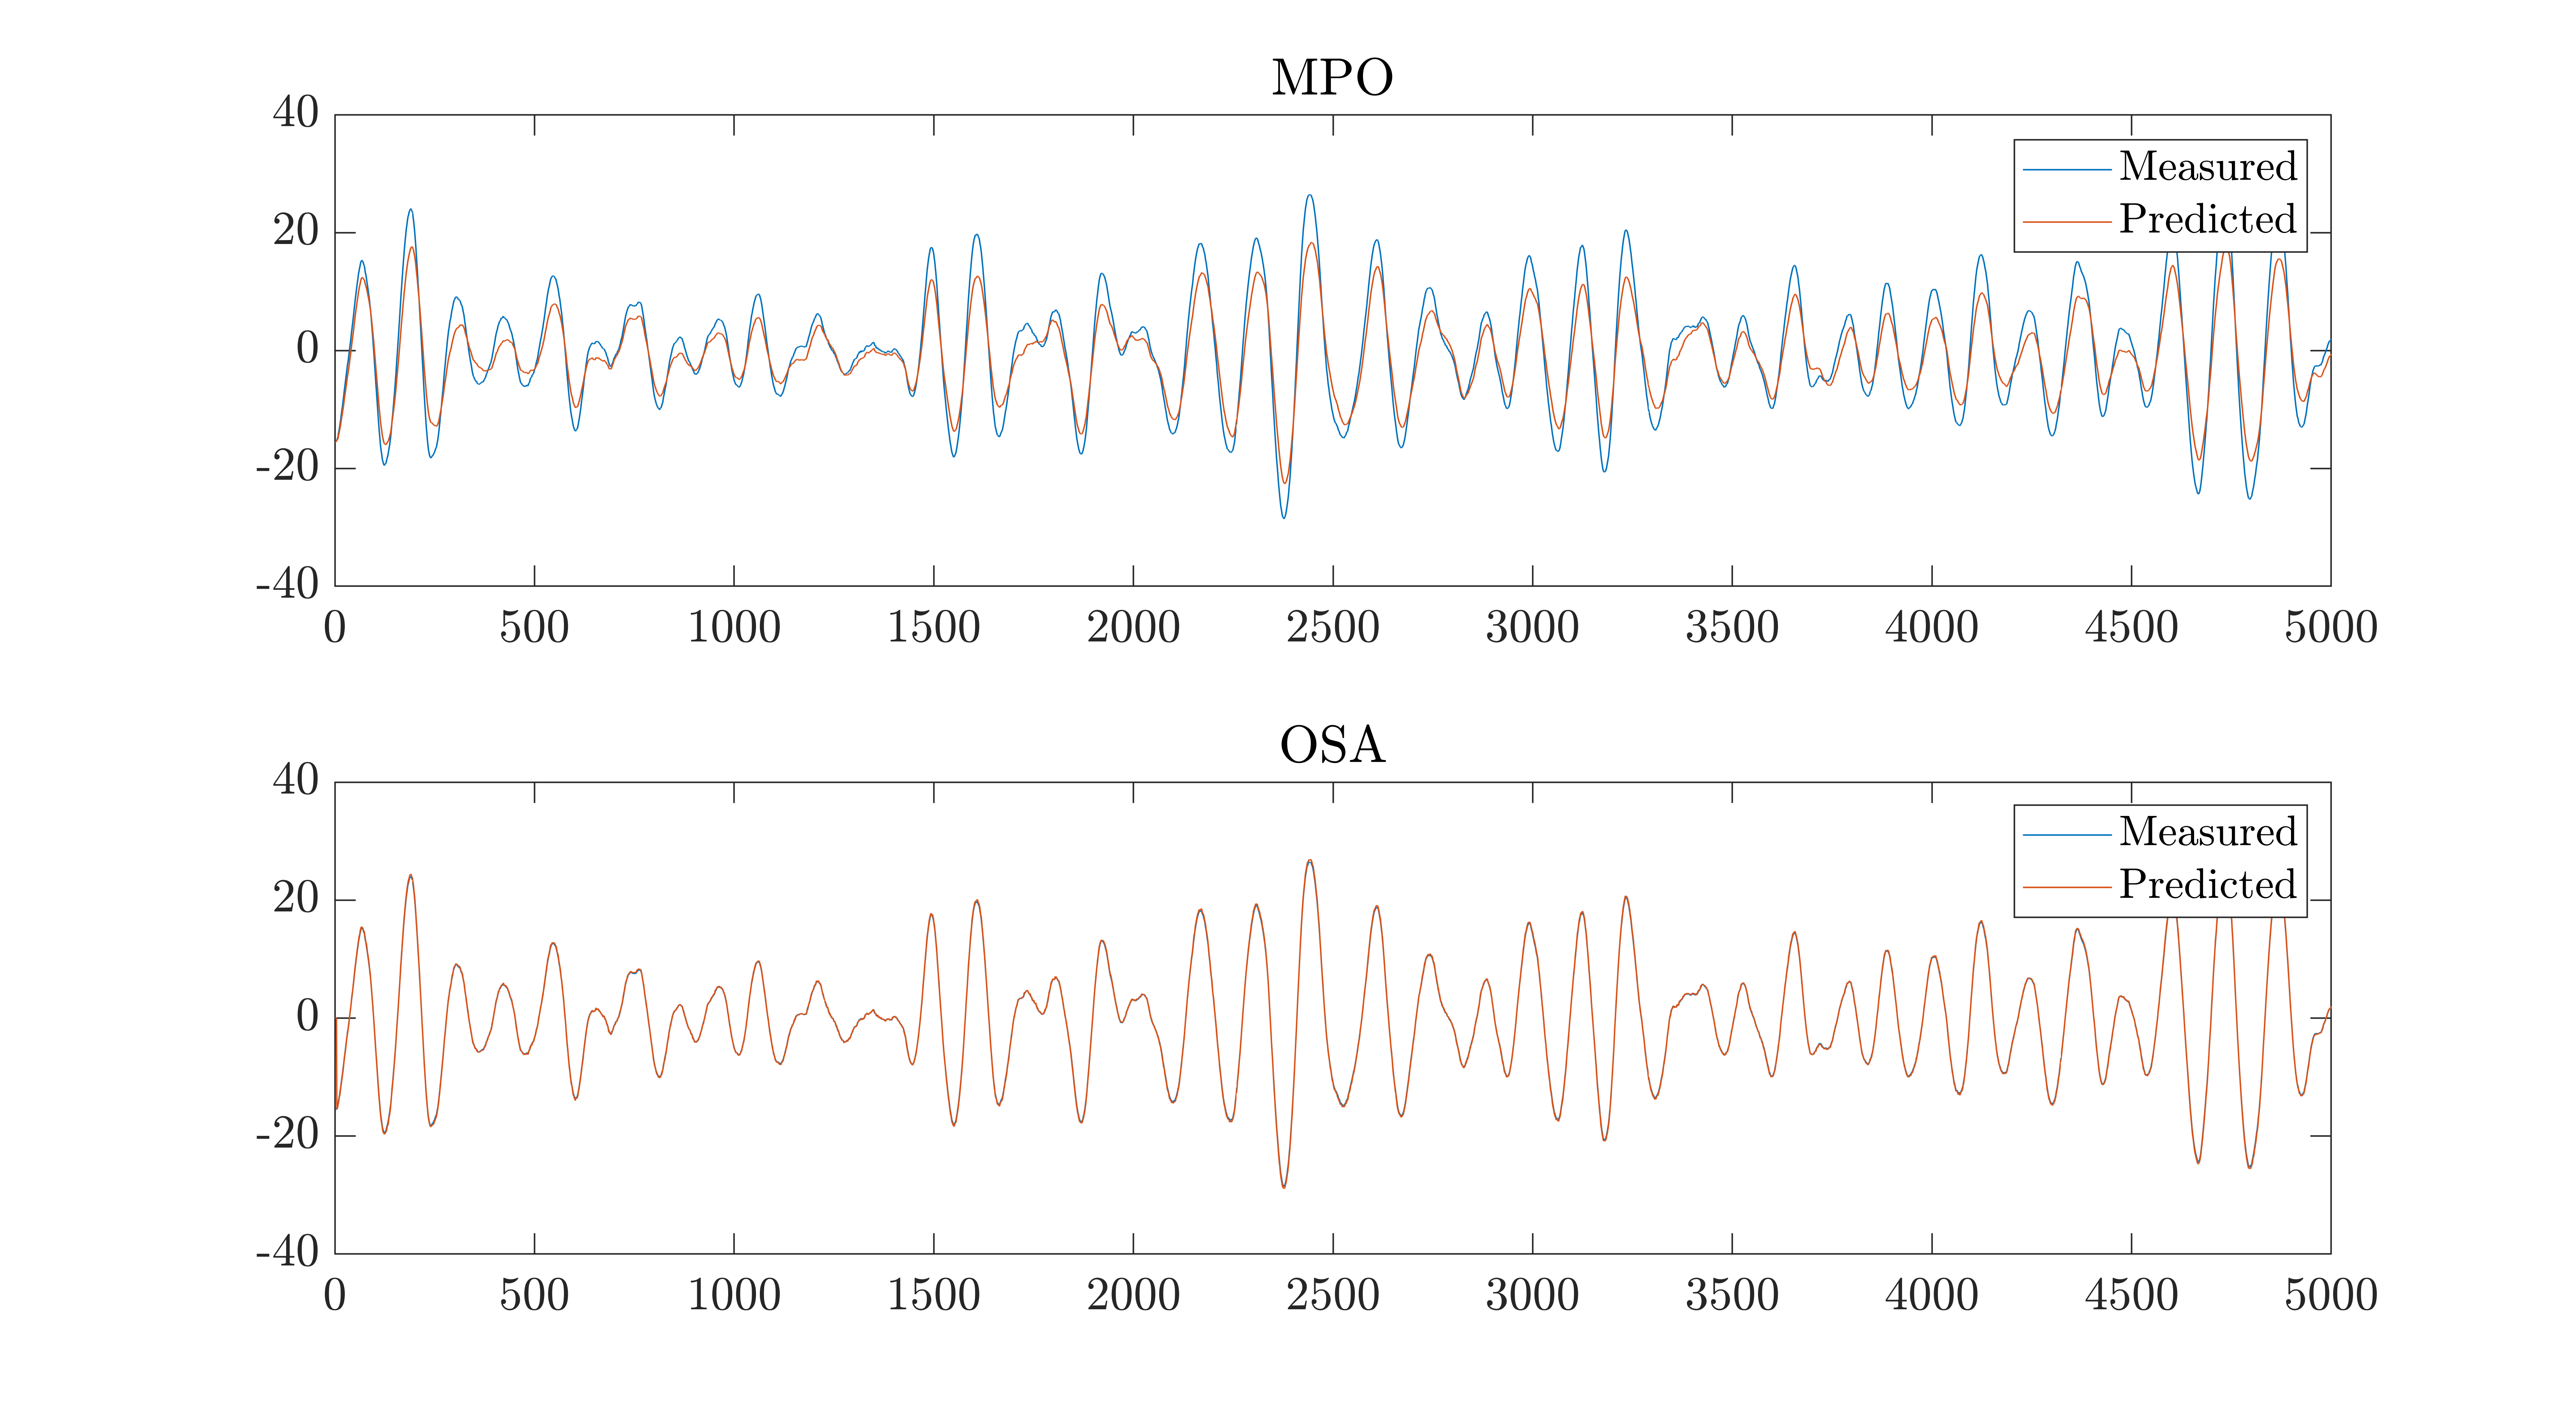
\includegraphics[width=\linewidth]{mpo_osa.png}
	\caption{Model output from the model identified with OSA-PRESS optimal regularisation parameters for dataset HS4.}
\end{figure}
\begin{figure}[!h]
	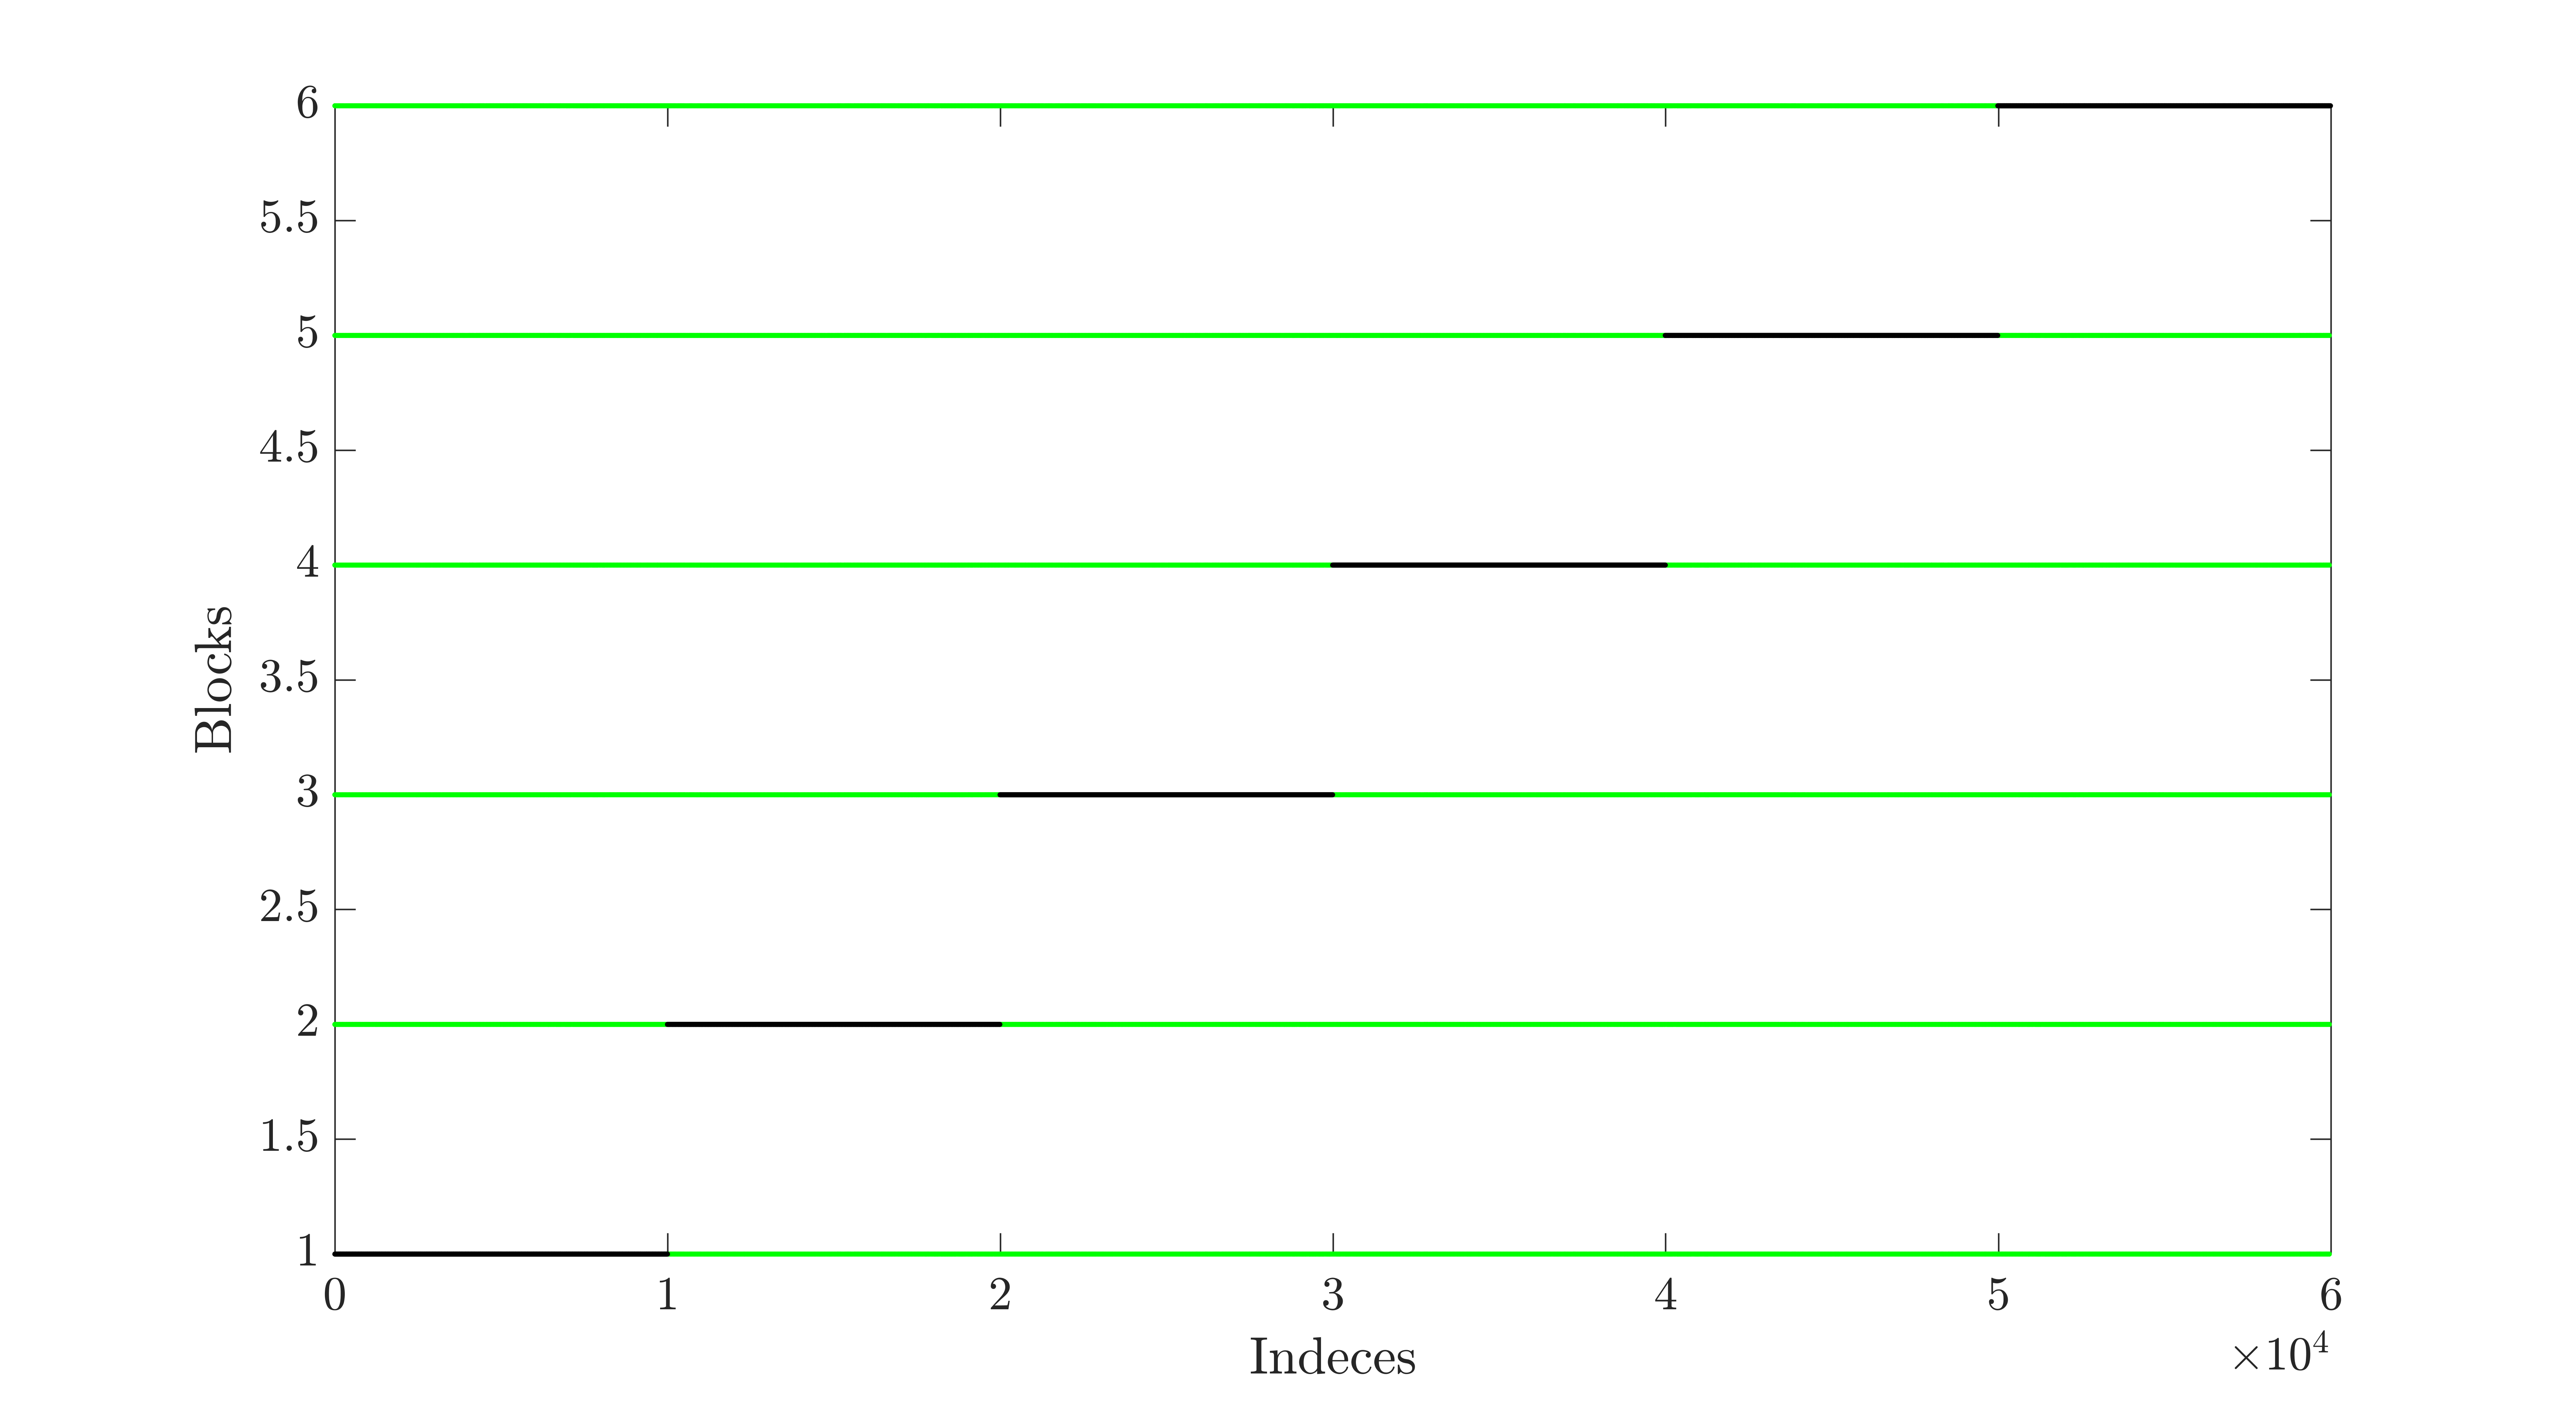
\includegraphics[width=\linewidth]{blocks.png}
	\caption{Block partitions of the regression data. Each testing dataset has time-series structure.}
\end{figure}
\section{Validation results for modified framework}
\par Figures below present validation results for experimental data obtained for soft auxetic foams. The test file indexing corresponds to the tables 2 in the previous report.
%\begin{figure}[!h]
%	\definecolor{mycolor1}{rgb}{0.00000,0.44700,0.74100}%
%	\definecolor{mycolor2}{rgb}{0.85000,0.32500,0.09800}%
%	\centering
%	% This file was created by matlab2tikz.
%
\definecolor{mycolor1}{rgb}{0.00000,0.44700,0.74100}%
\definecolor{mycolor2}{rgb}{0.85000,0.32500,0.09800}%
\definecolor{mycolor3}{rgb}{0.92900,0.69400,0.12500}%
%
\begin{tikzpicture}

\begin{axis}[%
width=6.159cm,
height=2.323cm,
at={(0cm,9.677cm)},
scale only axis,
xmin=0,
xmax=205,
xlabel style={font=\color{white!15!black}},
xlabel={Sample index},
ymin=-32.7588297824386,
ymax=50,
ylabel style={font=\color{white!15!black}},
ylabel={$y(t)$},
axis background/.style={fill=white},
title style={font=\bfseries},
title={VS5: RMSE(OSA) = 0.17972, RMSE(MPO) = 1.6396},
legend style={legend cell align=left, align=left, draw=white!15!black}
]
\addplot [color=mycolor1, line width=2.0pt]
  table[row sep=crcr]{%
6	5.77289099999999\\
7	7.01103000000001\\
8	8.194503\\
9	9.067948\\
10	9.21556799999999\\
11	8.775138\\
12	8.60125300000001\\
13	8.88836699999999\\
14	9.12856300000001\\
15	8.978555\\
16	8.49866499999999\\
17	7.855572\\
18	6.69019499999999\\
19	4.71135899999999\\
20	1.97448399999999\\
21	-1.234825\\
23	-8.976325\\
24	-12.509611\\
25	-15.231824\\
26	-16.997483\\
27	-18.306248\\
28	-18.2675\\
29	-17.493333\\
30	-15.839814\\
31	-13.565403\\
32	-11.100226\\
33	-7.436621\\
34	-2.233689\\
35	2.30662899999999\\
36	5.67105599999999\\
37	8.32544999999999\\
38	10.261391\\
39	11.560061\\
40	11.494084\\
41	10.983531\\
42	9.81798699999999\\
43	7.955647\\
44	6.17193399999999\\
45	4.10680500000001\\
46	2.21438800000001\\
47	0.171670000000006\\
48	-2.85391000000001\\
49	-6.426028\\
50	-10.758991\\
51	-15.378648\\
52	-19.405983\\
53	-22.294667\\
54	-24.107158\\
55	-24.724866\\
56	-23.827501\\
57	-21.527998\\
58	-18.453826\\
59	-14.287585\\
60	-8.702743\\
61	-2.31474600000001\\
63	10.977373\\
64	17.06326\\
65	22.307412\\
66	27.138403\\
67	31.005928\\
68	33.373083\\
69	34.583868\\
70	35.070796\\
71	34.404412\\
72	32.309164\\
73	29.636255\\
74	26.40156\\
75	23.306569\\
76	19.620762\\
77	15.182781\\
79	7.08471399999999\\
83	-9.764274\\
84	-13.763375\\
85	-17.142422\\
86	-20.042206\\
87	-21.913343\\
88	-22.667696\\
89	-22.426453\\
90	-21.744988\\
91	-20.945897\\
92	-18.954787\\
93	-15.942696\\
94	-13.123716\\
95	-9.719954\\
96	-5.59258700000001\\
97	-1.28312399999999\\
98	3.17010500000001\\
99	7.06548699999999\\
100	10.400759\\
101	13.133445\\
102	15.095064\\
103	15.642229\\
104	14.608262\\
106	11.220795\\
107	9.40759199999999\\
108	6.67691600000001\\
109	2.413993\\
110	-3.16741400000001\\
112	-16.744468\\
113	-22.623167\\
114	-27.519926\\
115	-30.848999\\
116	-32.412245\\
117	-32.098029\\
118	-30.384356\\
119	-28.366395\\
120	-25.640747\\
121	-22.084212\\
122	-17.368124\\
123	-12.341884\\
124	-7.92601999999999\\
125	-3.79626500000001\\
126	0.15952200000001\\
127	3.404898\\
128	6.538386\\
129	8.858248\\
130	10.467364\\
131	11.377756\\
132	10.752131\\
133	9.04536999999999\\
136	2.46874299999999\\
137	0.720888000000002\\
138	-0.363222000000007\\
139	-0.607943000000006\\
140	0.00515699999999697\\
141	0.807726000000002\\
142	2.05487099999999\\
143	3.93539100000001\\
144	5.33011500000001\\
145	6.27716100000001\\
146	7.47207\\
148	9.78359499999999\\
149	9.96778499999999\\
150	8.97398899999999\\
151	7.56393399999999\\
152	4.69795500000001\\
154	-1.81043399999999\\
155	-5.59187499999999\\
156	-9.63428999999999\\
157	-13.515889\\
158	-16.929579\\
159	-19.539947\\
160	-20.75069\\
161	-21.079232\\
162	-20.848754\\
163	-19.723718\\
164	-17.351368\\
165	-13.545882\\
166	-9.53237200000001\\
167	-5.25373999999999\\
168	-1.19218100000001\\
169	2.06651600000001\\
170	5.81783899999999\\
171	9.79708400000001\\
172	13.27298\\
173	15.825623\\
174	17.420999\\
175	18.014998\\
176	17.592873\\
177	15.8087\\
178	13.041873\\
180	6.86764099999999\\
181	4.21106900000001\\
182	2.45219599999999\\
183	1.33884699999999\\
184	1.41835399999999\\
185	2.72753900000001\\
186	3.86195799999999\\
187	4.46508900000001\\
188	4.63981200000001\\
189	4.20901599999999\\
190	4.12473399999999\\
191	4.18363099999999\\
192	3.68886900000001\\
193	3.11518799999999\\
194	3.00049300000001\\
195	2.718616\\
196	2.10413299999999\\
197	1.27789799999999\\
198	0.261230000000012\\
199	-1.13391200000001\\
200	-3.082964\\
201	-5.698317\\
204	-12.501065\\
205	-13.981202\\
};
\addlegendentry{True output}

\addplot [color=mycolor2, dashed, line width=2.0pt]
  table[row sep=crcr]{%
6	5.86334857868346\\
7	7.261572034528\\
8	8.13076354732175\\
9	9.2375588503117\\
11	8.95774612160409\\
12	8.73264780719887\\
13	8.83957621564286\\
14	9.195571142587\\
15	8.72450871691714\\
16	8.79627677644723\\
17	7.88531550945044\\
18	6.88117218653309\\
19	4.77854668048997\\
20	2.15959579276529\\
21	-1.06303417564465\\
22	-5.05222363394719\\
24	-12.6735773416913\\
25	-15.2823409420941\\
26	-17.100608301693\\
27	-18.2922154724351\\
28	-18.4756570498334\\
29	-17.4294757477608\\
30	-16.0338383730949\\
31	-13.3820571863169\\
32	-11.0713229417489\\
33	-7.67227720833839\\
34	-2.31077431534382\\
35	2.57204602969009\\
36	5.77034922738378\\
37	8.55592975265384\\
38	10.2476604849288\\
39	11.5687358519285\\
40	11.6768119587787\\
41	11.11912684256\\
42	9.88662142992786\\
43	7.65209494764139\\
44	5.98424655445544\\
45	4.19392903626257\\
47	0.242270085696646\\
48	-2.88255579634114\\
49	-6.41927007805654\\
50	-10.42254317365\\
51	-15.1875549979082\\
52	-19.6005122306592\\
53	-22.5130008354558\\
54	-24.2169413466248\\
55	-24.9254435876311\\
56	-23.8675751054423\\
57	-21.7136358472196\\
58	-18.7685149325907\\
59	-14.3858421304434\\
60	-8.84421307986906\\
63	10.8681832579242\\
64	17.2087859327762\\
66	27.1796546613149\\
67	31.2119788481677\\
68	33.2806448598164\\
69	34.6192597816969\\
70	35.0270938493873\\
71	34.4376496244478\\
72	32.3363518925019\\
74	26.3523644826482\\
76	19.7791016092105\\
77	15.1241658328247\\
80	2.92317628130141\\
81	-1.33195983747103\\
82	-5.36590090703166\\
83	-9.76095929876084\\
84	-13.7877471394254\\
85	-16.9719918704361\\
86	-19.7916354923879\\
87	-21.984654486439\\
88	-22.7347563446429\\
89	-22.4015129488174\\
90	-21.543470446786\\
91	-20.8083577223888\\
92	-18.9333406872196\\
93	-15.9127451298621\\
94	-13.1168510128132\\
95	-9.6598781758361\\
96	-5.45761293211723\\
97	-1.4119735910129\\
98	3.05130347316589\\
99	7.10057643691275\\
100	10.5591294672406\\
101	13.193953012461\\
102	14.9704782797689\\
103	15.9260358208745\\
104	14.5606577793916\\
105	13.0375720943161\\
106	11.0890292577258\\
107	9.22076164111536\\
108	7.00319687992146\\
109	2.70875059306411\\
110	-2.88905458965863\\
112	-16.7364405124733\\
113	-22.6116198604843\\
114	-27.3227160999006\\
115	-31.1111280766867\\
116	-32.7588297824387\\
117	-32.3695639149215\\
118	-30.3045399666283\\
119	-28.0722658989315\\
120	-25.6662153048512\\
121	-22.3089250327032\\
122	-17.5107812571887\\
123	-12.1604238985922\\
124	-7.64813010497915\\
125	-3.76679916552186\\
126	-0.0547011042512793\\
128	6.53983979734974\\
129	9.2835348943054\\
130	10.1943540801032\\
131	11.3334004345404\\
132	10.6972599486067\\
133	9.10225948698613\\
134	7.10601129487273\\
135	4.35077611292454\\
136	2.15682951914056\\
137	0.404746011841041\\
138	-0.501104320773152\\
139	-0.635027577025483\\
140	-0.319523140473251\\
141	0.60030102416809\\
142	1.89102677765825\\
143	4.10565389906904\\
144	5.55099440041894\\
145	6.21479749321688\\
146	7.34397705282083\\
147	8.60537846889491\\
148	9.94435863056481\\
149	10.23951927551\\
150	9.05478184418465\\
151	7.47711037775488\\
152	4.93135112340087\\
153	1.31963299534482\\
154	-1.46352048696929\\
156	-9.83655153270888\\
157	-13.6704208477479\\
158	-16.7365572887481\\
159	-19.6626387863235\\
160	-20.9302261368496\\
161	-21.1088593925475\\
162	-21.1243123581067\\
163	-19.663604485112\\
164	-17.4277411765712\\
165	-13.6644106559011\\
166	-9.61547199038827\\
168	-0.926248982144728\\
169	1.99275865337785\\
170	5.69538434437598\\
171	9.77190005210315\\
172	13.4528112550579\\
173	16.0001039033063\\
174	17.5335266673401\\
175	18.0651745401799\\
176	17.6304536994657\\
177	16.1079220930243\\
178	13.2552136152013\\
179	9.8136219366892\\
180	6.82369470379007\\
181	3.72656471550624\\
182	2.54710940763081\\
183	1.2479152420706\\
184	1.02169381469744\\
186	4.01062967460453\\
187	4.55497457833317\\
188	5.03881217259101\\
189	4.16701307749872\\
190	3.96264336856208\\
191	4.34865392895227\\
192	3.99370220553311\\
193	3.10259588589466\\
194	2.82152132943304\\
195	2.6825446164934\\
196	2.03728005998485\\
197	1.86264953207152\\
198	0.176752593463902\\
199	-1.02146453443692\\
200	-3.14320759267471\\
201	-5.4960982921742\\
202	-7.65106539064206\\
203	-10.3357490688439\\
204	-12.7036668040134\\
205	-14.119950684985\\
};
\addlegendentry{OSA predition}

\addplot [color=mycolor3, line width=3.0pt, draw=none, mark=*, mark options={solid, mycolor3}]
  table[row sep=crcr]{%
6	5.77289099999999\\
7	7.01103000000001\\
8	8.194503\\
9	9.067948\\
10	9.08878318788462\\
11	8.7837717569401\\
12	8.79746468379858\\
13	9.04385394019815\\
14	9.39772603307085\\
15	9.12104867477842\\
16	8.85331393716649\\
17	8.36371307592981\\
18	7.36185370303929\\
19	5.59009497180782\\
20	3.15254199726746\\
21	0.254857007446191\\
22	-3.41181415839421\\
23	-7.03056017029147\\
24	-10.6088266284843\\
25	-13.4115214948502\\
26	-15.3607325240525\\
27	-16.8992787792229\\
28	-17.3447592965989\\
29	-16.8918367954115\\
30	-15.78333991146\\
31	-13.8202000390042\\
32	-11.6475165249364\\
33	-8.59667650893513\\
34	-3.78943450310175\\
35	0.79413047539731\\
36	4.05306542687873\\
37	6.81781630363923\\
38	8.92045926522175\\
39	10.3508069899742\\
40	10.6784102556262\\
41	10.6336538358613\\
42	9.85557502542756\\
43	8.08420939133592\\
44	6.40235901603151\\
45	4.65932618183453\\
46	2.91200831275373\\
47	1.0211899822792\\
48	-1.85418285066888\\
49	-5.34591800962974\\
50	-9.30151384028795\\
51	-13.6044090647039\\
52	-17.7594749332418\\
53	-20.8199202687059\\
54	-22.7904614383704\\
55	-23.8757453557152\\
56	-23.3743172201324\\
57	-21.591077734315\\
58	-19.3023364362398\\
59	-15.7030928068862\\
60	-10.6934939180341\\
61	-4.74957334740967\\
62	1.42330606772043\\
63	7.63270053185846\\
64	13.7229502014212\\
65	18.8954903109222\\
66	23.7863258669614\\
67	28.1354602871317\\
68	30.8002951934832\\
69	32.3778329344369\\
70	33.3969425968551\\
71	33.2885238069493\\
72	31.7521783661999\\
73	29.4193589469944\\
74	26.6017007017619\\
75	23.7353636986978\\
76	20.4674851865186\\
77	16.3415438570069\\
78	12.4161566349389\\
79	8.5431162438289\\
80	4.5347366075186\\
81	0.384375326942859\\
82	-3.4522547389482\\
83	-7.3989807737677\\
84	-11.4327306324937\\
85	-14.6394264099177\\
86	-17.3740466619699\\
87	-19.4798357481406\\
88	-20.4905684618432\\
89	-20.4582633738112\\
90	-19.9819343328872\\
91	-19.4342934481843\\
92	-17.7820870761267\\
93	-15.1034775448227\\
94	-12.6397670849979\\
95	-9.56000921778514\\
96	-5.64037755264781\\
97	-1.74674962848911\\
98	2.28091367223618\\
99	5.98009296744326\\
100	9.24313563230078\\
101	11.8668569025795\\
102	13.6464324763297\\
103	14.462107068411\\
104	13.5301397162604\\
105	11.9948718107797\\
106	10.4439326995995\\
107	8.63019781983778\\
108	6.36771038682662\\
109	2.71655365097865\\
110	-2.30556924870473\\
111	-8.46500000223102\\
112	-14.7818866984962\\
113	-20.2355569621568\\
114	-24.5980044725723\\
115	-27.9128835132115\\
116	-29.7725063867359\\
117	-29.7958420980652\\
118	-28.3726111199934\\
119	-26.5490441367353\\
120	-24.2993505314242\\
121	-21.4237712752625\\
122	-17.3047509235259\\
123	-12.6392294092668\\
124	-8.46528442778782\\
125	-4.6931006231583\\
126	-1.22100276866036\\
127	1.67222464688973\\
128	4.59054679086537\\
129	7.13026360304102\\
130	8.500578839718\\
131	9.30499447700871\\
132	8.8371985509589\\
133	7.2719903244319\\
134	5.48284728779885\\
135	3.32515565798371\\
136	0.995255081923119\\
137	-0.796885610617153\\
138	-1.91079550257984\\
139	-2.12506466655771\\
140	-1.7243139061118\\
141	-1.09224271672562\\
142	0.0770203041815023\\
143	2.13670915375673\\
144	3.87730179749508\\
145	4.99078678165756\\
146	6.34008789945187\\
147	7.81621563548208\\
148	9.45949671310061\\
149	10.2385771155382\\
150	9.76439318934058\\
151	8.70605496643358\\
152	6.47953381935463\\
153	3.54333557887966\\
154	0.905575063875318\\
155	-2.47263906504824\\
156	-6.54953140794836\\
157	-10.5179181128261\\
158	-13.8182841774751\\
159	-16.7996661952624\\
160	-18.602344769625\\
161	-19.3621869611084\\
162	-19.9881858343878\\
163	-19.5543586582368\\
164	-17.8608927404508\\
165	-14.903507350879\\
166	-11.5969112676515\\
167	-7.83323675067302\\
168	-3.98546855574074\\
169	-1.06469573066556\\
170	2.40531356531025\\
171	6.39092544442897\\
172	10.1301031702551\\
173	13.0667388882672\\
174	15.1577997845632\\
175	16.3343554486084\\
176	16.5468074649802\\
177	15.699806252524\\
178	13.9130223084386\\
179	11.4384186701498\\
180	8.97384861567761\\
181	6.50708951431213\\
182	5.08666345191295\\
183	4.16963428156487\\
184	3.82966041120957\\
185	4.71501342705884\\
186	5.73727411609329\\
187	5.99616236185912\\
188	6.07414065000066\\
189	5.37482414544806\\
190	4.73536938701722\\
191	4.60229479361311\\
192	4.12762044164765\\
193	3.21614006261828\\
194	2.66789897468934\\
195	2.17914078490745\\
196	1.2495726529659\\
197	0.70198073079365\\
198	-0.361082517169507\\
199	-1.76092820884855\\
200	-3.58052289665238\\
201	-5.92438255320116\\
202	-7.73593080830025\\
203	-9.81777855176699\\
204	-11.942174734039\\
205	-13.3125513092952\\
};
\addlegendentry{MPO prediction}

\end{axis}

\begin{axis}[%
width=6.159cm,
height=2.323cm,
at={(8.104cm,9.677cm)},
scale only axis,
xmin=0,
xmax=205,
xlabel style={font=\color{white!15!black}},
xlabel={Sample index},
ymin=-50,
ymax=31.143746,
ylabel style={font=\color{white!15!black}},
ylabel={$y(t)$},
axis background/.style={fill=white},
title style={font=\bfseries},
title={VS10: RMSE(OSA) = 0.21681, RMSE(MPO) = 3.3093},
legend style={legend cell align=left, align=left, draw=white!15!black}
]
\addplot [color=mycolor1, line width=2.0pt]
  table[row sep=crcr]{%
6	18.682806\\
7	15.74997\\
9	10.576403\\
10	7.56778800000001\\
11	5.42792800000001\\
13	1.68376900000001\\
14	0.17983799999999\\
15	-1.10781499999999\\
16	-1.381146\\
17	-1.731178\\
18	-1.627207\\
19	-1.919724\\
20	-2.68358599999999\\
21	-3.87275600000001\\
22	-5.363575\\
23	-6.156341\\
24	-5.936126\\
25	-5.15923599999999\\
27	-3.474593\\
28	-2.53923399999999\\
29	-1.54485199999999\\
30	-0.397446000000002\\
31	0.391507999999988\\
32	0.47369599999999\\
33	-0.255188000000004\\
34	-1.22033099999999\\
35	-2.007609\\
36	-2.06726\\
37	-2.06583599999999\\
38	-1.95595900000001\\
40	-0.63575800000001\\
41	0.539378999999997\\
42	2.851449\\
43	5.946901\\
44	9.95119700000001\\
45	15.036711\\
46	19.697882\\
47	23.30326\\
48	25.764625\\
49	27.531037\\
50	29.00799\\
51	30.318054\\
52	30.681449\\
53	29.751536\\
54	27.189132\\
56	20.567264\\
57	16.682732\\
59	6.682571\\
60	0.933018000000004\\
61	-6.10607300000001\\
62	-13.381507\\
63	-20.310762\\
64	-25.737931\\
65	-30.11203\\
66	-33.762146\\
67	-36.925335\\
68	-39.973829\\
69	-41.32662\\
70	-40.821554\\
71	-39.299779\\
72	-36.39459\\
73	-31.8252\\
74	-25.603716\\
76	-11.301423\\
77	-3.81570199999999\\
78	3.906362\\
79	10.755105\\
80	16.503108\\
81	20.842439\\
82	24.194173\\
83	26.519941\\
84	27.800389\\
85	27.231064\\
86	25.249212\\
87	21.756476\\
89	13.682663\\
90	7.87789900000001\\
91	0.459620999999999\\
92	-8.47745900000001\\
93	-17.823048\\
94	-25.448388\\
95	-31.230155\\
96	-36.076939\\
97	-39.615838\\
98	-41.537703\\
99	-41.282426\\
100	-39.180476\\
101	-35.30805\\
102	-29.914017\\
103	-23.320299\\
104	-15.747489\\
106	0.424893999999995\\
107	7.554802\\
108	13.949292\\
109	19.530532\\
110	23.69028\\
111	26.900092\\
112	29.601528\\
113	30.837615\\
114	30.608561\\
115	29.300591\\
116	26.681175\\
119	16.634517\\
120	13.099891\\
121	9.196969\\
123	0.910775000000001\\
124	-2.12016700000001\\
126	-6.49552299999999\\
127	-8.39292499999999\\
128	-9.43104\\
129	-9.34449499999999\\
130	-7.876046\\
131	-5.999337\\
132	-4.401825\\
133	-3.37652800000001\\
134	-1.75471999999999\\
135	0.0323439999999948\\
136	2.213382\\
137	4.31340599999999\\
138	5.29232999999999\\
139	5.86152999999999\\
140	5.85838799999999\\
141	5.36789899999999\\
142	4.72949800000001\\
143	3.54644400000001\\
145	0.114281000000005\\
146	-1.30323100000001\\
147	-2.90153900000001\\
148	-4.29282800000001\\
149	-6.08894000000001\\
150	-8.600112\\
151	-11.450006\\
154	-18.794726\\
155	-20.139642\\
156	-20.793836\\
157	-19.915992\\
158	-18.004557\\
159	-15.308608\\
160	-11.485403\\
161	-6.875674\\
162	-1.921358\\
163	3.322836\\
164	9.11876100000001\\
165	14.643156\\
167	24.969052\\
168	28.34722\\
169	30.457757\\
170	31.143746\\
171	29.929484\\
172	27.600072\\
173	24.294542\\
174	19.907792\\
175	14.719772\\
176	9.01960800000001\\
178	-1.31093899999999\\
180	-10.734527\\
181	-15.832986\\
182	-19.914652\\
183	-22.604401\\
184	-24.338558\\
185	-24.932347\\
186	-23.486434\\
188	-15.479519\\
189	-10.980546\\
191	-0.135928000000007\\
193	10.735584\\
194	15.895538\\
195	19.959233\\
196	23.231251\\
197	25.517014\\
198	26.341323\\
199	25.925733\\
200	24.816531\\
201	22.908364\\
202	19.699138\\
204	12.042172\\
205	7.8092\\
};
\addlegendentry{True output}

\addplot [color=mycolor2, dashed, line width=2.0pt]
  table[row sep=crcr]{%
6	18.8879535010905\\
8	12.5768483838652\\
9	10.644610059596\\
10	7.63434850430588\\
11	5.30994701082375\\
12	3.78650408619691\\
13	1.17881391906249\\
14	0.429512367789329\\
15	-0.994644017452231\\
16	-1.33755151027455\\
17	-1.76750778456133\\
18	-1.58368174081036\\
19	-1.83224532948572\\
20	-2.60717332459569\\
21	-3.55747107054034\\
22	-5.59718441522907\\
23	-6.30999598889832\\
24	-6.22904977954209\\
25	-4.86725028584641\\
26	-4.25509196112705\\
27	-3.76296250420461\\
28	-2.39961081250561\\
29	-1.52519464835652\\
30	-0.344242109047912\\
31	0.677844037522505\\
32	0.187750435237234\\
33	0.00576711323000723\\
34	-1.39756131897522\\
35	-1.82047571052277\\
36	-2.17514639753264\\
37	-2.15656854915622\\
38	-2.19530493028549\\
39	-1.1515358382544\\
40	-0.752453631556335\\
41	0.477110473601897\\
42	2.67958089753188\\
43	5.78068681096835\\
44	9.7664500048802\\
45	15.1805336649494\\
46	19.6871598252226\\
47	23.2786324865701\\
48	25.97638944817\\
49	27.448744192311\\
50	28.7915331668268\\
51	30.2425852232503\\
52	30.7384511534575\\
53	29.5224091125028\\
54	27.242534386686\\
55	23.9550137439485\\
56	20.2461790362192\\
57	16.7357498472005\\
58	11.7801688401961\\
59	6.49711821435429\\
60	1.40266026378958\\
61	-6.12062272954563\\
63	-20.3075786478856\\
64	-25.8296473642423\\
65	-30.0041226654301\\
66	-33.3497145984124\\
67	-36.9254324180865\\
68	-39.6626115449937\\
69	-41.4814382825916\\
70	-40.601426114219\\
71	-39.0402563285241\\
72	-36.5699926158285\\
73	-31.9637020684091\\
74	-25.4754883286873\\
75	-18.6015970300656\\
76	-10.8337933835214\\
77	-4.13648058875216\\
78	3.73283015252031\\
79	11.0670787757036\\
80	16.4005610660169\\
81	21.170576857\\
82	23.7745064768364\\
83	26.2654960879779\\
84	27.8197433865911\\
85	27.5016731348728\\
86	24.9520729713619\\
87	21.5729606597046\\
88	17.4450070534067\\
89	13.9310756818447\\
90	7.97288307002634\\
91	0.856881351411147\\
93	-18.0378989376727\\
94	-25.3288834714775\\
95	-30.9852715747755\\
96	-36.1293357055321\\
97	-39.83111260228\\
98	-41.4650013856445\\
99	-41.0864667956909\\
100	-38.9835650206778\\
101	-35.1182779960938\\
102	-30.2712566939862\\
103	-23.4482637612259\\
105	-7.29650202281528\\
106	0.295656514624511\\
107	7.35701879915001\\
108	14.0821152106033\\
109	19.4106354896881\\
110	23.9951810553293\\
112	29.3115414506061\\
113	30.5640483545329\\
114	30.9840847387188\\
115	29.1712240904281\\
116	26.4440793207757\\
118	19.7563388631404\\
119	16.7235396878928\\
120	13.3077668160408\\
121	8.81280634450852\\
123	1.09819330721456\\
124	-2.22655728293506\\
125	-4.22666957822267\\
126	-6.40219583629298\\
127	-8.7553418106065\\
128	-9.33846908557541\\
129	-9.11147920074171\\
130	-8.15465242689044\\
131	-5.85968913864485\\
132	-4.35691488645003\\
133	-3.32106210663252\\
134	-1.83264842403926\\
135	0.157622784468003\\
136	2.07388115211819\\
137	4.20910773993413\\
138	5.29920756490012\\
139	6.26054128269843\\
140	5.53637838197147\\
141	5.39084217101367\\
142	4.86491885279281\\
143	3.26115653675203\\
144	2.02270589687009\\
146	-1.60914552549107\\
147	-2.91057340032725\\
148	-3.89822478876698\\
149	-6.22042719771176\\
150	-8.37278485115303\\
152	-14.2462261241022\\
153	-15.9620895301953\\
154	-18.9156006039207\\
155	-20.2484478925156\\
156	-20.9301472641349\\
157	-19.8655422580627\\
158	-17.9723648114871\\
159	-15.4707018109229\\
160	-11.2586937541687\\
161	-7.20594669982046\\
162	-2.02127564862329\\
163	3.7066981749206\\
164	8.78897672877233\\
165	14.5044998863473\\
166	19.7271170014895\\
167	25.1480748591054\\
168	28.459977714072\\
169	30.3470037955491\\
170	30.9949519876785\\
171	29.9198411871605\\
172	27.5888572639963\\
173	24.0735784079299\\
174	19.8977166130501\\
175	14.6291789536355\\
176	8.88121008750775\\
177	3.65837027570132\\
178	-1.03290543176135\\
179	-6.14466012109969\\
180	-10.6649754550444\\
181	-15.8682407280504\\
182	-19.6146676335727\\
183	-22.4966615842552\\
184	-24.6374944162402\\
185	-24.6500369360483\\
186	-23.8068089480315\\
189	-10.8279172384248\\
190	-5.68245756258773\\
191	-0.34467265008729\\
192	5.51210172558316\\
193	10.9703100726755\\
194	15.7688897730433\\
195	19.6768301833393\\
196	23.4359778703069\\
197	25.4425521520809\\
198	26.2951507943809\\
199	26.0233110503841\\
200	24.3277442944814\\
201	22.8484217206592\\
202	19.9890351874036\\
203	15.5559155547558\\
204	12.0958684189046\\
205	7.62498131986985\\
};
\addlegendentry{OSA predition}

\addplot [color=mycolor3, line width=3.0pt, draw=none, mark=*, mark options={solid, mycolor3}]
  table[row sep=crcr]{%
6	18.682806\\
7	15.74997\\
8	13.12402\\
9	10.576403\\
10	7.63434850430588\\
11	5.42909018299434\\
12	3.7451003278666\\
13	1.55102880138693\\
14	0.0543591717487857\\
15	-1.18248516841032\\
16	-1.3496964885953\\
17	-1.64018911585487\\
18	-1.4301024868295\\
19	-1.54999967232976\\
20	-2.09458379085271\\
21	-2.78707706065174\\
22	-4.11714563493086\\
23	-4.90758067264659\\
24	-5.0319318225651\\
25	-4.30044460296895\\
26	-3.54072497848526\\
27	-3.08711077077282\\
28	-2.36559576389271\\
29	-1.60580877845365\\
30	-0.61928598455151\\
31	0.299166540132603\\
32	0.187685354672141\\
33	-0.396487073765343\\
34	-1.45361572623867\\
35	-2.08331469913327\\
36	-2.13973386700886\\
37	-2.18932128900968\\
38	-2.36150851271432\\
39	-1.78076736724103\\
40	-1.33616366770292\\
41	-0.367941773628871\\
42	1.6098619596479\\
43	4.29385822400204\\
44	7.80089639885048\\
45	12.6637543201309\\
46	17.1685316672417\\
47	20.7144014843641\\
48	23.4348817681302\\
49	25.4362808108431\\
50	27.0351330943832\\
51	28.4911976832799\\
52	29.1266164403941\\
53	28.2841229567666\\
54	25.9524321608748\\
55	22.9732098661756\\
56	19.6371656332016\\
57	15.8999107491863\\
58	11.1471395076013\\
59	6.14229396547677\\
60	0.952553638684037\\
61	-5.63331350979831\\
62	-12.3002763330875\\
63	-18.7084403781615\\
64	-23.7772800493852\\
65	-27.7721953652636\\
66	-30.7720073774856\\
67	-33.4959471115633\\
68	-35.9357657249183\\
69	-37.1034780897142\\
70	-36.3528642227763\\
71	-34.6020135985513\\
72	-31.8938730963803\\
73	-27.8262514148564\\
74	-22.1457082131278\\
75	-15.8477681351322\\
76	-9.04470071622274\\
77	-2.43889070152414\\
78	4.2875979160589\\
79	10.4713678485622\\
80	15.4434837931277\\
81	19.4419066991468\\
82	22.0454663219757\\
83	23.5586899370582\\
84	24.1926101700558\\
85	23.3971755371994\\
86	21.0145755395148\\
87	17.1702412892305\\
88	12.707892798871\\
89	8.64281647120035\\
90	3.11377263473867\\
91	-3.42937555680109\\
92	-11.6149217318746\\
93	-20.2359328724091\\
94	-26.8972431589878\\
95	-31.4420880151509\\
96	-35.1458376837909\\
97	-37.8015468758526\\
98	-38.8487164573195\\
99	-37.7054355339743\\
100	-34.7433403183237\\
101	-30.0856437085222\\
102	-24.5566727638287\\
103	-18.1445843006165\\
104	-10.6563520836093\\
105	-2.57028585314958\\
106	4.95703269120003\\
107	11.2932846411763\\
108	16.9188948457599\\
109	21.4915169402098\\
110	24.9310898491533\\
111	27.0601060883488\\
112	28.4764236711825\\
113	28.2510899787628\\
114	27.102946653538\\
115	24.8437555228039\\
116	21.2759018217843\\
117	16.9703779535\\
118	12.7151094919119\\
119	8.84605604327461\\
120	5.3574667889705\\
121	1.42042986728984\\
122	-2.50504491270161\\
123	-5.84030030657055\\
124	-7.94813437064542\\
125	-8.85734333665224\\
126	-9.47777440825766\\
127	-10.1060651559837\\
128	-9.67786765703639\\
129	-7.95941829738922\\
130	-5.26958437249263\\
131	-2.13196951516386\\
132	0.521517330786025\\
133	2.42295389566661\\
134	4.55031417317852\\
135	6.69312834778074\\
136	8.76429572300259\\
137	10.4035751645026\\
138	10.6948178756864\\
139	10.757689269722\\
140	9.68206294341456\\
141	8.07827457077215\\
142	6.34291718758263\\
143	3.7252239759826\\
144	0.840455828599858\\
145	-1.92250264834138\\
146	-4.56864892763218\\
147	-7.18421779418722\\
148	-9.00094715536048\\
149	-11.194628719752\\
150	-13.5973206802846\\
151	-16.0265036787984\\
152	-18.2087405157547\\
153	-19.7217255608313\\
154	-21.1320006916339\\
155	-21.5138189181102\\
156	-21.3073472242808\\
157	-19.4986157791365\\
158	-16.689431881397\\
159	-13.3457365881346\\
160	-8.73617401688921\\
161	-3.86627215667411\\
162	1.17247182900158\\
163	6.73116316807929\\
164	12.298246270944\\
165	17.3998325702669\\
166	21.9530165324926\\
167	26.5492751732351\\
168	29.4404086180631\\
169	30.9226609828889\\
170	30.8501297135655\\
171	28.9111381956854\\
172	25.8971455883566\\
173	21.7704223065364\\
174	16.6995317652014\\
175	10.8689274631217\\
176	4.5753474848357\\
177	-1.16056955535825\\
178	-6.32260459536295\\
179	-11.0038968215676\\
180	-15.2690794584105\\
181	-19.8333845511372\\
182	-22.889207230976\\
183	-24.3795028630093\\
184	-25.1535588117331\\
185	-24.4422069148989\\
186	-22.1386207643292\\
187	-17.3031598449842\\
188	-12.2875260027175\\
189	-6.86973872798987\\
190	-0.878254889485788\\
191	4.76801282922284\\
192	10.4051362100707\\
193	15.8853856030006\\
194	20.7913178618211\\
195	24.1607060797336\\
196	26.8207572855887\\
197	28.2538058208495\\
198	28.1211302667047\\
199	26.7979631474946\\
200	24.2652760645691\\
201	20.9996764547408\\
202	16.8056027108888\\
203	11.7779317311579\\
204	6.98178692382467\\
205	1.83800436085752\\
};
\addlegendentry{MPO prediction}

\end{axis}

\begin{axis}[%
width=6.159cm,
height=2.323cm,
at={(0cm,6.452cm)},
scale only axis,
xmin=0,
xmax=205,
xlabel style={font=\color{white!15!black}},
xlabel={Sample index},
ymin=-30.183552,
ymax=50,
ylabel style={font=\color{white!15!black}},
ylabel={$y(t)$},
axis background/.style={fill=white},
title style={font=\bfseries},
title={VS15: RMSE(OSA) = 0.14857, RMSE(MPO) = 5.5885},
legend style={legend cell align=left, align=left, draw=white!15!black}
]
\addplot [color=mycolor1, line width=2.0pt]
  table[row sep=crcr]{%
6	8.63662099999999\\
7	5.02228700000001\\
8	1.209575\\
9	-3.08779000000001\\
10	-6.685315\\
11	-10.722016\\
12	-14.355169\\
13	-16.963607\\
14	-18.384954\\
15	-19.592331\\
16	-20.437192\\
17	-20.522362\\
18	-19.727378\\
19	-18.145541\\
20	-15.626255\\
21	-12.037238\\
23	-3.55190400000001\\
24	-0.13838100000001\\
25	2.95940300000001\\
26	6.387764\\
27	9.58119600000001\\
28	12.227314\\
30	17.16609\\
32	21.736441\\
35	27.25057\\
36	28.639896\\
37	28.713329\\
38	28.354503\\
39	27.673441\\
40	26.231514\\
41	23.874686\\
42	20.823343\\
43	18.232425\\
45	12.703332\\
46	8.58389299999999\\
47	3.87346500000001\\
48	-1.22831400000001\\
49	-6.005888\\
50	-11.006781\\
52	-22.228474\\
53	-26.248954\\
54	-28.792048\\
55	-30.183552\\
56	-29.535729\\
57	-27.463791\\
58	-24.206147\\
59	-20.486483\\
60	-16.974504\\
62	-9.27648400000001\\
64	-0.604590999999999\\
65	4.008973\\
66	8.81898899999999\\
67	12.774712\\
68	15.570924\\
69	17.189394\\
71	18.413746\\
72	17.906921\\
73	16.380704\\
74	14.101837\\
75	10.884639\\
76	7.78006500000001\\
77	4.06052700000001\\
79	-3.729829\\
81	-10.788199\\
83	-18.647504\\
84	-22.058303\\
85	-24.510568\\
86	-26.029324\\
87	-26.95223\\
88	-27.012796\\
89	-25.819083\\
90	-23.87951\\
91	-21.284401\\
92	-18.238549\\
93	-15.507135\\
94	-13.635337\\
95	-11.08231\\
96	-7.99085400000001\\
97	-3.92091500000001\\
98	1.656463\\
99	7.62389300000001\\
100	13.301697\\
101	18.619041\\
102	23.395273\\
103	27.897346\\
104	32.12811\\
105	35.264622\\
106	37.178376\\
107	37.810231\\
108	37.568974\\
109	36.351873\\
110	34.597895\\
111	32.246517\\
112	28.793343\\
113	23.72082\\
114	16.993152\\
116	2.07036400000001\\
117	-5.47383099999999\\
118	-12.296937\\
119	-17.809558\\
120	-21.956996\\
121	-24.917261\\
122	-27.35821\\
123	-28.454095\\
124	-28.5059\\
125	-27.554074\\
127	-22.717611\\
128	-19.737856\\
129	-15.785612\\
130	-11.469596\\
131	-6.932985\\
132	-2.12561099999999\\
133	2.173766\\
134	5.46770799999999\\
136	11.103305\\
137	13.184715\\
138	13.863346\\
139	13.869339\\
140	13.355808\\
141	11.995404\\
142	10.126959\\
143	8.63888399999999\\
144	7.37643199999999\\
145	5.77020200000001\\
146	3.698599\\
147	1.199851\\
148	-1.85803100000001\\
149	-5.16069100000001\\
150	-8.121962\\
151	-11.346201\\
152	-14.430489\\
153	-16.655455\\
154	-17.932157\\
155	-18.712513\\
156	-19.345415\\
157	-19.560895\\
158	-18.547036\\
159	-17.401189\\
160	-16.410718\\
161	-15.150614\\
162	-13.510307\\
163	-12.114066\\
164	-11.040899\\
165	-9.64566300000001\\
166	-8.04236700000001\\
168	-5.02740499999999\\
170	-1.608475\\
171	-0.113526000000007\\
172	1.08848499999999\\
174	2.788771\\
175	3.45633599999999\\
176	4.22457900000001\\
177	4.76682099999999\\
178	4.975469\\
179	4.95040499999999\\
180	4.88690500000001\\
181	5.087715\\
182	4.778976\\
183	3.44535500000001\\
184	1.65239700000001\\
185	0.250539000000003\\
186	-0.430982999999998\\
187	-0.720651000000004\\
188	-0.155104999999992\\
189	0.839138999999989\\
190	1.99085299999999\\
192	4.95778200000001\\
193	6.440282\\
194	6.73652999999999\\
195	5.93572\\
196	4.798969\\
197	3.37573499999999\\
198	2.11940300000001\\
199	1.26884100000001\\
200	1.30639600000001\\
201	1.68995200000001\\
202	1.75647000000001\\
203	1.19264200000001\\
204	-0.187714\\
205	-1.62222299999999\\
};
\addlegendentry{True output}

\addplot [color=mycolor2, dashed, line width=2.0pt]
  table[row sep=crcr]{%
6	8.74278286440588\\
7	4.744014322114\\
8	1.26157952334853\\
9	-3.06252745428449\\
10	-6.50719695153856\\
12	-14.5215982705627\\
13	-17.1242754248839\\
14	-18.2319199537692\\
15	-19.2899921505783\\
16	-20.3989070593234\\
17	-20.7170595885201\\
18	-19.6733107799378\\
19	-18.0711248857708\\
20	-15.4621223746973\\
21	-12.1355341367574\\
22	-7.88253812266328\\
23	-3.33552413341368\\
24	0.165878855851417\\
25	2.95430351237519\\
27	9.58337629288121\\
29	14.817824496813\\
31	19.2615761861281\\
32	21.6834944808488\\
33	23.6268880234965\\
34	25.2432987475101\\
35	27.2383812206035\\
36	28.6455395497172\\
37	28.7354376204094\\
38	28.2850680193553\\
39	27.6716841071209\\
40	26.1986258244386\\
41	23.9109863958998\\
42	20.6695141213818\\
43	18.1407895942352\\
44	15.4174867045267\\
45	12.8960898806977\\
46	8.70638250321434\\
47	3.82877478790385\\
48	-1.29476784185604\\
49	-5.85635820981614\\
50	-10.7934699978332\\
51	-16.4442220920344\\
52	-22.4676799504477\\
53	-26.324895674566\\
54	-28.6115892140835\\
55	-30.0304428224687\\
56	-29.6223129322125\\
57	-27.5866560126065\\
58	-24.0665736892321\\
59	-20.0709336898321\\
61	-13.2675568973162\\
62	-9.36337782927575\\
63	-4.9469218894061\\
64	-0.218561002737829\\
65	3.74512611796402\\
66	8.91104595967562\\
67	12.582698125081\\
68	15.9475718055296\\
69	17.3641942619296\\
70	17.599350953967\\
71	18.2863788536469\\
72	17.8799623439823\\
73	16.4707102328444\\
74	14.3234164087085\\
75	10.6420920363593\\
76	7.57576660228503\\
77	4.24724066886381\\
78	0.214875148826422\\
79	-3.58732309518882\\
80	-7.5593648114297\\
81	-10.544766759284\\
82	-14.595257243787\\
83	-18.4475658732631\\
84	-22.1015891054417\\
85	-24.6379779105628\\
86	-25.9242882781097\\
87	-26.7767207992446\\
88	-26.9119647616892\\
89	-25.9443945512042\\
90	-23.8091915212835\\
91	-21.1402560429872\\
92	-18.0105579599742\\
93	-15.2924526737779\\
94	-13.6749588432946\\
95	-11.1835333417065\\
96	-8.00533647462899\\
97	-4.06174312027292\\
98	1.59078915402864\\
99	7.5629612214762\\
100	13.3233851732645\\
101	18.8267608846599\\
103	27.834481771224\\
104	32.0817656768588\\
105	35.275325337623\\
106	37.3195927740014\\
107	37.6575713442465\\
108	37.4746533541229\\
109	36.2230990143392\\
110	34.5337235329343\\
111	32.1570837230699\\
112	28.9151299706539\\
113	23.7300368794919\\
114	17.0147432946569\\
117	-5.51083429415411\\
118	-12.3847382296303\\
119	-17.8586853398537\\
120	-22.0330306008838\\
121	-24.5545035007222\\
122	-27.3929953943138\\
123	-28.267296575402\\
124	-28.552413517352\\
125	-27.4130147601531\\
126	-24.9259100632264\\
127	-22.5263646272326\\
128	-19.9116727355937\\
130	-11.4507031436858\\
132	-2.06273351228137\\
133	2.17343086661003\\
134	5.59763008637427\\
135	8.2501573993749\\
136	11.3146549878336\\
137	13.1643140611724\\
138	13.8889111191442\\
139	13.7346390886936\\
140	13.5062061946596\\
141	11.9920531374376\\
142	10.1270552397371\\
143	8.38916078374208\\
144	7.34811089627897\\
145	5.92307134197472\\
146	3.85409999687508\\
147	1.28105419361657\\
148	-1.96946086749674\\
149	-5.08290964996988\\
150	-8.02042831959616\\
151	-11.1148943881471\\
152	-14.613562052168\\
153	-16.7525426743169\\
154	-17.9603708546912\\
155	-18.3611739799035\\
156	-19.2319923951909\\
157	-19.7688595872337\\
158	-18.5777672333552\\
159	-17.1602156008987\\
160	-16.1173145090844\\
161	-15.2069806623679\\
162	-13.6050881804364\\
163	-12.0609679549421\\
164	-10.7927399829236\\
165	-9.6430262871155\\
166	-8.03199212426992\\
167	-6.72751149354306\\
170	-1.4985119955324\\
171	-0.197050571214959\\
172	1.0291146914638\\
173	2.00615541502603\\
174	2.86593615500826\\
175	3.52578494404023\\
176	4.03048444165009\\
177	4.80879226974568\\
178	4.94916638587139\\
179	5.18934012889903\\
180	4.69853354201712\\
181	5.0690952922794\\
182	4.82642053050853\\
183	3.64066955157244\\
184	1.63977571970389\\
185	0.0407591851387679\\
186	-0.513767617299891\\
187	-0.823329741780725\\
188	-0.110502857183207\\
189	0.758697626907747\\
190	1.95956093413017\\
191	3.46636287941786\\
192	5.04005633483737\\
193	6.5053388286338\\
194	6.95708612045846\\
195	5.8122755010134\\
196	4.83021267824066\\
197	3.3251332237617\\
198	2.12158457303113\\
199	1.05267402418042\\
200	1.13650066577628\\
201	1.79348188678364\\
202	1.84958150606212\\
203	1.48455641001325\\
204	-0.24033030690498\\
205	-1.70756959537539\\
};
\addlegendentry{OSA predition}

\addplot [color=mycolor3, line width=3.0pt, draw=none, mark=*, mark options={solid, mycolor3}]
  table[row sep=crcr]{%
6	8.63662099999999\\
7	5.02228700000001\\
8	1.209575\\
9	-3.08779000000001\\
10	-6.50719695153856\\
11	-10.2007245392884\\
12	-13.6130482568248\\
13	-16.1708625130686\\
14	-17.4699689494215\\
15	-18.3078515728568\\
16	-18.7297656927963\\
17	-18.5766888251187\\
18	-17.5674164391449\\
19	-15.8062129504943\\
20	-13.0184143054742\\
21	-9.32283474082436\\
22	-5.13380452677731\\
23	-0.955340414884006\\
24	2.65690954869294\\
25	5.93655540525856\\
26	9.36444475276176\\
27	12.4620443622797\\
28	14.8452762453173\\
29	17.0754000639409\\
30	19.1069288755113\\
31	20.7063099400951\\
32	22.2185692194928\\
33	23.2545567756443\\
34	24.1531828528765\\
35	25.1004941552871\\
36	25.6317416278405\\
37	24.9745564452689\\
38	23.9540300023016\\
39	22.7692234339657\\
40	20.9538172381274\\
41	18.4461928642587\\
42	15.281728273198\\
43	12.6807065243822\\
44	10.0056469209593\\
45	7.62852927999887\\
46	4.21610056414073\\
47	0.377064059718094\\
48	-3.77430869857594\\
49	-7.37380907147184\\
50	-10.9418402065645\\
51	-14.9090008713288\\
52	-19.0294204530552\\
53	-21.811392354574\\
54	-23.1996787413927\\
55	-23.5375183348915\\
56	-22.1751442132942\\
57	-19.8055058829142\\
58	-16.4648772669523\\
59	-12.5675084179329\\
60	-8.78083536995177\\
61	-4.95418878610448\\
62	-1.39726935460928\\
63	2.34327600428588\\
64	6.2033626788523\\
65	9.90575267310538\\
66	13.7616041585963\\
67	16.3949893735994\\
68	18.1457299810603\\
69	18.8323439268097\\
70	18.391322731307\\
71	17.8378908965929\\
72	16.1547117133265\\
73	13.5968953688603\\
74	10.6264167099372\\
75	6.66522310243417\\
76	2.8139032864423\\
77	-1.33484196709136\\
78	-5.41254524166754\\
79	-9.14644428946991\\
80	-12.5454471753687\\
81	-15.4935268100853\\
82	-18.5671766926389\\
83	-21.2078845585166\\
84	-23.2315666199335\\
85	-24.3369078383808\\
86	-24.450669425653\\
87	-23.8940641899304\\
88	-22.4877030756343\\
89	-20.1120510921025\\
90	-17.1630372835726\\
91	-13.7163915887641\\
92	-9.87227686800432\\
93	-6.39459907493861\\
94	-4.06832773289497\\
95	-1.47086067076324\\
96	1.29130535330611\\
97	4.53148351925256\\
98	8.88152202901\\
99	13.2726492174664\\
100	17.1852053593348\\
101	20.8137682214937\\
102	23.8826283564779\\
103	26.6784929788714\\
104	29.2356933702879\\
105	30.828015586937\\
106	31.5069395566502\\
107	30.9824571649264\\
108	29.7594475638148\\
109	27.6738224094424\\
110	25.2664835284935\\
111	22.4570069094004\\
112	18.9791404704233\\
113	14.2186323819245\\
114	8.18643681149177\\
115	1.7808331493963\\
116	-4.39943772533957\\
117	-10.3852451512248\\
118	-15.5514810262539\\
119	-19.3791312845735\\
120	-21.9231043194714\\
121	-22.9969922401223\\
122	-23.6851900999526\\
123	-22.9693022919832\\
124	-21.490822627928\\
125	-19.1441886169684\\
126	-15.4794378704131\\
127	-11.9409505829608\\
128	-8.37587300980951\\
129	-4.09902351246248\\
130	0.117610925558324\\
131	4.34110963874349\\
132	8.52733115596627\\
133	11.903144133693\\
134	14.1085522368237\\
135	15.5551267865693\\
136	16.9420583467256\\
137	17.4629077760827\\
138	16.5480951970744\\
139	14.7777801338997\\
140	12.6454067262622\\
141	9.7187473842757\\
142	6.43951340514354\\
143	3.46759920647511\\
144	0.895489933601027\\
145	-1.65771553624074\\
146	-4.21076374440815\\
147	-6.74249321569991\\
148	-9.57237624992862\\
149	-12.2407070532169\\
150	-14.1877159254526\\
151	-15.9025769742657\\
152	-17.4373050692422\\
153	-18.0757795332978\\
154	-17.8131437534113\\
155	-16.7727666580973\\
156	-15.5571818221311\\
157	-14.2286373284711\\
158	-11.9460587260483\\
159	-9.61862480845809\\
160	-7.46368872981668\\
161	-5.37406486054167\\
162	-3.3212123455215\\
163	-1.85812257756155\\
164	-0.867246723026085\\
165	0.108481835939813\\
166	1.00491927682592\\
167	1.31024189341241\\
168	1.40275341645133\\
169	1.54734635910725\\
170	1.70152724538411\\
171	1.50059624692892\\
172	0.952793376676709\\
173	0.152744478606081\\
174	-0.440140984238298\\
175	-0.967665623099009\\
176	-1.35282663215773\\
177	-1.68130629680746\\
178	-2.13274836927971\\
179	-2.28592332897145\\
180	-2.35867173903921\\
181	-1.86953916720259\\
182	-1.62206990236257\\
183	-1.96590550613763\\
184	-2.55915954503155\\
185	-2.78036086072092\\
186	-2.29290368268175\\
187	-1.52726777187212\\
188	0.0932688979565626\\
189	1.98677980493082\\
190	3.91927471725697\\
191	6.04455203208988\\
192	8.16532191884008\\
193	10.1975765497177\\
194	11.140990352213\\
195	10.743209006782\\
196	9.89813857099767\\
197	8.51328338273774\\
198	7.10855563989159\\
199	5.69380250023076\\
200	4.80241754209672\\
201	4.158204068901\\
202	3.17132506943082\\
203	1.82668552459128\\
204	-0.331869096094636\\
205	-2.53048698717467\\
};
\addlegendentry{MPO prediction}

\end{axis}

\begin{axis}[%
width=6.159cm,
height=2.323cm,
at={(8.104cm,6.452cm)},
scale only axis,
xmin=0,
xmax=205,
xlabel style={font=\color{white!15!black}},
xlabel={Sample index},
ymin=-50,
ymax=50,
ylabel style={font=\color{white!15!black}},
ylabel={$y(t)$},
axis background/.style={fill=white},
title style={font=\bfseries},
title={VS20: RMSE(OSA) = 0.13471, RMSE(MPO) = 9.9615},
legend style={legend cell align=left, align=left, draw=white!15!black}
]
\addplot [color=mycolor1, line width=2.0pt]
  table[row sep=crcr]{%
6	2.24351100000001\\
7	-0.544108999999992\\
8	-3.50152299999999\\
9	-6.162521\\
10	-8.189066\\
12	-11.972187\\
13	-13.997139\\
15	-16.592542\\
16	-17.445283\\
17	-16.995922\\
19	-15.020136\\
20	-13.867289\\
21	-12.465641\\
22	-10.786355\\
23	-9.032419\\
24	-7.14540600000001\\
25	-4.961851\\
26	-3.10505800000001\\
29	-0.226316999999995\\
30	1.06811500000001\\
32	5.44997799999999\\
33	7.13806700000001\\
36	12.719595\\
37	14.29351\\
38	15.501305\\
39	15.931553\\
40	15.971288\\
41	15.968102\\
42	16.115346\\
43	16.577197\\
44	16.710107\\
45	16.940508\\
46	16.348095\\
47	15.298986\\
48	14.054935\\
50	10.840546\\
51	9.02420000000001\\
52	7.37530100000001\\
53	6.53236699999999\\
54	5.29062099999999\\
55	3.95435900000001\\
56	2.88773\\
57	1.21234100000001\\
58	0.195297000000011\\
59	-0.384249000000011\\
60	-0.827573999999998\\
61	-1.714224\\
62	-3.18364700000001\\
63	-5.187894\\
64	-7.75634500000001\\
66	-13.157056\\
67	-15.060583\\
68	-15.661924\\
69	-16.824578\\
70	-18.167462\\
71	-18.354692\\
72	-17.814839\\
73	-16.230656\\
74	-13.868966\\
76	-7.82776699999999\\
77	-4.456703\\
78	-0.606938000000014\\
79	3.00928099999999\\
80	6.82769400000001\\
81	10.06568\\
82	12.399078\\
83	14.486063\\
84	15.470456\\
85	14.817813\\
86	12.611708\\
87	9.82102800000001\\
88	6.25803999999999\\
90	-2.023256\\
91	-6.331728\\
92	-10.880745\\
94	-21.547035\\
95	-26.325992\\
96	-30.609902\\
97	-33.958207\\
98	-36.001392\\
99	-36.885904\\
100	-36.789837\\
101	-35.900924\\
102	-34.420268\\
103	-32.71185\\
104	-30.338006\\
105	-27.095995\\
106	-22.606748\\
108	-12.780123\\
109	-7.37270599999999\\
110	-1.43071699999999\\
111	4.792934\\
112	10.576571\\
114	20.110049\\
115	24.255937\\
116	27.382474\\
117	29.788676\\
119	33.025238\\
120	33.642045\\
121	32.994264\\
122	31.138183\\
123	28.83773\\
124	25.793931\\
125	21.866542\\
126	16.992775\\
127	11.236256\\
129	-1.97652199999999\\
130	-7.95090999999999\\
131	-14.175316\\
132	-19.932212\\
133	-24.993418\\
134	-29.042945\\
135	-31.337447\\
136	-31.228386\\
137	-28.818998\\
138	-26.00975\\
139	-22.791966\\
140	-19.173232\\
141	-15.181211\\
142	-10.963861\\
143	-6.39904200000001\\
144	-1.514084\\
147	12.609528\\
148	17.894263\\
149	22.907519\\
150	26.937514\\
151	30.035592\\
152	32.147222\\
153	33.132999\\
154	33.465042\\
155	33.041124\\
156	32.162856\\
157	30.925092\\
159	27.254427\\
160	25.068608\\
161	22.019402\\
162	18.55223\\
164	10.448649\\
165	6.471047\\
166	2.89066399999999\\
167	-0.417403000000007\\
168	-3.30209600000001\\
169	-5.71525600000001\\
170	-7.81737200000001\\
171	-9.479851\\
172	-10.017148\\
173	-10.014381\\
174	-10.122394\\
175	-9.665153\\
176	-8.16115099999999\\
177	-6.04717400000001\\
179	-2.17481799999999\\
180	0.40696299999999\\
182	5.24703099999999\\
183	8.009083\\
184	10.907902\\
185	13.131275\\
186	14.871379\\
187	15.64046\\
188	15.638406\\
189	14.905623\\
190	12.486678\\
191	9.72382899999999\\
192	6.28754699999999\\
193	2.40647300000001\\
195	-6.37041500000001\\
197	-15.632249\\
198	-20.820874\\
199	-25.593628\\
200	-28.799466\\
201	-31.172473\\
202	-32.64089\\
203	-32.847526\\
204	-31.358487\\
205	-29.060298\\
};
\addlegendentry{True output}

\addplot [color=mycolor2, dashed, line width=2.0pt]
  table[row sep=crcr]{%
6	2.19133162822524\\
9	-6.27981162195914\\
11	-10.1520792831097\\
12	-11.8284950103033\\
13	-14.1053693785468\\
14	-15.2365898317545\\
15	-16.5258224776494\\
16	-17.5611473106724\\
17	-17.2417928163165\\
18	-15.9470776080499\\
20	-13.9566779202764\\
21	-12.5383314383124\\
22	-10.7774462201959\\
23	-8.90035661214182\\
24	-7.27287719674283\\
25	-4.98726040123955\\
26	-3.04765031265563\\
27	-2.01724096141621\\
28	-1.311723883659\\
29	-0.16397908889013\\
30	0.888183962698434\\
31	3.08127176249971\\
32	5.43429492050197\\
33	7.05854111832281\\
35	10.715392105761\\
36	12.7520881896228\\
37	14.2559780151867\\
38	15.4680052712313\\
39	15.8696295429576\\
42	16.009040824641\\
43	16.4637781355266\\
44	16.535886354631\\
45	16.815579586382\\
46	16.4555119988811\\
48	14.0142600575518\\
51	9.05905931601981\\
52	7.10656614161923\\
53	6.45138441348041\\
54	5.27506487343709\\
55	3.80521821106788\\
56	2.89201559703051\\
57	1.15317097508111\\
58	0.0813490657169496\\
59	-0.492303397866635\\
60	-0.833030913814014\\
61	-1.63771999636575\\
62	-3.14414773755587\\
63	-5.13516455309085\\
64	-7.46910825496553\\
65	-10.432608476521\\
66	-13.058704742519\\
67	-15.3420377854201\\
68	-15.6392644291435\\
69	-16.5765363154133\\
70	-18.2684249312086\\
71	-18.5087827768534\\
72	-17.9361733170912\\
73	-16.2127442897472\\
74	-14.05922742421\\
76	-7.97239800231611\\
77	-4.55765902709788\\
78	-0.626847565298164\\
79	3.09026870929472\\
81	10.1031963286283\\
83	14.6224461129502\\
84	15.7027791569059\\
85	14.9730068567068\\
86	12.6486475114608\\
87	9.80976835500238\\
88	6.67785216651538\\
89	2.17211696946893\\
90	-2.01603363866454\\
91	-6.46314768874686\\
92	-10.5782512983447\\
94	-21.3894142426396\\
95	-26.3072220605549\\
96	-30.5205258588903\\
97	-33.9570802144338\\
98	-35.9594988749463\\
99	-36.9548073789232\\
100	-36.8322761230807\\
101	-35.9505373074107\\
102	-34.2717017685576\\
103	-32.4939875186761\\
104	-30.3491256040869\\
105	-27.2333209192193\\
106	-22.7611036691868\\
107	-17.5233564940683\\
108	-12.8796959876209\\
109	-7.53793642813341\\
110	-1.63347295679972\\
111	4.8058605713878\\
112	10.7097347455097\\
114	19.8631102494272\\
115	24.3497409910284\\
116	27.4637375281005\\
117	29.874666245976\\
118	31.1393635529427\\
119	32.8856120638569\\
120	33.7805593386248\\
121	33.0986234245972\\
122	31.0584676916074\\
123	28.6828450753429\\
124	25.840995126541\\
125	22.0341740529237\\
126	17.1187950082027\\
127	11.223832392248\\
128	4.77253649838198\\
129	-2.04007879169541\\
130	-7.74977090892088\\
131	-14.0426205515357\\
132	-20.0284441345076\\
133	-25.1946081783379\\
134	-29.0389081556509\\
135	-31.4901573628603\\
136	-31.5939695895572\\
137	-29.2888220228054\\
139	-22.9608825916683\\
141	-15.177692496325\\
143	-6.65027360672639\\
144	-1.56252381121024\\
147	12.438378106569\\
148	17.6219920906369\\
149	23.0168922863302\\
150	26.9483092253349\\
151	30.0059059173645\\
152	32.0996471164128\\
153	33.1113412519672\\
154	33.5212741006868\\
155	32.9998620645063\\
156	32.0734038842178\\
157	30.8052268458468\\
159	27.0839461729781\\
160	25.2099552126199\\
162	18.5362721782345\\
163	14.3162268636858\\
164	10.4853845093732\\
165	6.50124870191553\\
166	2.70286908184261\\
167	-0.557582698773814\\
168	-3.47097792398714\\
169	-5.74849492210413\\
170	-7.83709531318209\\
171	-9.63779344737887\\
172	-10.3041662648828\\
173	-10.0121086570945\\
174	-10.1305086440369\\
175	-9.82113829556852\\
176	-8.44404178778703\\
177	-6.09031390485686\\
178	-4.08729536864686\\
179	-2.33588834731779\\
181	2.80870268019862\\
182	5.16464334012264\\
183	7.86388220588037\\
184	10.850371603527\\
185	13.1589620405255\\
186	14.8100534659614\\
187	15.7323240477953\\
188	15.6723694573066\\
189	15.1344851930917\\
190	12.5503882533492\\
191	9.72346158841904\\
192	6.40360357723995\\
193	2.56358256054969\\
195	-6.33969316931655\\
196	-10.9946260653687\\
197	-15.3908386595883\\
199	-25.6134568223938\\
200	-28.9078702173667\\
201	-31.0918266739625\\
202	-32.6614785645437\\
203	-33.0715810260926\\
204	-31.5687497589985\\
205	-29.0557589507273\\
};
\addlegendentry{OSA predition}

\addplot [color=mycolor3, line width=3.0pt, draw=none, mark=*, mark options={solid, mycolor3}]
  table[row sep=crcr]{%
6	2.24351100000001\\
7	-0.544108999999992\\
8	-3.50152299999999\\
9	-6.162521\\
10	-8.20080831147709\\
11	-10.1792902682652\\
12	-12.1280697456231\\
13	-14.2592719279421\\
14	-15.6098947782276\\
15	-16.8339501954263\\
16	-17.7040087180135\\
17	-17.5243107906914\\
18	-16.8363099157077\\
19	-16.1227452555187\\
20	-15.2945906545852\\
21	-14.2738904521152\\
22	-12.961496843505\\
23	-11.4075677942396\\
24	-9.7474220381437\\
25	-7.75528025211338\\
26	-5.98566593625776\\
27	-4.90097424700338\\
28	-3.77617288861518\\
29	-2.44697884061611\\
30	-0.924655232768544\\
31	1.31922705879512\\
32	3.50209189536801\\
33	5.05570874241391\\
34	6.63187503911223\\
35	8.02469496510432\\
36	9.40780545785819\\
37	10.4768540673886\\
38	11.1938995006082\\
39	11.1364731308788\\
40	10.705427530807\\
41	10.2686702912362\\
42	9.96941078507203\\
43	9.95325215410148\\
44	9.50406899687761\\
45	9.08658736819112\\
46	8.01736864840089\\
47	6.5906821619713\\
48	5.11153515350847\\
49	3.3703389711518\\
50	1.76494628257569\\
51	0.124900378255774\\
52	-1.42837107806835\\
53	-2.15052817547104\\
54	-3.20867327436142\\
55	-4.38338257069904\\
56	-5.18623377653989\\
57	-6.54082955856481\\
58	-7.21983568647136\\
59	-7.4850935877358\\
60	-7.55613533213139\\
61	-7.91298629490043\\
62	-8.68463594939047\\
63	-9.79885003030608\\
64	-11.0570319951426\\
65	-12.2357012369028\\
66	-13.1231947966487\\
67	-13.464513420715\\
68	-12.6020319949058\\
69	-12.2248184047489\\
70	-12.2417223026422\\
71	-11.4552178962748\\
72	-10.3541174854332\\
73	-8.52258592325282\\
74	-6.38928242478852\\
75	-4.07768930030315\\
76	-2.15574781648584\\
77	-0.289144146682588\\
78	1.82450314394495\\
79	3.67008734530319\\
80	5.5061136877641\\
81	6.80087690650103\\
82	7.22136874256606\\
83	7.67737033050395\\
84	7.49986631354244\\
85	6.19904478839192\\
86	3.79439046218388\\
87	1.18642467136115\\
88	-1.44313865062566\\
89	-4.18367470068856\\
90	-6.58601795692019\\
91	-9.07380387164017\\
92	-11.4354460693088\\
93	-14.3137207610707\\
94	-16.8468550932949\\
95	-18.900990683313\\
96	-20.5515907250534\\
97	-21.5549694399254\\
98	-21.605534511697\\
99	-21.02227276004\\
100	-20.0335017613574\\
101	-18.8743814008717\\
102	-17.5570278246844\\
103	-16.2901415841682\\
104	-14.7561779364698\\
105	-12.8551854918776\\
106	-10.2414156002812\\
107	-7.38558114092922\\
108	-4.86538404599565\\
109	-2.1565627228741\\
110	0.755477993184741\\
111	3.86986489078524\\
112	6.70775008811677\\
113	8.73937272620677\\
114	10.6152638751069\\
115	12.2584994519895\\
116	13.2808487841018\\
117	14.0902477534859\\
118	14.3120915277962\\
119	14.8035410345739\\
120	14.772095552119\\
121	14.0333061986529\\
122	12.5196536581635\\
123	10.8848137146742\\
124	8.93565037020522\\
125	6.65478742051513\\
126	3.96513507088486\\
127	0.772511806579814\\
128	-2.83313523241057\\
129	-6.45429410267349\\
130	-9.09799773104149\\
131	-11.8540003365221\\
132	-14.3050680983355\\
133	-16.507105354384\\
134	-18.1266645583614\\
135	-18.6334941159525\\
136	-17.6484196087834\\
137	-15.4710650909219\\
138	-13.6868635572516\\
139	-12.2820185721918\\
140	-10.8675043054343\\
141	-9.37999729087184\\
142	-7.77913552616846\\
143	-6.11411144581822\\
144	-4.19654952666923\\
145	-2.42750181719691\\
146	-0.381755743744577\\
147	1.56553419698665\\
148	4.13410585835024\\
149	6.76467513608088\\
150	8.77389716833943\\
151	10.2727195102835\\
152	11.2186760006259\\
153	11.5212434409472\\
154	11.7488478723974\\
155	11.7070419836326\\
156	11.6259255126198\\
157	11.4952196608446\\
158	11.0074404151669\\
159	10.7452478229889\\
160	10.4567104142289\\
161	9.44484757373036\\
162	8.20643600273306\\
163	6.34025646420704\\
164	4.71276167689371\\
165	3.14906941939151\\
166	1.78722040850229\\
167	0.428021298810506\\
168	-0.892734071752585\\
169	-2.05277794252419\\
170	-3.19744388845197\\
171	-4.31888651914079\\
172	-4.8929028526519\\
173	-5.26980462586144\\
174	-6.04039471037873\\
175	-6.59675891319901\\
176	-6.56751973984058\\
177	-6.16679318557632\\
178	-6.02719187684121\\
179	-6.00886519797987\\
180	-5.46348376734926\\
181	-5.02509231449665\\
182	-4.43472839687286\\
183	-3.45564924981053\\
184	-2.16871152417602\\
185	-1.25953746772029\\
186	-0.542894525192082\\
187	-0.332223106385612\\
188	-0.419908259180374\\
189	-0.553733194984432\\
190	-1.80713072550506\\
191	-2.90245414443424\\
192	-4.1701586226163\\
193	-5.38548401687069\\
194	-6.73903895911732\\
195	-7.92650018814805\\
196	-9.29084307943086\\
197	-10.4553869062123\\
198	-12.110071545205\\
199	-13.5746876146631\\
200	-13.9491531964877\\
201	-13.9315421133637\\
202	-13.6075798052842\\
203	-12.8706462369572\\
204	-11.3639231108836\\
205	-9.77539138609382\\
};
\addlegendentry{MPO prediction}

\end{axis}

\begin{axis}[%
width=6.159cm,
height=2.323cm,
at={(0cm,3.226cm)},
scale only axis,
xmin=0,
xmax=205,
xlabel style={font=\color{white!15!black}},
xlabel={Sample index},
ymin=-10.0128249470332,
ymax=16.4377146205449,
ylabel style={font=\color{white!15!black}},
ylabel={$y(t)$},
axis background/.style={fill=white},
title style={font=\bfseries},
title={VS22: RMSE(OSA) = 0.13745, RMSE(MPO) = 6.6924},
legend style={legend cell align=left, align=left, draw=white!15!black}
]
\addplot [color=mycolor1, line width=2.0pt]
  table[row sep=crcr]{%
6	-9.99303399999999\\
7	-9.04565299999999\\
8	-7.50230400000001\\
9	-6.05626599999999\\
10	-4.492265\\
12	-0.245428000000004\\
13	2.02584100000001\\
14	4.21169699999999\\
15	6.35784100000001\\
16	8.18005099999999\\
17	9.62780699999999\\
18	10.914245\\
19	11.958057\\
20	12.713666\\
21	12.958596\\
22	12.790032\\
23	12.34713\\
24	11.592735\\
25	10.385595\\
26	8.516761\\
27	6.440574\\
28	4.117864\\
29	1.62889300000001\\
30	-0.743414999999999\\
31	-2.644293\\
32	-4.457539\\
33	-5.998165\\
34	-7.175982\\
35	-8.12424300000001\\
36	-8.48914600000001\\
37	-8.59584000000001\\
38	-8.75435100000001\\
39	-8.63848300000001\\
40	-8.66885400000001\\
41	-8.31685300000001\\
42	-7.56392400000001\\
43	-6.71816799999999\\
44	-5.757633\\
45	-4.51802799999999\\
46	-2.895884\\
47	-1.04632000000001\\
48	0.688130000000001\\
49	2.27839499999999\\
50	3.626454\\
51	4.82835800000001\\
52	5.89185800000001\\
53	6.86127400000001\\
54	7.55053000000001\\
55	8.06858199999999\\
56	8.35096100000001\\
57	8.53351699999999\\
58	8.449319\\
59	8.129448\\
60	7.43813900000001\\
61	6.448114\\
62	5.209598\\
63	3.702944\\
65	0.541851000000008\\
66	-1.10128\\
67	-2.61363\\
68	-3.636413\\
69	-4.41074800000001\\
70	-4.92105000000001\\
71	-5.196811\\
72	-4.84158500000001\\
73	-4.37593699999999\\
74	-3.59804199999999\\
75	-2.39718500000001\\
76	-1.36707100000001\\
77	-0.0731350000000077\\
78	1.34978100000001\\
79	2.62725399999999\\
80	3.53370899999999\\
81	4.13172900000001\\
82	4.376282\\
83	4.344865\\
84	4.19427099999999\\
85	4.12980200000001\\
86	3.94531900000001\\
87	3.63763800000001\\
88	3.618788\\
89	3.478917\\
90	3.05029999999999\\
91	2.33033900000001\\
93	1.47959700000001\\
94	0.861512000000005\\
95	0.0890630000000101\\
97	-0.740147000000007\\
98	-1.261844\\
99	-1.51716300000001\\
100	-1.913692\\
101	-2.383152\\
102	-2.68999500000001\\
103	-3.03060199999999\\
104	-3.59427199999999\\
105	-4.07969199999999\\
106	-4.595021\\
107	-5.065235\\
108	-5.59576999999999\\
109	-6.071597\\
110	-6.28640899999999\\
111	-6.56862100000001\\
112	-6.616962\\
113	-6.36583200000001\\
114	-5.80354399999999\\
115	-5.12404799999999\\
116	-4.212986\\
118	-2.141154\\
119	-1.12825699999999\\
120	-0.212334999999996\\
121	0.665969999999987\\
122	1.37441200000001\\
123	1.89728099999999\\
124	2.46304599999999\\
125	3.328993\\
126	3.974726\\
127	4.53018599999999\\
128	5.126069\\
129	5.46177499999999\\
130	5.95222100000001\\
131	6.24310500000001\\
132	6.23334399999999\\
133	6.03885\\
134	5.77586500000001\\
135	4.77561800000001\\
136	3.69309999999999\\
137	2.846632\\
138	1.83067600000001\\
139	0.848736000000002\\
140	-0.0471630000000118\\
141	-0.927940000000007\\
142	-1.974977\\
143	-2.94527199999999\\
144	-3.62853799999999\\
145	-4.49402499999999\\
146	-5.039682\\
147	-5.155215\\
149	-4.81142399999999\\
150	-4.75445400000001\\
151	-4.30832699999999\\
152	-3.267866\\
153	-2.02687900000001\\
155	0.30404200000001\\
156	1.67250000000001\\
157	2.657792\\
158	3.45587800000001\\
159	4.516446\\
160	5.34259800000001\\
161	6.0608\\
162	7.02745100000001\\
163	7.76584399999999\\
164	7.97625600000001\\
165	8.07725300000001\\
166	7.92900499999999\\
167	7.50290100000001\\
168	7.05597800000001\\
169	6.54714100000001\\
170	6.12665100000001\\
171	5.768283\\
172	5.24449200000001\\
173	4.87150399999999\\
174	4.70872\\
175	4.471959\\
176	4.041875\\
177	3.65347199999999\\
178	2.99404200000001\\
179	2.23927\\
180	1.30755600000001\\
181	0.284060000000011\\
182	-0.605177999999995\\
183	-1.713752\\
184	-2.93991\\
185	-3.78084999999999\\
186	-4.49234899999999\\
187	-5.53214\\
188	-6.32842400000001\\
189	-6.85079099999999\\
190	-7.14452299999999\\
191	-7.184067\\
192	-6.936791\\
193	-6.29118399999999\\
194	-5.44990999999999\\
195	-4.54131799999999\\
196	-3.59134\\
197	-2.600393\\
198	-1.445866\\
199	-0.311906999999991\\
200	0.598946000000012\\
201	1.47411\\
202	2.36552599999999\\
203	3.152218\\
204	3.989555\\
205	4.714124\\
};
\addlegendentry{True output}

\addplot [color=mycolor2, dashed, line width=2.0pt]
  table[row sep=crcr]{%
6	-10.0128249470332\\
7	-8.82624123748562\\
8	-7.77264186537775\\
9	-5.79320170910702\\
10	-4.57178266922475\\
11	-2.53239380944552\\
12	-0.0459614294875621\\
13	2.0949579744852\\
14	4.18159387395733\\
15	6.22262228659423\\
16	8.35430293423835\\
17	9.85995739246889\\
18	10.8265403678905\\
19	12.0324399642862\\
20	12.8141871897575\\
21	13.0403511635615\\
22	12.9048413703284\\
23	12.5071224501143\\
24	11.5514806940407\\
25	10.5208658838425\\
26	8.70765309629931\\
28	4.28151812984802\\
29	1.65413074029607\\
30	-0.59417966258431\\
31	-2.70343407561498\\
32	-4.40027198755601\\
33	-5.93408058247772\\
34	-7.2740120007592\\
35	-8.10117619763312\\
36	-8.47861957895083\\
37	-8.46809326444819\\
38	-8.70644301039863\\
39	-8.7059222087515\\
40	-8.4788242836681\\
41	-8.34879944977709\\
42	-7.46154824329653\\
43	-6.64078652689281\\
44	-5.72631730630016\\
45	-4.59312932604232\\
46	-2.89471149081103\\
47	-1.02303035803018\\
48	0.790024974601096\\
49	2.31449920035652\\
50	3.66066743890664\\
51	4.94207049618191\\
52	5.98499378824124\\
53	6.8977128637874\\
54	7.61251923217549\\
55	8.04810339705062\\
56	8.52328104137635\\
57	8.7096249649629\\
58	8.41863016057414\\
59	8.04701374561827\\
60	7.74524870524178\\
61	6.53911195246016\\
62	5.28008334135819\\
63	3.81672842813936\\
64	2.11130672704084\\
65	0.660896229591089\\
66	-0.926241595585481\\
67	-2.54765756838907\\
68	-3.78626217633899\\
69	-4.41845516750379\\
70	-4.80429569971767\\
71	-5.1424467212843\\
72	-5.00453415853741\\
73	-4.31502794647579\\
74	-3.76324671719925\\
75	-2.31997056109114\\
76	-1.17514136124038\\
77	-0.167419800296159\\
78	1.33508197533288\\
79	2.58614744649267\\
80	3.79532902158257\\
81	4.29801798703829\\
82	4.27244682072273\\
83	4.6104555050797\\
84	4.28199027881553\\
85	4.01363919446959\\
86	4.23222165510884\\
87	3.65455193338829\\
88	3.47775412605566\\
89	3.57317273834607\\
90	3.24828787772569\\
91	2.40575127856553\\
92	1.86530147080549\\
93	1.49904306861484\\
94	1.04650198818894\\
95	0.201589351729183\\
96	-0.515042142969861\\
97	-0.518107657818916\\
98	-1.18660921721417\\
99	-1.5985485788305\\
100	-1.77252647197579\\
101	-2.25292890684563\\
102	-2.69203440036742\\
104	-3.30168790568214\\
105	-4.11759805506912\\
106	-4.56232160001653\\
107	-4.95621577857196\\
108	-5.33675013573941\\
109	-6.09691708960437\\
110	-6.33832548395554\\
111	-6.31809308369151\\
112	-6.60755838100289\\
113	-6.44839854389289\\
114	-5.65896649857254\\
115	-5.09494365791113\\
116	-4.25863090813121\\
117	-3.17957895060746\\
118	-2.03749585030462\\
119	-0.970952944998288\\
120	-0.253854294924508\\
121	0.648340781518357\\
122	1.6243886126976\\
123	2.02777742838643\\
124	2.27880170886672\\
125	3.44000939343795\\
126	4.16680355082161\\
127	4.39321717243249\\
128	5.26186913054926\\
129	5.50863659484486\\
131	6.32165897540375\\
132	6.43408802549433\\
133	6.03595845133907\\
134	5.73805711406115\\
135	5.1941109388774\\
136	3.58047457816181\\
137	2.85945079378828\\
138	2.03870071193739\\
139	0.94312105943095\\
140	-0.176035938515128\\
141	-0.868562975754287\\
142	-1.68316132844902\\
143	-3.01779197472311\\
145	-4.28795246036006\\
146	-5.03996693353849\\
147	-5.17864816559964\\
148	-5.03270516647959\\
149	-4.64614976179078\\
150	-4.68097899668277\\
151	-4.40268571056851\\
152	-3.35840404084331\\
153	-1.82560129113205\\
154	-0.800446122912319\\
155	0.139991625150174\\
156	1.61560748602082\\
157	3.05056093729681\\
158	3.4517927664686\\
159	4.37343943482034\\
160	5.52339688195065\\
161	6.1328759864233\\
162	6.90239853276572\\
163	7.96190124808177\\
164	8.14950176223101\\
165	7.92201506415267\\
166	8.00929626332879\\
167	7.71260248164717\\
168	7.21142354996528\\
169	6.54950308481264\\
170	5.87500857164218\\
171	5.96234430648889\\
172	5.44000867738626\\
173	4.77228728921142\\
174	4.56476850736468\\
175	4.68227958072518\\
176	4.10457865949149\\
177	3.56124314315079\\
178	3.18829782511702\\
179	2.33943546644068\\
180	1.364130370601\\
181	0.351541998709479\\
182	-0.553046394363008\\
183	-1.61605280334064\\
184	-2.73145237659745\\
185	-3.92079324090329\\
186	-4.40510305836236\\
187	-5.24545262718061\\
188	-6.34481351834742\\
189	-7.00022877906662\\
190	-6.98966307792037\\
191	-7.02059581351617\\
192	-6.99145277226771\\
193	-6.2872697185222\\
194	-5.52929524854531\\
195	-4.48701806423671\\
197	-2.43882536156377\\
198	-1.58013723771361\\
199	-0.293128295929421\\
200	0.889940193855011\\
201	1.43060595772965\\
202	2.40430272346183\\
203	3.25285759417153\\
204	3.98091800108747\\
205	4.72185564151809\\
};
\addlegendentry{OSA predition}

\addplot [color=mycolor3, line width=3.0pt, draw=none, mark=*, mark options={solid, mycolor3}]
  table[row sep=crcr]{%
6	-9.99303399999999\\
7	-9.04565299999999\\
8	-7.50230400000001\\
9	-6.05626599999999\\
10	-4.57178266922475\\
11	-2.72116086504104\\
12	-0.733679064394551\\
13	1.50313163780828\\
14	3.69090556273898\\
15	5.73731235212583\\
16	7.60608298754215\\
17	9.3847811321979\\
18	11.0409380636381\\
19	12.5660939802544\\
20	13.9322285738718\\
21	14.9037232539944\\
22	15.5958670946361\\
23	16.185998979047\\
24	16.4377146205449\\
25	16.2976132876605\\
26	15.6084319915352\\
27	14.7097743325854\\
28	13.6112562190405\\
29	12.2434564017383\\
30	10.9473431360767\\
31	9.8726041900953\\
32	8.67519085883126\\
33	7.53139633779423\\
34	6.37779759969385\\
35	5.14554762457757\\
36	4.19785235268537\\
37	3.36487876591937\\
38	2.32863790949457\\
39	1.32274916178289\\
40	0.167715335233481\\
41	-0.73116787954956\\
42	-1.21581377337276\\
43	-1.56106196478319\\
44	-1.75200770278425\\
45	-1.71796003887712\\
46	-1.30363573260612\\
47	-0.618247220014439\\
48	0.109335301720705\\
49	0.841415657876325\\
50	1.49207793787235\\
51	2.24246754229523\\
52	3.1118145866235\\
53	4.09550687537097\\
54	5.00666355113364\\
55	5.85690681819196\\
56	6.72676883140392\\
57	7.78833676199258\\
58	8.68119428343709\\
59	9.29704530347556\\
60	9.80001163969078\\
61	10.1318587053784\\
62	10.2861327682686\\
63	10.2290663228743\\
64	9.99846499622367\\
65	9.73758551150806\\
66	9.40866234126997\\
67	9.1137822839928\\
68	8.95447682569971\\
69	8.7177414190719\\
70	8.52567065709158\\
71	8.34272286648152\\
72	8.36688037643239\\
73	8.24057567694646\\
74	7.9883397351326\\
75	7.93836289552499\\
76	7.70696576456842\\
77	7.56227251970958\\
78	7.43182087730199\\
79	7.03658109302506\\
80	6.47665357090239\\
81	5.86329384834906\\
82	4.94571094301975\\
83	4.10146520123499\\
84	3.40678450745972\\
85	2.86325590831339\\
86	2.57635745945066\\
87	2.36494644429234\\
88	2.44002633190556\\
89	2.52044174935406\\
90	2.56496191473045\\
91	2.5030059086111\\
92	2.77937292171032\\
93	3.0923088688198\\
94	3.36837966343273\\
95	3.6145257784747\\
96	4.02730081679138\\
97	4.53595094854217\\
98	4.9331349188129\\
99	5.42777553165044\\
100	5.75328616561725\\
101	5.99440413766527\\
102	6.27307964693313\\
103	6.3809617549918\\
104	6.36562775093898\\
105	6.28652083605132\\
106	6.03417442840694\\
107	5.72897091332436\\
108	5.43842223455613\\
109	5.06646369126483\\
110	4.72753571159916\\
111	4.34259070389254\\
112	4.06435712699039\\
113	3.84578040363991\\
114	3.8744098359287\\
115	3.91307125168291\\
116	4.01151040950984\\
117	4.08964732731934\\
118	4.14775031763267\\
119	4.27971025353094\\
120	4.28515132355849\\
121	4.21688457430767\\
122	4.20394671254383\\
123	4.21990258969953\\
124	4.20379696767438\\
125	4.59557851595937\\
126	4.99908466808981\\
127	5.28227712625815\\
128	5.75906847186789\\
129	6.08002069912328\\
130	6.57061703743304\\
131	6.9529868830156\\
132	7.26442830292612\\
133	7.47262628101828\\
134	7.60748156341188\\
135	7.39826950400087\\
136	7.09979771135619\\
137	7.03204555644999\\
138	6.92986204761772\\
139	6.92583797743185\\
140	6.82504221171158\\
141	6.62866813901272\\
142	6.38359724147614\\
143	6.05944162911996\\
144	5.82870979437786\\
145	5.40460224109239\\
146	5.14568985111069\\
147	5.11238714490773\\
148	5.10501688334551\\
149	5.02760317491612\\
150	4.74974295200877\\
151	4.62905834460531\\
152	4.83405737061125\\
153	5.25162025294074\\
154	5.58443806706856\\
155	5.70355009587888\\
156	5.86321779673489\\
157	5.93671368537451\\
158	5.91810478759973\\
159	6.09687788920019\\
160	6.22133871836519\\
161	6.39103469078643\\
162	6.78495036716447\\
163	7.177465295324\\
164	7.32361178783233\\
165	7.35819629105214\\
166	7.26731310110276\\
167	7.16425498606327\\
168	7.31314116420683\\
169	7.52450157490054\\
170	7.62280981115046\\
171	7.87639496970746\\
172	8.13214979012258\\
173	8.46451624795844\\
174	8.79337351869304\\
175	9.10351982966864\\
176	9.21421948642455\\
177	9.20582492456117\\
178	8.98191956175631\\
179	8.68660845866142\\
180	8.20296429053795\\
181	7.60164426389122\\
182	7.08031289746327\\
183	6.31614497469636\\
184	5.52265071553265\\
185	4.90064470503606\\
186	4.31687456270569\\
187	3.52507444174097\\
188	2.88699794963512\\
189	2.24480027121521\\
190	1.76087960382418\\
191	1.54246490226853\\
192	1.46791370687674\\
193	1.66079240369444\\
194	1.83271752619697\\
195	1.9643866793833\\
196	2.14449105927199\\
197	2.48345788043784\\
198	2.87253454233303\\
199	3.20813932274649\\
200	3.57382280518502\\
201	3.94926271203192\\
202	4.42095945711435\\
203	4.9206789216033\\
204	5.51887572762291\\
205	6.04078264142746\\
};
\addlegendentry{MPO prediction}

\end{axis}

\begin{axis}[%
width=6.159cm,
height=2.323cm,
at={(8.104cm,3.226cm)},
scale only axis,
xmin=0,
xmax=205,
xlabel style={font=\color{white!15!black}},
xlabel={Sample index},
ymin=-27.2818280719804,
ymax=50,
ylabel style={font=\color{white!15!black}},
ylabel={$y(t)$},
axis background/.style={fill=white},
title style={font=\bfseries},
title={VS30: RMSE(OSA) = 0.20838, RMSE(MPO) = 9.8866},
legend style={legend cell align=left, align=left, draw=white!15!black}
]
\addplot [color=mycolor1, line width=2.0pt]
  table[row sep=crcr]{%
6	-12.336881\\
7	-17.002168\\
8	-20.399554\\
9	-21.718379\\
10	-21.570129\\
11	-20.576724\\
12	-17.855203\\
13	-14.857551\\
14	-11.431077\\
16	-1.31164000000001\\
17	2.80432099999999\\
18	7.192136\\
19	11.13889\\
20	13.328229\\
21	13.672385\\
22	12.966091\\
23	10.887741\\
24	8.01897500000001\\
25	4.686137\\
26	1.770511\\
27	-0.099819999999994\\
28	-1.80446499999999\\
29	-3.67995200000001\\
30	-4.538016\\
31	-4.41839300000001\\
32	-4.17797400000001\\
33	-4.170388\\
34	-4.78384199999999\\
35	-4.26150899999999\\
36	-3.380517\\
37	-2.73223300000001\\
38	-1.14243200000001\\
39	1.10009500000001\\
40	3.47398200000001\\
41	6.017034\\
42	8.73863900000001\\
43	12.340943\\
44	15.493048\\
45	18.50604\\
48	28.456564\\
49	31.858351\\
50	34.133613\\
51	35.578978\\
52	36.420319\\
53	35.766837\\
54	32.887341\\
55	28.393232\\
57	16.088815\\
59	2.91220799999999\\
60	-2.96841800000001\\
62	-14.03264\\
63	-18.841818\\
64	-22.343318\\
65	-24.180956\\
66	-24.315291\\
67	-23.187761\\
68	-21.229997\\
69	-18.792149\\
70	-15.834107\\
71	-12.304105\\
72	-8.398594\\
73	-3.91928100000001\\
74	0.397866999999991\\
75	5.60204300000001\\
77	17.101668\\
78	21.88972\\
79	24.910634\\
80	26.48216\\
81	26.612387\\
82	24.998738\\
83	22.748833\\
84	20.147018\\
85	17.029366\\
86	13.338414\\
87	8.10183900000001\\
88	2.045132\\
90	-11.621408\\
91	-17.847155\\
92	-22.423416\\
93	-25.529248\\
94	-26.918363\\
95	-26.527221\\
96	-25.253202\\
97	-23.488997\\
98	-20.762362\\
99	-17.283579\\
100	-13.570161\\
101	-10.310169\\
103	-1.6353\\
104	1.813515\\
105	3.15585400000001\\
106	4.019745\\
107	4.54425800000001\\
108	4.72000299999999\\
109	4.96268599999999\\
110	5.06294399999999\\
111	4.44580099999999\\
112	3.235659\\
113	1.460095\\
114	-0.861775999999992\\
115	-3.304946\\
116	-5.83756199999999\\
117	-8.87230700000001\\
118	-11.091279\\
119	-12.78138\\
121	-14.262832\\
122	-13.831872\\
123	-12.565648\\
124	-11.492481\\
125	-9.824175\\
126	-8.702429\\
127	-7.122311\\
128	-4.75458599999999\\
129	-3.165918\\
130	-2.50748999999999\\
131	-1.529383\\
132	-0.252848\\
133	0.711342999999999\\
134	1.16422399999999\\
135	0.891991999999988\\
136	1.13693799999999\\
137	1.20165299999999\\
138	1.915953\\
139	2.89858599999999\\
140	4.08492100000001\\
141	5.17745300000001\\
142	5.83881500000001\\
143	6.23121499999999\\
144	6.494686\\
145	7.19112999999999\\
146	6.65831900000001\\
147	6.45281399999999\\
148	5.65724299999999\\
149	4.73379299999999\\
150	2.84447499999999\\
151	-0.136326999999994\\
152	-3.276319\\
153	-6.131924\\
154	-9.129492\\
155	-12.544104\\
156	-15.381938\\
157	-17.199331\\
158	-19.142886\\
159	-20.653008\\
160	-21.004457\\
161	-20.509075\\
162	-19.340343\\
163	-16.835098\\
164	-13.324628\\
165	-10.682659\\
166	-9.048472\\
167	-6.494439\\
168	-3.729997\\
169	-1.07972899999999\\
170	1.851112\\
171	4.26360099999999\\
172	6.06678600000001\\
173	7.291347\\
174	8.419128\\
175	8.56855200000001\\
176	7.100009\\
177	6.03983500000001\\
178	6.129615\\
179	5.835588\\
180	4.44290900000001\\
181	2.422652\\
182	0.639125000000007\\
183	-1.62457000000001\\
184	-4.146287\\
185	-7.578755\\
186	-10.896714\\
187	-14.097817\\
188	-16.236398\\
189	-17.746687\\
190	-18.471633\\
191	-18.217927\\
192	-16.793184\\
193	-13.830363\\
194	-9.26365899999999\\
195	-4.49673100000001\\
197	2.72082800000001\\
198	6.00223800000001\\
199	8.706491\\
200	10.578247\\
201	11.865302\\
202	13.206091\\
203	14.644037\\
204	16.215311\\
205	18.408674\\
};
\addlegendentry{True output}

\addplot [color=mycolor2, dashed, line width=2.0pt]
  table[row sep=crcr]{%
6	-12.4808205900451\\
7	-17.5047006851394\\
8	-20.6572654188861\\
9	-22.0903283709632\\
10	-21.6470241640835\\
11	-21.060747348313\\
12	-18.2051112900743\\
13	-14.9326226108836\\
14	-11.4166259460732\\
15	-6.65836261807993\\
16	-1.31055303238651\\
17	2.67167467903471\\
18	7.06014744331614\\
19	11.2899600274006\\
20	13.7560760356889\\
21	13.7217487201127\\
22	12.8260654723204\\
23	11.104415593107\\
24	8.21867095136463\\
26	1.23428118842907\\
27	-0.450907975458875\\
28	-1.79957069144768\\
29	-3.61777987410915\\
30	-5.05776495005759\\
31	-4.71518735490349\\
32	-4.25532741240258\\
33	-3.93808703920658\\
34	-4.84111363417583\\
35	-4.66742519242911\\
36	-3.42965534531021\\
37	-2.75179632866562\\
38	-1.43109972495967\\
40	3.23922400272119\\
41	5.91753421949656\\
42	8.45026712947453\\
43	12.1166103864807\\
44	15.4531929051851\\
45	18.2222636110542\\
46	21.4667578113419\\
47	24.9984491118306\\
48	28.2515183340148\\
49	31.6919998507799\\
50	34.0515571218907\\
51	35.3315558830417\\
52	36.4345462276021\\
53	35.948349288529\\
54	33.0302475805612\\
55	28.3269708605677\\
57	15.9953500886824\\
58	9.553774857749\\
59	2.59504904499192\\
60	-3.31172049846703\\
63	-19.0416895200416\\
64	-22.6358771899451\\
65	-24.6293164603408\\
66	-24.5121319444022\\
67	-23.3797250760369\\
68	-21.3249723594399\\
69	-18.9392729283431\\
70	-15.9021356453349\\
71	-12.3312147219575\\
72	-8.41612200077859\\
74	0.217725701944204\\
75	5.19738814577335\\
76	11.2981818552564\\
77	17.0542726653323\\
78	21.9834129265679\\
79	24.8598980302384\\
80	26.51415193007\\
81	26.8143543825202\\
82	25.2350298305226\\
83	22.4608947034661\\
84	19.9815822148703\\
85	16.8589090998635\\
86	13.576983885524\\
87	8.19900535545497\\
88	2.03094278800575\\
90	-11.5129496084381\\
91	-17.9370357759058\\
92	-22.7242825604214\\
93	-25.9810896201222\\
94	-27.2818280719804\\
95	-26.7889055865188\\
97	-23.5812975614552\\
98	-20.9773627748775\\
99	-17.4119383774663\\
100	-13.2968712450488\\
101	-10.2489426061486\\
102	-6.36455384799476\\
103	-1.72082338018009\\
104	2.15398823258926\\
105	3.56075438770824\\
106	3.86797913291721\\
107	4.51579673292392\\
108	4.66277234917558\\
109	4.97807542879241\\
110	4.92751653307076\\
111	4.48608397503895\\
112	3.12740999753007\\
113	1.63028248518876\\
115	-3.2943571544277\\
116	-5.87824606433551\\
117	-8.89578123354897\\
118	-11.2677369323312\\
119	-12.8396365176628\\
120	-13.6482363928971\\
121	-14.3400380418007\\
122	-14.2793886250066\\
123	-12.4882097051913\\
124	-11.5319521472272\\
125	-9.75767373714555\\
126	-8.83797273751841\\
127	-7.2935010584155\\
128	-4.78122092859792\\
129	-2.84492413768683\\
130	-2.50978274026195\\
131	-1.85642914831061\\
132	-0.343932147297778\\
133	0.929994127052822\\
134	1.30078636651788\\
135	0.65595300746088\\
136	0.853717212475715\\
137	1.20392862165878\\
138	1.84599560261057\\
139	2.70976699569417\\
140	3.71136811597799\\
141	5.05739043197494\\
142	5.85848969841359\\
143	6.36170889184291\\
144	6.19344598988354\\
145	7.03932750622292\\
146	6.62793149781913\\
147	6.41291153675266\\
148	5.69661822577899\\
149	4.67498859356908\\
150	2.9132384210312\\
151	-0.0356914816669587\\
152	-3.32228057738376\\
153	-6.07707798161584\\
154	-9.08947091015747\\
155	-12.5562968234434\\
156	-15.6569534229702\\
157	-17.1916875479364\\
158	-18.9240844976938\\
159	-20.7852945355055\\
160	-21.3082765520147\\
161	-20.6724782716303\\
162	-19.2221577232626\\
163	-17.2104587274537\\
164	-13.4100615776931\\
165	-10.569761327736\\
166	-8.81293286062839\\
167	-6.78105780961695\\
168	-3.53591575266458\\
169	-1.3014126501181\\
170	1.80760186736583\\
172	6.28085065750082\\
174	8.33972391745257\\
175	8.71068681218892\\
176	7.16237680620154\\
177	5.7404525714949\\
179	6.00797693489233\\
180	4.46764813411235\\
181	2.19964706139652\\
182	0.536223948485855\\
183	-1.35619352149521\\
184	-4.00339063929343\\
185	-7.60589924653439\\
186	-11.0888941959837\\
187	-14.067802365057\\
188	-16.2155509830429\\
189	-17.8581967224776\\
190	-18.783933276181\\
191	-18.568523923258\\
192	-16.959109308397\\
193	-14.0508526304292\\
194	-9.64817024770284\\
195	-4.59027124669723\\
197	2.75517444251207\\
198	6.07620636931628\\
199	8.90202320555858\\
200	10.3826761310761\\
201	11.7310906675298\\
202	12.9188529608156\\
203	14.8355672734859\\
204	15.7385094315161\\
205	18.2456729015065\\
};
\addlegendentry{OSA predition}

\addplot [color=mycolor3, line width=3.0pt, draw=none, mark=*, mark options={solid, mycolor3}]
  table[row sep=crcr]{%
6	-12.336881\\
7	-17.002168\\
8	-20.399554\\
9	-21.718379\\
10	-21.6470241640835\\
11	-21.2472012460072\\
12	-19.684196264135\\
13	-18.1203345976197\\
14	-16.1367645812766\\
15	-12.6802256520256\\
16	-9.24346896431044\\
17	-6.60487168020143\\
18	-3.54543245137765\\
19	-0.473121306861287\\
20	1.72941545927105\\
21	2.79679570251432\\
22	3.22406606295527\\
23	2.86374087588018\\
24	2.31028497699921\\
25	1.62315371292692\\
26	0.959500410385175\\
27	0.755455843919719\\
28	0.377053631396706\\
29	-0.355412423117059\\
30	-0.775988940107851\\
31	-0.930692769910053\\
32	-1.4379649865308\\
33	-2.20474843554254\\
34	-3.68093861498392\\
35	-4.4660834252899\\
36	-5.10747775821929\\
37	-6.02571721937591\\
38	-6.20319092378529\\
39	-5.90361291278199\\
40	-5.60612617810557\\
41	-5.07315818001516\\
42	-4.35960581312924\\
43	-2.70348255470955\\
44	-1.20604443209902\\
45	0.349371998340445\\
46	2.29348920245403\\
47	4.51755010320488\\
48	7.01613982074946\\
49	9.89692872802678\\
50	12.0606040254046\\
51	13.7188731330396\\
52	15.2923556572692\\
53	16.1161654213235\\
54	15.5247956654514\\
55	13.9206813419367\\
56	11.1431775015097\\
57	8.49863285578576\\
58	5.68904513153612\\
59	2.70578690075342\\
60	-0.146002114879337\\
61	-3.1281254404245\\
62	-6.53975902747791\\
63	-9.71109594366416\\
64	-12.3615180284889\\
65	-14.3923713335456\\
66	-15.5967741069313\\
67	-16.2813950441032\\
68	-16.6621100799868\\
69	-16.9788090004077\\
70	-16.9922599414257\\
71	-16.4463464439334\\
72	-15.371122524999\\
73	-13.5669511562573\\
74	-11.7632680250805\\
75	-9.09229519538133\\
76	-5.61345869191001\\
77	-1.8413712678713\\
78	1.68127325868568\\
79	4.10397125362235\\
80	5.85398349029725\\
81	7.12063806064072\\
82	7.67202678291633\\
83	8.05837349414637\\
84	8.34289261454606\\
85	8.1918839048316\\
86	7.82604247340089\\
87	6.19152954654345\\
88	3.8017128543367\\
89	0.535441485796298\\
90	-2.97797523733814\\
91	-6.28563945235368\\
92	-8.76679077515834\\
93	-10.9428739200456\\
94	-12.6376124140683\\
95	-13.6697041721111\\
96	-14.4842831850041\\
97	-15.3721386191164\\
98	-15.8653475336673\\
99	-15.9988062378196\\
100	-15.7209831756807\\
101	-15.5962376966958\\
102	-14.4347026881725\\
103	-12.9942144650581\\
104	-11.7492340531391\\
105	-11.4956098244519\\
106	-10.9800435856327\\
107	-10.163072914848\\
108	-9.16178988798947\\
109	-7.58019467068382\\
110	-5.84346727897417\\
111	-4.48177894331957\\
112	-3.53659553199657\\
113	-2.82723361482914\\
114	-2.45772816368574\\
115	-2.14595637417216\\
116	-2.03834439771538\\
117	-2.66685652748916\\
118	-2.96644730211719\\
119	-3.241706067058\\
120	-3.16196996993332\\
121	-3.70720794820912\\
122	-4.01855996418675\\
123	-4.03269496204064\\
124	-4.6629117793446\\
125	-4.92118124746455\\
126	-6.00215742967075\\
127	-6.92009045847661\\
128	-7.14421891705945\\
129	-7.7444340538965\\
130	-8.92450132521157\\
131	-9.75410058243983\\
132	-10.1451553576089\\
133	-10.3229362214201\\
134	-10.3766123316061\\
135	-10.8400006824632\\
136	-10.6697383058193\\
137	-10.395282675309\\
138	-9.19255665390264\\
139	-7.60170013821312\\
140	-5.95251294971561\\
141	-4.41392429990452\\
142	-3.127746660772\\
143	-1.7446150005635\\
144	-0.501810750866156\\
145	1.11661840085358\\
146	1.53012225938411\\
147	2.31920251112365\\
148	2.62307021599398\\
149	2.81622463311663\\
150	2.12413616223358\\
151	0.46087632416814\\
152	-1.39945584097319\\
153	-3.01201765279635\\
154	-4.84199677497256\\
155	-7.26097127117393\\
156	-9.60277562112694\\
157	-11.286179347024\\
158	-13.1734572810224\\
159	-14.928078546678\\
160	-16.0815462385665\\
161	-16.8916310060715\\
162	-17.1854356627871\\
163	-16.5901700377393\\
164	-15.2291407666325\\
165	-14.6311442109434\\
166	-14.6047695747518\\
167	-13.5686244113084\\
168	-11.9017534379776\\
169	-10.1806752004233\\
170	-7.93712768678947\\
171	-6.09475421066827\\
172	-4.36704969403948\\
173	-2.77564518385836\\
174	-0.969340692561872\\
175	0.30329642133205\\
176	0.369130886021964\\
177	0.839117079567046\\
178	2.24948688257436\\
179	3.37104039468187\\
180	3.46646776006133\\
181	2.72378936919642\\
182	1.97374610903447\\
183	0.839211055633598\\
184	-0.448289009935053\\
185	-2.7351362990581\\
186	-5.27940744352182\\
187	-7.99460228255427\\
188	-9.90447381858661\\
189	-11.5481663096072\\
190	-13.0116492268669\\
191	-14.22375959177\\
192	-14.8136048809012\\
193	-14.3227993122179\\
194	-12.7414415789737\\
195	-11.1382027154371\\
196	-10.5618888923892\\
197	-9.62849146989831\\
198	-8.43353135446029\\
199	-7.00941652102256\\
200	-5.8911923794906\\
201	-4.88995701099574\\
202	-3.5713831032555\\
203	-1.54346905947475\\
204	0.677709846617773\\
205	3.62211314629636\\
};
\addlegendentry{MPO prediction}

\end{axis}

\begin{axis}[%
width=6.159cm,
height=2.323cm,
at={(0cm,0cm)},
scale only axis,
xmin=0,
xmax=205,
xlabel style={font=\color{white!15!black}},
xlabel={Sample index},
ymin=-10,
ymax=10,
ylabel style={font=\color{white!15!black}},
ylabel={$y(t)$},
axis background/.style={fill=white},
title style={font=\bfseries},
title={VS36: RMSE(OSA) = 0.096113, RMSE(MPO) = 0.75355},
legend style={legend cell align=left, align=left, draw=white!15!black}
]
\addplot [color=mycolor1, line width=2.0pt]
  table[row sep=crcr]{%
6	-4.51341300000001\\
7	-6.769856\\
8	-7.94718\\
9	-8.08268799999999\\
10	-6.50131300000001\\
11	-3.32929899999999\\
12	0.100654999999989\\
13	3.42041599999999\\
14	6.044194\\
15	7.77922699999999\\
16	8.36996300000001\\
17	7.91884200000001\\
18	6.350628\\
19	3.57960499999999\\
20	0.40997999999999\\
21	-2.66651100000001\\
22	-4.90375800000001\\
23	-6.03351000000001\\
24	-6.15669500000001\\
25	-5.07271399999999\\
26	-3.231932\\
27	-1.41583800000001\\
28	-0.227489999999989\\
29	0.92196100000001\\
30	2.247702\\
31	2.836972\\
32	3.44342700000001\\
33	3.573779\\
34	3.054967\\
35	1.83510000000001\\
36	0.173836999999992\\
37	-2.28945300000001\\
39	-6.18150800000001\\
40	-7.53231500000001\\
41	-7.90681699999999\\
42	-7.039321\\
43	-5.32809599999999\\
44	-3.27594199999999\\
45	-0.290906000000007\\
46	3.74562700000001\\
47	6.78192300000001\\
48	8.23743100000002\\
49	8.42889400000001\\
50	7.733959\\
51	6.453317\\
52	4.82059699999999\\
53	2.57371000000001\\
54	0.153005000000007\\
55	-1.98398299999999\\
56	-3.72798499999999\\
57	-4.884771\\
58	-5.147614\\
59	-3.8759\\
60	-1.609858\\
61	0.391413\\
62	1.91176100000001\\
63	2.88986800000001\\
65	3.553158\\
66	3.644656\\
67	3.492718\\
68	3.24936500000001\\
69	2.23659499999999\\
70	0.663980000000009\\
71	-1.43302299999999\\
72	-2.78450000000001\\
73	-3.16290000000001\\
74	-2.63998000000001\\
75	-1.39219800000001\\
76	0.406753000000009\\
77	2.56662600000001\\
78	4.97039799999999\\
79	6.60655500000001\\
80	6.43688700000001\\
81	4.86464900000001\\
82	2.62870100000001\\
83	0.117295000000013\\
84	-1.699051\\
85	-2.46197100000001\\
86	-2.762788\\
87	-2.29414700000001\\
88	-1.90975299999999\\
89	-1.382307\\
90	-0.397242000000006\\
91	0.651321999999993\\
92	1.99839800000001\\
93	3.26634000000001\\
94	4.41424000000001\\
95	4.79268200000001\\
96	4.36201500000001\\
97	2.700458\\
98	0.666369000000003\\
99	-1.320819\\
100	-2.997423\\
101	-4.51144300000001\\
102	-5.040482\\
103	-4.057849\\
104	-2.37294499999999\\
105	-0.507979000000006\\
106	1.071259\\
107	2.396749\\
108	3.54888199999999\\
109	3.66138000000001\\
110	2.92461399999999\\
111	1.800479\\
112	-0.0414340000000095\\
113	-1.84126599999999\\
114	-2.87939299999999\\
115	-3.126057\\
116	-2.479784\\
117	-1.12000800000001\\
118	0.771907999999996\\
119	1.93854400000001\\
120	2.70611600000001\\
121	2.33354199999999\\
122	1.68802400000001\\
123	1.709484\\
124	1.789163\\
125	1.567982\\
126	1.13019\\
127	1.36750699999999\\
128	1.785684\\
129	1.72759099999999\\
130	0.576043999999996\\
131	-0.414887999999991\\
132	-1.59602599999999\\
133	-2.14799300000001\\
134	-2.49453800000001\\
135	-2.79120599999999\\
136	-3.09889699999999\\
137	-2.94406599999999\\
138	-2.17439899999999\\
140	-0.0142319999999927\\
141	1.48189099999999\\
142	2.619564\\
144	4.28162399999999\\
145	4.69196299999999\\
147	5.094086\\
148	4.99751599999999\\
149	4.15403800000001\\
150	3.17655999999999\\
151	2.04458700000001\\
152	0.443008999999989\\
153	-0.905031000000008\\
154	-2.10285099999999\\
155	-2.80101400000001\\
156	-2.970347\\
157	-3.20167000000001\\
158	-3.672742\\
159	-3.552449\\
160	-2.76044100000001\\
161	-2.09756999999999\\
162	-1.15760499999999\\
163	-0.985966999999988\\
164	-1.21364399999999\\
165	-1.608643\\
166	-2.271974\\
167	-3.045163\\
168	-3.63602599999999\\
169	-3.69231600000001\\
170	-2.663703\\
171	-0.924478999999991\\
172	0.304901999999998\\
173	1.10604699999999\\
174	2.19354899999999\\
175	2.404293\\
176	1.54052799999999\\
177	-0.325611000000009\\
178	-2.588258\\
179	-4.40556799999999\\
180	-5.09782000000001\\
181	-4.62285\\
182	-3.806029\\
183	-2.96921499999999\\
184	-2.07011600000001\\
185	-2.077451\\
186	-2.274405\\
187	-2.388496\\
188	-2.529788\\
189	-2.917451\\
190	-3.43848500000001\\
191	-4.127636\\
192	-4.987754\\
193	-5.31007299999999\\
194	-5.35378900000001\\
195	-4.77906400000001\\
196	-3.53970699999999\\
197	-1.54019700000001\\
198	0.929673000000008\\
199	3.49791500000001\\
200	5.32348200000001\\
201	6.29341500000001\\
202	6.11469400000001\\
203	4.56714299999999\\
204	2.59433200000001\\
205	0.425070000000005\\
};
\addlegendentry{True output}

\addplot [color=mycolor2, dashed, line width=2.0pt]
  table[row sep=crcr]{%
6	-4.66229354934836\\
7	-6.77716613980218\\
8	-7.89493496713359\\
9	-8.14150911909843\\
10	-6.60818288952319\\
11	-3.42765743271471\\
12	0.141188949215717\\
13	3.42630611565394\\
14	6.01914300496819\\
15	7.6649801004003\\
16	8.32439576193346\\
17	7.86115422144144\\
18	6.4361874255062\\
19	3.54203133186533\\
20	0.41022358033436\\
21	-2.76914375096226\\
22	-4.86372194987544\\
23	-5.99184352760167\\
24	-6.22098307018143\\
25	-5.13324929564507\\
26	-3.19156684918011\\
27	-1.35444275210685\\
28	-0.157475795607382\\
29	0.731125623432519\\
30	2.23599746927775\\
31	2.68412845020308\\
32	3.43629634935132\\
33	3.47455275545204\\
34	3.12594729384281\\
35	1.66746389632314\\
36	0.360870549145147\\
37	-2.38343833283409\\
38	-4.13317148885744\\
39	-6.18371540601208\\
40	-7.55790792194782\\
41	-7.97136437230688\\
42	-6.99824549646502\\
43	-5.37293008340049\\
44	-3.30691435199716\\
45	-0.602421459585571\\
46	3.77493258791321\\
47	6.77253583049705\\
48	8.240876199658\\
49	8.29423417379022\\
50	7.62365898838021\\
51	6.30935553811781\\
52	4.90737290642141\\
53	2.56443660219702\\
54	0.00970248823017528\\
55	-1.92311098375939\\
56	-3.70985219739521\\
57	-4.77102367686632\\
58	-5.21676784867151\\
59	-4.04107859586978\\
60	-1.58196880260573\\
61	0.457408232158627\\
62	2.0234674249472\\
63	2.83038558251152\\
64	3.06135859238211\\
65	3.45724564034086\\
66	3.64733478926004\\
67	3.39363429894868\\
68	3.26228743167954\\
69	2.12531677624747\\
70	0.835961726601937\\
71	-1.55895370310154\\
72	-2.76732703553776\\
73	-3.24893340164687\\
74	-2.77207632340151\\
75	-1.44284074601339\\
76	0.379413106570212\\
77	2.45256115396006\\
78	4.88021520162636\\
79	6.72443802474325\\
80	6.44742729298719\\
81	4.80040409505767\\
82	2.69312736458488\\
83	0.00414795202891582\\
84	-1.81067935998868\\
85	-2.45933035670487\\
86	-2.8239996637964\\
87	-2.25959127218101\\
88	-1.83726017966637\\
89	-1.39069336026552\\
90	-0.395999850568842\\
91	0.498823164977551\\
92	2.02836528643115\\
93	3.12008318344832\\
94	4.41568674069205\\
95	4.78639817715836\\
96	4.38394567892033\\
97	2.66585717752906\\
98	0.705540453555585\\
99	-1.41846565450447\\
100	-2.9144132829469\\
101	-4.56610115594049\\
102	-5.16253973961463\\
103	-4.11588661102988\\
105	-0.514744838706349\\
106	1.09317273192309\\
107	2.24498601620107\\
108	3.57571330765447\\
109	3.68852359424713\\
110	2.92340356799235\\
111	1.77245767420675\\
112	-0.120115144052789\\
113	-1.8990386872041\\
114	-2.90239456646324\\
115	-3.19781941252066\\
116	-2.54389394901369\\
117	-1.27091767372144\\
118	0.856034797904755\\
119	1.98385208937776\\
120	2.79336372573962\\
121	2.36282239810521\\
122	1.39935961959065\\
123	1.78328372296585\\
124	1.72635229533711\\
125	1.65994946756152\\
126	0.903055348959612\\
127	1.32044857680222\\
128	1.72870068026657\\
129	1.97041043856612\\
130	0.528127527085388\\
131	-0.457859975883906\\
132	-1.77662188190959\\
133	-2.06831354267115\\
134	-2.41083450645431\\
135	-2.7769394614424\\
136	-3.23419904991036\\
137	-3.00920768737654\\
138	-2.24822108615086\\
139	-0.898827713260829\\
140	-0.237041373447738\\
141	1.37384357211451\\
142	2.49715620472321\\
143	3.4273260664294\\
144	4.23869264068242\\
145	4.63177437484137\\
146	4.65070764565564\\
147	4.94601019237891\\
148	5.06146798268566\\
149	4.19028739359669\\
150	3.12759074729249\\
151	1.98104800162278\\
152	0.443864536593651\\
153	-0.83963745026881\\
154	-2.03187841781121\\
155	-2.83929693397855\\
156	-2.90146827472375\\
158	-3.53362426768123\\
159	-3.65394917269282\\
160	-2.6126676432128\\
161	-2.30625953169954\\
162	-1.03839903274218\\
163	-0.977582769713393\\
164	-1.17332976422443\\
165	-1.66400290830256\\
166	-2.2294807645109\\
167	-3.11464729295275\\
168	-3.66880409070549\\
169	-3.82744259601697\\
170	-2.76022927058347\\
171	-0.963608824966116\\
172	0.371547067593951\\
173	0.872924324119396\\
174	2.25713947779235\\
175	2.39944217442692\\
176	1.65262849873693\\
177	-0.344988004245835\\
178	-2.63354638613211\\
179	-4.54023296255016\\
180	-5.13378464858238\\
181	-4.57481764967156\\
182	-3.79343470709205\\
183	-3.09134998088496\\
184	-1.88519404297011\\
185	-2.00379489363542\\
186	-2.2582214274079\\
188	-2.58958414362763\\
189	-2.87059626011606\\
191	-3.97900214381193\\
192	-5.06455521202929\\
193	-5.36161524771711\\
194	-5.37460852205118\\
195	-4.75909547484704\\
196	-3.64755552936569\\
197	-1.63712441462488\\
198	0.774623728181155\\
199	3.46129742037166\\
200	5.30310405423464\\
201	6.27657800643681\\
202	6.10615571890719\\
203	4.4577911149162\\
204	2.59628059248669\\
205	0.338563915341609\\
};
\addlegendentry{OSA predition}

\addplot [color=mycolor3, line width=3.0pt, draw=none, mark=*, mark options={solid, mycolor3}]
  table[row sep=crcr]{%
6	-4.51341300000001\\
7	-6.769856\\
8	-7.94718\\
9	-8.08268799999999\\
10	-6.60818288952319\\
11	-3.68047374195089\\
12	-0.448599828873881\\
13	2.80851644153657\\
14	5.47482961709434\\
15	7.2202475022967\\
16	7.79422052919665\\
17	7.32771196773444\\
18	5.90403606181735\\
19	3.36618036678982\\
20	0.448568631765852\\
21	-2.50738293586807\\
22	-4.68110213384907\\
23	-5.73008678872552\\
24	-5.85109185592833\\
25	-4.90534062301205\\
26	-3.22830615737399\\
27	-1.48506342358138\\
28	-0.234332037812266\\
29	0.832251625915518\\
30	1.96706768647459\\
31	2.23318340925604\\
32	2.55023814231262\\
33	2.45641832372195\\
34	1.94527510058742\\
35	0.793650211762923\\
36	-0.526183664248521\\
37	-2.55234361886176\\
38	-3.96932445388143\\
39	-5.41287621098763\\
40	-6.44024673414324\\
41	-6.7777369291704\\
42	-6.06588919753756\\
43	-4.68510171121324\\
44	-3.09347313606139\\
45	-0.90308575202684\\
46	2.33171015613638\\
47	4.83276960473214\\
48	6.1396006128065\\
49	6.42270837895612\\
50	5.9560832907969\\
51	4.95809237366038\\
52	3.84248440005007\\
53	2.29716108093368\\
54	0.469599151190835\\
55	-1.18012892717542\\
56	-2.5595233779153\\
57	-3.42330381092086\\
58	-3.64608427676745\\
59	-2.78373037823869\\
60	-1.17324838879452\\
61	0.205432756707211\\
62	1.3444444807015\\
63	2.08072018164651\\
64	2.12377688988522\\
65	2.14614456898602\\
66	2.10485819043024\\
67	1.99626218843969\\
68	2.02171603773419\\
69	1.36414992085611\\
70	0.387658584398537\\
71	-1.13226405481035\\
72	-2.02140827294505\\
73	-2.18590980120743\\
74	-1.80146476273461\\
75	-0.951497868512973\\
76	0.345325971679983\\
77	1.93055556655727\\
78	3.75586805123069\\
79	5.1102662459528\\
80	5.00522682158794\\
81	3.695748586154\\
82	1.92088660095678\\
83	-0.13177006147734\\
84	-1.64622139426288\\
85	-2.2061515970781\\
86	-2.41529858078809\\
87	-1.89679965693315\\
88	-1.43046938376742\\
89	-0.859519767390225\\
90	0.0815770695433571\\
91	0.846236568892635\\
92	1.82758360673907\\
93	2.63780425564335\\
94	3.39367783404992\\
95	3.56367669609284\\
96	3.17269145964096\\
97	1.73020257830427\\
98	0.0833897122610381\\
99	-1.52479125325004\\
100	-2.78138283575987\\
101	-3.95048025700569\\
102	-4.38547532045536\\
103	-3.5569758548412\\
104	-2.09128255294135\\
105	-0.444650233293572\\
106	0.958286461508152\\
107	1.99834283616849\\
108	2.8820065828545\\
109	2.87671247470414\\
110	2.18851556843865\\
111	1.21358665435798\\
112	-0.488812532041294\\
113	-2.19396171264921\\
114	-3.1463733877263\\
115	-3.3465638541648\\
116	-2.71371439839874\\
117	-1.51290072849727\\
118	0.294544051760084\\
119	1.55511902369113\\
120	2.61671554812168\\
121	2.62297358746804\\
122	2.01111245532471\\
123	1.90046861430943\\
124	1.77108811842533\\
125	1.44646245028585\\
126	0.771226038627674\\
127	0.6784922727349\\
128	0.787724997406571\\
129	0.824040902365908\\
130	0.0209716382914564\\
131	-0.588200881216864\\
132	-1.61382373501624\\
133	-2.06269644344258\\
134	-2.20688157374974\\
135	-2.26336345913796\\
136	-2.54187328044378\\
137	-2.60677660791472\\
138	-2.23487396140874\\
139	-1.36169598627174\\
140	-0.515014679229068\\
141	0.633158764424195\\
142	1.36344984219991\\
143	1.91994093352511\\
144	2.69692919920658\\
145	3.25858711519709\\
146	3.57087729761921\\
147	3.80414301964842\\
148	3.91628101986754\\
149	3.54059662233107\\
150	3.11922356012113\\
151	2.44055609241161\\
152	1.15157264888398\\
153	0.0401400834639958\\
154	-0.970979141643824\\
155	-1.66299867079263\\
156	-1.9667326760655\\
157	-2.48168572765522\\
158	-3.20697197511041\\
159	-3.42925731469083\\
160	-2.88339565557962\\
161	-2.57712442800045\\
162	-1.88645796530662\\
163	-1.77842043939117\\
164	-1.86778148952914\\
165	-2.0546267095408\\
166	-2.44188814014905\\
167	-2.98465425959674\\
168	-3.4366364610681\\
169	-3.5544032186406\\
170	-2.77805603313655\\
171	-1.35469072427549\\
172	-0.296589835074286\\
173	0.26713468204477\\
174	1.21443277203559\\
175	1.46359917012404\\
176	0.922397542913103\\
177	-0.483414874865474\\
178	-2.33508505065512\\
179	-3.98461136204608\\
180	-4.71493413900967\\
181	-4.31720837486967\\
182	-3.56389618485943\\
183	-2.91967714124073\\
184	-2.09583164483212\\
185	-2.00417745663532\\
186	-2.03731597836443\\
187	-2.0667150572844\\
188	-2.2809386806604\\
189	-2.7815320528828\\
190	-3.39162447342346\\
191	-3.99959156364429\\
192	-4.79035391770762\\
193	-5.16959285473857\\
194	-5.36725947947085\\
195	-4.93659487365116\\
196	-3.8949486582049\\
197	-2.17168236989056\\
198	-0.0771485636848297\\
199	2.17713088133064\\
200	3.88754091976244\\
201	4.97935119916986\\
202	5.12822595795063\\
203	3.94103124377523\\
204	2.34862181966315\\
205	0.485055427492568\\
};
\addlegendentry{MPO prediction}

\end{axis}

\begin{axis}[%
width=6.159cm,
height=2.323cm,
at={(8.104cm,0cm)},
scale only axis,
xmin=0,
xmax=205,
xlabel style={font=\color{white!15!black}},
xlabel={Sample index},
ymin=-50,
ymax=50,
ylabel style={font=\color{white!15!black}},
ylabel={$y(t)$},
axis background/.style={fill=white},
title style={font=\bfseries},
title={VS40: RMSE(OSA) = 0.47789, RMSE(MPO) = 3.1538},
legend style={legend cell align=left, align=left, draw=white!15!black}
]
\addplot [color=mycolor1, line width=2.0pt]
  table[row sep=crcr]{%
6	-16.424466\\
7	-11.338279\\
8	-5.31258800000001\\
9	5.542022\\
10	15.322542\\
11	21.508009\\
12	23.213492\\
13	18.533159\\
14	11.370088\\
15	2.981785\\
17	-11.209225\\
18	-16.543628\\
19	-18.837123\\
20	-19.304549\\
21	-14.760185\\
22	-5.09614400000001\\
24	15.277442\\
25	22.219794\\
26	27.736522\\
27	31.377932\\
28	27.506749\\
29	17.274857\\
30	2.415065\\
31	-9.98336499999999\\
33	-28.572963\\
34	-36.291856\\
35	-39.849312\\
36	-35.223509\\
37	-24.948864\\
38	-12.496364\\
39	1.013375\\
40	13.548403\\
41	23.456342\\
42	29.17451\\
43	27.051982\\
44	19.346585\\
45	7.22675699999999\\
47	-20.954622\\
48	-30.486968\\
49	-35.663983\\
50	-38.232393\\
51	-34.536621\\
52	-25.453551\\
53	-14.374156\\
54	-1.911011\\
55	12.484164\\
56	23.858843\\
57	25.923068\\
58	20.990077\\
59	10.978862\\
60	-0.22099399999999\\
61	-8.682939\\
62	-12.400172\\
63	-10.668869\\
64	-3.30943099999999\\
65	4.85924199999999\\
66	7.81631999999999\\
67	9.64415099999999\\
68	7.84884600000001\\
69	-1.121014\\
70	-12.903811\\
71	-22.707887\\
72	-25.175116\\
73	-21.613594\\
74	-15.711424\\
75	-10.388674\\
76	-2.27733900000001\\
77	5.34267800000001\\
78	6.01674\\
79	2.333752\\
81	-12.332732\\
82	-20.138303\\
83	-26.29376\\
84	-25.744183\\
85	-18.178192\\
86	-4.67654200000001\\
87	11.875446\\
88	26.120987\\
89	34.524127\\
90	38.9754\\
91	40.96724\\
92	36.547109\\
93	24.357159\\
94	9.44384299999999\\
96	-15.779535\\
97	-25.718909\\
98	-28.703232\\
99	-25.085881\\
100	-14.66877\\
101	-1.89654999999999\\
102	9.938345\\
103	20.924901\\
104	30.271484\\
105	34.055276\\
106	35.322967\\
107	31.778253\\
108	22.959912\\
110	1.48960299999999\\
111	-7.446349\\
112	-12.578097\\
113	-12.03619\\
114	-7.18773899999999\\
116	1.53696600000001\\
117	4.84235000000001\\
118	3.32707300000001\\
119	-1.50829999999999\\
120	-7.800816\\
121	-11.574716\\
122	-16.815902\\
123	-21.277947\\
124	-19.250186\\
125	-16.156677\\
126	-13.324209\\
127	-7.887201\\
128	-2.89544599999999\\
129	0.27258599999999\\
130	5.74505300000001\\
131	12.285239\\
132	14.556059\\
133	12.819727\\
134	11.767978\\
135	9.831716\\
136	6.287128\\
137	1.48851300000001\\
138	-2.35685000000001\\
139	-2.30504500000001\\
140	-2.15331599999999\\
141	-0.680622999999997\\
142	1.433312\\
143	4.16648599999999\\
144	3.80875\\
145	1.738991\\
146	-1.732373\\
147	-4.64229800000001\\
148	-6.084519\\
149	-6.133433\\
151	7.17541299999999\\
152	10.509299\\
153	8.670571\\
154	2.527479\\
156	-13.724237\\
157	-19.723857\\
158	-22.456821\\
159	-22.19817\\
160	-16.557166\\
162	2.24061900000001\\
163	11.129459\\
164	17.924189\\
165	19.311712\\
167	13.893314\\
168	6.9855\\
169	-0.316431999999992\\
171	-9.932062\\
172	-16.813848\\
173	-20.634482\\
174	-22.394872\\
176	-17.890243\\
177	-17.970676\\
178	-20.924695\\
179	-22.499909\\
180	-19.491611\\
181	-13.621715\\
182	-4.44769099999999\\
183	5.18726100000001\\
184	9.895048\\
185	8.65456\\
186	7.51059900000001\\
187	5.21362500000001\\
188	3.03891400000001\\
189	-3.85796099999999\\
190	-9.91906900000001\\
191	-13.387876\\
192	-10.619788\\
193	-1.95577499999999\\
195	20.209386\\
196	26.250711\\
197	27.787573\\
198	25.376174\\
199	17.45253\\
200	6.09759299999999\\
201	-4.56748200000001\\
202	-11.653347\\
203	-15.045997\\
204	-16.027289\\
205	-14.121163\\
};
\addlegendentry{True output}

\addplot [color=mycolor2, dashed, line width=2.0pt]
  table[row sep=crcr]{%
6	-17.2138690939096\\
7	-10.5491609156224\\
8	-6.3036436125289\\
9	5.55470279757344\\
10	15.7482433705785\\
11	21.661637344133\\
12	23.8717474509583\\
13	18.1225700773322\\
14	11.2618424618343\\
15	2.73975972738626\\
16	-3.86220304534297\\
17	-11.0662530444176\\
18	-16.9895989658103\\
19	-18.7123807841982\\
20	-19.3731668006821\\
21	-15.0842431947332\\
22	-4.93544907951681\\
23	4.40822233135944\\
24	15.3204806088447\\
25	21.9900979161837\\
26	27.4859378760141\\
27	31.834698681038\\
28	27.7926108254472\\
29	17.4969799363241\\
30	2.32819504091844\\
31	-10.3033856596897\\
32	-18.0279109959106\\
33	-28.2742804372963\\
34	-35.8970528375161\\
35	-40.4644059789305\\
36	-35.0429098769095\\
37	-24.411964871984\\
38	-12.2925408745548\\
40	13.1585555802917\\
41	23.3688895983925\\
42	30.1026656139737\\
43	27.2471553036281\\
44	19.043018721336\\
45	6.89822070914076\\
47	-20.552726272157\\
48	-30.4140526000499\\
49	-35.6357547731599\\
50	-38.6504529271758\\
51	-34.6526796955695\\
52	-24.7530386160759\\
53	-14.2603348322676\\
54	-2.55230761212607\\
55	11.6614456174432\\
56	24.7555826285699\\
57	26.5317345539205\\
58	21.5198470204024\\
59	10.536542644571\\
60	-0.912168061873246\\
61	-8.91336446381078\\
62	-12.3960601060013\\
63	-11.0402023862562\\
64	-4.0094618941429\\
65	5.54249726933702\\
67	10.2426609772936\\
68	8.87662558275585\\
69	-0.950397601877341\\
70	-12.9358332228585\\
71	-23.2153925389871\\
72	-25.2690554205534\\
73	-21.4763210671652\\
74	-15.3309505118017\\
75	-10.9377390014103\\
76	-2.7422703062021\\
77	6.5870566999356\\
78	6.58652963713325\\
79	2.6067824324146\\
80	-5.56969227110403\\
83	-26.4258389004231\\
84	-26.4963157875157\\
85	-19.3235854353284\\
86	-5.43916913464821\\
87	12.1683756350195\\
88	26.6250709227353\\
89	34.2946772541866\\
90	37.6991950218886\\
91	40.9495076267711\\
92	37.2529463442236\\
93	24.9173584906644\\
94	8.5020402566804\\
95	-3.22009651719807\\
96	-15.4390125999387\\
97	-25.4878843822309\\
98	-28.5082648822687\\
99	-25.8774264518434\\
100	-14.9742045751909\\
101	-1.67505691839955\\
102	10.4770841795332\\
104	30.3692190712517\\
105	33.1974424626053\\
106	35.4102620235353\\
107	32.1183678618123\\
108	23.0043062561793\\
109	11.6684255708266\\
110	1.27022032817763\\
111	-7.52811467100875\\
112	-12.5533181825382\\
113	-12.4308144044608\\
114	-7.02059431612849\\
117	5.68745677342423\\
118	3.62221870789898\\
119	-1.25214748001036\\
120	-8.49967228299781\\
121	-11.2252421346951\\
122	-16.2733120442648\\
123	-21.8963853128107\\
124	-19.4632021765379\\
125	-15.8182090158973\\
126	-13.6999839465997\\
127	-7.63173286710875\\
128	-2.65162060343854\\
129	-0.258483333723859\\
130	4.9731540986638\\
131	12.5815539764208\\
132	14.9130893599232\\
133	12.4352693268476\\
134	11.3604276810288\\
135	9.84451539816624\\
136	6.45769238012804\\
137	1.82082841113373\\
138	-3.09973003618259\\
139	-2.23512727394993\\
140	-2.29467992942389\\
141	-0.368280380136724\\
142	1.30442002373908\\
143	4.40411855983103\\
144	3.92923623685672\\
145	1.97192667411511\\
147	-4.88964558501593\\
148	-5.86899075634469\\
149	-7.19907859168785\\
150	0.346849599172458\\
151	7.55471691836016\\
152	10.9486757122866\\
153	9.12382014954727\\
154	2.4064246997182\\
155	-5.16087510172645\\
156	-13.6311050461736\\
157	-19.7784397150115\\
158	-22.5953795170074\\
159	-22.7092028050995\\
160	-16.9008705503273\\
161	-6.744404488024\\
162	2.30293651480605\\
163	10.8775667771294\\
164	17.9685194735668\\
165	19.6705629303821\\
166	16.2593292214469\\
167	14.4395299018653\\
169	-0.795373979475045\\
170	-5.34304105337264\\
171	-8.82342464398852\\
172	-17.0091358773878\\
173	-20.1460503213933\\
174	-23.0247753705341\\
175	-19.6651761557567\\
176	-17.2280560491709\\
177	-16.9828493343315\\
178	-20.9732372442801\\
179	-23.0719504875715\\
180	-19.5191613488315\\
181	-13.7375208280102\\
182	-4.59846051271958\\
183	4.9718837194859\\
184	10.5156862467927\\
185	8.00480708203753\\
186	8.19692251770331\\
187	4.42955566053246\\
188	3.81904335410073\\
189	-4.60490899881486\\
190	-9.82599984651856\\
191	-14.0468321803199\\
192	-10.904962211922\\
193	-2.52526460901956\\
195	20.0606109736624\\
196	26.6589865456149\\
197	27.7549787455552\\
198	25.9258085420245\\
199	17.4243066202507\\
200	5.82276739253288\\
201	-4.86256567129644\\
202	-11.7624009399815\\
203	-14.5738950630708\\
204	-16.4964660121607\\
205	-13.5172074986751\\
};
\addlegendentry{OSA predition}

\addplot [color=mycolor3, line width=3.0pt, draw=none, mark=*, mark options={solid, mycolor3}]
  table[row sep=crcr]{%
6	-16.424466\\
7	-11.338279\\
8	-5.31258800000001\\
9	5.542022\\
10	15.7482433705785\\
11	22.6684979267741\\
12	25.6577249073752\\
13	21.7265694990735\\
14	14.3961479602826\\
15	4.92785774183383\\
16	-3.40574598808195\\
17	-11.3048122944406\\
18	-17.7269323042505\\
19	-20.9863910190815\\
20	-22.0815880714015\\
21	-17.9993383058906\\
22	-8.25107676028347\\
23	1.92936478684459\\
24	12.5411742398401\\
25	19.9987017050574\\
26	26.0375472882578\\
27	30.779476397479\\
28	28.6085721149523\\
29	20.2619386788346\\
30	6.72104945372215\\
31	-5.56866311966033\\
32	-14.4951137706386\\
33	-23.4478492825143\\
34	-30.9019033150013\\
35	-35.5578841487457\\
36	-32.9619885497292\\
37	-24.484266735493\\
38	-13.2317961530761\\
39	-1.06792957409235\\
40	9.79731709012827\\
41	18.3072920596736\\
42	24.4127356321053\\
43	24.2380514069881\\
44	18.7556459638207\\
45	8.2386649498535\\
46	-4.65322627726724\\
47	-17.1977893042287\\
48	-25.6178699153513\\
49	-30.4413798275088\\
50	-34.0048079662483\\
51	-32.3724373285478\\
52	-25.0204196751243\\
53	-15.077185300939\\
54	-4.02856942544258\\
55	8.13383058795694\\
56	18.3981087199316\\
57	21.4053816382082\\
58	19.1855789630099\\
59	11.9158934086852\\
60	2.0972823363557\\
61	-6.25591360279213\\
62	-10.4573901950551\\
63	-9.76405358672903\\
64	-4.33496386904991\\
65	2.46316846431742\\
66	5.00127812979846\\
67	7.69801026663458\\
68	8.40563151930351\\
69	2.45569952461236\\
70	-7.02841480051768\\
71	-16.3237264637021\\
72	-19.8796540829957\\
73	-18.1987459045723\\
74	-14.1020095308409\\
75	-10.9875974803707\\
76	-5.60937361921214\\
77	0.847960324195554\\
78	2.43751788263083\\
79	0.989079861087333\\
80	-4.47326017368229\\
81	-10.8220757641636\\
82	-17.6080603486587\\
83	-22.9891689760284\\
84	-22.959945381497\\
85	-17.9683439344546\\
86	-8.46202056777912\\
87	4.76545035700445\\
88	17.83810073893\\
89	26.7557827506886\\
90	31.6111181733817\\
91	34.3036746200335\\
92	32.1802923512151\\
93	23.9771271110152\\
94	12.4325938526152\\
95	1.89138164934292\\
96	-9.86130098678879\\
97	-19.3751765857872\\
98	-22.5562645186007\\
99	-20.7873514959495\\
100	-13.6328816483403\\
101	-4.19155432638902\\
102	5.58173873308985\\
103	15.2918395953702\\
104	24.2290697272915\\
105	27.6826884211513\\
106	29.2523393638298\\
107	27.3161162649888\\
108	21.0889653786899\\
109	12.6540597538938\\
110	3.7151605951733\\
111	-4.28806390399606\\
112	-9.06604331661069\\
113	-9.08970130186492\\
114	-5.27840393616057\\
115	-2.05346733211161\\
116	1.10009390824612\\
117	4.263448165846\\
118	3.4893986394917\\
119	-0.195865260903616\\
120	-6.24902567956138\\
121	-10.2009080134173\\
122	-15.2106332450195\\
123	-19.9301221181648\\
124	-18.8732926083319\\
125	-16.6598606588242\\
126	-14.7568299976314\\
127	-9.83812860766983\\
128	-4.65013428477411\\
129	-1.35939210628752\\
130	3.42082689821291\\
131	9.44852566941819\\
132	12.2028893188289\\
133	11.2785470347595\\
134	10.6837656722119\\
135	9.0490489016363\\
136	6.05977734333828\\
137	2.32002519132172\\
138	-1.15415614129628\\
139	-1.30091029177959\\
140	-1.71521367710753\\
141	-0.566659189724504\\
142	1.3165359216037\\
143	4.06789024603736\\
144	3.96530500418021\\
145	2.41490622274799\\
146	-0.280720555420999\\
147	-2.79454320723107\\
148	-4.11460983662943\\
149	-5.38038067006113\\
150	-0.776415206115217\\
151	4.54388715975662\\
152	7.73851007681623\\
153	7.05453232109824\\
154	2.42294619468993\\
155	-3.95581195568823\\
156	-10.8328639888685\\
157	-16.005157650627\\
158	-18.7582773596341\\
159	-19.7468359402489\\
160	-16.3450847997024\\
161	-8.90101059230929\\
162	-0.893322843239531\\
163	7.16504860536554\\
164	13.7219366809109\\
165	15.8942369645742\\
166	14.3525399067531\\
167	13.4366391044376\\
168	8.42217128040991\\
169	2.15390361090979\\
170	-2.63287317703899\\
171	-6.690588285274\\
172	-12.9797354094141\\
173	-16.3547498015641\\
174	-18.8610436564433\\
175	-17.8302769786255\\
176	-16.2000449418877\\
177	-15.7195758470669\\
178	-17.9293704630923\\
179	-19.9160186192227\\
180	-18.2732954859995\\
181	-14.166271696912\\
182	-6.72947999300317\\
183	1.40206901534148\\
184	5.83291647635227\\
185	4.71251445024629\\
186	4.70697445550894\\
187	3.45314936395803\\
188	2.94224041505777\\
189	-2.75729723653697\\
190	-8.10966382968863\\
191	-11.9035971194108\\
192	-10.3160585283673\\
193	-3.56694840670625\\
194	5.28903102891738\\
195	14.5337618122995\\
196	20.1513104552234\\
197	22.5583275017999\\
198	22.4209685134696\\
199	17.3655675711328\\
200	8.43223684733996\\
201	-0.865973512718313\\
202	-7.6121771121546\\
203	-10.9331406927492\\
204	-12.656634936716\\
205	-11.5918272486939\\
};
\addlegendentry{MPO prediction}

\end{axis}
\end{tikzpicture}%
%	\caption{Validation results for model estimated using OLS. Compression direction d1.}\label{fig:ols_hs}
%\end{figure}
%\begin{figure}[!h]
%	\definecolor{mycolor1}{rgb}{0.00000,0.44700,0.74100}%
%	\definecolor{mycolor2}{rgb}{0.85000,0.32500,0.09800}%
%	\centering
%	% This file was created by matlab2tikz.
%
\definecolor{mycolor1}{rgb}{0.00000,0.44700,0.74100}%
\definecolor{mycolor2}{rgb}{0.85000,0.32500,0.09800}%
\definecolor{mycolor3}{rgb}{0.92900,0.69400,0.12500}%
%
\begin{tikzpicture}

\begin{axis}[%
width=6.159cm,
height=1.831cm,
at={(0cm,10.169cm)},
scale only axis,
xmin=0,
xmax=1000,
xlabel style={font=\color{white!15!black}},
xlabel={Sample index},
<<<<<<< HEAD
ymin=-3.20950954855141,
ymax=2.89217235473348,
=======
ymin=-5.95535156707751,
ymax=5.94663574651975,
>>>>>>> master
ylabel style={font=\color{white!15!black}},
ylabel={$y(t)$},
axis background/.style={fill=white},
title style={font=\bfseries},
<<<<<<< HEAD
title={V1: RMSE(OSA) = 0.0016844, RMSE(MPO) = 0.20162},
=======
title={V1: RMSE(OSA) = 0.046719, RMSE(MPO) = 4.2321},
>>>>>>> master
legend style={legend cell align=left, align=left, draw=white!15!black}
]
\addplot [color=mycolor1, line width=2.0pt]
  table[row sep=crcr]{%
<<<<<<< HEAD
101	-1.27271484901144\\
104	-1.04562441884275\\
107	-0.813377526888985\\
111	-0.498772458091707\\
117	-0.0174267834539705\\
120	0.225575149629549\\
127	0.798828449608436\\
129	0.952478091394482\\
130	1.02627459980295\\
132	1.16653180079425\\
134	1.29879935729298\\
136	1.42358180120084\\
138	1.54105283637\\
139	1.59595038155601\\
140	1.64793980633237\\
141	1.6968435735256\\
143	1.7808896573041\\
145	1.84607152591502\\
147	1.8953253501121\\
149	1.93685270716298\\
154	2.03341050668212\\
156	2.06679501187887\\
157	2.08009744889944\\
159	2.09414808582846\\
160	2.09281607574485\\
161	2.08839792651781\\
162	2.07878721972952\\
163	2.0642056190112\\
164	2.04710012357509\\
166	1.99908462178598\\
167	1.97054710855934\\
169	1.90562437998437\\
171	1.82760634717692\\
173	1.73441185886918\\
174	1.6803670237307\\
175	1.62369287209071\\
176	1.56108916932726\\
177	1.49473638985273\\
178	1.42376854721158\\
180	1.27270594797119\\
183	1.02724770172597\\
186	0.773353513831239\\
188	0.600555466359992\\
190	0.422876276115062\\
192	0.237113748067031\\
194	0.0432469097527246\\
197	-0.254426506517689\\
200	-0.54914915241136\\
202	-0.740635996628157\\
205	-1.01423241253985\\
207	-1.18768241542739\\
209	-1.35108749385461\\
210	-1.43165813494068\\
213	-1.65396034521586\\
216	-1.86326063757429\\
219	-2.06531244708083\\
220	-2.13152193907092\\
221	-2.19447054744501\\
223	-2.31455705848066\\
225	-2.41445990827583\\
226	-2.45900358243352\\
228	-2.53311286103519\\
230	-2.5842581980653\\
231	-2.60369393674398\\
233	-2.62977252662699\\
235	-2.6343369210739\\
236	-2.6287006671887\\
237	-2.6196460944268\\
238	-2.60721311676127\\
240	-2.56753102059486\\
242	-2.51210522793474\\
243	-2.48056110466337\\
245	-2.41010905701239\\
247	-2.32623829051158\\
248	-2.27793667111303\\
249	-2.22714803986082\\
250	-2.16898335142571\\
251	-2.10755963610507\\
252	-2.03863166136068\\
253	-1.96597457945859\\
254	-1.88680496616837\\
255	-1.80401176025816\\
256	-1.71634898858235\\
258	-1.5338697086454\\
261	-1.24509213159195\\
268	-0.561214095370474\\
271	-0.280684875514112\\
272	-0.190142580177394\\
275	0.0724453144878225\\
278	0.319640157280446\\
281	0.550470922260615\\
284	0.76716089571903\\
287	0.972802240099213\\
290	1.16910926252365\\
292	1.29466414669957\\
294	1.40741758663114\\
295	1.46270702291645\\
297	1.55063756340485\\
298	1.59370227597913\\
300	1.64737955677913\\
301	1.6715385196062\\
303	1.68871524937674\\
304	1.69076147251531\\
306	1.67898993217682\\
308	1.65133839283783\\
309	1.63621477597724\\
316	1.50963868273755\\
318	1.46293578617224\\
319	1.43600972520653\\
321	1.37164865660259\\
323	1.29121502148405\\
326	1.15614080195758\\
331	0.92392128234917\\
333	0.823016972269897\\
335	0.708911324944097\\
337	0.577502335227564\\
339	0.428463653621407\\
341	0.265555774279505\\
347	-0.247226231299692\\
349	-0.410370110102008\\
352	-0.645916437964729\\
355	-0.879894999570865\\
358	-1.12032121172729\\
362	-1.44683565224932\\
363	-1.52568061134946\\
365	-1.67693311723372\\
366	-1.74990457647277\\
369	-1.93567074487669\\
372	-2.06392762236237\\
373	-2.09064279317602\\
375	-2.13142333695941\\
376	-2.14225939593973\\
378	-2.14264789779247\\
379	-2.13655893973873\\
381	-2.10688907928909\\
382	-2.08807472249237\\
384	-2.03648330329167\\
385	-2.00828474806394\\
388	-1.90619186551305\\
390	-1.82868202815075\\
391	-1.78713678686199\\
393	-1.69921806952811\\
395	-1.59815674495871\\
396	-1.54596300115793\\
398	-1.42385361400557\\
399	-1.35827957496167\\
401	-1.2127192397445\\
402	-1.13430672148252\\
404	-0.972648957858496\\
411	-0.379944698595523\\
413	-0.20717145871572\\
415	-0.030132140423234\\
417	0.150610609945147\\
425	0.882460141103707\\
427	1.06917676377418\\
431	1.4447739401121\\
433	1.62704955221523\\
435	1.80106477231129\\
437	1.96692730939458\\
439	2.12710918890934\\
440	2.2058388057319\\
442	2.35472529038736\\
443	2.42306753450225\\
444	2.48898677657087\\
445	2.55106395285429\\
447	2.65779560634689\\
449	2.73546140080896\\
450	2.76697099282546\\
452	2.81503695229719\\
454	2.84008544445635\\
455	2.84564011083523\\
457	2.84667271339538\\
459	2.82792793839803\\
461	2.79061448791697\\
463	2.73660785459811\\
465	2.66862327195372\\
467	2.59027897165493\\
469	2.50072435891457\\
470	2.45066685843267\\
471	2.39810522514347\\
472	2.3415293025098\\
473	2.28120971317003\\
474	2.21801019324539\\
476	2.08247546528685\\
479	1.87265354254157\\
481	1.73658160614832\\
484	1.54747108466051\\
486	1.42530076059359\\
488	1.29783131916099\\
490	1.15818528062243\\
492	1.00154258336977\\
494	0.824769643289869\\
496	0.633979610002143\\
497	0.535706249008058\\
500	0.230503595225173\\
505	-0.284288300908088\\
507	-0.495094773535811\\
508	-0.601606277193923\\
511	-0.933359879521618\\
514	-1.26920183267282\\
516	-1.48398329617271\\
517	-1.58572165718579\\
518	-1.68330746233664\\
519	-1.77542130306722\\
521	-1.94410912129729\\
523	-2.08697558845131\\
524	-2.14841183217879\\
525	-2.20694735694701\\
526	-2.26040091726122\\
528	-2.35336201145856\\
530	-2.42591625823707\\
531	-2.45893324250187\\
533	-2.50494494720397\\
534	-2.52176431632552\\
536	-2.53506220326028\\
537	-2.53147296311374\\
539	-2.50468264535607\\
540	-2.47731996007769\\
542	-2.40563707537331\\
544	-2.29745247414621\\
545	-2.23538910671016\\
547	-2.09604447213098\\
549	-1.9354995162164\\
550	-1.85275327913405\\
555	-1.4190423859344\\
558	-1.16020645864762\\
562	-0.813698831865622\\
564	-0.630444687714089\\
565	-0.534998340502284\\
567	-0.338018768824213\\
572	0.174662027193222\\
573	0.273416570165409\\
575	0.462899398698596\\
577	0.639538063718874\\
579	0.803195140270759\\
581	0.959393997728739\\
586	1.34321923979064\\
589	1.56807199196692\\
591	1.70949701128575\\
593	1.83198425478849\\
594	1.88875393243018\\
596	1.98978318278421\\
598	2.07628435504023\\
599	2.11773870129036\\
603	2.2708301445158\\
604	2.30621114600979\\
606	2.37004081641885\\
608	2.41481925442395\\
609	2.42775636603722\\
610	2.43731135489736\\
611	2.44267747749939\\
612	2.44152037611627\\
614	2.42678279964628\\
615	2.41535140540191\\
617	2.38603743233955\\
618	2.36820793417974\\
620	2.32412009652444\\
621	2.29600935753433\\
622	2.26390789905486\\
623	2.22871556811276\\
625	2.14400521138123\\
627	2.04845891360128\\
632	1.79541957991864\\
633	1.7439532156925\\
635	1.63224897110547\\
637	1.50583755507284\\
639	1.36159428779604\\
641	1.20078991090031\\
643	1.02713246695009\\
645	0.843898987092643\\
647	0.653832683873702\\
650	0.358534521734668\\
654	-0.0395065623299615\\
657	-0.329748388860367\\
661	-0.708753580613234\\
666	-1.1873558834294\\
667	-1.27952282160334\\
669	-1.4498726964232\\
671	-1.59748975109528\\
673	-1.71885726805499\\
675	-1.81865410331523\\
676	-1.86336096445109\\
678	-1.94607134954663\\
680	-2.02245334189195\\
682	-2.09458226049264\\
684	-2.1612198449817\\
686	-2.21923135163752\\
687	-2.24373295254168\\
688	-2.26576202213687\\
689	-2.28414656985535\\
690	-2.29845039109807\\
691	-2.30937779180294\\
693	-2.31753082267267\\
694	-2.31555160640812\\
696	-2.29956867888632\\
697	-2.28374908440014\\
699	-2.24451884458688\\
701	-2.18599230969721\\
702	-2.15577104877968\\
705	-2.03744821604027\\
707	-1.94082295482178\\
708	-1.88901441081771\\
710	-1.77119862651853\\
711	-1.70685612899808\\
713	-1.56670005077285\\
714	-1.49025920132317\\
716	-1.33031544207506\\
720	-0.999989989148958\\
722	-0.839069488975611\\
725	-0.61362432097485\\
728	-0.396531186511879\\
729	-0.323191606817545\\
731	-0.168697621744627\\
732	-0.0886123684774702\\
734	0.078550391137469\\
740	0.601290058173277\\
742	0.765457741223031\\
743	0.844203873432775\\
745	0.993793808361374\\
747	1.13099619918478\\
748	1.19605628816078\\
750	1.32009439501712\\
752	1.43324263774878\\
754	1.53235857108541\\
755	1.57950648799681\\
757	1.65273360057506\\
758	1.68245840219186\\
760	1.72613967195639\\
761	1.7361303061839\\
763	1.74866510327649\\
765	1.74048746990309\\
767	1.71918234698217\\
769	1.68746815420241\\
770	1.66776964377209\\
772	1.61966480674425\\
773	1.58883999281295\\
774	1.55546248406245\\
775	1.51631562026478\\
776	1.4739070511788\\
777	1.42615783563372\\
778	1.37473834532693\\
779	1.31886168124925\\
780	1.25867305017937\\
782	1.13046232576357\\
785	0.916071255647012\\
788	0.688772281570436\\
791	0.456054896810315\\
793	0.296878255297543\\
795	0.129873457551071\\
797	-0.0492863867726783\\
799	-0.243398361381992\\
801	-0.449232741689798\\
805	-0.870984828861424\\
809	-1.2887284317261\\
810	-1.39514038086372\\
812	-1.61626133270204\\
815	-1.95740629422801\\
816	-2.06735733977064\\
817	-2.17217257463187\\
818	-2.27011818830249\\
819	-2.36024511641369\\
820	-2.43916079379267\\
821	-2.50950945159946\\
822	-2.56817882182349\\
823	-2.61973921703418\\
824	-2.66088625058433\\
825	-2.69705152737902\\
826	-2.72506626886991\\
827	-2.75008454882845\\
829	-2.78645555947378\\
830	-2.79831878519019\\
831	-2.80762746790117\\
832	-2.81161818935561\\
833	-2.811757849218\\
834	-2.80689983851596\\
835	-2.79656230994533\\
836	-2.78179394857602\\
838	-2.73742572082017\\
840	-2.6710592012256\\
841	-2.6325290497989\\
843	-2.54577302998712\\
845	-2.44503832060536\\
847	-2.33584167108972\\
849	-2.22334368976419\\
852	-2.04955698006358\\
854	-1.93178720775632\\
857	-1.74549018546656\\
859	-1.61024321879484\\
861	-1.46319784067009\\
862	-1.38623839363174\\
864	-1.22597746274857\\
866	-1.05763059916251\\
869	-0.793986750168528\\
872	-0.519289359904178\\
876	-0.14845233411404\\
878	0.0327502931501158\\
880	0.209435167560514\\
884	0.55968758718268\\
885	0.648781645378904\\
887	0.833987330186233\\
889	1.02560140991829\\
893	1.41219493571009\\
894	1.50659597490994\\
896	1.68428658585628\\
897	1.76700126134881\\
898	1.84722272406816\\
899	1.92467617750776\\
900	1.99550999226551\\
=======
101	-0.244641005216863\\
105	0.194162656013873\\
108	0.506544537890363\\
111	0.800111432761241\\
115	1.17338440401545\\
116	1.2651893579432\\
118	1.43802449681971\\
120	1.59680807816596\\
121	1.67083516494733\\
123	1.80627995453619\\
125	1.92349635385995\\
127	2.02000476717058\\
129	2.09426008372839\\
130	2.12181135947367\\
131	2.14424677451564\\
132	2.16067794000367\\
134	2.1777182593554\\
136	2.17120962976423\\
138	2.14561425154864\\
139	2.12774013023397\\
141	2.07801960071174\\
143	2.01252677822345\\
146	1.89857436457953\\
148	1.81507786716293\\
149	1.77139671530131\\
151	1.66924539330887\\
152	1.61155508751608\\
154	1.4815209037705\\
156	1.33527895459417\\
159	1.10405514446973\\
161	0.943661270746588\\
163	0.773747922230768\\
165	0.591058745296891\\
167	0.396394009215896\\
169	0.19184909487376\\
171	-0.0210852943931741\\
173	-0.242910783481193\\
178	-0.811915861111856\\
179	-0.91934386047501\\
180	-1.02219320799736\\
182	-1.21248834118933\\
184	-1.38252361804996\\
186	-1.53220507314006\\
188	-1.66049710925313\\
190	-1.76264307799067\\
192	-1.83824225654325\\
194	-1.89125845006663\\
196	-1.92829013249354\\
198	-1.95221276961308\\
199	-1.95938835338939\\
201	-1.9605090613004\\
203	-1.94129537615652\\
205	-1.90549490817227\\
207	-1.85734032312087\\
209	-1.79839365783664\\
211	-1.72405538727901\\
212	-1.68140910485567\\
214	-1.58187426628319\\
216	-1.46473703722506\\
218	-1.33206599686025\\
219	-1.26081019072046\\
221	-1.10676125884527\\
224	-0.850227286894324\\
227	-0.577580215324019\\
230	-0.296649846703531\\
233	-0.00659409416277867\\
240	0.6883247048155\\
243	0.972272972904648\\
246	1.24537204581554\\
249	1.5053890467409\\
251	1.67131496703166\\
253	1.82570285601594\\
255	1.96297748996733\\
256	2.02502694438692\\
257	2.07728508373634\\
258	2.12470499635958\\
260	2.19265876737086\\
262	2.23007026269318\\
264	2.24000429746275\\
266	2.22537907963567\\
268	2.17962079599272\\
270	2.1042594567233\\
271	2.05533434630695\\
272	2.00178447476526\\
273	1.94284834005373\\
274	1.8790246246358\\
276	1.7394521286252\\
278	1.5866612926435\\
281	1.33991631725041\\
285	1.00859671684248\\
290	0.603488730036474\\
292	0.43160461446962\\
294	0.250649429755867\\
296	0.0612653636850382\\
298	-0.136573003908097\\
300	-0.347721711323061\\
302	-0.573184037947499\\
308	-1.27517197518762\\
310	-1.49519337995002\\
311	-1.60118668154882\\
313	-1.80049914219137\\
314	-1.89799921524377\\
316	-2.06731086035518\\
317	-2.14338791248986\\
319	-2.27619360427548\\
321	-2.36975191569343\\
322	-2.40941477503009\\
324	-2.46036456000968\\
326	-2.47788055813146\\
327	-2.47757475194408\\
329	-2.46152895751982\\
331	-2.42409084291432\\
333	-2.37235988972964\\
335	-2.30832811100129\\
337	-2.2325609703671\\
339	-2.14482246090665\\
342	-1.99074389431394\\
344	-1.87685608005597\\
346	-1.7531421431031\\
348	-1.6162391493823\\
350	-1.46235970930763\\
351	-1.38424388834585\\
354	-1.10644239629016\\
356	-0.894997575031766\\
357	-0.784152216725715\\
360	-0.429973736812258\\
372	1.02880649742428\\
374	1.25717490858415\\
376	1.46995678617645\\
378	1.66619495257339\\
380	1.84316015986724\\
382	1.99693049762402\\
384	2.1244431646835\\
386	2.22695198332644\\
388	2.30831010221607\\
390	2.37309147520284\\
392	2.42143556186295\\
393	2.43796139446056\\
395	2.45353778412482\\
396	2.45269271904749\\
398	2.43804955203996\\
400	2.40839995508065\\
401	2.38968256261614\\
403	2.33899801455982\\
404	2.30774284867255\\
405	2.27072518186685\\
407	2.18264127117459\\
409	2.08084674044619\\
411	1.97245504461739\\
413	1.85819283680632\\
415	1.73233556738035\\
416	1.66382080359574\\
418	1.51397064351397\\
420	1.34788838114412\\
422	1.16841669574364\\
424	0.9771874636956\\
426	0.772588704109808\\
428	0.555158812238801\\
431	0.212151565185081\\
435	-0.255718632946355\\
440	-0.842540319783552\\
442	-1.06335396734551\\
444	-1.26419489731529\\
446	-1.44347919627637\\
448	-1.60500417762159\\
450	-1.74827093664135\\
452	-1.87134082477974\\
454	-1.9710179735298\\
456	-2.04573342962021\\
458	-2.09484518296438\\
459	-2.11168581601601\\
461	-2.13186301078736\\
463	-2.13355239861187\\
465	-2.12058481092754\\
467	-2.09882146092139\\
469	-2.07040777723887\\
471	-2.03165146693811\\
472	-2.0068416612404\\
474	-1.94206110612208\\
475	-1.90160914239107\\
477	-1.80700370547106\\
479	-1.69563557429353\\
481	-1.5730633930076\\
483	-1.44045705460201\\
485	-1.29918641216091\\
488	-1.07601249557547\\
491	-0.843618972693776\\
493	-0.679167716971278\\
494	-0.593182456981822\\
496	-0.409605608831498\\
498	-0.212471453333251\\
501	0.100007512468324\\
504	0.42220462396574\\
507	0.747947598508517\\
509	0.956573139398984\\
511	1.14810653613154\\
513	1.31746578364414\\
515	1.46938763910225\\
517	1.60672709857283\\
518	1.6702656129761\\
520	1.78247929799943\\
522	1.86961982742628\\
524	1.92557385725718\\
526	1.95235951254801\\
527	1.95603239482375\\
528	1.95486828319622\\
529	1.94903463032983\\
531	1.91819026033738\\
532	1.8936935690316\\
534	1.83169201707574\\
536	1.75306098818635\\
542	1.49383886781652\\
545	1.35802503375396\\
548	1.21258363982929\\
550	1.10752471473575\\
551	1.05177249227108\\
553	0.923317169315624\\
555	0.767847854527758\\
557	0.581466994882476\\
559	0.373660338171135\\
567	-0.493494236460378\\
570	-0.800696622231385\\
572	-0.996680402423863\\
574	-1.18289388414723\\
576	-1.35737437321461\\
577	-1.43996903313769\\
579	-1.59236361458113\\
581	-1.72290025498307\\
583	-1.82510073070728\\
585	-1.89775960583495\\
587	-1.94481450338492\\
589	-1.97312400108865\\
591	-1.98793991285265\\
593	-1.99253336697814\\
595	-1.98885187355006\\
597	-1.97757248776668\\
600	-1.9479934702764\\
602	-1.9176383231968\\
604	-1.87104218045113\\
606	-1.79674367712187\\
607	-1.74815428180375\\
608	-1.69082785950934\\
609	-1.62808932354585\\
611	-1.47965476753234\\
613	-1.30734485513426\\
615	-1.11541108443021\\
617	-0.909408656937899\\
620	-0.583233953619583\\
627	0.187228297392039\\
631	0.620348741848943\\
633	0.831859855713446\\
635	1.03863344704234\\
638	1.33087169748762\\
641	1.58759728156485\\
643	1.72968678859024\\
644	1.79602408339952\\
646	1.90855117086915\\
649	2.04737821807373\\
651	2.12950841869724\\
654	2.23673955241225\\
655	2.26887070393173\\
657	2.32017821134116\\
659	2.35209423558354\\
661	2.35871261182456\\
663	2.33298448230562\\
665	2.27775908662557\\
667	2.19925281523706\\
669	2.10548984017248\\
671	2.00235070790916\\
673	1.88874170126337\\
675	1.76289501805138\\
677	1.624057503995\\
679	1.47356444744332\\
681	1.3140988631061\\
682	1.23127028042052\\
684	1.05425433563312\\
686	0.857987642812986\\
688	0.645575762333351\\
691	0.308270339314049\\
694	-0.0379339037261843\\
700	-0.739503007850317\\
702	-0.955332215129374\\
704	-1.15715273565138\\
706	-1.34846659433833\\
708	-1.53196445023366\\
709	-1.62055733997943\\
711	-1.78369166726975\\
713	-1.92222860432651\\
715	-2.03177424017963\\
717	-2.11956599945438\\
718	-2.15759823280871\\
720	-2.22054630347202\\
722	-2.26047867355089\\
723	-2.27098637821223\\
725	-2.2752270544089\\
727	-2.26069384328537\\
730	-2.22630199303148\\
732	-2.19547271111446\\
733	-2.17652918404713\\
735	-2.12751327917488\\
737	-2.06109379469808\\
739	-1.98250806403109\\
741	-1.89253803201905\\
743	-1.78768758622743\\
745	-1.66173014475862\\
746	-1.59327399223173\\
749	-1.36686942519668\\
752	-1.13003281225701\\
754	-0.963010775528574\\
756	-0.779838795138289\\
758	-0.579520531534172\\
760	-0.36677179259334\\
766	0.281916525639076\\
769	0.596515308380503\\
771	0.795277305890409\\
773	0.982432288666814\\
775	1.15798020663692\\
777	1.32207376123097\\
779	1.47281980221396\\
781	1.60333034894609\\
783	1.71002468917345\\
785	1.79394264527889\\
787	1.86005856881286\\
789	1.90969468336505\\
791	1.94285412233899\\
793	1.95908647929355\\
795	1.95859465340493\\
797	1.94607975333258\\
799	1.92328645374744\\
801	1.88715691345851\\
802	1.86477338874124\\
804	1.80722321704809\\
806	1.73532690897821\\
807	1.69582782496116\\
809	1.60417245936208\\
810	1.5532179494902\\
812	1.43941001570852\\
814	1.30639893245734\\
816	1.1609260214185\\
819	0.930282020654317\\
822	0.691060838762041\\
825	0.437188277068913\\
831	-0.0806078500403373\\
835	-0.421304023794164\\
838	-0.679909599215421\\
840	-0.844861285766797\\
842	-0.995814215987252\\
844	-1.13444778263965\\
845	-1.20028043141042\\
847	-1.32106165345442\\
849	-1.42888669629804\\
851	-1.52287834060542\\
853	-1.60483629045814\\
855	-1.67759832563297\\
856	-1.71170746504822\\
858	-1.76858789624669\\
860	-1.80455587937206\\
862	-1.81125075596151\\
864	-1.78487766428225\\
866	-1.72881312919935\\
868	-1.65204529598714\\
870	-1.56031496410208\\
872	-1.45628125244127\\
874	-1.34160131269834\\
876	-1.21825940502924\\
879	-1.02094865962681\\
882	-0.810338430476804\\
884	-0.662186356656775\\
886	-0.507817898910162\\
889	-0.266854306104278\\
893	0.0639688112648855\\
898	0.479435330391311\\
900	0.640967473420233\\
>>>>>>> master
};
\addlegendentry{True output}

\addplot [color=mycolor2, dashed, line width=2.0pt]
  table[row sep=crcr]{%
<<<<<<< HEAD
101	-1.27077508724778\\
103	-1.12172755242966\\
107	-0.813366475148086\\
110	-0.577779984209315\\
114	-0.259399920762917\\
120	0.225113661591649\\
123	0.471980408903732\\
126	0.718299883703821\\
128	0.876673544905316\\
130	1.02606894071289\\
131	1.09740026988129\\
133	1.23357702137889\\
135	1.3627487866105\\
137	1.48412857160338\\
139	1.59677365122764\\
140	1.64823206265919\\
141	1.69671723839417\\
142	1.74151928653669\\
144	1.8167044886701\\
146	1.87382927746694\\
151	1.97575654472155\\
154	2.03344817726202\\
156	2.06667752475084\\
157	2.079468848489\\
158	2.08944940319395\\
160	2.09463585687058\\
162	2.07901473868412\\
163	2.06439449610446\\
165	2.02509066721666\\
167	1.97034679568014\\
169	1.90419514710277\\
170	1.86787406123392\\
172	1.78294564725832\\
174	1.6814875630771\\
176	1.56153173617588\\
177	1.49397007174775\\
178	1.42390910341339\\
179	1.34895092069314\\
181	1.19280683763941\\
186	0.774188817777826\\
189	0.512535173371816\\
191	0.331758802655372\\
193	0.142334891615633\\
201	-0.6445374418646\\
203	-0.83352334148708\\
206	-1.10183199396431\\
208	-1.27148563190394\\
210	-1.43005370562832\\
211	-1.50847911960795\\
214	-1.72496084412467\\
217	-1.93193256652739\\
219	-2.06656318974649\\
221	-2.19618921532958\\
222	-2.25632485006781\\
224	-2.36964956808242\\
226	-2.45986995368844\\
227	-2.49868128244771\\
229	-2.56381326656287\\
231	-2.6050150546763\\
232	-2.61860593796985\\
234	-2.63606693883992\\
236	-2.63054102053422\\
238	-2.60578466605887\\
239	-2.58860492190581\\
241	-2.54159162758003\\
244	-2.44460005448195\\
246	-2.36907217688895\\
248	-2.27781874360414\\
250	-2.16944224038104\\
252	-2.03873413542237\\
254	-1.88659535953889\\
256	-1.71605629812495\\
258	-1.53162597240271\\
259	-1.43822774670105\\
263	-1.04861516507447\\
266	-0.754448847196841\\
269	-0.466248383537845\\
272	-0.19053106091917\\
273	-0.101390409942383\\
276	0.156214358655575\\
279	0.398268731084158\\
282	0.623724862505128\\
285	0.836354085726725\\
288	1.03910724232583\\
290	1.16924887541904\\
292	1.29300528706847\\
293	1.35398901507597\\
294	1.40823989976388\\
296	1.51166926938663\\
298	1.58918883252284\\
299	1.62714487538301\\
302	1.68563402055258\\
304	1.69105166631982\\
305	1.68649760201083\\
307	1.66746978906963\\
310	1.61856507830612\\
313	1.56343555822787\\
315	1.52903933009702\\
317	1.48781134034982\\
319	1.43511911044186\\
320	1.40468096396683\\
322	1.33401600696413\\
325	1.20101393441894\\
326	1.15648854294022\\
329	1.0169792645089\\
331	0.922885447504768\\
332	0.87490980038865\\
334	0.768568159871052\\
336	0.646527080506644\\
338	0.506459394699732\\
340	0.349841145532764\\
344	0.00936053201860432\\
346	-0.162755150630346\\
348	-0.329196655585861\\
351	-0.567328168605172\\
357	-1.03901578294585\\
360	-1.28371071751735\\
362	-1.4463456931785\\
363	-1.52647225896328\\
364	-1.60315170369813\\
366	-1.74814666208249\\
367	-1.81792986816743\\
370	-1.98754277775595\\
373	-2.09447799856025\\
374	-2.11540895348128\\
376	-2.14148847577167\\
377	-2.1473829753528\\
379	-2.13554349408548\\
380	-2.1245825795362\\
382	-2.08647285781444\\
383	-2.06414647127997\\
386	-1.97566245762414\\
389	-1.8673431366218\\
391	-1.78677600967001\\
393	-1.69695326835824\\
394	-1.6508806853393\\
396	-1.54325149688577\\
397	-1.48752574714536\\
399	-1.35742825565285\\
400	-1.28737313083229\\
402	-1.13509423928349\\
405	-0.889394567407862\\
413	-0.207972709813475\\
415	-0.0313594461937328\\
419	0.332353861906199\\
425	0.88187749982194\\
428	1.16286377518509\\
431	1.44471101122281\\
433	1.62648699148144\\
434	1.7156315568966\\
436	1.88617436394293\\
439	2.12799675314534\\
441	2.28345278699101\\
443	2.42682686147089\\
445	2.55196290535298\\
446	2.60853847341787\\
448	2.70403071355145\\
450	2.76879901523273\\
451	2.79332819499211\\
453	2.83247864290399\\
454	2.83892433039546\\
455	2.8477249032178\\
457	2.84488545936426\\
458	2.83948369890777\\
460	2.81144036542923\\
462	2.76500135507945\\
463	2.73292620917562\\
464	2.70361268471174\\
465	2.66527468334345\\
466	2.62950369768168\\
468	2.54566234856543\\
470	2.4498010087342\\
472	2.33983563412028\\
473	2.27942085822428\\
474	2.21587260554361\\
475	2.14976608935797\\
479	1.87050486716862\\
481	1.73610612058076\\
482	1.67010491791052\\
488	1.29721908823717\\
489	1.22936713587603\\
491	1.08214470103246\\
493	0.917143644623934\\
494	0.823492762011028\\
495	0.732242739896037\\
498	0.435763229013332\\
504	-0.179638931349928\\
506	-0.387912789712686\\
507	-0.493524325502335\\
509	-0.709476083982622\\
515	-1.37836048099439\\
517	-1.58683945409439\\
518	-1.68398639233283\\
519	-1.77684485467967\\
520	-1.86335102111423\\
522	-2.02103181285486\\
523	-2.08572353461977\\
524	-2.15278267155156\\
526	-2.26196797851298\\
527	-2.30989104972343\\
529	-2.39460458730196\\
532	-2.48621054060004\\
534	-2.52199084664505\\
535	-2.5324220564039\\
537	-2.53253865135082\\
538	-2.5210651770567\\
540	-2.47911454674374\\
541	-2.44343221288432\\
543	-2.35667131749153\\
544	-2.29435326542534\\
545	-2.23462857196819\\
546	-2.16517144383931\\
548	-2.01801246840364\\
552	-1.67823404222406\\
558	-1.159590752398\\
561	-0.900362688686528\\
563	-0.723956337563322\\
565	-0.535920232686522\\
566	-0.43781533512697\\
568	-0.237140784841358\\
571	0.0721494196419599\\
573	0.273083359075258\\
574	0.369295328359158\\
575	0.462043052854028\\
576	0.552361410062758\\
578	0.72328852247847\\
582	1.03616309659219\\
588	1.49409865996324\\
589	1.56812829539479\\
590	1.63982114995179\\
592	1.77548155285274\\
594	1.88909573071533\\
595	1.94108618907364\\
597	2.03598888761883\\
600	2.15769100527086\\
603	2.27017236510221\\
604	2.30688802495786\\
605	2.33989295189053\\
607	2.39633232874337\\
609	2.43046007345754\\
611	2.44178653201891\\
612	2.44192791893704\\
613	2.43707356259517\\
615	2.41486478905256\\
617	2.38496452651941\\
618	2.36731061545629\\
619	2.34673546527017\\
620	2.32261796775231\\
621	2.29576230587588\\
622	2.26330630460927\\
623	2.22691851510365\\
624	2.18756223871731\\
626	2.09627545483499\\
627	2.04585210405276\\
628	1.997786878498\\
631	1.84515227583324\\
633	1.74158128907925\\
634	1.68876323826407\\
636	1.57086828617196\\
638	1.43609205758378\\
640	1.28348305294344\\
642	1.11585448331164\\
643	1.02546446793372\\
644	0.937438763151249\\
648	0.557399588077828\\
654	-0.038383222957691\\
656	-0.232924497551949\\
658	-0.424062765391795\\
661	-0.707959331372876\\
666	-1.18720929741619\\
667	-1.27864120660911\\
668	-1.36739806882463\\
670	-1.52766684655296\\
672	-1.66349934933135\\
673	-1.71683001833708\\
674	-1.77359223824658\\
675	-1.817889909972\\
676	-1.86465969023379\\
679	-1.98528128330781\\
682	-2.09402067452538\\
683	-2.12920231047315\\
685	-2.19214915204896\\
687	-2.24484287705866\\
689	-2.28462687319598\\
690	-2.29908755337124\\
691	-2.30948395187329\\
692	-2.31626119208943\\
694	-2.31555480097325\\
695	-2.30906775044105\\
697	-2.28486004904994\\
698	-2.26452804155531\\
700	-2.21792803722428\\
703	-2.11876270398545\\
706	-1.99071287981099\\
708	-1.88734703197997\\
709	-1.83146482530026\\
711	-1.70607069667199\\
712	-1.63755908786925\\
714	-1.490608275966\\
715	-1.41105560844608\\
721	-0.919106352828862\\
723	-0.761945540951615\\
726	-0.540929067522598\\
728	-0.397342614101149\\
730	-0.247996264743733\\
732	-0.0891229152292681\\
733	-0.00669244644939226\\
735	0.163788823853565\\
738	0.428510642055471\\
740	0.600363053652472\\
741	0.684265413871458\\
743	0.843826850779237\\
744	0.919935421769196\\
746	1.06452882058318\\
748	1.19664437557901\\
750	1.31935569577956\\
751	1.37845067569162\\
753	1.48618292495155\\
755	1.57746039846882\\
756	1.62051378392243\\
758	1.68322115341061\\
759	1.70647511579693\\
761	1.73974279174513\\
763	1.74620866019416\\
764	1.74718165135198\\
766	1.73264192856004\\
769	1.68666403841519\\
770	1.66765197597704\\
771	1.64466089579514\\
773	1.58981684435548\\
775	1.5173176721961\\
777	1.42676058698282\\
778	1.37438444142879\\
779	1.3191742734075\\
780	1.25929686294273\\
781	1.19554106221665\\
783	1.06172511601528\\
786	0.841129378916094\\
789	0.611731827722451\\
792	0.377531685332542\\
794	0.215396492567152\\
795	0.130452661679556\\
796	0.0429525901838588\\
798	-0.142983069812544\\
800	-0.343478295127966\\
806	-0.974682431878364\\
809	-1.28777439947839\\
811	-1.50420750114199\\
813	-1.72963018380233\\
815	-1.95850760590531\\
816	-2.06907897237102\\
817	-2.17442140369474\\
818	-2.27267866988655\\
819	-2.36254339192647\\
820	-2.443484303182\\
821	-2.51221208102288\\
822	-2.57266930296316\\
823	-2.62124933047789\\
824	-2.66480786693967\\
825	-2.69787611553932\\
826	-2.72849101027907\\
828	-2.77156152163218\\
830	-2.79986629241\\
832	-2.81260868601737\\
833	-2.81138245977127\\
834	-2.80675315426049\\
835	-2.79648154171764\\
836	-2.78086393997637\\
837	-2.76085095486394\\
839	-2.70694209153112\\
841	-2.63156864687346\\
843	-2.54233159352088\\
844	-2.49561888347796\\
847	-2.33355520143164\\
850	-2.16380036733869\\
853	-1.98906007885194\\
855	-1.86977314989656\\
858	-1.67806948819202\\
860	-1.53805163178868\\
862	-1.38582144653435\\
864	-1.22485484739286\\
865	-1.14272941298395\\
868	-0.882238009251523\\
870	-0.70368986721985\\
878	0.0327852218053977\\
881	0.295897186350999\\
884	0.558441789060453\\
886	0.739172810817081\\
888	0.92802930667699\\
893	1.41242027488829\\
895	1.59803028892622\\
897	1.76930216871051\\
899	1.9248205278717\\
900	1.99837894033737\\
=======
101	-0.172783311196099\\
104	0.1633596835361\\
106	0.378745742250999\\
109	0.68182880336235\\
113	1.05510391119617\\
115	1.2356166157665\\
117	1.41166779911771\\
119	1.57253816869638\\
122	1.78149295274864\\
124	1.90249897088108\\
125	1.95025579417586\\
126	2.00390948453298\\
127	2.03910408837237\\
128	2.08224157151699\\
129	2.10736094448839\\
130	2.13773174047219\\
132	2.16963539284677\\
133	2.17691074648906\\
135	2.18096957410683\\
136	2.1672619251832\\
137	2.1611777976259\\
140	2.09673440839629\\
142	2.03846994256662\\
143	1.99903955722607\\
144	1.96545937187659\\
145	1.92248723089472\\
146	1.88469809640242\\
150	1.70230824631926\\
152	1.58828818134816\\
154	1.45306657991557\\
155	1.38087768395224\\
159	1.0616604512054\\
161	0.895404635421869\\
162	0.811351721616347\\
164	0.631556183663179\\
167	0.333578805369257\\
168	0.232428262686653\\
172	-0.205134712951462\\
177	-0.780554546030999\\
179	-0.997131239657506\\
180	-1.09752918604818\\
181	-1.19256247165072\\
183	-1.36499067998386\\
185	-1.51653341643419\\
187	-1.64589875127967\\
188	-1.69630258333086\\
189	-1.75283725608358\\
190	-1.78973758392578\\
191	-1.83392914246497\\
192	-1.85804341817709\\
193	-1.89073946494341\\
194	-1.90533365323904\\
195	-1.92826118247615\\
199	-1.96314627548543\\
200	-1.9641523441868\\
202	-1.95392747052335\\
204	-1.92324434164891\\
206	-1.87635017792843\\
207	-1.84978113203601\\
209	-1.78548028560147\\
210	-1.74995964639163\\
212	-1.66465137290652\\
213	-1.61518095710665\\
215	-1.50369734855394\\
217	-1.37338981611651\\
219	-1.22691959356507\\
220	-1.14897022000446\\
222	-0.982512247086902\\
228	-0.425004649385528\\
230	-0.232567993289763\\
233	0.0616206054752411\\
236	0.363178002382142\\
238	0.564044097097167\\
240	0.759966413348366\\
243	1.03861911749561\\
245	1.21801756552088\\
247	1.39162878076695\\
250	1.63872097438446\\
252	1.79545866249293\\
254	1.93571014006591\\
256	2.05364388198893\\
257	2.10418319914936\\
259	2.18248152888737\\
261	2.22872381667264\\
263	2.24646331652491\\
264	2.23898723871321\\
265	2.23743066057773\\
266	2.21648575855693\\
267	2.20467365071727\\
268	2.16679183497808\\
269	2.14008717316653\\
270	2.08842614975742\\
271	2.04594995269088\\
274	1.85820609779603\\
275	1.788123512786\\
277	1.63541638120864\\
281	1.30041608863507\\
283	1.12798713802999\\
286	0.878396927927383\\
291	0.464128652326849\\
293	0.284747573858567\\
295	0.0956713352795759\\
297	-0.102666150377217\\
299	-0.310077748778667\\
301	-0.531747445377164\\
306	-1.12392704665092\\
308	-1.35156771829975\\
310	-1.56588175462491\\
312	-1.76517212617819\\
315	-2.03374496229526\\
316	-2.10407252576454\\
317	-2.18017909446189\\
319	-2.29557460271781\\
320	-2.35178735200157\\
321	-2.38252766565927\\
322	-2.42138991019931\\
323	-2.44613050456303\\
325	-2.47991904255457\\
326	-2.47359142288803\\
327	-2.47826865901334\\
330	-2.43945017806618\\
331	-2.41323419843616\\
332	-2.39263209006583\\
333	-2.35968054892237\\
334	-2.33167911371334\\
338	-2.17543700601436\\
341	-2.02418002713569\\
342	-1.97216416800018\\
345	-1.79155936855716\\
347	-1.65948988076616\\
349	-1.51173448963766\\
352	-1.25781367456887\\
353	-1.15489963362847\\
354	-1.05758436489373\\
355	-0.950781265757314\\
357	-0.724093511789192\\
360	-0.357020023776499\\
363	0.0190194328473581\\
367	0.510011639354161\\
371	0.994692371163069\\
373	1.22521982284229\\
375	1.4405496759623\\
377	1.63689113507826\\
378	1.72286771757251\\
379	1.81389785523788\\
380	1.88908349860992\\
381	1.96896060585993\\
383	2.09972824300905\\
384	2.14914747043758\\
385	2.20583585899828\\
386	2.24305072861739\\
387	2.29060502260324\\
388	2.31822195323616\\
389	2.3560432886527\\
390	2.37725680829874\\
391	2.40543876001345\\
393	2.438940324334\\
394	2.44733309533876\\
396	2.45020750222932\\
398	2.43252949941859\\
399	2.41886739148663\\
401	2.37982559521652\\
402	2.35622902571208\\
404	2.29476387624368\\
405	2.2577426897476\\
406	2.21525280145909\\
408	2.11774491335825\\
410	2.00836149481984\\
412	1.89321322533226\\
414	1.77149425750281\\
416	1.63501758747896\\
418	1.4804281274736\\
419	1.39766996211722\\
421	1.21895704902545\\
424	0.921557899159211\\
425	0.821623826966288\\
426	0.709970004153888\\
427	0.603672717609925\\
428	0.486234526591716\\
429	0.374232782382251\\
432	0.0167544345869146\\
440	-0.92344791541791\\
441	-1.03475879369194\\
443	-1.24187952225247\\
445	-1.42488912334875\\
447	-1.58438445123909\\
449	-1.72680754522401\\
451	-1.85127657773819\\
453	-1.95483142643582\\
455	-2.03528005415194\\
456	-2.05951571351932\\
457	-2.09206610118395\\
458	-2.1039793684738\\
459	-2.123719011145\\
462	-2.1378242872745\\
463	-2.13128147864893\\
464	-2.12965689735142\\
468	-2.0790792685259\\
470	-2.04401846355199\\
472	-1.99632936026308\\
473	-1.96558926176203\\
475	-1.88876839277714\\
477	-1.78922931243062\\
478	-1.73510393831793\\
481	-1.54643072087094\\
483	-1.41088958761895\\
487	-1.11301876643006\\
491	-0.796166565511271\\
493	-0.628543570975921\\
495	-0.447929913515168\\
497	-0.253115216762353\\
501	0.169903790034027\\
504	0.49919363440074\\
508	0.928584555510838\\
510	1.1259827188976\\
512	1.30172318685209\\
514	1.45346328917492\\
517	1.65011390400286\\
519	1.76416682832996\\
521	1.8577214189304\\
523	1.9246018589696\\
524	1.93977506965143\\
525	1.95987629359524\\
526	1.96095176227323\\
527	1.96666815130231\\
529	1.95050972202114\\
530	1.93596061084077\\
532	1.88975527026639\\
534	1.82182605792434\\
536	1.73895030227732\\
538	1.64955193398544\\
544	1.38049906803974\\
546	1.28605458046127\\
548	1.18639984877166\\
550	1.07971012713062\\
552	0.958290243994384\\
554	0.812763023408934\\
555	0.721156948659996\\
556	0.636258834185924\\
557	0.527757764971966\\
558	0.427168201720065\\
559	0.311062748734798\\
560	0.200822421770567\\
562	-0.0286534491332304\\
564	-0.252094014123486\\
566	-0.466675659368207\\
568	-0.674622722579102\\
570	-0.875005833083151\\
572	-1.06704784816691\\
574	-1.2484254694657\\
576	-1.41687585691091\\
578	-1.56959385021048\\
580	-1.70450113301774\\
581	-1.75723090361487\\
582	-1.8149299047866\\
583	-1.84989264888418\\
584	-1.89532705603256\\
585	-1.91551162256428\\
586	-1.94687009810741\\
587	-1.95779511535966\\
588	-1.97558158318327\\
591	-1.99290712963398\\
593	-1.99429502313228\\
596	-1.98137359237046\\
598	-1.96554555132786\\
600	-1.94364702019118\\
602	-1.91043596063741\\
603	-1.88727721645512\\
605	-1.82733368837694\\
607	-1.73463051676106\\
608	-1.67340384968611\\
609	-1.60632237947266\\
610	-1.53295895840779\\
612	-1.364631149145\\
613	-1.26631403775252\\
614	-1.17322983706163\\
615	-1.06516562842273\\
616	-0.96377159780252\\
617	-0.849953750366353\\
618	-0.74350908714348\\
619	-0.627443502031838\\
620	-0.516950558977555\\
622	-0.28928578160253\\
625	0.0465604226147889\\
629	0.484486563929295\\
632	0.803121813799521\\
634	1.00889781994294\\
636	1.20878806180087\\
639	1.48250580042884\\
642	1.71062311642197\\
645	1.88913637825874\\
647	1.98863316701704\\
648	2.02520180588863\\
649	2.06989598310133\\
653	2.21275431279696\\
654	2.24692123673435\\
656	2.30304767839493\\
658	2.34266105469248\\
660	2.35980091291401\\
661	2.35091140227337\\
662	2.3493704600445\\
663	2.32360126894787\\
664	2.30544108723029\\
665	2.26691113244999\\
666	2.23352949596926\\
669	2.09069713818985\\
671	1.98324872693036\\
673	1.86584596621151\\
675	1.73616308990427\\
677	1.59354331392842\\
678	1.51929366341915\\
681	1.27482975563055\\
683	1.09929368140104\\
685	0.908683348401382\\
686	0.800370020241871\\
687	0.697405376951224\\
688	0.580837461774991\\
689	0.47124235666513\\
690	0.351543633487154\\
691	0.236535564059636\\
694	-0.11983214794634\\
699	-0.709226279613517\\
701	-0.930552768189955\\
703	-1.13411332784551\\
705	-1.32370670307637\\
708	-1.58828666679869\\
710	-1.75293495692881\\
712	-1.89726541379105\\
714	-2.01548079423139\\
715	-2.05752043819882\\
716	-2.1056945803557\\
719	-2.20430320343598\\
721	-2.25209494169883\\
723	-2.27575383900512\\
725	-2.27514559107715\\
726	-2.26956911563377\\
729	-2.23305637334988\\
732	-2.18563268096614\\
734	-2.14281390878841\\
736	-2.08623929576515\\
738	-2.01130655730299\\
740	-1.92272503230345\\
741	-1.87494891516258\\
743	-1.76480544531944\\
744	-1.70460176145593\\
746	-1.56566653886625\\
748	-1.41117308656828\\
750	-1.25011976439373\\
752	-1.08691319084517\\
754	-0.914700783900457\\
756	-0.726770247497825\\
757	-0.62566853987812\\
759	-0.412156294031661\\
764	0.144576297092158\\
767	0.465787754849089\\
769	0.671477152051011\\
770	0.772145060990397\\
772	0.961777603423343\\
775	1.21815123761678\\
776	1.30219630955423\\
779	1.51744612093694\\
780	1.58712413858893\\
781	1.63972437731991\\
782	1.6995562383928\\
783	1.73874751163589\\
784	1.78787046142941\\
785	1.81649435951363\\
786	1.85461807404909\\
787	1.87665199656089\\
788	1.90557658891169\\
789	1.92059175538986\\
790	1.94113882642716\\
791	1.94884529439048\\
792	1.9611643028129\\
795	1.96043880032425\\
797	1.94545540953163\\
799	1.91807467951833\\
800	1.90139756309975\\
802	1.85603310267709\\
803	1.82830977391939\\
805	1.76159449804379\\
807	1.67937170832909\\
808	1.63538289514929\\
810	1.53226953424735\\
812	1.41217148422959\\
813	1.34818339890819\\
817	1.04790760469359\\
823	0.556076920139731\\
827	0.205320348116402\\
829	0.0286855412539353\\
832	-0.22744298898067\\
836	-0.56922908007607\\
839	-0.823062580540636\\
841	-0.980375473456775\\
843	-1.12085264035318\\
845	-1.24745992523776\\
846	-1.30774819680914\\
848	-1.41628942088903\\
850	-1.5115305812418\\
852	-1.5942064985768\\
854	-1.6664382256547\\
856	-1.72983547705962\\
857	-1.75967161508697\\
859	-1.80340854306348\\
861	-1.82163904515198\\
862	-1.81263347727202\\
863	-1.80836836328274\\
864	-1.78123191499935\\
865	-1.76177722444129\\
866	-1.71972497135596\\
867	-1.68691846869854\\
868	-1.63752302790965\\
869	-1.59426882909599\\
872	-1.43351588549285\\
874	-1.315511690628\\
877	-1.12035321591588\\
880	-0.913333703608942\\
882	-0.768931575363808\\
886	-0.459759316301302\\
893	0.122415504370679\\
897	0.457447831616037\\
899	0.619769789021234\\
900	0.699719411560636\\
>>>>>>> master
};
\addlegendentry{OSA predition}

\addplot [color=mycolor3, dotted, line width=2.0pt]
  table[row sep=crcr]{%
<<<<<<< HEAD
101	-1.27271484901144\\
104	-1.04562441884275\\
108	-0.735503244569486\\
113	-0.341685826040475\\
118	0.0516506440500279\\
126	0.675124347372503\\
128	0.823085497168108\\
130	0.962719163732231\\
132	1.0934602332751\\
134	1.21665285974518\\
136	1.33401446592893\\
138	1.44529928899635\\
139	1.49779464053131\\
140	1.54753964015435\\
141	1.59391796319358\\
142	1.63654541377673\\
143	1.6751702845288\\
144	1.70956333768231\\
145	1.74029707137811\\
146	1.76746528155093\\
148	1.81475453439532\\
153	1.92003887303201\\
155	1.9596343459807\\
156	1.97692439747493\\
157	1.99154432740499\\
158	2.00267005152568\\
159	2.00981100117235\\
160	2.01241669566002\\
161	2.0104732247836\\
162	2.0038560690914\\
163	1.99283734407777\\
164	1.9776784547779\\
165	1.95872309248284\\
166	1.93626905870576\\
167	1.91057961809383\\
168	1.88174519253778\\
169	1.84974694495452\\
170	1.81448436860592\\
171	1.77559741526784\\
172	1.73285451105573\\
173	1.68589014039958\\
174	1.63438536464855\\
175	1.57827053331175\\
176	1.51739618334932\\
177	1.45202261418069\\
178	1.38241760581536\\
179	1.30908573972852\\
180	1.23268591078158\\
182	1.07310739277443\\
185	0.825124382520698\\
188	0.57192189317891\\
190	0.398202617247534\\
192	0.218666189838359\\
194	0.0335557993437305\\
198	-0.341228952644769\\
200	-0.523877993437509\\
202	-0.700558091452763\\
204	-0.870730300271589\\
206	-1.03417797675957\\
208	-1.1901297899168\\
210	-1.33789799782551\\
212	-1.47764513080517\\
214	-1.6114270723009\\
219	-1.93729964161355\\
221	-2.0643185144238\\
222	-2.12545237666859\\
223	-2.18404911228913\\
224	-2.23947859196824\\
225	-2.29136969180831\\
226	-2.33918461027588\\
227	-2.38282491423956\\
228	-2.42226906380586\\
229	-2.45741702264456\\
230	-2.48840630483915\\
231	-2.51526511929387\\
232	-2.53792653645269\\
233	-2.55629803420243\\
234	-2.57027658279003\\
235	-2.57960799535556\\
236	-2.58415349337065\\
237	-2.58389942598671\\
238	-2.57880872985572\\
239	-2.56904424615971\\
240	-2.55494957440112\\
241	-2.53675212321491\\
242	-2.51479057517736\\
243	-2.48937497897134\\
244	-2.4604999766949\\
245	-2.42812086112849\\
246	-2.392123957428\\
247	-2.35182904822273\\
248	-2.30693635246462\\
249	-2.25680856999895\\
250	-2.20090993440692\\
251	-2.13906546294515\\
252	-2.07097636840865\\
253	-1.99691368290928\\
254	-1.91711068091377\\
255	-1.83216405870235\\
256	-1.74272660803786\\
257	-1.64949201799141\\
258	-1.55322473966214\\
260	-1.35410590747586\\
262	-1.14969898831566\\
267	-0.63419998414463\\
269	-0.432752055543574\\
271	-0.237259976354267\\
273	-0.0491113003907913\\
275	0.131220697816616\\
277	0.303642295061877\\
279	0.468097656679674\\
281	0.624606688718927\\
283	0.773447089173033\\
285	0.915510713082426\\
287	1.05199208083445\\
289	1.18354595564688\\
291	1.30963359586929\\
293	1.42782989413172\\
294	1.4828243526232\\
295	1.53437596193714\\
296	1.58191283571455\\
297	1.62489873013908\\
298	1.66282164539166\\
299	1.69518530915025\\
300	1.72184125788772\\
301	1.74242369877152\\
302	1.75687470038008\\
303	1.76551854856461\\
304	1.76838456469568\\
305	1.76611352703958\\
306	1.75938532523696\\
307	1.74880237752427\\
309	1.71972465876991\\
312	1.66681623991633\\
315	1.60900557183925\\
317	1.56322444365151\\
318	1.53634519217098\\
319	1.50596544170878\\
320	1.47186874329384\\
321	1.43413391120544\\
322	1.39266123541051\\
323	1.34835923918217\\
325	1.25306874738601\\
328	1.10350611183037\\
331	0.949962326633454\\
332	0.896289862702019\\
333	0.840185744404721\\
334	0.780973946141557\\
335	0.718222133559493\\
336	0.651400108126154\\
337	0.580630387019937\\
338	0.50582658688711\\
339	0.427590763637113\\
341	0.262757943205088\\
347	-0.245350854392882\\
349	-0.405210926455311\\
351	-0.559091665641631\\
358	-1.0879763725045\\
362	-1.39681685658434\\
364	-1.5458585196543\\
365	-1.61701406637371\\
366	-1.68512887111876\\
367	-1.74959243993851\\
368	-1.80986968470518\\
369	-1.86540685819648\\
370	-1.91568681184447\\
371	-1.96044354766525\\
372	-1.99926332915356\\
373	-2.03189486852341\\
374	-2.0583859572065\\
375	-2.07868510928972\\
376	-2.09289546608693\\
377	-2.10130579443069\\
378	-2.10423602549861\\
379	-2.10202625732472\\
380	-2.09509935464132\\
381	-2.08382513447464\\
382	-2.06859253189361\\
383	-2.04973719782947\\
384	-2.02751690518596\\
385	-2.00223525718309\\
386	-1.97410451824828\\
387	-1.94330951343306\\
389	-1.87451936395428\\
391	-1.79668156318223\\
392	-1.7543203322507\\
393	-1.70941363336453\\
394	-1.66177443047263\\
395	-1.61091416430179\\
396	-1.55650680183919\\
397	-1.49815252193537\\
398	-1.43572406201883\\
399	-1.36896595740905\\
400	-1.29807365092699\\
401	-1.22347063246343\\
402	-1.14543900865067\\
404	-0.982346951453906\\
408	-0.645779098310641\\
413	-0.222631070900889\\
416	0.0386780238316078\\
421	0.477704198182892\\
426	0.913036875043645\\
432	1.44196891241359\\
434	1.6111054010438\\
436	1.77457833888286\\
439	2.01237203764981\\
441	2.16700479962094\\
443	2.31546669478223\\
444	2.38579803301855\\
445	2.45248703105119\\
446	2.51493158828066\\
447	2.57267731093418\\
448	2.62521478173471\\
449	2.67279487720134\\
450	2.71526732714369\\
451	2.75290823067087\\
452	2.78599766805587\\
453	2.81471312098097\\
454	2.83903156476958\\
455	2.85910224177633\\
456	2.87463377982226\\
457	2.8854544907922\\
458	2.89137180558839\\
459	2.89217235473348\\
460	2.88774283720954\\
461	2.87826819274983\\
462	2.86376313226094\\
463	2.84468526616445\\
464	2.82127660618153\\
465	2.79380611033025\\
466	2.76260661884714\\
467	2.72751716707978\\
468	2.68865578250848\\
469	2.64564647562497\\
470	2.59826199626377\\
471	2.54628189324785\\
472	2.48944362552857\\
473	2.42787251705238\\
474	2.36177308540869\\
475	2.29161893201308\\
476	2.21828124590616\\
478	2.06514614308196\\
481	1.83265151444175\\
484	1.6072051926667\\
486	1.45719110298478\\
487	1.38016213954802\\
488	1.30058025775065\\
489	1.21778127812797\\
490	1.13123583360596\\
491	1.04046093453269\\
492	0.945578964719175\\
493	0.846427502932784\\
494	0.743704928397733\\
495	0.637666427850263\\
497	0.418741887822989\\
504	-0.360068354928785\\
508	-0.801529444989114\\
511	-1.13906393725802\\
513	-1.36412701535698\\
515	-1.58329774522349\\
516	-1.68871239076896\\
517	-1.79030252812754\\
518	-1.8875096523858\\
519	-1.97982824985638\\
520	-2.06694840239822\\
521	-2.14876932611651\\
522	-2.22514135050221\\
523	-2.29633270926468\\
524	-2.36238691414565\\
525	-2.42360737005777\\
526	-2.48023887105967\\
527	-2.53246877973527\\
528	-2.58048803789609\\
529	-2.62444305982569\\
530	-2.66413973286785\\
531	-2.6996191440951\\
532	-2.73059733338368\\
533	-2.75656413529271\\
534	-2.7772243414272\\
535	-2.79194512555443\\
536	-2.80010959816173\\
537	-2.80117783768128\\
538	-2.79462329827209\\
539	-2.78003140838621\\
540	-2.75699922722981\\
541	-2.72553178771193\\
542	-2.68558738454476\\
543	-2.63726896254377\\
544	-2.58119386230828\\
545	-2.5176296290432\\
546	-2.44730316650282\\
547	-2.37090326865973\\
548	-2.28907687219885\\
549	-2.20265567586625\\
550	-2.11237597973798\\
551	-2.01897798734751\\
553	-1.82568759148569\\
556	-1.52808501542631\\
560	-1.12709588708458\\
562	-0.921589202602718\\
564	-0.708609988647595\\
566	-0.4864776802184\\
568	-0.256872344899307\\
571	0.0903486334149193\\
572	0.203621926916185\\
573	0.314346528986448\\
574	0.422072078371912\\
575	0.52641670170442\\
576	0.627205839379258\\
577	0.724717215822579\\
578	0.818970881680798\\
580	1.00007078370209\\
582	1.17445970786275\\
585	1.43068859929701\\
588	1.68183112658153\\
590	1.84153404832216\\
591	1.91718562189294\\
592	1.98918119411485\\
593	2.05735171462118\\
594	2.1212361221435\\
595	2.1810416354673\\
596	2.23717680619529\\
597	2.28988306527185\\
599	2.38821398763525\\
601	2.48047946127531\\
603	2.56838301870732\\
604	2.60979897378286\\
605	2.64856975115174\\
606	2.68364541908409\\
607	2.71422475736028\\
608	2.73965239798792\\
609	2.75913109311296\\
610	2.77290140405387\\
611	2.78085506372418\\
612	2.78343096551112\\
613	2.78136871967649\\
614	2.77518710034451\\
615	2.76554011045721\\
616	2.75280444272425\\
617	2.73696075600719\\
618	2.71794485148121\\
619	2.69520225339591\\
620	2.66826746006234\\
621	2.63656084728234\\
622	2.59972293670296\\
623	2.55764934438048\\
624	2.51040097979751\\
625	2.45871279815628\\
626	2.40297895145261\\
628	2.28330614608092\\
630	2.15675873243356\\
632	2.02484274558947\\
633	1.95597983157359\\
634	1.8844030934149\\
635	1.80929345548623\\
636	1.72991791369452\\
637	1.64607396604868\\
638	1.55727676766071\\
639	1.46396983079148\\
640	1.36619555391462\\
641	1.26468617733906\\
642	1.15989272693787\\
644	0.942805097297992\\
646	0.718433681357851\\
648	0.488972210792781\\
654	-0.205016588278227\\
656	-0.427677587737094\\
658	-0.643932550214913\\
661	-0.961737300478831\\
664	-1.27695559511574\\
666	-1.48131100434182\\
667	-1.57914311568652\\
668	-1.67275817977429\\
669	-1.76127046072247\\
670	-1.84382490115468\\
671	-1.92040532778276\\
672	-1.99049514471403\\
673	-2.0549290870332\\
674	-2.11383582699057\\
675	-2.16821893504823\\
676	-2.2188100047116\\
677	-2.26629981566418\\
679	-2.35470766749017\\
681	-2.4364495502673\\
683	-2.51154134676005\\
684	-2.54598626899883\\
685	-2.57790438200402\\
686	-2.60691827352491\\
687	-2.63263362961504\\
688	-2.65475004870461\\
689	-2.67295231983769\\
690	-2.68697809145795\\
691	-2.69660493145568\\
692	-2.70162852119597\\
693	-2.70191367488735\\
694	-2.69730393623263\\
695	-2.68775780455576\\
696	-2.6732578300921\\
697	-2.65378757601684\\
698	-2.6294826645169\\
699	-2.60044334422923\\
700	-2.56681056902528\\
701	-2.52874931863505\\
702	-2.48640777809248\\
703	-2.43994593896127\\
704	-2.38932788308125\\
705	-2.33465434496657\\
706	-2.2758672660583\\
707	-2.21278599784409\\
708	-2.14535620422203\\
709	-2.07341001654311\\
710	-1.99685776874003\\
711	-1.91561643732814\\
712	-1.82983178384552\\
713	-1.73975023411469\\
714	-1.64560278762713\\
715	-1.54812643268156\\
717	-1.34582782911639\\
721	-0.93543542870384\\
723	-0.738028593769741\\
725	-0.547378049261965\\
730	-0.0782057394654885\\
732	0.116950461323313\\
734	0.31788979426392\\
738	0.723505969364965\\
740	0.918602453357266\\
741	1.01239894403579\\
742	1.10325848529544\\
743	1.19096172164518\\
744	1.27536789534645\\
745	1.35651542924836\\
746	1.43435689175408\\
747	1.50905592357208\\
748	1.58067762988526\\
749	1.64927742557029\\
750	1.71490883565446\\
751	1.77753204881094\\
752	1.83686401638397\\
753	1.89279098683437\\
754	1.94472768003084\\
755	1.99228663934207\\
756	2.03496846789346\\
757	2.07227139720305\\
758	2.10375247415402\\
759	2.12920889527413\\
760	2.14856936781575\\
761	2.16174407299593\\
762	2.16926139416114\\
763	2.17138542568068\\
764	2.16862216537436\\
765	2.16155450822589\\
766	2.15065226331171\\
767	2.13611038761155\\
768	2.11831647391341\\
769	2.09707074565108\\
770	2.07231744887952\\
771	2.04379288806422\\
772	2.01109310872027\\
773	1.97394644106851\\
774	1.93204849445067\\
775	1.88518623766322\\
776	1.83334667751637\\
777	1.77651722559199\\
778	1.71490505719498\\
779	1.64871020786723\\
780	1.57825237569079\\
781	1.50386370345302\\
782	1.42592112754346\\
783	1.34479844458519\\
785	1.17481443706561\\
787	0.997416057755117\\
790	0.723999278520409\\
792	0.538265988845183\\
794	0.34746989534824\\
795	0.248917519120255\\
796	0.147577041621844\\
797	0.0432482512881052\\
798	-0.0642729368439632\\
799	-0.174553756485921\\
801	-0.401663476145018\\
805	-0.860862773621534\\
810	-1.42793657378184\\
812	-1.66457173104902\\
816	-2.14865058616704\\
817	-2.26408484475428\\
818	-2.37379871166115\\
819	-2.47642656685912\\
820	-2.57087143490389\\
821	-2.65670572667989\\
822	-2.73382927613784\\
823	-2.80277832644811\\
824	-2.86428267079339\\
825	-2.91925784956231\\
826	-2.96873640720764\\
827	-3.01332794550217\\
828	-3.05379950147835\\
829	-3.0900923879318\\
830	-3.12240313252494\\
831	-3.15028686627102\\
832	-3.17337073409203\\
833	-3.19123282006194\\
834	-3.20336620807927\\
835	-3.20950954855141\\
836	-3.20945791440715\\
837	-3.20312329027786\\
838	-3.19065347600372\\
839	-3.17208703982635\\
840	-3.14771292607315\\
841	-3.11771287606416\\
842	-3.08235474703122\\
843	-3.04191861870788\\
844	-2.9966870097204\\
845	-2.94708060518747\\
846	-2.8934461800867\\
847	-2.83628245941759\\
848	-2.77605272355561\\
849	-2.71323850295516\\
851	-2.58092586867519\\
853	-2.44095146689688\\
854	-2.36782882081593\\
855	-2.29229482728886\\
856	-2.21390708674244\\
857	-2.13242163549307\\
858	-2.04746544548925\\
859	-1.95898535085064\\
860	-1.86680289018898\\
861	-1.77124723849192\\
862	-1.6724237598753\\
863	-1.57068927608043\\
865	-1.35989633914812\\
867	-1.14113693140234\\
869	-0.915945893816684\\
871	-0.685674605733993\\
876	-0.103864502871261\\
878	0.122688396366243\\
880	0.34295312232598\\
883	0.665610983938109\\
886	0.989436337916459\\
889	1.32043237381924\\
892	1.65112188661249\\
893	1.7585304396365\\
894	1.86348519830335\\
895	1.96539868177661\\
896	2.06400386861117\\
897	2.15884152022102\\
898	2.24988256106633\\
899	2.33698973653463\\
900	2.42013040488587\\
=======
101	-0.244641005216863\\
104	0.0850135390080595\\
105	0.27118036786851\\
106	0.509067876060499\\
107	0.807751017497822\\
108	1.21482475633809\\
109	1.73934876660076\\
110	2.38728064235954\\
111	3.14709944158471\\
112	3.92625001824422\\
113	4.55609540424996\\
114	4.88845978160634\\
115	4.93278659547616\\
117	4.75493144811048\\
118	4.68380053569547\\
119	4.60669550717205\\
121	4.44309557442978\\
124	4.20070206599735\\
127	3.94987278058125\\
129	3.7727500935747\\
131	3.58518247927327\\
133	3.38602001420065\\
135	3.17206580745028\\
136	3.05720838779462\\
137	2.93534536321647\\
138	2.80465604886672\\
139	2.66260724126766\\
140	2.50639419099946\\
141	2.33245126149984\\
142	2.13526250278733\\
143	1.90790374497203\\
144	1.64005141735925\\
145	1.31581580575039\\
146	0.91260338661516\\
147	0.395834022898498\\
148	-0.283187467816219\\
149	-1.18828369186826\\
150	-2.37821691186002\\
151	-3.82317690644174\\
152	-5.21319616438348\\
153	-5.90842919372346\\
154	-5.74270973303828\\
155	-5.41228817444483\\
156	-5.34881334721695\\
157	-5.41787163077447\\
158	-5.32469502649008\\
159	-5.17269067514962\\
160	-5.09999761446704\\
161	-5.05235776507311\\
162	-4.97020784300969\\
163	-4.880646940877\\
166	-4.65224230380124\\
174	-4.01128318632323\\
176	-3.8414236887312\\
178	-3.6573457597276\\
179	-3.55874056133587\\
180	-3.45546495030862\\
181	-3.34747568900536\\
182	-3.23457517381041\\
183	-3.11620473183041\\
184	-2.99112797609553\\
185	-2.8578131759491\\
186	-2.71330767415009\\
187	-2.55431886566168\\
188	-2.37619963766895\\
189	-2.17276696797921\\
190	-1.93623718065533\\
191	-1.6548530404973\\
192	-1.31249599179\\
193	-0.884675309740601\\
194	-0.335266038133341\\
195	0.387160739701699\\
196	1.34870510950918\\
197	2.60271100988052\\
198	4.08835725088056\\
199	5.42155698738895\\
200	5.94663574651975\\
201	5.68603788752648\\
202	5.38573218734382\\
203	5.37518286205921\\
204	5.43288988130871\\
205	5.31062689681926\\
206	5.1665576391232\\
207	5.10572154840509\\
208	5.05334672241077\\
210	4.87488628237031\\
212	4.72516612156755\\
220	4.07833919807024\\
222	3.90897636226907\\
224	3.73118695746234\\
226	3.54125584127303\\
228	3.33540234530699\\
229	3.22582203963543\\
230	3.11087541300867\\
231	2.98992953784227\\
232	2.86138306182704\\
233	2.72296831948165\\
234	2.57200947737601\\
235	2.40432910704919\\
236	2.21466179769584\\
237	1.99584353356227\\
238	1.73761668576685\\
239	1.42572723239221\\
240	1.03887804303338\\
241	0.545975637862625\\
242	-0.098139999692421\\
243	-0.954413902538136\\
244	-2.0864405226979\\
245	-3.49630694693724\\
246	-4.9520409397702\\
247	-5.84839866596064\\
248	-5.81853829047509\\
249	-5.46254561518435\\
250	-5.33465928604221\\
251	-5.40842860224575\\
252	-5.35376056984705\\
253	-5.19601040022951\\
254	-5.10719603184657\\
255	-5.06271046716006\\
256	-4.98826367778588\\
257	-4.89779697569111\\
258	-4.82117152197407\\
259	-4.74930550046565\\
263	-4.43278509784921\\
271	-3.78209231474887\\
273	-3.6050589056257\\
275	-3.4126417010217\\
276	-3.30959625322748\\
277	-3.20118162967151\\
278	-3.08636687695855\\
279	-2.9637523183161\\
280	-2.83096432861942\\
281	-2.6852288604224\\
282	-2.52272912684225\\
283	-2.33844039396377\\
284	-2.12632971875598\\
285	-1.87701496656859\\
286	-1.57815135540204\\
287	-1.21122727347608\\
288	-0.748200749676357\\
289	-0.148466940164326\\
290	0.645240036952146\\
291	1.70109948187496\\
292	3.05403907361506\\
293	4.56555147774202\\
294	5.71544594003831\\
295	5.92533129258595\\
296	5.57050306613496\\
297	5.3534933927989\\
298	5.40989280537383\\
299	5.41268982957445\\
300	5.25440347592883\\
301	5.13481213191108\\
302	5.0861616097128\\
303	5.01970888941185\\
304	4.92388117999019\\
305	4.83853951291007\\
306	4.76417246200708\\
308	4.60228420491842\\
311	4.35516125517813\\
316	3.92636275300833\\
319	3.6614407772463\\
321	3.47548111228605\\
323	3.27561627445084\\
324	3.16876256089415\\
325	3.05586451855265\\
326	2.93548370823635\\
327	2.80582212462718\\
328	2.66424815988933\\
329	2.50726063119134\\
330	2.33043034116406\\
331	2.12752840955761\\
332	1.88974138151184\\
333	1.60506758448651\\
334	1.25555820290856\\
335	0.814939099247454\\
336	0.2445081392068\\
337	-0.510652251018882\\
338	-1.51807042926691\\
339	-2.82418791324562\\
340	-4.33290637746552\\
341	-5.58957885598136\\
342	-5.95535156707751\\
343	-5.63449352080806\\
344	-5.37373030250592\\
345	-5.40574870446244\\
346	-5.44284830975027\\
347	-5.30023904652785\\
348	-5.16915289360736\\
349	-5.11873687808725\\
350	-5.06140681886995\\
351	-4.96736040211636\\
352	-4.87787121036047\\
354	-4.72108886806586\\
356	-4.55239467992055\\
363	-3.97490870874867\\
365	-3.80192881784274\\
367	-3.61684153911494\\
369	-3.41751064380071\\
371	-3.20236545052489\\
372	-3.0874089215946\\
373	-2.96609336042275\\
374	-2.83633964188232\\
375	-2.69583251337735\\
376	-2.54128203709297\\
377	-2.36848783509151\\
378	-2.17223583153532\\
379	-1.94483098685532\\
380	-1.67585915002815\\
381	-1.34979192709068\\
382	-0.943493211220016\\
383	-0.422999672342371\\
384	0.261270206694689\\
385	1.1735640947428\\
386	2.37415776081173\\
387	3.83443118871924\\
388	5.2386971400208\\
389	5.93333988951713\\
390	5.75543302723349\\
391	5.42237170302087\\
392	5.36703029213606\\
393	5.44300812814367\\
394	5.34763869113078\\
395	5.19460771434035\\
396	5.1256657821948\\
397	5.08166633640349\\
398	5.00034395387422\\
399	4.91149519582552\\
401	4.7654777993846\\
405	4.44450861795542\\
409	4.12079110937134\\
412	3.87832786720026\\
414	3.70578409719076\\
416	3.51773832792298\\
418	3.31202553585956\\
419	3.20201549138505\\
420	3.08640326815873\\
421	2.96412591872945\\
422	2.83308161853154\\
423	2.69093793676291\\
424	2.53410479653371\\
425	2.35812155454585\\
426	2.15747350460811\\
427	1.92385912267264\\
428	1.64634109015117\\
429	1.30848964993481\\
430	0.885849948554323\\
431	0.342669649036679\\
432	-0.372900189864595\\
433	-1.32663792535743\\
434	-2.57319026481105\\
435	-4.05652604938882\\
436	-5.40100132135899\\
437	-5.94824330263202\\
438	-5.69603726695595\\
439	-5.38980412480612\\
440	-5.37319526562362\\
441	-5.43294306132282\\
442	-5.31271335401243\\
443	-5.16611809621054\\
444	-5.10400481483828\\
445	-5.0524228685922\\
447	-4.87442497523114\\
449	-4.72409934894995\\
455	-4.23234734011055\\
458	-3.97754869093148\\
461	-3.71355347150347\\
463	-3.52963035207074\\
465	-3.33777482208097\\
467	-3.13513649742981\\
468	-3.02721722377214\\
469	-2.9127440998169\\
470	-2.78945813922064\\
471	-2.65436526462736\\
472	-2.50412050609054\\
473	-2.33442428275589\\
474	-2.13984108434306\\
475	-1.91271868404885\\
476	-1.6424000157516\\
477	-1.31323126972597\\
478	-0.901765994710559\\
479	-0.373328560219647\\
480	0.321697105205658\\
481	1.24749070929181\\
482	2.46047083392523\\
483	3.91960101474854\\
484	5.28810383227062\\
485	5.91955378611431\\
486	5.71629879311774\\
487	5.39491347182548\\
488	5.34966237012941\\
489	5.41475455334694\\
490	5.31199044441905\\
491	5.16455270970414\\
492	5.09822945939811\\
493	5.05063754911623\\
494	4.96780386019998\\
495	4.88027673885961\\
497	4.73286271690733\\
504	4.17167241594075\\
506	4.00579425144008\\
508	3.83043668157882\\
510	3.6407606332657\\
512	3.43597659890656\\
514	3.21681491360266\\
515	3.10099236463316\\
516	2.97956265180449\\
517	2.85053836358657\\
518	2.71112162486963\\
519	2.55767335952305\\
520	2.38563029847614\\
521	2.18886182656036\\
522	1.95960404956247\\
523	1.68650574137803\\
524	1.35389786450605\\
525	0.938047823098714\\
526	0.403933844866629\\
527	-0.298818797932654\\
528	-1.23592930811503\\
529	-2.465802413603\\
530	-3.94722569456678\\
531	-5.33276146263881\\
532	-5.95502031471528\\
533	-5.73105405614081\\
534	-5.4074498925861\\
535	-5.37386192249426\\
536	-5.44381478752166\\
537	-5.33183852712671\\
538	-5.17793197518677\\
539	-5.11012062075019\\
540	-5.0590607778264\\
542	-4.87568399323504\\
544	-4.71958339018568\\
550	-4.22027426802504\\
553	-3.97867896942364\\
557	-3.66185555913364\\
559	-3.48806493881114\\
560	-3.39351394768403\\
561	-3.29270349892874\\
562	-3.18515158705236\\
563	-3.06994714940868\\
564	-2.94640419266625\\
565	-2.81313658619615\\
566	-2.66815770618075\\
567	-2.50857666058039\\
568	-2.33025839384482\\
569	-2.12722772728546\\
570	-1.89121221328207\\
571	-1.61029742446999\\
572	-1.26715989222384\\
573	-0.836439725186779\\
574	-0.280769250191497\\
575	0.452743904814838\\
576	1.4302461426463\\
577	2.70166082239734\\
578	4.19119119047446\\
579	5.48748758138834\\
580	5.94490228206678\\
582	5.37948144046402\\
583	5.38741479895145\\
584	5.43820839094201\\
585	5.30969951568034\\
586	5.17274805485306\\
588	5.06241850546928\\
590	4.87953075301266\\
592	4.72236878372246\\
598	4.20954918938276\\
602	3.84976699176934\\
608	3.30206714543942\\
609	3.20460145175207\\
610	3.10252811504881\\
611	2.99443357999678\\
612	2.87863568543787\\
613	2.75340237380897\\
614	2.61633072724226\\
615	2.46438249353344\\
616	2.29336448574804\\
617	2.09729333001223\\
618	1.86791932146923\\
619	1.59323763716634\\
620	1.25583493077499\\
621	0.830450781420723\\
622	0.279754803339642\\
623	-0.448787480313058\\
624	-1.4208667420487\\
625	-2.68641954162092\\
626	-4.17158726045773\\
627	-5.47043482282731\\
628	-5.93870908800147\\
629	-5.65984392094617\\
630	-5.37355449823337\\
631	-5.37510435570346\\
632	-5.42461497277441\\
633	-5.29754569038505\\
634	-5.15971214621413\\
636	-5.04839400554533\\
638	-4.8703070362709\\
640	-4.71952906445176\\
646	-4.23595498612156\\
648	-4.06078874811169\\
650	-3.87439986653533\\
652	-3.67660620930474\\
654	-3.46620252567709\\
655	-3.35529265233902\\
656	-3.23981937772976\\
657	-3.11912852689159\\
658	-2.99212321068524\\
659	-2.85767862038495\\
660	-2.71409884282411\\
661	-2.55875263845121\\
662	-2.38835843536128\\
663	-2.19730777137136\\
664	-1.97835110550307\\
665	-1.72057913670255\\
666	-1.40858186454432\\
667	-1.01993563463691\\
668	-0.522048050674016\\
669	0.132009003673147\\
670	1.00441493717574\\
671	2.15882222764708\\
672	3.5904623792336\\
673	5.04378568922471\\
674	5.88998032033487\\
675	5.8107482960454\\
676	5.45614823221058\\
677	5.35259045386795\\
678	5.43508739450385\\
679	5.37032172829436\\
680	5.21240638264203\\
681	5.13025617439632\\
682	5.08639801464619\\
683	5.00653462955745\\
684	4.91092620711709\\
690	4.42744911911745\\
693	4.18273230752459\\
695	4.01186105892566\\
698	3.74446620888693\\
701	3.46799208256732\\
703	3.26990123211817\\
704	3.16218449620976\\
705	3.04640558559583\\
706	2.92088961753666\\
707	2.78385832875006\\
708	2.63361778943499\\
709	2.46743956655769\\
710	2.28174630735919\\
711	2.07073728045327\\
712	1.82591053170779\\
713	1.53382110437758\\
714	1.17556226184377\\
715	0.72220045044196\\
716	0.132299146874743\\
717	-0.651273561773223\\
718	-1.69595270604236\\
719	-3.03677728392699\\
720	-4.53845998117924\\
721	-5.69130133435783\\
722	-5.91785745660025\\
723	-5.57103880152169\\
724	-5.35124689489294\\
725	-5.40547757483682\\
726	-5.41632002271126\\
727	-5.26825781705588\\
728	-5.15601920586244\\
729	-5.11473181856093\\
730	-5.05573063827114\\
731	-4.96546047635843\\
732	-4.88326612352921\\
733	-4.81088143706631\\
735	-4.65182743839887\\
741	-4.17501474822836\\
743	-4.00446865608205\\
745	-3.82448342074292\\
748	-3.54474802134825\\
750	-3.35213997673293\\
751	-3.25107538675513\\
752	-3.14481184128419\\
753	-3.03085226320411\\
754	-2.90706096651786\\
755	-2.77135312065298\\
756	-2.62121485805312\\
757	-2.45352539455314\\
758	-2.26426079914063\\
759	-2.04746802687396\\
760	-1.79411591619248\\
761	-1.49112412031286\\
762	-1.11832552637418\\
763	-0.646414016884023\\
764	-0.0322129107754563\\
765	0.783337661880523\\
766	1.86638360392817\\
767	3.23909659584001\\
768	4.72625349648638\\
769	5.77138872955334\\
770	5.87729909747918\\
771	5.52013890220962\\
772	5.3409756907887\\
773	5.4082233847887\\
774	5.38974129874009\\
775	5.23410696152746\\
776	5.13120993784514\\
777	5.08689872551031\\
778	5.01781383502203\\
779	4.92335716756838\\
780	4.83980713599612\\
781	4.76399695372118\\
791	3.94621319115117\\
793	3.77157189082709\\
795	3.59074488567103\\
797	3.40256576364095\\
799	3.20128895704227\\
800	3.09294617189823\\
801	2.97748883245174\\
802	2.85333429423224\\
803	2.71857274849594\\
804	2.57089378385888\\
805	2.40694844730012\\
806	2.22211105217355\\
807	2.00959770452187\\
808	1.75979563741635\\
809	1.45834118860466\\
810	1.08458652928016\\
811	0.608198561646077\\
812	-0.014620009987766\\
813	-0.843661404545969\\
814	-1.94370879010307\\
815	-3.33025511904407\\
816	-4.80835725116651\\
817	-5.80187225743043\\
818	-5.85702228417824\\
819	-5.49834831929093\\
820	-5.33786927180256\\
821	-5.40946317539306\\
822	-5.37869117575565\\
823	-5.22218381199559\\
824	-5.12436594110784\\
825	-5.07993235570018\\
826	-5.00743768333484\\
827	-4.91232745069624\\
828	-4.82939281488973\\
829	-4.75305546321454\\
833	-4.42992066904651\\
837	-4.10649133827349\\
839	-3.93387191963143\\
841	-3.75151081082367\\
843	-3.56064809649968\\
845	-3.35967141824426\\
846	-3.25385815486595\\
847	-3.14288070066016\\
848	-3.02550210511663\\
849	-2.9002861283634\\
850	-2.76546329211999\\
851	-2.61904449926499\\
852	-2.45821743842873\\
853	-2.27912577658378\\
854	-2.07591885271529\\
855	-1.84031833231643\\
856	-1.5595927707883\\
857	-1.21560002380158\\
858	-0.781254405082677\\
859	-0.217100496608509\\
860	0.531751055652649\\
861	1.5329355839184\\
862	2.83139649212717\\
863	4.33059150284237\\
864	5.57873258302334\\
865	5.94466910339474\\
866	5.62853841717981\\
867	5.36769012189279\\
868	5.39518510638129\\
869	5.4298506843636\\
870	5.28893904526069\\
871	5.15855284835584\\
872	5.10729518172423\\
873	5.04997120231587\\
875	4.86944919411496\\
877	4.71491063943915\\
880	4.46821088069521\\
884	4.13653995400045\\
887	3.87723955123636\\
889	3.69536753809962\\
891	3.50381703432731\\
893	3.2989675191568\\
894	3.18975764015227\\
895	3.07462082712982\\
896	2.95222069508077\\
897	2.82073360966604\\
898	2.67785455695878\\
899	2.52071573026228\\
900	2.34524645140311\\
>>>>>>> master
};
\addlegendentry{MPO prediction}

\end{axis}

\begin{axis}[%
width=6.159cm,
height=1.831cm,
at={(8.104cm,10.169cm)},
scale only axis,
xmin=0,
xmax=1000,
xlabel style={font=\color{white!15!black}},
xlabel={Sample index},
<<<<<<< HEAD
ymin=-2.3837650093499,
ymax=1.84691730001351,
=======
ymin=-2.01637929516994,
ymax=2.17399405525271,
>>>>>>> master
ylabel style={font=\color{white!15!black}},
ylabel={$y(t)$},
axis background/.style={fill=white},
title style={font=\bfseries},
<<<<<<< HEAD
title={V2: RMSE(OSA) = 0.0012664, RMSE(MPO) = 0.72116},
=======
title={V4: RMSE(OSA) = 0.006815, RMSE(MPO) = 1.3562},
>>>>>>> master
legend style={legend cell align=left, align=left, draw=white!15!black}
]
\addplot [color=mycolor1, line width=2.0pt]
  table[row sep=crcr]{%
<<<<<<< HEAD
101	-1.05593712763402\\
103	-0.917782333149944\\
105	-0.773767579152491\\
107	-0.622489247998146\\
109	-0.462030559819368\\
111	-0.294709275865102\\
113	-0.123816841461917\\
114	-0.0381285184201943\\
116	0.129673449922393\\
117	0.211063438798078\\
119	0.369109944824686\\
121	0.51656682421833\\
122	0.588786506174415\\
125	0.79590577050476\\
130	1.13564371148141\\
131	1.20274469743481\\
133	1.32849889942349\\
134	1.38623036511478\\
136	1.48767777841886\\
138	1.56241621382503\\
139	1.59005882099132\\
140	1.6148692230588\\
141	1.6363695859983\\
145	1.70677915824365\\
146	1.72595399918794\\
150	1.80843586786852\\
151	1.82476944135726\\
152	1.83803814028738\\
153	1.84433034328981\\
154	1.8467930652447\\
155	1.84402234768493\\
156	1.83465762714184\\
157	1.82223378573269\\
158	1.80560632053414\\
159	1.78575347008893\\
160	1.7642608322974\\
162	1.71533391337289\\
163	1.68939880123366\\
165	1.63162203962804\\
167	1.56582701674211\\
168	1.52985918023057\\
170	1.45251613561095\\
172	1.3710126739569\\
177	1.16330675403424\\
179	1.0769312272115\\
181	0.982645470736884\\
182	0.930667565463182\\
183	0.877069540823868\\
185	0.759034304434067\\
187	0.630564367390662\\
193	0.229048301202965\\
194	0.163880089137024\\
197	-0.0232806626406727\\
199	-0.144868077904107\\
201	-0.263789853982871\\
203	-0.3787437479956\\
205	-0.48480250946136\\
206	-0.532942362876611\\
207	-0.578957722039945\\
208	-0.621787007663443\\
210	-0.69770079265993\\
212	-0.761532312414033\\
214	-0.817868450295805\\
216	-0.869085879471299\\
217	-0.893135860710345\\
219	-0.936026077371253\\
221	-0.968962942873873\\
222	-0.981533405260052\\
223	-0.992063837963087\\
225	-1.0037995365841\\
227	-1.00825081900416\\
230	-1.0091967269567\\
233	-1.00748827847349\\
235	-1.00399030232643\\
237	-0.996367377954698\\
239	-0.984210610024093\\
240	-0.976671686325631\\
242	-0.956465071385878\\
243	-0.944339776910738\\
245	-0.914252618413911\\
247	-0.87570675599909\\
249	-0.828896805303202\\
251	-0.775801848982042\\
260	-0.525471393556131\\
261	-0.495336180769073\\
263	-0.42957511645443\\
265	-0.357028807563324\\
267	-0.278505402751193\\
269	-0.193821154335865\\
271	-0.102738470647068\\
273	-0.00514665369337308\\
276	0.151290862280121\\
278	0.256216284446623\\
279	0.308243236519957\\
281	0.40778162108893\\
283	0.501839268000367\\
285	0.591553498082249\\
287	0.677574619358211\\
289	0.758544611106686\\
290	0.796097556748578\\
291	0.831606884994017\\
292	0.863761965259755\\
293	0.893752622970169\\
294	0.920232902685029\\
295	0.944994644529174\\
297	0.988275466864138\\
304	1.12823554129056\\
306	1.16363202825721\\
308	1.19399495494054\\
311	1.23588230265648\\
313	1.2677113175173\\
315	1.3032953837112\\
317	1.3392539699513\\
318	1.35586542021974\\
319	1.37053832139486\\
320	1.38352233793205\\
321	1.39347278382104\\
322	1.40004254656958\\
323	1.40479821941187\\
324	1.40772911695024\\
326	1.40687062153461\\
327	1.40435380963322\\
328	1.39851194186872\\
329	1.38954025341206\\
330	1.37749331174564\\
331	1.3594191028825\\
332	1.33410351459941\\
333	1.30548637795368\\
334	1.26835449037389\\
335	1.22820892283869\\
336	1.18143643313442\\
337	1.13290582940363\\
340	0.980253881948897\\
341	0.931017547626425\\
343	0.841132448392614\\
347	0.674006002145006\\
349	0.579487399439813\\
351	0.470968708104238\\
353	0.349690152811036\\
356	0.155234156832421\\
358	0.0256571453383003\\
360	-0.100977882899542\\
362	-0.224377462272741\\
365	-0.405494297778091\\
367	-0.522675610087049\\
368	-0.579920969655177\\
370	-0.687212886039447\\
372	-0.780218432279185\\
373	-0.820718241237842\\
374	-0.858819142550374\\
375	-0.894111996281595\\
377	-0.956829871243144\\
379	-1.01499416039894\\
381	-1.07880008822474\\
383	-1.14928518645149\\
386	-1.25753181112918\\
388	-1.32013243604513\\
390	-1.36022418661798\\
391	-1.37033748660519\\
392	-1.37809665802183\\
393	-1.3797438947679\\
394	-1.37932097129817\\
397	-1.36886295569013\\
399	-1.36082621095102\\
401	-1.34833531311108\\
403	-1.32395331737848\\
404	-1.30239036160481\\
405	-1.27901891298598\\
406	-1.2476315427399\\
407	-1.21431245942881\\
409	-1.13759954153784\\
411	-1.05877206025366\\
412	-1.02073533146927\\
414	-0.950385656108892\\
417	-0.85016889069675\\
418	-0.815545598369567\\
420	-0.736904528316245\\
422	-0.647512236590387\\
424	-0.55064891574807\\
426	-0.45225382958597\\
428	-0.357787523431853\\
430	-0.267996554971546\\
433	-0.135163919460183\\
435	-0.0379881833357558\\
437	0.0734514470225349\\
439	0.201645703215036\\
441	0.344483877486255\\
444	0.568973495673617\\
445	0.642600647710196\\
447	0.777587665972987\\
449	0.894722493098698\\
451	0.993773871930898\\
453	1.08015127563863\\
455	1.15904682684845\\
457	1.23283401854906\\
459	1.29921417852427\\
460	1.3266785493015\\
461	1.3514279499567\\
462	1.37027726730923\\
463	1.38501800765766\\
464	1.39446368291749\\
465	1.39989449071845\\
466	1.40100955042749\\
467	1.39917071427737\\
469	1.3892463882006\\
472	1.36989412907496\\
474	1.35333986921535\\
475	1.34262324572626\\
476	1.32947111878696\\
477	1.31420342576007\\
478	1.29597159508899\\
479	1.27525782899386\\
480	1.25215889410924\\
482	1.20001231274136\\
484	1.14283595607048\\
486	1.08220719397889\\
487	1.0508496005516\\
489	0.984075190704971\\
491	0.910505770666077\\
493	0.829897075459598\\
495	0.745424157675302\\
498	0.618023521964801\\
500	0.537985633599646\\
501	0.499758276542934\\
503	0.42779865460966\\
507	0.288807537950674\\
509	0.213820237390337\\
510	0.174417935162523\\
511	0.132631469732928\\
513	0.0442266504753661\\
518	-0.18451353442731\\
520	-0.270811172161757\\
522	-0.353431981181529\\
525	-0.473288011598584\\
527	-0.551156765362293\\
529	-0.62645838040271\\
531	-0.698023017788159\\
534	-0.798916505235638\\
538	-0.929463441917392\\
539	-0.9616424476784\\
541	-1.02201462780158\\
543	-1.07256067815001\\
545	-1.1107814057541\\
547	-1.13958928626914\\
549	-1.16605440560636\\
550	-1.18042936322547\\
552	-1.21584312963932\\
556	-1.2969599313451\\
557	-1.31254305462005\\
558	-1.32521283130427\\
559	-1.33201906028148\\
560	-1.33452019699178\\
561	-1.3339378104323\\
563	-1.32392123878731\\
565	-1.31198332716212\\
567	-1.30427745136569\\
569	-1.29917421266111\\
570	-1.29482051591776\\
571	-1.28734669826849\\
572	-1.27638698393559\\
573	-1.26092784660671\\
574	-1.23857819959903\\
575	-1.21185314303204\\
576	-1.18108830988444\\
577	-1.14614131123119\\
579	-1.07190454171973\\
581	-0.997870727384111\\
582	-0.96242571416235\\
584	-0.896618553840653\\
590	-0.709059332503557\\
593	-0.609948083334302\\
595	-0.540972637485766\\
596	-0.505610725079464\\
598	-0.429777563234779\\
600	-0.345935755043456\\
602	-0.253870727380558\\
604	-0.155450906855322\\
608	0.045385493859385\\
610	0.141088971135787\\
611	0.18774241950166\\
613	0.274856544913973\\
615	0.355177893427708\\
617	0.429873254222912\\
620	0.53985568949247\\
621	0.577783580017126\\
623	0.661843375460649\\
624	0.708377156373558\\
625	0.756770239606226\\
627	0.860247122189094\\
629	0.966171435962906\\
630	1.01672288166151\\
631	1.06547331930938\\
632	1.11148105232223\\
634	1.1934436816465\\
636	1.26195314957067\\
638	1.31779289275812\\
640	1.36479820800162\\
641	1.38459769639906\\
642	1.40137888030972\\
643	1.41642058057698\\
645	1.43472844861299\\
647	1.43697643837402\\
648	1.43333457494168\\
649	1.42726994640179\\
651	1.40844735571773\\
653	1.38468511924737\\
656	1.34458157960194\\
658	1.31520505775416\\
660	1.28286016586526\\
662	1.24710475433221\\
665	1.18828517725819\\
667	1.14545175247667\\
669	1.0977490725669\\
670	1.07062745813028\\
671	1.04175061985472\\
672	1.01011686015431\\
673	0.9752867380721\\
674	0.938340445748736\\
676	0.854576899073777\\
678	0.759309587215057\\
680	0.65259859877051\\
681	0.596913500451478\\
683	0.476328801276054\\
684	0.410794336485878\\
686	0.273154645023737\\
688	0.115210910252472\\
689	0.0336390307348893\\
691	-0.148974178438834\\
692	-0.247444329261498\\
693	-0.348023688759326\\
694	-0.450861738039407\\
696	-0.664146304607925\\
699	-0.989448263094118\\
701	-1.20294880248582\\
703	-1.41096438346142\\
705	-1.60860595712086\\
706	-1.70179864741021\\
707	-1.79228427366559\\
708	-1.8775230345102\\
710	-2.03030922369442\\
711	-2.09208069897988\\
712	-2.14874733268005\\
713	-2.20320618624282\\
715	-2.27644240930351\\
716	-2.30526730271924\\
718	-2.34596569794485\\
719	-2.35918112693355\\
720	-2.36991334103345\\
721	-2.37722478889793\\
722	-2.38147067981686\\
723	-2.38376500934987\\
724	-2.38111244776985\\
725	-2.37502475580982\\
726	-2.36546662032958\\
727	-2.34874256316709\\
728	-2.32877176635418\\
729	-2.30346508494983\\
730	-2.27311191705849\\
731	-2.24017331925029\\
733	-2.16439197716102\\
735	-2.08292420687053\\
737	-1.99848010323285\\
738	-1.95551780446203\\
740	-1.8643857089553\\
742	-1.76268993365545\\
744	-1.64695842770095\\
746	-1.51625023923191\\
748	-1.37187380307239\\
750	-1.22027641349678\\
752	-1.0651288967116\\
756	-0.754124299909336\\
760	-0.447268833654107\\
763	-0.219440373973953\\
766	0.0044951860280662\\
768	0.14940422002212\\
771	0.361481348358325\\
774	0.573066158437086\\
775	0.644446616917321\\
779	0.936253460309786\\
781	1.07404135455101\\
782	1.13692734624067\\
783	1.19703013133346\\
784	1.25133194082946\\
785	1.30008355062671\\
786	1.34421333161038\\
787	1.38330425867093\\
788	1.41931581916811\\
790	1.48210757839354\\
792	1.5382797664563\\
794	1.59104919551169\\
796	1.63739940622429\\
798	1.67329423332808\\
800	1.69546593402993\\
801	1.70023645088509\\
802	1.70198200901734\\
803	1.70157476387885\\
804	1.69833015827987\\
806	1.68741532816216\\
808	1.67101404654375\\
809	1.66069747811014\\
810	1.6479808377735\\
811	1.63205876819097\\
812	1.61315735441474\\
814	1.56447049107248\\
816	1.49702340930264\\
817	1.45678068721531\\
818	1.41427467556389\\
819	1.36826335012574\\
821	1.26747673862576\\
823	1.15633731670266\\
824	1.0973488502085\\
826	0.975697220444317\\
831	0.656285749202311\\
833	0.534514504810431\\
834	0.476430310925252\\
836	0.36485645636094\\
841	0.103652949023171\\
843	-0.00826899545086235\\
845	-0.134927975809774\\
846	-0.202391515943077\\
848	-0.348593861981499\\
850	-0.509628105777097\\
851	-0.592182490005825\\
855	-0.929328186273096\\
856	-1.01309823441181\\
858	-1.17372918848537\\
859	-1.25346763907692\\
861	-1.40306763600665\\
862	-1.47744697529902\\
865	-1.68043963893024\\
866	-1.74121011329646\\
868	-1.85605386238808\\
869	-1.90926242598437\\
872	-2.04664113604031\\
875	-2.15372353123337\\
877	-2.21313253610697\\
878	-2.24102286892003\\
880	-2.28495751011508\\
881	-2.30191522274424\\
883	-2.32686941669499\\
885	-2.32960445438698\\
886	-2.3272614371042\\
887	-2.31708150936413\\
888	-2.30509536184115\\
890	-2.26769588749869\\
892	-2.21727779497076\\
894	-2.15473148397734\\
896	-2.07902826256054\\
898	-1.98807379408333\\
900	-1.88267259826387\\
=======
101	-0.0689473512119321\\
104	0.235787618851532\\
106	0.437865294195149\\
107	0.5379912151393\\
109	0.732327413937469\\
111	0.920994457674738\\
113	1.10666601113633\\
115	1.28896164123216\\
117	1.46433141290095\\
119	1.62359370692582\\
120	1.69942709709335\\
122	1.82729066603986\\
123	1.88097124174431\\
125	1.96798833119362\\
126	1.99457892122246\\
128	2.03692776127491\\
130	2.04417027949171\\
131	2.03710184268425\\
132	2.02732008968383\\
133	2.01095913641973\\
134	1.98945655709849\\
135	1.96488693594972\\
137	1.90253214292727\\
139	1.82880543854662\\
141	1.75075278078918\\
143	1.66794334742838\\
144	1.6219010894913\\
145	1.57324306999647\\
146	1.51842531063664\\
147	1.45828650864178\\
148	1.39452738076886\\
149	1.32304255082204\\
150	1.24883024219525\\
151	1.17137557820126\\
153	1.00935301827099\\
155	0.83867781772517\\
156	0.75011308706803\\
157	0.659333440782575\\
159	0.471841206372233\\
167	-0.296409962633106\\
168	-0.394057418972352\\
170	-0.59395722964075\\
172	-0.797111325905689\\
174	-0.996678708196441\\
176	-1.18363857501231\\
177	-1.26955078180185\\
178	-1.35174195521938\\
179	-1.42781706229323\\
180	-1.49666383700787\\
181	-1.56159473572131\\
183	-1.66936460855175\\
185	-1.75161714753165\\
186	-1.78619415169271\\
187	-1.81635062646217\\
188	-1.844568324428\\
190	-1.88827213557988\\
192	-1.91787222122673\\
193	-1.92686468666807\\
194	-1.93334073277128\\
195	-1.93572435004705\\
196	-1.93355825786966\\
197	-1.92878830415464\\
199	-1.90417791129732\\
201	-1.85766665045469\\
203	-1.7890891454424\\
205	-1.70026786778419\\
207	-1.59504773849517\\
209	-1.4775814298298\\
211	-1.35338819123183\\
213	-1.22517681743477\\
215	-1.09433233819948\\
216	-1.02826187096082\\
218	-0.890433934343946\\
219	-0.820741909663639\\
221	-0.669081426613729\\
222	-0.590524841536194\\
224	-0.425098691775929\\
226	-0.24923249670303\\
227	-0.159959987114121\\
229	0.0278708858003256\\
231	0.229355308302843\\
233	0.442680342265703\\
237	0.879197238785423\\
238	0.984750507912736\\
239	1.0874712843729\\
240	1.18768777140303\\
241	1.28452990051881\\
242	1.37853080156003\\
243	1.46853969674601\\
244	1.5545361598347\\
245	1.63465231204577\\
246	1.70945230009477\\
247	1.77446161374962\\
248	1.83438826618624\\
249	1.88235399340624\\
250	1.9264364343228\\
251	1.95852131923448\\
252	1.98834080997267\\
253	2.00855489069227\\
254	2.02589397025997\\
255	2.03622822802106\\
256	2.04279025834546\\
257	2.04348074798918\\
258	2.03940316693729\\
259	2.0303889793513\\
260	2.0162371025632\\
261	1.99837270712305\\
262	1.97384789950775\\
263	1.94657889940936\\
264	1.91604384574009\\
265	1.88069052661137\\
266	1.8428472375\\
267	1.80102046183879\\
268	1.75738770040493\\
270	1.65975613572948\\
272	1.55057686233977\\
274	1.42971335959544\\
276	1.29591624667353\\
277	1.22370391851939\\
279	1.07309906439025\\
281	0.909574333424985\\
282	0.823694021906704\\
284	0.646538536030334\\
286	0.456545823167971\\
288	0.252893680397619\\
289	0.14749851622787\\
291	-0.0694313218324396\\
293	-0.290142989216065\\
295	-0.507147670540121\\
297	-0.71698095671502\\
298	-0.817662383071934\\
299	-0.916306589547276\\
300	-1.01085301989804\\
301	-1.10189246994526\\
302	-1.18849296769724\\
304	-1.3498808557664\\
305	-1.41847611431729\\
306	-1.48542326724009\\
307	-1.54734290271711\\
309	-1.6508731284033\\
310	-1.69101369342457\\
311	-1.72791723252669\\
312	-1.76240640203071\\
313	-1.78895794413017\\
314	-1.81168292355289\\
315	-1.83202128324808\\
316	-1.84794775090029\\
317	-1.86150075630349\\
318	-1.87274410362545\\
319	-1.87955308866947\\
320	-1.88266618474393\\
321	-1.88205920751636\\
322	-1.87783659860202\\
323	-1.87026845039509\\
324	-1.85939811807987\\
326	-1.83233208128138\\
327	-1.81648585848097\\
328	-1.79881250655626\\
329	-1.77816641727782\\
330	-1.75314097858382\\
331	-1.72387582027932\\
332	-1.69000140192497\\
333	-1.64878192445531\\
334	-1.60246572121707\\
335	-1.55341407681692\\
337	-1.44435013623161\\
339	-1.32928021443252\\
340	-1.27006311808464\\
341	-1.20888113486785\\
342	-1.14492627168124\\
343	-1.07924069586443\\
344	-1.00815972721807\\
345	-0.935064246583011\\
346	-0.858582599468605\\
348	-0.697939005533726\\
350	-0.527884927442187\\
352	-0.345858598538484\\
353	-0.248539855094577\\
354	-0.14789381571029\\
355	-0.0415502378467636\\
356	0.0688323548517928\\
357	0.183309491411023\\
358	0.301194647818306\\
360	0.542196971012004\\
361	0.663637898272782\\
363	0.900721940546646\\
365	1.12420039399649\\
367	1.32802738088242\\
369	1.50867071825689\\
371	1.66207993526723\\
372	1.72940846911752\\
373	1.79002015508115\\
374	1.84781423922141\\
376	1.9354702857529\\
377	1.96708931547516\\
378	1.99472165691986\\
379	2.01830485697178\\
380	2.03402120844498\\
381	2.04434349125006\\
382	2.05200419283233\\
383	2.05210525734981\\
384	2.04960865371481\\
385	2.04192202514719\\
386	2.02858958249999\\
387	2.01241060416612\\
388	1.98811155428427\\
389	1.96144851163763\\
390	1.92999302364251\\
391	1.89467607304289\\
392	1.85735713609381\\
394	1.77190687660914\\
395	1.72400474534652\\
396	1.67415026225274\\
397	1.62015205826538\\
398	1.56309370291024\\
399	1.50279224713711\\
400	1.43848174926563\\
401	1.37201928112779\\
402	1.30292032489751\\
404	1.15788180020809\\
406	1.00507511159719\\
408	0.846139024452327\\
411	0.601362198107154\\
413	0.435362183201164\\
414	0.351118838907269\\
416	0.175248433474167\\
418	-0.0136788309539497\\
420	-0.215932056701035\\
422	-0.428736196258114\\
424	-0.647945614349169\\
427	-0.980382331283977\\
428	-1.08852819005176\\
429	-1.19419762598181\\
430	-1.29375721724227\\
431	-1.38866239444201\\
432	-1.47234825053226\\
433	-1.54972952377602\\
434	-1.61532360300646\\
435	-1.67387912034201\\
436	-1.72231874418753\\
437	-1.76434533972144\\
438	-1.79868340322389\\
439	-1.82785083103352\\
440	-1.85147766019463\\
441	-1.87115441132642\\
442	-1.88465862511907\\
443	-1.89529851627628\\
444	-1.89956292023658\\
445	-1.90205299784168\\
447	-1.8947719297754\\
449	-1.87763724210345\\
450	-1.86673572021562\\
451	-1.85306585997682\\
452	-1.83772786911697\\
453	-1.81937732506174\\
454	-1.79737828146142\\
455	-1.77282449558174\\
456	-1.74435906837721\\
457	-1.71270567589045\\
458	-1.67901099964115\\
459	-1.64254291375426\\
461	-1.56416959023034\\
463	-1.47916496150094\\
464	-1.43387204140993\\
465	-1.3862247526281\\
466	-1.3365801674322\\
467	-1.28299779649785\\
468	-1.22754662311081\\
470	-1.10223963070905\\
471	-1.0339521701078\\
473	-0.885867783581148\\
474	-0.80269622024457\\
476	-0.630499220825641\\
478	-0.436766292782181\\
479	-0.336584154190177\\
480	-0.230526420505953\\
481	-0.121243138777231\\
482	-0.00854882222586184\\
483	0.106675019758654\\
488	0.689541549141268\\
490	0.913350510642204\\
492	1.12864138368025\\
493	1.23172855917483\\
494	1.3316608657841\\
495	1.42605721282473\\
496	1.51607482939073\\
497	1.59728990948258\\
498	1.6740495707262\\
499	1.74048104220219\\
500	1.80309078959863\\
501	1.8553969065531\\
502	1.90479525827141\\
503	1.94497254194039\\
504	1.98246399933328\\
505	2.00938545707584\\
506	2.03389209786826\\
507	2.04622160557813\\
508	2.05667688645667\\
510	2.0510259419425\\
512	2.02134776130993\\
514	1.97468846425625\\
516	1.9147476743384\\
518	1.84319758345441\\
519	1.8025733768369\\
520	1.76030933196216\\
521	1.71618578399762\\
523	1.62362218488909\\
525	1.52727202330891\\
527	1.42728257433362\\
529	1.3208273699139\\
531	1.20529833571538\\
533	1.07744053741681\\
534	1.00633452060333\\
535	0.933307812117732\\
536	0.858282294011246\\
538	0.690635174361205\\
539	0.601438093228239\\
541	0.415376707399332\\
544	0.118360825022705\\
546	-0.0842146876308334\\
548	-0.291751820975719\\
551	-0.611452707572198\\
553	-0.8254708447962\\
555	-1.03555496283866\\
556	-1.13774904840841\\
557	-1.23832626333046\\
559	-1.43054334519582\\
561	-1.60754505538875\\
562	-1.68496238458238\\
563	-1.75996276176818\\
564	-1.82164015924161\\
565	-1.87892330004036\\
566	-1.92221309507534\\
567	-1.95942170998967\\
568	-1.98396575877655\\
569	-2.00162635886613\\
570	-2.0093744249242\\
571	-2.01072761914395\\
572	-2.0055632990078\\
573	-1.99495137724421\\
574	-1.9804055563626\\
575	-1.96131531949447\\
576	-1.93994706272042\\
578	-1.8876753558053\\
580	-1.8220204728226\\
581	-1.78432641924417\\
582	-1.7447896639959\\
584	-1.65925993356132\\
586	-1.56980426671134\\
588	-1.47768745115695\\
589	-1.42997552822203\\
590	-1.38015398371954\\
591	-1.32739700328455\\
592	-1.27222761275516\\
594	-1.15275081317986\\
597	-0.966730992166731\\
602	-0.668973651107308\\
603	-0.603741784008321\\
604	-0.536012159901134\\
605	-0.461382685357535\\
606	-0.384250861957639\\
607	-0.302723534201732\\
609	-0.132900536626494\\
611	0.0462857238901506\\
612	0.138830928824177\\
613	0.235777544346433\\
614	0.335064468545511\\
615	0.439778259973082\\
616	0.547636098840258\\
617	0.65805252432142\\
620	0.997323201039876\\
621	1.10851029488015\\
622	1.21608099209618\\
623	1.32061869725487\\
624	1.42083015822766\\
625	1.51529698158333\\
626	1.6054207566151\\
627	1.69149755830892\\
629	1.84341557813843\\
631	1.96076374066274\\
632	2.00509991017032\\
633	2.04385328564615\\
634	2.07594671941274\\
635	2.09531149902261\\
636	2.10571355473746\\
637	2.10777454147615\\
638	2.10239864037305\\
639	2.09073190492529\\
640	2.07399437172171\\
641	2.05329958646303\\
643	2.00365401802389\\
644	1.97436632669883\\
645	1.94296085978522\\
646	1.90907690220592\\
647	1.87024524030176\\
648	1.82871718547528\\
649	1.78234086501732\\
650	1.7321367823015\\
651	1.67940568899644\\
653	1.56245556443434\\
654	1.49941187973604\\
655	1.43314010018446\\
656	1.36404996646115\\
657	1.29084313984686\\
658	1.2127631983227\\
659	1.13094788813714\\
660	1.04308885635442\\
661	0.952640302618533\\
663	0.758876463957222\\
669	0.152038196527428\\
671	-0.0437797887942679\\
674	-0.332248799631316\\
676	-0.519144779812677\\
677	-0.610346090630856\\
679	-0.786806332328183\\
680	-0.868607057262693\\
682	-1.02754913016338\\
683	-1.0995473329358\\
684	-1.16966034401833\\
685	-1.23779645279205\\
687	-1.36916675903615\\
688	-1.43260066569337\\
689	-1.49372708974306\\
690	-1.55305449026343\\
691	-1.60537942482404\\
692	-1.65443921875101\\
693	-1.6965958505458\\
694	-1.73273399029813\\
695	-1.76542298593847\\
696	-1.79146329782077\\
697	-1.81466020388098\\
698	-1.83536706487905\\
699	-1.85375446129137\\
700	-1.86919517002571\\
701	-1.88035636553434\\
702	-1.88684017669902\\
703	-1.88805394304495\\
704	-1.88354754310262\\
705	-1.87137331035171\\
706	-1.85416184501867\\
707	-1.83322718654927\\
708	-1.80962089351169\\
710	-1.75815431404271\\
712	-1.70462722307286\\
714	-1.64379517390125\\
715	-1.60839049484559\\
716	-1.56970027718273\\
717	-1.5272023272687\\
718	-1.47944190467263\\
719	-1.4296425967043\\
721	-1.31735458812386\\
722	-1.25616174008132\\
723	-1.19260322792616\\
724	-1.12571653699138\\
725	-1.05405457767677\\
726	-0.979787855419204\\
727	-0.899129527823561\\
728	-0.815448871129092\\
729	-0.72476959560106\\
730	-0.631243523006333\\
731	-0.531114451770122\\
732	-0.42869843846745\\
734	-0.212064943872178\\
735	-0.100656708441988\\
737	0.126444982370799\\
739	0.357691473643513\\
741	0.592275876332337\\
743	0.830535512959955\\
745	1.06350939499112\\
746	1.17417826450207\\
747	1.28137252201964\\
748	1.38257807800937\\
749	1.47554956279805\\
750	1.56498593477932\\
751	1.64243177775018\\
752	1.71518235019005\\
753	1.77937714292989\\
754	1.83731685601504\\
755	1.88850648140749\\
756	1.9314842850772\\
757	1.96915885847909\\
758	1.99584225020658\\
759	2.01854740671035\\
760	2.02995416724696\\
761	2.03808036204043\\
762	2.03593344719843\\
763	2.0314656707601\\
765	2.0035639335963\\
767	1.95903418382579\\
769	1.89974998833861\\
771	1.82934092994856\\
773	1.75049150606014\\
775	1.66554819146995\\
777	1.57554885701222\\
780	1.43451217058634\\
783	1.2916464009129\\
785	1.19204859088472\\
786	1.13779656048678\\
787	1.08165166373908\\
788	1.02006913863113\\
789	0.955157285475025\\
790	0.885132549738614\\
791	0.811930462032365\\
792	0.735705650715545\\
793	0.656545529082791\\
794	0.575665728125045\\
796	0.405986881413014\\
797	0.31521894686523\\
798	0.222550364460176\\
799	0.122863910356045\\
800	0.019954187546773\\
801	-0.0878045899189601\\
802	-0.199726473645114\\
803	-0.313740306402678\\
805	-0.547899682434604\\
809	-1.02158478973115\\
810	-1.13833017371883\\
811	-1.25275101192415\\
812	-1.36391039158536\\
813	-1.46941439820182\\
814	-1.56723818368948\\
815	-1.65682568730347\\
816	-1.73558509359214\\
817	-1.80482379720536\\
818	-1.86194368103554\\
819	-1.90985673790897\\
820	-1.94642162330126\\
821	-1.97475231934266\\
822	-1.99466926892114\\
823	-2.00754035811281\\
824	-2.01444081729289\\
825	-2.01551520841895\\
826	-2.01250735521069\\
827	-2.00432215244325\\
828	-1.99315705443769\\
829	-1.98029995867614\\
831	-1.94314455598033\\
833	-1.89357857838354\\
834	-1.86527297176076\\
836	-1.8003894286619\\
838	-1.72099137569114\\
840	-1.62629422452244\\
841	-1.5719036928615\\
842	-1.51590343047087\\
843	-1.45506245481829\\
844	-1.39218515443292\\
846	-1.26130607592404\\
848	-1.13048594563622\\
850	-1.00362286706707\\
852	-0.880809950858747\\
856	-0.636657935640187\\
857	-0.574557339767921\\
859	-0.444404924382411\\
860	-0.3756594772168\\
861	-0.304200919772029\\
862	-0.229889815213937\\
863	-0.149790126925268\\
864	-0.0665545633072497\\
865	0.0219803630884599\\
866	0.113208794868683\\
867	0.208259133600677\\
868	0.304968439862705\\
870	0.502933076538739\\
872	0.703617110629693\\
877	1.20881684198389\\
878	1.30769398034465\\
880	1.49419669605288\\
882	1.66614579757629\\
884	1.82133917600254\\
886	1.9555880205304\\
887	2.01061685831098\\
888	2.05954402569114\\
889	2.10381647323584\\
891	2.1573245717467\\
892	2.16677810527995\\
893	2.17062241062501\\
894	2.16884001897176\\
895	2.15395321602921\\
896	2.13464971898395\\
897	2.10458711214108\\
898	2.07062483280879\\
899	2.02671776042632\\
900	1.97961136564777\\
>>>>>>> master
};
\addlegendentry{True output}

\addplot [color=mycolor2, dashed, line width=2.0pt]
  table[row sep=crcr]{%
<<<<<<< HEAD
101	-1.05548765255639\\
102	-0.987706008715918\\
104	-0.846892934012999\\
106	-0.699740359583188\\
108	-0.544679508499826\\
110	-0.380465970637715\\
113	-0.125320244378599\\
115	0.0454092369669752\\
117	0.210255418360589\\
118	0.289613884986125\\
120	0.443794021185681\\
123	0.65800246075321\\
130	1.13597341459865\\
132	1.26751721683763\\
134	1.38675811943733\\
135	1.4396587804514\\
137	1.53014330141741\\
138	1.56053704094631\\
139	1.59309536107423\\
141	1.63667189690693\\
142	1.65496811678122\\
144	1.68883540076911\\
145	1.7063505320757\\
147	1.74636448136596\\
149	1.78897638850106\\
150	1.80914064049341\\
151	1.82507669500285\\
152	1.83758187570027\\
153	1.84610164851972\\
154	1.8469173000135\\
155	1.8439408065434\\
156	1.83582243089143\\
157	1.82186965274821\\
158	1.80548238319489\\
159	1.78556268325212\\
161	1.74003833756774\\
163	1.68799915925274\\
164	1.66061382350642\\
166	1.59927503768586\\
168	1.52931379746542\\
170	1.45196284331178\\
174	1.28754949637562\\
178	1.12024996880916\\
180	1.03096391627071\\
181	0.982169773102555\\
182	0.931650090758126\\
184	0.820174099524706\\
186	0.696836388436509\\
187	0.630031374660007\\
188	0.564855589429726\\
190	0.429335124854447\\
192	0.295370797061878\\
194	0.165135710289178\\
195	0.10098203092025\\
198	-0.0833397429767047\\
200	-0.203819428012025\\
202	-0.321036399304148\\
204	-0.432880125870383\\
206	-0.533697873303595\\
208	-0.621326395407436\\
209	-0.660679056197296\\
211	-0.731210631274962\\
214	-0.816945819873126\\
215	-0.844199906558174\\
217	-0.892670686944143\\
218	-0.915227020131169\\
220	-0.954199025954154\\
222	-0.981895035430625\\
224	-0.999885113231471\\
226	-1.00697674537832\\
229	-1.00894897240721\\
233	-1.00720895745985\\
235	-1.00345184669266\\
236	-1.0006767559355\\
238	-0.990870846616531\\
240	-0.976260927540807\\
241	-0.967504879735088\\
243	-0.944192180255868\\
244	-0.930208795763065\\
245	-0.914049605604305\\
246	-0.896200089422109\\
248	-0.853467056761929\\
250	-0.803315354818778\\
260	-0.526166789478111\\
262	-0.463811109669791\\
264	-0.394830295608585\\
266	-0.319097030374451\\
268	-0.237667830435271\\
270	-0.150019510368907\\
272	-0.0557390863133378\\
274	0.0446904021772525\\
277	0.20334222765166\\
279	0.3069905521387\\
280	0.357934984083499\\
282	0.455064071316656\\
284	0.546883881699728\\
287	0.67679463514753\\
288	0.718623696177474\\
290	0.796058294635486\\
291	0.831102671986628\\
292	0.86408757295294\\
293	0.893283114951032\\
294	0.920646531027614\\
296	0.967436430271277\\
302	1.08851000616198\\
304	1.12768627313847\\
305	1.14631190957402\\
307	1.17928865180147\\
312	1.25052883496733\\
314	1.28462365460643\\
317	1.33889492653373\\
318	1.35560665194168\\
319	1.3704370560863\\
320	1.38291296819273\\
321	1.39349731006132\\
322	1.40094356191946\\
323	1.40494069222359\\
325	1.40842000997861\\
327	1.40365679770059\\
328	1.3988066989192\\
329	1.38980613199044\\
330	1.37681748147236\\
331	1.35992094001324\\
332	1.33625536176362\\
333	1.30453756971508\\
334	1.269809465148\\
336	1.18287184169117\\
340	0.979194041055393\\
342	0.884416017609624\\
344	0.798490489851588\\
346	0.716003960592616\\
348	0.629059060652594\\
350	0.528254941328214\\
352	0.41314731732632\\
354	0.28730290376734\\
356	0.156402705981463\\
358	0.0265615153427916\\
360	-0.100196609756949\\
362	-0.223687234321801\\
365	-0.404690672175434\\
367	-0.522335287622013\\
369	-0.634182245501961\\
371	-0.736235829171164\\
373	-0.821862612245354\\
375	-0.893672788906656\\
376	-0.926065560526354\\
380	-1.04526550576441\\
382	-1.11247867160796\\
386	-1.25678596659293\\
387	-1.28989658831188\\
389	-1.34439946718612\\
391	-1.37334472470627\\
393	-1.38118380681158\\
395	-1.37681761461647\\
397	-1.36830667120421\\
400	-1.35528186364161\\
402	-1.33781737217384\\
404	-1.30494676377577\\
406	-1.24986864508992\\
408	-1.17734960180758\\
411	-1.05782270874272\\
413	-0.984164617248666\\
418	-0.814841429569697\\
419	-0.778176815175016\\
421	-0.69418747333475\\
423	-0.600453312659624\\
426	-0.452447404934105\\
428	-0.357855624494618\\
430	-0.268323871499888\\
432	-0.180543712125086\\
434	-0.0888499943628176\\
436	0.014199715229779\\
438	0.13351836977904\\
440	0.269347200463926\\
444	0.568580485668917\\
446	0.711559229980026\\
448	0.838646649552402\\
450	0.947098713645346\\
452	1.03890278864287\\
453	1.07884635864889\\
454	1.12082923499202\\
457	1.23188482916407\\
458	1.26748367303935\\
460	1.3280946310116\\
461	1.35100067613257\\
462	1.37148217673382\\
463	1.38495491180379\\
464	1.39511989856669\\
465	1.39981719869832\\
466	1.4015995365595\\
467	1.39949409096391\\
468	1.39544285725913\\
472	1.36940997823069\\
474	1.35304309021262\\
475	1.3425141798499\\
476	1.32959596522733\\
477	1.31385840059215\\
478	1.29593568215171\\
479	1.27506657236177\\
480	1.2520122644986\\
481	1.22682917811971\\
483	1.1717199365396\\
486	1.08212485299498\\
488	1.0179781164469\\
490	0.948386670213608\\
492	0.871585029204653\\
495	0.745696651859589\\
497	0.660222644638452\\
499	0.577374458887903\\
501	0.499947925636661\\
502	0.463139690379307\\
508	0.252670349874961\\
510	0.174665170899175\\
511	0.133583412580833\\
512	0.0902800645573052\\
514	-0.000712123679591059\\
517	-0.139312092753812\\
519	-0.227673187606683\\
521	-0.311979371286839\\
523	-0.393162045185477\\
526	-0.511900155950229\\
528	-0.588679170363775\\
530	-0.66225829227244\\
532	-0.731949288850728\\
536	-0.864268531953371\\
539	-0.960810412744763\\
540	-0.992188298971428\\
542	-1.04879859859432\\
544	-1.09359525324192\\
546	-1.12641028190899\\
549	-1.16545322782417\\
551	-1.19644156786512\\
553	-1.23544302107132\\
555	-1.27741976488755\\
556	-1.29723107770553\\
557	-1.31284159228687\\
558	-1.32463338399111\\
559	-1.33292510550189\\
560	-1.33533603597732\\
561	-1.33381291405556\\
562	-1.33001192020254\\
566	-1.30687222246411\\
570	-1.29460321430133\\
571	-1.28760458198963\\
572	-1.27621817310853\\
573	-1.26049526031125\\
574	-1.24002944756023\\
575	-1.21248149506278\\
576	-1.18104712108891\\
577	-1.14659445435609\\
582	-0.962309198703679\\
583	-0.928241940507405\\
585	-0.864870093731383\\
588	-0.772660346928774\\
591	-0.676609629901122\\
593	-0.61015936139222\\
595	-0.541535305679304\\
597	-0.469010333126221\\
599	-0.38978129781367\\
601	-0.301927326521422\\
604	-0.15573809956561\\
606	-0.0549675520329629\\
608	0.0445794586867123\\
610	0.140703963691635\\
612	0.231796361945953\\
614	0.315700223050385\\
616	0.392962081626933\\
620	0.538809130483401\\
622	0.617399812717053\\
624	0.706659524256565\\
626	0.806581405606494\\
630	1.01699304067222\\
631	1.06530233691421\\
632	1.1112635985412\\
633	1.1539299954062\\
635	1.22952438062441\\
637	1.29251606551793\\
638	1.31683138951735\\
639	1.34314545698226\\
641	1.38509618460898\\
642	1.40180342806514\\
643	1.41561883230418\\
644	1.4274130264904\\
646	1.43872440413054\\
648	1.43403005857544\\
650	1.41910521106661\\
652	1.39684447395484\\
655	1.35783647814981\\
657	1.32969374040897\\
659	1.29894235159236\\
661	1.26500780767492\\
663	1.22784160102185\\
666	1.16695371323806\\
668	1.1220855165526\\
669	1.09740349667152\\
670	1.07105590600406\\
671	1.04156947675813\\
672	1.01017523895564\\
673	0.975694237703124\\
674	0.937989345262167\\
675	0.898202158567074\\
677	0.808958448934504\\
679	0.708716820333962\\
680	0.651975345416417\\
681	0.596892140591535\\
682	0.53862411328555\\
684	0.413021076624887\\
685	0.343772170141051\\
687	0.19941912953368\\
689	0.0329142610675035\\
690	-0.0530664897811448\\
692	-0.243336069512452\\
694	-0.449375373682869\\
695	-0.554950862930013\\
701	-1.20237134224033\\
702	-1.30747555255437\\
704	-1.51260572845399\\
706	-1.7048899080761\\
707	-1.79344651759777\\
708	-1.87994794113922\\
709	-1.9593306089032\\
711	-2.0988942170336\\
712	-2.15188424645919\\
713	-2.20119934987133\\
714	-2.2479265979407\\
715	-2.27671372360669\\
716	-2.30724713206791\\
717	-2.32871644808438\\
719	-2.36133050338049\\
721	-2.37885995396289\\
722	-2.38206600262197\\
723	-2.383075312247\\
724	-2.38188466588463\\
725	-2.37484057056724\\
726	-2.36421839284128\\
727	-2.34958791620193\\
728	-2.32753901673186\\
729	-2.30258125238174\\
730	-2.27229787450392\\
731	-2.23813542495861\\
732	-2.20195425396457\\
735	-2.08057661593818\\
737	-1.99658978068794\\
739	-1.90898668728335\\
741	-1.8137281018179\\
743	-1.70570700514554\\
745	-1.58276666391509\\
746	-1.51313826713863\\
747	-1.44557316690748\\
748	-1.36981576691244\\
749	-1.29626212356766\\
753	-0.986770173459604\\
757	-0.677333233357558\\
762	-0.295736304063212\\
765	-0.0707239769583339\\
767	0.0765850156551551\\
769	0.219755218997989\\
774	0.571936973661877\\
776	0.715860646712713\\
778	0.863040724788675\\
780	1.00641294642003\\
782	1.13809481242799\\
783	1.19627274903678\\
784	1.25207694105268\\
785	1.3010296364871\\
786	1.34499622692579\\
787	1.38429543928783\\
788	1.41939726644068\\
789	1.45245712568362\\
791	1.51131230766521\\
794	1.59077550026188\\
795	1.61552014724521\\
797	1.65719738073847\\
799	1.68645230863569\\
801	1.70154108334998\\
802	1.7025459914496\\
803	1.70158573999095\\
804	1.69838275385632\\
806	1.68692992909712\\
808	1.67072368490278\\
809	1.66001491720226\\
810	1.6475640479905\\
811	1.63209654473462\\
812	1.61284898615338\\
813	1.59011121285084\\
815	1.53344410765919\\
816	1.4948356015758\\
817	1.4580150311956\\
819	1.36811162906326\\
820	1.31865141813046\\
822	1.21310806981592\\
824	1.09779704284347\\
826	0.974834088579883\\
827	0.912591138150901\\
830	0.720403235222648\\
832	0.594380397743976\\
834	0.476288237091126\\
836	0.366008279005314\\
837	0.312100909923515\\
840	0.157106933844375\\
841	0.104271480680609\\
842	0.0496293074439791\\
844	-0.0674797641388523\\
846	-0.201293092528431\\
847	-0.272746729678943\\
849	-0.424854114171808\\
853	-0.760335128779047\\
855	-0.928742711270729\\
857	-1.09423211721594\\
859	-1.2519198267305\\
860	-1.33024924861877\\
863	-1.54876567241024\\
866	-1.74377734335678\\
867	-1.80179692082027\\
869	-1.9090634846599\\
870	-1.95953241180973\\
873	-2.08727762422166\\
876	-2.18571565897162\\
877	-2.21460860356001\\
878	-2.24128892630597\\
879	-2.26633373880657\\
881	-2.30363708665334\\
882	-2.31599174166695\\
884	-2.33269984019671\\
886	-2.32556639526717\\
887	-2.31816056812352\\
888	-2.30415257033496\\
889	-2.28816727444928\\
891	-2.24336818212214\\
893	-2.1866011374309\\
895	-2.11748042296801\\
896	-2.07508529636175\\
897	-2.03453815286537\\
898	-1.98429713908081\\
899	-1.93599296848936\\
900	-1.87923451757479\\
=======
101	-0.0809540098979369\\
106	0.425262095638004\\
108	0.623583944442203\\
111	0.909822971514814\\
112	1.00451932952944\\
115	1.28044560858234\\
116	1.37137181560104\\
118	1.54334954554884\\
119	1.61810996396014\\
120	1.69516048574019\\
121	1.76579782022748\\
122	1.82330060325705\\
123	1.88247843571605\\
124	1.92695250265626\\
126	2.00058615879698\\
128	2.03274455247333\\
129	2.04655600244951\\
130	2.0419400465338\\
131	2.04219319550816\\
132	2.02515697240653\\
133	2.01227264893248\\
134	1.98916251823232\\
135	1.96350670973959\\
136	1.93479184440719\\
137	1.89985026220836\\
138	1.86689904345269\\
142	1.70968862584061\\
143	1.66757390070063\\
144	1.62254655700076\\
145	1.5725423431802\\
146	1.5195444613604\\
147	1.45907228048122\\
148	1.39414246861827\\
149	1.32600684158399\\
151	1.17413484314886\\
152	1.09437889991102\\
154	0.930753573719471\\
156	0.757433285569391\\
158	0.574886054936997\\
160	0.385685876461935\\
168	-0.382079769542997\\
169	-0.481081339956177\\
173	-0.886398438342212\\
175	-1.08292790839289\\
177	-1.26361619426063\\
178	-1.34390258318695\\
179	-1.42238983088328\\
180	-1.49252934715423\\
181	-1.55594964580519\\
182	-1.61584939450574\\
183	-1.66270941852338\\
184	-1.71363384942879\\
185	-1.74780934968112\\
186	-1.78668982604302\\
188	-1.84337546899781\\
189	-1.86856766826588\\
190	-1.88626776937599\\
191	-1.90631216210716\\
192	-1.91643465780191\\
193	-1.9288613702164\\
195	-1.93644292770512\\
196	-1.93422458308851\\
197	-1.92785390153335\\
198	-1.9188573817986\\
199	-1.90087683027843\\
200	-1.88453192596637\\
201	-1.85381310732294\\
202	-1.82692246768102\\
203	-1.78458692258528\\
204	-1.74762651183937\\
205	-1.69619924658946\\
206	-1.65037602935502\\
207	-1.59225701805644\\
208	-1.5391262267857\\
209	-1.47646324644359\\
210	-1.41758099861897\\
214	-1.16256446718728\\
215	-1.09816941909764\\
217	-0.965234299296299\\
219	-0.824318031998473\\
220	-0.752852790143038\\
223	-0.515562160041895\\
225	-0.348106418089515\\
228	-0.0780500843565051\\
230	0.113940539995269\\
231	0.218950380611432\\
232	0.321507634996692\\
236	0.758902667532539\\
237	0.866944320199536\\
238	0.973199429890315\\
239	1.07675690059352\\
240	1.17783989545342\\
241	1.2763669911003\\
242	1.37128778701617\\
243	1.4630956649537\\
244	1.54965977427844\\
245	1.63166542858073\\
246	1.70592309155757\\
247	1.77471546885681\\
248	1.83151874328746\\
249	1.8847699434923\\
251	1.96241770221332\\
252	1.98600904202283\\
253	2.01225622176742\\
255	2.03916343151604\\
257	2.04522265875551\\
258	2.03976193598976\\
259	2.030760709623\\
260	2.01632683261755\\
261	1.99731140188317\\
262	1.97526058071924\\
264	1.915103776568\\
265	1.88064645757004\\
266	1.84192481614207\\
267	1.80108353634273\\
269	1.7096478120834\\
271	1.60681984033261\\
273	1.49260309812257\\
275	1.36648741918032\\
276	1.29565455401769\\
277	1.22728046811096\\
279	1.07542578434072\\
280	0.997550069787167\\
281	0.913368850128791\\
282	0.831000668187698\\
284	0.652820978213185\\
285	0.561827912636204\\
286	0.463800680201871\\
287	0.367542511596639\\
290	0.05163930690901\\
292	-0.165762513377217\\
294	-0.385442138509461\\
296	-0.600154378789057\\
298	-0.806522894659679\\
300	-1.00104142559633\\
301	-1.09215306332226\\
302	-1.18021444926285\\
303	-1.26290232644726\\
304	-1.33922548828264\\
305	-1.41718845607716\\
306	-1.47910718397065\\
307	-1.5431156412111\\
308	-1.59850231826351\\
309	-1.6449098996867\\
310	-1.69297707253577\\
313	-1.78913336325888\\
314	-1.81211456603251\\
315	-1.83191213267787\\
316	-1.84871353143615\\
317	-1.86143925689737\\
318	-1.87234400939906\\
319	-1.88007954058298\\
320	-1.88308206758461\\
321	-1.88233376731216\\
322	-1.87754796597642\\
323	-1.86994365619819\\
324	-1.85964139335874\\
326	-1.83200223453673\\
327	-1.81601709329436\\
328	-1.79833173192139\\
329	-1.77801071211275\\
330	-1.75348354403866\\
331	-1.72349622860281\\
332	-1.68874457848653\\
333	-1.64936025608154\\
334	-1.60279679074915\\
336	-1.50020346490817\\
339	-1.33076691211215\\
341	-1.21121709569115\\
342	-1.14778009677786\\
343	-1.08138216162286\\
344	-1.0130539130522\\
346	-0.86361159406249\\
347	-0.784663387338924\\
349	-0.621467497882577\\
351	-0.448061589393092\\
353	-0.260013767751616\\
354	-0.158001092122277\\
355	-0.0542757226902495\\
356	0.0564943833778671\\
357	0.169816554569138\\
358	0.287185527149632\\
360	0.527575792076732\\
362	0.769373605501187\\
364	1.00261630745069\\
366	1.2197194388433\\
367	1.316009914196\\
368	1.41540805842033\\
369	1.49870047533136\\
370	1.58676969990847\\
371	1.65477418749367\\
372	1.72909707989527\\
373	1.78821527730611\\
374	1.84441210820705\\
375	1.89639739263487\\
376	1.93185228444429\\
377	1.9718201314073\\
378	1.99409872409967\\
379	2.01810229900366\\
380	2.03557707302787\\
381	2.04663396032288\\
382	2.05219683204007\\
383	2.05516554459348\\
385	2.04295579338691\\
386	2.0291569014322\\
387	2.01093016577568\\
388	1.98999065851615\\
390	1.92982033318015\\
391	1.89377784371595\\
392	1.85570916144309\\
393	1.81574854889175\\
395	1.72478435115011\\
397	1.62062560990103\\
398	1.56275370228855\\
399	1.50305037020132\\
400	1.43981108660546\\
402	1.30457842544911\\
403	1.23355681872943\\
405	1.08603054680964\\
407	0.931347545916651\\
411	0.609130745772518\\
413	0.444489695076186\\
415	0.274162122323219\\
417	0.0935194855481996\\
419	-0.101123865799195\\
421	-0.308042211595421\\
423	-0.524086100039426\\
428	-1.07835314287013\\
429	-1.18405456117205\\
430	-1.28622146125645\\
431	-1.37995125812711\\
432	-1.46866686154283\\
433	-1.54341950537105\\
434	-1.61340920358793\\
435	-1.66938565636974\\
436	-1.72153275535231\\
437	-1.76203848399359\\
438	-1.79901991181612\\
439	-1.82715146302132\\
440	-1.85190932221406\\
441	-1.87037688931093\\
442	-1.8858552249053\\
443	-1.89429214507948\\
444	-1.90108562910302\\
446	-1.90038477479095\\
447	-1.89316118941849\\
448	-1.88797710434403\\
450	-1.86670766553823\\
451	-1.85337419291795\\
452	-1.83723563817102\\
453	-1.81923549517114\\
454	-1.79739835971043\\
455	-1.77205478052588\\
456	-1.74421902401536\\
457	-1.71247727034256\\
458	-1.67825332982727\\
459	-1.64237011864998\\
460	-1.60399517014014\\
462	-1.52264691432356\\
464	-1.43453400389035\\
465	-1.38710182710327\\
466	-1.33717113917226\\
467	-1.28506312672812\\
469	-1.17007307532947\\
470	-1.10264253737432\\
471	-1.03767758450897\\
472	-0.964759135309691\\
474	-0.811075317299014\\
477	-0.545630232182589\\
478	-0.444496815172556\\
479	-0.346064032764843\\
480	-0.24154682355686\\
481	-0.133530357358268\\
482	-0.0219042144377681\\
484	0.209469832594664\\
487	0.560528284130783\\
489	0.789192795213239\\
491	1.01097712448984\\
493	1.22332717288771\\
494	1.32310101014616\\
495	1.42009452335799\\
496	1.50930010651678\\
497	1.59452684004123\\
498	1.66891131886644\\
499	1.74040428131173\\
501	1.85756298870137\\
503	1.94813435775563\\
505	2.01411901107065\\
507	2.05154694837529\\
508	2.05386119244224\\
509	2.05929259536026\\
510	2.04746044371893\\
511	2.04050119139538\\
512	2.01815670242263\\
513	2.00092321534305\\
514	1.97187353951608\\
515	1.94690654681244\\
516	1.91232881171379\\
517	1.88049729839679\\
518	1.84074244561862\\
519	1.80312961608604\\
522	1.66990775640454\\
524	1.57619346898423\\
526	1.4784218769247\\
528	1.37593287816969\\
530	1.26594049177697\\
532	1.14623631136305\\
533	1.07844424896666\\
534	1.01301025992916\\
536	0.861517095062368\\
537	0.782778379867068\\
538	0.695110432340698\\
539	0.60951222119229\\
542	0.328779790067074\\
543	0.22826555904885\\
544	0.130039357489068\\
547	-0.174329337855283\\
550	-0.491956756116906\\
552	-0.70628793783419\\
554	-0.91941798518917\\
555	-1.02450834108731\\
556	-1.12770234378661\\
557	-1.22881610860702\\
558	-1.32812248250411\\
560	-1.51621268818974\\
562	-1.68549172351538\\
564	-1.82487709817042\\
566	-1.92607197960047\\
568	-1.98725569372607\\
569	-2.00081599053658\\
570	-2.01148993140373\\
571	-2.01049312624275\\
572	-2.00605799886648\\
573	-1.99495353063651\\
574	-1.97992367526649\\
575	-1.96165890162888\\
577	-1.9148498562555\\
579	-1.85665215446397\\
581	-1.78470153508852\\
583	-1.70246438545632\\
586	-1.57000234358952\\
588	-1.47878326767079\\
590	-1.38125851578411\\
591	-1.32874014627521\\
592	-1.2733668011964\\
593	-1.21564699037935\\
598	-0.910443885130121\\
601	-0.735374241431487\\
602	-0.674011053085337\\
603	-0.60962805736051\\
604	-0.540665861974617\\
605	-0.469549705347845\\
607	-0.311567980516315\\
609	-0.141998249784137\\
610	-0.0551277839298336\\
612	0.127836156940589\\
613	0.223551938882451\\
614	0.323874035999097\\
615	0.426487716453039\\
617	0.645628907708328\\
618	0.758289319191704\\
620	0.985840988427185\\
621	1.09742931518883\\
622	1.20665566391699\\
623	1.31164999461384\\
624	1.41353152228112\\
625	1.51029874479491\\
626	1.60071084736057\\
627	1.68658705068674\\
628	1.7681134733582\\
629	1.83746089065721\\
630	1.90943319670419\\
631	1.95695442239639\\
632	2.01121248727088\\
634	2.07548888536337\\
635	2.0979169981847\\
636	2.10844261847933\\
637	2.11030075277336\\
638	2.10328122820795\\
639	2.09115751842239\\
640	2.07402489187666\\
641	2.05305429095029\\
642	2.02912183870728\\
644	1.97466998399898\\
646	1.90812160756457\\
647	1.87040320104154\\
648	1.82747223795229\\
649	1.78221556748144\\
650	1.73146512966093\\
651	1.67804102739626\\
652	1.62247995704354\\
654	1.50063829281896\\
655	1.43427674949044\\
656	1.36539392969223\\
657	1.29273794716948\\
658	1.21579243260953\\
659	1.13368240029251\\
660	1.04814254144412\\
662	0.863736161835391\\
664	0.667105665266035\\
665	0.564762992895112\\
666	0.46486953822\\
668	0.263131588837041\\
670	0.0653131940713365\\
674	-0.319257369180377\\
675	-0.414696635961832\\
677	-0.599570495241892\\
678	-0.688493701125253\\
680	-0.860593871859692\\
682	-1.01665815881381\\
683	-1.09295301287921\\
685	-1.23181907885805\\
687	-1.36372718234907\\
688	-1.42850576365799\\
689	-1.49003477499366\\
690	-1.54874942340098\\
691	-1.60458135457645\\
692	-1.651425772474\\
693	-1.69572791677945\\
694	-1.73156263547367\\
695	-1.76315352765266\\
696	-1.79199970675381\\
698	-1.83542281071516\\
699	-1.85326990304611\\
700	-1.86931695077612\\
701	-1.88120082323667\\
702	-1.88745787460948\\
703	-1.88806147992273\\
704	-1.88282778115104\\
705	-1.8722025311813\\
706	-1.85417809540183\\
707	-1.83257142026207\\
709	-1.78361673915003\\
711	-1.73119145700264\\
713	-1.67563729013898\\
715	-1.60909439296142\\
716	-1.56921942098086\\
717	-1.52687500712432\\
718	-1.48034196555545\\
720	-1.37654203196291\\
722	-1.25900632257617\\
724	-1.12858339039678\\
725	-1.05814374530837\\
726	-0.982894243095302\\
727	-0.905140427645279\\
729	-0.732892906664802\\
731	-0.541277816957404\\
733	-0.33323953371314\\
736	-0.000614208414276618\\
738	0.227223844669311\\
740	0.459996102979858\\
744	0.935667505031688\\
746	1.16508802442445\\
747	1.27119170653123\\
748	1.37435262234885\\
749	1.46970039073767\\
750	1.55684656349092\\
751	1.64127770847278\\
752	1.7113479483703\\
753	1.77948032924246\\
754	1.83603161220651\\
755	1.88863967780446\\
756	1.93291003307081\\
757	1.96873357263519\\
758	1.99955541555937\\
760	2.03381582561167\\
762	2.0393761461487\\
763	2.02916800821799\\
764	2.02119337244756\\
765	2.00112412582769\\
766	1.98385724078389\\
767	1.9562474031236\\
768	1.93157667298055\\
769	1.89732793422218\\
770	1.86585457254387\\
771	1.82734073070901\\
772	1.79071251357959\\
774	1.70852593535665\\
776	1.62112069489092\\
780	1.4353895652273\\
784	1.24460312336123\\
786	1.14126675278271\\
788	1.0239169302929\\
789	0.957863089767557\\
790	0.889953657254409\\
791	0.816421477976291\\
792	0.741168190544158\\
793	0.663107614543947\\
795	0.500243799771738\\
797	0.325920315036342\\
799	0.135367215619226\\
801	-0.0751463500781711\\
802	-0.186623799166682\\
804	-0.415993617030608\\
810	-1.12730321730726\\
811	-1.24294452720278\\
812	-1.35507822710736\\
813	-1.46231804430761\\
814	-1.56223881122435\\
815	-1.65260208175994\\
816	-1.73361536447499\\
817	-1.80242127150495\\
818	-1.86212319496872\\
819	-1.90884815063043\\
820	-1.94789133947165\\
821	-1.97500743335434\\
822	-1.99581668699636\\
823	-2.00817778055841\\
824	-2.0149884142412\\
825	-2.01637929516994\\
826	-2.01252811052143\\
827	-2.00554190212961\\
828	-1.99312670153518\\
830	-1.9631953526806\\
831	-1.94106871809561\\
832	-1.92073770734919\\
834	-1.86493618543307\\
835	-1.83295353933147\\
837	-1.76278684138492\\
838	-1.71830888341378\\
839	-1.67659834636572\\
840	-1.62381743095705\\
841	-1.57391394465526\\
842	-1.51443459786299\\
843	-1.45656299050211\\
846	-1.263212163405\\
848	-1.13341379325652\\
850	-1.00727330397956\\
853	-0.824702103414552\\
856	-0.642384059219921\\
858	-0.51700766063118\\
860	-0.38341625469991\\
861	-0.311462077003853\\
862	-0.237082733098305\\
863	-0.159215801836012\\
864	-0.0751147151959231\\
865	0.0112523606962895\\
867	0.196504426543356\\
869	0.391169535165545\\
872	0.691543815393402\\
877	1.20085901525056\\
879	1.39598100940748\\
881	1.57810534542011\\
882	1.66034525680061\\
883	1.74489349002761\\
884	1.81807758601076\\
885	1.89298837661306\\
886	1.95245785089423\\
887	2.01607449899029\\
888	2.06111557670806\\
889	2.10327504786187\\
890	2.13830757400888\\
891	2.15377209731162\\
892	2.17399405525271\\
893	2.17011792690573\\
894	2.1678599666584\\
895	2.15656183398346\\
896	2.13331788056325\\
897	2.10745479016362\\
899	2.02804745273352\\
900	1.97586951083713\\
>>>>>>> master
};
\addlegendentry{OSA predition}

\addplot [color=mycolor3, dotted, line width=2.0pt]
  table[row sep=crcr]{%
<<<<<<< HEAD
101	-1.05593712763402\\
103	-0.917782333149944\\
105	-0.773430867436787\\
106	-0.699292465047051\\
108	-0.545881441981919\\
110	-0.386604966834398\\
114	-0.0619715995520664\\
115	0.0172723894643241\\
116	0.094800427430755\\
117	0.170107966795172\\
118	0.243080130133649\\
119	0.313615026742013\\
120	0.381599361793974\\
121	0.447424939116104\\
122	0.511195297257359\\
124	0.634194002965046\\
127	0.813208307062268\\
130	0.990865921712043\\
132	1.10549828029195\\
133	1.15965481238993\\
134	1.21048404917281\\
135	1.25723563098211\\
136	1.29918995181868\\
137	1.33576721954068\\
138	1.36740206738102\\
139	1.39387731482111\\
140	1.41645080208957\\
141	1.43587894935808\\
145	1.50559197776602\\
147	1.54667738298042\\
150	1.61151956440165\\
151	1.62993099675782\\
152	1.64493156373533\\
153	1.65553550871698\\
154	1.66143305320122\\
155	1.66232496382781\\
156	1.65849193910924\\
157	1.65045212796122\\
158	1.63874465177139\\
159	1.62414227189277\\
160	1.60715064088777\\
161	1.58827923846457\\
162	1.567705351982\\
163	1.54546193953195\\
164	1.52148804943602\\
165	1.495526526709\\
166	1.46742182477306\\
167	1.43708975541824\\
168	1.40449758896318\\
169	1.3698815818268\\
171	1.29586265304351\\
174	1.17895291248499\\
177	1.05998258314912\\
179	0.977080264616575\\
180	0.933189814955199\\
181	0.887055111555924\\
182	0.838317474199243\\
183	0.786892714844157\\
184	0.732676542878266\\
185	0.676042180103195\\
187	0.556888142997536\\
191	0.311653245663933\\
193	0.193879189471659\\
195	0.0819165330256055\\
197	-0.0246675765738473\\
199	-0.126900127927797\\
201	-0.225006302383235\\
202	-0.272175154616434\\
203	-0.317553691308945\\
204	-0.36084867400848\\
205	-0.401589591145125\\
206	-0.439372606879147\\
207	-0.474071469058913\\
208	-0.505479467272494\\
209	-0.53371441928698\\
210	-0.559076065757154\\
211	-0.581789208458076\\
212	-0.602430278666134\\
214	-0.638953463104258\\
216	-0.670996690098946\\
218	-0.698548068833475\\
219	-0.710054692310791\\
220	-0.719673677846117\\
221	-0.727192605763889\\
222	-0.732336092498713\\
223	-0.735233123290982\\
224	-0.735925759427914\\
226	-0.732301436572925\\
229	-0.720628060319314\\
236	-0.690630686527015\\
238	-0.678474882846331\\
240	-0.663372414911237\\
242	-0.644856227421428\\
244	-0.621865350993517\\
246	-0.593074533992876\\
248	-0.557953079454023\\
250	-0.517707995136789\\
254	-0.433449615268955\\
256	-0.394141670290537\\
261	-0.298170658753975\\
263	-0.254740498393971\\
265	-0.206896377807766\\
267	-0.155012277722221\\
269	-0.0993402647658286\\
271	-0.0396125014146946\\
273	0.0243554014596157\\
279	0.224223151322803\\
281	0.283880134240007\\
283	0.338032404451042\\
285	0.387967030204322\\
287	0.434679195683316\\
289	0.477319497689905\\
290	0.496363568023639\\
291	0.513398920885493\\
292	0.52820508578634\\
293	0.540712141758263\\
294	0.550991433306649\\
296	0.566498566867153\\
300	0.59230270219814\\
302	0.608407517521186\\
306	0.642480174531215\\
311	0.681604677032965\\
312	0.692207499033088\\
313	0.70455513772788\\
315	0.734217526486532\\
319	0.79960027342679\\
320	0.813764268708951\\
321	0.826244472041026\\
323	0.846494560783412\\
325	0.861831884379285\\
327	0.872998225141032\\
328	0.876403236324336\\
329	0.877381215258083\\
330	0.875197179926317\\
331	0.868907594388361\\
332	0.857826793965842\\
333	0.841716684780636\\
334	0.820328012188725\\
335	0.794443453783856\\
336	0.764613559028817\\
338	0.698692589878192\\
340	0.633133552777963\\
341	0.602998707092638\\
342	0.575709620972702\\
343	0.550593704196331\\
345	0.505813472471687\\
347	0.46155777972524\\
348	0.437043511562592\\
349	0.410255202554708\\
350	0.380438112108436\\
351	0.348031050470013\\
352	0.312967115308766\\
354	0.237842540530096\\
357	0.122267675400622\\
359	0.0490598552426036\\
361	-0.0197735048899403\\
363	-0.0851931420165783\\
365	-0.14822776802896\\
367	-0.208491305424332\\
368	-0.236919910928691\\
369	-0.263700760684173\\
370	-0.288363461872109\\
371	-0.310453768156322\\
372	-0.329851212716562\\
373	-0.346212454556508\\
374	-0.359931951526164\\
375	-0.371204956670454\\
377	-0.389303561944303\\
379	-0.407285835250036\\
380	-0.41862830028424\\
381	-0.432121380376429\\
382	-0.44839544351214\\
383	-0.466922732707417\\
387	-0.549308853296566\\
388	-0.566346215003705\\
389	-0.579632757377453\\
390	-0.589153283661403\\
391	-0.59430076465344\\
392	-0.596037057158924\\
393	-0.594769036019215\\
398	-0.579759174564856\\
401	-0.575553037250756\\
402	-0.57163418441246\\
403	-0.564940080938527\\
404	-0.554478732397001\\
405	-0.540399087308515\\
406	-0.522394538993694\\
407	-0.5015828148521\\
411	-0.409405528777143\\
412	-0.389402733528527\\
413	-0.371964848479706\\
414	-0.356642773150043\\
416	-0.330848248927509\\
418	-0.305702876644318\\
420	-0.275401707375295\\
422	-0.238289631642942\\
426	-0.158200302997329\\
427	-0.140689239358721\\
428	-0.125004701997113\\
430	-0.098636273796842\\
433	-0.0639785518301323\\
434	-0.0506652085456381\\
435	-0.0351968214700946\\
436	-0.0167859231798957\\
437	0.00481208631947538\\
438	0.0300608206492825\\
439	0.0585746129327163\\
440	0.0903081463825401\\
441	0.124288308885866\\
444	0.231300876358091\\
445	0.26499005105984\\
446	0.295880854394682\\
447	0.323587162044987\\
448	0.347342668044007\\
449	0.36754569890229\\
450	0.384101800554504\\
451	0.397891063086945\\
453	0.419648659398376\\
457	0.457018416460301\\
459	0.473226076558376\\
460	0.47888099130455\\
461	0.482005973136779\\
462	0.48207246788445\\
463	0.478926665321069\\
464	0.472561077812543\\
465	0.463423405050662\\
467	0.43934638981068\\
470	0.400483551475418\\
472	0.378432103486489\\
476	0.338540303513128\\
478	0.314285523162766\\
480	0.28570133061919\\
485	0.209594264568409\\
497	0.0413921355755065\\
498	0.0310249537714071\\
499	0.0227930243356695\\
500	0.0167173232269988\\
501	0.0129462884900704\\
502	0.0113309060042184\\
504	0.0133207675366975\\
509	0.0271333945545393\\
511	0.0275829180562823\\
513	0.0239076763479034\\
517	0.013984684409138\\
519	0.0129979593421012\\
521	0.0155439608362258\\
533	0.0406670805181193\\
535	0.0418254162124185\\
537	0.0385416876257523\\
539	0.0307872053673464\\
542	0.0176248871663347\\
544	0.0132158043736581\\
548	0.0110633763024452\\
549	0.00756223885650797\\
550	0.00116636219274824\\
551	-0.00882284995600457\\
552	-0.0222442255488886\\
553	-0.0390849283077159\\
555	-0.0789246097616569\\
557	-0.119592849182482\\
558	-0.137630214435603\\
559	-0.153203223360606\\
560	-0.166513917700627\\
562	-0.18829911424109\\
564	-0.210393379583365\\
565	-0.224075410384216\\
566	-0.240273736809627\\
567	-0.259026597103343\\
569	-0.301920032015573\\
571	-0.34467207130615\\
572	-0.363002671406889\\
573	-0.378032735434658\\
574	-0.389321324168009\\
575	-0.397102007547232\\
576	-0.401789993641273\\
578	-0.405827055419309\\
580	-0.409835674484384\\
581	-0.413966653241346\\
582	-0.420201533584645\\
583	-0.428558065081234\\
585	-0.450483219471948\\
588	-0.490022578676417\\
592	-0.543168785198986\\
595	-0.580305361461342\\
597	-0.600958381808482\\
598	-0.609046271819352\\
599	-0.61515800653774\\
600	-0.61925694127342\\
601	-0.621114997988002\\
602	-0.621064427393208\\
604	-0.615898622890541\\
607	-0.601336931090373\\
610	-0.586171653413771\\
613	-0.574845043969958\\
619	-0.556828509976867\\
620	-0.55002025155261\\
621	-0.540432790275645\\
622	-0.527348489008091\\
623	-0.510444921817339\\
624	-0.489308378228543\\
625	-0.464178850524263\\
626	-0.435242992091162\\
627	-0.403212640898801\\
629	-0.333007538384209\\
632	-0.224864350385701\\
634	-0.156936136942704\\
636	-0.0928120503386936\\
641	0.0625858669794752\\
643	0.122275714024113\\
645	0.177312865208364\\
647	0.226285405021713\\
649	0.270376874138833\\
653	0.356380702813112\\
655	0.403259633266202\\
657	0.453208754591287\\
661	0.557846738869557\\
668	0.744139267454784\\
670	0.792103455406505\\
671	0.813458240925797\\
672	0.832547334056471\\
673	0.849119581698119\\
674	0.863001686486314\\
675	0.874079215573602\\
676	0.882431115412487\\
677	0.888057850922905\\
678	0.891118680284535\\
679	0.891700417230822\\
680	0.889765746926173\\
681	0.885387486849254\\
682	0.878416823293151\\
683	0.868596820881635\\
684	0.85576773418461\\
685	0.839529093015699\\
686	0.81955214846721\\
687	0.795498397243364\\
688	0.767173526552256\\
689	0.734325202073705\\
690	0.696875961570527\\
691	0.655052766928861\\
692	0.608873993007933\\
693	0.558896767095803\\
694	0.505487954705131\\
695	0.449150571847554\\
696	0.390461275042981\\
698	0.267829817683719\\
700	0.140421807133066\\
702	0.00944713286696697\\
704	-0.1245926006535\\
708	-0.394009519061456\\
709	-0.458647545655026\\
710	-0.520787906753299\\
711	-0.579750913427347\\
712	-0.635277799171263\\
713	-0.686972212246815\\
714	-0.734738960595791\\
715	-0.779237642997487\\
716	-0.820586495546763\\
717	-0.859569352406311\\
719	-0.933068346436244\\
722	-1.03808172345657\\
724	-1.10359223824889\\
725	-1.13337801716\\
726	-1.16036938984064\\
727	-1.18391849907152\\
728	-1.20383869484078\\
729	-1.21994548739974\\
730	-1.23252466431279\\
731	-1.2420143456776\\
732	-1.24894732621487\\
734	-1.25781616198674\\
736	-1.26303135639921\\
738	-1.2653989247226\\
739	-1.26481159046568\\
740	-1.26222232793202\\
741	-1.25710285945581\\
742	-1.24894410841671\\
743	-1.23717079139612\\
744	-1.2218126991346\\
745	-1.2025420108622\\
746	-1.17985200950147\\
747	-1.15383637423531\\
748	-1.12519218570651\\
750	-1.06194878951896\\
753	-0.960207604683205\\
757	-0.825018354206577\\
762	-0.660264884646153\\
765	-0.563229220819721\\
768	-0.469734168188552\\
772	-0.347527037273949\\
774	-0.281840564754361\\
775	-0.246700175928027\\
777	-0.171397549828043\\
781	-0.0124349900604557\\
782	0.0247811642221905\\
783	0.0597081273317599\\
784	0.0917707961227734\\
785	0.120977371431536\\
786	0.14750622408792\\
788	0.194594381908928\\
791	0.261364873996399\\
793	0.310027114949548\\
796	0.389208608994295\\
798	0.440705708967243\\
800	0.486895934975109\\
802	0.52714622085216\\
807	0.618602444401631\\
810	0.672589545725373\\
811	0.688478939343554\\
812	0.702380660530707\\
813	0.713773031586356\\
814	0.722380087684769\\
815	0.727820501999076\\
816	0.730347376804957\\
817	0.729836328256624\\
818	0.726653923600452\\
819	0.721039563782483\\
820	0.713224324771772\\
821	0.703493662991264\\
823	0.679036011292737\\
825	0.649002839849345\\
827	0.614979098387039\\
830	0.562631235813569\\
832	0.532203177104066\\
833	0.519491179468559\\
834	0.508890725613242\\
835	0.500230121842378\\
837	0.488116660679452\\
841	0.469123119050437\\
842	0.461345169134347\\
843	0.45096729777913\\
844	0.437328176313713\\
845	0.420254799384566\\
846	0.399333480102541\\
847	0.374590414569298\\
848	0.346235244117338\\
849	0.314329840591313\\
850	0.279514286965082\\
851	0.242132619045606\\
853	0.161827067015793\\
855	0.0773034211721324\\
859	-0.0962038542359096\\
862	-0.229520592362405\\
870	-0.591460942743765\\
877	-0.89755221382336\\
881	-1.0765045391646\\
882	-1.11894084084668\\
883	-1.1593603134321\\
884	-1.19725544263406\\
885	-1.23248050800942\\
886	-1.26468758559724\\
887	-1.29387796444098\\
888	-1.32020448368041\\
889	-1.34368003491716\\
890	-1.36454422090992\\
891	-1.38290264665534\\
892	-1.39868063505526\\
893	-1.41192174238506\\
894	-1.4222580296572\\
895	-1.42954592346564\\
896	-1.43340769644817\\
897	-1.43355715783343\\
898	-1.4299799805882\\
899	-1.42246832929516\\
900	-1.41150946792743\\
=======
101	-0.0689473512119321\\
104	0.235787618851532\\
105	0.324708801206953\\
106	0.407938003011623\\
107	0.486088293084208\\
108	0.556013138000139\\
109	0.620332570559299\\
110	0.679744717271547\\
111	0.734517208802004\\
112	0.785879653959228\\
113	0.834389453027484\\
114	0.880586343809796\\
115	0.924507398024161\\
116	0.96643616885342\\
117	1.00603967347058\\
118	1.043240527016\\
119	1.07761601566619\\
120	1.10887362875303\\
121	1.13660371406218\\
122	1.16027633263775\\
123	1.17949386663338\\
124	1.19386606855312\\
125	1.20310863875716\\
126	1.20699170866942\\
127	1.20577989276683\\
128	1.19958735390401\\
129	1.18874768243722\\
130	1.17369512678749\\
131	1.15471898641363\\
132	1.13198978432342\\
133	1.10574719215697\\
134	1.07618850946892\\
135	1.04354951710502\\
136	1.00832816170453\\
138	0.933167138768681\\
140	0.857051570776207\\
144	0.709723144253758\\
145	0.670246974287579\\
146	0.627879092863054\\
147	0.582277950112825\\
148	0.533588852037951\\
150	0.429791200011209\\
152	0.324779885685643\\
153	0.274122239926214\\
154	0.22545496054488\\
155	0.178631267714309\\
156	0.133773424958463\\
157	0.0907547665318589\\
158	0.0497814482704371\\
159	0.0112747116878609\\
160	-0.0242758665365272\\
161	-0.0561670563469079\\
162	-0.084060791167758\\
163	-0.107741153982488\\
164	-0.127405675654131\\
165	-0.143757026069011\\
167	-0.169575456965163\\
171	-0.213257424903873\\
173	-0.23289810051665\\
174	-0.241101804523964\\
175	-0.247696324577646\\
176	-0.252542042897403\\
177	-0.255406815823449\\
178	-0.256245984710972\\
179	-0.255025918216802\\
180	-0.251813236643102\\
182	-0.240171325106644\\
187	-0.203441892489536\\
188	-0.199296924742839\\
189	-0.197069786849852\\
190	-0.196571690121687\\
192	-0.200440632439381\\
194	-0.20859721149975\\
197	-0.222665597557125\\
198	-0.226029959469656\\
199	-0.227742169277235\\
200	-0.22727831866257\\
201	-0.22424513698013\\
202	-0.218206060881698\\
203	-0.209430273321345\\
204	-0.197833164776853\\
205	-0.184137453014046\\
207	-0.152267324184891\\
210	-0.10252087403012\\
212	-0.0739917067169245\\
213	-0.0623464549531718\\
214	-0.0527563949516434\\
215	-0.0454522511648747\\
216	-0.0399823079310409\\
218	-0.0336618495151697\\
223	-0.0217329190539886\\
226	-0.014427083451551\\
229	-0.00832240193074085\\
231	0.000437205996831835\\
233	0.0156288239452351\\
236	0.0422068719865365\\
238	0.0558243977620805\\
242	0.0784341042851793\\
244	0.0942608468895969\\
246	0.110693276685311\\
247	0.117290268722172\\
248	0.122078643763643\\
250	0.125948495641296\\
259	0.123127563969319\\
261	0.117787376513547\\
263	0.108900448727468\\
265	0.0974840022843182\\
268	0.0763437177253081\\
271	0.0509267660552268\\
274	0.0224183237634179\\
277	-0.0099439176423175\\
281	-0.0547471811947844\\
283	-0.0737119225927927\\
286	-0.0981188700056919\\
289	-0.120766373161132\\
291	-0.131965256283479\\
292	-0.134932689530388\\
293	-0.135639858550348\\
294	-0.133708530884292\\
295	-0.129393547220616\\
296	-0.122671464985956\\
297	-0.113906061611601\\
299	-0.091471978691402\\
301	-0.0642431911877566\\
304	-0.0182757194907026\\
308	0.044274107377646\\
310	0.0734936806760516\\
312	0.0988765111710563\\
313	0.109106076915509\\
314	0.116904596341328\\
315	0.121988577530487\\
316	0.123997789150508\\
317	0.123167806925494\\
318	0.119770588110441\\
320	0.10769524569605\\
322	0.0915410130675127\\
324	0.0715088501551691\\
325	0.059128646003046\\
326	0.0448328684102535\\
328	0.0114177693698139\\
330	-0.0225927310335692\\
331	-0.0369094276037458\\
332	-0.0481515341834893\\
333	-0.055897140403431\\
334	-0.0606342617603559\\
336	-0.0641690505502766\\
338	-0.0667151016054959\\
340	-0.0724967744869218\\
342	-0.0792831006062897\\
344	-0.0824738910864653\\
346	-0.081020894358744\\
352	-0.0698962132515817\\
353	-0.0655312870266016\\
354	-0.0591531153901315\\
355	-0.0504855155095356\\
356	-0.0397321214034037\\
358	-0.0136750789163216\\
360	0.013690467738229\\
361	0.0261083520487091\\
362	0.0368689959939275\\
363	0.0457595470093111\\
364	0.0524570741454227\\
365	0.0571156573854523\\
366	0.0597282519040618\\
368	0.0603318569410476\\
371	0.0553476745427588\\
380	0.0395127432163918\\
382	0.0402849343382741\\
386	0.0465345504123889\\
388	0.0452077828369966\\
390	0.0393151220055188\\
394	0.0216555554113711\\
396	0.0108873369239291\\
398	-0.00313669210925127\\
401	-0.029700990637366\\
403	-0.0475353435980423\\
405	-0.0625042604345936\\
407	-0.0727709140672914\\
408	-0.0754729676243642\\
409	-0.0762009194263555\\
410	-0.0747070245564601\\
411	-0.070789479454902\\
412	-0.0648415463311949\\
414	-0.0482445377034537\\
416	-0.0307668550744893\\
418	-0.0180374374627945\\
420	-0.0118567323501111\\
422	-0.010623198009057\\
424	-0.0128340059386574\\
426	-0.0187809747187657\\
430	-0.0357581147403607\\
431	-0.0367765488683744\\
432	-0.0345633124609321\\
433	-0.0289070777116649\\
434	-0.0196309022188643\\
435	-0.0074754768894536\\
437	0.0217969725379135\\
439	0.0506828271132918\\
441	0.0742381407853827\\
443	0.0919190168652904\\
445	0.104132701298909\\
446	0.107752034185864\\
447	0.109193801827132\\
448	0.108071626586366\\
449	0.10437188104072\\
450	0.0980944580512642\\
452	0.0798026678169208\\
462	-0.028669822448478\\
466	-0.0767544768542621\\
468	-0.0956942787679509\\
469	-0.102533693322357\\
470	-0.107329182239255\\
471	-0.109841903294864\\
472	-0.110134328767231\\
473	-0.108326441336658\\
474	-0.104524143454455\\
476	-0.0919278599850486\\
478	-0.0737706179235147\\
480	-0.050822056798097\\
484	0.000948410033174696\\
485	0.0118037992587006\\
486	0.0207771543807667\\
487	0.0274415624617177\\
488	0.0322126383614432\\
490	0.0373708149400045\\
497	0.0501314757091222\\
499	0.0484575697344098\\
502	0.0443906870964383\\
505	0.0459059798024555\\
507	0.0457294950984988\\
508	0.0435566161204406\\
510	0.0336611149158443\\
513	0.0108316418566119\\
515	-0.00387739599364068\\
518	-0.0224715169534875\\
520	-0.0328836541447117\\
522	-0.0395343164528867\\
523	-0.0405013392362434\\
524	-0.0395366964276036\\
526	-0.0324317621428918\\
528	-0.0207556323344988\\
531	-0.00195668111189207\\
533	0.00786723617613916\\
535	0.0131732145715659\\
536	0.01347708775927\\
538	0.00911601835844067\\
543	-0.0119105174645711\\
545	-0.0135194714282534\\
547	-0.0109732193134278\\
550	-0.00636966190018029\\
553	-0.00483473175427207\\
556	-0.00660589301958225\\
558	-0.0127404077827578\\
560	-0.0247278769442119\\
564	-0.0533301840771401\\
565	-0.0569777431223883\\
566	-0.0577572009168534\\
567	-0.0555155240180056\\
568	-0.0500963992608376\\
569	-0.0418778797251207\\
570	-0.0312496381893652\\
572	-0.00557685083538217\\
575	0.0336306352272686\\
577	0.055039972185341\\
579	0.0725316307249386\\
581	0.0876190642699157\\
583	0.0997977217048174\\
584	0.103770387535974\\
585	0.105702994169405\\
586	0.105107918232534\\
587	0.102210575531558\\
589	0.0906485167832898\\
592	0.0702611437370706\\
595	0.0514246532254674\\
596	0.0422571904816778\\
597	0.0302230028053145\\
598	0.0147538497109281\\
599	-0.00352359451119355\\
602	-0.0658614005302525\\
603	-0.084315959938408\\
604	-0.0999858113906384\\
605	-0.112432261686649\\
606	-0.122251229779863\\
608	-0.136188172018024\\
610	-0.146701754414607\\
612	-0.153220681649032\\
613	-0.153364640365112\\
614	-0.15053701384204\\
615	-0.144225591628583\\
616	-0.134594651463203\\
617	-0.121953529841676\\
619	-0.090709451086127\\
630	0.0955899585701445\\
631	0.110543607545083\\
632	0.123694304856031\\
633	0.134462503687701\\
634	0.142301423812796\\
635	0.146882434909116\\
636	0.1480992714379\\
637	0.14610289839618\\
638	0.141405451907644\\
640	0.127045971386679\\
642	0.111769654828208\\
644	0.0995518263752047\\
647	0.0830336416134969\\
649	0.067195876802657\\
651	0.0460014132877404\\
654	0.0092902236556256\\
656	-0.0171150612801512\\
658	-0.0477345229364801\\
660	-0.0844503019166041\\
663	-0.144042997816996\\
664	-0.161566820677649\\
665	-0.176259100556649\\
666	-0.18722829805165\\
667	-0.194215616589418\\
668	-0.196658507407392\\
669	-0.194960974581136\\
670	-0.189114224849845\\
671	-0.179753089240762\\
672	-0.1673465052437\\
673	-0.152462597079989\\
675	-0.11754635971613\\
677	-0.0777883294628055\\
679	-0.0340803277928217\\
681	0.013420242909433\\
683	0.0619471294355662\\
684	0.0844991773892616\\
685	0.104741053093903\\
686	0.121472024229547\\
687	0.134307788067304\\
688	0.142969824089505\\
689	0.148151660288249\\
690	0.150528862090596\\
692	0.151101635782652\\
695	0.148540971172224\\
696	0.145515999436157\\
697	0.140002732852736\\
698	0.131549512439278\\
699	0.120039502143527\\
701	0.0905280115024425\\
703	0.0605046263760869\\
704	0.0480662448746898\\
705	0.0379154475734822\\
709	0.00447047788520649\\
710	-0.00715921795256236\\
711	-0.0209783539125965\\
713	-0.0530363813857093\\
715	-0.0842710519667662\\
716	-0.0973844951111005\\
717	-0.108130868607873\\
718	-0.116566796298571\\
719	-0.122951495691041\\
721	-0.130960326830746\\
723	-0.134119460317834\\
724	-0.133724038858759\\
725	-0.131587374838205\\
726	-0.127420897588763\\
727	-0.120900979234307\\
728	-0.11198793315657\\
729	-0.100642594206988\\
730	-0.0872658365650523\\
732	-0.0562327536165412\\
734	-0.0241478253749392\\
736	0.003807329180745\\
737	0.0153784414549136\\
739	0.0341782911797281\\
745	0.0810074815132111\\
746	0.0871567389615393\\
747	0.0916772194651685\\
748	0.094027572082382\\
749	0.0942194104715099\\
751	0.0893387097648883\\
757	0.0641662435964463\\
759	0.0521365829589513\\
761	0.0348891195698116\\
764	0.00239709291270174\\
767	-0.0306389543650312\\
769	-0.0505751151808909\\
771	-0.0673651353818059\\
773	-0.0791272082296928\\
774	-0.0826488723104148\\
775	-0.0845351796539262\\
776	-0.0847169673146482\\
777	-0.0831730829258959\\
778	-0.079865345848134\\
779	-0.0745280111591455\\
780	-0.0670478203959419\\
781	-0.057339082293197\\
782	-0.0452721670910705\\
784	-0.0162160123605872\\
786	0.0140887743197027\\
787	0.0273398861423857\\
788	0.0382619681034839\\
789	0.0468160054653026\\
790	0.053021021455038\\
792	0.061154775541695\\
796	0.0731418646638531\\
797	0.0744264100515011\\
798	0.0737837174731339\\
799	0.0705755224503264\\
800	0.0648767589116233\\
801	0.0567371750847769\\
803	0.0359624696264973\\
808	-0.0208139336225486\\
810	-0.0469288783448292\\
813	-0.0881024975465152\\
814	-0.099165004293809\\
815	-0.107182412400107\\
816	-0.111506537974378\\
817	-0.111777517506766\\
818	-0.107964435417557\\
819	-0.100537231946646\\
820	-0.0899987283993369\\
822	-0.062810926058205\\
826	-0.00333364944322057\\
828	0.0209733132951442\\
830	0.0392168486016544\\
832	0.0517042309095359\\
834	0.0598349562333169\\
839	0.07512056212056\\
841	0.0857136259937761\\
846	0.118413865157891\\
847	0.120048380664116\\
848	0.118206656885263\\
849	0.112466473678182\\
850	0.102794925363128\\
851	0.0896794180505367\\
852	0.0734780328858733\\
853	0.0549675641278782\\
855	0.0131153986430945\\
860	-0.098065969613458\\
861	-0.116878337461117\\
862	-0.132823895140177\\
863	-0.14545579779508\\
864	-0.154625840591848\\
865	-0.160391930859646\\
866	-0.163434457164271\\
868	-0.163630055857197\\
870	-0.15949298515693\\
872	-0.151517172798094\\
873	-0.145287954211653\\
874	-0.137084751811926\\
875	-0.126801369677764\\
876	-0.114496464444301\\
878	-0.0847586108101268\\
880	-0.0494056981274298\\
881	-0.0295321437034772\\
882	-0.00775334401760119\\
883	0.0161247799917419\\
884	0.0419045288083453\\
888	0.153113546319446\\
889	0.177632939353657\\
890	0.198793049426513\\
891	0.216087481943873\\
892	0.22886703865845\\
893	0.237297612522639\\
894	0.241299938234533\\
895	0.240900511863629\\
896	0.236175831358423\\
897	0.227113373425709\\
898	0.213652983085581\\
899	0.195942459850698\\
900	0.174345264189128\\
>>>>>>> master
};
\addlegendentry{MPO prediction}

\end{axis}

\begin{axis}[%
width=6.159cm,
height=1.831cm,
at={(0cm,7.627cm)},
scale only axis,
xmin=0,
xmax=1000,
xlabel style={font=\color{white!15!black}},
xlabel={Sample index},
ymin=-3.15390950905728,
ymax=2.39562919690063,
ylabel style={font=\color{white!15!black}},
ylabel={$y(t)$},
axis background/.style={fill=white},
title style={font=\bfseries},
title={V3: RMSE(OSA) = 0.0023075, RMSE(MPO) = 0.33284},
legend style={legend cell align=left, align=left, draw=white!15!black}
]
\addplot [color=mycolor1, line width=2.0pt]
  table[row sep=crcr]{%
101	-1.29064200786922\\
103	-1.12789125361633\\
105	-0.951533586083428\\
113	-0.217509039072183\\
116	0.055189885127561\\
117	0.147299695324932\\
119	0.338657798598433\\
120	0.438181393738319\\
121	0.54101546406639\\
122	0.64601482544208\\
124	0.86611148676036\\
128	1.32291017849082\\
130	1.53687854253053\\
131	1.6351135553241\\
132	1.729137560597\\
133	1.81600889760796\\
134	1.89552803566721\\
135	1.96902183043312\\
136	2.03534278128302\\
137	2.0964742172755\\
138	2.15043724589179\\
139	2.19976637325215\\
140	2.24164118701003\\
141	2.27946914859297\\
142	2.30967304028843\\
143	2.33329041601849\\
144	2.35250727700122\\
145	2.36327732719224\\
146	2.37177191382148\\
148	2.37339297739993\\
150	2.36599829653358\\
153	2.34857422441883\\
155	2.33135408183966\\
156	2.31931419388332\\
157	2.30437824044179\\
158	2.28464623554555\\
160	2.23216553502527\\
162	2.16351540259029\\
164	2.08294283905013\\
168	1.91001796611022\\
171	1.7765892559803\\
172	1.73097362522878\\
174	1.63295132098813\\
176	1.52374319106764\\
177	1.46632261813852\\
179	1.33962874076803\\
181	1.19815943790672\\
182	1.12398145990062\\
184	0.964719327314924\\
186	0.792627981260466\\
187	0.704143720947172\\
189	0.518244168178398\\
191	0.320318648726925\\
192	0.218887475413567\\
194	0.00301840073575477\\
195	-0.111131209037239\\
197	-0.346811089421067\\
202	-0.965227126191508\\
204	-1.1972195086604\\
205	-1.30753766081352\\
206	-1.41065563083794\\
207	-1.51013143371006\\
209	-1.6904424947362\\
211	-1.85008637611338\\
213	-1.99037382791562\\
215	-2.11256905872256\\
216	-2.16744240432388\\
218	-2.26459990769877\\
220	-2.33903816246675\\
221	-2.36725211376051\\
222	-2.39224602409718\\
223	-2.41354915357306\\
224	-2.42804884204497\\
225	-2.43882105879868\\
226	-2.4441631720473\\
227	-2.4450184086628\\
228	-2.44065659623357\\
229	-2.43074737136453\\
230	-2.41567043457837\\
231	-2.39373489980301\\
232	-2.36668955427149\\
233	-2.33225895486771\\
234	-2.29346111726636\\
235	-2.24792558571346\\
236	-2.19927356490223\\
238	-2.09057840193407\\
242	-1.86373908835662\\
244	-1.75583118076861\\
248	-1.5444132083062\\
250	-1.43038513553449\\
251	-1.36992443611564\\
253	-1.24136781462289\\
255	-1.10254542513974\\
257	-0.954346257249313\\
258	-0.876031431633237\\
260	-0.713618635857074\\
262	-0.535417356777657\\
263	-0.442533235329734\\
265	-0.248966643556628\\
268	0.0510372479373018\\
269	0.149096783808886\\
270	0.244047449341224\\
272	0.425717538369327\\
274	0.595402153406894\\
279	1.00204191345517\\
282	1.24731545056284\\
284	1.39960184589143\\
286	1.53116179565689\\
287	1.5851226067831\\
288	1.63686317717668\\
289	1.67831967531947\\
290	1.71692920202509\\
291	1.74794189690397\\
292	1.77617004073181\\
293	1.80078280509304\\
295	1.84211090794361\\
297	1.87506221626973\\
299	1.89933471621021\\
301	1.91158618764734\\
303	1.90891673855094\\
304	1.90155855904231\\
305	1.89182634909685\\
306	1.87856570551753\\
308	1.8460686614734\\
312	1.77008795271377\\
315	1.71025099359292\\
317	1.66418533213914\\
319	1.60874220594451\\
321	1.54363646301351\\
324	1.43396796910486\\
329	1.24467812225146\\
330	1.2044821506222\\
331	1.16156857163571\\
332	1.11553088032099\\
333	1.06433367401564\\
334	1.00987567789355\\
335	0.948139384321848\\
336	0.88410829489078\\
338	0.738344994036652\\
340	0.57973022788201\\
342	0.413903385974095\\
345	0.159778411839511\\
348	-0.0983581642659601\\
351	-0.361433128783801\\
360	-1.15969702203768\\
362	-1.32997326621387\\
364	-1.48511832008444\\
365	-1.56206301700024\\
367	-1.69249495046631\\
368	-1.75246858507614\\
370	-1.85990202712378\\
372	-1.95109174442587\\
373	-1.99341302033349\\
375	-2.07138184878966\\
377	-2.13679490528784\\
379	-2.18352569195895\\
380	-2.19818980676916\\
381	-2.20754974502893\\
382	-2.21199585484896\\
384	-2.20338396696081\\
385	-2.1909568927739\\
387	-2.15978306353679\\
390	-2.10301702750178\\
392	-2.06123270912849\\
394	-2.00987334430158\\
395	-1.97906310053907\\
396	-1.94357317840002\\
397	-1.90541666027252\\
399	-1.81080250131834\\
401	-1.70226023118335\\
403	-1.58577915329033\\
407	-1.35086040672172\\
409	-1.23740405662215\\
412	-1.06842589934627\\
414	-0.951690336294519\\
415	-0.892326849571759\\
417	-0.763850097862587\\
418	-0.697154553324594\\
420	-0.557677006596123\\
422	-0.408604842379873\\
423	-0.332367514633802\\
425	-0.174798996914774\\
428	0.0698450600733622\\
432	0.402697508212441\\
436	0.734002225291761\\
438	0.897364876573988\\
442	1.20960156669742\\
445	1.42728133234289\\
446	1.49580842870034\\
449	1.68711395366506\\
450	1.74260213443631\\
453	1.89791925275199\\
455	1.97813536867386\\
456	2.01296197365343\\
458	2.07214664802302\\
460	2.11294614969347\\
461	2.12718828468383\\
462	2.1379616207214\\
463	2.14652811201665\\
465	2.1472835144948\\
466	2.13845276051131\\
467	2.12709864763815\\
468	2.11162094119197\\
470	2.06584627982249\\
472	2.0018186754013\\
473	1.96681982839425\\
476	1.85198979864799\\
482	1.61540370257399\\
483	1.57400978095689\\
485	1.48469266010011\\
487	1.38692310155864\\
488	1.33493136508605\\
490	1.2250237272284\\
492	1.10896241997671\\
494	0.983996575508058\\
495	0.918859370695031\\
497	0.781427337800551\\
499	0.629485388361104\\
500	0.54963924142271\\
502	0.379553021246579\\
504	0.194559581735575\\
505	0.0996125514478763\\
507	-0.101191982256296\\
509	-0.311308396020195\\
510	-0.417581978301996\\
514	-0.853774657897588\\
516	-1.06906782110786\\
518	-1.27382948201046\\
519	-1.37340811637785\\
521	-1.55796259566989\\
522	-1.64526886480735\\
524	-1.80095574760639\\
525	-1.87278133632435\\
527	-1.99423082496173\\
528	-2.04924280876492\\
530	-2.13883756061034\\
531	-2.17947123155352\\
534	-2.27808776986546\\
536	-2.33450786795231\\
537	-2.36090735407959\\
538	-2.38489164397606\\
540	-2.42615598843463\\
541	-2.43998895015909\\
542	-2.45109262781318\\
543	-2.45761253912224\\
544	-2.45894191005732\\
545	-2.45761100259335\\
546	-2.45088518824866\\
547	-2.44163639502938\\
548	-2.42978963976464\\
549	-2.41450016986744\\
550	-2.39677398507467\\
551	-2.3769139634669\\
552	-2.35404473848178\\
554	-2.29878764087459\\
555	-2.26632782321519\\
557	-2.1943608351512\\
560	-2.07912681828157\\
562	-2.01013085117745\\
564	-1.95477443089067\\
566	-1.91106839700228\\
570	-1.83358112143253\\
571	-1.81182426861858\\
572	-1.78754544890592\\
573	-1.76114468034905\\
574	-1.73197632228812\\
575	-1.70057629963105\\
577	-1.62893654516324\\
579	-1.54500926848652\\
581	-1.44808562845913\\
583	-1.34025214391374\\
592	-0.830933864790609\\
594	-0.709696881612899\\
596	-0.57526744863776\\
598	-0.428288959009024\\
602	-0.12506736387661\\
604	0.0215007806391441\\
606	0.165929441060143\\
607	0.239362080987121\\
608	0.314985565369057\\
610	0.47331316608097\\
612	0.64212488562805\\
615	0.898531937878488\\
616	0.980805624773438\\
618	1.13806819606748\\
620	1.28601883054944\\
622	1.42698562292196\\
624	1.56320319058614\\
626	1.69408348812681\\
628	1.81421125918598\\
630	1.91923656791892\\
632	2.00696832985352\\
634	2.07769091810883\\
636	2.13517122750989\\
637	2.16006563493465\\
639	2.20203255712443\\
641	2.23233932269034\\
643	2.2501335008692\\
645	2.25593072664867\\
646	2.25439293877548\\
647	2.25021668564182\\
648	2.24348068221991\\
650	2.22113833904643\\
652	2.18654076649022\\
653	2.16506578321355\\
655	2.11540920745597\\
657	2.05382221703417\\
658	2.02189910866446\\
660	1.94722584931742\\
661	1.90727731824086\\
663	1.81815956063315\\
664	1.76838869317123\\
666	1.66121437176287\\
668	1.53917563437187\\
669	1.47724790943505\\
672	1.27350987138493\\
674	1.13248540825361\\
676	0.982929376771494\\
677	0.90497105050008\\
679	0.738126323914003\\
681	0.551040631887645\\
682	0.452320821712874\\
684	0.241055340212142\\
686	0.0152265549598951\\
688	-0.225893205013222\\
690	-0.481135361331326\\
691	-0.614334342678717\\
693	-0.88957520627639\\
695	-1.16957499455646\\
696	-1.30672693835231\\
697	-1.44170850043656\\
699	-1.69243640576724\\
700	-1.80165129461659\\
701	-1.90823292164885\\
702	-2.00255712215869\\
703	-2.09348145894137\\
704	-2.17587091659072\\
705	-2.25487933442389\\
706	-2.32866350836719\\
707	-2.39936009864311\\
708	-2.46698062399059\\
709	-2.5294355839701\\
710	-2.58821815092801\\
711	-2.63899006716258\\
712	-2.68578092043231\\
713	-2.72210156156098\\
714	-2.75496103603825\\
715	-2.77797290388105\\
716	-2.79513840328252\\
717	-2.80771677131713\\
718	-2.81641317770175\\
721	-2.83363815405426\\
724	-2.84789242343288\\
725	-2.84954373972323\\
726	-2.84762836777213\\
727	-2.84096108213384\\
728	-2.82913467400897\\
729	-2.8112162160636\\
730	-2.78809656878002\\
731	-2.7604321631793\\
732	-2.72907552367701\\
734	-2.6605243618493\\
736	-2.59202503069537\\
737	-2.55975336677909\\
740	-2.47162177324662\\
741	-2.44303151628208\\
743	-2.38081987833391\\
745	-2.30734279219791\\
747	-2.21929565404366\\
749	-2.12023798183839\\
753	-1.91397262227429\\
754	-1.86486943936529\\
756	-1.7738552483587\\
757	-1.73081909473774\\
760	-1.61017317556002\\
762	-1.53043912303895\\
764	-1.44878620691861\\
770	-1.19997653673056\\
775	-0.999877031234746\\
777	-0.908630952135354\\
778	-0.859525208374748\\
780	-0.749198866524011\\
782	-0.620534612594838\\
783	-0.55124181180679\\
785	-0.406322127869998\\
787	-0.254219467267262\\
790	-0.018025843305395\\
791	0.0618951272583672\\
793	0.228058392970411\\
795	0.403306915473763\\
796	0.494714360731678\\
798	0.684846975895312\\
801	0.983703253679778\\
803	1.18239647990799\\
804	1.27997327785727\\
806	1.46594626312162\\
808	1.6369348905622\\
810	1.78829797335743\\
811	1.85691409788319\\
812	1.91954425945869\\
813	1.97982127610601\\
815	2.07857049425888\\
816	2.11600224112908\\
817	2.15124877097958\\
818	2.18094712943832\\
820	2.22439687836095\\
822	2.24425861516056\\
823	2.24846365158385\\
825	2.24641999580376\\
827	2.22708003444563\\
828	2.21179127833591\\
830	2.17401676063673\\
832	2.12372314875051\\
834	2.06374598562138\\
835	2.03200154636147\\
837	1.96397856521321\\
839	1.89077121649234\\
841	1.81155374291131\\
843	1.7250954823196\\
844	1.6790171960306\\
846	1.57910780501106\\
847	1.52531877754575\\
849	1.41108880311856\\
851	1.28364951665321\\
852	1.21890527920482\\
855	1.00167376828529\\
857	0.844607487094777\\
859	0.679780532723612\\
861	0.50799082795595\\
862	0.420150768042276\\
864	0.235798622453672\\
866	0.0369555107472479\\
867	-0.0676612553659197\\
869	-0.286249701952102\\
874	-0.860346196168734\\
875	-0.97127745032094\\
876	-1.07960293583562\\
878	-1.28773142816419\\
880	-1.48594463876645\\
882	-1.67619086013394\\
884	-1.85864610288104\\
886	-2.02458642691977\\
887	-2.09775358763306\\
888	-2.16626022305275\\
889	-2.22669130358543\\
890	-2.27937197325116\\
891	-2.32675246471013\\
892	-2.36486960063371\\
893	-2.39995380972186\\
895	-2.4554512953398\\
897	-2.49949018241023\\
899	-2.53456383988862\\
900	-2.54790441317016\\
};
\addlegendentry{True output}

\addplot [color=mycolor2, dashed, line width=2.0pt]
  table[row sep=crcr]{%
101	-1.28772109169176\\
102	-1.21132817874241\\
104	-1.04180512905555\\
110	-0.492098547721184\\
112	-0.309765619168957\\
116	0.052739676922215\\
118	0.239184956601093\\
120	0.435438328056989\\
121	0.538203096520192\\
123	0.752400234390961\\
125	0.977619566950239\\
127	1.20917678736328\\
129	1.43316057117033\\
131	1.63857916495738\\
132	1.73050560262641\\
133	1.81913216475834\\
134	1.89921991599624\\
135	1.97264867713591\\
136	2.03962757709746\\
137	2.09961129218686\\
138	2.1549714301766\\
139	2.2025785650842\\
140	2.24616414011768\\
141	2.28120713894452\\
142	2.31317277612175\\
143	2.33644462105337\\
144	2.35369759188472\\
145	2.36662566617008\\
147	2.37572364708035\\
150	2.36576550969482\\
153	2.34744438536973\\
155	2.33065347646334\\
156	2.31836627168718\\
157	2.30281186575337\\
158	2.28385478215694\\
159	2.25955730063868\\
161	2.19771648594076\\
163	2.12262896261257\\
170	1.8195226459211\\
171	1.77520424359159\\
173	1.68133780743403\\
175	1.57907455136512\\
177	1.464024149235\\
178	1.40362025959428\\
180	1.27099280932305\\
182	1.12306510890994\\
183	1.04564371152605\\
185	0.881473749008592\\
188	0.61350820302664\\
190	0.423585251407872\\
192	0.219963788066252\\
193	0.115461038128615\\
195	-0.106835358873809\\
196	-0.225038393024306\\
198	-0.466254020041447\\
200	-0.716221510996547\\
202	-0.961584929940159\\
203	-1.08319539329466\\
205	-1.30732788975786\\
206	-1.4124886949927\\
207	-1.5110455890399\\
208	-1.60509432282834\\
210	-1.77570612283466\\
211	-1.85003974520987\\
212	-1.92677570609465\\
213	-1.99106199338769\\
214	-2.05841189547812\\
216	-2.17121800691086\\
217	-2.22063431122569\\
219	-2.3084954296055\\
221	-2.37230322589267\\
223	-2.41460638217166\\
224	-2.43049774457018\\
225	-2.44025876159981\\
226	-2.44599167757394\\
227	-2.44551862034416\\
228	-2.44113268856154\\
229	-2.43081305416354\\
230	-2.41484491711856\\
231	-2.39341172984575\\
232	-2.3648106137382\\
233	-2.3314068456732\\
234	-2.29045027079576\\
235	-2.24628004192846\\
237	-2.14346565159337\\
243	-1.80622816045002\\
249	-1.48729037641692\\
251	-1.3689061964277\\
252	-1.30587741295221\\
254	-1.17279376012709\\
256	-1.02984168493481\\
258	-0.877342473533758\\
259	-0.796091099378145\\
261	-0.62844154660263\\
263	-0.444042075372749\\
264	-0.348001565059462\\
266	-0.151753694379863\\
268	0.0492790432687116\\
269	0.146863362485419\\
270	0.242306755710274\\
271	0.334195405832361\\
273	0.510250306936541\\
276	0.756158968931572\\
280	1.08337668879687\\
281	1.16578160530901\\
283	1.32561564466596\\
285	1.46992979703896\\
287	1.58962361404815\\
289	1.68238629703581\\
291	1.7510939342917\\
293	1.80183546936189\\
295	1.8423935230843\\
296	1.86023120954258\\
298	1.88896327446571\\
300	1.90779567076117\\
302	1.91303396489343\\
304	1.90240023201227\\
306	1.87849922274904\\
308	1.84525778115619\\
311	1.78840962989011\\
315	1.7086683653456\\
316	1.68719214490284\\
318	1.63714928574564\\
320	1.57675093181535\\
322	1.50755500391449\\
329	1.2438712207952\\
330	1.20391927757669\\
331	1.16135707372757\\
332	1.11525359534903\\
333	1.06517843901486\\
334	1.00919317441242\\
335	0.950061107526949\\
337	0.815100336225328\\
339	0.661976530464585\\
343	0.331566567146183\\
347	-0.0097580840857745\\
350	-0.271113232343737\\
355	-0.716098722376273\\
359	-1.07245125555437\\
360	-1.1608388555652\\
362	-1.32833704145048\\
363	-1.41137968885164\\
365	-1.55935155125587\\
366	-1.63260102249819\\
368	-1.75422505297513\\
369	-1.8088792092035\\
371	-1.91024684757906\\
374	-2.03477391088575\\
376	-2.10807067525025\\
378	-2.16568744773497\\
380	-2.20089439445451\\
381	-2.20843669379997\\
382	-2.21199091377048\\
383	-2.21031056603113\\
385	-2.19232760144257\\
387	-2.15911579947715\\
390	-2.10165118470331\\
392	-2.05903091224832\\
393	-2.03589269178622\\
394	-2.00802674359647\\
395	-1.97785695871892\\
396	-1.94246284126098\\
397	-1.90242267787278\\
398	-1.85978334762444\\
400	-1.75658556807923\\
403	-1.58404427037522\\
407	-1.34884136854862\\
413	-1.01052156370542\\
414	-0.952078257710241\\
416	-0.830462065347319\\
419	-0.628779843638767\\
421	-0.486127828957365\\
424	-0.255728438289111\\
426	-0.0962491990685521\\
431	0.317393814199022\\
435	0.650540563606796\\
437	0.814230349881882\\
439	0.976373483990869\\
443	1.28466698162049\\
446	1.49665072080518\\
447	1.56363936649348\\
450	1.74656924921157\\
451	1.79894276964785\\
453	1.89379130379245\\
454	1.94393650170298\\
456	2.01596539109812\\
457	2.04506229547462\\
459	2.09712209511929\\
461	2.12968859949251\\
463	2.14574633820632\\
464	2.14985252041197\\
466	2.1412110673333\\
468	2.11034482902903\\
469	2.08941778618862\\
471	2.03562692334526\\
474	1.9273223788266\\
477	1.81081067500406\\
481	1.65426890630545\\
482	1.61442981217715\\
484	1.52931043946728\\
486	1.43605400805723\\
488	1.33421640903111\\
490	1.22440810981936\\
491	1.16702667247841\\
493	1.04809945853935\\
495	0.919100935904339\\
496	0.851279736180572\\
498	0.708986474362064\\
500	0.550769108147279\\
501	0.467316956641753\\
503	0.29177873686433\\
505	0.100989234722647\\
506	0.00321260990574501\\
508	-0.201942888381268\\
511	-0.523581660736681\\
514	-0.853033443009849\\
517	-1.17283951070681\\
519	-1.37258449329011\\
520	-1.46922831426366\\
522	-1.64620153039675\\
523	-1.7289761495598\\
525	-1.87407538923321\\
526	-1.9403470359415\\
528	-2.05015475061759\\
529	-2.09984213891391\\
531	-2.18044811854645\\
532	-2.21743401979245\\
535	-2.30904043168869\\
536	-2.3372768481388\\
538	-2.38696022977933\\
539	-2.40826903765912\\
540	-2.42675542532425\\
541	-2.44277161362925\\
542	-2.45201539761672\\
543	-2.45856909782799\\
544	-2.46008648120119\\
545	-2.45705154007612\\
546	-2.45167443026207\\
548	-2.42864318487375\\
549	-2.41373409003063\\
550	-2.395727437098\\
551	-2.37507666233807\\
552	-2.35218650816785\\
553	-2.32624691811895\\
555	-2.26436372790931\\
557	-2.19153931534777\\
561	-2.0404356050708\\
563	-1.97765047043936\\
565	-1.92914723884019\\
568	-1.87185171824217\\
570	-1.83260738440106\\
572	-1.78667511871197\\
574	-1.73107837157067\\
576	-1.66520688269839\\
578	-1.58778894428156\\
580	-1.49769145861194\\
582	-1.39494981058237\\
585	-1.22534829744097\\
589	-0.998577949923742\\
592	-0.830462181815619\\
593	-0.77222151740898\\
595	-0.645365938420014\\
597	-0.50497777096848\\
602	-0.126512770648901\\
604	0.020230555932244\\
607	0.237776352571245\\
608	0.313001662988086\\
609	0.391118455607852\\
611	0.554347649947772\\
615	0.896913033267197\\
616	0.980198263932948\\
617	1.06028508250483\\
619	1.21289641087253\\
621	1.35773212357458\\
624	1.56382406839873\\
625	1.63057814565661\\
627	1.75744044696978\\
629	1.87090570325688\\
631	1.96768510297545\\
633	2.04721463994269\\
634	2.07760437422394\\
635	2.11051588731675\\
637	2.16177627005959\\
638	2.18335977436595\\
640	2.21995741977139\\
642	2.24419995589597\\
644	2.25549303602202\\
646	2.25483039789447\\
648	2.24298947399438\\
649	2.23321391804438\\
651	2.20490082952131\\
653	2.16398127821844\\
654	2.13936568467909\\
656	2.08487313331045\\
659	1.98454858854541\\
661	1.90526793322545\\
662	1.86228412799323\\
664	1.76732845687445\\
665	1.7139655587556\\
667	1.60065027799317\\
670	1.41005282114645\\
674	1.13099435779498\\
675	1.05954431493376\\
677	0.904871602936964\\
678	0.823493014553264\\
680	0.649340789269218\\
682	0.453808105195094\\
683	0.350565262631903\\
685	0.13287659762932\\
687	-0.0991453256227715\\
689	-0.347584907130113\\
691	-0.610611489983967\\
692	-0.747804433790975\\
694	-1.02789309938476\\
695	-1.16892263353952\\
696	-1.30700681302028\\
697	-1.44100495912858\\
698	-1.57152113322263\\
700	-1.80974392227711\\
702	-2.01034608844986\\
704	-2.18259392239224\\
706	-2.33495248060922\\
708	-2.47193784939543\\
709	-2.53554445292184\\
710	-2.59320488877825\\
711	-2.64634518863659\\
712	-2.68970440893736\\
713	-2.72933951706796\\
715	-2.78312640415504\\
716	-2.79866752351097\\
717	-2.81049619095131\\
719	-2.82425140613043\\
724	-2.84797081096633\\
725	-2.84962154998448\\
726	-2.84773739189222\\
727	-2.8410361312109\\
728	-2.82860862605185\\
729	-2.81059232734458\\
730	-2.78652786096791\\
731	-2.75799805221186\\
732	-2.72601704019621\\
737	-2.55568257655852\\
739	-2.49679753866326\\
742	-2.4100593472773\\
744	-2.34303704744764\\
746	-2.2627192739061\\
748	-2.16803662958012\\
753	-1.90990812583186\\
755	-1.81528918971105\\
757	-1.7287091939354\\
759	-1.6478124171349\\
764	-1.44768670750375\\
769	-1.23977616795401\\
772	-1.11989247900283\\
774	-1.04140631502014\\
776	-0.956291530772319\\
778	-0.859035554205889\\
779	-0.806359497606309\\
781	-0.689090996625396\\
783	-0.553471261940899\\
785	-0.407568095270676\\
787	-0.255440417516638\\
788	-0.178499027300631\\
791	0.0608839101387275\\
792	0.141717046510962\\
794	0.311914840015788\\
796	0.492383245014025\\
797	0.586575176536485\\
799	0.781095336380417\\
803	1.18200383537373\\
805	1.37485315731294\\
807	1.55499189695195\\
809	1.71825878762786\\
811	1.86015277962895\\
812	1.92281151024008\\
813	1.98045456792056\\
814	2.03551285490073\\
816	2.12274677592882\\
818	2.18280798334672\\
819	2.20597682770722\\
821	2.24000066065582\\
822	2.24382767391216\\
823	2.24987830443206\\
824	2.24845955287526\\
826	2.23931260085203\\
828	2.21229144795893\\
830	2.17172300238462\\
831	2.14885137983629\\
833	2.09372680178649\\
836	1.99637678922636\\
838	1.92631117447297\\
840	1.8504787264576\\
842	1.76782825070086\\
844	1.6772319496971\\
845	1.62884279812408\\
847	1.52424968171999\\
848	1.46789124718043\\
850	1.34896048655037\\
852	1.21621355419279\\
853	1.14904482126235\\
856	0.924603955117732\\
858	0.764467352336169\\
861	0.509594323729971\\
863	0.331255180791231\\
865	0.141533340409978\\
867	-0.0645457688514171\\
868	-0.173226406230356\\
870	-0.397070838502259\\
873	-0.744696075111278\\
874	-0.859129355635559\\
875	-0.970311435110489\\
876	-1.07879661338723\\
877	-1.18440395305845\\
879	-1.38848929711946\\
881	-1.58394044627482\\
883	-1.77107488164381\\
885	-1.94811233484381\\
887	-2.10384029486545\\
888	-2.16944758105888\\
889	-2.23138566263663\\
890	-2.28388102747112\\
891	-2.32961911838663\\
892	-2.37040665733207\\
894	-2.43286053129054\\
896	-2.48128630443819\\
898	-2.5201692407245\\
900	-2.54964963300006\\
};
\addlegendentry{OSA predition}

\addplot [color=mycolor3, dotted, line width=2.0pt]
  table[row sep=crcr]{%
101	-1.29064200786922\\
103	-1.12789125361633\\
105	-0.950500268799829\\
107	-0.767967760897136\\
110	-0.495141693893174\\
112	-0.318752528071172\\
114	-0.147016785934056\\
119	0.277752265925415\\
121	0.455082902692311\\
122	0.546845494223248\\
124	0.736666913913041\\
129	1.2220826920136\\
130	1.31392110835782\\
131	1.40190800838207\\
132	1.48580386064862\\
133	1.56526542544327\\
134	1.6403290467548\\
135	1.71123975928958\\
136	1.77813613758053\\
137	1.84131997476391\\
138	1.9008580644429\\
139	1.95668855366227\\
140	2.00868134360314\\
141	2.05643168236759\\
142	2.09968632942503\\
143	2.13808248737962\\
144	2.17156124147994\\
145	2.2000946524239\\
146	2.22418386772949\\
147	2.24419763303297\\
148	2.26103143207797\\
150	2.28787845291902\\
152	2.30916652411861\\
154	2.3251248151272\\
155	2.32980953458321\\
156	2.33126323561441\\
157	2.32861462613062\\
158	2.32111077189177\\
159	2.30833332052612\\
160	2.29019609434374\\
161	2.26663522317506\\
162	2.2383571650056\\
163	2.20570823170385\\
164	2.16959989562554\\
165	2.13068483496306\\
167	2.04670972302824\\
169	1.95648613122944\\
171	1.85966132598674\\
172	1.80806847658357\\
173	1.75388068592963\\
174	1.69678123242829\\
175	1.63641490284817\\
176	1.57265829389235\\
177	1.50532652420372\\
178	1.43433626041724\\
179	1.35975740369418\\
180	1.28155607941153\\
181	1.19994496709012\\
182	1.11505284336749\\
183	1.02710730957165\\
184	0.936427732037941\\
185	0.843269973089264\\
187	0.650764490616552\\
189	0.451516111723663\\
191	0.24628883333628\\
193	0.0343922570118593\\
195	-0.18506523655401\\
197	-0.411373022790144\\
200	-0.755732946394687\\
201	-0.868551688375192\\
202	-0.9788042544684\\
203	-1.08558629873096\\
204	-1.18848330409685\\
205	-1.28675428382041\\
206	-1.38036423712902\\
207	-1.46937765158395\\
208	-1.5538840931215\\
209	-1.63447059105795\\
210	-1.71146269300925\\
211	-1.78532682086745\\
212	-1.8565218263052\\
213	-1.92506180331168\\
214	-1.99126627998601\\
215	-2.05480406091283\\
216	-2.1156409260434\\
217	-2.17347941005016\\
218	-2.228002287256\\
219	-2.27898247901589\\
220	-2.3262225254615\\
221	-2.36950707518179\\
222	-2.40878384474422\\
223	-2.44395198988832\\
224	-2.4749063987764\\
225	-2.50151069074616\\
226	-2.52352347853855\\
227	-2.54057957941563\\
228	-2.55226134773841\\
229	-2.55800934409422\\
230	-2.5573301091656\\
231	-2.549678520209\\
232	-2.53476593020901\\
233	-2.51233566847054\\
234	-2.48259270262679\\
235	-2.44577744696926\\
236	-2.40266906358306\\
237	-2.35402743245368\\
238	-2.30096944988009\\
239	-2.24457621423835\\
241	-2.12578641953007\\
245	-1.88025683053456\\
247	-1.75301699841498\\
248	-1.68671680523551\\
249	-1.61786850578972\\
250	-1.54623987145578\\
251	-1.4715533774239\\
252	-1.39383179799586\\
253	-1.31325727304898\\
254	-1.22996516926673\\
255	-1.14427855405859\\
256	-1.0563800568134\\
258	-0.874077664607057\\
259	-0.779631658735752\\
260	-0.682810114952304\\
261	-0.583503987833524\\
262	-0.481887200420488\\
264	-0.272367493172283\\
267	0.0468503071257373\\
268	0.150706754320936\\
269	0.251721817040448\\
270	0.348958824671968\\
271	0.442180681611376\\
272	0.53130596426945\\
273	0.616455318104386\\
274	0.698546552871676\\
276	0.856030533136618\\
280	1.16370109166451\\
282	1.31422917361681\\
283	1.3862215560398\\
284	1.45465031095603\\
285	1.51846664068194\\
286	1.57717447100583\\
287	1.62996367095241\\
288	1.67708734985308\\
289	1.71840678338594\\
290	1.75463953170856\\
291	1.78631083820289\\
292	1.81417502419242\\
293	1.83901991631558\\
295	1.88162873546776\\
297	1.91663663914176\\
298	1.93120835538946\\
299	1.94322887069438\\
300	1.95242909300669\\
301	1.95833004331951\\
302	1.96052976152669\\
303	1.95896588820608\\
304	1.95347341644538\\
305	1.9443707510934\\
306	1.9319129945967\\
307	1.91665514967997\\
309	1.87989636405553\\
311	1.83811336939345\\
313	1.79317777231211\\
315	1.74399682655906\\
316	1.71682861245927\\
317	1.68735216797518\\
318	1.65512354188218\\
319	1.62012444471179\\
320	1.58215963839405\\
321	1.54167667534284\\
323	1.45454135185184\\
326	1.31634153246898\\
329	1.17386526863777\\
330	1.1239269021122\\
331	1.07145344444336\\
332	1.01575526525664\\
333	0.956066837184494\\
334	0.892024828178023\\
335	0.823323000377286\\
336	0.750299430862469\\
337	0.673169660581493\\
338	0.592859456693986\\
340	0.425562405267669\\
344	0.0853763728474632\\
346	-0.0812717201006308\\
349	-0.326025081096304\\
351	-0.485884773449925\\
353	-0.642566672429894\\
355	-0.795604817826529\\
357	-0.945174884262769\\
359	-1.09125861271241\\
361	-1.23304747239922\\
362	-1.30150135089707\\
363	-1.36777022327453\\
364	-1.43136840721115\\
365	-1.49189069451472\\
366	-1.54888008662942\\
367	-1.6024885093392\\
368	-1.65256802741294\\
369	-1.69953138404321\\
370	-1.74391281361136\\
372	-1.82663102328229\\
374	-1.90397265061915\\
376	-1.97568002309913\\
377	-2.00808528314212\\
378	-2.03735425227296\\
379	-2.06251049992068\\
380	-2.08272104194327\\
381	-2.09769790555674\\
382	-2.10708122976223\\
383	-2.11100514535724\\
384	-2.11008479504483\\
385	-2.1047289059195\\
386	-2.09601381094251\\
388	-2.07128565825622\\
390	-2.04016030371008\\
392	-2.00226285352107\\
393	-1.97947790512455\\
394	-1.9530561418984\\
395	-1.92229926586822\\
396	-1.8865696385368\\
397	-1.84557302761937\\
398	-1.799094040505\\
399	-1.74774677554433\\
400	-1.69168960399077\\
401	-1.63196670634193\\
403	-1.50457049257273\\
414	-0.778379408897308\\
416	-0.639294802618338\\
418	-0.494572911290334\\
420	-0.344656417771375\\
423	-0.113106413725063\\
428	0.27537776831889\\
430	0.426902381204854\\
432	0.57438375485026\\
434	0.716973170299184\\
436	0.854049423197466\\
438	0.985276848472836\\
440	1.11050900563373\\
442	1.22983340236692\\
444	1.34332518007534\\
446	1.45084155672726\\
448	1.55184560868065\\
450	1.64529652641738\\
451	1.68879492041071\\
452	1.72992962126932\\
453	1.76853225310879\\
454	1.80444317565332\\
455	1.83761527356944\\
456	1.86794579362072\\
457	1.89541586397297\\
458	1.92000744480379\\
459	1.94168819988488\\
460	1.96033345820842\\
461	1.97589362651615\\
462	1.98808511836239\\
463	1.99667695040182\\
464	2.00138331675498\\
465	2.00179408523945\\
466	1.99760375490746\\
467	1.98860655354576\\
468	1.97455965789004\\
469	1.95550690844254\\
470	1.93170057476596\\
471	1.90326664819463\\
472	1.87101371998062\\
473	1.83537535734149\\
475	1.75689575979891\\
477	1.67273655191934\\
480	1.54122437381727\\
482	1.4486852925985\\
484	1.3493199155979\\
485	1.29640929074219\\
486	1.24112775122239\\
487	1.18357298148476\\
489	1.06220052619244\\
491	0.933827355183098\\
493	0.799474137324069\\
495	0.658867259188128\\
497	0.510896467322141\\
498	0.433721174871039\\
499	0.354403786288231\\
501	0.189291781817928\\
503	0.0167080694216111\\
505	-0.161626049888127\\
508	-0.435845587048902\\
512	-0.803620806056301\\
514	-0.982665783371203\\
516	-1.15463787620956\\
517	-1.23716844119519\\
518	-1.3171423807886\\
519	-1.39432704175533\\
520	-1.46858596855168\\
521	-1.53975387400283\\
522	-1.60766724560801\\
523	-1.67214187629486\\
524	-1.73294133075751\\
525	-1.7898689964245\\
526	-1.84280105018649\\
527	-1.89176280446929\\
528	-1.93672872675199\\
529	-1.97801095172338\\
530	-2.01615705525387\\
532	-2.08495402904873\\
535	-2.17870260376651\\
538	-2.26824762665956\\
539	-2.29587835578729\\
540	-2.32136305081997\\
541	-2.34389576770616\\
542	-2.36294943645885\\
543	-2.37803974800261\\
544	-2.38899263513701\\
545	-2.39584370649197\\
546	-2.39869156471627\\
547	-2.39786205484313\\
548	-2.39352433214731\\
549	-2.38588070499713\\
550	-2.3748690591857\\
551	-2.36035850934024\\
552	-2.34209986636529\\
553	-2.31976996006006\\
554	-2.29324554702896\\
555	-2.26242877083803\\
556	-2.2276339459961\\
557	-2.18942081731552\\
559	-2.10610920367128\\
561	-2.02091753496609\\
562	-1.98005834799744\\
564	-1.90490792447576\\
566	-1.83792657114088\\
569	-1.74203263294601\\
571	-1.67224868253822\\
572	-1.63394624670605\\
573	-1.59299725530434\\
574	-1.54930070848332\\
575	-1.50274605768516\\
576	-1.45330271558157\\
577	-1.4008505558827\\
578	-1.34529850176671\\
579	-1.28658489761278\\
580	-1.22463960130108\\
581	-1.15973266790286\\
583	-1.02225555462928\\
589	-0.595659672947363\\
593	-0.320218310697214\\
594	-0.248734058589321\\
596	-0.0995252908129487\\
601	0.285726400084513\\
602	0.358219946156623\\
603	0.427993476271354\\
605	0.560272792332853\\
610	0.88008199587216\\
613	1.07712581757983\\
614	1.14088764232599\\
615	1.20241941642746\\
616	1.26103587941782\\
617	1.31659268512351\\
618	1.36907325040124\\
619	1.41880009736246\\
621	1.51218943620677\\
623	1.60078289361138\\
625	1.68619667132873\\
627	1.7665616866044\\
628	1.80369704055806\\
629	1.83818984392917\\
630	1.86983005098716\\
631	1.8983401190892\\
632	1.92401283692573\\
633	1.94685311218802\\
634	1.96730695727911\\
636	2.00202198919089\\
638	2.02964771402571\\
640	2.04999149662831\\
641	2.05705576725541\\
642	2.06181459668505\\
643	2.0641576530337\\
644	2.06393694081328\\
645	2.06115092898267\\
646	2.05575991171747\\
647	2.04771468576553\\
648	2.03698406116598\\
649	2.02346830966053\\
650	2.00703466345294\\
651	1.98758847022634\\
652	1.96502116404019\\
653	1.93923478473096\\
654	1.91028587289088\\
655	1.87824032877506\\
656	1.84317985168207\\
657	1.80525789564422\\
658	1.76458408477629\\
659	1.72125639446517\\
660	1.67507453198925\\
661	1.62602917101867\\
662	1.5738481115751\\
663	1.51824187244449\\
664	1.45898957933503\\
665	1.39603128983742\\
666	1.32937543669686\\
667	1.25906842260099\\
668	1.18571825093363\\
670	1.0315549411464\\
672	0.870912759767521\\
674	0.706304717684475\\
676	0.536971504070152\\
677	0.449437329258558\\
678	0.359440920174734\\
679	0.266628967878887\\
680	0.170674337427499\\
681	0.0719547895344022\\
682	-0.0295266871966078\\
684	-0.238793105363243\\
686	-0.453773639829137\\
688	-0.672641462059005\\
690	-0.896060997715836\\
692	-1.12469824223285\\
695	-1.4699494248116\\
696	-1.58173346550336\\
697	-1.68964025187574\\
698	-1.79254040053763\\
699	-1.88978000583791\\
700	-1.98047732062719\\
701	-2.06534970875919\\
702	-2.14438421394891\\
703	-2.21898943793349\\
704	-2.29000668357821\\
706	-2.42582107533201\\
708	-2.55708329983065\\
709	-2.62080009071281\\
710	-2.68230210562479\\
711	-2.74053332042172\\
712	-2.79456235996179\\
713	-2.84335252379435\\
714	-2.88669221990892\\
715	-2.92415564892644\\
716	-2.95644099809908\\
717	-2.98420325448205\\
718	-3.00851829005228\\
720	-3.05123354417253\\
723	-3.10903981019101\\
724	-3.12580260878383\\
725	-3.13971796534599\\
726	-3.14949874211618\\
727	-3.15390950905726\\
728	-3.15197982557243\\
729	-3.14310661016077\\
730	-3.12725429146781\\
731	-3.10479505791579\\
732	-3.07654464938696\\
733	-3.04359767707501\\
734	-3.00716833171066\\
736	-2.92829130216467\\
739	-2.80429086945833\\
741	-2.71649682886107\\
742	-2.66901662775717\\
743	-2.61802505915568\\
744	-2.56270368039384\\
745	-2.50279623024437\\
746	-2.43781710726944\\
747	-2.36820018462879\\
748	-2.29413902596707\\
749	-2.2165023106038\\
751	-2.05381107958931\\
755	-1.7232822312734\\
757	-1.56360171118899\\
761	-1.25266000317754\\
764	-1.0171431043957\\
768	-0.701302534556476\\
770	-0.548254071944598\\
772	-0.400308224040373\\
777	-0.0355452255965929\\
779	0.118950579556781\\
781	0.281426327089321\\
783	0.449790644057771\\
786	0.703674793674054\\
788	0.867180875536974\\
790	1.02343540830157\\
792	1.17310316639066\\
795	1.39040005320862\\
798	1.6041692213247\\
800	1.74328481277087\\
801	1.81063283709477\\
802	1.87577109290396\\
803	1.93821663628751\\
804	1.99752147129323\\
805	2.05326512495913\\
806	2.10524499596318\\
807	2.1531871154059\\
808	2.19706139615903\\
809	2.23673919109751\\
810	2.27218168239995\\
811	2.30334686325705\\
812	2.33013933325208\\
813	2.35247402300456\\
814	2.37027006510823\\
815	2.38342296472399\\
816	2.39186192137413\\
817	2.39562919690059\\
818	2.39471932427455\\
819	2.38925851659815\\
820	2.37941673773025\\
821	2.365333292885\\
822	2.34720036217072\\
823	2.32519073444439\\
824	2.29939173022854\\
825	2.26988837496742\\
826	2.23675016495361\\
827	2.19995387550023\\
828	2.15954341604822\\
829	2.11560611817038\\
830	2.06822565931145\\
831	2.01757392885918\\
832	1.9639605871871\\
833	1.90760011600423\\
835	1.78800306895175\\
837	1.66088688027776\\
839	1.52730254925143\\
841	1.3869014953035\\
843	1.23857248265062\\
844	1.16112633696537\\
845	1.08140237909572\\
846	0.999421843122832\\
847	0.915165190226389\\
848	0.828702775493866\\
850	0.649387126075567\\
852	0.462120015810228\\
854	0.26791790157074\\
856	0.0687195001274858\\
862	-0.532987743504009\\
866	-0.93105642456328\\
871	-1.43321878817585\\
872	-1.52964000844861\\
873	-1.62275536377604\\
874	-1.71168004423953\\
875	-1.79616867763764\\
876	-1.87594228218802\\
877	-1.95119054891632\\
878	-2.02252026805786\\
879	-2.09036160517155\\
881	-2.21859187680195\\
883	-2.33903752856986\\
884	-2.39596260932331\\
885	-2.45021901081213\\
886	-2.50074664259478\\
887	-2.54674633523211\\
888	-2.58767284015948\\
889	-2.62287182387104\\
890	-2.65237693474035\\
891	-2.67640362075088\\
892	-2.6953719894916\\
893	-2.71023895383712\\
894	-2.72166169700927\\
896	-2.73744042236638\\
898	-2.7462609468347\\
899	-2.74791267135276\\
900	-2.74738494372843\\
};
\addlegendentry{MPO prediction}

\end{axis}

\begin{axis}[%
width=6.159cm,
height=1.831cm,
at={(8.104cm,7.627cm)},
scale only axis,
xmin=0,
xmax=1000,
xlabel style={font=\color{white!15!black}},
xlabel={Sample index},
ymin=-2.21211653901538,
ymax=2.43972337117383,
ylabel style={font=\color{white!15!black}},
ylabel={$y(t)$},
axis background/.style={fill=white},
title style={font=\bfseries},
title={V4: RMSE(OSA) = 0.0020937, RMSE(MPO) = 0.64059},
legend style={legend cell align=left, align=left, draw=white!15!black}
]
\addplot [color=mycolor1, line width=2.0pt]
  table[row sep=crcr]{%
101	-1.97515236132631\\
102	-1.92916614017565\\
104	-1.83109762647143\\
106	-1.7237638096002\\
108	-1.60557902935284\\
110	-1.47436682662942\\
111	-1.40580896803147\\
113	-1.26444460450591\\
116	-1.04860848478461\\
118	-0.907598858058805\\
121	-0.70765999699654\\
126	-0.3816639454609\\
128	-0.246348647290574\\
130	-0.101807852619686\\
131	-0.0263227232288727\\
133	0.131555224799627\\
135	0.304589901125155\\
136	0.393815207288526\\
138	0.586007780250043\\
139	0.687695536953129\\
141	0.898337153465036\\
145	1.3458423232214\\
146	1.45830249263167\\
148	1.67080072543217\\
149	1.77254836335874\\
150	1.86536721807875\\
151	1.95365469732985\\
152	2.03130324726214\\
153	2.10441204984545\\
154	2.16586758036897\\
155	2.22330179660059\\
156	2.26940902691956\\
157	2.31235215133211\\
158	2.34547340774861\\
159	2.37600576777311\\
160	2.39763651727696\\
161	2.41700983771022\\
162	2.42773298166901\\
163	2.43641771102659\\
165	2.43453729557814\\
166	2.42439973743376\\
167	2.41041974497375\\
168	2.39206950613277\\
169	2.36876713592085\\
170	2.34368102214785\\
172	2.28497308355179\\
177	2.13245297523906\\
180	2.04274484124733\\
182	1.97947223473807\\
184	1.910777992352\\
186	1.83502883551671\\
188	1.75132672689665\\
190	1.65880212435502\\
191	1.60939487582323\\
193	1.50380432288546\\
195	1.38843554334551\\
198	1.20288132297571\\
201	1.00826248008707\\
204	0.80567036404932\\
207	0.591074738971656\\
209	0.438750309249713\\
212	0.200484913399805\\
214	0.0410251258365406\\
216	-0.115578803914218\\
218	-0.268368418629507\\
222	-0.570911548215577\\
225	-0.802951752430658\\
230	-1.19306902092342\\
232	-1.34556457534495\\
234	-1.49441916044509\\
235	-1.5681733688856\\
237	-1.70735854734801\\
238	-1.77614026002766\\
240	-1.89623447737301\\
241	-1.95260793280158\\
243	-2.04736753610416\\
244	-2.08600203875039\\
246	-2.15073711828279\\
248	-2.18784687486436\\
249	-2.20046408977498\\
251	-2.21211653901537\\
253	-2.20298536709345\\
254	-2.19518789509925\\
256	-2.16772551094039\\
258	-2.13047440620483\\
260	-2.08555526085649\\
262	-2.03358821366771\\
264	-1.97342173181221\\
266	-1.90223088718835\\
268	-1.81851475664791\\
270	-1.72318664587283\\
272	-1.61894668415869\\
274	-1.51091422034642\\
277	-1.34589025465243\\
280	-1.17627373304208\\
282	-1.05750027568763\\
284	-0.930888171043648\\
286	-0.795541648993776\\
288	-0.653910439338006\\
290	-0.508075641450773\\
292	-0.35964558473438\\
294	-0.208386535554041\\
297	0.025456712698201\\
300	0.268467622192588\\
305	0.681712764891472\\
307	0.843447821439895\\
310	1.07738453426191\\
315	1.45732347855176\\
317	1.60800600671973\\
319	1.75353385054984\\
320	1.82571482779076\\
322	1.95585390404437\\
324	2.06640471193612\\
325	2.11096169691461\\
326	2.15347995738659\\
327	2.18629770864197\\
328	2.21594390564314\\
329	2.23760272027369\\
330	2.25537384733866\\
331	2.2669752478995\\
332	2.27431795022426\\
333	2.27677297284652\\
334	2.27454389136597\\
335	2.2683141884188\\
336	2.25677359174995\\
337	2.24205198090181\\
338	2.22138759594702\\
339	2.19675979670956\\
340	2.16748027879873\\
341	2.1336317809745\\
342	2.09635691241999\\
343	2.05434185729189\\
344	2.01012528746264\\
346	1.91078372061418\\
347	1.85805444056746\\
349	1.74642886119295\\
351	1.62703192030438\\
353	1.50134351167685\\
355	1.37018952659093\\
357	1.23591658061196\\
360	1.02366967583623\\
363	0.797380709500544\\
366	0.554861677706754\\
370	0.210854011632591\\
373	-0.048572739050428\\
375	-0.219121564757302\\
378	-0.464852778076306\\
381	-0.696156752944603\\
384	-0.907129189506577\\
387	-1.09614757255372\\
389	-1.21156957747792\\
391	-1.32401267615569\\
393	-1.43251342576957\\
395	-1.53339815527352\\
396	-1.58329943632009\\
398	-1.66824179155162\\
399	-1.70950043926155\\
401	-1.77305277642029\\
402	-1.80229132086288\\
404	-1.84587956923417\\
406	-1.87572252712584\\
407	-1.88696044016854\\
409	-1.90204275359133\\
411	-1.90488383508432\\
413	-1.89683569267777\\
415	-1.8779348060848\\
417	-1.84956055742771\\
419	-1.81254748077106\\
421	-1.76550619266413\\
422	-1.73969671654925\\
424	-1.67516559341811\\
425	-1.63637214194853\\
426	-1.5945937085753\\
427	-1.5510056977364\\
429	-1.44802249080203\\
430	-1.39116230752688\\
432	-1.27079274623691\\
434	-1.14113785243217\\
436	-1.00290577428632\\
438	-0.858495129859875\\
439	-0.784838830512058\\
444	-0.405471848629873\\
446	-0.262825513453436\\
447	-0.192946299774349\\
449	-0.0658500967867894\\
450	-0.00544556585316514\\
452	0.107073378627433\\
454	0.212527312994325\\
457	0.362722070794916\\
459	0.459568516774652\\
462	0.599093246457755\\
464	0.689214780237876\\
467	0.820657325497109\\
469	0.905831422443384\\
471	0.988375294755087\\
473	1.06465757441788\\
475	1.13318352277986\\
476	1.1663962689563\\
479	1.250440996252\\
481	1.30023876684368\\
484	1.36819718785921\\
487	1.43028606963549\\
489	1.46797978128984\\
491	1.5004580859561\\
493	1.52470818207075\\
495	1.53830596540695\\
496	1.54044731941417\\
497	1.539724386579\\
498	1.53625159036187\\
500	1.51825519770898\\
502	1.48541433226512\\
504	1.43775690758696\\
505	1.40813794938015\\
506	1.37527786888029\\
507	1.33861393609584\\
509	1.25254583517119\\
511	1.14302356586734\\
512	1.08213395612756\\
514	0.946684218912537\\
516	0.789607373765875\\
517	0.70684830474579\\
519	0.533834349546964\\
521	0.353680162634305\\
523	0.171402366004486\\
527	-0.193901634655617\\
529	-0.373302635455047\\
530	-0.462361046076921\\
531	-0.549261253145914\\
533	-0.717832421126673\\
534	-0.797760505798919\\
536	-0.951053878781408\\
537	-1.02088595023031\\
539	-1.15438911826448\\
540	-1.21255314057896\\
542	-1.32394844885675\\
544	-1.41918688635553\\
545	-1.46424926944007\\
547	-1.54627575910081\\
548	-1.58349092063338\\
550	-1.65429882688568\\
552	-1.71278591448834\\
553	-1.73926006768033\\
555	-1.78179432842819\\
556	-1.79725812573804\\
558	-1.82284496959414\\
560	-1.8342445263479\\
561	-1.83748903700985\\
562	-1.83777117091586\\
563	-1.83610495762287\\
565	-1.82355000956204\\
567	-1.79643682819835\\
569	-1.75113143450301\\
571	-1.68387151589798\\
573	-1.59809668847231\\
575	-1.49850414267689\\
577	-1.39056608011163\\
579	-1.27916657042852\\
581	-1.16363772661816\\
583	-1.04224564597098\\
584	-0.978570161974972\\
586	-0.843834302496703\\
588	-0.69547458448983\\
590	-0.532349788256624\\
591	-0.446355209313879\\
593	-0.265046623542048\\
595	-0.0697511503695978\\
597	0.137166321849236\\
598	0.241487326039646\\
601	0.561114238731534\\
603	0.767160647361152\\
604	0.867002316155094\\
606	1.05377129911176\\
607	1.14057623864301\\
608	1.22145793986897\\
609	1.29980371295198\\
611	1.43672121394445\\
613	1.54812874184529\\
614	1.59492200563852\\
615	1.63533993710757\\
616	1.67227030199444\\
618	1.72345058780263\\
620	1.74943721116836\\
621	1.7540531459648\\
622	1.75673904288146\\
623	1.75478822148466\\
624	1.74974926365587\\
625	1.74252111779197\\
627	1.72020123920413\\
629	1.68799478701214\\
631	1.64548413113789\\
633	1.59449238496347\\
635	1.53690333368797\\
637	1.4750512457349\\
639	1.41008970607743\\
641	1.34188402515872\\
642	1.30650592160566\\
644	1.23023531641968\\
645	1.18981304207614\\
647	1.10279997992916\\
649	1.00757832163663\\
651	0.904263893581174\\
653	0.79269914908059\\
654	0.736267273711974\\
657	0.549131747372712\\
660	0.345933015309811\\
663	0.132899666126264\\
666	-0.0835841310337173\\
668	-0.229969250532577\\
670	-0.379348216825406\\
673	-0.611966417248823\\
676	-0.849177007658341\\
677	-0.927253632182556\\
679	-1.07461045151899\\
681	-1.2098171777277\\
682	-1.27143581347195\\
683	-1.33127211200008\\
684	-1.38784747816135\\
686	-1.49337952714689\\
688	-1.58945914614128\\
690	-1.6754429382861\\
692	-1.75019533756711\\
693	-1.78509860654026\\
695	-1.84214719405657\\
696	-1.86486307623727\\
698	-1.90338285142491\\
700	-1.92521166193887\\
701	-1.93193639657125\\
703	-1.93774745609505\\
705	-1.93045586638118\\
706	-1.92549923931108\\
708	-1.90431887628165\\
709	-1.89172271550558\\
711	-1.86024129143118\\
713	-1.82237767514721\\
715	-1.78179268134829\\
723	-1.61307915968928\\
725	-1.56690596928286\\
727	-1.5095214600542\\
728	-1.47836505115265\\
730	-1.40428093276705\\
731	-1.36342629860121\\
733	-1.27219009945338\\
734	-1.22280596583255\\
736	-1.11793868042264\\
738	-1.00368718061759\\
740	-0.878947746005338\\
741	-0.813253404806574\\
743	-0.672583707391027\\
745	-0.514549847485341\\
746	-0.432183253366361\\
748	-0.257050664810549\\
750	-0.0702439725113209\\
751	0.0246812275950106\\
754	0.319353974731371\\
757	0.61556425971105\\
759	0.810591753427502\\
761	0.998771526040855\\
762	1.09077218137668\\
764	1.26823058764558\\
765	1.35266063676715\\
767	1.51663827552909\\
768	1.59308786958718\\
770	1.73752895538428\\
771	1.80340959875002\\
773	1.92230228654614\\
774	1.9754096839531\\
776	2.06451040739933\\
777	2.10446507804227\\
778	2.13606215932396\\
779	2.16484291943107\\
780	2.18645294807504\\
781	2.20593371658458\\
783	2.22733495720536\\
785	2.22801735143696\\
787	2.20644025571539\\
789	2.16314869355688\\
791	2.10195314774933\\
793	2.02685659517647\\
795	1.94227454570921\\
797	1.84918167898604\\
799	1.74705964297789\\
801	1.63467344801177\\
803	1.51006029733799\\
804	1.44508500910035\\
806	1.30993951658002\\
810	1.02896117545254\\
813	0.814218038058016\\
815	0.663416678168801\\
817	0.504699281187186\\
818	0.423197946001324\\
820	0.254071183743463\\
825	-0.176248591758736\\
828	-0.425797956067186\\
830	-0.588133834034352\\
832	-0.746657022954196\\
834	-0.899509439375038\\
835	-0.974748513483291\\
837	-1.11806707163714\\
839	-1.25382728715931\\
840	-1.32045890450286\\
842	-1.44583787341855\\
843	-1.50637162257158\\
845	-1.62058984267378\\
846	-1.67200357408615\\
848	-1.76963784212001\\
850	-1.84465766367407\\
851	-1.87822501664175\\
853	-1.92621564941874\\
854	-1.94163523032933\\
856	-1.96358378082243\\
858	-1.96339274000275\\
859	-1.95853314959197\\
861	-1.93789240218291\\
863	-1.9006395884835\\
864	-1.87981226972317\\
866	-1.82756435745409\\
867	-1.79879351623413\\
869	-1.73769991817426\\
877	-1.47827171828942\\
878	-1.44957751116681\\
880	-1.39729649653339\\
881	-1.37514853499351\\
883	-1.33685094996292\\
884	-1.32151357629675\\
885	-1.30824106148646\\
887	-1.28605042077277\\
891	-1.24305718308301\\
893	-1.21619907149773\\
896	-1.1692003180018\\
899	-1.11768680592377\\
900	-1.09966989410793\\
};
\addlegendentry{True output}

\addplot [color=mycolor2, dashed, line width=2.0pt]
  table[row sep=crcr]{%
101	-1.97218761437125\\
103	-1.8784181261675\\
105	-1.77622961949794\\
107	-1.66390191908897\\
109	-1.54049770763936\\
112	-1.33384055530939\\
118	-0.908529256018255\\
119	-0.839515926018976\\
123	-0.578900137129949\\
126	-0.3834045081353\\
128	-0.247186454970347\\
129	-0.177796652095594\\
131	-0.0289497682805404\\
132	0.0493724645572229\\
134	0.212285564397462\\
136	0.392066280287963\\
137	0.484961642657822\\
139	0.683834944625232\\
140	0.789623708000136\\
142	1.00598239866224\\
144	1.23301436621477\\
146	1.45746310852473\\
147	1.56878128437256\\
149	1.77398850180987\\
150	1.87054618940635\\
151	1.9573669122467\\
152	2.03860397457356\\
153	2.10752940497548\\
154	2.17357269967658\\
156	2.27702181553616\\
158	2.35192292836575\\
160	2.40307522299577\\
162	2.43225335648765\\
164	2.43972337117384\\
166	2.42607552657603\\
167	2.40952705528321\\
168	2.39098076236644\\
169	2.36763342073289\\
171	2.31318441480175\\
175	2.18986894504599\\
178	2.10009394644635\\
180	2.04017598354562\\
182	1.97685469196892\\
183	1.94368464709817\\
185	1.87186786327857\\
187	1.7925251961226\\
189	1.70475137067979\\
191	1.6077693528631\\
192	1.55580339323876\\
194	1.44606111112921\\
196	1.32711909148713\\
200	1.07305484001745\\
202	0.942196151541793\\
205	0.736528984506549\\
208	0.517446192493139\\
210	0.362416226028586\\
214	0.0431738505967587\\
216	-0.113711544927241\\
219	-0.341676079967101\\
222	-0.569066066837763\\
224	-0.723173873206747\\
226	-0.879595183124479\\
230	-1.19231495487793\\
232	-1.34558832405639\\
234	-1.49538612305275\\
236	-1.64106221572115\\
237	-1.70943910436029\\
239	-1.84234955749594\\
241	-1.95417333556361\\
242	-2.00544177254324\\
244	-2.09016465336015\\
245	-2.12239458378269\\
247	-2.17645810587123\\
248	-2.18830797876251\\
249	-2.20213278695337\\
250	-2.20834032287655\\
252	-2.21171179932867\\
254	-2.19397045566154\\
255	-2.18203654323406\\
257	-2.14939435986071\\
259	-2.10758225544396\\
261	-2.05894346096238\\
263	-2.00290561383804\\
265	-1.93769999873894\\
267	-1.86043146555301\\
269	-1.77063721753098\\
271	-1.67054493719672\\
277	-1.34449998563457\\
279	-1.23260956994989\\
280	-1.17583408313044\\
282	-1.05669898606027\\
283	-0.995255542440418\\
285	-0.865192896067811\\
288	-0.654973738676745\\
290	-0.509835724310847\\
293	-0.286151331917381\\
295	-0.133597901389862\\
298	0.103065913466025\\
301	0.348471932115331\\
305	0.679732004292532\\
307	0.841069242504886\\
308	0.921230207774443\\
311	1.1531632217102\\
317	1.60871420693877\\
318	1.68370980323323\\
320	1.82578369711462\\
321	1.89583295173588\\
323	2.0181889421425\\
325	2.11745206308581\\
327	2.19189263468809\\
329	2.24172210688766\\
330	2.25656382913996\\
331	2.26948253935666\\
332	2.27522306773267\\
333	2.27787314901104\\
334	2.27515760595929\\
335	2.26809765246935\\
336	2.25701630676258\\
337	2.24037095792244\\
338	2.22104390922834\\
339	2.19519213265494\\
340	2.16594959305223\\
341	2.1317563485868\\
342	2.09365259726985\\
343	2.05247977809711\\
345	1.95965200593469\\
347	1.85497433785213\\
348	1.80004233791021\\
350	1.68542642722014\\
353	1.49902149970103\\
354	1.43509570225183\\
356	1.30173763969447\\
358	1.16598252503695\\
361	0.950233965585426\\
364	0.719331100130148\\
367	0.47248339241446\\
374	-0.131302547143264\\
376	-0.300081566118592\\
378	-0.462514762828846\\
379	-0.54184179602305\\
382	-0.767625783417543\\
385	-0.971507743962775\\
388	-1.15463563537423\\
390	-1.26791412463513\\
392	-1.37858049631461\\
394	-1.48542185902465\\
396	-1.58225994326835\\
397	-1.62988465254034\\
399	-1.70793466844896\\
400	-1.74560753450316\\
402	-1.8016191632953\\
403	-1.82695470822728\\
405	-1.86451351728738\\
407	-1.88787394979806\\
408	-1.89568072738768\\
410	-1.90562251238396\\
412	-1.90255003676793\\
414	-1.8887405637347\\
416	-1.86439543751328\\
418	-1.83147643852885\\
420	-1.78991927472725\\
422	-1.7371569430677\\
423	-1.7084691694962\\
425	-1.63671323537915\\
427	-1.54802309904619\\
428	-1.50066163037184\\
430	-1.39122628292455\\
432	-1.26972928598434\\
433	-1.20633671935036\\
435	-1.07360055889831\\
438	-0.858938590599337\\
440	-0.710519767096912\\
442	-0.557436042023255\\
444	-0.407992370735315\\
445	-0.333977255990021\\
447	-0.196295459119369\\
448	-0.129030883143969\\
450	-0.0072158848156505\\
451	0.0504666748201998\\
453	0.159471299668553\\
457	0.361653919129594\\
460	0.505564871891579\\
463	0.643120507669892\\
465	0.732313149383685\\
468	0.862707890197953\\
469	0.905547373433137\\
472	1.02695677689292\\
474	1.09999224306011\\
476	1.16474260096686\\
477	1.19632088495473\\
480	1.27551698057812\\
482	1.32376566645587\\
486	1.41016605091943\\
487	1.43084818039324\\
490	1.48475775374447\\
492	1.514094763137\\
494	1.53362798147589\\
496	1.5411873802019\\
497	1.53953078295683\\
498	1.53572781822447\\
499	1.5286780570658\\
501	1.50389113280619\\
503	1.46402849226376\\
505	1.4088289666538\\
506	1.37452448701663\\
507	1.33809631127326\\
508	1.29692105441109\\
510	1.20208407132066\\
512	1.08234467970306\\
513	1.01575640343071\\
515	0.872845474892529\\
516	0.789697182408418\\
517	0.708637000378644\\
519	0.534439435955164\\
520	0.446686826354835\\
523	0.174082307723666\\
526	-0.10063810970405\\
529	-0.371093308345621\\
531	-0.547190874018611\\
532	-0.632522046452777\\
534	-0.796996330072488\\
535	-0.874177242095584\\
537	-1.0216420485674\\
538	-1.08795607385275\\
540	-1.21480990601719\\
542	-1.32232047901243\\
543	-1.37427767089207\\
545	-1.46443938766481\\
546	-1.50669971277387\\
548	-1.58522251692057\\
550	-1.65340968261694\\
551	-1.6867626721322\\
553	-1.7396451158935\\
554	-1.76265845252397\\
556	-1.79917509981351\\
558	-1.82139622405987\\
559	-1.83115237515005\\
562	-1.83759157122984\\
563	-1.83590831324261\\
564	-1.83139902554581\\
566	-1.81180917388076\\
568	-1.77576526809457\\
570	-1.72038864479566\\
571	-1.68073021557052\\
572	-1.64296966259917\\
573	-1.59492130462672\\
574	-1.54913016241471\\
577	-1.38883554403526\\
578	-1.3341606638387\\
581	-1.16250363189306\\
582	-1.10389580731601\\
584	-0.978748880810599\\
585	-0.91256656821065\\
587	-0.772593891776637\\
589	-0.618192237889843\\
591	-0.448658533150137\\
592	-0.359086126966986\\
594	-0.172515638176151\\
596	0.0280744823204486\\
602	0.663273034457688\\
604	0.864387652234086\\
605	0.961093240774858\\
607	1.14019190714816\\
608	1.22236734995897\\
609	1.29892789740222\\
610	1.3721565412809\\
611	1.43439955009273\\
612	1.49859780733107\\
614	1.5976408095047\\
615	1.63691232471797\\
616	1.67168242649234\\
617	1.70244786676221\\
619	1.74190457985037\\
620	1.74760728483341\\
621	1.75697998845237\\
623	1.7557130968645\\
625	1.74201559794051\\
626	1.73197521813267\\
628	1.70492714311831\\
630	1.66784204512373\\
632	1.6205224594504\\
634	1.56569554225109\\
636	1.50546360081773\\
638	1.44195886573095\\
639	1.40986605449643\\
642	1.30533902430943\\
643	1.26886356512682\\
645	1.18919885840171\\
646	1.14688429555235\\
648	1.05629756725352\\
650	0.957659593503763\\
652	0.850820896443452\\
655	0.677297683553206\\
658	0.484248974143611\\
661	0.277394741888884\\
665	-0.00876727705792746\\
667	-0.154222904982475\\
669	-0.302154198877815\\
671	-0.453668069803825\\
674	-0.688985212375201\\
676	-0.847962713291508\\
678	-1.00144875959461\\
680	-1.14378833621993\\
682	-1.27305751152448\\
684	-1.38848255315258\\
685	-1.44206655765254\\
687	-1.54339203345114\\
689	-1.63540912438566\\
691	-1.71645186759326\\
693	-1.78505082898687\\
694	-1.81682957789315\\
696	-1.86724636256281\\
697	-1.88570177858651\\
699	-1.91779867010484\\
701	-1.93288589500173\\
702	-1.93568942360889\\
704	-1.93638665154242\\
706	-1.92369331310147\\
707	-1.91622602428492\\
710	-1.87575035505824\\
712	-1.8413648222371\\
715	-1.78085443992529\\
719	-1.69676038256011\\
723	-1.61314507194504\\
726	-1.53948140300201\\
728	-1.47650127707652\\
729	-1.44226465580846\\
731	-1.36237878595261\\
732	-1.31854991290311\\
734	-1.22254981927495\\
735	-1.17084412904865\\
737	-1.06225211880223\\
739	-0.943798386330741\\
741	-0.813679011352065\\
742	-0.744866411541693\\
744	-0.598557734553538\\
746	-0.433694503771676\\
747	-0.347841640487673\\
749	-0.168460612124363\\
752	0.118807619146082\\
758	0.71091103874835\\
760	0.904169279427038\\
762	1.08960157266688\\
763	1.17985965228672\\
765	1.353930290015\\
766	1.43589861062071\\
768	1.59537181201483\\
769	1.6689656483635\\
771	1.8062235526188\\
772	1.86814155146374\\
774	1.97765065046985\\
775	2.02613948277519\\
777	2.1049139760587\\
778	2.14035123651058\\
779	2.16751787149133\\
780	2.1909051970166\\
782	2.22121098122727\\
784	2.23171266943484\\
786	2.22086986044735\\
787	2.20276819416301\\
788	2.18765913404036\\
789	2.15909458390956\\
790	2.13386694979397\\
791	2.09792981125599\\
792	2.06449807018737\\
794	1.98343043758052\\
796	1.89448585847288\\
798	1.79715113722364\\
800	1.69017069847087\\
802	1.57266824581745\\
804	1.44321724336646\\
806	1.30804940135829\\
807	1.23983790796615\\
812	0.886377725588773\\
814	0.741103312221071\\
816	0.586839274405975\\
818	0.424468568203224\\
819	0.341422733796207\\
826	-0.258029366594997\\
829	-0.505039020535492\\
831	-0.665954583579378\\
833	-0.822713063028118\\
835	-0.972850041911897\\
836	-1.04662813126527\\
838	-1.18689751769409\\
840	-1.31950967955402\\
841	-1.38480125822252\\
843	-1.50706151185159\\
844	-1.5654600400984\\
846	-1.67511740090038\\
847	-1.7227474128473\\
849	-1.81314400112069\\
851	-1.87835107752164\\
852	-1.90633663093649\\
854	-1.94485686216763\\
855	-1.95427328412893\\
857	-1.96770480497696\\
859	-1.95872707836111\\
860	-1.94885135705601\\
862	-1.92160301406875\\
865	-1.85374524228746\\
867	-1.79770205860996\\
870	-1.70423976088978\\
875	-1.5390572037885\\
876	-1.50744636644879\\
878	-1.44792115348707\\
879	-1.42121009581228\\
881	-1.37367595758553\\
882	-1.35406469153827\\
884	-1.3205342887486\\
886	-1.29509086165206\\
889	-1.26483677292117\\
891	-1.24216470123429\\
892	-1.22998721746353\\
895	-1.18496039449508\\
897	-1.15202802772205\\
899	-1.11728600036167\\
900	-1.09941964022914\\
};
\addlegendentry{OSA predition}

\addplot [color=mycolor3, dotted, line width=2.0pt]
  table[row sep=crcr]{%
101	-1.97515236132631\\
102	-1.92916614017565\\
104	-1.83109762647143\\
105	-1.77622961949794\\
106	-1.71808956934581\\
107	-1.65638924331313\\
108	-1.59066704784709\\
109	-1.52133010880073\\
110	-1.4488373758993\\
111	-1.37334497663153\\
113	-1.21647257895359\\
117	-0.897909362996074\\
119	-0.745027671285243\\
121	-0.598406802430077\\
123	-0.45695391830634\\
130	0.030069835407744\\
132	0.174646305690317\\
134	0.324090813251701\\
136	0.479596436711859\\
137	0.559963186081291\\
138	0.642192505591424\\
139	0.726377376712435\\
140	0.812445539213854\\
142	0.989921397359126\\
144	1.17247586744611\\
146	1.35619696689014\\
147	1.44684429949336\\
148	1.53558157052953\\
149	1.62166651296809\\
150	1.70437087748655\\
151	1.78308201142363\\
152	1.85730101819991\\
153	1.92682688268314\\
154	1.99143740167767\\
155	2.05130024214486\\
156	2.10646061998546\\
157	2.15719661177741\\
158	2.20366998678924\\
159	2.24596544580197\\
160	2.2841657078086\\
161	2.31800995979722\\
162	2.34738423223575\\
163	2.37181083797168\\
164	2.39101626309343\\
165	2.40464951140609\\
166	2.41244941038565\\
167	2.41447726440788\\
168	2.4108390067255\\
169	2.40193635362641\\
170	2.38839540243157\\
171	2.37082533226112\\
172	2.35006173979116\\
173	2.32676819916287\\
175	2.27495371399993\\
177	2.21828769808189\\
179	2.15673408281384\\
180	2.12355213078229\\
181	2.0883696843232\\
182	2.05094228050859\\
183	2.0110262120445\\
184	1.96851706240386\\
185	1.92327290009928\\
186	1.8752749503152\\
187	1.82445934810551\\
188	1.7707728870547\\
189	1.71417448456907\\
190	1.65460074969724\\
191	1.5919999819497\\
192	1.52640565445211\\
193	1.45789010392411\\
194	1.38656838472411\\
195	1.31282773264377\\
197	1.15925904222877\\
199	1.00058367575093\\
202	0.75828899546002\\
205	0.51233406350741\\
207	0.345129541774327\\
212	-0.0778864858901898\\
213	-0.159874787856211\\
214	-0.239705337093028\\
215	-0.317245333755068\\
216	-0.392130011226186\\
217	-0.46457110365327\\
218	-0.534665342422954\\
220	-0.669175635427337\\
222	-0.798448748931378\\
224	-0.924530904122321\\
226	-1.0479257447422\\
228	-1.16806424874733\\
230	-1.2845390838412\\
232	-1.39781346808559\\
235	-1.56347154897344\\
237	-1.6708502388102\\
239	-1.77341482682004\\
240	-1.82179291464547\\
241	-1.86764030742609\\
242	-1.91046879709677\\
243	-1.9499152950508\\
244	-1.98561381816774\\
245	-2.01738747148397\\
246	-2.04506461722269\\
247	-2.0685111805401\\
248	-2.08775923357757\\
249	-2.10274303805591\\
250	-2.11351191164522\\
251	-2.12011907040187\\
252	-2.12260621475923\\
253	-2.12116535311509\\
254	-2.1159147208416\\
255	-2.10708017685999\\
256	-2.09493381547509\\
257	-2.07969567430439\\
258	-2.0616241454079\\
259	-2.04091114252867\\
260	-2.01758620171006\\
261	-1.99172933119405\\
262	-1.96307524132897\\
263	-1.93153026543212\\
264	-1.89669192083556\\
265	-1.85831114730013\\
266	-1.8161732319586\\
267	-1.77000144397437\\
268	-1.72001717616706\\
269	-1.66614155451634\\
270	-1.60896385424178\\
271	-1.54876416750335\\
272	-1.48620689633503\\
274	-1.35613758238662\\
277	-1.15461136776673\\
279	-1.01738866551614\\
281	-0.876344873495214\\
283	-0.72986286095022\\
285	-0.577733068342241\\
288	-0.342822877591175\\
291	-0.108046261782533\\
293	0.0450959982587165\\
295	0.195028932332093\\
297	0.341973152863375\\
299	0.485929232472813\\
301	0.626012046122014\\
303	0.760527206863117\\
304	0.825171339254553\\
305	0.88780052280481\\
306	0.948381316567406\\
307	1.00694058681904\\
309	1.11841496475074\\
311	1.22440482213904\\
316	1.48500656391536\\
321	1.74957693156909\\
322	1.79932347034719\\
323	1.84659607214962\\
324	1.89082714527387\\
325	1.93141480952193\\
326	1.96815951397184\\
327	2.00069840399237\\
328	2.02904093460438\\
329	2.05313228880857\\
330	2.07302821558574\\
331	2.08881639249807\\
332	2.10047586838948\\
333	2.10801147922234\\
334	2.11128897437243\\
335	2.11012120452585\\
336	2.10430518905991\\
337	2.09355509125544\\
338	2.07767491468474\\
339	2.05648682767617\\
340	2.02992189753775\\
341	1.99801493117059\\
342	1.9609163399557\\
343	1.91885174208505\\
344	1.87214692115731\\
345	1.82114011258261\\
346	1.7661878164663\\
347	1.70764941387404\\
348	1.64583000703976\\
349	1.5810138397128\\
350	1.51348042414565\\
351	1.44343615559842\\
352	1.37112999344117\\
353	1.29677823868872\\
355	1.14281292583007\\
357	0.983139684776233\\
359	0.818927549367231\\
361	0.650714540373087\\
363	0.478696577906931\\
366	0.21506652823075\\
369	-0.0487873454452483\\
371	-0.21910080458315\\
372	-0.301302733585885\\
373	-0.381049672724203\\
374	-0.458242202383076\\
375	-0.532623780134372\\
376	-0.604140236847911\\
377	-0.672761869031319\\
378	-0.738400304874858\\
379	-0.801021990325808\\
380	-0.860513051541943\\
381	-0.916790016750838\\
382	-0.969770691331178\\
383	-1.01948704877861\\
384	-1.06591891828464\\
385	-1.10911333255433\\
386	-1.14953310213036\\
387	-1.18737538428502\\
389	-1.2571467081525\\
391	-1.32182713047621\\
393	-1.38354007005489\\
395	-1.44227171541922\\
397	-1.49554798783572\\
398	-1.51920691979024\\
399	-1.54042791506288\\
400	-1.55892048042233\\
401	-1.57480257183386\\
402	-1.58794169105329\\
403	-1.59852121156609\\
404	-1.6067790730516\\
405	-1.61284834639491\\
406	-1.61685682731513\\
407	-1.6189538559272\\
408	-1.61907145333646\\
409	-1.61713232633065\\
410	-1.61307075353454\\
411	-1.60670265322767\\
412	-1.5979244058982\\
413	-1.58672548224831\\
414	-1.57306146988981\\
415	-1.55705558987006\\
416	-1.53880178822453\\
417	-1.5183779084806\\
418	-1.49589092597478\\
419	-1.47122925915119\\
420	-1.44433092703821\\
421	-1.41486144465614\\
422	-1.38251562961705\\
423	-1.34695490217985\\
424	-1.30780173605297\\
425	-1.26472480601478\\
426	-1.2176787427104\\
427	-1.1665572948848\\
428	-1.11144862097251\\
429	-1.0528140950787\\
430	-0.990850877818161\\
431	-0.926109434213231\\
432	-0.85903779583839\\
434	-0.719387359021425\\
436	-0.574486336657401\\
439	-0.351091583787479\\
441	-0.201767362533133\\
442	-0.128478769157027\\
443	-0.0569945585341429\\
444	0.0119923706080272\\
445	0.077809000075149\\
446	0.140066342348632\\
447	0.198257152684846\\
448	0.252139318014883\\
449	0.301977647522563\\
450	0.347671901526496\\
451	0.389669149008455\\
452	0.42838222732405\\
453	0.464139495926702\\
454	0.497368710107821\\
455	0.528460566970352\\
457	0.584769409228898\\
459	0.634083203541422\\
461	0.676867821478936\\
463	0.713786754741932\\
465	0.746075006002343\\
467	0.774958815206446\\
469	0.800827650843985\\
471	0.823024689101885\\
473	0.840371021355054\\
475	0.851917103850155\\
477	0.857834241650266\\
479	0.859538323323363\\
487	0.859711221479756\\
491	0.862560755335835\\
493	0.860658675251557\\
495	0.853492602392862\\
496	0.847212624639383\\
497	0.838843128547751\\
498	0.82818664310048\\
499	0.815111274286892\\
500	0.799570756035905\\
501	0.781475991789989\\
502	0.760820318655192\\
503	0.737565329413314\\
504	0.711575840875639\\
505	0.682781451048641\\
506	0.65094347187528\\
507	0.615845547114759\\
508	0.577261713625262\\
509	0.534931885541369\\
510	0.488629543185311\\
511	0.438401360371245\\
512	0.384138269284449\\
513	0.326118301512565\\
514	0.264713089182123\\
515	0.200224986803505\\
517	0.0650250559424421\\
521	-0.211883482139683\\
522	-0.278919845290147\\
523	-0.344118852621591\\
524	-0.407368768150604\\
525	-0.468338310796412\\
526	-0.526913932869888\\
527	-0.583029409024675\\
528	-0.636529832157294\\
529	-0.68734266266938\\
530	-0.735340148958699\\
531	-0.780405170663357\\
532	-0.82240009426971\\
533	-0.861181315847489\\
534	-0.896618177335654\\
535	-0.928619141113927\\
536	-0.957111851104059\\
537	-0.982036297930676\\
538	-1.00350861747006\\
539	-1.02160970824139\\
540	-1.03647764929019\\
541	-1.04848591855648\\
542	-1.05789362993221\\
544	-1.07049677021314\\
546	-1.07748049239422\\
549	-1.08237017467968\\
551	-1.08275464255632\\
553	-1.07951075264316\\
555	-1.07111015113594\\
557	-1.05669779681091\\
559	-1.03681265142382\\
561	-1.01246933425102\\
563	-0.983847246595474\\
564	-0.967464356838946\\
565	-0.949042688407644\\
566	-0.928143305191838\\
567	-0.904076142013537\\
568	-0.876308752457362\\
569	-0.844521528113432\\
570	-0.80824105719887\\
571	-0.767810626875189\\
572	-0.723138539960132\\
573	-0.675022101558056\\
574	-0.623873697442832\\
576	-0.515774095286929\\
581	-0.235916287673149\\
583	-0.122771343902059\\
585	-0.00633824794556404\\
587	0.114975607279916\\
589	0.241381298902866\\
591	0.371987872402428\\
594	0.572589505611063\\
597	0.773100245304931\\
599	0.901752005346566\\
600	0.962934762288796\\
601	1.02124626976888\\
602	1.07604523268162\\
603	1.12689412335192\\
604	1.17328832188332\\
605	1.21497055405257\\
606	1.25188391188794\\
607	1.28385896972134\\
608	1.31103120378816\\
609	1.33349653907669\\
610	1.35132692389209\\
611	1.36458765824295\\
612	1.37336200243885\\
613	1.37750301660014\\
614	1.37700425839409\\
615	1.37178107147599\\
616	1.36176917172315\\
617	1.34701064632577\\
618	1.32771917299476\\
619	1.304013156834\\
620	1.27645543250503\\
621	1.24535278771032\\
622	1.21124794010018\\
623	1.17462406181403\\
624	1.1358037840215\\
626	1.05282693009508\\
628	0.963437170168163\\
630	0.867710267387224\\
632	0.76594060119919\\
634	0.659498087134125\\
641	0.280876195139399\\
645	0.0658158530218316\\
649	-0.154630598365543\\
653	-0.374850505052223\\
656	-0.536610716939435\\
658	-0.641835761229004\\
660	-0.742944663984531\\
661	-0.791165912992483\\
662	-0.837345977314953\\
663	-0.881151032522553\\
664	-0.922494400194523\\
665	-0.961228756950618\\
666	-0.997362169053758\\
667	-1.03127389262477\\
669	-1.0931409277473\\
671	-1.14919512581253\\
673	-1.20032180380861\\
674	-1.22389022629693\\
675	-1.24560371774419\\
676	-1.26522764385254\\
677	-1.28224469058273\\
678	-1.29626298117523\\
679	-1.30718464360166\\
680	-1.31469502971129\\
681	-1.31908094058304\\
682	-1.32037450081339\\
683	-1.31902196214423\\
684	-1.31539066026073\\
686	-1.30292321729814\\
688	-1.28581681623393\\
690	-1.26553975011336\\
692	-1.24191471432266\\
694	-1.21385451933588\\
696	-1.18031186273208\\
698	-1.14072614033932\\
700	-1.0950851191551\\
702	-1.04384014576897\\
704	-0.987566385647028\\
706	-0.926788511447398\\
708	-0.862032672939904\\
710	-0.793964558068069\\
717	-0.550219538204374\\
719	-0.4870390914366\\
721	-0.428929487376308\\
724	-0.347797453258522\\
726	-0.293072705750205\\
728	-0.2338869819622\\
730	-0.168252450633645\\
732	-0.0961933716531576\\
734	-0.019446820929943\\
737	0.100408484498303\\
740	0.224270653453914\\
742	0.310464651143661\\
744	0.400638678785299\\
746	0.494254281881581\\
750	0.683474682324004\\
752	0.77326532749521\\
753	0.815822201386254\\
754	0.856441311823801\\
755	0.894988264602034\\
756	0.931296423617937\\
757	0.965224331957529\\
758	0.996795578012893\\
759	1.0259420711858\\
760	1.05270635195029\\
761	1.07726887152069\\
762	1.09970405290198\\
764	1.13912053425304\\
766	1.17268253575764\\
768	1.20169314707346\\
770	1.22652033802797\\
772	1.2466152069087\\
774	1.26093703941706\\
776	1.26865866712956\\
778	1.26941735073638\\
779	1.26708804686643\\
780	1.2628297579447\\
781	1.25641265461206\\
782	1.2476300965825\\
783	1.23602656763569\\
784	1.22128238728544\\
785	1.20293909389136\\
786	1.18061233864353\\
787	1.15415608445676\\
788	1.12326172816063\\
789	1.08823651417219\\
790	1.04904415037095\\
791	1.00622603162594\\
792	0.960087968294829\\
793	0.911072484544775\\
794	0.859627403230547\\
795	0.805923101216649\\
796	0.750247588598654\\
797	0.69250977237391\\
798	0.632729103889915\\
799	0.570747112150798\\
800	0.506434856634996\\
801	0.439854238709927\\
802	0.370966161467663\\
804	0.227950376974832\\
808	-0.0649566895419866\\
810	-0.206429602218009\\
812	-0.342248555784067\\
814	-0.473539920901203\\
816	-0.601745811494879\\
818	-0.726844395848616\\
819	-0.78766058312624\\
820	-0.846607226979359\\
821	-0.903275113536438\\
822	-0.957142115042075\\
823	-1.00771242575809\\
824	-1.05477705277531\\
825	-1.09815102831908\\
826	-1.13769967586109\\
827	-1.17369412860285\\
828	-1.20615223838604\\
829	-1.23531739419616\\
830	-1.26138856664522\\
831	-1.28449812137262\\
832	-1.30471799060228\\
833	-1.3221740640987\\
834	-1.33689879455778\\
835	-1.34897033847585\\
836	-1.35849889687836\\
837	-1.36573132944977\\
838	-1.37083588377322\\
840	-1.37601892681562\\
842	-1.37636845120085\\
844	-1.37327454662989\\
846	-1.36618428184306\\
847	-1.360550252547\\
848	-1.35307587912814\\
849	-1.34340769360972\\
850	-1.3313033828864\\
851	-1.31647449591321\\
852	-1.29879582970977\\
853	-1.27826866049622\\
854	-1.25480578192844\\
855	-1.22852354019915\\
856	-1.19947337467909\\
857	-1.16772078582835\\
858	-1.1333133527271\\
859	-1.09630841138971\\
860	-1.05674999667485\\
861	-1.01470219273438\\
862	-0.970228777464285\\
863	-0.923561518538577\\
865	-0.82437361769064\\
867	-0.71954612181878\\
873	-0.398344261968646\\
875	-0.297293429223828\\
876	-0.249340673351981\\
877	-0.203670503334592\\
878	-0.160693728076353\\
879	-0.120830236490065\\
880	-0.0844559115878383\\
881	-0.0519447282644023\\
882	-0.0233604434233712\\
883	0.00125933127958433\\
884	0.0219149437259603\\
885	0.0390056175546079\\
886	0.0528318002943706\\
887	0.0639022529317117\\
888	0.0727529749503901\\
890	0.085510658800672\\
892	0.0937454065048087\\
894	0.0982289359452579\\
896	0.0983273928654853\\
898	0.0931060865146947\\
900	0.0823436920182985\\
};
\addlegendentry{MPO prediction}

\end{axis}

\begin{axis}[%
width=6.159cm,
height=1.831cm,
at={(0cm,5.085cm)},
scale only axis,
xmin=0,
xmax=1000,
xlabel style={font=\color{white!15!black}},
xlabel={Sample index},
ymin=-2.22133554429595,
ymax=2.43059614816188,
ylabel style={font=\color{white!15!black}},
ylabel={$y(t)$},
axis background/.style={fill=white},
title style={font=\bfseries},
title={V5: RMSE(OSA) = 0.0025751, RMSE(MPO) = 0.60184},
legend style={legend cell align=left, align=left, draw=white!15!black}
]
\addplot [color=mycolor1, line width=2.0pt]
  table[row sep=crcr]{%
101	-1.63403098214087\\
103	-1.56240772215642\\
109	-1.33409035311354\\
111	-1.25912656069102\\
112	-1.22075758954895\\
114	-1.13551383408492\\
116	-1.03431205472396\\
118	-0.919331589787816\\
126	-0.428239609862885\\
127	-0.36365907312711\\
128	-0.295551327116527\\
129	-0.224247585386024\\
130	-0.147668431433203\\
131	-0.0683417972892357\\
136	0.349168421805416\\
137	0.426441937516074\\
138	0.499852730819384\\
139	0.570681337362316\\
140	0.63923317424883\\
143	0.840044198545343\\
148	1.18289400875688\\
150	1.30498403640286\\
152	1.40660475333743\\
154	1.48759675785675\\
156	1.55203622312547\\
158	1.60634849696112\\
160	1.65140794466117\\
161	1.66953141520128\\
162	1.68500858222296\\
163	1.69689492487373\\
164	1.70419546241169\\
165	1.70896864038366\\
166	1.70763999545363\\
167	1.70316363999825\\
168	1.69521739608911\\
170	1.67084046703735\\
172	1.63773583553257\\
174	1.59773519839712\\
176	1.551443405545\\
178	1.49949850169287\\
180	1.44286191002914\\
182	1.38295558015648\\
184	1.31991479479007\\
185	1.28720682642495\\
187	1.21756321294049\\
189	1.14149887990595\\
191	1.05831653087535\\
193	0.970703485677973\\
195	0.880113286639471\\
196	0.834284391909137\\
198	0.737113494767641\\
199	0.685227429411384\\
200	0.631248012795481\\
201	0.571617194349528\\
202	0.509395173717962\\
203	0.439966113217906\\
204	0.368254369296437\\
206	0.208638100201711\\
208	0.0351322066712783\\
210	-0.145422805600788\\
211	-0.237516611449337\\
213	-0.425776365892716\\
215	-0.621380328414944\\
217	-0.828020990647587\\
219	-1.04185156228789\\
222	-1.36237345027018\\
224	-1.5634180201921\\
226	-1.74136643038628\\
227	-1.81914900463335\\
228	-1.89340165540546\\
229	-1.95849254498171\\
230	-2.01723693499753\\
231	-2.06899065965115\\
232	-2.1114903197581\\
233	-2.14996056715893\\
234	-2.1775310683912\\
235	-2.19821194433052\\
236	-2.21281892644527\\
237	-2.21815150837415\\
238	-2.22053745546543\\
239	-2.21381208386151\\
240	-2.20490596154173\\
241	-2.191282617708\\
242	-2.17511692509026\\
243	-2.15709280119677\\
245	-2.1159938645028\\
247	-2.0708692678312\\
249	-2.02272182706804\\
251	-1.97157836075894\\
253	-1.91747814706764\\
255	-1.86008581743818\\
256	-1.83061263512229\\
258	-1.7660778668328\\
260	-1.69370487426625\\
262	-1.6126668550246\\
263	-1.56919992524013\\
265	-1.47737010998799\\
270	-1.23908313252923\\
272	-1.14275686377039\\
274	-1.04226304847555\\
275	-0.989591799045456\\
277	-0.878430051086525\\
279	-0.759884562679758\\
281	-0.636023567979578\\
283	-0.507633525532015\\
285	-0.372795430935867\\
287	-0.226422914337263\\
289	-0.0616713132701534\\
290	0.028241367964597\\
291	0.121229658594075\\
292	0.217660684335101\\
295	0.519781798279496\\
296	0.621015444439422\\
298	0.812751347232506\\
300	0.987332838023349\\
302	1.14232332039774\\
304	1.27859013314344\\
306	1.39636703504141\\
307	1.45246952445541\\
309	1.55031206064109\\
310	1.59457297354868\\
312	1.67438507462782\\
313	1.70810306053306\\
315	1.77150931106769\\
318	1.84317942442715\\
320	1.87454937682935\\
321	1.8869650101841\\
323	1.89722150721013\\
324	1.89673381876185\\
326	1.88302325390168\\
327	1.86917967010766\\
328	1.85118912536973\\
329	1.83053331157282\\
331	1.77708803430232\\
333	1.70895394626177\\
334	1.67083567378859\\
336	1.58879587811543\\
338	1.49838177585696\\
339	1.45077683696786\\
341	1.3514552127192\\
343	1.24502377983424\\
344	1.19127366071768\\
347	1.01678420206758\\
350	0.827429893176827\\
352	0.693741353400242\\
353	0.624761286963121\\
355	0.483156320010494\\
357	0.334569863618185\\
358	0.259754623871572\\
361	0.0219688902800499\\
364	-0.229343345701409\\
367	-0.492045360822999\\
370	-0.763111613271349\\
374	-1.13085473967897\\
376	-1.3108466823486\\
378	-1.47796457822426\\
379	-1.55688471436599\\
381	-1.69904156004077\\
382	-1.76214145554229\\
383	-1.81836045241448\\
384	-1.87272346753934\\
386	-1.95907047761648\\
387	-1.99334264972947\\
388	-2.02460970851325\\
389	-2.05208779301154\\
391	-2.09315113130947\\
393	-2.11681204544482\\
395	-2.12635900050782\\
397	-2.12443805460543\\
399	-2.11379318874833\\
401	-2.09699528752503\\
403	-2.07518132328778\\
405	-2.04851967741376\\
407	-2.01647926421947\\
409	-1.97798318857213\\
411	-1.93183790482374\\
413	-1.87684754262557\\
415	-1.81211753755611\\
416	-1.7752269553821\\
418	-1.69691189426464\\
421	-1.56285292332484\\
423	-1.46599193691236\\
425	-1.36312983046435\\
426	-1.31087319866026\\
428	-1.19608520442284\\
429	-1.13516123965951\\
431	-1.00391893191431\\
433	-0.855538590697165\\
434	-0.777156197993008\\
436	-0.611022043580419\\
439	-0.336488250596062\\
441	-0.135631655894031\\
442	-0.0324383550108678\\
444	0.185626526790656\\
445	0.297169044591669\\
448	0.638246717243987\\
449	0.75045728624309\\
450	0.860202219657481\\
452	1.07040994656882\\
454	1.26561677442135\\
456	1.45074970847008\\
458	1.63024541766003\\
460	1.79981601124507\\
461	1.87680068492989\\
462	1.94909119898728\\
463	2.01471419908319\\
464	2.06917045375053\\
465	2.11864008792804\\
466	2.15380859749564\\
467	2.18346830083692\\
468	2.20496071877471\\
469	2.21873828225102\\
470	2.22933884839995\\
471	2.23451098205544\\
472	2.23655431216127\\
473	2.23609865896969\\
474	2.23307802236206\\
475	2.22703584500323\\
476	2.21721257675063\\
477	2.20280311811041\\
478	2.1831263727081\\
479	2.1570988365371\\
480	2.12529078165994\\
481	2.08814475535451\\
482	2.0475166761189\\
484	1.9542077093322\\
489	1.70730063375981\\
491	1.60851598471913\\
492	1.55754271337332\\
493	1.50476467861972\\
495	1.393595714301\\
497	1.2756745928607\\
499	1.15307713034451\\
501	1.02725174848717\\
503	0.897318295846844\\
505	0.757021302215207\\
507	0.599894280491412\\
509	0.424240953182561\\
510	0.329428198025084\\
511	0.232460290343852\\
513	0.0318049970501306\\
517	-0.373018477504729\\
519	-0.571365374771176\\
521	-0.766430923793678\\
522	-0.863014383848622\\
524	-1.05173856294061\\
526	-1.23202033995085\\
528	-1.39609357981408\\
529	-1.47393547074398\\
531	-1.6118658981826\\
532	-1.67218314096817\\
534	-1.78040397855352\\
535	-1.82233829787663\\
537	-1.90058458789485\\
539	-1.95741947483236\\
541	-2.0007724021691\\
542	-2.01820937569789\\
543	-2.03365372274038\\
544	-2.04672819069481\\
545	-2.05719078715708\\
546	-2.0657159190223\\
547	-2.06984563195454\\
548	-2.07201423488334\\
550	-2.06204324776343\\
552	-2.03379574394899\\
554	-1.9887744795883\\
556	-1.93430673652915\\
561	-1.78803462214455\\
563	-1.72472747468839\\
564	-1.69023726158139\\
566	-1.61223992645455\\
568	-1.52049436060145\\
570	-1.41523010492358\\
572	-1.29897879283953\\
574	-1.17257852997477\\
575	-1.10471248359931\\
576	-1.03407311025603\\
577	-0.95963684758226\\
578	-0.879913420380603\\
579	-0.797367856083724\\
581	-0.618129246052717\\
583	-0.42595879587509\\
586	-0.129388978416387\\
588	0.0657882341572531\\
591	0.357073704945719\\
593	0.556617103670987\\
595	0.764684516537159\\
598	1.0841528123542\\
599	1.18814303976546\\
600	1.29024558498907\\
602	1.48023545070362\\
604	1.6507454095364\\
606	1.80108358286031\\
608	1.93212627042897\\
610	2.04287872418251\\
611	2.09075795526496\\
612	2.13373378214385\\
613	2.173671890322\\
615	2.23366244614385\\
617	2.2702075868732\\
618	2.28278759164618\\
619	2.29058498664733\\
620	2.29381352646783\\
621	2.29488299346156\\
623	2.28659694386829\\
625	2.2674209457391\\
627	2.23936803576385\\
628	2.22224624696469\\
630	2.18220652596369\\
632	2.13363651905365\\
634	2.07298135312283\\
635	2.03997205659823\\
637	1.96336374597763\\
638	1.91987655135961\\
640	1.82822685373742\\
643	1.67517181353753\\
646	1.51606617720188\\
648	1.40721182252526\\
649	1.35202096751982\\
651	1.23665556408264\\
653	1.11506685077995\\
654	1.05303228682521\\
657	0.860212775443301\\
659	0.728258167602348\\
661	0.591939540204407\\
663	0.445278957521396\\
665	0.281560665264806\\
667	0.0987365927090877\\
669	-0.0997955505110895\\
674	-0.612401766706625\\
676	-0.808003090005059\\
677	-0.903487220809893\\
679	-1.09038500839722\\
681	-1.27173944471963\\
683	-1.44241890762123\\
684	-1.52354946359276\\
686	-1.67191258616003\\
688	-1.7937156015638\\
689	-1.84633748205943\\
690	-1.89201043343098\\
691	-1.93309762496199\\
692	-1.96589085018365\\
693	-1.99648987207445\\
695	-2.038093074004\\
697	-2.05730139108095\\
698	-2.05860073948077\\
699	-2.05782598010194\\
701	-2.03982776235534\\
702	-2.0255522651845\\
703	-2.00916384611446\\
705	-1.97076953151088\\
707	-1.92849070207751\\
709	-1.88307316187218\\
711	-1.83287474264114\\
713	-1.77470059924406\\
715	-1.70521545044301\\
716	-1.6655216297828\\
717	-1.62381135463204\\
718	-1.57924940913676\\
720	-1.48191808651904\\
721	-1.42976544982128\\
722	-1.37471987546371\\
723	-1.31788925286207\\
725	-1.19472865917976\\
727	-1.05820087090683\\
729	-0.906069713740749\\
730	-0.827677187049972\\
732	-0.658149292263715\\
733	-0.569043178359607\\
735	-0.3840943267993\\
737	-0.184869425158581\\
738	-0.083004997867647\\
740	0.133201662013334\\
741	0.243532519776068\\
743	0.475179122103555\\
744	0.592844293056032\\
747	0.956817058338629\\
750	1.32339703282946\\
751	1.44350415349163\\
752	1.56176688079813\\
754	1.78718222797113\\
756	1.98793268144971\\
757	2.0725809157492\\
758	2.15469409333787\\
759	2.22363981793603\\
760	2.28580510482675\\
761	2.33018769582509\\
762	2.36894721488011\\
763	2.39608539374683\\
764	2.4134909135538\\
765	2.425601422711\\
766	2.42598762820228\\
767	2.42340436284314\\
768	2.41471758093371\\
769	2.40219601565218\\
770	2.38747216337129\\
772	2.34998513140192\\
774	2.30784188722976\\
776	2.26181554637299\\
777	2.23745429643327\\
779	2.18427457601967\\
781	2.12334801427016\\
782	2.08938152911855\\
783	2.05349814473198\\
784	2.01575644344746\\
786	1.93363896320125\\
788	1.84505488861134\\
790	1.75112689307593\\
792	1.65261385728809\\
794	1.54923557442771\\
795	1.49545989774458\\
797	1.3842617865356\\
800	1.20807910736062\\
807	0.787596871176788\\
810	0.611573545116585\\
813	0.439706030216485\\
818	0.156576792794681\\
819	0.0970608831813706\\
821	-0.0271338508923691\\
823	-0.164710777737355\\
824	-0.235279468493786\\
827	-0.466569961858227\\
838	-1.34640900105285\\
840	-1.50050808383673\\
841	-1.5737855146175\\
843	-1.709779929923\\
844	-1.76752344688316\\
846	-1.87491138462462\\
848	-1.95425446988611\\
850	-2.01134144173921\\
851	-2.03147323721146\\
852	-2.04864705685657\\
853	-2.06015214411377\\
854	-2.06707827836408\\
855	-2.07002350983294\\
857	-2.06208773169794\\
859	-2.03691815533261\\
861	-1.99967617909545\\
862	-1.97807963212279\\
864	-1.93005005154214\\
866	-1.87584453059765\\
867	-1.84602899764116\\
868	-1.81402471727699\\
869	-1.7799352425385\\
871	-1.70384983285521\\
873	-1.61711504180619\\
874	-1.57173159537979\\
876	-1.47669447445821\\
878	-1.37677092888293\\
880	-1.27133995648808\\
881	-1.21630725853515\\
882	-1.15748465735976\\
883	-1.09640813279759\\
884	-1.02990257633212\\
885	-0.961184595493023\\
886	-0.886312116235786\\
887	-0.809643837743693\\
889	-0.643351040277707\\
891	-0.46580629264497\\
892	-0.373561211009928\\
894	-0.1837203154995\\
896	0.0181478213024775\\
897	0.121140680661711\\
899	0.336411609857237\\
900	0.447015212199972\\
};
\addlegendentry{True output}

\addplot [color=mycolor2, dashed, line width=2.0pt]
  table[row sep=crcr]{%
101	-1.6326628257757\\
103	-1.5607213885786\\
105	-1.48443580708795\\
108	-1.37003465731948\\
111	-1.25899656363583\\
113	-1.17911893952498\\
115	-1.08765006347562\\
117	-0.979238378024434\\
118	-0.918293704429857\\
119	-0.859711443825518\\
120	-0.796653910598138\\
126	-0.430110173961452\\
127	-0.365668911746525\\
128	-0.297939467640958\\
129	-0.226208035010927\\
130	-0.1512024752559\\
131	-0.07104313351158\\
132	0.0109258351047856\\
134	0.181019769624641\\
135	0.265044977135631\\
137	0.424156746391645\\
138	0.498170610763964\\
139	0.56864821189788\\
141	0.704478275104975\\
143	0.838410420148307\\
145	0.976248133942818\\
147	1.11472017381766\\
149	1.2460599886864\\
151	1.35940805840471\\
152	1.40419441488427\\
153	1.45103986018626\\
154	1.48584594981435\\
155	1.52343259076304\\
156	1.55128428837259\\
157	1.58152973429742\\
159	1.63116392058237\\
161	1.67092655298325\\
162	1.68535827425387\\
163	1.69727898070153\\
164	1.70499759443226\\
165	1.70804561983243\\
166	1.70886228688369\\
167	1.70328373690484\\
168	1.69524997977283\\
169	1.68379429386846\\
171	1.65476558136618\\
173	1.61808791575061\\
176	1.54992928818638\\
177	1.52543938008193\\
179	1.47090876657705\\
181	1.41241552980159\\
183	1.35111486570759\\
185	1.28638027401041\\
186	1.25266287580621\\
188	1.1800958168559\\
190	1.10090859105958\\
194	0.926230680943149\\
196	0.834271685218937\\
197	0.787800756812089\\
199	0.686628846898884\\
200	0.631455047456825\\
201	0.574382276536767\\
202	0.510145475081913\\
203	0.443713246197717\\
205	0.293780137503745\\
207	0.127298607743001\\
210	-0.142223473304171\\
211	-0.233880243917042\\
212	-0.327360596098742\\
214	-0.518943600468447\\
216	-0.71933020311883\\
218	-0.931324036063302\\
221	-1.25555204569503\\
222	-1.36131000340492\\
223	-1.46524587893703\\
225	-1.65892195164542\\
227	-1.82561920694707\\
229	-1.96418331220957\\
230	-2.02116769807594\\
231	-2.07318796351785\\
232	-2.11699919485341\\
233	-2.15141851767964\\
234	-2.18255893764558\\
235	-2.20159172302624\\
236	-2.21471952076104\\
237	-2.22133554429593\\
239	-2.21652355563401\\
241	-2.19128515084003\\
243	-2.15556512683941\\
245	-2.11397066577274\\
247	-2.06878229988831\\
249	-2.02073796387776\\
251	-1.96978677427342\\
253	-1.915927251933\\
255	-1.85849038318906\\
257	-1.79756699430629\\
259	-1.72964558018907\\
261	-1.65292968098026\\
263	-1.56779012588754\\
265	-1.47606027240215\\
270	-1.2383361314736\\
272	-1.14217261871204\\
274	-1.04227147278471\\
275	-0.989775805866429\\
276	-0.935320613271188\\
278	-0.820778817659175\\
280	-0.699653839804114\\
282	-0.573997058929876\\
284	-0.443278512643474\\
286	-0.303986543583505\\
288	-0.150546925489152\\
290	0.0232155381164603\\
292	0.213965234843954\\
293	0.313398223617469\\
296	0.616485601425325\\
297	0.715765775822774\\
299	0.900910558272244\\
301	1.06699807815039\\
302	1.13912407158966\\
303	1.21345180903347\\
304	1.27631867805951\\
305	1.34176043165962\\
306	1.39514232923977\\
307	1.45148228644427\\
308	1.50409041815806\\
310	1.59590360239042\\
311	1.63647577493521\\
313	1.71081890188202\\
315	1.7704971855153\\
316	1.79968633936119\\
319	1.86239519906712\\
321	1.88685340679194\\
322	1.89504456565862\\
324	1.89691467363662\\
325	1.89162764151308\\
327	1.86930841324909\\
328	1.85100317416527\\
329	1.8293663305534\\
330	1.80432939555044\\
332	1.74434804134762\\
333	1.70638255389326\\
334	1.67019674079825\\
336	1.58704911806763\\
337	1.54309181971041\\
340	1.40045104732928\\
342	1.29877453069707\\
345	1.13459303890716\\
348	0.955732817895409\\
351	0.762315176478296\\
353	0.626529196900833\\
355	0.484298601593878\\
356	0.412365893020478\\
359	0.184910451779956\\
362	-0.0572457084797406\\
365	-0.312295423573346\\
368	-0.578432732622105\\
371	-0.852462401541175\\
374	-1.13089633629704\\
376	-1.30993758686532\\
377	-1.39724339786176\\
379	-1.55762368612841\\
380	-1.63221751222488\\
382	-1.7648409847186\\
383	-1.82242787132259\\
384	-1.87364282954036\\
385	-1.92251634158868\\
386	-1.9593454431307\\
387	-1.99841893099915\\
389	-2.05377523690629\\
390	-2.07619294671429\\
392	-2.10923535961706\\
394	-2.12502718205417\\
395	-2.12508202313813\\
396	-2.12752626536633\\
397	-2.12298459928445\\
398	-2.12036937596622\\
401	-2.09534122329546\\
402	-2.08611059880025\\
405	-2.04656473149419\\
406	-2.03221975303211\\
408	-1.9970122114895\\
410	-1.95478883745932\\
412	-1.90428352935351\\
414	-1.84433937221979\\
416	-1.77446657095402\\
418	-1.69326582727058\\
419	-1.65237665507652\\
422	-1.5136256904018\\
424	-1.41468901762221\\
426	-1.30861385933258\\
427	-1.25474039564051\\
429	-1.134882268502\\
430	-1.07060934474907\\
432	-0.933417941676112\\
434	-0.77846613126917\\
435	-0.696445359827521\\
437	-0.525745939465537\\
440	-0.242180570934238\\
442	-0.0352688091586515\\
443	0.0712391501423326\\
446	0.406694267513899\\
448	0.635052648120336\\
450	0.856851137526633\\
451	0.964173742965386\\
453	1.16924071212338\\
455	1.36020274258203\\
458	1.63138248923963\\
459	1.71902701996214\\
460	1.80184867646028\\
461	1.88221724781943\\
462	1.95299504996206\\
463	2.01853480009117\\
464	2.07560428877764\\
465	2.12078386694998\\
466	2.16121803607962\\
467	2.1862237473274\\
468	2.20804166551932\\
469	2.22169096472794\\
470	2.23006940012431\\
471	2.23629997030571\\
472	2.23771379071059\\
473	2.23692092367958\\
474	2.23307911081918\\
475	2.22675435213307\\
476	2.21674105899388\\
477	2.20208017623202\\
478	2.18205504309128\\
479	2.1562601863842\\
480	2.12388354014456\\
481	2.08606773478016\\
482	2.04373980348009\\
483	1.99949182040359\\
487	1.80236314626916\\
492	1.5557051462639\\
493	1.50326723577268\\
494	1.44879391775214\\
496	1.33418984547018\\
498	1.21426222709556\\
500	1.09060829648877\\
502	0.963160779693453\\
504	0.829721214923211\\
506	0.68290667057579\\
508	0.517428159095175\\
510	0.334089491891177\\
512	0.136895554908619\\
517	-0.369408881527761\\
519	-0.568477960309451\\
521	-0.764086820352645\\
523	-0.956268922236518\\
525	-1.14226572597204\\
527	-1.31760868626452\\
529	-1.47356835697508\\
530	-1.546877954303\\
532	-1.67549812662196\\
533	-1.72992676213619\\
535	-1.82837192175361\\
537	-1.89973496331186\\
538	-1.93358638690484\\
540	-1.98342531289018\\
542	-2.02004505832758\\
544	-2.0478319199176\\
545	-2.05820938552506\\
546	-2.06584638680044\\
547	-2.07124020487277\\
548	-2.07134068104654\\
549	-2.06953548086005\\
551	-2.05009496234209\\
553	-2.01287783574764\\
556	-1.93176236209831\\
558	-1.87404755147907\\
561	-1.78584395778387\\
562	-1.75563164055427\\
563	-1.72319243660559\\
564	-1.68848649791175\\
565	-1.6511451749958\\
567	-1.56662609549892\\
569	-1.46861613162559\\
570	-1.41244803120105\\
571	-1.35811131573791\\
573	-1.23724270284879\\
575	-1.10546339327209\\
576	-1.03397950303543\\
577	-0.960066322997136\\
578	-0.881697637832076\\
579	-0.797882334722317\\
580	-0.711596363996023\\
582	-0.526187928423269\\
583	-0.427713840656224\\
584	-0.331039623727406\\
585	-0.230847078152919\\
588	0.0623587997110917\\
591	0.354022515348902\\
592	0.452569233317035\\
594	0.655965381912893\\
596	0.867853673048216\\
598	1.08222786115084\\
599	1.18735775081439\\
600	1.28897013449102\\
601	1.38819539873487\\
603	1.57001942351837\\
605	1.73165928674371\\
607	1.87318871520733\\
609	1.99527065622021\\
610	2.04437168711183\\
611	2.09576043839468\\
612	2.13741483623835\\
613	2.17560313051945\\
614	2.2099054966485\\
616	2.25886484399496\\
618	2.2844642760773\\
619	2.2915943196374\\
620	2.29597816799401\\
622	2.29251098719135\\
624	2.27830726693469\\
626	2.25382649806568\\
628	2.22103157532774\\
630	2.18019426537683\\
631	2.15708050454373\\
633	2.1036505783394\\
635	2.0366771465666\\
636	2.00052771461878\\
638	1.91824949277452\\
640	1.82427639514117\\
641	1.77620348053904\\
646	1.51448944238837\\
648	1.40648372894111\\
650	1.2942331067693\\
652	1.17642872643989\\
654	1.05254300728325\\
656	0.925302339359973\\
657	0.861416351085268\\
659	0.729759954502015\\
661	0.592325012906031\\
662	0.521951224859777\\
664	0.368845938709683\\
666	0.196535694640488\\
667	0.0999603969554528\\
668	0.00578258265420573\\
669	-0.0970759716757357\\
670	-0.197791247816554\\
672	-0.405153653256775\\
674	-0.607924362314634\\
675	-0.70844269516715\\
677	-0.901451597424511\\
679	-1.08834718449816\\
680	-1.18071974461941\\
682	-1.35956067612483\\
684	-1.52432549590503\\
685	-1.60125791929011\\
687	-1.74005737433345\\
689	-1.84958718469352\\
690	-1.89493283697516\\
691	-1.93542059027459\\
692	-1.97024883748543\\
694	-2.02240944983032\\
695	-2.03656281424139\\
696	-2.05318382182679\\
697	-2.05567750332023\\
698	-2.06128805976618\\
700	-2.05196145551815\\
702	-2.02553636926189\\
704	-1.98964959589125\\
706	-1.94846212832738\\
708	-1.90460698583138\\
709	-1.88183762246956\\
711	-1.83122443966738\\
712	-1.80326565084044\\
714	-1.74009633759022\\
716	-1.66483028386131\\
718	-1.5778445511537\\
719	-1.53055870298806\\
721	-1.42843937271471\\
722	-1.37387735832817\\
723	-1.31644164774093\\
724	-1.25709553883507\\
726	-1.12838239700648\\
728	-0.98585414663853\\
731	-0.746050207408416\\
733	-0.571942267198324\\
734	-0.479777408343011\\
736	-0.290476379568418\\
738	-0.085756379481154\\
739	0.0190882294775747\\
742	0.353344934863799\\
745	0.709084551077922\\
751	1.44399370667008\\
752	1.5628342959609\\
753	1.67900845468159\\
755	1.89680129429519\\
757	2.08399397695462\\
759	2.23186977531566\\
760	2.28890183960345\\
761	2.34217641485509\\
762	2.37343567519929\\
763	2.40174091549557\\
764	2.41750221059795\\
765	2.42647665854179\\
766	2.43059614816184\\
768	2.41545376154045\\
770	2.38586940031871\\
771	2.36841853801275\\
774	2.30531695338368\\
776	2.25961006556247\\
778	2.20916029503303\\
780	2.15253421220621\\
782	2.08724037806655\\
784	2.01274971293765\\
785	1.97288308348129\\
787	1.88737564038217\\
790	1.74801163807251\\
791	1.70040120142528\\
793	1.59970331795648\\
795	1.49393795155231\\
797	1.38203272718783\\
798	1.3255688664517\\
803	1.02729673109161\\
806	0.847521637185878\\
810	0.612877876884113\\
812	0.498037736535821\\
818	0.157843462573396\\
819	0.0996286316109263\\
820	0.0381680162602152\\
822	-0.0909424244124466\\
824	-0.234096179521543\\
825	-0.307200212959174\\
828	-0.543502211417263\\
839	-1.42561139517318\\
841	-1.57549160053316\\
842	-1.64517808373762\\
844	-1.77254812988861\\
845	-1.82431217255771\\
847	-1.92111400783472\\
849	-1.989761854775\\
850	-2.01121265053598\\
851	-2.03542913851516\\
853	-2.06221462904307\\
854	-2.06807717274296\\
855	-2.070326705752\\
856	-2.06835394000177\\
858	-2.05165192930497\\
859	-2.03445105597916\\
860	-2.01932708074389\\
863	-1.95301736290617\\
865	-1.90215186152966\\
867	-1.84454846178971\\
868	-1.81237139596305\\
869	-1.77802341281017\\
870	-1.74135163032417\\
872	-1.66040374354304\\
874	-1.56965339536305\\
876	-1.47460705083779\\
877	-1.42651444373598\\
879	-1.32447556726004\\
881	-1.21522026636057\\
882	-1.15765914256315\\
883	-1.09574571772475\\
884	-1.03133326007764\\
886	-0.888557338391138\\
888	-0.730225558019697\\
890	-0.558533449122024\\
891	-0.466694010358765\\
892	-0.376766818437318\\
893	-0.282232968279118\\
895	-0.0887447833849819\\
897	0.118099242308517\\
898	0.223722306939067\\
900	0.442571495145899\\
};
\addlegendentry{OSA predition}

\addplot [color=mycolor3, dotted, line width=2.0pt]
  table[row sep=crcr]{%
101	-1.63403098214087\\
103	-1.56240772215642\\
105	-1.48443580708795\\
110	-1.28238980879451\\
112	-1.1981599738408\\
113	-1.15281037599459\\
114	-1.10447313091277\\
115	-1.05240673222943\\
116	-0.997072528225317\\
117	-0.938234257561703\\
119	-0.814521696747647\\
121	-0.688886364655332\\
123	-0.567196807336131\\
127	-0.330427351659978\\
128	-0.268168225540535\\
129	-0.20342360722475\\
130	-0.136050759903583\\
132	0.00401399876807318\\
134	0.143521749103115\\
135	0.209677116866942\\
136	0.272152017925691\\
137	0.330144764202487\\
138	0.383842294284705\\
139	0.433715003477005\\
140	0.480595803216943\\
148	0.84084456424705\\
149	0.882433695610189\\
150	0.920892654230556\\
151	0.955337146750708\\
152	0.98612372112359\\
153	1.01287952514531\\
154	1.03658257705729\\
155	1.05760552689765\\
157	1.09459157468905\\
159	1.12733346953564\\
161	1.15552886464332\\
162	1.16696531823629\\
163	1.1758603671733\\
164	1.1818823000541\\
165	1.18473947196082\\
166	1.18428815575578\\
167	1.18078579919961\\
168	1.17440095542145\\
169	1.16557848008767\\
171	1.14197873578757\\
173	1.11210377172745\\
175	1.07661589316012\\
177	1.03561938363612\\
179	0.989714512010437\\
181	0.940192004469395\\
184	0.861448468808817\\
186	0.805437952133161\\
188	0.745013853180922\\
190	0.679587653518865\\
193	0.57529843570012\\
198	0.398250356925018\\
199	0.360761098881198\\
200	0.321214253441553\\
201	0.278923881943228\\
202	0.233646295955396\\
203	0.184975206618446\\
204	0.133270087341202\\
205	0.078721573639541\\
207	-0.0357469118517884\\
210	-0.210561924709395\\
213	-0.380942044583549\\
215	-0.494958900089614\\
217	-0.613445742656268\\
219	-0.737356184760984\\
223	-0.988549612720817\\
224	-1.04857388783364\\
225	-1.10633333910175\\
226	-1.16173136140401\\
227	-1.2144156894293\\
228	-1.26430986132277\\
229	-1.31130076505349\\
230	-1.35513159556206\\
231	-1.39559439050197\\
232	-1.43234511562366\\
233	-1.46495129336893\\
234	-1.49307441080953\\
235	-1.51633878801101\\
236	-1.53457577505776\\
237	-1.54769288673992\\
238	-1.55594507858552\\
239	-1.55953880944026\\
240	-1.55911439244755\\
241	-1.55512965812977\\
242	-1.54824531814188\\
243	-1.53895978821015\\
245	-1.51490893527591\\
247	-1.48509937055383\\
249	-1.45009267235241\\
251	-1.4099340593948\\
253	-1.36476775818801\\
255	-1.31451495925262\\
257	-1.25822914243031\\
258	-1.22725561982827\\
259	-1.19405462746784\\
260	-1.15847434399188\\
261	-1.12030067663125\\
262	-1.07973726622026\\
263	-1.03687494055362\\
265	-0.945969548904031\\
273	-0.567975017930053\\
275	-0.470438446054573\\
277	-0.368792790475936\\
286	0.100423335054529\\
287	0.154680236064905\\
288	0.210989887823871\\
289	0.269334096842385\\
291	0.392464744583663\\
294	0.583108741727528\\
295	0.644291445288104\\
296	0.702478733176122\\
297	0.756626657058973\\
298	0.806405299259609\\
299	0.851053272804734\\
300	0.89094636091852\\
301	0.925908794322595\\
302	0.956595745037362\\
303	0.983326463497065\\
304	1.00666487143019\\
305	1.0271286237703\\
306	1.04497948595258\\
307	1.06066916980546\\
309	1.0864237538234\\
311	1.10599947982189\\
313	1.12081703474439\\
315	1.13214684537513\\
317	1.14071224048246\\
319	1.14579721084419\\
321	1.14513218476407\\
322	1.14176075843886\\
323	1.13584218500887\\
324	1.12703385618545\\
325	1.11508918121183\\
326	1.09984911589459\\
327	1.08114014181433\\
328	1.0590146753301\\
329	1.03348386281993\\
330	1.00463718357958\\
331	0.972668227824443\\
332	0.937698511292979\\
333	0.899976423924045\\
334	0.859693166268585\\
335	0.817097177281767\\
336	0.772433820044739\\
338	0.67785486010996\\
340	0.577797426799521\\
342	0.473644792715731\\
344	0.366271670849187\\
347	0.200491321830214\\
353	-0.135596890721558\\
355	-0.243898802122771\\
357	-0.34874605727498\\
359	-0.449922457603179\\
361	-0.547134130646782\\
363	-0.639907333434394\\
365	-0.727609657582434\\
367	-0.810166388131734\\
369	-0.888121380736038\\
371	-0.962724353087651\\
374	-1.06990558692075\\
376	-1.13716380164362\\
377	-1.16880631328854\\
378	-1.19862565558094\\
379	-1.22633660616873\\
380	-1.25166471288958\\
381	-1.27449061520895\\
382	-1.29465465184069\\
383	-1.31223678937874\\
384	-1.32732418715273\\
385	-1.34001663505694\\
386	-1.35051646422062\\
387	-1.35896389470292\\
388	-1.36541786120335\\
389	-1.3699800839438\\
390	-1.37266165030292\\
391	-1.37343422560014\\
392	-1.37231251032472\\
393	-1.3693191143667\\
395	-1.3579307846752\\
397	-1.34031528350408\\
399	-1.31802351687622\\
401	-1.29243820057491\\
403	-1.26417829816398\\
405	-1.23294315629948\\
407	-1.19775527736294\\
409	-1.15727819028632\\
410	-1.13458765001326\\
411	-1.10998654986543\\
412	-1.0832781130888\\
413	-1.05428804381995\\
414	-1.0228324327403\\
415	-0.988862439331228\\
416	-0.952295835445511\\
417	-0.913271473800705\\
418	-0.871925830938039\\
419	-0.828415460291467\\
421	-0.736233123967736\\
423	-0.638732810593751\\
425	-0.536948472491986\\
427	-0.430033260791447\\
428	-0.374058935060589\\
429	-0.316056694418648\\
430	-0.255861488249025\\
431	-0.19342245505004\\
432	-0.128667971440905\\
434	0.00635911801896327\\
436	0.146730368292197\\
439	0.361806698704072\\
445	0.794709141447015\\
446	0.864157961202977\\
447	0.931164581126382\\
448	0.994975865974084\\
449	1.05498583082363\\
450	1.11064116518253\\
451	1.16185202880411\\
452	1.20899226596657\\
453	1.2522235977483\\
454	1.29284881994249\\
456	1.36913052662044\\
461	1.55558051795606\\
462	1.5893839211983\\
463	1.6197437887688\\
464	1.64542685756749\\
465	1.66583148079803\\
466	1.68034131278569\\
467	1.68939523284155\\
468	1.69321967158191\\
469	1.69280048335872\\
470	1.68898877089828\\
471	1.68272876378899\\
473	1.66498385457567\\
474	1.65356089146076\\
475	1.63977230510488\\
476	1.62273932136418\\
477	1.6014595350008\\
478	1.57498801614349\\
479	1.54261719369731\\
480	1.50406918253168\\
481	1.45944130853343\\
482	1.40929930493314\\
483	1.3544283158551\\
484	1.29600028895368\\
486	1.17252062327532\\
489	0.981258504977177\\
491	0.850956941219579\\
493	0.715380221418172\\
495	0.572946282802604\\
497	0.425157775726575\\
501	0.126900587968635\\
504	-0.0963747264238464\\
505	-0.172726009879739\\
507	-0.330923021887656\\
509	-0.496378366067006\\
512	-0.747601328473706\\
513	-0.828427754210111\\
514	-0.906198043320387\\
515	-0.980358703231673\\
516	-1.05051215685535\\
517	-1.11642442857897\\
518	-1.17833565307342\\
519	-1.23629531412655\\
520	-1.29072085116877\\
521	-1.3418530765498\\
522	-1.38984334221095\\
523	-1.43491372570554\\
524	-1.47688905619054\\
525	-1.51581242682823\\
526	-1.551401121043\\
527	-1.58353487022964\\
528	-1.61208142719931\\
529	-1.63689007890844\\
530	-1.6579397967422\\
531	-1.67528480924943\\
532	-1.6889376404946\\
533	-1.69906833442553\\
534	-1.70582197178226\\
535	-1.70935476515797\\
536	-1.70997189812147\\
537	-1.70790150413245\\
538	-1.70344673158149\\
540	-1.68895436012099\\
542	-1.66934589618188\\
544	-1.64635774666738\\
546	-1.61923455687577\\
547	-1.60310366766271\\
548	-1.58447262931293\\
549	-1.56269497519054\\
550	-1.5373673289655\\
551	-1.5079796888507\\
552	-1.4747613709219\\
553	-1.43759862130867\\
554	-1.39732313394177\\
555	-1.35433738888162\\
557	-1.26366498756784\\
561	-1.07622528999332\\
563	-0.978042528519268\\
564	-0.925945516722891\\
565	-0.871128899025052\\
566	-0.813217568794926\\
567	-0.751941597488781\\
568	-0.687601224073319\\
569	-0.620208466910526\\
570	-0.550357691417389\\
571	-0.478375355963408\\
573	-0.329025282792145\\
574	-0.251786215226502\\
575	-0.172743959523018\\
576	-0.0916302469208858\\
577	-0.00814510072279973\\
578	0.0777338701908548\\
579	0.165931700115152\\
581	0.34750573192423\\
583	0.530301223324273\\
584	0.619384813934516\\
585	0.705626293627233\\
586	0.787931347700237\\
587	0.866330723396459\\
588	0.940190062182296\\
589	1.01030812640067\\
590	1.0768493232008\\
591	1.14070779538883\\
593	1.26289507328477\\
595	1.38045241762461\\
596	1.4375465655263\\
597	1.49282078215083\\
598	1.54585894316665\\
599	1.59591989781779\\
600	1.64254126836749\\
601	1.68529308620703\\
602	1.72419149301572\\
603	1.7591727707362\\
604	1.79071805894614\\
605	1.81913819009571\\
606	1.84492614860619\\
607	1.86856282371377\\
609	1.91011848541405\\
610	1.92806181647552\\
611	1.94403734165155\\
612	1.95769435687293\\
613	1.9687335742542\\
614	1.9769401506162\\
615	1.98214220529849\\
616	1.9841528138835\\
617	1.98313413152948\\
618	1.97907304391867\\
619	1.97215749860266\\
620	1.96258179102267\\
621	1.95046699358795\\
622	1.93599249357635\\
623	1.91921706564267\\
624	1.90023375226804\\
625	1.87903535725127\\
626	1.85565368142011\\
627	1.83006127586123\\
628	1.80223311938062\\
629	1.77211304631305\\
630	1.73959123889358\\
631	1.70453639468133\\
632	1.66671648627562\\
633	1.62591340270228\\
634	1.58185405350446\\
635	1.53428084719667\\
636	1.48303364317565\\
637	1.42810613936683\\
638	1.36940738001874\\
639	1.30735844173989\\
640	1.24221511786027\\
641	1.17439546062712\\
643	1.03311950581906\\
645	0.887237597823628\\
648	0.663893829427252\\
650	0.51153787029682\\
652	0.355934029343871\\
656	0.0416311546890711\\
658	-0.111343972233499\\
660	-0.260134104904068\\
663	-0.481938887707997\\
665	-0.634478422506504\\
668	-0.87151868158503\\
670	-1.02710883990039\\
671	-1.10135151115901\\
672	-1.17188196235725\\
673	-1.23819831445121\\
674	-1.30005836325074\\
675	-1.35708728567897\\
676	-1.41004232273508\\
677	-1.45901907276289\\
678	-1.50463974102558\\
679	-1.54744694933834\\
680	-1.58781133172033\\
681	-1.62570840200908\\
682	-1.66140733383691\\
683	-1.6944153002064\\
684	-1.72450315935521\\
685	-1.75131687489443\\
686	-1.77442243313317\\
687	-1.79350599551958\\
688	-1.80858736412074\\
689	-1.81948116894955\\
690	-1.82637819621289\\
691	-1.8294489400248\\
692	-1.82880380871643\\
693	-1.82461163769347\\
694	-1.81696213443149\\
695	-1.80573280647184\\
696	-1.79095013729159\\
697	-1.77242936279026\\
698	-1.75008534161043\\
699	-1.72400821557619\\
700	-1.69420535926974\\
701	-1.66113413017956\\
702	-1.62508580229724\\
703	-1.58668069870498\\
705	-1.50480490381233\\
707	-1.41894408568157\\
709	-1.33002435654157\\
711	-1.23627492610831\\
712	-1.18660478962011\\
713	-1.1345758713685\\
714	-1.07984596147526\\
715	-1.02235514144013\\
716	-0.961967287378457\\
717	-0.89887044376178\\
718	-0.833142965488605\\
719	-0.765001986192715\\
720	-0.694558560273435\\
721	-0.621946554542887\\
722	-0.547195275413969\\
723	-0.470285509269047\\
724	-0.391219238664462\\
725	-0.309938943455677\\
726	-0.226445988602222\\
727	-0.140902618719906\\
729	0.0357441426303922\\
731	0.217552857323426\\
736	0.675991855634379\\
738	0.855493888457431\\
740	1.03081562649481\\
742	1.20065874250793\\
743	1.28307255582035\\
744	1.36357434422916\\
745	1.44205601042825\\
746	1.51851190468642\\
747	1.59289494911729\\
748	1.66529376059748\\
749	1.73582034777962\\
751	1.87155878466717\\
752	1.9367297922862\\
753	1.99991091842924\\
754	2.06058958619997\\
755	2.11844856286143\\
756	2.17254711988107\\
757	2.22233505386941\\
758	2.26692093577469\\
759	2.30556928977592\\
760	2.33771951804113\\
761	2.36279475661547\\
762	2.38071670995396\\
763	2.39133641431613\\
764	2.39494565531948\\
765	2.39193017935338\\
766	2.38277428672018\\
767	2.36823744712945\\
768	2.34894067383846\\
769	2.32565420393803\\
770	2.29901728645223\\
771	2.26966364425823\\
772	2.23800747937059\\
774	2.1691882404192\\
776	2.09370764424295\\
777	2.05328391044372\\
778	2.01080116886885\\
779	1.96598505935094\\
780	1.91855926320477\\
781	1.86832592668054\\
782	1.81508341573556\\
783	1.75881547895699\\
784	1.69952955004533\\
785	1.63735035593902\\
786	1.5725075048083\\
787	1.50520610863953\\
788	1.43571819632837\\
789	1.3642885058913\\
791	1.21614913420103\\
793	1.06154918361335\\
795	0.900771400770054\\
797	0.734474369610666\\
800	0.4785848971012\\
802	0.308034877613295\\
804	0.141187392401548\\
806	-0.0195670048773309\\
807	-0.0971742815630705\\
808	-0.172687246466012\\
809	-0.245981665733325\\
810	-0.316899443742159\\
811	-0.385277215785777\\
812	-0.451007721827295\\
813	-0.513968644423016\\
814	-0.574055729487554\\
815	-0.631516504365436\\
816	-0.686392611119913\\
818	-0.789811139847075\\
820	-0.887682497175547\\
824	-1.07780374071388\\
826	-1.16992971497234\\
827	-1.21405344264656\\
828	-1.25627571769121\\
829	-1.2962146727773\\
830	-1.33370124208216\\
831	-1.36881527481376\\
833	-1.43254128886008\\
835	-1.49046152625272\\
837	-1.54557250483879\\
839	-1.59845124354479\\
841	-1.64659128544508\\
842	-1.66770885663539\\
843	-1.68612422755882\\
844	-1.70138922211936\\
845	-1.71336896775017\\
846	-1.72185341086401\\
847	-1.72681116155286\\
848	-1.72850850063526\\
849	-1.72697712853574\\
850	-1.72237507601767\\
851	-1.71484861879389\\
852	-1.7042587493919\\
853	-1.69058108593015\\
854	-1.67365233379269\\
855	-1.65328448012042\\
856	-1.62942903365229\\
857	-1.60209533807802\\
858	-1.57130132337443\\
859	-1.53749087752124\\
860	-1.50083709139381\\
861	-1.4618315979402\\
863	-1.37812856711855\\
865	-1.28811254355548\\
866	-1.24064133171589\\
867	-1.19132632793173\\
868	-1.13978524112122\\
869	-1.08582214155228\\
870	-1.02923172790543\\
871	-0.970069637305301\\
872	-0.908413898782214\\
874	-0.779237832988315\\
876	-0.644815704238454\\
878	-0.507643612892139\\
880	-0.367580422987089\\
882	-0.221930062945376\\
883	-0.146015008102495\\
884	-0.0676734347900947\\
885	0.01305753356894\\
887	0.180996018295104\\
893	0.697517773644108\\
895	0.862448949926375\\
897	1.02205397424314\\
899	1.17565737180303\\
900	1.24960210342533\\
};
\addlegendentry{MPO prediction}

\end{axis}

\begin{axis}[%
width=6.159cm,
height=1.831cm,
at={(8.104cm,5.085cm)},
scale only axis,
xmin=0,
xmax=1000,
xlabel style={font=\color{white!15!black}},
xlabel={Sample index},
ymin=-2.53796727949539,
ymax=2.49438365668627,
ylabel style={font=\color{white!15!black}},
ylabel={$y(t)$},
axis background/.style={fill=white},
title style={font=\bfseries},
title={V6: RMSE(OSA) = 0.0026659, RMSE(MPO) = 0.73138},
legend style={legend cell align=left, align=left, draw=white!15!black}
]
\addplot [color=mycolor1, line width=2.0pt]
  table[row sep=crcr]{%
101	-1.63783826335452\\
103	-1.62464227095938\\
107	-1.59171196419686\\
109	-1.57363402486737\\
110	-1.56298928401623\\
112	-1.53519563712462\\
113	-1.51599280355526\\
114	-1.49427684298735\\
116	-1.44196456664497\\
118	-1.37838057032548\\
121	-1.27109744977884\\
124	-1.16190531927714\\
125	-1.12605214924929\\
128	-1.02555101500843\\
131	-0.927377504214178\\
132	-0.893832374171097\\
133	-0.856589070456948\\
134	-0.81717286587309\\
135	-0.773666810137911\\
137	-0.671584408810872\\
139	-0.544926729505619\\
141	-0.395268624276014\\
142	-0.314870601774828\\
144	-0.147776870892471\\
147	0.105453654415555\\
152	0.523330555681355\\
153	0.610163336902929\\
155	0.789709248035365\\
157	0.973817170767916\\
159	1.15437866521563\\
161	1.31855692963279\\
163	1.46029529076293\\
164	1.52142714288334\\
165	1.58027232023346\\
166	1.63290086944812\\
167	1.68259793236348\\
168	1.72941052571036\\
169	1.77392304833143\\
171	1.85321537407515\\
172	1.88823828720331\\
173	1.91923128855581\\
174	1.94787643028144\\
175	1.96890621226146\\
176	1.98728366660112\\
177	2.0008490973803\\
178	2.01007800710227\\
179	2.01722855936237\\
181	2.02257532072645\\
183	2.02299590280586\\
185	2.01907519662632\\
186	2.01428121689207\\
187	2.00662447389448\\
188	1.99535377311065\\
189	1.97982779101108\\
190	1.95849250527272\\
191	1.93222060177766\\
192	1.90298181771368\\
194	1.82966871422229\\
196	1.74313344059351\\
199	1.60052040411597\\
207	1.21449236814726\\
210	1.07095502118318\\
211	1.02222584249398\\
213	0.917078865398139\\
214	0.859072004168638\\
215	0.79796980171659\\
216	0.731502576682146\\
217	0.658712804099423\\
218	0.583246154168933\\
220	0.415126307470246\\
222	0.231222764509084\\
226	-0.146735684104556\\
228	-0.331348568137855\\
230	-0.512090724078462\\
232	-0.688973516572673\\
234	-0.860488865627758\\
236	-1.01951966420438\\
238	-1.15897666028479\\
240	-1.27404798613134\\
242	-1.36528348388663\\
244	-1.44136554895158\\
250	-1.64816050915988\\
251	-1.68171687702818\\
253	-1.74309649956945\\
254	-1.76910192963214\\
255	-1.79283769649146\\
256	-1.8107941027738\\
257	-1.82650630192984\\
258	-1.83637858373197\\
259	-1.84360287326535\\
260	-1.84527063960161\\
261	-1.84402148573292\\
262	-1.83752227786351\\
263	-1.82785265394807\\
264	-1.81228290933564\\
266	-1.77298441223536\\
268	-1.71627128684565\\
269	-1.68625867871026\\
272	-1.58310404653059\\
279	-1.33254596707206\\
281	-1.25264716437687\\
283	-1.16231430465689\\
285	-1.06124305414528\\
286	-1.00776978829379\\
288	-0.895292148560884\\
290	-0.775271050593688\\
292	-0.646485089216185\\
293	-0.578150764377824\\
294	-0.507275088837105\\
295	-0.434440197953563\\
297	-0.277125163195137\\
299	-0.10501168556209\\
300	-0.0150453153660237\\
302	0.171215516493589\\
307	0.653469204439148\\
308	0.749412306827026\\
310	0.929320803138353\\
311	1.01871507494116\\
312	1.1014219905901\\
314	1.25894669919467\\
315	1.33291065090839\\
317	1.46806482517923\\
319	1.58492692651816\\
320	1.63967677858398\\
322	1.73358145609916\\
323	1.77170999987402\\
325	1.83883490288406\\
326	1.86091007768039\\
327	1.87855896629776\\
328	1.89112042456634\\
329	1.89702949545563\\
330	1.90043377973268\\
332	1.89523921726686\\
334	1.88370426326082\\
337	1.86195381426887\\
338	1.85361491325887\\
339	1.84310580257977\\
340	1.83037284741567\\
341	1.81510744439277\\
342	1.79509906377325\\
343	1.77067010333769\\
344	1.74192340635591\\
345	1.70781635847868\\
346	1.67016837056394\\
347	1.62764956422768\\
348	1.58122258814205\\
349	1.53122327195047\\
350	1.47705054939684\\
351	1.4203624680423\\
352	1.35827143761605\\
353	1.29413551710854\\
354	1.22746381229524\\
356	1.08061811207722\\
358	0.915410674400505\\
359	0.827960653815012\\
361	0.639536515237182\\
363	0.430300584305769\\
364	0.318798617403331\\
365	0.20186036333007\\
366	0.0828855982526875\\
368	-0.17528717869618\\
369	-0.312692287597315\\
370	-0.452261991725777\\
371	-0.594360964330463\\
373	-0.885437688079378\\
375	-1.17115941134352\\
376	-1.30710228402597\\
377	-1.43965564214125\\
378	-1.56770536825354\\
380	-1.80248874545714\\
382	-2.00579131014536\\
384	-2.17647285108558\\
385	-2.24566982965609\\
386	-2.31274800220172\\
387	-2.36436425299541\\
388	-2.41338663074714\\
389	-2.44994337936487\\
390	-2.47892287320724\\
391	-2.50128576761392\\
392	-2.51602348606548\\
393	-2.5255935297854\\
394	-2.53203557164113\\
396	-2.53682929055788\\
398	-2.53670626175585\\
400	-2.53254925898921\\
401	-2.52790780280543\\
402	-2.52069757841605\\
403	-2.51030260997345\\
404	-2.4962941118547\\
405	-2.47848912563541\\
406	-2.45650902240288\\
407	-2.43209483236399\\
408	-2.40433244467476\\
410	-2.34339175008563\\
413	-2.24530444167215\\
415	-2.17683471805231\\
416	-2.14137707986902\\
418	-2.06479683078646\\
419	-2.02421761941116\\
421	-1.93626872838672\\
423	-1.84262119051868\\
425	-1.74554268486384\\
427	-1.64549546055184\\
428	-1.59375213737781\\
429	-1.53999114368423\\
430	-1.48391894127451\\
431	-1.42509370792038\\
432	-1.36185744515672\\
433	-1.2951665510044\\
434	-1.22611297978608\\
436	-1.07562094995228\\
438	-0.910094473299523\\
440	-0.733700610523101\\
441	-0.642007688609397\\
443	-0.450825091844081\\
445	-0.244250502944624\\
446	-0.134410287750256\\
447	-0.0225917928644321\\
448	0.0922837973579362\\
450	0.330094181352251\\
453	0.693207337817512\\
455	0.931311114349114\\
457	1.16267817060179\\
459	1.38643861093806\\
461	1.60510199659007\\
462	1.71007374939643\\
463	1.81311235290536\\
465	2.00289914916948\\
466	2.08453408297578\\
467	2.16350322733263\\
468	2.22912262459147\\
469	2.28941501559439\\
470	2.33884029888304\\
471	2.38080641871181\\
472	2.41529933643562\\
473	2.44115534336652\\
474	2.46275951912548\\
475	2.47644118144262\\
476	2.48640565986227\\
477	2.49172820555771\\
478	2.49255648318342\\
479	2.49106047555051\\
480	2.48650000197335\\
482	2.47143952949193\\
485	2.44186235540894\\
489	2.40029616411869\\
490	2.38878147664684\\
492	2.35926122475053\\
493	2.34117959511343\\
494	2.32000867485306\\
495	2.29558725581319\\
496	2.268788279565\\
498	2.20951106973621\\
502	2.0856015503025\\
504	2.02713195700562\\
507	1.93953021283005\\
509	1.87686318313433\\
510	1.84440436313469\\
513	1.73988292293905\\
516	1.63435446703602\\
521	1.46308548645038\\
522	1.42722157066964\\
524	1.3482626020417\\
526	1.26052477749624\\
528	1.16454630208636\\
530	1.06240000095215\\
532	0.955007122371626\\
534	0.842988967990323\\
535	0.785748932969568\\
537	0.666430498962541\\
540	0.477665471655655\\
542	0.344632772837826\\
543	0.275025669523643\\
545	0.131025375657941\\
547	-0.0283632172117905\\
548	-0.110962814084246\\
550	-0.290669082958743\\
552	-0.484028315484011\\
556	-0.877639208607434\\
557	-0.974173387057476\\
559	-1.15571630400086\\
561	-1.32626428422327\\
563	-1.48631330355443\\
565	-1.63485102778657\\
567	-1.76751172935803\\
569	-1.87561979183931\\
570	-1.91727961074457\\
571	-1.95447039631472\\
572	-1.98246367278864\\
573	-2.00340794395186\\
574	-2.01883657994279\\
576	-2.03274634343438\\
578	-2.03169129200114\\
581	-2.0186262667014\\
584	-2.00054658136344\\
587	-1.97735966667278\\
590	-1.94911713632996\\
592	-1.92725879699867\\
594	-1.90111313278453\\
596	-1.86741445612881\\
597	-1.84616175689132\\
598	-1.82264597842766\\
599	-1.79682478377038\\
601	-1.73678209745663\\
603	-1.66948827551005\\
605	-1.59869076363589\\
607	-1.52518799340521\\
609	-1.44778421982642\\
610	-1.4069087295095\\
612	-1.31849133155424\\
614	-1.22217159562263\\
619	-0.97190584779139\\
620	-0.924276053188578\\
623	-0.790361830188317\\
625	-0.702003363417475\\
627	-0.609714990906241\\
629	-0.508638533472663\\
635	-0.189026012105955\\
637	-0.0955410993806254\\
639	-0.0122676471308978\\
641	0.0629208083917092\\
647	0.276990082162683\\
649	0.353917346313438\\
651	0.437012233282871\\
653	0.522821998586437\\
655	0.609641621560741\\
657	0.693870069673835\\
659	0.768846206936018\\
660	0.804841725119672\\
662	0.86382760692004\\
664	0.912769646334141\\
666	0.955868902201587\\
671	1.05729164880472\\
675	1.13680788988495\\
679	1.21493491861099\\
682	1.27891762222191\\
685	1.34367984320352\\
686	1.36382937031181\\
688	1.39646789764151\\
690	1.41714830063631\\
692	1.42700333106779\\
694	1.42903984278132\\
699	1.42803882547105\\
706	1.43493783961856\\
708	1.4312204394256\\
710	1.42289445041479\\
712	1.40970096594322\\
714	1.39246189106268\\
717	1.3613393881202\\
720	1.32685944810919\\
722	1.30003372274803\\
724	1.26675772072542\\
725	1.24679669684292\\
726	1.22360679768224\\
728	1.16989905270123\\
730	1.10737059897031\\
734	0.974764215910227\\
737	0.885879228554359\\
739	0.827386044551986\\
740	0.796609691201866\\
741	0.762926836027077\\
742	0.726225247480329\\
743	0.686396684595366\\
744	0.641353918938989\\
745	0.593372614708642\\
746	0.541564259157099\\
747	0.487567978718857\\
749	0.374195196154119\\
752	0.201850069273974\\
757	-0.0825797615152624\\
758	-0.1408515175807\\
760	-0.262675777452955\\
762	-0.389305204067227\\
764	-0.520132334427899\\
766	-0.655217516663811\\
767	-0.723648761613049\\
769	-0.866379303009353\\
772	-1.0886635019109\\
774	-1.23776855528695\\
776	-1.38192230219374\\
778	-1.51234954575204\\
779	-1.57277067232496\\
781	-1.68427199120299\\
783	-1.78060401787889\\
785	-1.86792927686236\\
787	-1.94657925980198\\
789	-2.01693779790162\\
791	-2.07862564708512\\
793	-2.13119586112953\\
795	-2.17547662595143\\
797	-2.21201629200152\\
799	-2.24017819584367\\
801	-2.2579427756549\\
802	-2.26132720721216\\
803	-2.26270548189234\\
804	-2.25912046534177\\
805	-2.25350131673702\\
807	-2.23157940115732\\
809	-2.20072144718961\\
812	-2.14551480227374\\
815	-2.08445455370554\\
817	-2.03877469865222\\
819	-1.98736453240667\\
825	-1.82232400536827\\
828	-1.75321962203759\\
830	-1.70885064794788\\
831	-1.68568832341532\\
833	-1.63174739348187\\
835	-1.56571547344709\\
837	-1.48677617078113\\
839	-1.39887814624967\\
849	-0.94026920696831\\
851	-0.843499955183006\\
853	-0.740700396473471\\
854	-0.686688678389373\\
857	-0.510192350897228\\
859	-0.374360165135727\\
860	-0.305715577004662\\
861	-0.232393501324964\\
864	0.00647266815917646\\
867	0.280031556085987\\
868	0.378129659976253\\
870	0.584514071311105\\
871	0.695458751685806\\
873	0.923559206209461\\
876	1.28055107369562\\
879	1.62146261681869\\
880	1.7219954418531\\
881	1.81936653594471\\
882	1.90582806975681\\
883	1.98761377172184\\
884	2.05948818143486\\
885	2.12553135479527\\
886	2.18340171915224\\
887	2.23474134377625\\
888	2.27986253193114\\
889	2.31726491053564\\
890	2.34969276330287\\
891	2.37321700643906\\
892	2.39299680266572\\
893	2.40316241696746\\
894	2.41092151403166\\
896	2.40616817659429\\
898	2.38492871368487\\
900	2.3541637645335\\
};
\addlegendentry{True output}

\addplot [color=mycolor2, dashed, line width=2.0pt]
  table[row sep=crcr]{%
101	-1.6375526507187\\
103	-1.62444432946495\\
109	-1.5729704628327\\
110	-1.56227515402873\\
111	-1.54964580649016\\
113	-1.51643579147503\\
114	-1.49378274986134\\
115	-1.46888920168726\\
117	-1.41088074533855\\
120	-1.3066051144807\\
123	-1.19729009399293\\
126	-1.0912792670955\\
132	-0.893203776515179\\
133	-0.857904723147726\\
134	-0.81743380286639\\
135	-0.774427854959413\\
136	-0.726168949022053\\
138	-0.613674229311528\\
139	-0.544008167156221\\
140	-0.476614669172363\\
141	-0.396760418066492\\
142	-0.318838871351659\\
152	0.519743856322179\\
153	0.606744689970583\\
154	0.695751282664332\\
159	1.15111388768912\\
160	1.23843491512912\\
162	1.39352992868839\\
164	1.52484251727276\\
166	1.63582649757927\\
168	1.73120977846986\\
170	1.81751041164114\\
172	1.89060348528164\\
173	1.92153663874103\\
174	1.94839602509319\\
175	1.97261912353633\\
176	1.98848371475106\\
177	2.00236841593608\\
178	2.01128078440388\\
180	2.02175351971994\\
183	2.02281911143029\\
185	2.01887645628562\\
186	2.01410146350906\\
187	2.00637932896109\\
188	1.99490912324927\\
189	1.97909141245316\\
190	1.95853139408734\\
191	1.93170401155021\\
192	1.90002646615972\\
193	1.86623089147406\\
195	1.78600476379199\\
198	1.64625275914966\\
199	1.59907525858398\\
202	1.45344774396108\\
207	1.21399684772075\\
210	1.07153881479053\\
212	0.971757605279777\\
214	0.860942473775253\\
215	0.798619236053241\\
216	0.73338505743834\\
217	0.661867448894668\\
218	0.584124550940032\\
219	0.504268486231581\\
220	0.415816976286578\\
221	0.329373050507456\\
222	0.234095661583865\\
223	0.141662573772351\\
225	-0.0487344565314061\\
227	-0.235542106623825\\
229	-0.418347353055537\\
231	-0.597811185363071\\
233	-0.772647287231621\\
235	-0.940002892539837\\
237	-1.09119615159773\\
239	-1.2198673947147\\
240	-1.27077951944807\\
241	-1.3237683017843\\
242	-1.36351999373574\\
243	-1.40591814472214\\
244	-1.44027152752301\\
245	-1.47727879959996\\
247	-1.54553143304167\\
252	-1.71457540392316\\
253	-1.74379266810126\\
254	-1.77074154558466\\
255	-1.79306840511038\\
256	-1.81314936401384\\
258	-1.83824887036542\\
260	-1.84664942509607\\
261	-1.84346754930709\\
262	-1.8382957911906\\
263	-1.82702730533788\\
264	-1.81332921923649\\
265	-1.79296527779923\\
267	-1.74614092444403\\
270	-1.65134583984923\\
277	-1.4054377515622\\
279	-1.3317123058896\\
280	-1.29266226521156\\
282	-1.20868202599672\\
284	-1.11373043363108\\
286	-1.00829979117964\\
288	-0.895433197824332\\
289	-0.837429420012199\\
291	-0.71418302749214\\
293	-0.580904750709124\\
294	-0.509496554202542\\
295	-0.436098446730057\\
296	-0.360366552319419\\
298	-0.197307605890614\\
300	-0.0195698256806054\\
302	0.167345446273657\\
303	0.262395370742752\\
305	0.457804177661501\\
306	0.554727349945324\\
309	0.839400131770731\\
311	1.01422348732319\\
312	1.10097560531528\\
313	1.18089634213845\\
315	1.33140649182349\\
316	1.40269438009102\\
318	1.53117516632426\\
320	1.64022825854829\\
321	1.69063576576264\\
323	1.77590317231079\\
324	1.80774595581704\\
325	1.83699752123812\\
326	1.86431056742344\\
327	1.88058488561092\\
328	1.89254145402913\\
329	1.89871962572886\\
331	1.89987627861387\\
334	1.88327938666555\\
337	1.86132532834006\\
339	1.84265980325006\\
340	1.82966960319879\\
341	1.81378950229396\\
342	1.79465405841586\\
343	1.77018961539125\\
344	1.74091263851483\\
345	1.70712914236276\\
346	1.66824135067134\\
347	1.62634798114641\\
348	1.57974079897735\\
349	1.52974720234454\\
350	1.4762549796003\\
351	1.41868467332438\\
352	1.35896537208589\\
354	1.22569352210735\\
355	1.15573104469433\\
357	1.00210951891677\\
359	0.829052450578729\\
360	0.737304876303028\\
362	0.541984597676787\\
364	0.324187269416484\\
365	0.207140788328275\\
366	0.0861368945719505\\
367	-0.0372306820706854\\
369	-0.304327765830521\\
372	-0.733702805308553\\
374	-1.02593880343397\\
376	-1.30779738504873\\
377	-1.43956581674479\\
378	-1.56789903931246\\
379	-1.69059755859337\\
381	-1.91434350141753\\
383	-2.10411962661954\\
384	-2.17983553004126\\
385	-2.25820624337905\\
387	-2.37627438924028\\
389	-2.45799496686459\\
390	-2.48437315698402\\
391	-2.50598867772351\\
392	-2.52031132737318\\
393	-2.52908427303225\\
395	-2.5367206141334\\
397	-2.53796727949543\\
399	-2.53553894705794\\
400	-2.5326727326941\\
401	-2.52786340054377\\
402	-2.5204285399999\\
403	-2.5097349273824\\
404	-2.49534186527114\\
405	-2.47708803948319\\
406	-2.45510828770966\\
408	-2.40169972003969\\
410	-2.33997265882601\\
413	-2.24170651049553\\
415	-2.17366245400524\\
417	-2.10092962657779\\
419	-2.02064002401653\\
420	-1.97814190547308\\
422	-1.88704941504864\\
424	-1.79159251572435\\
426	-1.69335174688672\\
427	-1.64344619264193\\
429	-1.53836360520256\\
430	-1.48228405749569\\
431	-1.42358334894061\\
432	-1.36160359730638\\
433	-1.29479077304063\\
434	-1.22443789833426\\
435	-1.1521485339008\\
437	-0.996264116301745\\
438	-0.910011753514482\\
439	-0.825694846738656\\
441	-0.644505013507796\\
442	-0.550143668987289\\
444	-0.353985672629733\\
446	-0.140751919983586\\
448	0.0873520887134873\\
449	0.20510168788212\\
452	0.567927449849435\\
454	0.808847507132668\\
456	1.04495860362601\\
458	1.27496795987781\\
461	1.60610626738867\\
462	1.71362558814837\\
463	1.81597431816294\\
464	1.91581702945609\\
466	2.0948018682609\\
468	2.23957655761262\\
469	2.2947234614262\\
470	2.34703648034929\\
471	2.3864559151308\\
472	2.42056740474891\\
473	2.44692190666672\\
474	2.46554474983202\\
475	2.48105150367473\\
476	2.48854947296525\\
477	2.49385314969345\\
478	2.4943836566863\\
480	2.48677888483087\\
482	2.47100635808545\\
486	2.43055012207981\\
489	2.39929465462592\\
491	2.37405640094869\\
493	2.33934664006597\\
494	2.31808099840532\\
495	2.29391851914102\\
497	2.23718980313117\\
500	2.14390149656208\\
502	2.08263623384903\\
505	1.99589960525009\\
507	1.93714505341109\\
509	1.87472061598135\\
511	1.80823977905231\\
517	1.59864878130873\\
521	1.46260787489314\\
523	1.38808807927524\\
525	1.30509712249261\\
527	1.21347879921302\\
529	1.1143790987453\\
532	0.955125762398097\\
533	0.900526200354534\\
535	0.78629959918203\\
536	0.728070248748736\\
538	0.6066492316329\\
541	0.414425421537771\\
543	0.278615796933764\\
544	0.2066098924779\\
546	0.0577901649876367\\
548	-0.10855064914665\\
549	-0.194917587449481\\
551	-0.380673624128804\\
552	-0.480632137007547\\
553	-0.578428247481384\\
555	-0.777037301598511\\
556	-0.874728483135073\\
558	-1.0649682061329\\
560	-1.24197835610823\\
562	-1.40832026655596\\
564	-1.56410025249363\\
566	-1.70630498283037\\
568	-1.82903349554476\\
570	-1.92309840754535\\
571	-1.9555275112599\\
572	-1.9859358731436\\
573	-2.00553632553579\\
574	-2.02005482544826\\
575	-2.02926217649122\\
577	-2.03468642566361\\
578	-2.03060544088567\\
579	-2.02900151166364\\
585	-1.99277885234369\\
588	-1.96769968083629\\
591	-1.93768779764935\\
593	-1.91388342256403\\
595	-1.88431414095919\\
597	-1.84569747593207\\
598	-1.82138936754211\\
599	-1.79512735632431\\
600	-1.76656517081176\\
602	-1.70251094266962\\
605	-1.59727461634691\\
607	-1.52435270223975\\
609	-1.44711223536149\\
611	-1.36312862954685\\
613	-1.27072991114164\\
615	-1.17169252468977\\
618	-1.01994668900375\\
620	-0.925009020502671\\
621	-0.879058673667032\\
625	-0.703117736104559\\
627	-0.610458432425162\\
628	-0.561927530255161\\
630	-0.457578263642063\\
633	-0.295287642485278\\
634	-0.242498376118078\\
636	-0.142454410528785\\
638	-0.054017389990122\\
640	0.0248694153060569\\
643	0.13204475792611\\
647	0.27491988278598\\
649	0.35204704369869\\
650	0.392425367571036\\
653	0.520726271174226\\
656	0.650606127768583\\
658	0.731672046746894\\
660	0.801802419312139\\
661	0.835315725775445\\
663	0.889372760086758\\
667	0.975856526839948\\
675	1.13610836230043\\
680	1.23509611081454\\
686	1.36297968164024\\
687	1.38132880747116\\
689	1.4087193348762\\
691	1.4235766281372\\
693	1.42890279453184\\
696	1.42773090629134\\
699	1.42767150206453\\
703	1.43338286097628\\
705	1.43494771588473\\
707	1.43326260907907\\
708	1.43125594090077\\
710	1.42262961261235\\
712	1.40921056632419\\
714	1.39179494640382\\
716	1.37162306202674\\
719	1.33835996429764\\
721	1.31371991326364\\
723	1.284202100318\\
725	1.24651066697709\\
726	1.22386069051811\\
727	1.19791191611307\\
729	1.13928950978641\\
735	0.943875854789894\\
740	0.796718018048978\\
741	0.763668799720449\\
742	0.726930032420228\\
743	0.686918155361013\\
744	0.643520644026694\\
745	0.594869204808901\\
746	0.543750162357696\\
748	0.433675462057408\\
754	0.0911474253475717\\
757	-0.0796797042235085\\
759	-0.198030378038879\\
761	-0.322367335930267\\
763	-0.451269733300819\\
765	-0.58424079025508\\
766	-0.651914346489207\\
768	-0.791470662118741\\
771	-1.01233966859354\\
774	-1.23703094265295\\
775	-1.31005025745378\\
777	-1.45018724873898\\
779	-1.57421183727558\\
780	-1.63073009142352\\
782	-1.73663524374285\\
784	-1.82774276999612\\
786	-1.91095990600741\\
788	-1.98543894089005\\
790	-2.05148207821912\\
792	-2.1086380006559\\
794	-2.15673847736321\\
796	-2.19686618863182\\
798	-2.22916871571022\\
800	-2.25211830768819\\
802	-2.26323884041722\\
804	-2.26031894004313\\
806	-2.24375336200558\\
808	-2.21613187930086\\
810	-2.18186141552803\\
813	-2.12415890477973\\
815	-2.08260471563074\\
817	-2.03659609879526\\
818	-2.01187094669808\\
820	-1.95790617441889\\
823	-1.87321834545435\\
824	-1.84620208892375\\
826	-1.79628252149053\\
831	-1.68388581643251\\
832	-1.65882267905567\\
834	-1.59926325582228\\
836	-1.52704402891209\\
838	-1.44315468762068\\
845	-1.12342897591907\\
848	-0.987008791449512\\
850	-0.89323366831934\\
852	-0.794134276791397\\
854	-0.687985273974505\\
855	-0.631877106488446\\
858	-0.448182374073099\\
860	-0.306312661777383\\
861	-0.234508633884957\\
862	-0.159287836924932\\
865	0.0884201007552292\\
868	0.374044427888634\\
869	0.474717620472916\\
871	0.689627168841412\\
872	0.80467393650963\\
874	1.0389893829622\\
877	1.39743232732985\\
879	1.61929203109185\\
880	1.72779325353076\\
881	1.82268659139504\\
882	1.91358378297593\\
883	1.99130403386744\\
884	2.06683537315814\\
885	2.13065425799709\\
886	2.19024695127996\\
887	2.24053710036901\\
888	2.28514747431132\\
889	2.32318573506927\\
890	2.35340337217815\\
891	2.3789418633055\\
892	2.39474826021365\\
893	2.40801984946984\\
895	2.4129839521845\\
897	2.3978650860571\\
900	2.35247677779046\\
};
\addlegendentry{OSA predition}

\addplot [color=mycolor3, dotted, line width=2.0pt]
  table[row sep=crcr]{%
101	-1.63783826335452\\
103	-1.62464227095938\\
105	-1.60787194284342\\
108	-1.57930613055714\\
110	-1.5555063305394\\
111	-1.54054851878834\\
112	-1.52284873964766\\
113	-1.50190079170613\\
114	-1.47759505680187\\
115	-1.44982748323241\\
116	-1.41888184168783\\
117	-1.38494021950692\\
118	-1.34863505601379\\
120	-1.2707042045738\\
126	-1.0297651630982\\
128	-0.954581389762893\\
132	-0.807109503785796\\
133	-0.767623747561061\\
134	-0.725519446090857\\
135	-0.679963187602311\\
136	-0.630376341112651\\
137	-0.576323334809899\\
138	-0.517437892594785\\
139	-0.454354121205483\\
140	-0.387089359388597\\
141	-0.317028067694309\\
145	-0.0291728622687515\\
146	0.0394486824214937\\
147	0.105186925164389\\
148	0.168619656431019\\
150	0.28890492850644\\
154	0.523854781477098\\
158	0.763637571371419\\
159	0.820524086249748\\
160	0.874408161416227\\
161	0.924930978072553\\
162	0.971359462630403\\
163	1.01427137747567\\
164	1.05359377964305\\
165	1.09024777730099\\
167	1.15818222485677\\
171	1.28751869043685\\
173	1.34841002834105\\
174	1.37619357464382\\
175	1.40143003947912\\
176	1.4239755718055\\
177	1.44365329636844\\
178	1.46076428034758\\
180	1.48898486031931\\
182	1.51256611226427\\
184	1.53362774817231\\
186	1.55000236075716\\
187	1.55457177548453\\
188	1.55549197159132\\
189	1.55189625223522\\
190	1.54311216661472\\
191	1.52881596896998\\
192	1.50892400303962\\
193	1.48355065703493\\
194	1.45335244577382\\
195	1.41874403417296\\
196	1.38065508982186\\
197	1.33974595298616\\
199	1.25213269301037\\
201	1.15989962759431\\
205	0.970169845276473\\
212	0.637450310938107\\
213	0.586687853448325\\
214	0.533344980125776\\
215	0.476922088899528\\
216	0.416867325609928\\
217	0.353124648559287\\
218	0.285885875285203\\
219	0.215448255057595\\
221	0.0689545336300625\\
223	-0.0781258374150866\\
224	-0.14939305130622\\
225	-0.217902134858718\\
226	-0.283390190823184\\
227	-0.345583744870851\\
228	-0.40458419882259\\
229	-0.460637417018575\\
230	-0.513966629987863\\
231	-0.564880040338039\\
232	-0.613294146788917\\
233	-0.659246296614697\\
234	-0.702198588085707\\
235	-0.741790656014928\\
236	-0.7773551962282\\
237	-0.808305866194246\\
238	-0.834419619683899\\
239	-0.855252348321073\\
240	-0.871422593055513\\
241	-0.883005365308236\\
242	-0.891286318922994\\
244	-0.901502846622066\\
246	-0.911028953589266\\
248	-0.926422433359448\\
250	-0.949455998536791\\
255	-1.0169315394478\\
256	-1.02721901026575\\
257	-1.0354365645444\\
258	-1.041299678364\\
259	-1.04464347773808\\
260	-1.04531480962987\\
261	-1.04311052365858\\
262	-1.03785901876347\\
263	-1.02935869528426\\
264	-1.01740883862738\\
265	-1.00199834184968\\
266	-0.983116567206139\\
267	-0.9607825650113\\
268	-0.935596260309353\\
269	-0.90781223731301\\
271	-0.846979303754324\\
279	-0.591359017762557\\
281	-0.521578090925232\\
283	-0.444724817160477\\
285	-0.361091225779319\\
287	-0.272823806907809\\
290	-0.13627681711705\\
293	0.00392813569897044\\
295	0.101066687355001\\
297	0.201789324646256\\
302	0.458276423020834\\
304	0.554650887147091\\
305	0.599970262973443\\
306	0.642937267265438\\
307	0.683370805087065\\
308	0.720994205185889\\
309	0.755640693501618\\
310	0.787289470552196\\
311	0.815837637257118\\
312	0.841288404308784\\
313	0.863859671903583\\
314	0.883738166254716\\
315	0.901181607890976\\
317	0.930161775698252\\
319	0.953330903209803\\
321	0.971862307774927\\
323	0.984470834478543\\
324	0.987704566822913\\
325	0.988303190523993\\
326	0.985881170326365\\
327	0.980273902790941\\
328	0.971438215800504\\
329	0.959610235406558\\
330	0.94533154786393\\
332	0.911814522165514\\
335	0.859455639306248\\
340	0.777602735479377\\
341	0.757679266346145\\
342	0.734718080125504\\
343	0.708133585907035\\
344	0.677509386327756\\
345	0.642622990130803\\
346	0.603533177330064\\
347	0.560320003609604\\
348	0.51330445547876\\
349	0.462715775433935\\
350	0.408864467215835\\
351	0.351926480833981\\
352	0.292077748813767\\
353	0.229357318640837\\
354	0.163820791132025\\
355	0.0955191929640478\\
356	0.024525547509711\\
357	-0.0490786617731374\\
358	-0.12502961571272\\
360	-0.283100120556014\\
362	-0.447379808722985\\
364	-0.615857477092277\\
367	-0.873024093393042\\
370	-1.12928614773932\\
371	-1.21233155642994\\
372	-1.29310127586166\\
373	-1.37084099376432\\
374	-1.44490138382116\\
375	-1.51493999641468\\
376	-1.58043054554241\\
377	-1.64155551030467\\
378	-1.69836170495387\\
379	-1.75113387296528\\
380	-1.80045748887983\\
381	-1.84672163784865\\
382	-1.89026087038985\\
383	-1.93150407468499\\
384	-1.97018308044528\\
385	-2.00641032888541\\
386	-2.03958041979934\\
387	-2.06938763365474\\
388	-2.09537403827028\\
389	-2.11710650474561\\
390	-2.13457030473046\\
391	-2.14781288182166\\
392	-2.15721072018368\\
393	-2.16345050837401\\
395	-2.16938332528673\\
398	-2.17152685435519\\
400	-2.17006876581343\\
401	-2.16711359970725\\
402	-2.1616050301335\\
403	-2.15272091093641\\
404	-2.13977545585635\\
405	-2.12231672834537\\
406	-2.10018228498961\\
407	-2.07354919439422\\
408	-2.04270992022487\\
409	-2.00828363747473\\
410	-1.97079668158085\\
411	-1.9308047315352\\
412	-1.88873882915072\\
414	-1.7987855925652\\
415	-1.75074119502983\\
416	-1.70031358896472\\
417	-1.64718306051986\\
418	-1.59109260980597\\
419	-1.53192723362281\\
420	-1.46965375075263\\
421	-1.40457850430482\\
422	-1.3369181041968\\
424	-1.19556579123025\\
426	-1.04798884301226\\
428	-0.894337068895879\\
429	-0.814561557600427\\
430	-0.732201066786274\\
431	-0.646910412292868\\
432	-0.558337399211609\\
433	-0.466440202916147\\
434	-0.371280335134202\\
435	-0.273074086881365\\
436	-0.172448195486368\\
438	0.0341660164616542\\
445	0.766232880444818\\
447	0.970887771258504\\
448	1.07089631874499\\
449	1.16846595055904\\
450	1.26274000996716\\
451	1.353010654287\\
452	1.43869207495857\\
453	1.51913032564858\\
454	1.59448443596864\\
455	1.66471790270839\\
456	1.73024163385844\\
457	1.79194469564948\\
458	1.85039251136038\\
460	1.96087148609445\\
462	2.06625536487059\\
464	2.16696773725755\\
465	2.21450238324098\\
466	2.25936396065799\\
467	2.30081266458046\\
468	2.33825897979511\\
469	2.37134642822775\\
470	2.39975039066542\\
471	2.42350772865234\\
472	2.44267369793067\\
473	2.45749377719278\\
474	2.46823132318218\\
475	2.47518375130471\\
476	2.47860828328066\\
477	2.47876505492957\\
478	2.47587307226763\\
479	2.47019600700708\\
480	2.46200265103982\\
482	2.43951269835156\\
484	2.41165603420768\\
487	2.36586917232614\\
489	2.33296402424253\\
490	2.3147204723615\\
491	2.29448426265071\\
492	2.27159892972088\\
493	2.24554715158956\\
494	2.2159178074545\\
495	2.18259259901231\\
496	2.14575187158698\\
497	2.10575856091384\\
499	2.018779476433\\
502	1.88034844399147\\
506	1.69200891110745\\
508	1.59248704809022\\
510	1.48652567260604\\
512	1.3744350772289\\
522	0.798147944670632\\
524	0.675212154479482\\
526	0.545495492191776\\
528	0.410372132633711\\
536	-0.139514891805334\\
538	-0.272405699479577\\
540	-0.401099373223587\\
542	-0.524703123894028\\
544	-0.643625806547902\\
549	-0.933544190139742\\
551	-1.04856915800849\\
553	-1.15867728992737\\
554	-1.21020219863112\\
555	-1.25839330429756\\
556	-1.30287469299435\\
557	-1.34347013110903\\
558	-1.3799792276036\\
559	-1.41307424178774\\
560	-1.44293150673423\\
562	-1.49598813555167\\
564	-1.54311326054346\\
566	-1.58490486125402\\
567	-1.60273186100267\\
568	-1.61774116372908\\
569	-1.62906949072135\\
570	-1.63597980097529\\
571	-1.63821874896917\\
572	-1.63537090991042\\
573	-1.62771924691322\\
574	-1.61562282113005\\
575	-1.59965168534654\\
576	-1.58073559666309\\
578	-1.53700302665266\\
593	-1.18862528563511\\
595	-1.13704628202004\\
596	-1.10858394471848\\
597	-1.07778039560753\\
598	-1.04445391358377\\
599	-1.00850373909657\\
600	-0.970034260777993\\
602	-0.886953218266285\\
604	-0.798445801870571\\
607	-0.660946872427303\\
609	-0.565922185637646\\
611	-0.466023297740207\\
613	-0.360352325116764\\
617	-0.143317448516655\\
618	-0.0919608261809799\\
619	-0.0430281557765966\\
620	0.00306646549222478\\
621	0.0461237953127238\\
622	0.0865842879034062\\
624	0.160711988094249\\
627	0.263870128986468\\
630	0.36367696696675\\
631	0.394909840834771\\
632	0.42412270679381\\
633	0.450433863181388\\
634	0.473126819538493\\
635	0.491779473916836\\
636	0.505803150679526\\
637	0.515378462746071\\
638	0.520355259360144\\
639	0.521267159647664\\
640	0.518425606584628\\
641	0.512459040327144\\
642	0.503894523898225\\
644	0.481201350777724\\
647	0.440029472534775\\
652	0.370483924951486\\
655	0.329032621059014\\
657	0.296981544013192\\
658	0.278408483913609\\
659	0.257854014141913\\
660	0.235097905860925\\
662	0.183351307221756\\
664	0.125626911372137\\
667	0.0376531684889869\\
669	-0.0161119750916896\\
671	-0.0634667597644238\\
673	-0.104185414030667\\
675	-0.138277206469752\\
676	-0.152595642059168\\
677	-0.164712577216164\\
678	-0.174417038145066\\
679	-0.181377011932796\\
680	-0.185374775438163\\
681	-0.186342010299541\\
682	-0.18430505972583\\
683	-0.179533453646172\\
685	-0.163463974481488\\
688	-0.131251001660416\\
694	-0.0645322352906987\\
695	-0.0506998847981777\\
696	-0.03489452355916\\
697	-0.0167065700527473\\
698	0.00401175697277267\\
699	0.0273924179314236\\
700	0.0533809343312441\\
701	0.0817586485020456\\
703	0.144762469348279\\
705	0.214030771181228\\
707	0.287299442122844\\
711	0.439268155376681\\
716	0.63258633154328\\
722	0.867241221286349\\
723	0.903807984898776\\
724	0.938365999393795\\
725	0.970479665553057\\
726	0.999774343453964\\
727	1.02615782885175\\
728	1.04967154814813\\
729	1.0705747756424\\
731	1.10686061273748\\
736	1.19202660919939\\
738	1.22709290145633\\
739	1.24283389378763\\
740	1.25628034071462\\
741	1.26649626158269\\
742	1.27294589086364\\
743	1.27518358411646\\
744	1.27308480419379\\
745	1.26701920594382\\
746	1.2573754060362\\
747	1.24500358887474\\
749	1.21507778843829\\
756	1.10106144067026\\
758	1.06252950108831\\
760	1.01726119905265\\
762	0.964841966334802\\
764	0.905328877497027\\
765	0.872690077129732\\
766	0.837915871853852\\
767	0.800639896133021\\
768	0.760604504227103\\
769	0.717588317148738\\
770	0.671324570427373\\
771	0.621934598634425\\
772	0.569419474239908\\
773	0.514104505414934\\
774	0.45638790794851\\
776	0.335296680972419\\
778	0.209189362841698\\
780	0.0791277498974523\\
782	-0.0562153110619192\\
783	-0.126643297655846\\
784	-0.199355411786655\\
785	-0.274535928411296\\
786	-0.352400457938415\\
787	-0.43284083153776\\
788	-0.515791410077327\\
789	-0.601005355712573\\
791	-0.777152460146795\\
793	-0.959113006313146\\
796	-1.23855023927933\\
798	-1.42519949938833\\
799	-1.51700553804324\\
800	-1.60684727767864\\
801	-1.69387300815742\\
802	-1.77724602853368\\
803	-1.85629233368991\\
804	-1.93032459094889\\
805	-1.99908987869196\\
806	-2.06230254169736\\
807	-2.12014621921628\\
808	-2.17278009221604\\
809	-2.22058771566162\\
810	-2.263956963125\\
811	-2.30318982409608\\
812	-2.33851458980985\\
813	-2.37006162504485\\
814	-2.39767227981952\\
815	-2.42129569886549\\
816	-2.44067525743753\\
817	-2.45574587556325\\
818	-2.46642452030176\\
819	-2.47300631520466\\
820	-2.47569267812105\\
821	-2.4752137414057\\
823	-2.46711326238551\\
825	-2.45384529693376\\
827	-2.43833560830751\\
829	-2.4193909603523\\
830	-2.40723574899039\\
831	-2.39240313670314\\
832	-2.37414097955786\\
833	-2.3520876197025\\
834	-2.32575509982883\\
835	-2.29535756444841\\
836	-2.26083974721632\\
837	-2.22296339250772\\
838	-2.18208595730107\\
840	-2.09451353764587\\
844	-1.91067345306772\\
848	-1.72383545264995\\
850	-1.62659398079279\\
852	-1.5246749571287\\
854	-1.41667894818283\\
855	-1.3600052808705\\
856	-1.30137361602294\\
857	-1.24064765747266\\
858	-1.17770818080783\\
859	-1.11259927572485\\
860	-1.0452823530029\\
861	-0.975802890956629\\
862	-0.904199698857042\\
863	-0.830499000660325\\
864	-0.754745473413664\\
865	-0.676985758917795\\
866	-0.596888004571611\\
867	-0.514384318742486\\
868	-0.429187266629128\\
869	-0.341030203482092\\
870	-0.249684600998421\\
871	-0.154885001731827\\
872	-0.056763586109696\\
873	0.0446197849387318\\
874	0.149072989003002\\
876	0.364404935742186\\
880	0.802047882891543\\
882	1.01457794092164\\
884	1.21995567278441\\
885	1.31982989736741\\
886	1.41769903835655\\
887	1.51333295644781\\
888	1.60631871292003\\
889	1.69609625797875\\
890	1.7819675417395\\
891	1.86317799006474\\
892	1.93905209241439\\
893	2.00891598510282\\
894	2.07251575777491\\
895	2.12951332298985\\
896	2.18022422492618\\
897	2.224777330557\\
898	2.26381072762706\\
899	2.2977757974113\\
900	2.32725484291882\\
};
\addlegendentry{MPO prediction}

\end{axis}

\begin{axis}[%
width=6.159cm,
height=1.831cm,
at={(0cm,2.542cm)},
scale only axis,
xmin=0,
xmax=1000,
xlabel style={font=\color{white!15!black}},
xlabel={Sample index},
ymin=-2.35347128666945,
ymax=2.54748145241624,
ylabel style={font=\color{white!15!black}},
ylabel={$y(t)$},
axis background/.style={fill=white},
title style={font=\bfseries},
title={V7: RMSE(OSA) = 0.0029243, RMSE(MPO) = 0.66299},
legend style={legend cell align=left, align=left, draw=white!15!black}
]
\addplot [color=mycolor1, line width=2.0pt]
  table[row sep=crcr]{%
101	-1.03044509312201\\
102	-0.961210718750522\\
104	-0.813562119281414\\
106	-0.659784602735158\\
108	-0.50176471574423\\
109	-0.419999706862995\\
110	-0.335647679025897\\
111	-0.248321305696663\\
112	-0.155833960205882\\
113	-0.0605171088872112\\
115	0.148035578047939\\
116	0.262923657237593\\
117	0.380134271577049\\
118	0.503844756093713\\
119	0.6297095848048\\
121	0.889596496856484\\
123	1.15082199629603\\
124	1.27957934042263\\
125	1.40541728360347\\
127	1.64473100928535\\
129	1.8581431547957\\
130	1.95001531598405\\
131	2.03932871799464\\
132	2.11829153507483\\
133	2.19052391708055\\
134	2.2485400991327\\
135	2.30148651795446\\
136	2.34456211417887\\
137	2.3787203289038\\
138	2.40816238186756\\
139	2.42574069884665\\
140	2.43953019154549\\
141	2.44682018063304\\
142	2.44810876132976\\
143	2.4466289741905\\
145	2.43093258834426\\
147	2.40827217047365\\
154	2.32083571222699\\
155	2.30617769561343\\
156	2.28963333358229\\
157	2.27013352381766\\
158	2.24860770161274\\
159	2.22504735877033\\
161	2.17054804568511\\
166	2.02725934942578\\
168	1.97670149304975\\
171	1.90629669450129\\
172	1.88198983453015\\
173	1.85562682672594\\
175	1.79764171603972\\
177	1.72968395078442\\
179	1.65253826242497\\
181	1.5707688688525\\
183	1.48524987564235\\
184	1.44166612710319\\
186	1.34821073405726\\
188	1.24507944218396\\
190	1.12868984374791\\
192	0.999255754338151\\
194	0.859612120319639\\
196	0.714299432732673\\
198	0.56424340533772\\
199	0.487150913788014\\
201	0.326372149883696\\
203	0.149639003981974\\
204	0.0546661423123851\\
205	-0.0434186542482848\\
206	-0.146289324195209\\
207	-0.251363139684145\\
209	-0.467793262936652\\
211	-0.684961276152535\\
213	-0.895487916441994\\
215	-1.09460396459349\\
217	-1.27816194085142\\
219	-1.44217171110336\\
221	-1.57852758213039\\
222	-1.63939827515139\\
224	-1.7437745232138\\
226	-1.82234675690154\\
227	-1.85646839703088\\
229	-1.91398724850444\\
230	-1.93627858168725\\
231	-1.95607575587735\\
232	-1.97227906565286\\
233	-1.9825209496521\\
234	-1.9895713677671\\
235	-1.9903482887114\\
236	-1.98578368671429\\
237	-1.97787752318595\\
238	-1.9636531385737\\
239	-1.94735976955587\\
240	-1.92866469966498\\
243	-1.86509035999586\\
245	-1.81978655437217\\
246	-1.79566058648641\\
247	-1.76900224314488\\
248	-1.73915201099703\\
249	-1.70656763810473\\
250	-1.67012843704879\\
251	-1.62939614609354\\
252	-1.5861855630086\\
253	-1.54047872405522\\
258	-1.29852107565944\\
260	-1.20178632639693\\
262	-1.1008954749467\\
264	-0.991397434038959\\
265	-0.932517528718449\\
266	-0.871609626049121\\
267	-0.807995894869578\\
269	-0.675126322756569\\
270	-0.60676357447494\\
272	-0.464665762538289\\
274	-0.312798196022072\\
276	-0.146787009475247\\
277	-0.0570114342636998\\
278	0.0371121848173743\\
279	0.136019852222375\\
280	0.240480781955966\\
281	0.34791973926508\\
283	0.575420413311235\\
286	0.932318201864405\\
287	1.05202126991549\\
289	1.28311601314874\\
290	1.39387275353704\\
292	1.60141181272365\\
294	1.77696439235081\\
295	1.85239783361249\\
296	1.92129414958595\\
297	1.98100498182453\\
298	2.0320705053108\\
299	2.07701932413852\\
300	2.11184039016621\\
301	2.14320457446922\\
303	2.18262706940448\\
304	2.19121837368391\\
305	2.19652783668641\\
306	2.19536474290533\\
307	2.18907564001461\\
308	2.17897546113295\\
310	2.14458272675552\\
312	2.09588866751767\\
314	2.03992716550169\\
319	1.89522628908492\\
324	1.7552502110866\\
325	1.72567365765849\\
327	1.66079500985893\\
328	1.62501978645605\\
329	1.58672601895614\\
330	1.54577576428312\\
331	1.50159925313744\\
332	1.45493042754822\\
333	1.40462289879122\\
334	1.35189383694728\\
336	1.23787961442372\\
337	1.17851097863047\\
340	0.991130210703659\\
343	0.796845828870346\\
345	0.665125305157858\\
348	0.458822298025552\\
350	0.308670072190239\\
351	0.230183177558729\\
353	0.0637040845804222\\
354	-0.0251911918223868\\
356	-0.207517082675736\\
359	-0.498296708330486\\
365	-1.10020115792781\\
367	-1.28980790832372\\
368	-1.38404334370352\\
369	-1.47007836380976\\
370	-1.55323763668503\\
371	-1.62677133624516\\
372	-1.69738829402422\\
373	-1.75769200592367\\
374	-1.81532864835265\\
375	-1.86348622417813\\
376	-1.90958570230907\\
377	-1.94901278525583\\
378	-1.98512072014341\\
379	-2.01765702724674\\
380	-2.04523734510235\\
381	-2.0697759602084\\
382	-2.0909331460665\\
383	-2.10584678616408\\
384	-2.11720107060876\\
385	-2.12496919289492\\
386	-2.12649245835269\\
387	-2.12538403639508\\
388	-2.12173762655789\\
390	-2.10761060792811\\
393	-2.08213343592661\\
395	-2.06229147715055\\
396	-2.04934081039175\\
397	-2.03374466996934\\
398	-2.01580544763488\\
399	-1.99332151258147\\
400	-1.96725557285924\\
401	-1.93911688558319\\
403	-1.87667708795925\\
406	-1.78171878108344\\
407	-1.75131244276452\\
413	-1.58005959700063\\
417	-1.45989637054686\\
419	-1.4057158268098\\
421	-1.35872625016975\\
430	-1.17342248490718\\
431	-1.15576047944955\\
432	-1.14132179939611\\
434	-1.1182110907996\\
437	-1.09254843405404\\
439	-1.0691310861406\\
440	-1.05377282980407\\
442	-1.0145588745213\\
444	-0.968312870318869\\
447	-0.898476058815731\\
450	-0.834039436065154\\
452	-0.789839228916435\\
453	-0.76618555575692\\
455	-0.712907845726136\\
457	-0.654011792093684\\
459	-0.591370378599322\\
461	-0.526312932046721\\
462	-0.49289801332668\\
464	-0.421089946932511\\
465	-0.382457230325599\\
467	-0.299508768681335\\
470	-0.164642689769721\\
471	-0.119442471436969\\
473	-0.0335839431737668\\
475	0.0458210277868147\\
478	0.15990815224734\\
479	0.200799338747515\\
480	0.244007935007176\\
481	0.289792780306698\\
482	0.340478051460877\\
483	0.393632644244121\\
484	0.450078647132045\\
486	0.569276281226621\\
488	0.690526809778703\\
489	0.750459676816604\\
491	0.864498665680912\\
493	0.970137942027009\\
495	1.06716727524235\\
497	1.15713394489171\\
499	1.23691255658571\\
500	1.27530635317191\\
502	1.34314512155288\\
504	1.40509289166641\\
506	1.46427168977061\\
512	1.63826199556331\\
514	1.68769970880476\\
515	1.70843506237111\\
516	1.72623544984469\\
517	1.74159852870707\\
519	1.76246288919015\\
520	1.76869863261925\\
522	1.77494572873741\\
523	1.77531109951872\\
524	1.77349965976043\\
525	1.76886572284911\\
526	1.76164490562303\\
527	1.75165561457982\\
528	1.7387431190798\\
529	1.72167482088753\\
531	1.67926204091054\\
533	1.63086080616677\\
536	1.55434375488369\\
538	1.50216190637525\\
540	1.44505362059579\\
541	1.41147120014489\\
542	1.37589107329563\\
543	1.33609974886463\\
544	1.29328909140565\\
545	1.24800880060843\\
549	1.05889486568742\\
551	0.972118950387198\\
554	0.849479078978561\\
555	0.805008039797258\\
556	0.758396330691767\\
557	0.70672075001437\\
558	0.6496800169773\\
559	0.589087766251282\\
561	0.449322452399315\\
563	0.29256670549205\\
564	0.208903670600421\\
565	0.122454646429219\\
566	0.0329984088945139\\
567	-0.0613011727222101\\
568	-0.158004514538675\\
569	-0.260936849628479\\
570	-0.367142999972316\\
571	-0.478937113703751\\
572	-0.593838249784767\\
576	-1.06615606146045\\
577	-1.17898774027094\\
578	-1.28561801353896\\
579	-1.3898912450959\\
581	-1.57597608200706\\
583	-1.73708184113593\\
584	-1.81029266365169\\
585	-1.88090118559398\\
586	-1.94616969048252\\
587	-2.0071045641846\\
588	-2.06408701251792\\
589	-2.11445717619267\\
590	-2.16258754489706\\
592	-2.24030311023319\\
593	-2.26862516971426\\
594	-2.2948664243205\\
595	-2.31458157341478\\
596	-2.33063559713821\\
597	-2.34248084160777\\
598	-2.3491296933887\\
599	-2.3534291905637\\
601	-2.3466746839315\\
603	-2.32301623115768\\
605	-2.28521794754329\\
608	-2.21349547484238\\
612	-2.11581285805153\\
614	-2.06749553094119\\
616	-2.0154750518227\\
618	-1.95660387514511\\
620	-1.89193156468616\\
622	-1.82723816879832\\
623	-1.79580072589795\\
625	-1.74211155354703\\
627	-1.70075950233786\\
629	-1.6705586709096\\
631	-1.64313207995417\\
632	-1.62811316360364\\
633	-1.61043383226001\\
634	-1.5907153801603\\
636	-1.5380992919338\\
637	-1.50623368194738\\
638	-1.47178614041525\\
639	-1.43460994397367\\
641	-1.35425241578173\\
644	-1.22575106404724\\
645	-1.18194498850744\\
647	-1.09001672538068\\
649	-0.988732712192132\\
651	-0.874993216534563\\
652	-0.812150267778975\\
653	-0.746817576958051\\
654	-0.67847000015945\\
656	-0.53323779879247\\
658	-0.377959386316888\\
660	-0.211904701779758\\
662	-0.0341984042447621\\
663	0.0596060850890581\\
665	0.257379162620623\\
667	0.468411879919017\\
670	0.796622946740854\\
672	1.01281846832296\\
674	1.21266517440165\\
675	1.30987273325513\\
677	1.48500660414174\\
678	1.56632613700356\\
680	1.71372997037918\\
681	1.77731351296825\\
683	1.89428303664818\\
685	1.97887712307227\\
686	2.01376181813691\\
688	2.06405950933242\\
689	2.07614564686912\\
690	2.08505999442912\\
691	2.09193060046289\\
692	2.08929843612941\\
693	2.08339174878142\\
694	2.07385160871593\\
696	2.04583563450205\\
703	1.92506809505574\\
706	1.87706046727135\\
708	1.84062732856671\\
709	1.82039082518781\\
711	1.7751408175252\\
714	1.69773915604605\\
717	1.61556403555437\\
719	1.55824787811696\\
721	1.49746254698255\\
723	1.42965831444951\\
725	1.35143997997147\\
726	1.30804287046954\\
727	1.26235512060828\\
728	1.21406255307556\\
730	1.10840458363259\\
731	1.05213419174481\\
733	0.935218493521688\\
736	0.750920644639336\\
740	0.498165688807148\\
741	0.434148407760972\\
743	0.296637770061807\\
744	0.225344195606112\\
746	0.0693624670566351\\
747	-0.0154899307548249\\
749	-0.192941132308761\\
751	-0.386414320885592\\
754	-0.690614723064414\\
756	-0.89438043745065\\
757	-0.994917976598117\\
758	-1.0921795552747\\
760	-1.27817569003128\\
761	-1.36440922449685\\
763	-1.51750900123068\\
764	-1.58591645201955\\
766	-1.69704692469281\\
767	-1.74511318452528\\
769	-1.81512792653939\\
770	-1.8457449387729\\
771	-1.86789731692704\\
772	-1.88429780247247\\
773	-1.89761722860726\\
774	-1.90617630091015\\
775	-1.91054815215307\\
776	-1.91227678760015\\
777	-1.90932708754929\\
778	-1.90325882284185\\
779	-1.89499240295822\\
781	-1.8697760847781\\
783	-1.83976675182271\\
786	-1.7947545343925\\
789	-1.75448126089566\\
792	-1.71400466614523\\
794	-1.68152013554584\\
795	-1.66252795243076\\
796	-1.64129210794658\\
797	-1.61770805235801\\
798	-1.59108660336949\\
799	-1.56105289600498\\
800	-1.52741438891201\\
801	-1.48942767438143\\
802	-1.44752559683138\\
803	-1.40055015308269\\
804	-1.34907302232273\\
806	-1.23357828111909\\
807	-1.16936936331115\\
809	-1.03390816666695\\
811	-0.883824847268329\\
812	-0.80757059260759\\
814	-0.642706758983536\\
815	-0.557720538259787\\
817	-0.37761775765523\\
819	-0.179455713187622\\
820	-0.0761195759331486\\
822	0.146898221483184\\
823	0.267319959518773\\
824	0.390471416557489\\
825	0.516102232433582\\
827	0.782869649713348\\
830	1.19613579240513\\
831	1.33203288360085\\
832	1.46538339233132\\
834	1.7148857012279\\
835	1.82514136026566\\
836	1.92958980400408\\
837	2.02226341274456\\
838	2.10505919644243\\
839	2.18177513890043\\
840	2.24391287131778\\
841	2.30142375674302\\
842	2.35071247919927\\
843	2.39254460240136\\
844	2.43067519346494\\
845	2.46051860976354\\
846	2.48682388229736\\
847	2.50862927192907\\
849	2.53735443851838\\
851	2.54748145241626\\
853	2.53902902370032\\
855	2.51527504248315\\
856	2.49857058390057\\
858	2.45982797330407\\
862	2.37575088301844\\
864	2.33869850991994\\
866	2.30594273017243\\
872	2.21225648260724\\
881	2.06180590183055\\
883	2.02105836857083\\
885	1.9748403268502\\
888	1.9013443040335\\
890	1.8566326631186\\
892	1.81799699629084\\
895	1.76505289229101\\
896	1.74563806846993\\
897	1.72353223286291\\
898	1.69794043024524\\
899	1.67031371069527\\
900	1.63670858908779\\
};
\addlegendentry{True output}

\addplot [color=mycolor2, dashed, line width=2.0pt]
  table[row sep=crcr]{%
101	-1.0329293811177\\
104	-0.814600824673221\\
105	-0.739891994773075\\
107	-0.584161943816184\\
109	-0.423530749245515\\
110	-0.339581129333169\\
111	-0.252207832375802\\
112	-0.161159232392265\\
113	-0.0640391347236573\\
114	0.035770700056446\\
116	0.254264519335379\\
118	0.496015675471767\\
120	0.752869076581419\\
123	1.1484725804271\\
125	1.40473341644986\\
126	1.52790242782726\\
128	1.75935478422468\\
130	1.9604949422079\\
132	2.12562996544398\\
133	2.19489229897272\\
134	2.26001279432603\\
135	2.30742324184178\\
136	2.35147782918466\\
137	2.38481095218322\\
138	2.41097395790177\\
139	2.43261777349994\\
140	2.44206898970026\\
141	2.44940373717532\\
142	2.44999233305111\\
143	2.44661148336263\\
144	2.44096345546632\\
147	2.40733035634764\\
154	2.31967205706678\\
156	2.28804537662654\\
157	2.26907283429091\\
158	2.24679266969099\\
160	2.19659391415951\\
162	2.13899887595187\\
165	2.05201681697531\\
167	1.99919022875258\\
169	1.95118030432377\\
171	1.90527133838509\\
173	1.85419830061767\\
174	1.82568484945023\\
176	1.76303981176534\\
178	1.69093568905873\\
182	1.52730853782805\\
184	1.43988836755818\\
185	1.39531125708345\\
187	1.29763566153804\\
189	1.18881551596792\\
191	1.06622065354861\\
193	0.932080861007535\\
196	0.715474568911304\\
197	0.642629013856208\\
199	0.490080861947035\\
200	0.411010869004599\\
202	0.244853299321562\\
204	0.0606553685004201\\
206	-0.139631000061058\\
208	-0.353039334089203\\
211	-0.679544502631984\\
212	-0.787073944118902\\
214	-0.993832164142873\\
216	-1.18723942081908\\
218	-1.36304544944824\\
220	-1.516987077203\\
222	-1.64037996459069\\
223	-1.69458626617916\\
225	-1.7894227261329\\
226	-1.82307040027467\\
227	-1.85875371432701\\
228	-1.88789165416813\\
230	-1.93952459026866\\
232	-1.97370308431869\\
233	-1.98460024876942\\
234	-1.98966916266045\\
235	-1.99135289909225\\
236	-1.98636082786402\\
237	-1.97676505211075\\
238	-1.96426939020546\\
240	-1.9274273581849\\
242	-1.88531738700465\\
245	-1.81842850230998\\
247	-1.7677182730514\\
248	-1.73816055550662\\
249	-1.70483327113584\\
250	-1.66851545568625\\
251	-1.6285407501822\\
252	-1.58464814953561\\
254	-1.49159411194466\\
258	-1.29789997376895\\
261	-1.1521296561599\\
263	-1.04794576009783\\
265	-0.93383977215683\\
267	-0.80974901075524\\
269	-0.677221623115088\\
271	-0.539106779205213\\
273	-0.39383353939138\\
275	-0.236311229273497\\
277	-0.0624306086423303\\
278	0.032353990708998\\
279	0.130554793847978\\
280	0.23428285946045\\
281	0.342994700762688\\
282	0.454032488423309\\
284	0.687304496326647\\
286	0.927651949095434\\
288	1.1670221295069\\
289	1.28127543983578\\
290	1.39349849753523\\
291	1.50015029152962\\
293	1.69760328481823\\
294	1.77690484630341\\
295	1.85845691921861\\
296	1.92412583342991\\
297	1.98639839737723\\
298	2.03685994258547\\
299	2.08005950370239\\
300	2.11737551088572\\
301	2.1443651643732\\
302	2.16948285043406\\
304	2.19585639882996\\
306	2.19714562153922\\
307	2.1892464381533\\
308	2.17801802242889\\
309	2.16294618974723\\
311	2.12067579572715\\
313	2.06668724950987\\
320	1.86552599841889\\
323	1.78247678742991\\
324	1.75411872988127\\
326	1.69274121589103\\
328	1.6238305000428\\
329	1.58543977416548\\
330	1.54445811968776\\
331	1.5006640075361\\
332	1.45357736366145\\
333	1.40417669827912\\
334	1.35106518330008\\
335	1.29595728594131\\
338	1.11719277093482\\
341	0.927960711791798\\
344	0.732844659828402\\
346	0.600005819215994\\
348	0.460292113943524\\
349	0.389065566832983\\
351	0.233669343128554\\
352	0.152066220141933\\
354	-0.0193655567770747\\
356	-0.204165660055196\\
357	-0.297275726640237\\
361	-0.694216175985844\\
364	-0.997080861633549\\
366	-1.19637349378445\\
368	-1.38027919904323\\
369	-1.4712215046178\\
370	-1.55296945567466\\
371	-1.63133920681184\\
373	-1.76267420208978\\
375	-1.86882754815394\\
377	-1.95311513566571\\
379	-2.02029970821241\\
380	-2.0486464466195\\
381	-2.07206372217661\\
382	-2.09225277717439\\
383	-2.10880160702698\\
384	-2.11878861542561\\
385	-2.12522903904369\\
386	-2.12832448890811\\
387	-2.12586694678532\\
389	-2.11522637416795\\
392	-2.0902167625112\\
394	-2.07190819577431\\
396	-2.04883787142126\\
397	-2.03299516546565\\
398	-2.01402098877577\\
399	-1.99238933197148\\
400	-1.96635804933442\\
402	-1.90644944982432\\
406	-1.77957109148838\\
408	-1.72072889374078\\
411	-1.63724080112547\\
414	-1.54871628553315\\
417	-1.45860928993613\\
419	-1.40493498502531\\
420	-1.38072754114921\\
422	-1.33672132802894\\
425	-1.27610263675308\\
429	-1.19218844119928\\
430	-1.17270506637351\\
432	-1.1404384614649\\
434	-1.11803538080528\\
438	-1.08191033205662\\
439	-1.0686888055676\\
440	-1.05358276409936\\
441	-1.03556350092822\\
443	-0.992222661151573\\
447	-0.898328910410214\\
452	-0.790427920534739\\
454	-0.7411771435643\\
456	-0.684894244532302\\
458	-0.624068376532477\\
460	-0.560224450417877\\
462	-0.49370514733414\\
463	-0.459382447892267\\
465	-0.384209528866677\\
467	-0.301253512547987\\
469	-0.212221852636162\\
471	-0.121964715727017\\
472	-0.0779513021187768\\
474	0.0048033323977279\\
479	0.198168535842342\\
480	0.241683422336564\\
481	0.287897409563811\\
482	0.336933505235947\\
483	0.390895640003464\\
484	0.446920989272371\\
486	0.566298902643439\\
489	0.747420776198169\\
490	0.806148067019194\\
492	0.91679775941634\\
494	1.01872822681401\\
496	1.11186958931148\\
498	1.19810966208092\\
500	1.27373630518935\\
501	1.31005487624634\\
504	1.40517412967699\\
510	1.58155593918411\\
512	1.63812575065208\\
513	1.66506887560365\\
515	1.70947442228407\\
516	1.7268998233842\\
517	1.7416860822434\\
518	1.75397544251121\\
520	1.76948695043848\\
522	1.77516922976542\\
524	1.77322944459627\\
525	1.76899999655006\\
526	1.76143732565117\\
527	1.75099169106534\\
528	1.73766690682908\\
529	1.72162115361687\\
530	1.70142312170799\\
533	1.62966989849724\\
537	1.52771850587453\\
539	1.47357060562035\\
541	1.41186450806299\\
543	1.33595580275141\\
545	1.24764070343008\\
549	1.05928835479699\\
550	1.01484269432433\\
552	0.931289310556622\\
554	0.849246904046367\\
555	0.806905040322476\\
556	0.759078669843689\\
557	0.708486627572597\\
558	0.651836944784918\\
559	0.590009997325637\\
560	0.52485009110444\\
562	0.376922833140043\\
564	0.213856468368931\\
566	0.0375964314226849\\
567	-0.0554328828791313\\
568	-0.153733456208442\\
569	-0.254523177315264\\
570	-0.362269446255596\\
571	-0.472554906645655\\
573	-0.706311440992863\\
575	-0.945989408053379\\
576	-1.06255216063448\\
577	-1.17671708260457\\
578	-1.28544219585592\\
579	-1.38724626798569\\
580	-1.48666157704406\\
581	-1.5737641682091\\
582	-1.66298921688417\\
583	-1.73753718243427\\
584	-1.81492750813311\\
586	-1.95083689158105\\
587	-2.01152505978473\\
588	-2.06835124447218\\
589	-2.12052397949776\\
591	-2.20865161816653\\
593	-2.2756250299276\\
595	-2.31927453510218\\
597	-2.34466797875086\\
598	-2.35155786546693\\
599	-2.35347128666945\\
600	-2.35331066596973\\
602	-2.3370739865137\\
604	-2.30494580772995\\
605	-2.28209770552166\\
606	-2.26112802524233\\
609	-2.18612819541386\\
615	-2.04003552281483\\
616	-2.01347728663598\\
617	-1.98489614256846\\
619	-1.92270077115188\\
622	-1.82435744988823\\
624	-1.76556809578597\\
626	-1.71818064025263\\
628	-1.68272426300928\\
631	-1.64269596962254\\
633	-1.60998251900924\\
634	-1.58917163059505\\
635	-1.56611234357456\\
637	-1.50595107539471\\
639	-1.4338269060155\\
641	-1.35351486510422\\
643	-1.26857447065845\\
645	-1.18117808618229\\
646	-1.1367652237559\\
648	-1.04147808161258\\
650	-0.934789939477014\\
652	-0.814846569047404\\
654	-0.680544775558587\\
655	-0.609328503946244\\
657	-0.46013814622188\\
659	-0.300959146953005\\
661	-0.129690350179885\\
663	0.0544069070189153\\
664	0.151944442796662\\
666	0.355989697098153\\
669	0.683202066841204\\
671	0.90115209211524\\
673	1.11366048899436\\
675	1.30693687116604\\
676	1.40040218990509\\
678	1.56760480318314\\
679	1.64380800862921\\
681	1.78200000477523\\
682	1.83942368672808\\
684	1.94542793355777\\
686	2.01646039673494\\
687	2.04336414195052\\
689	2.08171751841371\\
691	2.0900689792187\\
692	2.09120795121783\\
693	2.08423590427253\\
694	2.07412669382268\\
696	2.0443915034889\\
697	2.02800403687797\\
700	1.97361485278839\\
703	1.92390474286469\\
707	1.85850816913739\\
709	1.81914782694321\\
711	1.77358792964128\\
712	1.74914424411259\\
716	1.6422096562992\\
719	1.55725220176737\\
721	1.49586578633591\\
722	1.46364300484345\\
724	1.39170016029414\\
726	1.30827661434625\\
728	1.21380783197571\\
729	1.16282410192798\\
731	1.05275045940164\\
733	0.93518844212565\\
734	0.875811311593793\\
738	0.627369816907958\\
740	0.500560362951433\\
742	0.370458203773524\\
744	0.227668949364784\\
745	0.15310463152457\\
747	-0.00986623082189908\\
748	-0.098994299439596\\
750	-0.282396318496353\\
752	-0.480494984811685\\
753	-0.584220588065136\\
755	-0.788855125710938\\
757	-0.991545254731363\\
758	-1.09074292498576\\
759	-1.18535915978782\\
761	-1.36392886073725\\
762	-1.44535938669947\\
764	-1.58547059263742\\
765	-1.64724213117529\\
767	-1.74415268328494\\
768	-1.78579721994356\\
770	-1.84372744645509\\
771	-1.8694716466556\\
772	-1.8881552853577\\
773	-1.89909228264298\\
774	-1.90722523240277\\
775	-1.91149492970487\\
776	-1.91198278971819\\
777	-1.90989868308338\\
778	-1.90328310912412\\
780	-1.88301873118303\\
782	-1.85429778188927\\
786	-1.79354036369739\\
790	-1.74053980402107\\
792	-1.71280443469595\\
793	-1.69781640701603\\
795	-1.66189144364034\\
796	-1.64051856901131\\
797	-1.61674371549543\\
798	-1.59013237211593\\
799	-1.56021263244122\\
800	-1.52647407753943\\
801	-1.48880134892443\\
802	-1.44644660534198\\
803	-1.40022573826275\\
804	-1.34873368887531\\
805	-1.29299259659899\\
807	-1.17001328964045\\
808	-1.10257837204972\\
810	-0.962632816801147\\
813	-0.729620201845364\\
815	-0.560114469605196\\
816	-0.472118783678297\\
818	-0.286554240655505\\
820	-0.0804212753821503\\
821	0.0273835924735977\\
823	0.258543140160668\\
825	0.511259272118309\\
826	0.641238391795923\\
828	0.914494757560192\\
829	1.05540818486281\\
830	1.19424356184822\\
831	1.33087985673387\\
832	1.46440366363481\\
833	1.59429904002968\\
835	1.83266078037411\\
836	1.93415542621437\\
837	2.03097218300445\\
838	2.11287760752418\\
839	2.18677346011259\\
840	2.25487953622678\\
841	2.30791009108793\\
842	2.35805290972303\\
843	2.39940148546896\\
844	2.43531261724445\\
845	2.46771040183876\\
846	2.49144138940505\\
847	2.51264897275007\\
848	2.52882456439579\\
850	2.54737319894548\\
852	2.54737090307549\\
854	2.52925799198192\\
856	2.49791685672733\\
858	2.45772975413945\\
862	2.37323640257318\\
864	2.33670591498537\\
866	2.30401092277486\\
871	2.22715460564655\\
880	2.07868360767202\\
882	2.04062963271201\\
884	1.99676821081073\\
889	1.87656688928757\\
891	1.83514768505881\\
894	1.78183988681519\\
895	1.76418273176955\\
896	1.74430479213561\\
897	1.72251984016293\\
898	1.69719781769129\\
899	1.66804269347767\\
900	1.63688793963263\\
};
\addlegendentry{OSA predition}

\addplot [color=mycolor3, dotted, line width=2.0pt]
  table[row sep=crcr]{%
101	-1.03044509312201\\
102	-0.961210718750522\\
105	-0.739891994773075\\
108	-0.518636247026052\\
110	-0.370907657198927\\
112	-0.218319152155004\\
113	-0.138831438875854\\
114	-0.0566756422346089\\
115	0.0280831305497031\\
116	0.115529886990998\\
118	0.296483827420388\\
121	0.575719873489561\\
124	0.853861930927224\\
126	1.03570710584347\\
128	1.21360239955789\\
130	1.38601244685583\\
131	1.46937327518731\\
132	1.55034681798588\\
133	1.62843552968684\\
134	1.70316521475536\\
135	1.77402068723836\\
136	1.84052926455081\\
137	1.90221543582095\\
138	1.95870025909551\\
139	2.009642892942\\
140	2.05489946498255\\
141	2.09438389698653\\
142	2.12822633824794\\
143	2.15674822057474\\
144	2.18031562028011\\
145	2.19961596743451\\
146	2.21522432349582\\
147	2.22787783723652\\
149	2.24660816597873\\
151	2.25898657473897\\
152	2.2629823873441\\
153	2.26510037336402\\
154	2.26493087182473\\
155	2.26194212489884\\
156	2.25559873340399\\
157	2.245494054235\\
158	2.23145655846429\\
159	2.21344471911755\\
160	2.19167185676213\\
161	2.16671326801486\\
163	2.10974283531618\\
172	1.8356541586711\\
173	1.80137343638717\\
174	1.76455481027017\\
175	1.72483232214904\\
176	1.68202172663587\\
177	1.63647517986544\\
178	1.58818832107397\\
180	1.48568258916453\\
182	1.37739158628051\\
184	1.26436429769274\\
185	1.20569570177884\\
186	1.14489971288026\\
187	1.08164615432327\\
188	1.01560826866671\\
189	0.946424629853709\\
190	0.874365178009725\\
191	0.799451582126494\\
193	0.643720631733686\\
198	0.24698558791215\\
201	0.0109573639866767\\
203	-0.150238610438009\\
205	-0.315874990159728\\
207	-0.482712917276331\\
208	-0.564672563745603\\
209	-0.644588064428035\\
210	-0.721589626425839\\
211	-0.795226387474031\\
212	-0.864979191907537\\
213	-0.930773035359607\\
214	-0.992510331412859\\
215	-1.05027095953255\\
216	-1.10416500018425\\
217	-1.15416654134629\\
218	-1.20034806145861\\
219	-1.24255179459431\\
220	-1.28073352764829\\
221	-1.31491861412417\\
222	-1.34508237225191\\
223	-1.37152056898776\\
224	-1.39464936392278\\
225	-1.41482307088995\\
227	-1.44890486693953\\
229	-1.47710303315966\\
231	-1.50012501354001\\
232	-1.50865711678591\\
233	-1.51421758404911\\
234	-1.51615214865558\\
235	-1.51389295647857\\
236	-1.50717546605438\\
237	-1.49606896341663\\
238	-1.48082006540994\\
239	-1.46226755847272\\
241	-1.41798223582214\\
243	-1.36855687684738\\
245	-1.31545972445736\\
246	-1.28658218570604\\
247	-1.25518299047519\\
248	-1.22053012043045\\
249	-1.18212878740826\\
250	-1.13959462303615\\
251	-1.09302333014261\\
252	-1.04288716108908\\
253	-0.989775075142802\\
255	-0.878249020178259\\
262	-0.481064416091613\\
264	-0.361238731300887\\
266	-0.235565555912103\\
272	0.148977692386325\\
276	0.401119848528424\\
278	0.532027452415946\\
280	0.66710048188429\\
283	0.871822779921445\\
285	1.00433252354389\\
286	1.06812136133544\\
287	1.1299211242964\\
288	1.18941731898747\\
289	1.24638401080085\\
290	1.30059674446636\\
291	1.35179177914006\\
292	1.39970477389477\\
293	1.44410662625216\\
294	1.48479506832962\\
295	1.52158278325771\\
296	1.55443859164188\\
297	1.58332491121405\\
298	1.6083048747347\\
299	1.62949099701575\\
300	1.64694605202828\\
301	1.66073456517881\\
302	1.67087787275136\\
303	1.67721787483322\\
304	1.67970482387716\\
305	1.6780416955296\\
306	1.67208909497845\\
307	1.66165418190087\\
308	1.64670125271346\\
309	1.62724125196303\\
310	1.60358835500369\\
311	1.57597244697831\\
312	1.54503778473224\\
313	1.51127081596894\\
315	1.43787758103167\\
318	1.32100992588164\\
322	1.16208138841432\\
324	1.07937619865277\\
326	0.991159260437144\\
327	0.944094043831797\\
328	0.894609553615282\\
329	0.842465778026053\\
330	0.787461267480353\\
331	0.729493070622539\\
332	0.668560686318528\\
333	0.604746418846275\\
334	0.538296513659247\\
336	0.398885017114708\\
338	0.253980258047818\\
341	0.0358535768981483\\
343	-0.104719341833516\\
345	-0.239385186954337\\
347	-0.368353893007907\\
349	-0.493290619358504\\
352	-0.675645510441996\\
354	-0.793068988207892\\
356	-0.904590640510946\\
357	-0.957252241154151\\
358	-1.00765809399684\\
359	-1.05557799992266\\
360	-1.1009624535634\\
361	-1.14405453437075\\
362	-1.18487876923882\\
363	-1.22368727692265\\
364	-1.26042361436043\\
365	-1.29514273946745\\
366	-1.3278226456722\\
367	-1.35804288013514\\
368	-1.38560019636918\\
369	-1.41010868745548\\
370	-1.43129740536313\\
371	-1.44894044436182\\
372	-1.46320601535945\\
373	-1.47414213613047\\
374	-1.48235665234063\\
376	-1.49258630234419\\
378	-1.49842244202512\\
380	-1.50210493616271\\
382	-1.5021028948338\\
383	-1.4995391507191\\
384	-1.49466036878971\\
385	-1.48717364656363\\
386	-1.47694701204091\\
387	-1.464388040009\\
389	-1.43396811443665\\
395	-1.33364377465898\\
396	-1.31446638418026\\
397	-1.29276347627763\\
398	-1.26793117245302\\
399	-1.23940595554473\\
400	-1.20726246260358\\
401	-1.1717953502025\\
403	-1.09345312097332\\
407	-0.930033392022096\\
417	-0.537494684232229\\
418	-0.501148602889771\\
419	-0.467154837824523\\
420	-0.435684027930733\\
421	-0.40658938788556\\
423	-0.35430584883602\\
425	-0.306730110552053\\
427	-0.262007465892111\\
429	-0.222351246261837\\
430	-0.205951903496725\\
431	-0.19261804369728\\
432	-0.18285784208399\\
433	-0.176598850541041\\
434	-0.173628542139113\\
436	-0.174717714834514\\
439	-0.179854795772599\\
441	-0.177768882708847\\
445	-0.166802816815675\\
446	-0.166395920586297\\
448	-0.171284979561051\\
450	-0.182707605514224\\
454	-0.209970072099054\\
461	-0.25189957402165\\
464	-0.271971927354457\\
466	-0.281658004678206\\
471	-0.30017579949174\\
472	-0.307347905162032\\
473	-0.31660075883542\\
475	-0.341474277971201\\
478	-0.384938330695491\\
479	-0.397335970771564\\
480	-0.407244211474449\\
481	-0.414060320221665\\
482	-0.417471020451558\\
483	-0.417666962904491\\
484	-0.414858452222461\\
486	-0.402898241191679\\
493	-0.349938803527948\\
496	-0.328283589831926\\
498	-0.311220422211932\\
500	-0.291082787266191\\
502	-0.266744088225437\\
503	-0.252316488819361\\
504	-0.235801126975502\\
505	-0.216720448942738\\
506	-0.194612005041336\\
507	-0.169113243793504\\
508	-0.139899522275641\\
509	-0.107034475341834\\
510	-0.0706039719005958\\
511	-0.0310023884744624\\
512	0.0112163640696963\\
514	0.101127650962326\\
518	0.288599962922035\\
525	0.618100331771529\\
526	0.66258893126826\\
527	0.705042627489775\\
528	0.745009173758831\\
529	0.782221498676563\\
530	0.816771791816791\\
531	0.848938780901108\\
533	0.907842546508505\\
535	0.962718169330628\\
537	1.01506997402271\\
539	1.0620655804081\\
540	1.08181816028377\\
541	1.0979954076729\\
542	1.11023214178715\\
543	1.11816411069026\\
544	1.12219474764402\\
545	1.12290467339903\\
547	1.11839407323464\\
549	1.11329434650543\\
551	1.11297768061195\\
554	1.11598698530929\\
555	1.11380064099728\\
556	1.10813310155231\\
557	1.09802105518293\\
558	1.08310637732734\\
559	1.06334062894894\\
560	1.03897024957394\\
561	1.01081937812648\\
562	0.979455930370136\\
563	0.945631519479548\\
565	0.872286975109319\\
566	0.832892722365386\\
567	0.791311825632192\\
568	0.74715357987202\\
569	0.699924621054038\\
570	0.649504868166787\\
571	0.595722152473741\\
572	0.539088751413374\\
574	0.419672542804847\\
577	0.238830064959529\\
579	0.124386973901778\\
583	-0.0967514516015626\\
584	-0.154970059493166\\
585	-0.215581325774906\\
586	-0.279139732749854\\
587	-0.345535594299463\\
588	-0.414565272084587\\
590	-0.559019459740853\\
593	-0.783852223961617\\
595	-0.933919202640027\\
597	-1.08018144083428\\
598	-1.15057608402697\\
599	-1.21825906941433\\
600	-1.28253121650096\\
601	-1.34273868691253\\
602	-1.39822352125736\\
603	-1.44882756292554\\
604	-1.49415922183323\\
605	-1.53471260393871\\
606	-1.5705738164861\\
607	-1.60254687993574\\
608	-1.63112801602404\\
609	-1.65694638657828\\
610	-1.68042837036057\\
611	-1.70186463602101\\
612	-1.7210968771268\\
613	-1.73804012990308\\
614	-1.75214872483593\\
615	-1.76304344667835\\
616	-1.7702700585852\\
617	-1.77358598980754\\
618	-1.77305742223677\\
619	-1.76891992972003\\
620	-1.76178737594125\\
622	-1.7422222990723\\
624	-1.72206952815895\\
625	-1.71372989021393\\
627	-1.70287570807307\\
632	-1.68837690803161\\
633	-1.68041372120354\\
634	-1.66873348830313\\
635	-1.65275465197749\\
636	-1.63252191733875\\
637	-1.60795692839395\\
638	-1.57961689008096\\
639	-1.54801123172263\\
640	-1.51375927871936\\
642	-1.43997400096964\\
644	-1.36175418741095\\
646	-1.27944047589585\\
647	-1.23602293498288\\
648	-1.19059244265884\\
649	-1.14275886760902\\
650	-1.09210455339348\\
651	-1.03874239454217\\
652	-0.982526954550281\\
653	-0.923868769559476\\
655	-0.800586779739547\\
657	-0.672226830802515\\
660	-0.474145259651891\\
662	-0.337699253082405\\
664	-0.195810873712389\\
666	-0.0484253232402807\\
670	0.250717085288102\\
672	0.39397954916285\\
673	0.462504088229025\\
674	0.529133163126744\\
676	0.656495172916266\\
678	0.777792093487847\\
680	0.89425161863528\\
682	1.00573642945858\\
683	1.05898080356997\\
684	1.1101388440693\\
685	1.15868344745923\\
686	1.20426428687085\\
687	1.24646597487231\\
688	1.28494436085202\\
689	1.31938764833296\\
690	1.34970421448418\\
691	1.37573469038978\\
692	1.39748023394736\\
693	1.41516580438497\\
694	1.42900095372204\\
695	1.43941814857692\\
696	1.44696146601791\\
698	1.45566502259339\\
701	1.46109414266948\\
704	1.46396947880373\\
706	1.4624366829903\\
707	1.45945684687683\\
708	1.45452776317154\\
709	1.44737400448503\\
710	1.43792044218117\\
711	1.42625294906554\\
713	1.39702207486471\\
715	1.3618564299735\\
717	1.3224585463023\\
719	1.2788456564291\\
721	1.22930889394172\\
722	1.20154339936619\\
723	1.17138428867327\\
724	1.13853055937841\\
725	1.10292531098105\\
726	1.06437607689838\\
727	1.02299439466481\\
728	0.978849927234933\\
729	0.932142668411757\\
730	0.883247314996652\\
732	0.780202380377432\\
738	0.462711403342496\\
741	0.312199500459542\\
743	0.211782296310616\\
745	0.106953831877377\\
747	-0.00438493109390947\\
749	-0.121739254150953\\
754	-0.421738540021352\\
756	-0.536272651630384\\
758	-0.644745858663896\\
759	-0.696123969521295\\
760	-0.745116653137188\\
761	-0.791392643257723\\
762	-0.834534188316979\\
763	-0.874159997945981\\
764	-0.90990917237059\\
765	-0.941617805783608\\
766	-0.969341200990129\\
767	-0.993050913980142\\
768	-1.01303681198817\\
769	-1.02969211545212\\
770	-1.04332514967859\\
771	-1.05435373575756\\
772	-1.06305964732906\\
773	-1.06953630848511\\
774	-1.07388887583659\\
775	-1.07599928609795\\
776	-1.07580152244634\\
777	-1.07320098016783\\
778	-1.06822122433357\\
779	-1.06101800255362\\
781	-1.0411588016749\\
786	-0.983227177695653\\
788	-0.964566535461131\\
793	-0.922868558135178\\
795	-0.900423243687328\\
796	-0.8864223493091\\
797	-0.870035480852835\\
798	-0.850841333798257\\
799	-0.828418338718279\\
800	-0.802326539769069\\
801	-0.772223484811661\\
802	-0.737807684563563\\
803	-0.698947507906723\\
804	-0.65567336437141\\
805	-0.608173901521695\\
806	-0.55691530988679\\
807	-0.502236854686657\\
808	-0.444771771853084\\
810	-0.323748634766162\\
812	-0.19759439335462\\
815	-0.00346537590064599\\
817	0.128892828408198\\
819	0.264057131783602\\
821	0.402266456322423\\
823	0.543384104143229\\
826	0.759838871123748\\
831	1.12425115814142\\
833	1.26347515734346\\
834	1.32988283222653\\
835	1.39357681381193\\
836	1.45445236449018\\
837	1.51233341205386\\
838	1.56738853418005\\
839	1.61981006222186\\
840	1.66988834675647\\
842	1.76433788354802\\
844	1.85262365745189\\
846	1.93474319084385\\
847	1.97280755857832\\
848	2.0082541436883\\
849	2.04052025992257\\
850	2.06908673607268\\
851	2.09344399318593\\
852	2.1131286181942\\
853	2.12800452087572\\
854	2.13782245526522\\
855	2.14287726355394\\
856	2.14328620320043\\
857	2.13964963745229\\
858	2.13253399109624\\
859	2.12262056181794\\
861	2.09740431275964\\
866	2.02601005536462\\
869	1.98037476232685\\
871	1.94567634412533\\
873	1.90721712519041\\
876	1.84533821163222\\
879	1.77997099588288\\
881	1.73154450558786\\
882	1.70483302244679\\
883	1.67612160985027\\
885	1.61310774060235\\
890	1.44477878130556\\
892	1.38375717653776\\
895	1.29650875240156\\
896	1.26545863561284\\
897	1.23197775517372\\
898	1.19534979802006\\
899	1.15515670840887\\
900	1.11107965410247\\
};
\addlegendentry{MPO prediction}

\end{axis}

\begin{axis}[%
width=6.159cm,
height=1.831cm,
at={(8.104cm,2.542cm)},
scale only axis,
xmin=0,
xmax=1000,
xlabel style={font=\color{white!15!black}},
xlabel={Sample index},
ymin=-2.35185384492242,
ymax=2.24503805343549,
ylabel style={font=\color{white!15!black}},
ylabel={$y(t)$},
axis background/.style={fill=white},
title style={font=\bfseries},
title={V8: RMSE(OSA) = 0.0029038, RMSE(MPO) = 0.86617},
legend style={legend cell align=left, align=left, draw=white!15!black}
]
\addplot [color=mycolor1, line width=2.0pt]
  table[row sep=crcr]{%
101	-1.68397395663226\\
102	-1.64023142293206\\
104	-1.54157717214616\\
106	-1.42779928743971\\
108	-1.29895133599405\\
109	-1.22806303094228\\
110	-1.15452746263475\\
111	-1.07594843799268\\
113	-0.910022755910859\\
114	-0.821113682049599\\
116	-0.635175935585721\\
117	-0.535595324463316\\
119	-0.329424085086885\\
120	-0.218474935739891\\
122	0.00975936800637101\\
123	0.133044308300668\\
125	0.385026219563883\\
127	0.649699149589878\\
129	0.914399845088496\\
131	1.17733288544048\\
133	1.41746169295834\\
134	1.53684076220645\\
135	1.64023660662269\\
136	1.73902885879522\\
137	1.82554997250475\\
138	1.90391405862863\\
139	1.97410256400508\\
140	2.03183309293672\\
141	2.08513960116341\\
142	2.12535576204652\\
143	2.16123025071545\\
144	2.18943369984527\\
145	2.2108940553444\\
146	2.22870358251441\\
147	2.23771937168556\\
148	2.24378870307794\\
150	2.23961789341934\\
152	2.21322561338593\\
153	2.193374136442\\
154	2.17106893218124\\
155	2.14634424484143\\
159	2.037066950797\\
161	1.98768569814013\\
163	1.94515975806451\\
169	1.82420967550388\\
173	1.74011317848795\\
175	1.7010163452062\\
179	1.62512053269745\\
181	1.58338331290611\\
183	1.53723470500051\\
186	1.46191509743562\\
188	1.40922371827696\\
190	1.35414301209948\\
192	1.29549440560936\\
194	1.2328355816876\\
196	1.16693364192474\\
200	1.03079027963702\\
202	0.961071701104856\\
204	0.888107164388998\\
206	0.808318687266137\\
208	0.717606948825164\\
209	0.669055654016347\\
211	0.562262470497785\\
213	0.441494870479232\\
215	0.305651096807424\\
216	0.231842334535827\\
217	0.153791000191632\\
218	0.0727186686287951\\
220	-0.105362180532097\\
221	-0.202096921876887\\
223	-0.403104577113368\\
225	-0.619565920547643\\
227	-0.842299016975289\\
229	-1.06530180826269\\
230	-1.17608108774402\\
231	-1.28421559315109\\
233	-1.48875054574751\\
234	-1.58199333583173\\
236	-1.75741184319554\\
238	-1.89817992318422\\
239	-1.96373684440016\\
241	-2.06805921928515\\
243	-2.14118913550749\\
244	-2.16679575896592\\
245	-2.18831635164565\\
246	-2.20326003752041\\
247	-2.21077542920432\\
248	-2.21562179181126\\
250	-2.20563614137734\\
252	-2.17756164216019\\
254	-2.13922792332198\\
256	-2.09534090998727\\
260	-2.00282656522859\\
263	-1.9308993580305\\
268	-1.808963674859\\
270	-1.76449853557597\\
272	-1.72484157278495\\
275	-1.67372354910037\\
277	-1.64006616486176\\
278	-1.62232819708765\\
280	-1.58116231612109\\
281	-1.55707099963195\\
282	-1.53047303063011\\
283	-1.50162829851377\\
285	-1.4366784342244\\
287	-1.36425304844101\\
290	-1.24713835911109\\
291	-1.20728722244007\\
293	-1.12327936440556\\
294	-1.0794414194603\\
296	-0.986112046054018\\
298	-0.880742503928786\\
299	-0.824200339814524\\
301	-0.704106303991239\\
303	-0.575168644258611\\
305	-0.438591862475619\\
306	-0.367778991051182\\
308	-0.221014198084617\\
310	-0.0636676208796416\\
312	0.106298399868365\\
313	0.194937057531433\\
315	0.377657492095977\\
319	0.75219859315996\\
321	0.936518463962784\\
323	1.11679040112415\\
324	1.20556617940304\\
326	1.37564971054928\\
328	1.52961911962029\\
329	1.60102765699935\\
331	1.72447957686575\\
332	1.7721142444002\\
333	1.81658214542369\\
334	1.85618442188547\\
336	1.91192663950005\\
337	1.93132079433235\\
338	1.94665371347583\\
339	1.95672409112456\\
340	1.96281733753176\\
341	1.96635476381016\\
342	1.96551118072273\\
343	1.96207642658987\\
344	1.95668304565902\\
346	1.9379204184628\\
348	1.91375371220715\\
351	1.87220252247778\\
353	1.8419076930893\\
355	1.80853584242459\\
357	1.77012033387041\\
359	1.72595693240623\\
360	1.70234542514856\\
362	1.65048250014524\\
364	1.59490210474314\\
366	1.53529511907118\\
368	1.47169859914129\\
370	1.40459276705326\\
375	1.23255282781258\\
379	1.10289609532686\\
383	0.975743318436685\\
385	0.90868871773057\\
387	0.835926955359696\\
389	0.756200609401162\\
390	0.713210912713294\\
392	0.620408739561412\\
393	0.569331637202822\\
395	0.462846057774982\\
398	0.28433972630296\\
401	0.0909340133622436\\
403	-0.0438779541254917\\
405	-0.187244991116359\\
406	-0.261256874817263\\
408	-0.414176622754098\\
411	-0.657065378958691\\
416	-1.07040473169297\\
418	-1.23075183861761\\
419	-1.30742032723936\\
421	-1.4568168207428\\
423	-1.59142942108554\\
425	-1.7074079824514\\
427	-1.8030172408744\\
428	-1.84153222104771\\
429	-1.87823375304811\\
430	-1.90780033047713\\
431	-1.93502811985638\\
432	-1.95654418459947\\
433	-1.97533982240316\\
434	-1.98951130872911\\
435	-2.0006207748429\\
436	-2.00806553874543\\
437	-2.01220609732923\\
438	-2.0137043987836\\
439	-2.01197470634122\\
440	-2.00778185419392\\
441	-2.0018281863363\\
443	-1.98491611559882\\
445	-1.96368559566372\\
447	-1.93928112647802\\
449	-1.91141354901629\\
450	-1.8963534690522\\
452	-1.86197267794569\\
455	-1.8043299253967\\
458	-1.74583172842893\\
460	-1.70994803627889\\
462	-1.6773218350354\\
466	-1.61578482632035\\
468	-1.58083172282898\\
470	-1.53819935894069\\
472	-1.48523425550536\\
474	-1.42063071036591\\
476	-1.34527657839249\\
478	-1.26342268377141\\
480	-1.17748431911457\\
482	-1.08898396539485\\
484	-0.998205702453902\\
486	-0.904255453388259\\
488	-0.806044161066211\\
490	-0.703448600821162\\
493	-0.542069815820696\\
495	-0.431504071208792\\
497	-0.31403277026152\\
498	-0.252085316657826\\
500	-0.121854704594739\\
502	0.0244117134524231\\
503	0.0999478224865697\\
505	0.263912655829813\\
507	0.438990474377988\\
509	0.621833395113185\\
511	0.810298824271513\\
515	1.19179796239519\\
516	1.28213288478344\\
517	1.37063786062402\\
519	1.52872012719604\\
520	1.592979664175\\
521	1.65514530073483\\
522	1.70411804337652\\
523	1.7496009743445\\
524	1.78506147431233\\
525	1.81623059133733\\
526	1.84094887747506\\
527	1.86188740120951\\
528	1.87961525591641\\
530	1.90580420118147\\
532	1.92143141098245\\
533	1.92573840609509\\
534	1.9274219896929\\
535	1.92663532311178\\
536	1.9227353128141\\
537	1.9158448880022\\
538	1.9069564859775\\
539	1.8961582320959\\
541	1.86891457851777\\
544	1.82288638027603\\
547	1.77448094792669\\
549	1.73863777235943\\
550	1.71977611136981\\
552	1.67386636967353\\
554	1.61809819729331\\
555	1.58710775163661\\
557	1.51762224858794\\
560	1.40005510361539\\
562	1.3173091715696\\
564	1.23093953392572\\
566	1.1400132689256\\
567	1.09222199954513\\
569	0.991276716252855\\
571	0.883060162698712\\
573	0.768608189243423\\
576	0.5896334555257\\
578	0.463620038556996\\
580	0.325250746514712\\
581	0.252790867170688\\
583	0.0933736348181355\\
584	0.00645936284024629\\
585	-0.0832699210919827\\
586	-0.176932974854253\\
587	-0.272640005828634\\
589	-0.469365758315121\\
592	-0.769957893969149\\
596	-1.17255616468026\\
598	-1.3686653086155\\
600	-1.55254828321915\\
601	-1.63428885642998\\
602	-1.71211974013295\\
603	-1.7815819326164\\
604	-1.84327767566185\\
605	-1.89954234003255\\
606	-1.94494959612132\\
607	-1.98717656877113\\
608	-2.01997565765646\\
609	-2.04916363593941\\
610	-2.07290434215406\\
611	-2.09145778819982\\
612	-2.10744132709272\\
614	-2.12497005206865\\
615	-2.12808581616355\\
616	-2.12867974639983\\
617	-2.12674652030137\\
619	-2.11575354460058\\
621	-2.09830018910907\\
623	-2.07740015575894\\
625	-2.05355564026502\\
627	-2.02505343691291\\
628	-2.00908195837985\\
630	-1.97184053113006\\
632	-1.92892832925861\\
634	-1.88002542930599\\
636	-1.82626442077628\\
637	-1.79771597106753\\
639	-1.73630198907301\\
641	-1.66727439238821\\
643	-1.58977413595767\\
645	-1.50353170420044\\
647	-1.40924979370948\\
649	-1.30817105155745\\
650	-1.25678125454829\\
653	-1.09494289284874\\
655	-0.982986839522482\\
657	-0.865708835471082\\
658	-0.806196120415052\\
660	-0.675957843335027\\
661	-0.608663381447172\\
663	-0.463126461388583\\
664	-0.387064747903764\\
666	-0.22861502496221\\
675	0.503408079022279\\
679	0.824122024359099\\
681	0.981132748988898\\
683	1.12823809486986\\
684	1.19660881402478\\
685	1.26183795133011\\
686	1.32379439733688\\
688	1.43470733872357\\
690	1.52685044963539\\
691	1.56640864285885\\
693	1.6356481538628\\
695	1.68268339763097\\
696	1.69925373141052\\
698	1.72170020402245\\
700	1.72391862295422\\
702	1.71088186452926\\
704	1.68457313492615\\
706	1.64643910083362\\
708	1.59744132547974\\
710	1.53965504515565\\
713	1.44393257210459\\
715	1.38027598902249\\
717	1.31932010986986\\
721	1.20006453478379\\
722	1.16826023122326\\
724	1.09833204138909\\
726	1.01826183147557\\
728	0.927572771378777\\
730	0.827800950007031\\
732	0.721884575363447\\
733	0.667668820808444\\
735	0.554967877654008\\
737	0.433765274413645\\
738	0.3704220237139\\
740	0.231940591922694\\
741	0.153028783450509\\
742	0.0710130858417415\\
743	-0.013829332276373\\
745	-0.209310903230971\\
746	-0.316267242768504\\
748	-0.542623380341411\\
750	-0.791124216601361\\
751	-0.917549373647603\\
753	-1.17549604109206\\
755	-1.42923010440006\\
756	-1.54824999491609\\
757	-1.66516109619852\\
758	-1.77409862214847\\
759	-1.87361212846497\\
760	-1.97069296878408\\
761	-2.05126667073569\\
762	-2.12037447656019\\
763	-2.18017260307931\\
764	-2.22913081756587\\
765	-2.26535666576854\\
766	-2.29442588603206\\
767	-2.31681620546601\\
768	-2.33107498029028\\
769	-2.34106132543229\\
770	-2.34767292683716\\
771	-2.35071117643554\\
772	-2.3506331196221\\
773	-2.34759142524968\\
774	-2.34135928807871\\
775	-2.3316282397542\\
776	-2.31808929665533\\
777	-2.29956596727834\\
778	-2.27684856446604\\
779	-2.25052008062494\\
780	-2.22113666929965\\
782	-2.15605518962968\\
785	-2.05579787675026\\
790	-1.8967818470029\\
792	-1.82462587655959\\
793	-1.78484381923192\\
794	-1.74276078669561\\
796	-1.65354093824646\\
800	-1.46749625052121\\
802	-1.3772745319452\\
807	-1.15495040073836\\
809	-1.05983277266807\\
810	-1.01012090623067\\
812	-0.904657790604233\\
814	-0.788402651107617\\
815	-0.726969564577075\\
817	-0.597980165351373\\
819	-0.458581341937929\\
820	-0.387535406664256\\
823	-0.166356648292094\\
825	-0.0169281789092111\\
827	0.135651455964307\\
828	0.213850331153935\\
830	0.373764124001468\\
832	0.545297878901238\\
833	0.633478375520667\\
835	0.819500669760941\\
838	1.10639878767051\\
839	1.20127578074005\\
841	1.37979533974305\\
842	1.46121781010561\\
843	1.53824004305909\\
844	1.6093604245807\\
845	1.67221588294024\\
846	1.73199662711022\\
848	1.8286671019755\\
850	1.89934286417713\\
851	1.92678658467628\\
852	1.9523121330451\\
854	1.98876669575156\\
856	2.01033466801357\\
858	2.01786185380843\\
859	2.01582137432524\\
860	2.01197787008175\\
861	2.00553899330259\\
863	1.98640090692174\\
866	1.9493773600002\\
870	1.89503859814158\\
872	1.86523422317975\\
874	1.83133625103233\\
876	1.79315527400672\\
878	1.75025361902465\\
880	1.70248225129001\\
882	1.64875571069945\\
884	1.58755377785587\\
886	1.51583248088627\\
887	1.47633350887634\\
889	1.38978447108479\\
891	1.29037662992585\\
893	1.17815528676238\\
894	1.1176028777985\\
896	0.987401935416642\\
897	0.920396794310022\\
900	0.694356932093683\\
};
\addlegendentry{True output}

\addplot [color=mycolor2, dashed, line width=2.0pt]
  table[row sep=crcr]{%
101	-1.68393663089125\\
103	-1.59106500888515\\
104	-1.53765927162544\\
105	-1.48601086293854\\
107	-1.36529978482213\\
109	-1.22920798688199\\
111	-1.07783589708788\\
112	-0.995494418868248\\
114	-0.824089287252491\\
115	-0.732525291868569\\
117	-0.541304531875198\\
118	-0.438590319241598\\
120	-0.226246800438844\\
121	-0.111705265579189\\
123	0.123372895887087\\
124	0.250273295025409\\
126	0.50874843795691\\
130	1.0411179311136\\
132	1.30043782177199\\
134	1.53056399847856\\
135	1.64476031071877\\
136	1.74146504377984\\
137	1.83264698268351\\
138	1.90795460609399\\
139	1.97782239590231\\
140	2.03867594653275\\
141	2.08734986623699\\
142	2.13292582049826\\
143	2.16413890671686\\
144	2.19348332024254\\
145	2.21415369118233\\
146	2.22977319083247\\
147	2.24180683498707\\
148	2.24437337496011\\
149	2.24503805343545\\
150	2.23610469343589\\
151	2.22970432106933\\
152	2.21053609024568\\
153	2.19336131521413\\
155	2.14420842466416\\
160	2.00985510285318\\
162	1.96390723402385\\
165	1.90436322708229\\
168	1.844197730112\\
174	1.71922691450163\\
180	1.6038427221456\\
182	1.56005977930204\\
185	1.48660641791992\\
187	1.43508193492914\\
189	1.38143619945583\\
191	1.32487265490431\\
192	1.29556347073787\\
194	1.23298299040653\\
198	1.09956461985871\\
202	0.962062215521655\\
204	0.888452589527105\\
205	0.849913338328975\\
207	0.766159482499802\\
209	0.670341497273512\\
210	0.618862437394341\\
212	0.506861125782962\\
214	0.379799726039437\\
216	0.236562761222217\\
217	0.158212982907799\\
218	0.0765150337723526\\
219	-0.00860869409984844\\
221	-0.194726814062733\\
223	-0.398856852624476\\
224	-0.503103869892243\\
227	-0.837115717362167\\
229	-1.06245628782642\\
231	-1.28192629590285\\
232	-1.38784120660375\\
234	-1.58505296940905\\
235	-1.6726693098866\\
237	-1.83727647186186\\
239	-1.96431289060081\\
240	-2.022483956325\\
242	-2.11457617365909\\
243	-2.1418136158411\\
244	-2.17276165347539\\
246	-2.20558014240089\\
247	-2.2132879620375\\
248	-2.21467954931381\\
249	-2.21398064209347\\
250	-2.20294656565954\\
251	-2.19411755464535\\
252	-2.17526786310248\\
253	-2.15883935106592\\
256	-2.09397985961482\\
262	-1.95367448231355\\
268	-1.80734928138645\\
270	-1.76321311270283\\
272	-1.72402173306568\\
274	-1.68940404690295\\
277	-1.6395908761981\\
279	-1.60197019228747\\
281	-1.55653455121524\\
282	-1.52981891757645\\
283	-1.50072208452377\\
284	-1.46940767125602\\
286	-1.40065171807169\\
288	-1.3258881445006\\
292	-1.1663141095529\\
294	-1.07970368899191\\
295	-1.03398320824397\\
297	-0.936448028065911\\
299	-0.826092969994761\\
300	-0.766733581392032\\
302	-0.64314841640396\\
304	-0.511531728164869\\
306	-0.371830502107741\\
308	-0.224170789014806\\
309	-0.14819188365243\\
311	0.0141687772411387\\
313	0.189279872220027\\
315	0.372564534486287\\
317	0.560095749899119\\
320	0.840523512617324\\
322	1.02422175211007\\
324	1.20301410439424\\
325	1.29071841700272\\
327	1.45619553696713\\
329	1.60117213577234\\
330	1.66680515711948\\
332	1.77809596511395\\
334	1.85623622731305\\
335	1.88882897668998\\
337	1.93381081280472\\
339	1.95919263496023\\
340	1.96405932625521\\
341	1.96624388361079\\
342	1.96625947729842\\
343	1.96216708181521\\
345	1.94807413239789\\
347	1.9257538598946\\
349	1.89957846766674\\
352	1.85644226600243\\
354	1.8246492208483\\
356	1.78901380306161\\
358	1.74781728033975\\
360	1.70087717000661\\
361	1.67609706502208\\
363	1.62208011478924\\
365	1.56462440532675\\
367	1.50313324101103\\
369	1.43777964883429\\
377	1.16698470941628\\
381	1.0399180930691\\
384	0.943050453576461\\
386	0.874121495668192\\
388	0.798426122486376\\
390	0.714869662295996\\
391	0.669521604710667\\
393	0.572245697663448\\
395	0.463543605283917\\
396	0.408476291279726\\
399	0.22492794468269\\
401	0.0947539040614629\\
403	-0.0409469046960567\\
404	-0.109569935847958\\
406	-0.256732965593301\\
408	-0.410977556275725\\
409	-0.488848273014582\\
414	-0.902212730783276\\
417	-1.14912627146066\\
419	-1.3073569072377\\
420	-1.38185167485472\\
422	-1.52655458078902\\
424	-1.65414386230043\\
425	-1.70629904457019\\
426	-1.76051206755824\\
428	-1.84601274113606\\
430	-1.91146001122286\\
432	-1.9593421544721\\
434	-1.99148036318445\\
435	-2.00144653026121\\
436	-2.0091049450059\\
437	-2.01287163349843\\
438	-2.01378178311154\\
439	-2.0123197738194\\
440	-2.00792319030916\\
442	-1.99363786755521\\
444	-1.97423643882712\\
447	-1.93829427747573\\
449	-1.91062160522017\\
451	-1.8788667844957\\
453	-1.84235962142475\\
459	-1.72643339123397\\
461	-1.69233887235475\\
467	-1.59820214906404\\
469	-1.55995333156056\\
471	-1.51253873113797\\
473	-1.4540941147294\\
475	-1.38431104182553\\
478	-1.26292889011279\\
480	-1.17787406253217\\
483	-1.04433109474166\\
485	-0.952361078490412\\
487	-0.856728671068254\\
489	-0.756705994054869\\
491	-0.652769773462182\\
494	-0.489144808226456\\
496	-0.377024059988685\\
498	-0.25577420318109\\
499	-0.19105818069329\\
501	-0.0555703012053073\\
503	0.0969066377969057\\
504	0.175497144893484\\
506	0.343998038606856\\
507	0.4349446273269\\
508	0.523721177969833\\
511	0.805939511448287\\
515	1.18894818455146\\
516	1.28167663230204\\
517	1.36829139759493\\
518	1.45261465718568\\
520	1.59828672487504\\
522	1.70913192855642\\
524	1.78861490691429\\
526	1.84331375940519\\
527	1.8628789378281\\
528	1.88045082594977\\
529	1.89503199680848\\
531	1.9160814794094\\
533	1.92628301982654\\
534	1.92748095225795\\
535	1.9264820117819\\
536	1.92275086080667\\
537	1.91601267855481\\
539	1.89521571305011\\
540	1.88268632119662\\
543	1.83763533223578\\
547	1.77326953002466\\
549	1.73805177488168\\
551	1.69731733098763\\
553	1.64662891796593\\
555	1.58573185027024\\
556	1.55223188466312\\
558	1.47922649927773\\
562	1.31654466378166\\
563	1.2745839821132\\
565	1.18633759619672\\
567	1.09262926136057\\
568	1.0431045113246\\
570	0.938948546934739\\
572	0.828326112971467\\
575	0.651790459485824\\
576	0.592089656934036\\
577	0.530138060831518\\
579	0.400291328400954\\
581	0.255390719364186\\
582	0.179205260839581\\
584	0.0128696931029708\\
586	-0.170047911457345\\
588	-0.364304584988645\\
590	-0.563410567000915\\
593	-0.866277338698637\\
596	-1.16997916918695\\
597	-1.26982055652627\\
599	-1.46236458346516\\
601	-1.63831124226056\\
602	-1.71337673989183\\
603	-1.78518854327012\\
604	-1.84655554695325\\
605	-1.90127089536611\\
606	-1.95048171676251\\
608	-2.0249975064404\\
610	-2.07554637897738\\
611	-2.0938808720922\\
612	-2.10815358049535\\
613	-2.12005703221621\\
615	-2.12974750706746\\
617	-2.12682204131988\\
618	-2.12212800236205\\
620	-2.1075097882192\\
623	-2.07681937552013\\
625	-2.05251815362942\\
627	-2.02410626472965\\
629	-1.99019609316736\\
630	-1.97079814355084\\
632	-1.92726916904303\\
633	-1.90379440639038\\
635	-1.85231267364065\\
637	-1.79608389144551\\
638	-1.76609601494863\\
640	-1.70151641184179\\
642	-1.62847494322239\\
644	-1.5467603234348\\
646	-1.45654742999648\\
648	-1.35907233037949\\
650	-1.25564907140847\\
651	-1.20377128573284\\
654	-1.04012794452706\\
656	-0.926725552572975\\
658	-0.806578086577588\\
659	-0.745493093894879\\
661	-0.610403900750384\\
662	-0.540486116011948\\
664	-0.390678729585716\\
665	-0.312568402309125\\
667	-0.152123543430775\\
671	0.175843717912471\\
678	0.740287683510473\\
680	0.899675888978095\\
682	1.05402442718457\\
684	1.19579472192356\\
685	1.26033004738508\\
686	1.32235527771286\\
687	1.38048109705801\\
689	1.4841263751623\\
690	1.52508547770753\\
691	1.56797229157564\\
692	1.60237372758945\\
694	1.66353268881426\\
696	1.7007886660748\\
697	1.71147269361541\\
699	1.72573846940338\\
701	1.71998312378923\\
702	1.70875942638816\\
703	1.69938192028235\\
705	1.66667502965049\\
707	1.62276064899243\\
709	1.5688585000903\\
712	1.47517672829588\\
716	1.34877344051256\\
719	1.25987910173103\\
721	1.19990021304147\\
723	1.13446980232357\\
725	1.05996772575054\\
727	0.975175420605979\\
729	0.880446109561717\\
732	0.72306908196822\\
734	0.614000956286986\\
736	0.498931262154429\\
738	0.372921874444273\\
739	0.306390181479969\\
741	0.160225617837114\\
742	0.0754139169616792\\
743	-0.0114690709592651\\
744	-0.101877416595016\\
746	-0.308419113157356\\
747	-0.422016978460647\\
749	-0.65663561717588\\
750	-0.785553997231659\\
751	-0.912340328066193\\
754	-1.3010298421641\\
756	-1.55191401447246\\
757	-1.66619928764305\\
758	-1.77823172481999\\
759	-1.87944793450595\\
760	-1.97059465683651\\
761	-2.05920289493804\\
762	-2.12881825344039\\
763	-2.18683989350984\\
764	-2.23396869306498\\
765	-2.27266548875559\\
766	-2.29906560539757\\
767	-2.31948264161349\\
768	-2.33494648697217\\
769	-2.34381813285381\\
770	-2.34915921482047\\
771	-2.3518538449224\\
772	-2.35176423038286\\
773	-2.34830142969236\\
774	-2.3414615003818\\
775	-2.33112091152316\\
776	-2.31697670553899\\
777	-2.2988264375382\\
778	-2.27556791116854\\
779	-2.24846014348043\\
780	-2.21845017534235\\
782	-2.15334291733643\\
785	-2.05327594937933\\
787	-1.99003182734191\\
789	-1.92746516055661\\
791	-1.85997549010369\\
793	-1.78311364493356\\
795	-1.69691724354266\\
801	-1.42119193129929\\
804	-1.28819799779569\\
806	-1.20037191273309\\
808	-1.10858538807531\\
810	-1.01062589440608\\
811	-0.959152677302995\\
813	-0.850013159980676\\
815	-0.729200783409169\\
816	-0.665275603816895\\
818	-0.53295072763558\\
821	-0.318367223926998\\
825	-0.0211218224798131\\
826	0.0540379357722713\\
828	0.20871385501448\\
829	0.288770678488731\\
831	0.452696686409695\\
833	0.629583508381984\\
834	0.720577143462606\\
836	0.910575977931671\\
838	1.10407846946759\\
840	1.29112741478355\\
842	1.46265342522361\\
843	1.53850017260447\\
844	1.61030523731461\\
845	1.67504537295304\\
846	1.73155632060389\\
847	1.78561269689408\\
848	1.82700684989516\\
849	1.87090676524383\\
850	1.89905535347816\\
851	1.93075107425534\\
853	1.97482463649681\\
855	2.00309108166971\\
857	2.01703453539642\\
859	2.01742644694866\\
861	2.00538381276749\\
863	1.98555295303538\\
865	1.9613171700355\\
868	1.921878549187\\
871	1.87947981998286\\
873	1.84797113566958\\
875	1.81180594838452\\
877	1.77123381676199\\
879	1.72576509878252\\
881	1.67528545217158\\
883	1.61806870852934\\
885	1.55254803526805\\
887	1.47548092600459\\
888	1.43302585019853\\
890	1.34141466162521\\
892	1.23656491090935\\
894	1.11863405723625\\
895	1.05480524539041\\
898	0.850477799552209\\
900	0.693551321161635\\
};
\addlegendentry{OSA predition}

\addplot [color=mycolor3, dotted, line width=2.0pt]
  table[row sep=crcr]{%
101	-1.68397395663226\\
102	-1.64023142293206\\
104	-1.54157717214616\\
105	-1.48601086293854\\
106	-1.42653431564759\\
107	-1.36363900602055\\
108	-1.29641732472646\\
109	-1.22546919846798\\
110	-1.15111993862945\\
111	-1.07346624695026\\
112	-0.993024459704088\\
113	-0.910225544594482\\
115	-0.739079703489097\\
117	-0.562793590260299\\
119	-0.38303567265109\\
122	-0.108739695345889\\
127	0.35105842422081\\
129	0.529310069524172\\
130	0.615930243592061\\
131	0.700483955870368\\
132	0.782712831817548\\
133	0.862414100134629\\
134	0.939339881020146\\
135	1.01329463011405\\
136	1.08407255174291\\
137	1.15149047292243\\
138	1.21540833183451\\
139	1.27573753332126\\
140	1.33244268477654\\
141	1.3855638765715\\
142	1.43515413003797\\
143	1.48126611935982\\
144	1.52391584698125\\
145	1.56302205624593\\
146	1.59835131648163\\
147	1.62965859281553\\
148	1.6563991441293\\
149	1.67821031599567\\
150	1.69460498719923\\
151	1.7051827656062\\
152	1.71010251502389\\
153	1.70918966329555\\
154	1.7032286694639\\
155	1.69272263579751\\
156	1.67860700333802\\
158	1.64376953978785\\
162	1.56997519849267\\
166	1.49916824497825\\
168	1.45933788109187\\
170	1.41560817283994\\
175	1.30317079828694\\
179	1.2142757616657\\
181	1.16514962179792\\
183	1.11141120418483\\
185	1.05399570962504\\
188	0.963768667940826\\
190	0.901087499130085\\
192	0.835525204495752\\
194	0.766819209976688\\
200	0.556200615519401\\
205	0.38512160070718\\
207	0.311532507962056\\
209	0.232551060159153\\
211	0.148015974381565\\
213	0.0583093443991629\\
215	-0.0364927399300541\\
217	-0.136749725301797\\
219	-0.242510675429457\\
221	-0.352749775129382\\
227	-0.688541186209136\\
229	-0.79537605417886\\
231	-0.897829689178025\\
233	-0.995311663135794\\
235	-1.08724916160975\\
237	-1.1731386959691\\
239	-1.25252481485916\\
240	-1.28960964634155\\
241	-1.32471743382894\\
242	-1.35773239300374\\
243	-1.38815620515504\\
244	-1.41574381613805\\
245	-1.43996119190285\\
246	-1.46037508294307\\
247	-1.47664111475615\\
248	-1.48843567160577\\
249	-1.49557910278747\\
250	-1.49824804225761\\
251	-1.49641168427445\\
252	-1.49072267199006\\
253	-1.48146246892645\\
254	-1.46926209108608\\
255	-1.45467261345698\\
257	-1.41999393796743\\
259	-1.38006747377437\\
261	-1.33579063167883\\
263	-1.28720358080022\\
265	-1.23481963532743\\
269	-1.12667602246711\\
271	-1.07626525462535\\
273	-1.03044430081991\\
276	-0.967780046125881\\
278	-0.925388473711791\\
279	-0.902426075567291\\
280	-0.877699096064248\\
281	-0.850785740038191\\
282	-0.821524624655694\\
283	-0.789835753519355\\
284	-0.755809287962052\\
285	-0.719751230063366\\
287	-0.642865202257894\\
290	-0.52158237949493\\
293	-0.397267038357995\\
295	-0.310993261907925\\
297	-0.219623833717492\\
299	-0.122896521027883\\
305	0.174722002010526\\
307	0.267760655866141\\
309	0.357478063874169\\
312	0.487469706566912\\
314	0.569592317988395\\
315	0.608179762038048\\
316	0.644644419250199\\
317	0.678708499768163\\
318	0.710073479858124\\
319	0.739123409247441\\
320	0.765814884308497\\
322	0.814235624102253\\
325	0.879987216269001\\
327	0.920820364792917\\
329	0.956911657356386\\
330	0.972125318627945\\
331	0.98490602461186\\
332	0.994904348091382\\
333	1.00219754477587\\
334	1.00667295906226\\
335	1.00849628717867\\
336	1.00796889887636\\
337	1.00525518560471\\
339	0.994208497599857\\
341	0.976413022366614\\
343	0.952270388384704\\
345	0.922429174518015\\
347	0.888509910486619\\
353	0.78044929351654\\
355	0.742722981413976\\
357	0.701709865174166\\
359	0.656358883577013\\
361	0.606771145818357\\
363	0.55365184008167\\
365	0.497554353057581\\
367	0.438718959502694\\
370	0.346618024092777\\
373	0.255338294554122\\
375	0.199275922149582\\
377	0.149484765574471\\
379	0.106376594745598\\
381	0.0689969595523507\\
383	0.0358909777008876\\
386	-0.00904409720681087\\
391	-0.0820675410265039\\
394	-0.129570887885961\\
397	-0.177255131740708\\
399	-0.205647619182173\\
401	-0.229470851791575\\
403	-0.248612902596165\\
405	-0.264228398222031\\
408	-0.284260768220634\\
411	-0.301873920099638\\
419	-0.345446377885651\\
421	-0.361452084489883\\
424	-0.389926286896753\\
432	-0.471705379943387\\
437	-0.523658018502033\\
439	-0.541281964965492\\
443	-0.571487212121838\\
452	-0.637319129303251\\
459	-0.674618323895629\\
461	-0.691593793999004\\
463	-0.712687069498543\\
467	-0.758292813958519\\
468	-0.767796721476429\\
469	-0.775533114500831\\
470	-0.78108332960096\\
471	-0.783995384671925\\
472	-0.784161493839292\\
473	-0.781278522518733\\
474	-0.775634315157845\\
475	-0.767200680989504\\
476	-0.756518543870243\\
478	-0.729771052413867\\
480	-0.698860119521328\\
484	-0.632749141730756\\
487	-0.579917587751538\\
494	-0.452043524153055\\
498	-0.382161861589339\\
500	-0.34223810143726\\
502	-0.296189436840223\\
504	-0.244368629099995\\
506	-0.18850637947719\\
508	-0.129895010779705\\
510	-0.0684156758057952\\
512	-0.00295571665969874\\
514	0.0670390515969075\\
518	0.210175711906686\\
519	0.243000955402636\\
520	0.273289079885558\\
521	0.300941273952844\\
522	0.325595579560058\\
523	0.347723944292511\\
525	0.385678222698289\\
531	0.489891447928471\\
535	0.563211822570452\\
537	0.595142452894947\\
539	0.622497545783631\\
542	0.657934810897814\\
549	0.737939133375903\\
550	0.747005407733013\\
551	0.754265291281854\\
552	0.759309369882658\\
553	0.761702017707194\\
554	0.761400948637174\\
555	0.758249626446059\\
556	0.752382025875818\\
557	0.744144179276873\\
559	0.721657491631731\\
561	0.693805464153456\\
563	0.662484888389486\\
565	0.627637328948708\\
567	0.588153926725909\\
569	0.543296864515014\\
571	0.494006345389948\\
576	0.367733180884102\\
579	0.292286773309797\\
581	0.236724723108864\\
583	0.174190212212011\\
585	0.105504651026195\\
588	-0.000426194658871282\\
590	-0.0677357555204026\\
596	-0.263034664593533\\
598	-0.335257155862223\\
603	-0.521910682636189\\
605	-0.59044955468255\\
607	-0.654100539432534\\
609	-0.714239298030179\\
611	-0.771869042031426\\
613	-0.826577999410574\\
615	-0.877023933237751\\
617	-0.922259016562293\\
619	-0.962584276602456\\
621	-0.99927385195042\\
623	-1.03334317904637\\
625	-1.06432825583204\\
627	-1.09036567699434\\
628	-1.10079093616423\\
629	-1.10912924254444\\
630	-1.11524048969432\\
631	-1.11905537571693\\
632	-1.12055845436362\\
633	-1.11980964653696\\
634	-1.11685703965804\\
635	-1.11174665437898\\
636	-1.10445703463836\\
637	-1.09493391032981\\
638	-1.08305051365664\\
639	-1.06864174912494\\
640	-1.05153264709747\\
641	-1.03158134092928\\
642	-1.00862293038892\\
643	-0.982694729274954\\
644	-0.953741907514313\\
645	-0.92198429101586\\
646	-0.887572444406032\\
647	-0.850829053205757\\
649	-0.771705835970693\\
651	-0.687543354261948\\
654	-0.556948818610408\\
657	-0.423701317150517\\
659	-0.332203975633774\\
661	-0.237361182746213\\
667	0.0536627179498055\\
668	0.0980543571208727\\
669	0.139820317342469\\
670	0.178503947436639\\
671	0.214314677789275\\
672	0.247034138423373\\
673	0.277067956152564\\
674	0.304808195685382\\
676	0.354718118203095\\
678	0.39935402851097\\
680	0.439354653913938\\
682	0.473665424564388\\
683	0.488277594224542\\
684	0.50096029904455\\
685	0.511809866813906\\
687	0.52832831830608\\
689	0.539278286640865\\
691	0.545746314137318\\
693	0.547623494371351\\
695	0.543612744287771\\
696	0.538816369905248\\
697	0.531974100070443\\
698	0.522979361366083\\
699	0.511774401366779\\
700	0.498492246707769\\
701	0.483135567026693\\
702	0.465821068722221\\
703	0.446625092717113\\
704	0.425524039961715\\
705	0.402568965273758\\
706	0.377729403193939\\
708	0.322651991580301\\
710	0.261676653105496\\
714	0.136088406934732\\
716	0.0798402700560246\\
718	0.0308753852833661\\
720	-0.0122181947364197\\
724	-0.0949984017544239\\
726	-0.140297983705864\\
732	-0.281997132368815\\
734	-0.322479000376234\\
736	-0.358118629551427\\
740	-0.425438713163317\\
742	-0.464968432496107\\
743	-0.487629204980067\\
744	-0.512513969797624\\
745	-0.53941032801049\\
747	-0.599010147629883\\
749	-0.664108838055199\\
751	-0.732687719493242\\
753	-0.803756704875582\\
755	-0.877354240604745\\
760	-1.06504482135267\\
761	-1.09932677872825\\
762	-1.13088126729599\\
763	-1.15924159594613\\
764	-1.18403838779057\\
765	-1.20521137207879\\
766	-1.22306480059899\\
767	-1.23795687120548\\
768	-1.25048870697162\\
770	-1.27042570043682\\
772	-1.28499585752809\\
773	-1.28971051675273\\
774	-1.29190475474195\\
775	-1.29075759921432\\
776	-1.28546797538979\\
777	-1.27536819591\\
778	-1.26013571998305\\
779	-1.23976774158132\\
780	-1.21462701852215\\
781	-1.18537860592278\\
782	-1.15288063489322\\
784	-1.08177213368447\\
787	-0.968710649916375\\
789	-0.889080945479691\\
790	-0.846525081237132\\
791	-0.801324934175113\\
792	-0.753154490842917\\
793	-0.701668307073646\\
794	-0.647108311774787\\
795	-0.589762939066304\\
797	-0.469246538282732\\
801	-0.223791591308327\\
803	-0.105957349235837\\
805	0.00782696042904263\\
808	0.174000126147803\\
812	0.391938213007506\\
815	0.552177297861931\\
817	0.654972728472558\\
818	0.704228927077793\\
819	0.751341506238532\\
820	0.79588153142322\\
821	0.837342178658673\\
822	0.875298950760111\\
823	0.909345213109873\\
824	0.939485511858038\\
825	0.965626623900903\\
826	0.98788391081905\\
827	1.00686430552389\\
828	1.02283020187463\\
829	1.03644421298441\\
831	1.05894491135575\\
834	1.0871378736914\\
837	1.11227475143869\\
839	1.12511004274415\\
840	1.12930238465856\\
841	1.13158746138913\\
842	1.13162872064856\\
843	1.1293048437401\\
844	1.12447950149351\\
845	1.11718582494393\\
846	1.10760246101245\\
848	1.08241529135194\\
850	1.05141920730375\\
852	1.01702501458146\\
854	0.980388472802701\\
856	0.941064041255231\\
858	0.897688313277172\\
860	0.849288811516658\\
862	0.796455709102929\\
867	0.659761020306405\\
870	0.583093533398937\\
875	0.458210203249905\\
878	0.379078594818907\\
880	0.323475328413792\\
882	0.264478043091344\\
884	0.200450818861441\\
885	0.165976990974173\\
886	0.129653512120854\\
887	0.0913042828384505\\
888	0.0508925080679319\\
889	0.00841142929459693\\
890	-0.0361387597158682\\
891	-0.0825988432965232\\
893	-0.180816801098331\\
895	-0.284750572715097\\
897	-0.392466473095055\\
900	-0.556706319623231\\
};
\addlegendentry{MPO prediction}

\end{axis}

\begin{axis}[%
width=6.159cm,
height=1.831cm,
at={(0cm,0cm)},
scale only axis,
xmin=0,
xmax=1000,
xlabel style={font=\color{white!15!black}},
xlabel={Sample index},
<<<<<<< HEAD
ymin=-2.19746010427336,
ymax=2.33853228726398,
=======
ymin=-2.08767299360895,
ymax=2.11932461502921,
>>>>>>> master
ylabel style={font=\color{white!15!black}},
ylabel={$y(t)$},
axis background/.style={fill=white},
title style={font=\bfseries},
<<<<<<< HEAD
title={V9: RMSE(OSA) = 0.0030485, RMSE(MPO) = 1.0315},
=======
title={V6: RMSE(OSA) = 0.0051006, RMSE(MPO) = 1.3454},
>>>>>>> master
legend style={legend cell align=left, align=left, draw=white!15!black}
]
\addplot [color=mycolor1, line width=2.0pt]
  table[row sep=crcr]{%
<<<<<<< HEAD
101	-1.93557327778444\\
103	-1.88823020530606\\
105	-1.83500482205375\\
108	-1.75032438891208\\
113	-1.60819222496548\\
116	-1.52572457185693\\
119	-1.44296270972484\\
121	-1.38486943180703\\
123	-1.32114735920379\\
125	-1.25050641266614\\
126	-1.21437687508671\\
128	-1.13358008477121\\
129	-1.09203501599279\\
131	-1.00136067937808\\
132	-0.952288748183719\\
134	-0.847953962098472\\
136	-0.727856085545568\\
137	-0.665296101783042\\
139	-0.527140882038225\\
140	-0.453999073800105\\
142	-0.301317652360467\\
144	-0.137747636552604\\
145	-0.0522423503475693\\
147	0.123658504025002\\
149	0.308901197710611\\
153	0.686772351410923\\
154	0.776739091487002\\
155	0.864385035588839\\
156	0.947390032828366\\
157	1.02650660847064\\
158	1.1009791598309\\
159	1.17051662915696\\
160	1.23613100303692\\
161	1.29649711615309\\
162	1.35347782346878\\
163	1.40471153663191\\
164	1.45294698807243\\
165	1.4946214506466\\
166	1.53343179256342\\
168	1.59445690711061\\
170	1.63407409919535\\
171	1.64804542317916\\
172	1.65820622380647\\
173	1.66663088471296\\
175	1.6731243285268\\
177	1.67084422346636\\
179	1.66114153375213\\
181	1.64448591809366\\
183	1.62091481941923\\
185	1.58983019062021\\
186	1.57084834295449\\
187	1.54937281522189\\
188	1.5258652130974\\
190	1.46835938234869\\
192	1.39490110431336\\
193	1.35341642060735\\
194	1.31015965491372\\
199	1.08284588236609\\
201	0.999359249822419\\
205	0.837355580125859\\
207	0.747327646344274\\
209	0.646977502943059\\
211	0.538689094684287\\
214	0.36816430876479\\
216	0.252105732770588\\
218	0.132172554135877\\
220	0.00520915118067933\\
222	-0.131243124551702\\
224	-0.278066580488485\\
226	-0.433667099719287\\
228	-0.59566940689524\\
232	-0.925007895966132\\
234	-1.08090668604984\\
235	-1.1526756711479\\
236	-1.22161256334209\\
237	-1.28430121106703\\
238	-1.34202537589465\\
239	-1.39429162733973\\
240	-1.43982818976838\\
241	-1.48222652606262\\
243	-1.5533773106514\\
245	-1.6134495124702\\
247	-1.66652675685702\\
249	-1.71374829891136\\
251	-1.75203073606315\\
253	-1.77828960462273\\
255	-1.79053546820444\\
257	-1.78851162401941\\
259	-1.77381852453425\\
261	-1.74896202958871\\
264	-1.69985948148667\\
267	-1.64900514134354\\
269	-1.61827295621947\\
272	-1.5740557606689\\
273	-1.55631985553691\\
274	-1.53676367690366\\
275	-1.51186785041955\\
276	-1.48198983138036\\
277	-1.44800674426949\\
278	-1.40687021750784\\
279	-1.36255957634478\\
281	-1.2573701046316\\
283	-1.13783843532678\\
286	-0.949453809776287\\
288	-0.821494379363799\\
289	-0.756893479406585\\
291	-0.622017817305505\\
292	-0.54988972211936\\
293	-0.476012600330591\\
294	-0.398005607311916\\
295	-0.316870109500314\\
296	-0.232769097615915\\
298	-0.0548190992576565\\
300	0.133930868490211\\
302	0.331452834406718\\
304	0.540184127789416\\
306	0.760646905541648\\
307	0.875476103330925\\
308	0.992114512587705\\
310	1.23113937482822\\
312	1.46779882403655\\
313	1.58204260286391\\
314	1.68995514308278\\
315	1.79418934696002\\
316	1.88684180467658\\
317	1.97702823676741\\
318	2.05190377442921\\
319	2.11986232563686\\
320	2.17767253212662\\
321	2.22438770817075\\
322	2.26568566263995\\
323	2.29251667382982\\
324	2.31587327390957\\
325	2.32943850204458\\
326	2.33571311676883\\
327	2.33718783040376\\
328	2.33397281445298\\
329	2.3249455648803\\
330	2.31332848396653\\
331	2.29889453877161\\
332	2.28208758500784\\
334	2.24126151567987\\
336	2.19372961016825\\
337	2.16741850564176\\
339	2.10935125818241\\
344	1.95412414061582\\
346	1.89921919453229\\
348	1.85471535548243\\
350	1.8205501511095\\
352	1.79313465652206\\
356	1.74256510272539\\
358	1.71260978557586\\
360	1.67755374607179\\
361	1.65835957440788\\
363	1.61411142016675\\
364	1.58980730694134\\
366	1.53348431691643\\
368	1.46824779294582\\
370	1.39176117448142\\
372	1.3052396616705\\
373	1.25843611273797\\
374	1.20943301743159\\
375	1.1584631103276\\
377	1.04911108094075\\
378	0.989362045039911\\
380	0.863695992095359\\
382	0.717935973032809\\
383	0.642306240717289\\
385	0.469870939969155\\
386	0.377381474609365\\
388	0.17692075546438\\
389	0.0693253047556937\\
391	-0.156009510375384\\
392	-0.275435392994495\\
394	-0.519115717735758\\
399	-1.14775191681008\\
400	-1.26891649536356\\
401	-1.38606445987148\\
402	-1.49852712198856\\
403	-1.60236657238841\\
404	-1.70213606720881\\
405	-1.78725028716167\\
406	-1.86866495879497\\
407	-1.9345278351517\\
408	-1.99475016244685\\
409	-2.0436591741568\\
410	-2.08421967882407\\
411	-2.11796283211436\\
412	-2.14289406928401\\
413	-2.16302136187778\\
414	-2.17668147425502\\
415	-2.18492316519996\\
416	-2.18978587750178\\
417	-2.18950356947823\\
418	-2.18545403684732\\
419	-2.17783063187915\\
420	-2.16705525497127\\
421	-2.15315467795244\\
423	-2.11935533109136\\
427	-2.04792863502348\\
431	-1.98106106707223\\
432	-1.96122081692522\\
433	-1.93864223319304\\
434	-1.91330193493889\\
435	-1.88524389051531\\
436	-1.85468415693549\\
440	-1.72384620635034\\
442	-1.6655126303375\\
444	-1.6163381951734\\
446	-1.56891093170066\\
447	-1.54401045044904\\
448	-1.51547661930181\\
449	-1.48362632524629\\
450	-1.44814381988931\\
451	-1.40761385889539\\
452	-1.36435286766459\\
454	-1.26493650049736\\
456	-1.15227523574697\\
458	-1.03148155720316\\
461	-0.838681349569015\\
465	-0.57451368802208\\
467	-0.441640748971167\\
468	-0.373581140065198\\
469	-0.303709566065777\\
471	-0.152592748663892\\
473	0.0227398842847606\\
474	0.125430346696362\\
475	0.231625542732672\\
476	0.349087502748148\\
477	0.470945701550363\\
478	0.598773755744674\\
482	1.1238499017054\\
484	1.36968836349888\\
486	1.59044868186129\\
488	1.78085104953107\\
489	1.86136808710762\\
490	1.9338260698587\\
491	1.99826909207718\\
492	2.04692724637562\\
493	2.08845210305378\\
494	2.11862662975\\
495	2.13717428807524\\
496	2.1498950794047\\
497	2.15280493128989\\
498	2.15102078717939\\
499	2.14591419373608\\
501	2.1262321754416\\
505	2.08011599688166\\
508	2.04249766087366\\
514	1.96006413533053\\
517	1.91727564065627\\
519	1.88516806176892\\
524	1.79809741403346\\
526	1.77128364901205\\
527	1.76139679646246\\
529	1.74661759403705\\
532	1.7293228303173\\
533	1.72186679137712\\
534	1.71195549467609\\
535	1.70019226868158\\
536	1.68569855417218\\
537	1.66898891207222\\
538	1.65028375814586\\
540	1.60624154295579\\
542	1.55645217710685\\
543	1.53005032606927\\
545	1.47302577720018\\
547	1.41053542947247\\
548	1.37771733735963\\
550	1.30636682338013\\
552	1.22643177467603\\
553	1.18380968427493\\
555	1.09207564303824\\
557	0.99172020658682\\
559	0.884334640724319\\
561	0.771916144986108\\
562	0.714335063267185\\
564	0.595359722234321\\
566	0.466669521573749\\
567	0.39736749893882\\
568	0.325996381402319\\
569	0.251147556084106\\
571	0.0906528094074019\\
573	-0.0846286634392754\\
575	-0.271903373615828\\
576	-0.36971739026535\\
577	-0.469768082642418\\
578	-0.572128122028289\\
580	-0.785059286152205\\
584	-1.23007624740228\\
585	-1.33849665398304\\
586	-1.43728262192394\\
587	-1.53160192230746\\
588	-1.61509829255726\\
589	-1.68869275680947\\
590	-1.75517819784568\\
591	-1.80763921368168\\
592	-1.85587191848174\\
593	-1.89287678515848\\
594	-1.92573536477323\\
595	-1.95356602142431\\
596	-1.97488755258848\\
597	-1.99304601315259\\
598	-2.00717429517056\\
599	-2.01538728043863\\
600	-2.0204434033692\\
601	-2.02049603236617\\
602	-2.01536014736973\\
603	-2.0058393900639\\
604	-1.99319657535352\\
606	-1.96165855785671\\
610	-1.89374908835975\\
612	-1.86020443615621\\
614	-1.8233532041221\\
616	-1.78157672789496\\
618	-1.73844891043859\\
619	-1.71804209311097\\
621	-1.68359361668286\\
623	-1.65793487183043\\
625	-1.63389542959169\\
626	-1.61972290090637\\
627	-1.60037640838368\\
628	-1.57911546987316\\
629	-1.54951973190225\\
630	-1.51716910943333\\
631	-1.47900325809269\\
632	-1.43794558681361\\
634	-1.35092776691693\\
636	-1.26491948388468\\
637	-1.22424012379508\\
639	-1.14807546845111\\
642	-1.03658797324192\\
644	-0.955817849940672\\
646	-0.86529627375171\\
648	-0.76483429360519\\
650	-0.653748215663313\\
651	-0.593294203181927\\
652	-0.531039784120594\\
653	-0.463709344004542\\
654	-0.39430887376443\\
655	-0.318224370397616\\
656	-0.240222711713727\\
658	-0.0683898757249608\\
660	0.119175500817278\\
662	0.319039586618601\\
663	0.420978473767946\\
666	0.735744859668785\\
668	0.947538676202157\\
670	1.15368247570939\\
671	1.25484557148604\\
673	1.44462565302035\\
674	1.52831039201908\\
675	1.60986107092151\\
676	1.68412195740609\\
678	1.81391665300362\\
680	1.91188289244269\\
681	1.95125149830471\\
682	1.98601279096431\\
683	2.01514882855179\\
684	2.03804779009545\\
685	2.05821161262793\\
687	2.08335293487005\\
689	2.09280763581796\\
690	2.09353922291791\\
691	2.09131477884227\\
692	2.08703478735174\\
694	2.0733872872172\\
696	2.05442822705652\\
702	1.99035305448695\\
704	1.9734117183533\\
708	1.94208266465466\\
710	1.92158716602398\\
712	1.89407245308439\\
714	1.86071791484244\\
716	1.82219904793806\\
718	1.77964638377625\\
720	1.73082614184204\\
721	1.70452402578758\\
723	1.64294330897644\\
725	1.56885453433051\\
726	1.52783950936805\\
728	1.43973891602116\\
730	1.34460920686763\\
733	1.19503090068565\\
734	1.14420374445638\\
736	1.03846815224006\\
738	0.92529443257547\\
739	0.866655694407427\\
741	0.742978557564811\\
743	0.609711200610491\\
744	0.541198570609367\\
746	0.396869285498724\\
748	0.243578039829458\\
749	0.164939458655795\\
751	-0.00349023691671846\\
752	-0.0930637549253106\\
754	-0.279003634897094\\
756	-0.481949211756046\\
757	-0.588022804830416\\
759	-0.808358897746075\\
761	-1.0345604523784\\
763	-1.25377490962478\\
764	-1.35598901639014\\
765	-1.45409748152974\\
766	-1.54637680527924\\
767	-1.62705878228257\\
768	-1.70233258536496\\
769	-1.76625704353739\\
770	-1.82578237373855\\
771	-1.87556006355192\\
772	-1.92229494028322\\
774	-2.00008218238304\\
775	-2.03461643474486\\
776	-2.06635079425257\\
777	-2.09572646020706\\
778	-2.1225146088899\\
779	-2.14628345385836\\
780	-2.16651329262015\\
781	-2.18124049657035\\
782	-2.19109903475953\\
783	-2.19623023089923\\
784	-2.19664130761237\\
785	-2.19253372890364\\
786	-2.18394006540018\\
787	-2.17300910302163\\
788	-2.15999850930984\\
791	-2.11387145665537\\
797	-2.01851243568422\\
799	-1.98346372843673\\
801	-1.94458835161231\\
803	-1.90182602071627\\
805	-1.85417573182167\\
807	-1.80102664078254\\
813	-1.62872519790324\\
814	-1.60368504870632\\
815	-1.58151761225804\\
816	-1.56123875217975\\
818	-1.52937487731674\\
821	-1.48854018055056\\
822	-1.47253424802147\\
823	-1.45473292376698\\
824	-1.43475591369702\\
825	-1.41081781892456\\
826	-1.3851274742342\\
827	-1.35705550944272\\
833	-1.17912085244006\\
837	-1.06652663352793\\
839	-1.00319628654984\\
841	-0.930810530608255\\
843	-0.848446439875488\\
845	-0.758194941442525\\
847	-0.66189503295368\\
849	-0.56096475037964\\
852	-0.402671554501694\\
856	-0.18631603648123\\
860	0.0328331874433161\\
861	0.0894725039119066\\
863	0.207506219602465\\
865	0.335204238973802\\
867	0.472189193619556\\
869	0.614728605075356\\
872	0.829571900693509\\
874	0.967890231819069\\
876	1.09877301457198\\
879	1.2795083672105\\
882	1.4290177178184\\
885	1.53439196472152\\
888	1.59174675295299\\
889	1.59977902236017\\
890	1.60503381928504\\
891	1.60704347994363\\
893	1.60372003847226\\
900	1.57671046685095\\
=======
101	-0.567903223132703\\
103	-0.404092044174035\\
104	-0.317955083301626\\
105	-0.228403612134343\\
106	-0.136466215852352\\
108	0.0647678428138079\\
110	0.285868089384849\\
112	0.524848813748008\\
114	0.774915524012954\\
116	1.02859395927862\\
117	1.15312158210384\\
118	1.27457857147044\\
119	1.39351309917674\\
121	1.60913945056518\\
122	1.69806259616519\\
123	1.7852929572166\\
124	1.8570004913837\\
125	1.92037289686414\\
126	1.96836783958247\\
127	2.00984189006056\\
128	2.03670084383646\\
129	2.05878645605526\\
130	2.06810592190379\\
131	2.07434063644314\\
132	2.07125105831733\\
133	2.06522338218053\\
134	2.05346193126672\\
135	2.03914108157915\\
136	2.02256364183449\\
138	1.98397877211517\\
142	1.90083309119927\\
144	1.85603436322322\\
145	1.83002164496713\\
146	1.80175626478069\\
147	1.76885002185747\\
148	1.7300823007555\\
149	1.68764241477209\\
150	1.6362303799516\\
151	1.57899393610023\\
152	1.51618560989743\\
153	1.44762893608049\\
154	1.37447264987384\\
155	1.29697825627727\\
156	1.21659096500616\\
158	1.04939108967187\\
162	0.707996733211985\\
165	0.450241685069159\\
167	0.273380239433095\\
168	0.182019979276561\\
169	0.0883368752038223\\
170	-0.0096043919307931\\
171	-0.110538805070632\\
172	-0.216936551786944\\
173	-0.326456169902144\\
174	-0.44143817399538\\
175	-0.558926198649488\\
179	-1.0452572419872\\
181	-1.27290516050039\\
183	-1.47436203454913\\
184	-1.55948483586928\\
185	-1.64153481183337\\
186	-1.71035392859005\\
187	-1.77446428168412\\
188	-1.82896419681231\\
189	-1.87639711255474\\
190	-1.91750400883882\\
191	-1.94872997184757\\
192	-1.97623581998118\\
193	-1.99404685085574\\
194	-2.00726270558744\\
195	-2.01198135025356\\
196	-2.01171780226218\\
197	-2.00452550192153\\
198	-1.99236374064776\\
199	-1.9751135559718\\
200	-1.95342801803656\\
201	-1.9285144748402\\
202	-1.89936824392032\\
203	-1.86818161367353\\
205	-1.79632509790815\\
207	-1.7143006123747\\
209	-1.62240926525703\\
211	-1.52252734580657\\
213	-1.41672589008226\\
215	-1.30714914476744\\
222	-0.915440026489932\\
223	-0.858960814462421\\
224	-0.800866046760575\\
226	-0.679742426667872\\
227	-0.615847486007738\\
228	-0.546802897400426\\
229	-0.473041688748708\\
230	-0.391975394801989\\
231	-0.305333309866\\
232	-0.210034160630471\\
233	-0.109457830709857\\
234	-0.000667845902512454\\
235	0.11179049140776\\
237	0.348845852260752\\
238	0.468800469684197\\
239	0.586799032111685\\
240	0.701730479976391\\
241	0.812814149056976\\
242	0.917849541005467\\
243	1.01832870127146\\
244	1.11162825531267\\
245	1.19889917826811\\
246	1.28161166310645\\
247	1.35705308346348\\
248	1.43007901078181\\
249	1.49472945800949\\
250	1.55765187894667\\
252	1.66599305463467\\
254	1.75288927552219\\
255	1.78817100510878\\
256	1.81952644776754\\
257	1.8461480077284\\
258	1.86645774394685\\
259	1.88461279787202\\
261	1.90373031761953\\
262	1.90562124586995\\
263	1.90497166505781\\
264	1.90155806326709\\
266	1.881945067728\\
268	1.84718781886374\\
269	1.8262706314822\\
271	1.77574793876454\\
273	1.71025163593833\\
274	1.67305962675766\\
276	1.59109075098002\\
278	1.4965198606036\\
280	1.39383376853164\\
281	1.34167346290974\\
284	1.17825201268067\\
286	1.06553046643273\\
288	0.944382639269179\\
289	0.88196478579016\\
291	0.744233484361416\\
293	0.591195385831952\\
294	0.509835544175985\\
295	0.425743652063147\\
296	0.339697064531606\\
298	0.159650659563681\\
300	-0.0301079908902011\\
302	-0.233245002034209\\
303	-0.340846775808586\\
304	-0.451232920044845\\
305	-0.565050788789335\\
307	-0.801366571111316\\
309	-1.04243489641135\\
310	-1.1601347810049\\
311	-1.27414443659325\\
312	-1.38238852486722\\
313	-1.48423657944272\\
314	-1.57820792271286\\
315	-1.66343913068556\\
316	-1.74013738832923\\
317	-1.80574622608663\\
318	-1.86493158717792\\
319	-1.9115318567774\\
320	-1.95416728662144\\
321	-1.98380655681501\\
322	-2.01162346725243\\
324	-2.04249280742397\\
325	-2.04918553103539\\
326	-2.05395987331156\\
327	-2.0530457641529\\
328	-2.0496432223066\\
329	-2.04201912157498\\
330	-2.03125079917572\\
331	-2.01720359824651\\
332	-1.9980750273196\\
333	-1.9770861321191\\
334	-1.94977001536199\\
335	-1.92034337073756\\
336	-1.8867138889301\\
337	-1.84939039957771\\
338	-1.8097630590994\\
339	-1.76795325383409\\
341	-1.67679291153433\\
343	-1.57631416859704\\
345	-1.46499011927438\\
346	-1.40441823873107\\
347	-1.34216409596445\\
348	-1.27646145425672\\
349	-1.20852663228754\\
350	-1.13873531191973\\
352	-0.994371746622505\\
356	-0.697846541349804\\
358	-0.541826250055465\\
359	-0.457871308098447\\
360	-0.371792339799754\\
361	-0.279489748612946\\
362	-0.180937981410921\\
363	-0.0786029338009939\\
364	0.0343382024589118\\
365	0.150634506864321\\
366	0.2750330399831\\
367	0.401805565448285\\
369	0.665824972918131\\
370	0.799029408358706\\
371	0.929942363601413\\
372	1.05715739003824\\
373	1.18193010088521\\
375	1.40926147259859\\
377	1.59975454637663\\
378	1.67885613901626\\
379	1.75334564987895\\
380	1.81665885868892\\
381	1.87165190962992\\
382	1.91897221073566\\
383	1.9570471859862\\
384	1.99016141973641\\
385	2.01337496843814\\
386	2.03365792483532\\
388	2.05156089750403\\
389	2.048948293845\\
390	2.04281904116237\\
391	2.02989237068311\\
392	2.01172627589688\\
393	1.98988236680088\\
395	1.93323596486766\\
397	1.86641023250468\\
399	1.79483383092304\\
401	1.7198257160137\\
402	1.68116736553316\\
404	1.59752542703393\\
405	1.55204247662414\\
406	1.50469829727353\\
407	1.45461419092692\\
408	1.40206595496238\\
409	1.34768276251839\\
411	1.2328520629776\\
413	1.11153252065037\\
414	1.04786694625477\\
415	0.982066654388518\\
416	0.913446329096359\\
417	0.840931174891352\\
418	0.765210092142979\\
420	0.59967362072689\\
422	0.411770544455408\\
423	0.312441948346304\\
425	0.102587228430821\\
430	-0.453911958123399\\
432	-0.669490542332255\\
433	-0.771205953804611\\
434	-0.87102872393416\\
435	-0.967492069621585\\
437	-1.14726381055334\\
439	-1.3085566154806\\
440	-1.38345303114045\\
441	-1.45576393444549\\
442	-1.52476505558934\\
443	-1.58943709350035\\
444	-1.65233674654496\\
446	-1.76331984478975\\
447	-1.80871100440311\\
448	-1.85044244411301\\
449	-1.88419428385862\\
450	-1.91056646152856\\
451	-1.93230869654678\\
452	-1.94277876449712\\
453	-1.94960002990183\\
454	-1.9485655804109\\
455	-1.94188469994276\\
456	-1.93154718400604\\
457	-1.91374386657537\\
458	-1.89360432275566\\
459	-1.86845202358711\\
460	-1.83949990360486\\
461	-1.80800829350289\\
463	-1.73526713984165\\
465	-1.65317110031708\\
468	-1.5213713981077\\
471	-1.38710332516121\\
473	-1.29483964154235\\
475	-1.19724943483538\\
477	-1.09079370040376\\
479	-0.976200440299181\\
480	-0.916741825967051\\
482	-0.792903382676968\\
484	-0.662279596812141\\
486	-0.524582752468064\\
487	-0.451387529588942\\
488	-0.374879468791278\\
489	-0.295077477030304\\
490	-0.209252225121645\\
491	-0.121588775086479\\
493	0.0708567876527013\\
495	0.283176136197881\\
496	0.394764863407204\\
498	0.62275828951465\\
500	0.854240982688111\\
502	1.08106517612805\\
504	1.28990319666877\\
505	1.38588629972207\\
507	1.56277409034158\\
509	1.70163344474884\\
510	1.76242075626146\\
512	1.86225068648673\\
513	1.89734280433743\\
514	1.93066407549065\\
515	1.95491745476681\\
516	1.97328559667915\\
517	1.98728340095693\\
519	1.99629972936907\\
521	1.98319125742034\\
522	1.97168749519938\\
523	1.95778406195984\\
525	1.92427884258836\\
527	1.88710076880795\\
529	1.84502031457225\\
530	1.8205929428965\\
531	1.79228697460769\\
532	1.76098920083427\\
533	1.72433580371285\\
534	1.68089474224723\\
535	1.63476777820199\\
536	1.58321945677847\\
537	1.52788261573721\\
538	1.46977217423682\\
540	1.34619391396427\\
544	1.09004853163333\\
546	0.959122706401445\\
548	0.820219084777136\\
549	0.744596878064385\\
550	0.667076554492951\\
551	0.582243600858646\\
552	0.492740664775624\\
553	0.398773493668159\\
555	0.191415076868111\\
557	-0.0415214586824959\\
558	-0.164553992770493\\
560	-0.416397005737053\\
562	-0.670732398914197\\
563	-0.795072928361492\\
564	-0.917302496866\\
565	-1.03427871994688\\
566	-1.14932659630676\\
568	-1.36343792356888\\
570	-1.5586579935308\\
572	-1.73051018966248\\
574	-1.872700784279\\
575	-1.92734621850889\\
576	-1.98000560960008\\
577	-2.01841667995393\\
578	-2.04889854909925\\
579	-2.07010824247186\\
580	-2.0809547720329\\
581	-2.08637991056241\\
582	-2.085723272054\\
583	-2.07888431761478\\
584	-2.06933494939108\\
585	-2.05700001961031\\
586	-2.04125171136968\\
587	-2.0237102906749\\
588	-2.00432199313275\\
589	-1.98110787718349\\
590	-1.95489615942097\\
591	-1.92547121540474\\
592	-1.89173538023658\\
593	-1.85268077627791\\
594	-1.80846508118907\\
596	-1.71109246168442\\
598	-1.59648372470417\\
599	-1.53677561369273\\
601	-1.41104319802582\\
608	-0.958072064047428\\
609	-0.892628746678383\\
611	-0.751495359904084\\
612	-0.6787259197921\\
614	-0.515961494865792\\
615	-0.428275538891626\\
617	-0.237080646816821\\
619	-0.0269410833255961\\
621	0.194907083284534\\
623	0.420947315120429\\
625	0.646598045822316\\
627	0.869388782607075\\
628	0.97924603227375\\
629	1.08722564892958\\
630	1.19286690300601\\
631	1.29534348874381\\
632	1.39296962880007\\
633	1.48584697016247\\
634	1.56984346130082\\
635	1.64809354174861\\
636	1.71366232135563\\
637	1.77402604615645\\
638	1.81911527686316\\
639	1.86064118881654\\
640	1.88630439853137\\
641	1.91024823929524\\
643	1.92955552575188\\
645	1.92769355046903\\
646	1.92022863020384\\
647	1.91110540213856\\
649	1.88537474540499\\
651	1.85187526468269\\
653	1.81099813572177\\
655	1.76149873243298\\
656	1.73305688754363\\
657	1.70130178284967\\
658	1.66498937764015\\
659	1.6262348701116\\
661	1.53545339942764\\
663	1.43032033009138\\
665	1.31736155548538\\
671	0.969896462141719\\
673	0.849381479687622\\
675	0.719602154282711\\
676	0.650158061231195\\
677	0.577946077188813\\
678	0.502886709529207\\
679	0.423612001376227\\
680	0.342717850817962\\
682	0.169227215114461\\
683	0.0806968566237174\\
686	-0.205129832658372\\
689	-0.510071876042844\\
693	-0.929398452802047\\
694	-1.03366513425794\\
695	-1.13427983417841\\
697	-1.32662628426738\\
698	-1.4128958404242\\
700	-1.57539613378083\\
701	-1.63895799461784\\
702	-1.7000176305246\\
703	-1.75937786603583\\
704	-1.80123321301676\\
705	-1.83937567895646\\
706	-1.86736193440322\\
707	-1.89033403747908\\
708	-1.90710112738634\\
709	-1.91868817466911\\
710	-1.92718236225835\\
711	-1.93176501467804\\
712	-1.93368176675983\\
713	-1.93321852959764\\
714	-1.93012529258453\\
715	-1.92342318451881\\
716	-1.91344079558701\\
717	-1.89985996077371\\
718	-1.88239139246639\\
719	-1.85944899226047\\
720	-1.83216774868572\\
721	-1.80076363857779\\
722	-1.76626056065516\\
724	-1.68961369583894\\
727	-1.5651746351956\\
731	-1.39617400663383\\
732	-1.35254869462028\\
733	-1.30693279244247\\
735	-1.21000099475975\\
737	-1.09654455128873\\
738	-1.03198668653238\\
740	-0.893037306278984\\
742	-0.725638514214779\\
743	-0.638374241843508\\
745	-0.443204446609116\\
746	-0.340829411982781\\
748	-0.127491792635055\\
751	0.202885857910474\\
754	0.541143310338612\\
759	1.11213498202869\\
761	1.3327150589048\\
763	1.53212035547449\\
764	1.62023887905002\\
765	1.70359849561214\\
766	1.7782090008086\\
767	1.84400852548436\\
768	1.90484162019584\\
769	1.95398164526955\\
770	2.00062839628572\\
772	2.06776818401215\\
774	2.10587079168465\\
776	2.11679215859726\\
777	2.11097903385087\\
778	2.10174901682808\\
779	2.08478652165263\\
780	2.06349451253368\\
781	2.03700512606702\\
782	2.00586817547651\\
783	1.97162176441702\\
784	1.93298826926298\\
785	1.89259533702364\\
787	1.8036628494508\\
789	1.70783002281109\\
790	1.65899609840926\\
793	1.50554066158224\\
795	1.39980881874465\\
797	1.28616794938682\\
798	1.22641619588501\\
800	1.0966444664823\\
801	1.02487807981026\\
803	0.874962439308092\\
805	0.70616488356734\\
806	0.619703760546486\\
808	0.438416668277682\\
809	0.344581441051218\\
811	0.153532339857975\\
813	-0.0495267276012328\\
814	-0.153648093596189\\
816	-0.373601262394004\\
817	-0.488958785064142\\
818	-0.607547093796711\\
819	-0.72776863847912\\
821	-0.971521181195953\\
823	-1.21079457449991\\
825	-1.43372712172527\\
827	-1.62583236567059\\
828	-1.705046412907\\
829	-1.77964373124291\\
830	-1.83984470254961\\
831	-1.89084731051241\\
832	-1.93169440802842\\
833	-1.95958356465906\\
834	-1.98266063474819\\
835	-1.99263447423175\\
836	-1.99669142324774\\
837	-1.99465960322254\\
838	-1.98633903898269\\
839	-1.97553730621485\\
841	-1.94087648404502\\
843	-1.8959211140965\\
845	-1.84103671877733\\
847	-1.77713804734276\\
849	-1.70662797879447\\
853	-1.55852355398144\\
855	-1.48282244744564\\
857	-1.40270471349277\\
858	-1.35904006107364\\
859	-1.31306963828956\\
860	-1.26231942508241\\
861	-1.2086021375053\\
862	-1.14900322241658\\
863	-1.0863179447565\\
864	-1.017314155392\\
865	-0.94553352641833\\
866	-0.866346287853617\\
868	-0.702591065638444\\
870	-0.521551169956979\\
871	-0.430369737411411\\
874	-0.139332749268874\\
880	0.455462691748949\\
882	0.652195232898976\\
885	0.939857513327524\\
887	1.12240508747971\\
888	1.20841538246964\\
889	1.29040989234375\\
890	1.37075300915171\\
892	1.51202118601293\\
893	1.57444457230247\\
894	1.63373002120829\\
895	1.68986591506223\\
897	1.78755321127824\\
899	1.86698889068202\\
900	1.89803174485758\\
>>>>>>> master
};
\addlegendentry{True output}

\addplot [color=mycolor2, dashed, line width=2.0pt]
  table[row sep=crcr]{%
<<<<<<< HEAD
101	-1.93474977193762\\
103	-1.88672376862201\\
105	-1.83389868015615\\
110	-1.69185968922238\\
114	-1.57954998367245\\
120	-1.41373239240193\\
122	-1.35328229262211\\
124	-1.28668293058138\\
126	-1.21309017152896\\
127	-1.17572677041335\\
130	-1.04856105986732\\
132	-0.954090683627328\\
133	-0.902164197911929\\
135	-0.792582502214032\\
137	-0.666495301338045\\
138	-0.600940407551207\\
140	-0.458348682679116\\
142	-0.305009811241121\\
143	-0.226469815743371\\
145	-0.0587358645710765\\
147	0.118705562564173\\
148	0.209060086942941\\
153	0.680697803276075\\
154	0.772253284978774\\
155	0.859182725875371\\
156	0.943681348026416\\
157	1.02271489535224\\
158	1.09813487121221\\
159	1.16845023938561\\
160	1.23403185229256\\
161	1.29568166747526\\
162	1.35187470206711\\
163	1.40502539235888\\
164	1.45158309426199\\
165	1.49575737132818\\
166	1.53214970226327\\
167	1.56663375775258\\
168	1.59127372650755\\
169	1.61799810199557\\
171	1.64871558716834\\
172	1.65803883781734\\
173	1.66563061685224\\
174	1.67123917214678\\
176	1.67322203633262\\
178	1.66696428071543\\
180	1.65344046500957\\
182	1.63323395293628\\
184	1.60602771602521\\
186	1.57059798657303\\
187	1.54876222488565\\
188	1.5245165683466\\
189	1.49781147849808\\
191	1.43358644827072\\
193	1.35374825794736\\
195	1.26519854029391\\
197	1.1725925597035\\
199	1.08343812207374\\
201	0.999873426389968\\
204	0.879874432785073\\
206	0.794962156135739\\
208	0.700610783725779\\
210	0.596280012402303\\
213	0.428658291228317\\
215	0.313723919663175\\
217	0.196451840257964\\
219	0.0738171735986271\\
221	-0.0572984187901966\\
223	-0.198325274701915\\
225	-0.349477745159106\\
227	-0.508563934846734\\
233	-1.0011041478208\\
235	-1.15148980568256\\
236	-1.21867167717119\\
237	-1.28333915493226\\
238	-1.34052588403847\\
239	-1.39333143501915\\
240	-1.44036644222206\\
241	-1.48109604006117\\
242	-1.51956026691698\\
244	-1.58497285940928\\
246	-1.64154507260923\\
248	-1.69164525204894\\
250	-1.73500465968016\\
252	-1.76757195462437\\
254	-1.78677399311562\\
256	-1.79165405168203\\
258	-1.78276733726932\\
260	-1.76238920155174\\
264	-1.69953532500881\\
266	-1.66478887000824\\
268	-1.63261326350209\\
273	-1.55605247001915\\
274	-1.53523711208743\\
275	-1.51186696249272\\
276	-1.48198981836435\\
277	-1.44672412998943\\
278	-1.4070936068681\\
279	-1.36064278435094\\
280	-1.31202421633316\\
282	-1.20005453173667\\
288	-0.824356076022923\\
290	-0.693296581700793\\
292	-0.554485205754531\\
294	-0.402826153087176\\
295	-0.321474110652957\\
296	-0.237717013969018\\
297	-0.150816947210501\\
299	0.0317721693917292\\
301	0.224827356044671\\
303	0.426901146343539\\
305	0.641779347440206\\
307	0.869115524160293\\
309	1.10639860394429\\
312	1.46701505824979\\
313	1.58259682773689\\
314	1.69311897476769\\
315	1.79556115083847\\
316	1.89367259623828\\
318	2.06062274439842\\
319	2.12490793302766\\
320	2.18388157803554\\
321	2.23066059751102\\
322	2.26784190203273\\
323	2.30020709898633\\
325	2.33312143423814\\
326	2.33834304224695\\
327	2.338532287264\\
328	2.33379803110847\\
329	2.32598620415342\\
330	2.31291762879607\\
331	2.2979002365937\\
333	2.26171216931402\\
335	2.21653968123974\\
337	2.16525065821213\\
338	2.13723692762335\\
340	2.07629463914043\\
343	1.9821046934843\\
344	1.95205033848526\\
345	1.92407679621374\\
346	1.89819686983105\\
347	1.87419248179185\\
349	1.83518181221962\\
351	1.80533995903909\\
354	1.7676650458942\\
356	1.741626918267\\
357	1.72756059719495\\
359	1.69511037397456\\
361	1.65718606506516\\
362	1.63650835302144\\
364	1.58859438488821\\
365	1.56220261388046\\
366	1.5325662480343\\
367	1.5011697399068\\
369	1.43104373104768\\
371	1.34984334219428\\
373	1.25885499786318\\
375	1.15875994709529\\
376	1.10558482870613\\
378	0.991666113802125\\
379	0.928792670141661\\
381	0.7970880942853\\
383	0.643242311676772\\
384	0.563307310357231\\
386	0.382583306840615\\
387	0.285103035666907\\
389	0.0770203408443422\\
390	-0.0346094907948782\\
392	-0.266092664093321\\
394	-0.512598466743611\\
395	-0.636645707301682\\
398	-1.01808437832688\\
399	-1.14303971282561\\
400	-1.26618893355203\\
401	-1.38455093390166\\
402	-1.49759930794448\\
403	-1.60460983565736\\
404	-1.70129399171469\\
405	-1.79387145570274\\
406	-1.86895536123484\\
407	-1.94204153986527\\
408	-1.99663605016735\\
409	-2.0486290611916\\
410	-2.08756941539195\\
411	-2.12058864297819\\
412	-2.14673361803648\\
413	-2.16487129222594\\
414	-2.17924512007392\\
415	-2.18710327447468\\
416	-2.19034595050073\\
417	-2.19047955944802\\
418	-2.18573007830594\\
419	-2.17775601336155\\
420	-2.16630984031781\\
421	-2.15255133956578\\
423	-2.1182521190035\\
426	-2.06391104802424\\
429	-2.01422082464148\\
431	-1.97988102264355\\
432	-1.96019719199694\\
433	-1.93761621084411\\
434	-1.91191905045309\\
435	-1.88350807575694\\
437	-1.82063496744036\\
439	-1.75405854799385\\
440	-1.72208801536431\\
441	-1.69265523528998\\
443	-1.63883926444248\\
446	-1.56855058279757\\
448	-1.51519976518296\\
449	-1.48308488147643\\
450	-1.44727249133655\\
451	-1.40750616255684\\
452	-1.36291520080965\\
453	-1.31621282146648\\
455	-1.21098664657006\\
457	-1.09393321044104\\
460	-0.905180962019472\\
461	-0.841219204504569\\
468	-0.377618342199639\\
469	-0.307473185999356\\
470	-0.234605638416269\\
472	-0.0737282916435333\\
473	0.0215028274255928\\
474	0.11499387682727\\
476	0.338661361323034\\
478	0.590335094343459\\
482	1.1176332048824\\
483	1.24578119857904\\
485	1.48368229348159\\
487	1.69280328298146\\
488	1.77921513493277\\
489	1.86773085638663\\
490	1.93733607780212\\
491	2.000774595807\\
492	2.05387500408074\\
493	2.09103852299847\\
494	2.1216965743605\\
495	2.1407492451051\\
496	2.15031007052244\\
497	2.15505071334735\\
498	2.15137610629563\\
499	2.14530530868228\\
500	2.13699863660338\\
506	2.06733068217272\\
509	2.0282847077392\\
517	1.91642626810938\\
519	1.88406473504051\\
524	1.79749367637953\\
525	1.78284981116667\\
527	1.76054597418783\\
529	1.74639676339928\\
532	1.72919746414664\\
534	1.71166879405939\\
535	1.69932402068662\\
536	1.68513763240719\\
537	1.66814594933055\\
538	1.64926624277768\\
539	1.62863235223313\\
541	1.58132850651521\\
543	1.52907965567567\\
544	1.50156763474524\\
546	1.44211254048139\\
548	1.3768546992834\\
549	1.34246416581186\\
551	1.26786487983691\\
553	1.18398089839457\\
554	1.1391162251133\\
556	1.04386713530755\\
558	0.940512150428162\\
561	0.773991567764142\\
563	0.657812050559187\\
565	0.536122580734286\\
567	0.402343864710019\\
569	0.255318448384514\\
570	0.177008999775126\\
572	0.0108634586433709\\
574	-0.169652644522898\\
576	-0.362247165249642\\
578	-0.566011382562465\\
579	-0.671433596824158\\
581	-0.889725214347777\\
583	-1.11579885896617\\
584	-1.228006564476\\
585	-1.33445149771137\\
586	-1.43881213059831\\
587	-1.53028491486361\\
588	-1.61698422174243\\
589	-1.69057382239384\\
590	-1.75505782611265\\
591	-1.81245469598468\\
592	-1.85595577515471\\
593	-1.8973909695203\\
595	-1.95497903948342\\
596	-1.97764512250012\\
597	-1.99445310226201\\
598	-2.00800250450038\\
599	-2.01717782440016\\
600	-2.02042150425439\\
601	-2.02047242623871\\
602	-2.01550380817696\\
603	-2.00612075899426\\
604	-1.99265395356315\\
606	-1.96061813588744\\
614	-1.82222727099497\\
616	-1.78046014545055\\
618	-1.73724122695057\\
620	-1.69894662586944\\
622	-1.6691165522775\\
625	-1.63361075865339\\
626	-1.61839745487316\\
627	-1.60074281028483\\
628	-1.57650721607286\\
629	-1.55040859878227\\
631	-1.47902150792015\\
633	-1.39435474742845\\
635	-1.30719202765067\\
636	-1.26481721008292\\
638	-1.18551752959615\\
642	-1.0366641759299\\
643	-0.997701648801012\\
645	-0.913002067719049\\
647	-0.818064202414575\\
649	-0.713330962056375\\
651	-0.5973219852591\\
653	-0.468318744508679\\
655	-0.324102405714029\\
657	-0.162101684159325\\
659	0.0169209951205858\\
661	0.210253934710977\\
662	0.313605755956814\\
663	0.414724544166916\\
664	0.518468868127684\\
669	1.04810130532087\\
671	1.25099243602324\\
672	1.34962112498238\\
674	1.53192688507841\\
676	1.68555481604551\\
677	1.75269264596398\\
679	1.87069979377645\\
680	1.91178857114483\\
681	1.95563326462934\\
683	2.0176975335113\\
684	2.04078050983719\\
685	2.05864000739916\\
686	2.07436029042799\\
688	2.09148487471691\\
689	2.09180323557621\\
690	2.09422224711261\\
692	2.08764753981518\\
694	2.07304659684587\\
696	2.0540737860299\\
702	1.98980204977511\\
704	1.97281064815797\\
708	1.941592924421\\
710	1.92086366243132\\
711	1.90819242496798\\
713	1.87714064206511\\
715	1.84113612290423\\
717	1.8004375822336\\
718	1.77887598287339\\
719	1.75539318160406\\
720	1.72989146493228\\
722	1.67389188619109\\
724	1.60678640973742\\
726	1.52714419556662\\
728	1.43846078861191\\
729	1.39238319791741\\
732	1.24550280684412\\
733	1.195881707225\\
735	1.09281846695262\\
737	0.984694905286574\\
739	0.868047281048916\\
740	0.807531553919944\\
742	0.6808734118963\\
744	0.544201533415276\\
745	0.473865865350717\\
747	0.326347655921154\\
749	0.168852584125489\\
750	0.0879586735021576\\
752	-0.0858647858646009\\
753	-0.17926973402507\\
755	-0.371296637370278\\
757	-0.581050453770445\\
758	-0.690953901720945\\
760	-0.915553928832082\\
762	-1.1422397249238\\
764	-1.35582177011543\\
765	-1.45241406483001\\
766	-1.54478599291019\\
767	-1.62993310802551\\
768	-1.70284680773466\\
769	-1.77047711590865\\
770	-1.82606620225499\\
771	-1.87988599381106\\
773	-1.96647148709656\\
775	-2.03779321664535\\
776	-2.06954376432088\\
777	-2.09906969009046\\
778	-2.12527735659819\\
779	-2.14856508686194\\
780	-2.16831744014962\\
781	-2.18393289614698\\
782	-2.19325783274576\\
783	-2.19746010427332\\
784	-2.19703766433611\\
785	-2.19266518961172\\
786	-2.18444978072796\\
788	-2.15898446446727\\
790	-2.12862528900496\\
797	-2.01753801924121\\
799	-1.98230119134303\\
801	-1.94375785132786\\
803	-1.90075204806544\\
805	-1.85269839240186\\
806	-1.82689028531536\\
808	-1.77130686370288\\
811	-1.68260396644223\\
813	-1.62765392909091\\
814	-1.60307679378502\\
815	-1.58057660803877\\
817	-1.54327776017408\\
822	-1.47251224145509\\
823	-1.45418496170157\\
824	-1.43374125719038\\
825	-1.41092879716871\\
827	-1.35669250977799\\
830	-1.26639875043031\\
832	-1.20748357692071\\
834	-1.15136480675437\\
837	-1.06678017114518\\
838	-1.03615473810271\\
839	-1.00330242393568\\
840	-0.96871886204508\\
842	-0.892006262173027\\
844	-0.805871426634212\\
846	-0.712901384225688\\
849	-0.562814221255053\\
850	-0.511907982989555\\
856	-0.189779604638375\\
859	-0.0263683403894674\\
861	0.085668458140276\\
862	0.143766932679455\\
864	0.265722489321547\\
866	0.397770608252813\\
869	0.610027494873407\\
872	0.825437515740532\\
873	0.895669379928563\\
875	1.03160910301347\\
877	1.15926415459705\\
880	1.33268830305815\\
883	1.46937974461696\\
886	1.55837167696905\\
889	1.60092844302915\\
890	1.60606411757715\\
891	1.60769169873697\\
893	1.60304361787882\\
895	1.59480216897703\\
899	1.5790214290729\\
900	1.57637652042217\\
=======
101	-0.571538114690497\\
102	-0.492732930752481\\
104	-0.32482918366361\\
105	-0.234996927673365\\
106	-0.142366246572465\\
107	-0.0467720312667552\\
109	0.162322506361761\\
110	0.279194680458318\\
111	0.391230420200714\\
112	0.516584237487223\\
113	0.636898024850552\\
114	0.765708938170633\\
115	0.891441172821601\\
117	1.14596919022802\\
118	1.2686802094122\\
119	1.38714781728368\\
120	1.50199307443677\\
121	1.60211920708616\\
122	1.70511612248879\\
123	1.7810125737401\\
124	1.8624192939667\\
125	1.91980111918997\\
126	1.97549659767856\\
127	2.01009428077225\\
128	2.04308357072966\\
130	2.07382025503159\\
131	2.07308101970284\\
132	2.07495807975431\\
133	2.06426557892496\\
134	2.05529043705144\\
136	2.0221770825342\\
138	1.98298920669924\\
141	1.92104065763101\\
143	1.87792929075647\\
144	1.85468150490021\\
145	1.82968823152828\\
146	1.80013903861561\\
147	1.76798367949755\\
148	1.72950619682376\\
149	1.68486570639197\\
150	1.63650645692951\\
151	1.57795162572711\\
152	1.51511002345603\\
153	1.4462493483677\\
154	1.37337005214488\\
155	1.29692358415161\\
156	1.21670704364317\\
157	1.1348657578136\\
160	0.881584385316046\\
164	0.541635153298898\\
166	0.368953744768646\\
168	0.189515651916963\\
169	0.0955439642724514\\
170	-0.000444775114033291\\
171	-0.102147258870673\\
172	-0.2065117834901\\
173	-0.317424393623241\\
174	-0.430300811572351\\
176	-0.669105988698107\\
178	-0.915477031893602\\
180	-1.15484122350813\\
182	-1.37349793955991\\
183	-1.46660984377752\\
184	-1.5622434131833\\
185	-1.6369468329666\\
186	-1.71448930378097\\
188	-1.83197660396252\\
189	-1.87760586357501\\
190	-1.91911186409118\\
191	-1.95302831414097\\
192	-1.97646634910757\\
193	-1.99792853356882\\
194	-2.00721582967174\\
195	-2.01487361748616\\
196	-2.01160633659651\\
197	-2.00587308175648\\
198	-1.99206133805399\\
199	-1.9750906100254\\
200	-1.95282585831274\\
201	-1.9271584572889\\
202	-1.89875875612199\\
204	-1.83247086023709\\
206	-1.75528404768761\\
208	-1.66846739037044\\
210	-1.57238007480828\\
213	-1.41529502245135\\
214	-1.3617816560336\\
220	-1.0287146966856\\
222	-0.916999821499189\\
224	-0.803306914620748\\
225	-0.743817639407666\\
227	-0.618238418563465\\
228	-0.550726702378029\\
229	-0.477607497317763\\
230	-0.398520163604871\\
231	-0.310808952000912\\
232	-0.218387081740048\\
233	-0.11627234743537\\
234	-0.0109061858333916\\
236	0.21830217129866\\
237	0.33932679427528\\
239	0.57707070746801\\
240	0.69184212362984\\
241	0.803319600334703\\
242	0.909874331824994\\
243	1.00992900096617\\
244	1.10579822338684\\
245	1.19373730953475\\
246	1.27641279861052\\
247	1.35466522812078\\
249	1.49524065894559\\
251	1.61437026081023\\
252	1.66182253558657\\
253	1.71372823643264\\
254	1.75060367735591\\
255	1.79082590435121\\
257	1.84698633804828\\
258	1.86822538869922\\
260	1.89804048558096\\
261	1.90151286018624\\
262	1.90850360838306\\
264	1.90095987144036\\
265	1.89308716993514\\
266	1.87929371465793\\
267	1.86715364981228\\
268	1.8453351611995\\
269	1.82545674520873\\
270	1.80050438333944\\
272	1.74488080203253\\
273	1.7074088441982\\
274	1.67281078853364\\
276	1.58838022640055\\
277	1.54425257586331\\
278	1.49391110631757\\
279	1.44568939532735\\
281	1.34036782209444\\
282	1.28761835138243\\
285	1.12273503095059\\
287	1.00807271130907\\
289	0.882542536247115\\
290	0.817317386207947\\
292	0.674341020539487\\
293	0.593585336894307\\
294	0.515639574272427\\
296	0.345488810327197\\
297	0.257464656706929\\
299	0.0742683330801128\\
300	-0.0240128518838674\\
301	-0.119944534404681\\
302	-0.225648493535118\\
303	-0.329708481449074\\
305	-0.555127220072336\\
306	-0.672459426704336\\
308	-0.912284812220832\\
309	-1.03427377774028\\
310	-1.152825968108\\
311	-1.26838205595811\\
312	-1.37822703773963\\
313	-1.4809976651303\\
314	-1.57646841885844\\
315	-1.66295854037071\\
316	-1.74018520426819\\
317	-1.80859397254665\\
318	-1.86497044571831\\
319	-1.91652721313744\\
321	-1.99018675028992\\
322	-2.01019822948365\\
323	-2.03405036388517\\
324	-2.04135363119042\\
325	-2.05346335792569\\
326	-2.05317578589484\\
327	-2.05563724015497\\
329	-2.04321296524506\\
330	-2.03107070064721\\
331	-2.01684950668437\\
332	-1.99869037164081\\
334	-1.95058989632116\\
336	-1.88586475207933\\
337	-1.84801220285101\\
338	-1.80790973600074\\
339	-1.76555002236944\\
340	-1.72147295380319\\
342	-1.62649105586524\\
343	-1.57317298014334\\
344	-1.52166228855117\\
345	-1.46226819971309\\
346	-1.4051101915627\\
348	-1.27692606919345\\
350	-1.13920361601311\\
352	-0.995658460930372\\
354	-0.848979439415984\\
356	-0.700267914516417\\
357	-0.625653569689916\\
359	-0.465268510729857\\
361	-0.286877568373939\\
362	-0.188554267322161\\
363	-0.0849983309484514\\
364	0.022492089524917\\
366	0.261929059887507\\
367	0.392309141332476\\
368	0.520787484039488\\
369	0.65561331660308\\
371	0.920708941449448\\
372	1.04888887933032\\
373	1.17268269366991\\
374	1.29319482854214\\
375	1.39949970709984\\
376	1.50899380101328\\
377	1.59280870390251\\
378	1.68381027125213\\
379	1.75008441956606\\
380	1.81985226553809\\
381	1.87262681956815\\
382	1.92119324298926\\
383	1.96046622334916\\
384	1.99099018014635\\
385	2.01795241669504\\
387	2.04840178428447\\
388	2.04921465927305\\
389	2.05347301909978\\
391	2.03155385303387\\
392	2.01124362846042\\
393	1.98863494828095\\
394	1.96238369200796\\
396	1.8998110238789\\
400	1.75626217831473\\
401	1.71855473178073\\
403	1.63921629989875\\
405	1.55144966401747\\
407	1.45376602427075\\
408	1.40120204224411\\
409	1.34682940313076\\
410	1.29084501004274\\
412	1.17344368158376\\
414	1.04934880478561\\
415	0.983486341267962\\
416	0.915446452203582\\
417	0.843842704066901\\
418	0.767804746264119\\
419	0.688535160304355\\
420	0.600819716549836\\
421	0.515462720984033\\
422	0.416221233119018\\
423	0.319950169526805\\
424	0.215965708392218\\
426	0.0031298543384537\\
427	-0.110437475719436\\
428	-0.220740986164628\\
429	-0.333064509435189\\
431	-0.553214227992044\\
433	-0.764458404179663\\
435	-0.959612599838692\\
436	-1.05211659692611\\
438	-1.22638482400703\\
439	-1.30249814510819\\
440	-1.38169830833795\\
442	-1.52291614683918\\
443	-1.58870773786543\\
445	-1.71033076099559\\
446	-1.76023174868317\\
447	-1.81277864662059\\
449	-1.88732152121975\\
450	-1.91234819839406\\
451	-1.93199341688023\\
452	-1.94681202844208\\
454	-1.95046466614463\\
455	-1.9418301015296\\
456	-1.93038148421749\\
457	-1.91503468454368\\
459	-1.86833610355052\\
460	-1.8382779569198\\
461	-1.80625137537402\\
462	-1.77144776424041\\
464	-1.69388598376815\\
468	-1.52018848654177\\
472	-1.3408877104257\\
474	-1.24669465011073\\
476	-1.14598635275888\\
477	-1.09010143381875\\
478	-1.03585017435319\\
481	-0.857207138370427\\
483	-0.731830906381788\\
485	-0.598568825820848\\
487	-0.456609309260443\\
488	-0.380034059909235\\
489	-0.300450111856776\\
490	-0.216860817029215\\
492	-0.0358339430169963\\
493	0.0658498436772561\\
494	0.16382707253706\\
495	0.276050330137423\\
496	0.383010444703814\\
497	0.499196190362682\\
498	0.61273732756672\\
500	0.845236926923008\\
501	0.959790395391224\\
503	1.18280690256427\\
504	1.28198931571444\\
505	1.38337678187384\\
506	1.47205223137166\\
508	1.63879501233635\\
509	1.69835653102484\\
510	1.76396665429422\\
511	1.81476125095674\\
513	1.9040543620381\\
514	1.9295575628413\\
515	1.95937872150819\\
517	1.98773447220356\\
518	1.99544435574808\\
519	1.99359090935013\\
520	1.99441398453905\\
521	1.98094978176891\\
522	1.97278151179989\\
525	1.92367912261477\\
527	1.88622871952452\\
528	1.86593296866147\\
529	1.84377909838088\\
530	1.81971125056691\\
531	1.79179073476041\\
532	1.75926265134831\\
533	1.72334641908265\\
534	1.68134884477354\\
535	1.63256640437896\\
536	1.58197203524503\\
537	1.52598363513243\\
538	1.46825691751496\\
539	1.40783473649071\\
542	1.21802377565257\\
545	1.02645813412676\\
547	0.89355618974389\\
549	0.749647105577878\\
551	0.588672427756023\\
552	0.497830296811571\\
553	0.404084879508673\\
554	0.304808790355196\\
555	0.195640144616846\\
556	0.0889451950291686\\
557	-0.0344799072473734\\
558	-0.151805411146256\\
559	-0.280014202897746\\
560	-0.405272377291112\\
562	-0.660093627830292\\
563	-0.784949774357301\\
564	-0.907392476120208\\
565	-1.02693473423915\\
567	-1.25299829279197\\
569	-1.46054001356617\\
570	-1.55268468924839\\
571	-1.64816773517123\\
572	-1.72609729433407\\
573	-1.80930285311558\\
574	-1.86955945444652\\
575	-1.9362102633628\\
576	-1.9777062977322\\
577	-2.02481674950127\\
578	-2.0505000823905\\
579	-2.07379109826991\\
580	-2.08479897020743\\
581	-2.08767299360898\\
582	-2.0867194951802\\
583	-2.08037607102608\\
584	-2.0694428351519\\
585	-2.05675330388715\\
586	-2.04154550745932\\
587	-2.02328410004577\\
588	-2.00329233352966\\
589	-1.98092885239089\\
590	-1.95415372263426\\
591	-1.92414543380937\\
592	-1.89018579152946\\
593	-1.85192326161609\\
594	-1.80804105751201\\
595	-1.75891437031407\\
596	-1.70572186879883\\
597	-1.65457124450882\\
598	-1.59358151245988\\
599	-1.53522336753952\\
602	-1.34649115505488\\
604	-1.21702125476088\\
609	-0.893626098315508\\
610	-0.827151877334472\\
612	-0.680837824597688\\
613	-0.604367165201893\\
614	-0.518477407473711\\
615	-0.434198597296813\\
616	-0.34097043735926\\
618	-0.143093418186254\\
619	-0.0333595177357893\\
620	0.0721363607250396\\
621	0.185961592545254\\
622	0.296956911990947\\
625	0.637037979981415\\
627	0.860648005306189\\
629	1.08008671343214\\
630	1.18659931984598\\
631	1.29014103028987\\
632	1.38929060209546\\
633	1.48229424513647\\
634	1.56960270342336\\
635	1.6458113756072\\
636	1.71669930488906\\
637	1.77174024974238\\
638	1.82448018607465\\
639	1.85772807877242\\
640	1.89292135530502\\
641	1.90688626563815\\
642	1.92652441255132\\
643	1.92662500526444\\
644	1.9330664293193\\
645	1.92544096099368\\
646	1.92197959046132\\
647	1.9096532700305\\
648	1.89902712475111\\
649	1.88324299720762\\
650	1.86919111309533\\
651	1.84982035621613\\
652	1.83229885073627\\
654	1.78710644355647\\
656	1.73184634090603\\
657	1.69975648479999\\
658	1.66455548420595\\
659	1.62402922880733\\
660	1.58162388708013\\
662	1.48406247727542\\
663	1.42812715258071\\
664	1.37423743121451\\
665	1.31569866799896\\
666	1.25957146330063\\
668	1.14424145597627\\
672	0.912276978163845\\
674	0.788801068759653\\
676	0.654269919750504\\
678	0.507136703395076\\
679	0.429339985942875\\
681	0.264750069615957\\
682	0.17449069968643\\
683	0.086682105137811\\
684	-0.00418265471682844\\
687	-0.296245280816493\\
690	-0.605608845446568\\
693	-0.921630736108\\
695	-1.12818326522631\\
696	-1.22638710878346\\
698	-1.41251376343666\\
699	-1.49239003008688\\
701	-1.64450227112854\\
702	-1.69855579647992\\
703	-1.75449545615618\\
704	-1.80555478612337\\
706	-1.8721467418527\\
708	-1.90855159762305\\
709	-1.91955499754124\\
710	-1.92736345724609\\
711	-1.93265102141254\\
712	-1.93406943465993\\
713	-1.93353274818651\\
714	-1.93013948875205\\
715	-1.92401055601113\\
716	-1.91355381555059\\
717	-1.89945682798088\\
718	-1.88128997240426\\
719	-1.85933825777192\\
720	-1.83157172497249\\
721	-1.7999458540487\\
722	-1.76446437206732\\
723	-1.72715275336918\\
725	-1.64728790549225\\
731	-1.39601292000418\\
733	-1.30668750409802\\
734	-1.25873242877969\\
736	-1.15679013013607\\
737	-1.09493388655346\\
738	-1.03568304192584\\
739	-0.964510119193619\\
741	-0.817717332669531\\
742	-0.728051459691642\\
743	-0.641282596337192\\
744	-0.548630621306756\\
745	-0.44763834946184\\
746	-0.348669799888739\\
748	-0.135146569114227\\
749	-0.0277590170298936\\
753	0.417894681058556\\
754	0.530875931277592\\
759	1.1039498747258\\
760	1.21702404731286\\
762	1.43288978406565\\
763	1.5266722123705\\
764	1.62225565585345\\
766	1.77989708846576\\
767	1.84602129664813\\
768	1.90514483519155\\
769	1.95940421351509\\
771	2.04200582846966\\
772	2.06599825979981\\
773	2.09562904075608\\
774	2.10386970085608\\
775	2.1193246150292\\
776	2.11478934378817\\
777	2.11554582477959\\
779	2.0867049493653\\
781	2.03663820125666\\
782	2.00482250466428\\
783	1.96975634640648\\
784	1.9320326448493\\
786	1.84753753731707\\
787	1.80020783429961\\
788	1.75490390138725\\
791	1.60707822039456\\
794	1.45164422186076\\
796	1.34427196024205\\
798	1.22660159312125\\
799	1.16348526968136\\
801	1.02794590343478\\
803	0.874547700737935\\
804	0.796982233828089\\
805	0.708994967626609\\
806	0.62403479052648\\
807	0.534672825870985\\
809	0.352246124011572\\
812	0.0628858278505504\\
813	-0.0418460499540743\\
814	-0.144929385682872\\
815	-0.252707646800104\\
817	-0.477740827341108\\
819	-0.717243046697149\\
822	-1.08396139132458\\
823	-1.20264711428342\\
824	-1.31929831779985\\
825	-1.42547374686592\\
826	-1.53350661175739\\
827	-1.61975223985633\\
828	-1.71076765579289\\
829	-1.77662120009802\\
830	-1.84477666064299\\
831	-1.89165691731091\\
832	-1.93401896821126\\
833	-1.96373846144559\\
834	-1.98157809699694\\
835	-1.99710053015224\\
836	-1.99742383254534\\
837	-1.9960327991281\\
838	-1.98710647133407\\
840	-1.96017128862809\\
842	-1.91926457833119\\
843	-1.89314820668733\\
844	-1.86902698160054\\
845	-1.83812026019666\\
846	-1.80943055646287\\
847	-1.7742700393278\\
848	-1.74161142863341\\
849	-1.704228065601\\
850	-1.66881039601844\\
853	-1.55699179760757\\
855	-1.48145719348167\\
856	-1.44277454567975\\
858	-1.35890670092829\\
859	-1.31202276194972\\
860	-1.2630023407653\\
861	-1.20788405026667\\
862	-1.15052792348695\\
863	-1.08607284780101\\
864	-1.01998294851455\\
866	-0.871657779017482\\
869	-0.619349791794662\\
872	-0.341637558355387\\
878	0.248889518046781\\
883	0.741357266954992\\
885	0.932457472978513\\
886	1.02583688146308\\
888	1.20424187466642\\
889	1.2861918682546\\
890	1.3651340790409\\
891	1.44177830498188\\
892	1.50705419725466\\
893	1.57548829064945\\
895	1.68907880920756\\
896	1.74103653127349\\
897	1.78564735566647\\
898	1.83216167658281\\
899	1.86574885776884\\
900	1.90192269101181\\
>>>>>>> master
};
\addlegendentry{OSA predition}

\addplot [color=mycolor3, dotted, line width=2.0pt]
  table[row sep=crcr]{%
<<<<<<< HEAD
101	-1.93557327778444\\
103	-1.88823020530606\\
104	-1.86233613894979\\
106	-1.80434237511383\\
108	-1.74238510193868\\
111	-1.64555705445673\\
120	-1.3499943335961\\
122	-1.27819994749041\\
124	-1.20053087597751\\
126	-1.11682440483673\\
128	-1.02773243309082\\
130	-0.933636241675003\\
132	-0.833620774952465\\
133	-0.780950878613226\\
134	-0.726253849530167\\
135	-0.669372864308457\\
136	-0.610574588513145\\
138	-0.487678784242803\\
141	-0.296501186089586\\
144	-0.106140986701462\\
146	0.0178014367096466\\
148	0.138676226089387\\
150	0.254353904599498\\
151	0.309078856046995\\
152	0.360929561815396\\
153	0.40936578640742\\
154	0.45379342675426\\
155	0.494026759890858\\
156	0.529881460749834\\
157	0.56152952194293\\
158	0.589296402696277\\
159	0.613565035347278\\
160	0.634886971287528\\
161	0.653642875848732\\
162	0.670195191416497\\
163	0.684770951792871\\
164	0.697354935414864\\
165	0.707989876878628\\
166	0.716461729686216\\
167	0.722714277687032\\
168	0.726692827419242\\
169	0.72831574928739\\
170	0.727889297437287\\
172	0.721508090994234\\
174	0.709903168371397\\
176	0.694996469168927\\
178	0.67762509078841\\
180	0.657673533575576\\
182	0.634626134386963\\
184	0.607696491296451\\
186	0.57523693399844\\
187	0.55612374527891\\
188	0.534505782063775\\
189	0.510029130358134\\
190	0.482403422154448\\
191	0.451306919168587\\
192	0.417251452378082\\
193	0.380209485148839\\
195	0.300784121110382\\
197	0.22039222226374\\
198	0.182191988866521\\
199	0.146354252397487\\
200	0.113042501710424\\
201	0.0823507233166083\\
203	0.0270532112764386\\
209	-0.129479470338197\\
211	-0.18146309873157\\
212	-0.205507472717727\\
213	-0.227605119803684\\
214	-0.247412737787158\\
215	-0.264928248730712\\
216	-0.280191416994057\\
218	-0.305392242506628\\
220	-0.326007332950098\\
223	-0.352932936446336\\
225	-0.368571253026971\\
227	-0.381519471313482\\
229	-0.391168839595935\\
231	-0.39696200215792\\
233	-0.397547937534227\\
234	-0.39516497000966\\
235	-0.39051862505255\\
236	-0.383357354473674\\
237	-0.373394407025785\\
238	-0.360719024308423\\
239	-0.345470772985436\\
241	-0.309232343956637\\
244	-0.251477261127775\\
245	-0.234356347969765\\
246	-0.219378590897122\\
247	-0.206488008918427\\
248	-0.196037571481156\\
249	-0.187435637934868\\
251	-0.174768551857028\\
255	-0.153275768242224\\
257	-0.138976903662069\\
259	-0.12121223486588\\
265	-0.0618082628676575\\
266	-0.0549424457775558\\
267	-0.0501399024468583\\
268	-0.0475552892750102\\
269	-0.0472811292958113\\
271	-0.0522120188410327\\
273	-0.0595147688933366\\
274	-0.0614137600701952\\
275	-0.060604722947005\\
276	-0.0561499983072054\\
277	-0.0474058336413918\\
278	-0.0339251589211926\\
279	-0.0159687366841581\\
280	0.00624174243409925\\
281	0.0316581025034566\\
283	0.0884462776343753\\
285	0.145972437448563\\
287	0.198200134122317\\
289	0.24361000228464\\
291	0.284296535362728\\
295	0.361062813994295\\
297	0.396685305506026\\
299	0.42728119060348\\
300	0.440145310748562\\
302	0.460994793484474\\
306	0.495497446881473\\
307	0.506251224448533\\
308	0.518901958562537\\
309	0.533921217524835\\
310	0.551459542003613\\
311	0.571594356546825\\
312	0.594286933730586\\
313	0.619312081533053\\
314	0.646462740889888\\
316	0.705676765354838\\
321	0.861803371563497\\
322	0.890214552660495\\
323	0.916384845035168\\
324	0.939883476183013\\
325	0.960274052533805\\
326	0.977331442828245\\
327	0.990922677922526\\
328	1.00100669842129\\
329	1.00767259336885\\
330	1.01105906848488\\
331	1.0112899748259\\
332	1.00850036240945\\
333	1.00275489421188\\
334	0.99401645448313\\
335	0.982235318972812\\
336	0.967309911577559\\
337	0.949159300321753\\
338	0.92777038082636\\
339	0.903298990800295\\
340	0.876033903033658\\
342	0.815247462229422\\
345	0.719625228234349\\
346	0.689756295442749\\
347	0.662045218469643\\
348	0.636762235006245\\
349	0.61422105850545\\
350	0.594190634226152\\
351	0.576526791380388\\
353	0.546504342010053\\
357	0.494995107817658\\
360	0.453879595368448\\
362	0.422715273608333\\
364	0.386901628475698\\
365	0.366671781435457\\
366	0.344591425551698\\
367	0.320471775374585\\
368	0.294231682906343\\
369	0.265748531524196\\
370	0.235200897120194\\
371	0.202591095978619\\
373	0.132114840541362\\
375	0.0557428347124187\\
377	-0.0256475485807641\\
379	-0.112077666729533\\
381	-0.204263312116495\\
383	-0.30253917811774\\
385	-0.406250443721888\\
389	-0.619022333560906\\
390	-0.670387271336153\\
391	-0.719984150576352\\
392	-0.767325609525187\\
393	-0.812251124964519\\
394	-0.85451480807285\\
395	-0.893992867693441\\
396	-0.930939406595144\\
397	-0.965387496231983\\
398	-0.997576213267394\\
399	-1.02772535140809\\
400	-1.05596021584222\\
401	-1.0823208416881\\
402	-1.1067934905825\\
403	-1.12921334978057\\
404	-1.14937324047878\\
405	-1.16704056302331\\
406	-1.18201607993888\\
407	-1.19411708740881\\
408	-1.20337247181737\\
409	-1.20978240703425\\
410	-1.21356616393439\\
411	-1.21490389415305\\
412	-1.21404981007208\\
413	-1.21114469514293\\
414	-1.20630493155352\\
415	-1.19946579400028\\
416	-1.19047924725703\\
417	-1.17915426911793\\
418	-1.16523153619664\\
419	-1.14859275245988\\
420	-1.12921083906531\\
421	-1.10724317338929\\
423	-1.05734385811127\\
428	-0.925145547726856\\
430	-0.874214146940062\\
431	-0.847460629026386\\
432	-0.818710797826157\\
433	-0.787216160516095\\
434	-0.752509876698582\\
435	-0.714452326375067\\
436	-0.673309665296074\\
438	-0.584774797956698\\
440	-0.494952724375366\\
441	-0.452056227099433\\
442	-0.411329066643361\\
443	-0.373034066049172\\
445	-0.301328173987372\\
447	-0.23043635522356\\
448	-0.192620629350245\\
449	-0.152073022038962\\
450	-0.108215481350157\\
451	-0.0608191859125782\\
452	-0.0100464864427749\\
453	0.0438382439687075\\
454	0.100183472289359\\
456	0.21783143781181\\
459	0.396889354204291\\
460	0.454860658806524\\
461	0.510991753632652\\
462	0.564647061186292\\
463	0.615230884959374\\
464	0.662317910684578\\
465	0.705444589767353\\
466	0.744700950516744\\
467	0.780206068286248\\
468	0.812536830347312\\
470	0.871506495839071\\
472	0.930275185431356\\
473	0.961831152559739\\
474	0.995952116164403\\
475	1.03200120096074\\
479	1.18351324074274\\
480	1.21754273893725\\
481	1.24796101557524\\
482	1.27471148168149\\
483	1.29732610517897\\
484	1.31656001106046\\
485	1.3325955564701\\
486	1.34608607018924\\
487	1.35754654285984\\
488	1.36682719236444\\
489	1.37418257219736\\
490	1.37878660762101\\
491	1.38018806153241\\
492	1.37753424911909\\
493	1.37019538914171\\
494	1.35770645093669\\
495	1.3399399756795\\
496	1.31725411967602\\
497	1.29008880434651\\
498	1.25950362639037\\
500	1.19175785040568\\
504	1.05196062357629\\
508	0.917873366116851\\
511	0.819174465259948\\
513	0.755819981853165\\
516	0.664999869592407\\
519	0.574493118240412\\
522	0.482643449721763\\
523	0.453585680222886\\
524	0.426379185224505\\
525	0.401796596392501\\
526	0.380276599512058\\
527	0.362212495117888\\
528	0.34748041375974\\
529	0.335815487172567\\
531	0.319300603983606\\
535	0.292516306582911\\
537	0.273861560060823\\
539	0.250612522967117\\
541	0.224105938287721\\
544	0.180705053438714\\
547	0.133162235680516\\
549	0.0982868322547574\\
551	0.0600837475632261\\
553	0.0181207063591273\\
555	-0.0273988209086156\\
560	-0.14527875924\\
562	-0.187372607609063\\
564	-0.224861606156082\\
570	-0.327848503730252\\
573	-0.377870460988561\\
575	-0.406908879580101\\
581	-0.485002109267612\\
586	-0.561913362328937\\
587	-0.572755008933086\\
588	-0.580123952070153\\
589	-0.583748926978501\\
590	-0.583664575426837\\
591	-0.580195874416859\\
592	-0.574208944412362\\
594	-0.557608118100802\\
598	-0.520359328754466\\
600	-0.49725502394358\\
601	-0.482702535226622\\
602	-0.465617340838094\\
603	-0.446065417012505\\
605	-0.401322434135068\\
608	-0.33104319355607\\
610	-0.288646244520123\\
617	-0.151659415742188\\
618	-0.133464910901125\\
619	-0.117392166062359\\
620	-0.104385461962465\\
621	-0.0947202175836992\\
622	-0.088870640073651\\
623	-0.0858239211346472\\
627	-0.0816908888610897\\
628	-0.0756845497867289\\
629	-0.0654322910710334\\
630	-0.0513394072994515\\
631	-0.0334095519906441\\
633	0.00894996581200758\\
635	0.051344707167118\\
636	0.0694621527569552\\
637	0.0848206308758108\\
638	0.0970647859996916\\
639	0.10663761086812\\
641	0.119945044659403\\
645	0.141512821569791\\
649	0.16863929696683\\
652	0.19119399592546\\
654	0.209366640900498\\
656	0.231679067159803\\
661	0.294544870261348\\
663	0.314219384643934\\
665	0.328389320820065\\
667	0.338154898028961\\
670	0.348511197510788\\
673	0.355975157566263\\
676	0.360123535815546\\
684	0.367607628400151\\
696	0.387464655503777\\
698	0.394394413342866\\
700	0.405767997871862\\
701	0.413905281810912\\
702	0.423988715795417\\
703	0.43615065084316\\
704	0.450413344854496\\
706	0.48406376583398\\
711	0.576767493517991\\
713	0.608523102228105\\
715	0.635755526559478\\
717	0.658753259506966\\
719	0.676632452957165\\
720	0.682793119747998\\
721	0.68644174427061\\
722	0.68714214864201\\
723	0.684562140115986\\
724	0.67830223689873\\
725	0.668607091710896\\
726	0.655388908658324\\
727	0.639147398492696\\
728	0.620348909071708\\
730	0.577056488313815\\
732	0.529359888112026\\
734	0.479311124428818\\
736	0.426936049348797\\
738	0.371450730716901\\
740	0.312750509012972\\
747	0.102002326019715\\
750	0.0170655183334247\\
754	-0.0955488799361319\\
756	-0.154895778178798\\
758	-0.217933983483135\\
760	-0.284585754182785\\
763	-0.386219837776594\\
765	-0.449108737558731\\
766	-0.477536650035745\\
767	-0.503596853541012\\
768	-0.527421160187032\\
770	-0.569787082329185\\
772	-0.610382409333283\\
773	-0.632354431894896\\
774	-0.656533771245677\\
775	-0.683591654978045\\
776	-0.713685341150949\\
777	-0.746596869482801\\
779	-0.818323875770943\\
781	-0.891228052768838\\
782	-0.925429768835102\\
783	-0.956974554329122\\
784	-0.985310793229473\\
785	-1.01020905400344\\
786	-1.03174104135178\\
787	-1.05027084635481\\
788	-1.06622799335753\\
790	-1.09266873611375\\
792	-1.11456730834163\\
794	-1.13336115316974\\
796	-1.14845130819936\\
798	-1.15831143817616\\
799	-1.16083317791231\\
800	-1.16156907721506\\
801	-1.16040779663126\\
802	-1.15722615720642\\
803	-1.15191653327122\\
804	-1.14434278723786\\
805	-1.13441944377621\\
806	-1.12206352931059\\
807	-1.10738708131112\\
809	-1.07184215031123\\
813	-0.991503247730293\\
814	-0.97369397301361\\
815	-0.958078506234756\\
816	-0.944851910539228\\
817	-0.934128946324563\\
819	-0.917921632638468\\
821	-0.903615130575531\\
822	-0.894838794360453\\
823	-0.884003477544297\\
824	-0.870569859651027\\
825	-0.854336248663344\\
826	-0.835639093079521\\
828	-0.792521271354872\\
831	-0.724517920509243\\
833	-0.683136823490827\\
838	-0.586512298821162\\
840	-0.540983287631548\\
842	-0.488795678166412\\
844	-0.43156312949759\\
849	-0.283802235926373\\
851	-0.228199490484371\\
853	-0.177018066676169\\
854	-0.153659188049687\\
855	-0.132037230553578\\
856	-0.112262046042133\\
858	-0.0783003384785843\\
860	-0.050216300449847\\
865	0.0158536562612426\\
869	0.0773072389887375\\
871	0.106624502054615\\
873	0.132497102754542\\
875	0.155173157132253\\
879	0.195924890222841\\
881	0.214095779751915\\
883	0.227945034624668\\
884	0.232347318568259\\
885	0.234656103692032\\
886	0.234608575886682\\
887	0.2324736771468\\
888	0.228179540596784\\
890	0.214563892129718\\
894	0.181427027100995\\
895	0.175174129574202\\
896	0.170716631255004\\
897	0.168405450120758\\
898	0.16842948375961\\
899	0.170969885755994\\
900	0.175852872140581\\
=======
101	-0.567903223132703\\
103	-0.404092044174035\\
104	-0.317955083301626\\
106	-0.151497289640929\\
112	0.358930704733325\\
114	0.523664395480182\\
115	0.603345811993108\\
116	0.680817884677367\\
117	0.755746798797873\\
118	0.827705758885372\\
119	0.896226915929901\\
120	0.960828646801588\\
121	1.02080471036311\\
122	1.07562838015531\\
123	1.12470253412823\\
124	1.1674914319525\\
125	1.20374242859998\\
126	1.23320375894298\\
127	1.25598263230688\\
128	1.27221737378909\\
129	1.28232420547897\\
130	1.28671633329452\\
131	1.28596463300278\\
132	1.28062050414587\\
133	1.27128429100344\\
134	1.25854662694292\\
135	1.24301265905899\\
136	1.22527809145254\\
138	1.1855308163033\\
142	1.10058290316942\\
144	1.05545228576887\\
145	1.03036019319518\\
146	1.00224253310466\\
147	0.970138738829291\\
148	0.933013766710246\\
149	0.890179343191562\\
150	0.841050527383572\\
151	0.785712561470291\\
152	0.724401384611383\\
153	0.657832388443239\\
154	0.587010984912013\\
155	0.513120586904506\\
158	0.285851485672993\\
159	0.212227417438612\\
160	0.141133636059976\\
161	0.0732719904323176\\
162	0.00903860321216143\\
163	-0.0514368788520869\\
164	-0.107951036611439\\
165	-0.160818876417238\\
166	-0.210120575305382\\
167	-0.256347120160285\\
168	-0.299895294449925\\
170	-0.381058833987368\\
172	-0.45763979146011\\
175	-0.568677809222436\\
177	-0.638241467547573\\
178	-0.669998579081607\\
179	-0.698786739191405\\
180	-0.723867256384779\\
181	-0.744868919761075\\
182	-0.761308844635892\\
183	-0.773397828047791\\
184	-0.781125555839481\\
185	-0.785109917216346\\
186	-0.785776926865083\\
187	-0.783737366134005\\
188	-0.779489420485902\\
189	-0.773354542418929\\
190	-0.765497465986073\\
191	-0.755904032013291\\
192	-0.744328560106965\\
193	-0.730515169966566\\
194	-0.714152619376023\\
195	-0.694925750328025\\
196	-0.672746367222544\\
197	-0.647520718457145\\
198	-0.619394103576951\\
199	-0.588587999657534\\
200	-0.55537245398682\\
201	-0.52009970183633\\
203	-0.444450861543828\\
205	-0.363413733510242\\
207	-0.278094175922774\\
210	-0.145072876334666\\
212	-0.0568117485868243\\
214	0.026972731679848\\
215	0.0660393617946511\\
216	0.102687352989392\\
217	0.136609275080104\\
218	0.167489522271808\\
219	0.195144407404655\\
220	0.219462515270038\\
221	0.240317708809584\\
222	0.257842538901059\\
223	0.272307089672836\\
224	0.283928715707475\\
226	0.301291367920612\\
229	0.324357264604942\\
230	0.334531958804064\\
231	0.346928413180763\\
232	0.361705201285417\\
234	0.396745378027504\\
236	0.433093050657362\\
237	0.448585500566537\\
238	0.460579036523995\\
239	0.467928223443209\\
240	0.46983388514127\\
241	0.465995556871917\\
242	0.456340720823164\\
243	0.441456718330869\\
244	0.421944245449595\\
245	0.398887470402656\\
247	0.346117515728224\\
250	0.263635055039913\\
252	0.212738656090096\\
254	0.166879982378305\\
256	0.126296649471101\\
258	0.0909749108618598\\
260	0.0606832581323715\\
262	0.0347807671120108\\
264	0.0123831222433637\\
266	-0.0073562250431678\\
269	-0.0333664541656162\\
274	-0.0750798798143251\\
277	-0.105118036935096\\
280	-0.134817593720413\\
281	-0.142586398801313\\
282	-0.148504860688263\\
283	-0.15245698434137\\
284	-0.154163715510435\\
286	-0.152034454260047\\
289	-0.140954408368202\\
292	-0.130359765022945\\
295	-0.120396075828921\\
297	-0.110148037664089\\
299	-0.0958249911407165\\
302	-0.0722773673339816\\
304	-0.0614018021966558\\
305	-0.058652987431401\\
306	-0.0578235294692604\\
308	-0.0611012614829178\\
314	-0.0794873704445536\\
316	-0.0794377507728541\\
318	-0.0755401547893371\\
325	-0.0558361726255043\\
327	-0.0566177489471329\\
329	-0.0613298540788492\\
332	-0.0702788017238163\\
334	-0.072492453028417\\
336	-0.0690808184886009\\
338	-0.060153537346082\\
340	-0.0472459304222639\\
342	-0.0316517899905193\\
344	-0.0133126354157866\\
346	0.00858969607884319\\
348	0.0339338702667646\\
351	0.0723129841435366\\
352	0.0827858642757064\\
353	0.091139713973007\\
354	0.0970582624141798\\
355	0.100321735438456\\
356	0.101438233818499\\
358	0.0988295675587096\\
360	0.0957701295563993\\
361	0.0963124607155805\\
362	0.0990112855585039\\
363	0.104243292788738\\
364	0.112175299436899\\
365	0.122328478244413\\
367	0.147559142132081\\
369	0.174147915393291\\
370	0.1860382511735\\
371	0.196159280761663\\
372	0.204025982547364\\
373	0.20939370022279\\
374	0.212018313131352\\
375	0.212033425119785\\
376	0.209409982642114\\
377	0.204549329261795\\
379	0.18925409185897\\
381	0.169463874028224\\
389	0.0848103235784947\\
391	0.0571104677356971\\
393	0.0234838456301532\\
398	-0.0674852514993063\\
399	-0.0826119175010263\\
400	-0.0960126007310009\\
402	-0.118097625343012\\
405	-0.144533160935225\\
409	-0.176494689203764\\
411	-0.188836629204502\\
413	-0.19628600920862\\
415	-0.199350146686697\\
418	-0.202217298010964\\
420	-0.207388433887331\\
425	-0.228195537213765\\
426	-0.229663668141711\\
427	-0.228832399464181\\
428	-0.225102609059945\\
429	-0.218202135136835\\
430	-0.207834054410228\\
431	-0.193826892959805\\
432	-0.176374405590195\\
433	-0.155474634888151\\
434	-0.131654671101842\\
435	-0.105316905914833\\
437	-0.0478712389535758\\
439	0.0103659824392253\\
440	0.0374563622758615\\
441	0.0621805158116331\\
442	0.0837906051178834\\
443	0.101948914101627\\
444	0.116566856473014\\
445	0.127596592801183\\
446	0.135679296422495\\
447	0.141126520408307\\
449	0.14729498901886\\
453	0.156555296745637\\
456	0.16867198629086\\
459	0.184416573365752\\
465	0.218123681395923\\
466	0.221211704544771\\
467	0.222449104594602\\
468	0.221439508376875\\
469	0.218020450145445\\
470	0.212009331863442\\
471	0.203681969536888\\
472	0.193161051883408\\
474	0.167476649786749\\
476	0.138120143362016\\
479	0.0902806869362394\\
481	0.0549289151981611\\
483	0.0154957711342831\\
488	-0.0898694590023297\\
489	-0.108257814671333\\
490	-0.124602299035018\\
491	-0.138673833404596\\
492	-0.150236138749165\\
493	-0.159471857678795\\
494	-0.166378090322496\\
495	-0.171314318866735\\
497	-0.17624882676148\\
499	-0.17657338560889\\
502	-0.172764772351343\\
510	-0.159621204404857\\
512	-0.151591189276473\\
514	-0.139081345711702\\
516	-0.122969562159938\\
520	-0.087116611324177\\
522	-0.0674035933569712\\
523	-0.0560378689998515\\
524	-0.0430150747554308\\
525	-0.0279954961744124\\
526	-0.0108410767290934\\
528	0.0292668622512338\\
531	0.093368956546783\\
532	0.111929365705237\\
533	0.127516328063507\\
534	0.139580961102411\\
535	0.14805232261574\\
536	0.15292653500444\\
537	0.15483503574967\\
539	0.152689040157043\\
542	0.147516282653555\\
544	0.149457399075231\\
549	0.164062620539426\\
550	0.163851525892483\\
551	0.161145183516965\\
552	0.155709637753262\\
553	0.147344993723664\\
554	0.136071722176894\\
555	0.122294077420406\\
557	0.0888428984945904\\
560	0.0355219408982066\\
561	0.0200467823426607\\
562	0.00675142335103374\\
563	-0.00406321692810252\\
564	-0.0125153369102691\\
566	-0.0235332513452704\\
569	-0.0360980868894103\\
570	-0.0421172495863402\\
572	-0.0594637092594894\\
575	-0.0942700609424492\\
577	-0.115403414037473\\
578	-0.1234007883412\\
579	-0.129207826503375\\
580	-0.132910499357763\\
582	-0.135733405587303\\
585	-0.137266266474512\\
587	-0.141254817038316\\
590	-0.147995681039333\\
591	-0.147941765608039\\
592	-0.145563025266597\\
593	-0.140348973292021\\
594	-0.132082184522233\\
595	-0.120762348143899\\
596	-0.106665909519279\\
597	-0.0900485077759186\\
599	-0.0522182875920407\\
601	-0.0127907681185206\\
603	0.0225567839274845\\
604	0.0372919651666734\\
605	0.0496252186836728\\
606	0.0595494375331782\\
607	0.066917430256467\\
608	0.0722029303019553\\
610	0.078205365535041\\
613	0.0853781447189021\\
615	0.0950876944949641\\
617	0.109886573348831\\
620	0.13393530126848\\
621	0.139755461703089\\
622	0.143433831676816\\
623	0.144896379420743\\
624	0.144177251314204\\
626	0.137276531541715\\
630	0.117708680571127\\
635	0.0987665322430757\\
636	0.0922949459909432\\
637	0.0838885204569806\\
638	0.073225356481089\\
639	0.0604656478698189\\
641	0.0293656584691462\\
646	-0.0570666678249836\\
647	-0.0716726607050759\\
648	-0.0844438532403728\\
649	-0.0951995007463893\\
650	-0.103748440756135\\
651	-0.110210601691392\\
652	-0.114560755891375\\
654	-0.118535901616951\\
658	-0.121233687298627\\
660	-0.127890883841928\\
662	-0.139489256624415\\
664	-0.152474974451593\\
665	-0.157710723184323\\
666	-0.161092635677846\\
667	-0.162153898904421\\
668	-0.160330931755993\\
669	-0.155812047693189\\
670	-0.148445280923511\\
671	-0.138908676841197\\
673	-0.114983854353795\\
679	-0.0374334533519232\\
688	0.0718146819216372\\
690	0.0924539800463435\\
692	0.11011718515465\\
694	0.124343815088196\\
696	0.134647021153\\
698	0.140974103524059\\
701	0.145330844620389\\
705	0.150810485796569\\
707	0.154076295546929\\
709	0.153625523637174\\
710	0.150644852802202\\
711	0.145176969831596\\
712	0.137118796558866\\
713	0.126514834696764\\
715	0.0993424224615183\\
718	0.0544206218925183\\
720	0.0295405068839045\\
722	0.010666966458416\\
726	-0.0222004863899201\\
728	-0.0448238445728748\\
730	-0.0737967624205567\\
735	-0.154881335617802\\
736	-0.167839274219091\\
737	-0.178385744092679\\
738	-0.185965661269734\\
739	-0.190389711788157\\
740	-0.191461822491192\\
741	-0.189034693559734\\
742	-0.18365166841545\\
743	-0.175494153511067\\
745	-0.153692260397293\\
747	-0.129851436549188\\
748	-0.119120033617151\\
749	-0.11008007934231\\
750	-0.102734696428456\\
751	-0.0973521217888447\\
753	-0.0911237797912463\\
756	-0.0846534351588843\\
758	-0.0758002816145336\\
760	-0.0611682821077011\\
762	-0.0419703200344657\\
765	-0.00847509645120681\\
767	0.0162334593678679\\
769	0.0441146396367458\\
771	0.0758350400000154\\
775	0.142794358677634\\
776	0.157296272124654\\
777	0.169729695042406\\
778	0.179815670230823\\
779	0.187193549321137\\
780	0.191836611908002\\
781	0.193752710633703\\
782	0.193083458110209\\
783	0.190079578088557\\
784	0.1849952383252\\
786	0.169907789334729\\
788	0.150576507870824\\
792	0.110511343661187\\
794	0.0938547403338816\\
799	0.0550934915384005\\
801	0.0332606530292878\\
803	0.00634594113557796\\
806	-0.0369998877254147\\
807	-0.0498293718021614\\
808	-0.061051184699636\\
809	-0.0702913710565554\\
810	-0.0777340422996531\\
812	-0.0878155263768576\\
817	-0.107265844247763\\
819	-0.120083904942135\\
822	-0.14472089193157\\
825	-0.169307879426583\\
827	-0.181215895558466\\
828	-0.18467036583786\\
829	-0.185928417556738\\
830	-0.184602091388115\\
831	-0.180478547259099\\
832	-0.173353043628481\\
833	-0.16326721813823\\
834	-0.150448178093711\\
835	-0.135159654466406\\
837	-0.099518102321781\\
841	-0.0232705442343786\\
843	0.0117608401352527\\
845	0.0441031673034331\\
847	0.0737049612062037\\
849	0.0990549092456376\\
850	0.109224245125574\\
851	0.117258049890893\\
852	0.122774063646261\\
853	0.125821772287168\\
854	0.126316795776461\\
855	0.124727043582425\\
857	0.117203703675273\\
859	0.108598130672362\\
861	0.104056643403169\\
862	0.104351516181396\\
863	0.10647967922273\\
865	0.115786165139752\\
868	0.136902695270805\\
870	0.150253245102135\\
871	0.15521617763477\\
872	0.158391028587516\\
873	0.159395742308902\\
874	0.157816388790593\\
875	0.153366334224529\\
876	0.146050842834256\\
877	0.135714705121927\\
878	0.122569077484741\\
879	0.107049597719993\\
881	0.0703080862633669\\
888	-0.0693196260023115\\
890	-0.104646392489713\\
891	-0.120779385299329\\
892	-0.135234552221505\\
893	-0.147652701643096\\
894	-0.15739587159419\\
895	-0.163918458436456\\
896	-0.166909569106906\\
897	-0.166330200694233\\
898	-0.162038152460127\\
899	-0.154962405650167\\
900	-0.145554241398827\\
>>>>>>> master
};
\addlegendentry{MPO prediction}

\end{axis}

\begin{axis}[%
width=6.159cm,
height=1.831cm,
at={(8.104cm,0cm)},
scale only axis,
xmin=0,
xmax=1000,
xlabel style={font=\color{white!15!black}},
xlabel={Sample index},
<<<<<<< HEAD
ymin=-2.12333332600053,
ymax=2.21786676682552,
=======
ymin=-2.3871833854364,
ymax=2.32510792618052,
>>>>>>> master
ylabel style={font=\color{white!15!black}},
ylabel={$y(t)$},
axis background/.style={fill=white},
title style={font=\bfseries},
<<<<<<< HEAD
title={V10: RMSE(OSA) = 0.0032871, RMSE(MPO) = 1.3488},
=======
title={V10: RMSE(OSA) = 0.012886, RMSE(MPO) = 1.9941},
>>>>>>> master
legend style={legend cell align=left, align=left, draw=white!15!black}
]
\addplot [color=mycolor1, line width=2.0pt]
  table[row sep=crcr]{%
<<<<<<< HEAD
101	-1.68832260821534\\
103	-1.66155219706968\\
106	-1.62232934309043\\
108	-1.59156818874021\\
109	-1.57449470476286\\
111	-1.53605773555842\\
113	-1.49249155725886\\
115	-1.44557080725701\\
117	-1.39584891996537\\
119	-1.34360708053373\\
121	-1.28833136273761\\
123	-1.23004780499843\\
125	-1.16680502815007\\
126	-1.13468958262865\\
129	-1.02838091238857\\
132	-0.908250669104518\\
134	-0.816497125475166\\
135	-0.767783715298037\\
137	-0.660857688913893\\
138	-0.60129721674241\\
140	-0.476941362582011\\
142	-0.337447726315759\\
143	-0.26547070768197\\
145	-0.113959261760442\\
147	0.0452354912457622\\
148	0.128450949524904\\
149	0.213327711983311\\
150	0.302071888141313\\
151	0.392558725389108\\
153	0.58448444500857\\
157	0.9852846598925\\
159	1.17533493956864\\
161	1.34418231557845\\
163	1.4871814551841\\
165	1.60253757039925\\
167	1.69094232409111\\
169	1.75455489177193\\
171	1.79494823522191\\
173	1.81587987380283\\
175	1.82283459808173\\
177	1.82241657079999\\
179	1.81855944381869\\
180	1.81513738634271\\
181	1.80994712851509\\
182	1.80212721479541\\
183	1.79078858901937\\
184	1.77495484551514\\
185	1.75357983206254\\
186	1.72670300307607\\
187	1.69564929293847\\
188	1.65953409525218\\
189	1.61866785929908\\
190	1.57549094063245\\
192	1.48385254943764\\
195	1.3451361853073\\
201	1.07186561354627\\
203	0.975938690889848\\
205	0.875761881394055\\
208	0.71597886626364\\
210	0.60355692447115\\
212	0.48455103577146\\
213	0.424222364710772\\
216	0.231533245625087\\
218	0.0968819760587394\\
220	-0.0441213566241458\\
221	-0.115337383245787\\
224	-0.340222789996346\\
227	-0.577093103826314\\
230	-0.822328781184183\\
235	-1.2398627325822\\
237	-1.39609156837469\\
238	-1.4699616972656\\
239	-1.53730963079772\\
240	-1.59579098242978\\
241	-1.65016994881773\\
242	-1.69246872912322\\
243	-1.73028351108928\\
244	-1.76119868458193\\
245	-1.78629652906068\\
246	-1.80894500215186\\
248	-1.84503813488323\\
250	-1.87597833407108\\
251	-1.89003559415403\\
252	-1.90155025100739\\
253	-1.9100987999683\\
254	-1.91540213466715\\
255	-1.91717400058769\\
256	-1.91526553652761\\
257	-1.90910084349014\\
258	-1.89965499339507\\
259	-1.88789008982678\\
261	-1.85912688262431\\
263	-1.82466219063429\\
264	-1.8048565557018\\
265	-1.78285622249621\\
266	-1.75820325470795\\
267	-1.72918484860452\\
268	-1.6963724929708\\
269	-1.66027565486763\\
270	-1.62111211980368\\
272	-1.53514994951661\\
274	-1.44816499917044\\
276	-1.36592250823082\\
278	-1.29061386142689\\
280	-1.21601647738521\\
281	-1.17663770732497\\
282	-1.13436078967993\\
283	-1.08877997790898\\
284	-1.03915317737267\\
285	-0.98518002140338\\
286	-0.926892969118626\\
287	-0.864238546818228\\
288	-0.797270563081383\\
289	-0.726832817718446\\
290	-0.651857267218134\\
291	-0.573998636682518\\
292	-0.491223160117329\\
293	-0.406012528294241\\
294	-0.31445176648856\\
296	-0.125838415126168\\
299	0.179451666769296\\
304	0.700926284736056\\
307	1.00666551365509\\
308	1.10804290601709\\
310	1.30734079329\\
312	1.49766755677695\\
313	1.5865902654723\\
314	1.67214118012009\\
315	1.74774143044067\\
316	1.81742344638496\\
317	1.88005328561928\\
318	1.93090555543529\\
319	1.97641698208452\\
320	2.01102688083404\\
321	2.0381044347298\\
322	2.06017171193469\\
323	2.07175226204834\\
324	2.07999908053762\\
325	2.08274285173013\\
326	2.08112446750431\\
327	2.07593193663774\\
328	2.06788503792313\\
329	2.05737640771713\\
330	2.04445113194379\\
331	2.02942319945214\\
332	2.01256759021544\\
333	1.99392040919031\\
334	1.97353453319795\\
335	1.95148284195147\\
337	1.90242449126526\\
340	1.82354285973634\\
345	1.68891702761823\\
346	1.66014963904945\\
348	1.59656287466976\\
350	1.52356729373935\\
352	1.44372538649236\\
357	1.23584114483594\\
359	1.15150370880156\\
361	1.06199136703754\\
363	0.964012975852711\\
365	0.856524729372495\\
373	0.407643074809471\\
375	0.286120999829905\\
376	0.220834373782054\\
377	0.153042129885421\\
378	0.0823161974905133\\
380	-0.0662545816483089\\
382	-0.220014789302581\\
384	-0.377483064301941\\
386	-0.540574484200761\\
387	-0.626767250249486\\
389	-0.805797163087163\\
392	-1.09273835446402\\
393	-1.1893097311771\\
394	-1.28286074635218\\
396	-1.4615938241102\\
398	-1.612393804725\\
399	-1.67467131427418\\
400	-1.73513634764288\\
401	-1.78543125281578\\
402	-1.831432263755\\
403	-1.87025174312373\\
404	-1.90264166349073\\
405	-1.9310043091773\\
406	-1.9519568213841\\
407	-1.96712824088308\\
408	-1.97842654998442\\
409	-1.98236438190224\\
410	-1.98429070608563\\
411	-1.97965429283681\\
412	-1.97326083287999\\
413	-1.96344019455762\\
415	-1.93780826145519\\
417	-1.90478818647125\\
419	-1.86640896616188\\
421	-1.82266834863583\\
423	-1.77291166132193\\
424	-1.74621989956995\\
426	-1.68813003773766\\
428	-1.62335581969842\\
430	-1.55101741571025\\
432	-1.47120446396605\\
435	-1.34162166813371\\
440	-1.12120135237274\\
441	-1.0758942636553\\
443	-0.977703733262047\\
445	-0.86549741263309\\
446	-0.802965948466863\\
447	-0.738335585956634\\
448	-0.669325923212455\\
449	-0.598525123846912\\
450	-0.52441842518931\\
451	-0.448246465686793\\
452	-0.368687953014955\\
453	-0.285860807940708\\
454	-0.198256118250015\\
455	-0.105617851578586\\
456	-0.0064056324666808\\
457	0.103569657082062\\
458	0.218010776010942\\
459	0.34726994030359\\
460	0.480953697061864\\
461	0.623068710207235\\
462	0.769677315061131\\
463	0.918730342115396\\
464	1.06580788930205\\
465	1.21021394793911\\
466	1.34709906587113\\
467	1.47521629512676\\
468	1.59639395230897\\
469	1.70180235803434\\
470	1.79936493826688\\
471	1.88430041074878\\
472	1.95669876687964\\
473	2.02181143619225\\
474	2.07345783612902\\
475	2.11628310526044\\
476	2.15252798056088\\
477	2.17665227796476\\
478	2.19534872104725\\
479	2.20880193208166\\
480	2.21435879121691\\
481	2.21766418762536\\
482	2.21696014522092\\
483	2.21386742344043\\
485	2.20247575538201\\
486	2.19446709498516\\
487	2.18469599280843\\
488	2.17303187325342\\
489	2.15946475790099\\
490	2.1438542884074\\
492	2.10726915321891\\
498	1.98393116734076\\
500	1.94138911422544\\
501	1.91900265349068\\
503	1.86864042486741\\
508	1.7327918523564\\
509	1.70823988271104\\
511	1.66630916518068\\
516	1.57135549939051\\
517	1.54972973737813\\
520	1.47820990015794\\
523	1.40643259952742\\
526	1.33615160586101\\
527	1.31092377188611\\
528	1.28328176593072\\
529	1.25250842837477\\
530	1.22000202978882\\
532	1.14366806388125\\
534	1.05906654342493\\
537	0.926121762886282\\
539	0.835721690815149\\
541	0.741724176925572\\
542	0.692322661840308\\
543	0.640266285799839\\
544	0.586459970263832\\
546	0.469784267941122\\
548	0.340617593393404\\
549	0.271275287688582\\
550	0.199075004143992\\
551	0.12408889090409\\
553	-0.0382877253160814\\
555	-0.221734902764069\\
556	-0.321173482004042\\
557	-0.42369070952634\\
558	-0.53204852619308\\
559	-0.642897303347809\\
561	-0.873287195365265\\
563	-1.106366609215\\
564	-1.2188697885606\\
566	-1.43959724783667\\
568	-1.62698748932928\\
569	-1.71277522702042\\
571	-1.85380166327548\\
572	-1.90789212467178\\
574	-2.00039357953995\\
575	-2.03130435842138\\
576	-2.05654762447682\\
577	-2.07703516578556\\
578	-2.09340138601101\\
579	-2.10560588269357\\
580	-2.11462736007888\\
581	-2.12034956323862\\
582	-2.12266937607774\\
583	-2.12131394927985\\
584	-2.1159587615482\\
585	-2.10637515887731\\
586	-2.09250029627583\\
587	-2.07444784139534\\
588	-2.05212890865675\\
589	-2.0272397788807\\
590	-1.99872090961969\\
591	-1.96772413999997\\
592	-1.93501556491026\\
593	-1.90049701752628\\
595	-1.82667747757137\\
597	-1.74731671524762\\
600	-1.6211339915252\\
601	-1.57852900086823\\
603	-1.49684756896852\\
605	-1.42090280221748\\
606	-1.38433412129746\\
609	-1.28270421597097\\
611	-1.21558300537254\\
613	-1.14479511975981\\
615	-1.06969647282801\\
617	-0.991069842912452\\
620	-0.869044433797967\\
622	-0.784791009402284\\
623	-0.74188206654037\\
625	-0.650509760230761\\
626	-0.602256291250455\\
628	-0.499979247827127\\
630	-0.385945996472856\\
631	-0.322649285748184\\
632	-0.256187519299601\\
633	-0.187987416462988\\
635	-0.0313160890077597\\
636	0.0552511037018348\\
638	0.239411835686724\\
640	0.445522547152564\\
642	0.667529767554697\\
643	0.782535810114268\\
647	1.25029388511041\\
648	1.36361795573293\\
649	1.47257420593917\\
650	1.57552961939678\\
651	1.66926681846951\\
652	1.75659927034997\\
653	1.829773526542\\
654	1.89844812687818\\
655	1.95163239250519\\
656	1.99629832472908\\
657	2.0333259339543\\
658	2.06279385046287\\
659	2.08503736685839\\
660	2.10360395695193\\
661	2.11798963549302\\
662	2.12901895383095\\
663	2.13687275115842\\
664	2.14144875766294\\
665	2.14243429172438\\
666	2.13946894014418\\
667	2.13230358877706\\
668	2.12060554680943\\
669	2.10501763711613\\
670	2.08528762811613\\
671	2.06326523903942\\
672	2.0385238436495\\
674	1.98457395739445\\
680	1.81881631719455\\
682	1.76720185001784\\
684	1.72017962227039\\
685	1.69982566782073\\
686	1.68114829162539\\
687	1.66420394685599\\
689	1.63513441676992\\
692	1.59395414213122\\
694	1.56026993081241\\
695	1.54124416681941\\
697	1.49711189693733\\
699	1.44785573792922\\
701	1.39487578013825\\
703	1.33767678357026\\
705	1.27414127630982\\
707	1.20393996641587\\
709	1.12790966914281\\
711	1.04722503042012\\
713	0.96137037770518\\
715	0.86732102702922\\
717	0.757075963527541\\
718	0.691569392882002\\
719	0.624227740387028\\
720	0.54602752587823\\
721	0.465244993743454\\
722	0.374228768074659\\
723	0.280198569829622\\
724	0.180207401186181\\
725	0.0756911733211609\\
726	-0.0316850425311941\\
728	-0.257385798799874\\
730	-0.494247242774122\\
732	-0.740273931264937\\
734	-0.988827999872569\\
735	-1.11165061320628\\
736	-1.23035463488964\\
737	-1.34366866953201\\
738	-1.45290485960788\\
739	-1.54948783655288\\
740	-1.64010598317145\\
741	-1.72140820121319\\
742	-1.79090600191182\\
743	-1.85430755778339\\
744	-1.90537973993355\\
745	-1.95225238065473\\
746	-1.98924128034957\\
747	-2.02125423017276\\
748	-2.04622966062857\\
749	-2.06569752871837\\
750	-2.080285287018\\
751	-2.08977396539137\\
752	-2.09482025166369\\
753	-2.09578909395952\\
754	-2.09215844863456\\
755	-2.08579499486927\\
756	-2.07690707099096\\
757	-2.06530637454898\\
758	-2.0511521858358\\
760	-2.01791403744824\\
762	-1.97863429634538\\
766	-1.89754216871222\\
767	-1.87954387642401\\
768	-1.86325180530491\\
770	-1.83594272301093\\
774	-1.78851565094328\\
775	-1.77431082967189\\
777	-1.74114110809967\\
779	-1.70289246966036\\
781	-1.66428048339571\\
783	-1.62966418673\\
785	-1.59943430181056\\
787	-1.56923036878766\\
789	-1.53309781979954\\
791	-1.48605701643123\\
793	-1.42503187819193\\
795	-1.35364427596676\\
797	-1.27411969459945\\
798	-1.23162187084847\\
799	-1.18740744380341\\
800	-1.14140846685746\\
801	-1.0928601806296\\
802	-1.04179969627489\\
803	-0.988091174966485\\
804	-0.93166132849683\\
805	-0.873109786774762\\
807	-0.750522659952253\\
811	-0.502481608395215\\
815	-0.256958128025531\\
816	-0.193707009402829\\
817	-0.125822783292847\\
818	-0.0556255927386928\\
819	0.0193546819542689\\
820	0.0981492937044095\\
821	0.180373598308165\\
823	0.354809615615977\\
826	0.626315654154382\\
827	0.716334469000913\\
829	0.888517367710392\\
830	0.971571287787015\\
832	1.13158676855687\\
834	1.28249371313257\\
836	1.42612699524943\\
837	1.49384027368217\\
838	1.55826637538473\\
839	1.62007303954294\\
841	1.7292232427319\\
843	1.81557549855449\\
844	1.85079355701725\\
845	1.88328615998569\\
846	1.90937439263564\\
847	1.93375487224137\\
849	1.96972883056196\\
851	1.99131081370183\\
853	1.99584060146447\\
854	1.98883252480641\\
855	1.97982861042397\\
856	1.96341588236044\\
857	1.94410290201756\\
858	1.9195594327457\\
859	1.89246217433913\\
860	1.86282321335011\\
865	1.70716950834026\\
868	1.61716342559941\\
870	1.55362670551654\\
872	1.4822058002095\\
873	1.44572671399874\\
876	1.32182458988223\\
879	1.18875405299752\\
881	1.09654818679223\\
884	0.94996160998619\\
887	0.793364626229845\\
892	0.521556895500112\\
894	0.410388851055359\\
895	0.353756118889464\\
896	0.293733585109067\\
897	0.232050559676736\\
898	0.168171841674052\\
900	0.0267252438990226\\
=======
101	-1.49948342965877\\
104	-1.40524292666157\\
105	-1.37284174020681\\
107	-1.30203863045017\\
108	-1.26367610672185\\
110	-1.18159409134228\\
112	-1.09220244819096\\
114	-0.99877614031152\\
117	-0.85430824713626\\
119	-0.755242166920198\\
121	-0.652385158354946\\
123	-0.544563664359089\\
125	-0.43078436107578\\
127	-0.310524490931812\\
129	-0.181091248175562\\
130	-0.110338451975281\\
131	-0.0354264059111529\\
132	0.0450132073701752\\
133	0.132285989999446\\
134	0.224166443641934\\
135	0.324955347174182\\
136	0.428482550306171\\
137	0.540942852649323\\
138	0.656407052629334\\
139	0.777077255751692\\
140	0.899708790131172\\
142	1.1474170408278\\
143	1.26960989909151\\
144	1.38495554844928\\
145	1.49348067615301\\
146	1.59281214034604\\
147	1.67633835076447\\
148	1.74938283329107\\
149	1.81194755585193\\
150	1.85867427200662\\
151	1.89676002209626\\
152	1.92779835723309\\
153	1.9508666401656\\
154	1.96770541211765\\
155	1.98078192707806\\
156	1.98885167551657\\
157	1.99249233602848\\
158	1.99173518288796\\
159	1.98665475145344\\
160	1.97705414788845\\
161	1.96380522760262\\
162	1.94735164616827\\
163	1.92810698901303\\
165	1.88270161638775\\
166	1.85617944796309\\
168	1.79765964713431\\
170	1.73051581866116\\
172	1.65850678209608\\
177	1.47254277210175\\
179	1.39594266110748\\
181	1.31580984935169\\
183	1.22954989596212\\
185	1.13589310080044\\
186	1.08775785378236\\
189	0.935044323091574\\
191	0.830830866635893\\
192	0.777795595748216\\
194	0.666156597670238\\
195	0.6040869270239\\
196	0.539969169666165\\
197	0.466804593133133\\
198	0.391615238771351\\
200	0.219662692171596\\
202	0.0279086258558436\\
204	-0.177462695232862\\
206	-0.394359919847602\\
208	-0.621217943865645\\
212	-1.08544875169559\\
213	-1.19753747639083\\
214	-1.30281466042675\\
215	-1.40578014137975\\
216	-1.49764637946384\\
217	-1.58748872740352\\
218	-1.66447346103814\\
219	-1.73378174484174\\
220	-1.79526512550899\\
221	-1.84084697346407\\
222	-1.879023453679\\
223	-1.90629571139209\\
224	-1.92277502999116\\
225	-1.93147920593469\\
226	-1.93429260629068\\
227	-1.93261624793161\\
228	-1.9273595294834\\
229	-1.91969133282157\\
230	-1.90952075900452\\
231	-1.8962843729995\\
232	-1.87933765182117\\
233	-1.85774441770229\\
234	-1.8302388238294\\
235	-1.79742314694158\\
236	-1.76000502284171\\
237	-1.71906207447557\\
240	-1.58770152722991\\
244	-1.41106268869419\\
246	-1.3177431520354\\
248	-1.21894508091896\\
250	-1.11516342546224\\
252	-1.005549904026\\
253	-0.947476493802128\\
254	-0.887308453402738\\
255	-0.824091430597718\\
256	-0.756359891091051\\
257	-0.685980568819332\\
258	-0.611460668711743\\
259	-0.533495397429306\\
260	-0.452305072379204\\
261	-0.3673489866419\\
262	-0.280046305788915\\
264	-0.0959738973001549\\
266	0.0989271192992192\\
268	0.30453246727609\\
270	0.519295360930982\\
274	0.957183823816308\\
276	1.16769501849751\\
278	1.36057391167435\\
279	1.44435229542512\\
280	1.52602697256975\\
281	1.59362769253312\\
282	1.65304905126459\\
283	1.70364990385474\\
284	1.73958803205755\\
285	1.76793631233227\\
286	1.78879430639824\\
287	1.79819742919699\\
288	1.80307415902723\\
289	1.80380064882831\\
290	1.79954886988162\\
291	1.79309690118214\\
292	1.78482872034294\\
293	1.77403394018677\\
294	1.76051532125439\\
295	1.74464196753399\\
296	1.72486143654453\\
297	1.7010450356363\\
298	1.67447412690512\\
299	1.64437405832587\\
301	1.57823667185926\\
304	1.47316831121304\\
306	1.39991908925185\\
308	1.31948764506535\\
310	1.22877260746202\\
312	1.12641999303719\\
313	1.07025992923059\\
314	1.01202774657645\\
315	0.949916301673397\\
316	0.884852807306743\\
317	0.816166513987696\\
318	0.743669039816041\\
319	0.668050907746988\\
320	0.588225703696708\\
321	0.506141369427951\\
322	0.419169281855943\\
323	0.330186066737951\\
324	0.234190455435964\\
325	0.136056797893843\\
326	0.0277046900490632\\
327	-0.0828269130655599\\
328	-0.205975857037743\\
329	-0.332729512942024\\
330	-0.468511242424711\\
331	-0.606917797015399\\
333	-0.888430330783535\\
334	-1.02765690548131\\
335	-1.15814141011265\\
336	-1.28379626068033\\
337	-1.40014357447478\\
338	-1.5054016250449\\
339	-1.60410885239594\\
340	-1.68484966046174\\
341	-1.76029033187274\\
342	-1.82139018635735\\
343	-1.86918900395005\\
344	-1.90768843937224\\
345	-1.93767607320831\\
346	-1.95950860389951\\
347	-1.97446610226439\\
348	-1.98447094373523\\
349	-1.99054129865021\\
350	-1.99332179450539\\
351	-1.99298195363542\\
352	-1.98933496435905\\
353	-1.98220960265178\\
354	-1.97151829957943\\
355	-1.95758236931772\\
356	-1.94052691947127\\
357	-1.92078225845535\\
358	-1.89892160579791\\
359	-1.87508289480706\\
360	-1.84941210585941\\
361	-1.8216612736544\\
362	-1.79141764798499\\
363	-1.75756689293701\\
364	-1.72073348007041\\
365	-1.68143338179198\\
366	-1.63987349689182\\
369	-1.50744340576409\\
372	-1.37414768194196\\
373	-1.3282487873937\\
375	-1.23041600121655\\
377	-1.11935338443993\\
378	-1.05796332454611\\
379	-0.994136102405491\\
380	-0.925759788785967\\
381	-0.853800942224325\\
382	-0.77782352080601\\
383	-0.696457921257775\\
384	-0.611406182943711\\
385	-0.518845707571245\\
386	-0.422708816909335\\
387	-0.317569523082966\\
388	-0.209602221544174\\
390	0.0274323023602392\\
392	0.288227543070661\\
393	0.424055261328476\\
395	0.706827211309928\\
397	0.999726142822624\\
399	1.28625391470439\\
400	1.42732914427984\\
401	1.55920217845221\\
402	1.68015843061289\\
403	1.78961679147039\\
404	1.88655111290893\\
405	1.9704671842336\\
406	2.04157492061802\\
407	2.10063220783263\\
408	2.1486921808721\\
409	2.1869475048245\\
410	2.21599252167846\\
411	2.23777495151103\\
412	2.25341432440132\\
413	2.26341856982719\\
414	2.26824483121732\\
415	2.26750610220756\\
416	2.26149499793576\\
417	2.2504347437598\\
418	2.23463013137962\\
419	2.21508608781198\\
420	2.19208433727056\\
421	2.16607599998235\\
423	2.10857989647764\\
424	2.07784838863586\\
425	2.04526085123337\\
427	1.97497111762129\\
428	1.93748122851287\\
430	1.85794818609713\\
432	1.77537256884114\\
434	1.68913497447716\\
436	1.5974210465755\\
438	1.4947992917979\\
440	1.38204825642538\\
441	1.3233442898354\\
444	1.13856718838065\\
445	1.07579384746327\\
447	0.94323238275183\\
449	0.797435709508704\\
451	0.633374921850645\\
453	0.449250576606914\\
454	0.34766838790199\\
455	0.243400935081922\\
456	0.130771867614271\\
457	0.0126641937417844\\
458	-0.113386388794424\\
459	-0.248385642879953\\
460	-0.390044936291929\\
461	-0.542319721017179\\
462	-0.697873674869243\\
465	-1.18808660033585\\
466	-1.34774831948766\\
467	-1.50083435237866\\
468	-1.63961388053986\\
469	-1.76658329362476\\
470	-1.8811432509566\\
471	-1.98001579420691\\
472	-2.06043726677785\\
473	-2.12845088566394\\
474	-2.18464018670591\\
475	-2.22661607539317\\
476	-2.2571355509051\\
477	-2.2801977826972\\
478	-2.2933550027127\\
479	-2.29889104739721\\
480	-2.29749857437002\\
481	-2.28923024460482\\
482	-2.27540394175605\\
483	-2.25699508665093\\
484	-2.23496358649834\\
486	-2.18536010870764\\
488	-2.13498151853298\\
490	-2.08786312371581\\
492	-2.04173962234131\\
494	-1.99153499353952\\
495	-1.96375574629224\\
496	-1.93401381883427\\
498	-1.86906336814116\\
500	-1.79689034347325\\
502	-1.71799295231176\\
504	-1.63248878765035\\
506	-1.54303269929233\\
509	-1.40441708374158\\
510	-1.35592973027792\\
511	-1.30501540547891\\
512	-1.24981580253223\\
513	-1.19210978237732\\
514	-1.12711823583504\\
515	-1.06019396005615\\
517	-0.911176131060529\\
519	-0.753463075793093\\
520	-0.672521433409656\\
522	-0.504814461404294\\
523	-0.414676028209897\\
524	-0.321602622691898\\
525	-0.218279333316445\\
526	-0.108741013797385\\
527	0.00830395273226259\\
528	0.135802829532054\\
529	0.26743872319139\\
531	0.550639120973869\\
534	0.988854098423758\\
535	1.13073221291927\\
536	1.26897694285685\\
537	1.39824071698069\\
538	1.52231457745359\\
539	1.62955117455022\\
540	1.73253543645296\\
541	1.81367898140002\\
542	1.88922307359326\\
543	1.94803871849069\\
544	1.99891049971473\\
545	2.04032281079219\\
546	2.07048363349929\\
547	2.09597610069125\\
548	2.11504771188754\\
549	2.12770272696093\\
550	2.13709444045844\\
551	2.1414388771401\\
552	2.14074631105871\\
553	2.13673268660546\\
554	2.12952129368705\\
555	2.11797138245436\\
556	2.10445052031389\\
558	2.07209270151475\\
561	2.01773842939133\\
563	1.97978915406566\\
565	1.93842537027592\\
567	1.89321179854812\\
570	1.81911698041336\\
572	1.7667045138561\\
574	1.70875329828277\\
575	1.6756983619922\\
576	1.63965068461221\\
577	1.60121397706416\\
582	1.39324954754488\\
584	1.31881295249457\\
586	1.24533749794671\\
587	1.20652648004659\\
589	1.11788009396662\\
591	1.01288400019359\\
592	0.955673145197125\\
594	0.835150308289599\\
595	0.77014022706544\\
596	0.702102851709014\\
597	0.630651807019944\\
599	0.466896470165466\\
600	0.370261230649589\\
601	0.271507742835524\\
602	0.16025824771441\\
603	0.0453542893619669\\
604	-0.0792089602492752\\
605	-0.208351290586165\\
606	-0.344248011029549\\
607	-0.487110212752441\\
608	-0.633587359056719\\
610	-0.940551569161471\\
611	-1.09483450979178\\
612	-1.2454651528418\\
613	-1.39107797935571\\
614	-1.52262379854108\\
615	-1.64573393044191\\
616	-1.75461123986099\\
617	-1.84814159867324\\
618	-1.93309737059815\\
619	-2.00353268047036\\
620	-2.06421896799327\\
621	-2.1181208878088\\
622	-2.15869427447637\\
623	-2.1923682275833\\
624	-2.21933728511522\\
625	-2.23450615883507\\
626	-2.2431757611256\\
627	-2.24587308254581\\
628	-2.24207173070886\\
629	-2.23330371383292\\
630	-2.22188183306002\\
631	-2.20773646650787\\
633	-2.1739177027697\\
635	-2.13475286218249\\
640	-2.03132697131502\\
643	-1.97552846081294\\
645	-1.93759881554263\\
646	-1.91688863068828\\
647	-1.89402706122621\\
648	-1.86917544870937\\
650	-1.81338593389353\\
651	-1.78200322866326\\
653	-1.71316944458306\\
654	-1.67610165843917\\
656	-1.5950673160163\\
657	-1.55199536414079\\
659	-1.461035375356\\
661	-1.3599550602238\\
662	-1.30515365991994\\
664	-1.18978575729443\\
666	-1.06232153911719\\
668	-0.921279693484507\\
669	-0.846260356605626\\
671	-0.683478443002969\\
673	-0.492526297719905\\
674	-0.388313129964899\\
675	-0.275921823712338\\
676	-0.150912079388718\\
677	-0.0211042790531337\\
678	0.12253059117927\\
679	0.272080594574845\\
680	0.429623175360689\\
681	0.594903328009764\\
682	0.763134643974695\\
683	0.934439918505973\\
684	1.1035937085876\\
685	1.2687071247085\\
686	1.42343636880355\\
687	1.57269258807764\\
688	1.70203234988276\\
689	1.81516323084782\\
690	1.91179013359772\\
691	1.99206438864985\\
692	2.05666862466012\\
693	2.10679008032014\\
694	2.1415015140152\\
695	2.16501101571782\\
696	2.17887218478984\\
697	2.18466895875076\\
698	2.18268466016957\\
699	2.1748065333727\\
700	2.16244605122699\\
701	2.14699074400926\\
703	2.1111335151661\\
706	2.05277527641397\\
708	2.01050017155649\\
710	1.96383003775713\\
713	1.88765135649089\\
717	1.78184946096258\\
719	1.72638703543532\\
722	1.63930723235603\\
724	1.57792833579867\\
726	1.51074847423342\\
727	1.47202993144515\\
728	1.43148307488934\\
729	1.38729005564051\\
731	1.2911706564754\\
733	1.18587230391768\\
734	1.13136203468184\\
735	1.07469649456959\\
736	1.01597998735781\\
737	0.952497399198478\\
738	0.886611424540774\\
739	0.81242921226476\\
740	0.736390597997115\\
742	0.560000527413308\\
743	0.462457351468402\\
744	0.362204589936255\\
745	0.256166803352698\\
746	0.146345095570723\\
747	0.0326429276125282\\
748	-0.0865472699605334\\
749	-0.208459800601304\\
750	-0.335606116460099\\
751	-0.465105717690335\\
754	-0.861029569519701\\
755	-0.991083909979352\\
756	-1.1125719509555\\
757	-1.23126570149111\\
758	-1.34005901039404\\
759	-1.44038178601124\\
760	-1.53347945884479\\
761	-1.61148867046131\\
762	-1.68699732056803\\
764	-1.7969986939305\\
765	-1.83540885110199\\
766	-1.87053777365634\\
767	-1.89421128704385\\
768	-1.91480239953773\\
769	-1.92856397821151\\
770	-1.93800401417207\\
771	-1.94344993895186\\
772	-1.9439054699468\\
773	-1.94000437126385\\
774	-1.93211911835476\\
775	-1.91973714249161\\
776	-1.90381355744273\\
778	-1.86631548462117\\
782	-1.78662843351299\\
784	-1.74703671581608\\
786	-1.70329434829296\\
788	-1.65179598627219\\
790	-1.59086203329537\\
792	-1.52201138962744\\
794	-1.44771581704003\\
797	-1.33399641758615\\
802	-1.15127447071586\\
803	-1.11191473884276\\
804	-1.06965797213536\\
805	-1.02354581813279\\
806	-0.975563964688945\\
808	-0.869101477274512\\
810	-0.755371554289468\\
811	-0.697221464607651\\
813	-0.57433888909361\\
815	-0.438508012932516\\
816	-0.362478744709506\\
817	-0.282588730875204\\
818	-0.194611443226222\\
819	-0.100834309217134\\
820	-8.127525643431e-05\\
821	0.10795055067922\\
822	0.221149838660267\\
823	0.342008795254401\\
824	0.465910988252404\\
826	0.728776370151081\\
828	0.996901521596783\\
830	1.25598144034655\\
831	1.37583430063921\\
832	1.4920463376568\\
833	1.59634187029178\\
834	1.69471772104816\\
835	1.7756995187184\\
836	1.85209579141485\\
837	1.91128955924046\\
838	1.96335203399815\\
839	2.00319961032051\\
840	2.03358488405888\\
841	2.05541901003426\\
842	2.06737756021676\\
843	2.07095433414531\\
844	2.06873307864043\\
845	2.06057420769298\\
846	2.04539542206635\\
847	2.02622789088332\\
848	2.00383425727296\\
850	1.95245856779263\\
853	1.87442008092728\\
856	1.80293869594072\\
858	1.75536059134151\\
860	1.70504242811398\\
862	1.65171069313101\\
864	1.59294166056645\\
865	1.56006904738911\\
866	1.52300735227573\\
867	1.48272624530932\\
868	1.43781007131088\\
869	1.38783099900138\\
870	1.33512025521941\\
871	1.27940129031936\\
873	1.16345333721915\\
875	1.04392456058372\\
876	0.982094018998737\\
877	0.916811923074761\\
878	0.846042595883773\\
879	0.772235832192564\\
880	0.689252927268512\\
881	0.603933802606434\\
882	0.509432772253717\\
883	0.412188460516745\\
884	0.309079269191216\\
885	0.202023832951454\\
886	0.0916562746369891\\
887	-0.0273921121672629\\
888	-0.15014426893697\\
889	-0.282749103992955\\
890	-0.421920307495384\\
891	-0.567089502843146\\
892	-0.72002860793782\\
894	-1.03080307702817\\
895	-1.18125008104732\\
896	-1.32516469982477\\
897	-1.46186843736848\\
898	-1.5843348965891\\
899	-1.69346004439876\\
900	-1.79126481801882\\
>>>>>>> master
};
\addlegendentry{True output}

\addplot [color=mycolor2, dashed, line width=2.0pt]
  table[row sep=crcr]{%
<<<<<<< HEAD
101	-1.68789129893207\\
103	-1.66104698498953\\
106	-1.62147887425374\\
107	-1.60711514003549\\
109	-1.57373250255148\\
110	-1.55526354991866\\
112	-1.51445178342829\\
114	-1.46894249933473\\
117	-1.39546848700661\\
119	-1.34338073531717\\
121	-1.28855240779205\\
123	-1.22935064538399\\
124	-1.19941021269312\\
126	-1.13409320528433\\
127	-1.1009517158426\\
130	-0.990973167305242\\
133	-0.865812496941544\\
135	-0.769530313803671\\
136	-0.717775460496682\\
138	-0.605593917493024\\
140	-0.478497645763923\\
141	-0.413652215076013\\
144	-0.195747138604929\\
145	-0.119720698463198\\
146	-0.0415108777319801\\
148	0.12165472437448\\
150	0.294835240836619\\
152	0.479945896983509\\
154	0.677159540534149\\
155	0.779182618418417\\
157	0.979441187844827\\
158	1.07723006601179\\
160	1.26002030475195\\
162	1.41805442279326\\
163	1.48207988448814\\
164	1.54889900979515\\
165	1.59835101975466\\
166	1.65172852386536\\
167	1.68763994826099\\
168	1.72742623839963\\
169	1.75160335626583\\
170	1.77884443899086\\
171	1.79233583818746\\
172	1.80844378416907\\
173	1.81372062524179\\
174	1.82140633908068\\
175	1.82153643760114\\
176	1.82371320201207\\
179	1.81837450656963\\
180	1.81486466353181\\
181	1.80956170776312\\
182	1.8015842262954\\
183	1.79001535409702\\
184	1.77407268760157\\
185	1.75300601739366\\
186	1.72603815348418\\
187	1.69370430244078\\
188	1.65795219932306\\
189	1.61811268367774\\
191	1.52925606380859\\
196	1.29998366997734\\
200	1.11923433169761\\
202	1.0252968764886\\
204	0.927813954939893\\
206	0.826079332744371\\
209	0.662953734684947\\
211	0.548415560869898\\
214	0.36561096450987\\
217	0.169489976640079\\
219	0.0327793457043981\\
221	-0.110953927892183\\
222	-0.183464543789796\\
225	-0.412148805575043\\
228	-0.652439362160635\\
231	-0.900838582087545\\
234	-1.15340248442283\\
236	-1.31829282703757\\
238	-1.46716775379275\\
239	-1.53583965812675\\
240	-1.59758812738687\\
241	-1.64834225740753\\
242	-1.69539267428161\\
243	-1.72997654281914\\
244	-1.7619407505249\\
245	-1.78717313897994\\
247	-1.82895617428039\\
250	-1.87680050308381\\
252	-1.90223454002228\\
253	-1.91079627697798\\
254	-1.91587152755403\\
255	-1.91702581590232\\
256	-1.91473961569284\\
257	-1.90910214788539\\
258	-1.89957212349634\\
259	-1.88730642004475\\
261	-1.85825234778542\\
263	-1.8240182923206\\
264	-1.8040352644739\\
265	-1.78171010631047\\
266	-1.75659767652883\\
267	-1.72844169974906\\
268	-1.69550985359899\\
269	-1.65887061669309\\
270	-1.61945178507597\\
271	-1.57809793091383\\
274	-1.4475765646248\\
275	-1.40609629736161\\
277	-1.32758382806708\\
280	-1.21666841602314\\
281	-1.17692752675339\\
282	-1.13492889424867\\
283	-1.089252525039\\
284	-1.03999851456865\\
285	-0.986414437605845\\
286	-0.92859594210131\\
287	-0.866490066637652\\
288	-0.800276043200938\\
289	-0.729787384483302\\
290	-0.65614297003242\\
291	-0.577752755153483\\
292	-0.496848521763695\\
293	-0.410505776922719\\
294	-0.322395485096649\\
296	-0.130273381870211\\
297	-0.0335381339654077\\
301	0.380501925904014\\
305	0.797434567045116\\
309	1.20491658666799\\
311	1.40254499366392\\
313	1.58716561660071\\
314	1.67101447553671\\
315	1.75156521831241\\
316	1.81932690278359\\
317	1.88127938169794\\
318	1.93526210989251\\
319	1.97735304452965\\
320	2.01455420376556\\
321	2.04022656810537\\
322	2.05993697995882\\
323	2.07503595313813\\
324	2.08017575916563\\
325	2.0833032521781\\
326	2.08102069677841\\
327	2.07611024195728\\
328	2.0675669154175\\
329	2.05681644505307\\
330	2.04399321297024\\
331	2.02889290974042\\
332	2.01174293189547\\
334	1.97229778450082\\
336	1.92658637465206\\
339	1.84897482129372\\
345	1.68808086768604\\
347	1.62839434379748\\
349	1.56061498998258\\
351	1.48374179078985\\
354	1.36058452366376\\
360	1.10828229848187\\
362	1.01508941003658\\
364	0.913381878993732\\
372	0.467821751622296\\
374	0.352164359523954\\
376	0.225698756688189\\
377	0.157432048707619\\
378	0.0873762058537295\\
379	0.0144591718958509\\
381	-0.136821783929463\\
383	-0.292073355694583\\
385	-0.452060801962375\\
387	-0.619854217349257\\
388	-0.709425605159254\\
390	-0.894894270213058\\
392	-1.08892452046132\\
394	-1.28011864244991\\
395	-1.3708185296266\\
397	-1.54083473546848\\
399	-1.67932964009833\\
400	-1.73314710296711\\
401	-1.7889001686234\\
403	-1.87260511986403\\
404	-1.90468429494274\\
405	-1.93127958796947\\
406	-1.95383413081993\\
407	-1.96878906381119\\
408	-1.9783167024982\\
409	-1.98409603057291\\
411	-1.98100963358922\\
413	-1.96322993797025\\
415	-1.93668563996653\\
416	-1.92160543092507\\
418	-1.88553415836861\\
420	-1.84419526428667\\
422	-1.79755641285021\\
424	-1.74486396133159\\
425	-1.71681700080637\\
427	-1.65572331942815\\
429	-1.5874848658915\\
431	-1.51143927299404\\
434	-1.38485938878318\\
437	-1.25420879778801\\
440	-1.12212492057665\\
442	-1.02909236215623\\
444	-0.925429335956778\\
446	-0.806505048823738\\
448	-0.673433616527745\\
450	-0.529076073762326\\
451	-0.452582375520365\\
452	-0.374290240529035\\
453	-0.291264995554229\\
454	-0.204514680616967\\
455	-0.111367752166984\\
456	-0.0126105691837211\\
457	0.0938789379528089\\
458	0.212326988952441\\
459	0.334621860368316\\
461	0.612693929386637\\
463	0.909633482966342\\
464	1.05949342483325\\
465	1.20419051726287\\
466	1.34391002263351\\
467	1.47380527207531\\
468	1.5934193705624\\
469	1.70558651510567\\
470	1.80027312758352\\
471	1.88787630163517\\
472	1.96154327485363\\
473	2.0237298692864\\
474	2.0788755191719\\
475	2.12021393039265\\
476	2.15394227313789\\
477	2.18134031435636\\
478	2.19743540034779\\
479	2.20936471590221\\
480	2.21682152170933\\
482	2.21786676682552\\
484	2.20937179270152\\
486	2.19440850421995\\
487	2.18457582618692\\
488	2.1727301687414\\
489	2.15881969314239\\
490	2.14301738434085\\
492	2.10625760110565\\
496	2.02381899457816\\
499	1.96205541337599\\
500	1.94059367050636\\
502	1.89350748019012\\
504	1.84034383560606\\
507	1.75737362800601\\
509	1.70795721203956\\
510	1.68550529224319\\
512	1.64678060138078\\
515	1.59110675970828\\
516	1.5709251286969\\
518	1.5260903452388\\
522	1.42974622904501\\
526	1.33604362257131\\
528	1.28305577343292\\
529	1.25267924288357\\
531	1.18376826206861\\
533	1.10296607300631\\
536	0.972086010380735\\
539	0.837328870959141\\
541	0.743723739083293\\
542	0.694446852753913\\
543	0.643037137214378\\
544	0.588661863721541\\
545	0.532605800141823\\
547	0.411149699036514\\
549	0.276556852192584\\
550	0.203761885398421\\
551	0.128815075873831\\
552	0.050214445852248\\
554	-0.119812445957564\\
555	-0.217203976973565\\
556	-0.312494107174189\\
558	-0.523109155422276\\
560	-0.749617838717086\\
564	-1.21656744400423\\
565	-1.32630940262322\\
567	-1.53953911579117\\
569	-1.71202624522039\\
570	-1.78845937455412\\
572	-1.91275514773565\\
573	-1.95691747235571\\
575	-2.03518805380725\\
576	-2.06016029001273\\
577	-2.08013285761797\\
579	-2.10714192215255\\
580	-2.11587646276416\\
581	-2.12139778438006\\
582	-2.12333332600053\\
583	-2.12167439245229\\
584	-2.11596450068816\\
585	-2.10602559147878\\
586	-2.09179062366672\\
587	-2.07340739856568\\
588	-2.05119306833706\\
589	-2.02512358832598\\
590	-1.99723259170003\\
591	-1.96612993161887\\
593	-1.8985324297164\\
594	-1.86256796715247\\
596	-1.78604217645739\\
599	-1.66208557040773\\
602	-1.53602240452142\\
604	-1.45743793686756\\
606	-1.38489800487298\\
607	-1.34973497713918\\
611	-1.21568890194692\\
613	-1.14519351964589\\
615	-1.07026272684936\\
617	-0.992054153926574\\
619	-0.911461630435952\\
622	-0.787023405217724\\
624	-0.699208873889688\\
626	-0.604814784462064\\
627	-0.554500441535765\\
629	-0.448037461377794\\
631	-0.328170407142352\\
632	-0.260581881888925\\
633	-0.190525828308751\\
634	-0.11819694814244\\
636	0.0476471571942056\\
637	0.140016173119648\\
639	0.332126597403544\\
640	0.439794065592309\\
641	0.545743765070711\\
642	0.661422125861122\\
643	0.77473214434292\\
647	1.24597518935218\\
648	1.36092892057286\\
649	1.47108941111185\\
650	1.5751149294515\\
651	1.67125112198153\\
652	1.75640682403787\\
653	1.83463950140379\\
654	1.89700433838016\\
655	1.95665593893466\\
656	1.99930498071478\\
657	2.03573457614516\\
658	2.06436991245448\\
659	2.08816987066655\\
660	2.10520383077596\\
661	2.11956448217688\\
662	2.13024464268517\\
663	2.13809259422487\\
664	2.14230737825096\\
665	2.14298690650253\\
666	2.13969150117509\\
667	2.13215498662225\\
668	2.12033830592861\\
669	2.10413896501314\\
670	2.08454505801217\\
672	2.03699522076988\\
674	1.98298391545211\\
679	1.84447614708961\\
681	1.79148008090658\\
683	1.74220475324216\\
685	1.69877729753603\\
687	1.66382449215655\\
689	1.6348568286727\\
692	1.59291651386968\\
693	1.57759421180697\\
695	1.54030894885011\\
696	1.51949766721441\\
698	1.47256740606292\\
700	1.42133407434187\\
702	1.36642693229908\\
704	1.3067271668225\\
706	1.24001748136482\\
708	1.16687786016121\\
710	1.08895282828757\\
712	1.00648984058785\\
714	0.917214194733447\\
716	0.816947809975773\\
718	0.697019550391474\\
720	0.552606427311844\\
722	0.382416050970164\\
724	0.187625913477405\\
725	0.083073438318138\\
726	-0.0241491870862092\\
727	-0.134497956661789\\
729	-0.365428457697021\\
730	-0.487269285439766\\
731	-0.607352534670213\\
734	-0.982852938525184\\
735	-1.10568626877421\\
736	-1.22649029439833\\
737	-1.34113804076867\\
738	-1.44894825607958\\
739	-1.55176403821781\\
740	-1.63982677776551\\
741	-1.72210374778149\\
742	-1.79409166316248\\
743	-1.85505362931792\\
744	-1.91024070658045\\
745	-1.95249165769428\\
746	-1.99287243096262\\
747	-2.02222281630759\\
748	-2.04867642497902\\
749	-2.06714072902162\\
750	-2.08132129363253\\
751	-2.09059914347483\\
752	-2.09540194337376\\
753	-2.09613496020802\\
754	-2.09313786517396\\
755	-2.08579471352948\\
756	-2.07624334348316\\
757	-2.06463032796387\\
758	-2.05081455294817\\
760	-2.01677716728977\\
762	-1.9777264001209\\
765	-1.91577859141114\\
767	-1.87886685267893\\
768	-1.8626823313665\\
769	-1.84820831754394\\
771	-1.82359540813536\\
774	-1.78770267965308\\
775	-1.77383741065557\\
777	-1.74031755949545\\
780	-1.68265026736651\\
782	-1.64564809599176\\
784	-1.61355292679366\\
787	-1.5685371223675\\
788	-1.5516316634114\\
790	-1.51025482198065\\
792	-1.45705909164326\\
794	-1.39037730271548\\
796	-1.31508187030977\\
798	-1.23222291046477\\
800	-1.14179434504001\\
801	-1.09374579413281\\
802	-1.04290078623546\\
803	-0.98951460014905\\
804	-0.933440683189588\\
806	-0.814983697946445\\
813	-0.384778213279105\\
815	-0.262138383725073\\
817	-0.131446269376056\\
818	-0.0600752073460171\\
819	0.0133653111279273\\
820	0.0924248837914092\\
821	0.174510400867803\\
822	0.259862598822679\\
824	0.438103838806342\\
826	0.620260094578725\\
828	0.798163396255632\\
830	0.967060141384763\\
831	1.04820576770987\\
833	1.20563394391399\\
835	1.35374816771537\\
837	1.49360177797382\\
838	1.55826374153332\\
839	1.61935587377775\\
840	1.67720712207961\\
842	1.77727655196043\\
843	1.81431280943002\\
844	1.85355613937816\\
846	1.91239721737657\\
848	1.95493731477893\\
850	1.98361704166075\\
852	1.99670283521573\\
854	1.99098157429637\\
856	1.96387926921659\\
858	1.91883450028513\\
860	1.86142461452903\\
865	1.70635477232952\\
868	1.61689715625948\\
870	1.55170729610859\\
871	1.51829790649344\\
873	1.44341067826281\\
874	1.40547247586437\\
877	1.2783198810879\\
879	1.18966470307237\\
882	1.04992848883535\\
885	0.90041522854699\\
888	0.742082856476827\\
892	0.52503741593091\\
894	0.414571809294785\\
896	0.298600845831629\\
897	0.235869642923376\\
898	0.171460994796462\\
899	0.104329316004396\\
900	0.0295354606066667\\
=======
101	-1.50493790515225\\
104	-1.40969606250462\\
106	-1.34206362698967\\
108	-1.2667154632345\\
110	-1.18314734279863\\
111	-1.13908827962473\\
114	-0.997988559402529\\
116	-0.901242041700698\\
118	-0.802139147648745\\
120	-0.699926087398353\\
122	-0.593163522281657\\
124	-0.48139407381484\\
125	-0.421379833374203\\
126	-0.363277126403773\\
128	-0.236949087067615\\
130	-0.0984580139185027\\
131	-0.0208452191055812\\
132	0.0603930127419972\\
133	0.148878216983576\\
134	0.244083839287441\\
135	0.343111496246706\\
137	0.560521148963176\\
138	0.68055653944009\\
139	0.798042831548514\\
140	0.922621511087073\\
142	1.16585418398597\\
143	1.28158993676482\\
144	1.39474507292164\\
145	1.49608031401033\\
146	1.59003711159096\\
147	1.67211811199832\\
148	1.73852807554272\\
149	1.7972857864537\\
150	1.84619856304312\\
151	1.8830725248057\\
152	1.91494999775671\\
153	1.93967140983239\\
154	1.95911845914236\\
155	1.97310499205707\\
156	1.98311605238712\\
157	1.98777051268632\\
158	1.98873091642122\\
159	1.98482926193333\\
160	1.97702040663626\\
161	1.96506244410477\\
162	1.94995354138189\\
163	1.93178543138492\\
164	1.91110387069853\\
166	1.86276658742383\\
168	1.80435118735579\\
169	1.77234573222063\\
171	1.70268690364014\\
174	1.59182534306797\\
178	1.44001552796544\\
179	1.40143894317305\\
181	1.31939479857465\\
182	1.27655230957873\\
184	1.18620898402992\\
187	1.0377504870869\\
191	0.828388122188358\\
193	0.718884928462444\\
195	0.59906204039487\\
197	0.460137147231194\\
198	0.377527964315391\\
199	0.296778769563844\\
200	0.201647593564758\\
201	0.111043530321808\\
202	0.00676461062926137\\
203	-0.0917304180135261\\
204	-0.200814915028559\\
205	-0.305711748339718\\
206	-0.418818282479378\\
207	-0.529680828361734\\
208	-0.645858079053482\\
209	-0.760155388080307\\
210	-0.876686226127049\\
212	-1.10323423516934\\
213	-1.21023463485517\\
214	-1.31464384626315\\
216	-1.50303338633046\\
217	-1.58128324844949\\
218	-1.66215199161172\\
219	-1.72372160224938\\
220	-1.78300667488122\\
221	-1.83085661763437\\
222	-1.86453396144464\\
223	-1.89431367025111\\
224	-1.91170318077718\\
225	-1.92349685344334\\
226	-1.92857287617778\\
227	-1.92910110232276\\
228	-1.92651477819948\\
229	-1.92037172601181\\
230	-1.91119527491082\\
231	-1.8984318353896\\
232	-1.8817206432567\\
233	-1.86054747932099\\
234	-1.8343944011616\\
235	-1.80261846362475\\
236	-1.7663706903104\\
237	-1.72633465299805\\
239	-1.64013981710718\\
243	-1.46254823084212\\
245	-1.3702822915526\\
247	-1.2724944000505\\
249	-1.16956015040489\\
251	-1.06192338738128\\
253	-0.946831313589314\\
255	-0.820353348426579\\
256	-0.752068624650178\\
257	-0.679119080470173\\
258	-0.603859926372479\\
259	-0.52373824271433\\
260	-0.441303169984849\\
261	-0.355168491279187\\
263	-0.173894234157729\\
265	0.0187173939315244\\
267	0.221010875537672\\
268	0.328477491388526\\
269	0.43224755282904\\
270	0.543398410265695\\
271	0.650145485894768\\
272	0.760772609191008\\
274	0.975158271019723\\
275	1.08029318821843\\
277	1.27765876388196\\
279	1.45119181038001\\
280	1.52065209688249\\
281	1.59322990107262\\
282	1.64522579392485\\
283	1.69520439189421\\
284	1.73304319594456\\
285	1.75887490837943\\
286	1.78009889576845\\
287	1.79338656954394\\
288	1.79832209747462\\
289	1.80102126676002\\
290	1.79879718079474\\
291	1.79347796573654\\
292	1.7861828354437\\
293	1.77611073083585\\
294	1.76324037954339\\
295	1.74722365851778\\
296	1.72821951600577\\
297	1.70499479804869\\
298	1.67836685831946\\
299	1.64924635957141\\
301	1.58373014579877\\
303	1.51434946673419\\
305	1.44228273437454\\
307	1.3649725694936\\
309	1.27846555461304\\
311	1.18105110329225\\
313	1.07170877750809\\
315	0.949081926980853\\
316	0.881558750438899\\
317	0.812119348863803\\
318	0.738053570138959\\
319	0.660553277687768\\
320	0.580070675726006\\
322	0.408332507364435\\
324	0.220834713200702\\
326	0.0112211596717771\\
327	-0.108835538240669\\
328	-0.226004457847694\\
329	-0.361442337576023\\
330	-0.493026448918158\\
331	-0.636894625737455\\
332	-0.775153780368782\\
333	-0.91571355123699\\
334	-1.04893692424309\\
335	-1.17957087702496\\
336	-1.29657407564446\\
337	-1.40915113977553\\
338	-1.50875883339006\\
339	-1.59856321033328\\
340	-1.68236498832357\\
342	-1.80986141674339\\
343	-1.85518503215428\\
344	-1.89438025455661\\
345	-1.92395235747608\\
346	-1.94734206565101\\
347	-1.96538140018413\\
348	-1.97778861515667\\
349	-1.9858094129977\\
350	-1.98997565948457\\
351	-1.99083170941583\\
352	-1.98821331048919\\
353	-1.98203834013418\\
354	-1.97237191320221\\
355	-1.95935225609458\\
356	-1.94350879725062\\
357	-1.92494282847372\\
358	-1.90400998165217\\
359	-1.88092587258166\\
360	-1.85553268990634\\
361	-1.82798796603686\\
362	-1.7978312281241\\
363	-1.76483992362057\\
364	-1.72807924675624\\
365	-1.68867790826641\\
367	-1.60403510681533\\
372	-1.37936753496558\\
373	-1.33286151998198\\
374	-1.28404659649652\\
375	-1.23252979894244\\
376	-1.17890572996021\\
378	-1.0591553667781\\
380	-0.924368403958056\\
381	-0.849917601068\\
382	-0.772736217971328\\
383	-0.690098611888629\\
384	-0.601518150818947\\
385	-0.509314206809563\\
387	-0.30430526211137\\
389	-0.0745052420380716\\
390	0.0538001116256055\\
391	0.177787662888932\\
392	0.31845751625599\\
393	0.45210033272906\\
396	0.879277950433675\\
397	1.02582111175832\\
398	1.16655992779113\\
399	1.30353783289627\\
400	1.43469664261988\\
401	1.56235573705339\\
402	1.67740837165536\\
403	1.78074513394756\\
404	1.87040186698982\\
405	1.94885754359552\\
406	2.01672751199931\\
407	2.07443238903454\\
408	2.12287525545139\\
409	2.16293466548507\\
410	2.19535976526413\\
411	2.22007116986754\\
412	2.2385739175013\\
413	2.25106976904374\\
414	2.25819449019309\\
415	2.26021928422131\\
416	2.25668839465641\\
417	2.24826517049212\\
418	2.23504990209562\\
419	2.21766107838255\\
420	2.19705156355155\\
421	2.17329858079529\\
422	2.14683906158348\\
423	2.11836022088278\\
425	2.056033323983\\
427	1.98602511218883\\
429	1.90961748823941\\
431	1.82816248454833\\
433	1.74364507244104\\
434	1.69974330270031\\
435	1.65357032769862\\
437	1.55579229676607\\
439	1.44665162768524\\
442	1.26691982491741\\
444	1.14160321495024\\
446	1.01099460860701\\
448	0.869645572852846\\
449	0.789323313473005\\
450	0.712194555908354\\
451	0.621246002482735\\
452	0.535056684505776\\
453	0.433704986004727\\
454	0.336542599638278\\
455	0.223939266968046\\
456	0.113639659337537\\
457	-0.0108004985839898\\
458	-0.137308655145034\\
459	-0.275003293390455\\
460	-0.42012083941313\\
461	-0.570759387999374\\
462	-0.731631933821973\\
463	-0.889436968863038\\
464	-1.05483492769997\\
465	-1.21141497266763\\
466	-1.36526229512083\\
467	-1.50888569032543\\
468	-1.64302100400096\\
469	-1.75908718488381\\
470	-1.8637775506877\\
471	-1.95540617181007\\
472	-2.03461035468752\\
473	-2.09832884444711\\
474	-2.15310034301649\\
475	-2.19768996711537\\
476	-2.23195593956586\\
477	-2.25722910125046\\
478	-2.27544156551289\\
479	-2.28439437363738\\
480	-2.28766592174247\\
481	-2.28339670777666\\
482	-2.27314308198117\\
483	-2.25810633412834\\
484	-2.23899854726847\\
486	-2.19376992157584\\
490	-2.09787719341534\\
492	-2.0505962048735\\
494	-1.99964388695992\\
496	-1.94226156789034\\
497	-1.91089091976312\\
499	-1.84299192555557\\
501	-1.76744001670943\\
503	-1.68474545331924\\
505	-1.59616907976442\\
507	-1.50465863363172\\
509	-1.41041075238684\\
510	-1.36087918071269\\
511	-1.309134639435\\
512	-1.25356654194741\\
513	-1.19289874797141\\
514	-1.12973476827324\\
516	-0.987127922763989\\
517	-0.907078092266829\\
518	-0.829667335177191\\
521	-0.580824406432043\\
522	-0.493165958690611\\
523	-0.403147839114467\\
524	-0.304732630820013\\
525	-0.203970313779791\\
526	-0.0886731344006648\\
527	0.030406272124992\\
528	0.158777996467279\\
530	0.433911901291822\\
531	0.582458276448392\\
532	0.72507517316933\\
533	0.873069685346309\\
535	1.15347859451572\\
536	1.28441746159183\\
537	1.41030335963319\\
538	1.52305430032925\\
539	1.63140658896396\\
541	1.80677449522148\\
542	1.86751829925629\\
543	1.9334264196209\\
545	2.0218742807906\\
546	2.05499510403513\\
547	2.08063040265927\\
548	2.10290751189063\\
549	2.11761514131831\\
550	2.12800809196278\\
551	2.13496276489843\\
552	2.13624671486502\\
553	2.13377911729833\\
554	2.12786365271666\\
555	2.11886625345676\\
557	2.09258155778662\\
559	2.05991513845163\\
562	2.00546773166377\\
564	1.96618032286563\\
566	1.92283229518898\\
568	1.87592157432766\\
571	1.80028848038319\\
572	1.77371503293739\\
573	1.74523701227122\\
574	1.71485896163426\\
575	1.68223423644952\\
576	1.64597868268686\\
577	1.60728251653063\\
578	1.56642686557143\\
581	1.43917413011707\\
583	1.3604069355514\\
586	1.24885776940539\\
588	1.16525192091819\\
590	1.0677895137552\\
591	1.01055244836527\\
592	0.955195307560643\\
594	0.831359232268596\\
595	0.766564085930213\\
596	0.696056127848465\\
597	0.622316485323267\\
598	0.543089168637266\\
600	0.36168708861544\\
601	0.251416333211523\\
602	0.146272234830008\\
603	0.0209895509219677\\
604	-0.0997927546623032\\
606	-0.371478118984214\\
607	-0.516129846315607\\
609	-0.81482715707773\\
610	-0.969718669340523\\
611	-1.11908443461152\\
612	-1.26584493227983\\
613	-1.40243691440219\\
614	-1.53130155859299\\
615	-1.64179668979534\\
616	-1.74582148658726\\
617	-1.83385469125756\\
618	-1.91152539737539\\
619	-1.98300850270084\\
620	-2.04056331299512\\
621	-2.09318702146595\\
622	-2.13814349196957\\
623	-2.17043192370863\\
624	-2.19895546373789\\
625	-2.21855626858371\\
626	-2.22915296036069\\
627	-2.23547990688849\\
628	-2.23498955508182\\
629	-2.23022947524998\\
630	-2.22129970187405\\
631	-2.20966981095614\\
633	-2.17903392837002\\
635	-2.14146887299466\\
641	-2.02009057482678\\
645	-1.94371813448618\\
647	-1.90023924673233\\
648	-1.87546874605187\\
649	-1.84875896588142\\
651	-1.78919603777945\\
652	-1.7558378588011\\
653	-1.72050922496908\\
655	-1.64419334052252\\
657	-1.55927388398914\\
659	-1.46621451704664\\
660	-1.41796832424257\\
662	-1.3108606642071\\
664	-1.19147033728018\\
665	-1.1288132934186\\
667	-0.99393671280211\\
669	-0.842811971223682\\
670	-0.7607512570371\\
672	-0.584728581912941\\
673	-0.476778371994897\\
674	-0.374064890591967\\
675	-0.255845756355939\\
676	-0.134383667370003\\
678	0.14556014059508\\
680	0.461033450333616\\
681	0.628211653652897\\
683	0.965483738729517\\
684	1.13271203737509\\
685	1.29027358187489\\
686	1.4398153893942\\
687	1.57261961317113\\
688	1.69982800757737\\
689	1.80195934410904\\
690	1.89317787660752\\
691	1.96633859595772\\
692	2.02871274448739\\
693	2.07909427169272\\
694	2.11823515817514\\
695	2.14442395437959\\
696	2.16215056030421\\
697	2.17094148119577\\
698	2.17372535231061\\
699	2.16981336853166\\
700	2.16120087558932\\
701	2.14852689151144\\
703	2.11651303115036\\
705	2.07954424484353\\
707	2.03920681379498\\
709	1.99487732001865\\
711	1.94653744826519\\
714	1.86942466303026\\
717	1.78920462948338\\
720	1.70458508337651\\
722	1.64586041513871\\
724	1.58398237359131\\
725	1.55061960324201\\
727	1.47800953565059\\
729	1.39188375086758\\
731	1.29397726260197\\
732	1.24282877373025\\
734	1.13304962467089\\
735	1.07522196694799\\
736	1.01519479294166\\
737	0.95185299795412\\
738	0.881973233139661\\
739	0.80991820876875\\
741	0.644885027748956\\
742	0.547039303937481\\
743	0.453010220384385\\
744	0.345328391434123\\
745	0.240724432714501\\
747	0.011338889304966\\
748	-0.109064608954441\\
750	-0.361194506511652\\
753	-0.756798511368288\\
754	-0.886716833395326\\
755	-1.0116679613526\\
756	-1.13403180799276\\
758	-1.3511638116139\\
759	-1.44431391655633\\
760	-1.53204004035206\\
761	-1.61090760688023\\
762	-1.67420775566393\\
763	-1.73999974189769\\
764	-1.77958015029401\\
765	-1.83001602334423\\
766	-1.85530288167956\\
767	-1.88869145928561\\
768	-1.90398101012238\\
769	-1.92301127346752\\
771	-1.93892237416947\\
772	-1.94072960337019\\
773	-1.93804391786671\\
774	-1.93132904834647\\
775	-1.92066387884756\\
776	-1.90624546411277\\
778	-1.87072424991538\\
783	-1.7729150763023\\
785	-1.73108722134623\\
786	-1.70841051857019\\
787	-1.68349002353114\\
789	-1.62778707174971\\
791	-1.56289258868446\\
793	-1.49072285076545\\
798	-1.3009761047864\\
801	-1.19121823167495\\
802	-1.1531067659306\\
803	-1.11258476862974\\
804	-1.06996937480278\\
805	-1.0237378996427\\
807	-0.922298519660444\\
809	-0.809954003709208\\
811	-0.691164509178293\\
812	-0.630994122606239\\
814	-0.500853559919733\\
816	-0.353101064895895\\
818	-0.18144666310684\\
819	-0.0833726784392184\\
820	0.0182645769652936\\
821	0.12841065453199\\
822	0.244664739323866\\
823	0.364989220547272\\
825	0.620700027428711\\
826	0.756157181406593\\
829	1.1481525121801\\
830	1.26947250480714\\
831	1.38838223443736\\
833	1.59715857839501\\
835	1.76968966325353\\
836	1.83324048599934\\
837	1.89913250014706\\
839	1.98754015754423\\
840	2.01615649255803\\
841	2.04063933961072\\
842	2.05590447833049\\
843	2.06269175892464\\
844	2.06232872365422\\
845	2.05642186501825\\
846	2.04514373437291\\
847	2.02806183033999\\
848	2.00785568831031\\
850	1.95977159201902\\
853	1.88288483039457\\
857	1.78622460404313\\
859	1.73685556667203\\
861	1.68469491910287\\
863	1.62890241641389\\
864	1.59817168812447\\
865	1.56521878048011\\
866	1.52844225862566\\
867	1.4870271551199\\
868	1.44220130991334\\
869	1.39252507926608\\
870	1.33881577998818\\
871	1.28307867040144\\
873	1.16561940711881\\
875	1.04455330245241\\
876	0.980850982285574\\
877	0.914806655208054\\
878	0.843305047195713\\
879	0.765414585940107\\
880	0.684310309050488\\
882	0.501041870606286\\
883	0.396976173516919\\
884	0.294912507789604\\
886	0.070132263576852\\
887	-0.047721380630378\\
888	-0.176551642015738\\
889	-0.307226284408102\\
890	-0.451399158226991\\
891	-0.597438054091072\\
892	-0.748961284230518\\
893	-0.904099231148052\\
894	-1.05578550053667\\
895	-1.20471175352532\\
896	-1.34133229244912\\
897	-1.46882648127314\\
898	-1.5864887326685\\
899	-1.68848328181048\\
900	-1.77844035260216\\
>>>>>>> master
};
\addlegendentry{OSA predition}

\addplot [color=mycolor3, dotted, line width=2.0pt]
  table[row sep=crcr]{%
<<<<<<< HEAD
101	-1.68832260821534\\
103	-1.66155219706968\\
105	-1.63526784149997\\
107	-1.60526585092987\\
109	-1.56939618653325\\
111	-1.52725482740095\\
113	-1.47965311180735\\
115	-1.42788571002063\\
117	-1.37300268167758\\
119	-1.31549875000735\\
121	-1.25533475360578\\
123	-1.19215262296041\\
125	-1.12553919480195\\
127	-1.05526686042754\\
129	-0.981216203486724\\
131	-0.903183438877477\\
133	-0.820479023437542\\
135	-0.73194983930648\\
136	-0.685173070173846\\
137	-0.636671559371052\\
139	-0.534704630272927\\
141	-0.428058161101944\\
144	-0.266843090294401\\
146	-0.16292592092509\\
148	-0.0624930624001081\\
152	0.136609469741188\\
156	0.338554647558112\\
157	0.386761854138626\\
158	0.432781587204431\\
159	0.476166616319119\\
160	0.51638178806661\\
161	0.553536251689252\\
162	0.587407210162496\\
163	0.618399316563\\
164	0.646640688846219\\
165	0.672369607434462\\
166	0.695860552026033\\
167	0.71698796537612\\
168	0.735890461460372\\
169	0.75234314083184\\
170	0.766278884143503\\
171	0.777787731896751\\
172	0.78682806453844\\
174	0.799459397758028\\
181	0.831263180588053\\
182	0.833094221335841\\
183	0.831697152047468\\
184	0.825935466436249\\
185	0.814890031605273\\
186	0.798020678911143\\
187	0.775232746096094\\
188	0.746731954250208\\
189	0.713260039712964\\
190	0.67578180799012\\
191	0.635323290088081\\
193	0.549826611700269\\
196	0.420653690485892\\
200	0.253775529836844\\
204	0.0890414204505987\\
206	0.00901331370698699\\
208	-0.0679169763092204\\
210	-0.14083697837259\\
212	-0.208865387677747\\
213	-0.240629997414089\\
214	-0.270644033944677\\
215	-0.298701574965662\\
216	-0.32462190693991\\
217	-0.348313534798876\\
218	-0.369754534546587\\
219	-0.38890384805029\\
220	-0.405876374355671\\
221	-0.420757694966937\\
222	-0.433656203598389\\
223	-0.444643607074909\\
224	-0.45380411685187\\
226	-0.467000459132237\\
228	-0.474325663482887\\
233	-0.485572951545009\\
235	-0.494588200396834\\
238	-0.510590262374308\\
239	-0.513882901009424\\
240	-0.514870128239295\\
241	-0.513333443973352\\
242	-0.508876707893933\\
243	-0.502132315607014\\
247	-0.466980268746397\\
248	-0.460946868166616\\
249	-0.457345408595188\\
250	-0.456130463549925\\
252	-0.458896341514901\\
254	-0.463120934872677\\
255	-0.463714298909167\\
256	-0.462522588099546\\
257	-0.459381567056425\\
259	-0.448067084926151\\
261	-0.432329144587925\\
263	-0.413517567282952\\
264	-0.402200885236425\\
265	-0.388746698289765\\
266	-0.372349376812735\\
267	-0.352275546512487\\
268	-0.328151239353019\\
269	-0.299928898702774\\
270	-0.267956915098011\\
271	-0.233009653074532\\
275	-0.0870044753449974\\
276	-0.0539660920533152\\
277	-0.0234203099082606\\
279	0.0324789291515799\\
281	0.0865677077546252\\
282	0.115204169818185\\
283	0.145813241498331\\
284	0.178784699645576\\
285	0.214206869095847\\
286	0.251833773852923\\
288	0.332213840412237\\
294	0.581363604174044\\
295	0.61988289726844\\
296	0.656305073270005\\
297	0.690052574364245\\
298	0.720369108335262\\
299	0.746666671940829\\
300	0.7685207581452\\
301	0.785685308105258\\
302	0.797902367481811\\
303	0.805906484574393\\
304	0.809972515793675\\
305	0.810879706290166\\
307	0.807376057324745\\
309	0.802500043323448\\
311	0.801005512071356\\
313	0.803941253883409\\
317	0.812604477349964\\
318	0.812341397628984\\
319	0.810192507213969\\
320	0.8057803390044\\
321	0.798926336747286\\
322	0.789513794772233\\
323	0.777507229134699\\
324	0.763082765610307\\
325	0.746347052822443\\
326	0.727561010540626\\
327	0.706932105862961\\
329	0.660838987028683\\
331	0.608765569242792\\
332	0.580358014235344\\
333	0.550223660059146\\
334	0.518270252202569\\
335	0.484478531572449\\
337	0.411909524725957\\
339	0.334697931265509\\
345	0.098040568723377\\
347	0.0152541150557681\\
348	-0.02838833259068\\
350	-0.120775313580452\\
355	-0.360104202755451\\
356	-0.404495925867764\\
357	-0.447050431218827\\
359	-0.526998753251064\\
361	-0.602438158139762\\
363	-0.675111969987142\\
364	-0.710082322209587\\
365	-0.743090160547126\\
366	-0.773659938104515\\
367	-0.800881743079572\\
368	-0.823977999660883\\
369	-0.842866134362453\\
370	-0.857049000121151\\
371	-0.867216820366821\\
372	-0.873572546910623\\
373	-0.876968057133922\\
374	-0.878102040489807\\
376	-0.875379765301659\\
378	-0.866725937421961\\
379	-0.859447731694218\\
380	-0.849595023301731\\
381	-0.836646302459712\\
382	-0.820574522549578\\
383	-0.801299097519632\\
384	-0.779448109181317\\
386	-0.730832888890518\\
388	-0.681964060901237\\
389	-0.659317384810493\\
391	-0.61916971426092\\
394	-0.567442056311165\\
396	-0.532159371100647\\
398	-0.492730484786648\\
401	-0.427748091052194\\
406	-0.315536774062252\\
408	-0.265934256363721\\
410	-0.210557894293856\\
412	-0.149608782528617\\
415	-0.0520013134470219\\
419	0.0821046112218937\\
422	0.18570845326019\\
425	0.292647785348663\\
428	0.403442895542412\\
431	0.51932733240028\\
434	0.635324143477305\\
435	0.671698096634373\\
436	0.705914326369452\\
437	0.737519395692061\\
438	0.766353444027004\\
439	0.792457489937419\\
440	0.816162796458684\\
442	0.858634182152173\\
446	0.937197792681218\\
448	0.973037750530807\\
449	0.988368234037921\\
450	1.0012989645013\\
451	1.01164811705178\\
452	1.01949879769643\\
454	1.03047968040858\\
456	1.04164582564044\\
457	1.04981370657697\\
458	1.0603406424043\\
459	1.07359691500153\\
461	1.10486963285007\\
463	1.13526774646948\\
464	1.146827205303\\
465	1.15473170234827\\
466	1.1581892259278\\
467	1.15729096137613\\
468	1.15219040262798\\
469	1.14343746688974\\
470	1.13176543877137\\
471	1.11777487600114\\
473	1.08472334618705\\
475	1.04576526774315\\
476	1.02378096083976\\
477	0.999852241345934\\
478	0.973999919919265\\
480	0.91704463811277\\
482	0.855612767004345\\
487	0.697449154488595\\
489	0.629552258319563\\
490	0.593264194398444\\
492	0.515790090259429\\
495	0.392343833315863\\
501	0.144025797388281\\
503	0.0554563918441318\\
507	-0.127304857151898\\
508	-0.169749281738291\\
509	-0.209332902142819\\
510	-0.245491253577143\\
511	-0.278389893176609\\
512	-0.30810366866308\\
513	-0.335246566546971\\
515	-0.384316326930502\\
517	-0.429535647391162\\
519	-0.470995648919029\\
520	-0.489374251445724\\
521	-0.505428004272062\\
522	-0.518733210526761\\
523	-0.529327429441423\\
524	-0.536970067581819\\
525	-0.542540393039758\\
527	-0.549249685726068\\
530	-0.559007704161104\\
534	-0.575967793981476\\
535	-0.577639520958087\\
536	-0.577032441120764\\
537	-0.573985311330375\\
538	-0.568242597368112\\
539	-0.560244829597764\\
541	-0.538530501537366\\
543	-0.512128850697991\\
546	-0.467743463583361\\
548	-0.43508819456224\\
551	-0.381916579711628\\
554	-0.329327644215255\\
556	-0.298301461536767\\
558	-0.271446536727012\\
560	-0.248108231663309\\
563	-0.217701400571286\\
566	-0.191169544075933\\
569	-0.164925352070895\\
571	-0.144300577248373\\
573	-0.119822829393911\\
577	-0.0674821854065613\\
579	-0.046564253086558\\
581	-0.0308478983267833\\
583	-0.0167591159158746\\
584	-0.00843878411501464\\
585	0.00176773898726879\\
586	0.0144771773740331\\
587	0.0300940171134698\\
588	0.0487920385396592\\
589	0.0705101908987444\\
590	0.0950986031742787\\
591	0.122229039653462\\
592	0.151646237153614\\
593	0.183065414744647\\
595	0.251142411428873\\
597	0.325018346902539\\
601	0.478824291638603\\
602	0.514813424097952\\
603	0.548385499759434\\
604	0.578781956646935\\
605	0.605770309335071\\
606	0.629094708872458\\
607	0.648706014266509\\
608	0.665117775132671\\
609	0.678491209465165\\
610	0.689377230638684\\
611	0.698210414688106\\
613	0.710578960374164\\
614	0.714292449892923\\
615	0.71615726909522\\
616	0.716017198135205\\
617	0.713578087555334\\
618	0.708696370330472\\
619	0.701259409461727\\
620	0.691281075506595\\
621	0.678918148962907\\
622	0.664281985350044\\
623	0.647691110823757\\
625	0.60949486734728\\
627	0.566170962666206\\
630	0.495512651958506\\
633	0.424985301436209\\
635	0.382059309397846\\
637	0.343785718627601\\
639	0.309482972719934\\
641	0.277913714458236\\
643	0.248776703846943\\
645	0.223142947671363\\
647	0.202474353588627\\
649	0.186865726959013\\
652	0.166424042892459\\
654	0.148649324216194\\
656	0.125242605182621\\
659	0.0860977521380164\\
661	0.0643683153629127\\
663	0.0487804767402622\\
666	0.0293686447446362\\
667	0.0208285682592759\\
668	0.010069044408624\\
669	-0.00326150978901296\\
670	-0.0192623562588778\\
671	-0.0376636042391283\\
673	-0.0800039717753407\\
678	-0.193237068823123\\
680	-0.233784871832199\\
681	-0.251902589558426\\
682	-0.268042642328737\\
683	-0.281689091721773\\
684	-0.2923550098958\\
685	-0.299530209302702\\
686	-0.302984584178148\\
687	-0.302589009348367\\
688	-0.298464874285287\\
689	-0.291110988737501\\
690	-0.280979016248352\\
692	-0.2554066234826\\
697	-0.183191922437686\\
700	-0.137049788297873\\
709	0.00917994505277875\\
715	0.104220041380017\\
716	0.116380173216044\\
717	0.12557371279695\\
718	0.130958422859976\\
719	0.132511038130701\\
720	0.129833820362933\\
721	0.123651174367069\\
722	0.114331017807444\\
724	0.090278592307186\\
726	0.0646209353012637\\
728	0.0420305489179782\\
730	0.0233889799235385\\
734	-0.00900592918844723\\
736	-0.0236334634256536\\
738	-0.0348920249591629\\
740	-0.0411420861080387\\
742	-0.0429248299409437\\
747	-0.0438219794808674\\
754	-0.0509137666035713\\
756	-0.0489559920928286\\
758	-0.0443735957046556\\
760	-0.0371641053238818\\
764	-0.0195839533465687\\
765	-0.0169103118398652\\
766	-0.0161331406450245\\
767	-0.0177978117892508\\
768	-0.0223650476142438\\
769	-0.0300496168352993\\
770	-0.0406938978907192\\
771	-0.0540507859694799\\
773	-0.0862852266889149\\
777	-0.155002318698166\\
780	-0.205247804978853\\
781	-0.223932766385246\\
782	-0.244549914110394\\
783	-0.267322904895082\\
784	-0.2921516291334\\
786	-0.346218104453101\\
788	-0.400668524108937\\
789	-0.42576361147519\\
790	-0.448315718556387\\
791	-0.468036031583665\\
792	-0.484486642994739\\
793	-0.498051881001402\\
794	-0.508740713963789\\
795	-0.51702109122516\\
796	-0.523249532684531\\
797	-0.527551931571566\\
798	-0.530157173869497\\
799	-0.530969577354654\\
800	-0.529838223878414\\
801	-0.526664013186974\\
802	-0.521257900514115\\
803	-0.513713848292355\\
805	-0.493257046957979\\
808	-0.458586371803335\\
809	-0.448968502922298\\
810	-0.441459908271327\\
811	-0.436244981513141\\
812	-0.433255882969775\\
814	-0.432749487590968\\
817	-0.434671406848906\\
818	-0.433175562027373\\
819	-0.429751312389612\\
821	-0.417613947023483\\
826	-0.378735634831742\\
827	-0.37392655236863\\
829	-0.368979983125996\\
832	-0.365340407352164\\
833	-0.362271948461512\\
834	-0.357148107340208\\
835	-0.349272069926883\\
836	-0.338605565116609\\
837	-0.324839266621893\\
838	-0.308156475792657\\
839	-0.288827348218319\\
840	-0.267045160898761\\
841	-0.243175045276985\\
842	-0.217501274778783\\
844	-0.160794584786686\\
845	-0.129764785063685\\
846	-0.0968077881594809\\
847	-0.0619387207901809\\
849	0.0132985233557292\\
853	0.170528279333212\\
854	0.206128537289374\\
855	0.238549781206984\\
856	0.267040677554633\\
857	0.291577267391176\\
858	0.31207421235888\\
859	0.329122026823143\\
860	0.343297716621464\\
862	0.366501743552703\\
868	0.429881666296637\\
869	0.438512981567669\\
870	0.445395547028966\\
871	0.450077278739627\\
872	0.452607861168758\\
873	0.452855642821874\\
875	0.447390795140905\\
877	0.436473924165398\\
880	0.415033384632238\\
883	0.389777891767608\\
888	0.344859657145548\\
890	0.332306839783314\\
891	0.328253245645897\\
893	0.324718298026596\\
898	0.323833796261624\\
899	0.320861972177454\\
900	0.31609291303505\\
=======
101	-1.49948342965877\\
105	-1.37615909359226\\
107	-1.31548026688688\\
109	-1.25127284838209\\
111	-1.18193594590355\\
113	-1.10908169810216\\
116	-0.995581697446369\\
118	-0.916593262931997\\
119	-0.875138667240435\\
120	-0.831771333560368\\
121	-0.785920078902791\\
122	-0.73699386501994\\
123	-0.684546049791152\\
124	-0.627892956316828\\
125	-0.566291529070213\\
126	-0.498869238624138\\
127	-0.423985729456717\\
128	-0.339964676559134\\
129	-0.244237879969432\\
130	-0.133788074749987\\
131	-0.00526070012153923\\
132	0.145209451421579\\
133	0.321252278736324\\
134	0.525721961103841\\
135	0.759667637156213\\
136	1.01988384715639\\
138	1.57265499046309\\
139	1.82260812609593\\
140	2.02315826492429\\
141	2.16242140148245\\
142	2.24544411612317\\
143	2.28753594336411\\
144	2.30441094059518\\
145	2.30661680174467\\
146	2.30028422714497\\
147	2.28874446730185\\
149	2.25815382722431\\
151	2.22594722440567\\
153	2.19869806753809\\
155	2.17697001886415\\
157	2.15635696913591\\
159	2.13219571048842\\
161	2.10346350879468\\
164	2.05577147558517\\
167	2.00446984463224\\
174	1.87831327646609\\
176	1.84857738651226\\
181	1.77803679811859\\
184	1.73047496380184\\
188	1.66595650986881\\
190	1.63893522914657\\
194	1.5925744142736\\
195	1.57814605287558\\
196	1.56099123824811\\
197	1.54060712857211\\
198	1.5176088123643\\
200	1.465585186167\\
202	1.41231387322182\\
204	1.36307820261982\\
208	1.26962024379168\\
210	1.21680786916386\\
211	1.18780465802422\\
212	1.15687709191479\\
213	1.1235872587398\\
214	1.08741099721601\\
215	1.04754494708959\\
216	1.00306836673064\\
217	0.953422871909765\\
218	0.897697880834357\\
219	0.835979495738343\\
220	0.76796083999966\\
221	0.693659012725334\\
222	0.612672764648437\\
223	0.524110811060382\\
224	0.42630061783791\\
225	0.316567001264161\\
226	0.191499783433301\\
227	0.0469647193260698\\
228	-0.121475076751153\\
229	-0.317702957795518\\
230	-0.54412985839565\\
231	-0.800161979636755\\
232	-1.07963855016715\\
233	-1.36837193809936\\
234	-1.64354639707369\\
235	-1.8784095543856\\
236	-2.05280352242369\\
237	-2.16328750236141\\
238	-2.22248318903917\\
239	-2.24861548171111\\
240	-2.25640412091445\\
241	-2.25479930602512\\
242	-2.24839610944082\\
243	-2.239179902827\\
245	-2.21565885067082\\
254	-2.09397555402893\\
257	-2.04782717356977\\
260	-2.00180410181781\\
262	-1.97540053462933\\
264	-1.95285690541368\\
267	-1.92327498826512\\
271	-1.88423954550979\\
273	-1.86151662211762\\
275	-1.83458561550253\\
277	-1.80294072790628\\
283	-1.70067745346876\\
285	-1.67427300803945\\
288	-1.63911072123187\\
289	-1.6255456547525\\
290	-1.60974380339394\\
291	-1.59146394904633\\
292	-1.57084693108038\\
294	-1.52472658317265\\
296	-1.47780432169088\\
298	-1.43449957294933\\
301	-1.37106228731056\\
302	-1.34719135836519\\
303	-1.32087496384509\\
304	-1.29212260715667\\
306	-1.22820774242257\\
308	-1.15876940358692\\
310	-1.08570268644371\\
311	-1.0474285045135\\
312	-1.00735083946938\\
313	-0.96501409124096\\
314	-0.919983479118855\\
315	-0.871702248896668\\
316	-0.819695315436661\\
317	-0.763181904907583\\
318	-0.701153833267313\\
319	-0.632230935800067\\
320	-0.554621461233751\\
321	-0.466364542380234\\
322	-0.365008855067686\\
323	-0.248331180321429\\
324	-0.113569266402124\\
325	0.0417570362490096\\
326	0.22024648939896\\
327	0.424340227649964\\
328	0.654735591563394\\
329	0.910232158707117\\
330	1.18379168631475\\
331	1.46175288059089\\
332	1.72259357303096\\
333	1.94259738965604\\
334	2.10497893541856\\
335	2.20872260406759\\
336	2.26534055109516\\
337	2.29119058851632\\
338	2.29883703601763\\
339	2.29641038364196\\
340	2.28848463958388\\
342	2.2661723787736\\
345	2.22803117422529\\
347	2.19800746146325\\
349	2.161775125904\\
353	2.08325374750643\\
355	2.04902999927822\\
360	1.97146578176682\\
362	1.94333995938041\\
364	1.92033060600102\\
367	1.8897606713598\\
368	1.87757571692316\\
369	1.86345739927231\\
371	1.82938503740343\\
375	1.75561693215161\\
377	1.72421459182362\\
384	1.62508243867148\\
388	1.56778619268198\\
390	1.53378786900964\\
392	1.49269898281807\\
394	1.44528880387213\\
398	1.34691358520399\\
400	1.30408210214034\\
401	1.28546696440981\\
403	1.25358431810389\\
405	1.22782055645712\\
407	1.20702168381695\\
409	1.19154621918562\\
411	1.1822995417823\\
415	1.17150150956945\\
416	1.16533730281901\\
417	1.15583760637753\\
418	1.14237438859425\\
419	1.12465541079939\\
420	1.10262357002\\
421	1.07641717640979\\
422	1.04611539784116\\
423	1.01162325476753\\
424	0.972606068404048\\
425	0.928509783667437\\
426	0.878488118570317\\
427	0.821699324148199\\
428	0.757140559725485\\
429	0.683794788439286\\
430	0.600591955393497\\
431	0.506058879166744\\
432	0.39835732374388\\
433	0.274887478212236\\
434	0.132177541604506\\
435	-0.0338852444307349\\
436	-0.227967185263537\\
437	-0.454262557444281\\
438	-0.714566332452819\\
439	-1.00650535750322\\
440	-1.31817699919213\\
441	-1.62662426699842\\
442	-1.89965477496355\\
443	-2.10738169551041\\
444	-2.23873588352239\\
445	-2.30687715341958\\
446	-2.33429527793066\\
447	-2.34079228064934\\
448	-2.33752408946464\\
450	-2.3204232770305\\
452	-2.29844182325917\\
454	-2.27299236723024\\
457	-2.23343089039759\\
459	-2.21137591694651\\
461	-2.19378612416654\\
465	-2.16070425677594\\
470	-2.11655124296681\\
477	-2.06019882506064\\
479	-2.03674186088926\\
480	-2.02203501974634\\
481	-2.00506244931955\\
483	-1.96516737998604\\
486	-1.90098544335717\\
487	-1.88189519192269\\
488	-1.86487204718014\\
490	-1.83637611448034\\
493	-1.7969846090009\\
495	-1.76453894938027\\
497	-1.72536325921862\\
499	-1.68087834062612\\
501	-1.63186527250275\\
503	-1.57844582867995\\
510	-1.38166827265036\\
511	-1.35087038233348\\
512	-1.31687802174088\\
513	-1.27905013377881\\
514	-1.23668076339527\\
515	-1.19035278999797\\
516	-1.14016812382465\\
517	-1.08743211058766\\
519	-0.976724281400493\\
520	-0.919306980314445\\
521	-0.859698947064658\\
522	-0.796393089550634\\
523	-0.727329383616961\\
524	-0.650055771913799\\
525	-0.561734945858802\\
526	-0.459935428657445\\
527	-0.341772788254389\\
528	-0.204542140991634\\
529	-0.0453974412245088\\
530	0.138856746631404\\
531	0.351269921115772\\
532	0.593682166623807\\
533	0.865455235833906\\
534	1.15973921608736\\
535	1.46104815419665\\
536	1.74402722228263\\
537	1.97970389771922\\
538	2.14825116266479\\
539	2.24967735798339\\
540	2.30044392907416\\
541	2.32044726629397\\
542	2.32432689844484\\
543	2.3203210736234\\
545	2.30473069713605\\
552	2.24657392421307\\
554	2.22399579704745\\
559	2.16224148041772\\
562	2.13093128025707\\
565	2.09877828999061\\
568	2.06197003006559\\
573	1.99840363888688\\
574	1.98324984089754\\
575	1.96614893013464\\
577	1.92676786886966\\
579	1.88558734009155\\
580	1.86711057630237\\
581	1.85145623680637\\
582	1.83864656764842\\
584	1.82034295674498\\
586	1.8029352297865\\
587	1.79121099862448\\
588	1.77628613279353\\
589	1.75865731509271\\
591	1.71717757737861\\
594	1.65405263543096\\
596	1.61311071037562\\
597	1.59071596547199\\
598	1.56567052158039\\
599	1.53777461274649\\
600	1.5065673486971\\
601	1.4730804599177\\
603	1.40074339132207\\
605	1.32484051961899\\
606	1.2853724825685\\
607	1.24401907403831\\
608	1.20011596356721\\
609	1.15282509070278\\
610	1.10197224500257\\
611	1.0470771720743\\
612	0.988321876019427\\
613	0.925383720554805\\
614	0.857866872589852\\
615	0.78439588428148\\
616	0.703280318357656\\
617	0.611654798307768\\
618	0.506206419860405\\
619	0.382938656238366\\
620	0.237521507960878\\
621	0.0653928231379268\\
622	-0.138273713380954\\
623	-0.37716440263091\\
624	-0.653502428054708\\
625	-0.964271326109611\\
626	-1.29777286246247\\
627	-1.62934800202129\\
628	-1.92313053739474\\
629	-2.14543961182949\\
630	-2.28392996267917\\
631	-2.35360371947502\\
632	-2.3810841093989\\
633	-2.3871833854364\\
634	-2.38315895214737\\
636	-2.36415267247503\\
639	-2.33307609945928\\
642	-2.30783447176316\\
644	-2.29059565393504\\
646	-2.26920097424033\\
648	-2.24259146821078\\
650	-2.21184033909958\\
653	-2.16094412482835\\
658	-2.0704516055855\\
661	-2.01375135708747\\
664	-1.9536579726323\\
671	-1.8090898764209\\
673	-1.76153823274353\\
674	-1.73503859615084\\
676	-1.67673257558022\\
678	-1.61317473365523\\
682	-1.48060813135407\\
690	-1.2123727584102\\
692	-1.14080673157673\\
694	-1.06348077259099\\
696	-0.97964665383256\\
697	-0.935093053643868\\
698	-0.888395012969681\\
699	-0.838840174651409\\
700	-0.785377546860559\\
701	-0.726601606577105\\
702	-0.660819505422069\\
703	-0.586156554874947\\
704	-0.500606800415994\\
705	-0.402030778950461\\
706	-0.288092780168881\\
707	-0.1561387103784\\
708	-0.00310909504867141\\
709	0.174408678482791\\
710	0.379812319166831\\
711	0.61541433059142\\
712	0.880674434110233\\
713	1.16916046146878\\
714	1.46551023872451\\
715	1.74480772803645\\
716	1.97830935555601\\
717	2.14620060393236\\
718	2.24801985947204\\
719	2.29959821891782\\
720	2.32055659471632\\
721	2.32510792618052\\
722	2.32142350160666\\
723	2.31344196683278\\
724	2.30309183317956\\
726	2.27686068380149\\
728	2.24421437192211\\
732	2.17318455091197\\
734	2.1421941524186\\
736	2.11207844340129\\
738	2.07735297882323\\
740	2.03584881445636\\
743	1.97049259330595\\
744	1.95116324208846\\
746	1.91826960916399\\
748	1.89096930979963\\
752	1.841868662396\\
754	1.8206826168398\\
757	1.79426152286271\\
759	1.77595723207537\\
761	1.75332860031574\\
763	1.72555926064661\\
765	1.69256675600411\\
767	1.65337094748952\\
768	1.63107008090219\\
770	1.58117318397819\\
777	1.39142554535715\\
778	1.36235771714087\\
779	1.33075807681098\\
780	1.29582374118809\\
781	1.25717963553677\\
782	1.21458338539696\\
783	1.16809225764803\\
784	1.11792747149946\\
785	1.06423777772852\\
786	1.00708171528026\\
787	0.946309161128738\\
788	0.881448166318933\\
789	0.811828371571664\\
790	0.736311465385029\\
791	0.653570327905413\\
792	0.561711291171719\\
793	0.45840517487045\\
794	0.340682458930814\\
795	0.204899083644818\\
796	0.0467321680722534\\
797	-0.13844461201279\\
798	-0.35535479400221\\
799	-0.606773437660081\\
800	-0.892290048937866\\
801	-1.20337890746009\\
802	-1.52095808849606\\
803	-1.81424158332698\\
804	-2.04988364677206\\
805	-2.20872413464531\\
806	-2.29655531771664\\
807	-2.33547535339267\\
808	-2.34795681949254\\
809	-2.34777099147686\\
810	-2.3421556152573\\
812	-2.32503008586855\\
814	-2.30287907779268\\
816	-2.27448773681851\\
818	-2.24037317465729\\
824	-2.1310806583665\\
829	-2.04731194151964\\
832	-1.99471635786915\\
834	-1.95594640473814\\
837	-1.89259549999292\\
840	-1.82891949994712\\
842	-1.79038082041245\\
844	-1.75744267186155\\
846	-1.73067203550499\\
849	-1.69529873794363\\
850	-1.68170629447138\\
851	-1.66582325030663\\
852	-1.6471476932694\\
853	-1.62546628862276\\
854	-1.60092631639952\\
855	-1.57393745539764\\
857	-1.51468625826828\\
859	-1.45086002490791\\
861	-1.38285477317538\\
863	-1.31039149939647\\
866	-1.20027070438312\\
868	-1.13295925020645\\
871	-1.03873703977092\\
872	-1.0044913760438\\
873	-0.966675682918662\\
874	-0.924238048334701\\
875	-0.876820554161327\\
876	-0.824604934467175\\
877	-0.767766629602193\\
878	-0.706754169156284\\
879	-0.641204427125786\\
880	-0.570664134740355\\
881	-0.49313785360448\\
882	-0.406706112114989\\
883	-0.308233593377963\\
884	-0.194584373823886\\
885	-0.0625489486193374\\
886	0.0910173399017822\\
887	0.268803176410188\\
888	0.472439466568744\\
889	0.701997906919019\\
890	0.954335215866877\\
892	1.48725631190348\\
893	1.73220688206959\\
894	1.93477925352613\\
895	2.08251336041053\\
896	2.17620133837681\\
897	2.22759627303276\\
898	2.25087241481197\\
899	2.25699532063788\\
900	2.2533500414188\\
>>>>>>> master
};
\addlegendentry{MPO prediction}

\end{axis}
\end{tikzpicture}%
%	\caption{Validation results for model estimated using LASSO.Compression direction d1.}\label{fig:ols_vs}
%\end{figure}
\begin{figure}[!h]
	\definecolor{mycolor1}{rgb}{0.00000,0.44700,0.74100}%
	\definecolor{mycolor2}{rgb}{0.85000,0.32500,0.09800}%
	\centering
	% This file was created by matlab2tikz.
%
\definecolor{mycolor1}{rgb}{0.00000,0.44700,0.74100}%
\definecolor{mycolor2}{rgb}{0.85000,0.32500,0.09800}%
\definecolor{mycolor3}{rgb}{0.92900,0.69400,0.12500}%
%
\begin{tikzpicture}

\begin{axis}[%
width=6.159cm,
height=2.323cm,
at={(0cm,9.677cm)},
scale only axis,
xmin=0,
xmax=205,
xlabel style={font=\color{white!15!black}},
xlabel={Sample index},
ymin=-32.7588297824386,
ymax=50,
ylabel style={font=\color{white!15!black}},
ylabel={$y(t)$},
axis background/.style={fill=white},
title style={font=\bfseries},
title={VS5: RMSE(OSA) = 0.17972, RMSE(MPO) = 1.6396},
legend style={legend cell align=left, align=left, draw=white!15!black}
]
\addplot [color=mycolor1, line width=2.0pt]
  table[row sep=crcr]{%
6	5.77289099999999\\
7	7.01103000000001\\
8	8.194503\\
9	9.067948\\
10	9.21556799999999\\
11	8.775138\\
12	8.60125300000001\\
13	8.88836699999999\\
14	9.12856300000001\\
15	8.978555\\
16	8.49866499999999\\
17	7.855572\\
18	6.69019499999999\\
19	4.71135899999999\\
20	1.97448399999999\\
21	-1.234825\\
23	-8.976325\\
24	-12.509611\\
25	-15.231824\\
26	-16.997483\\
27	-18.306248\\
28	-18.2675\\
29	-17.493333\\
30	-15.839814\\
31	-13.565403\\
32	-11.100226\\
33	-7.436621\\
34	-2.233689\\
35	2.30662899999999\\
36	5.67105599999999\\
37	8.32544999999999\\
38	10.261391\\
39	11.560061\\
40	11.494084\\
41	10.983531\\
42	9.81798699999999\\
43	7.955647\\
44	6.17193399999999\\
45	4.10680500000001\\
46	2.21438800000001\\
47	0.171670000000006\\
48	-2.85391000000001\\
49	-6.426028\\
50	-10.758991\\
51	-15.378648\\
52	-19.405983\\
53	-22.294667\\
54	-24.107158\\
55	-24.724866\\
56	-23.827501\\
57	-21.527998\\
58	-18.453826\\
59	-14.287585\\
60	-8.702743\\
61	-2.31474600000001\\
63	10.977373\\
64	17.06326\\
65	22.307412\\
66	27.138403\\
67	31.005928\\
68	33.373083\\
69	34.583868\\
70	35.070796\\
71	34.404412\\
72	32.309164\\
73	29.636255\\
74	26.40156\\
75	23.306569\\
76	19.620762\\
77	15.182781\\
79	7.08471399999999\\
83	-9.764274\\
84	-13.763375\\
85	-17.142422\\
86	-20.042206\\
87	-21.913343\\
88	-22.667696\\
89	-22.426453\\
90	-21.744988\\
91	-20.945897\\
92	-18.954787\\
93	-15.942696\\
94	-13.123716\\
95	-9.719954\\
96	-5.59258700000001\\
97	-1.28312399999999\\
98	3.17010500000001\\
99	7.06548699999999\\
100	10.400759\\
101	13.133445\\
102	15.095064\\
103	15.642229\\
104	14.608262\\
106	11.220795\\
107	9.40759199999999\\
108	6.67691600000001\\
109	2.413993\\
110	-3.16741400000001\\
112	-16.744468\\
113	-22.623167\\
114	-27.519926\\
115	-30.848999\\
116	-32.412245\\
117	-32.098029\\
118	-30.384356\\
119	-28.366395\\
120	-25.640747\\
121	-22.084212\\
122	-17.368124\\
123	-12.341884\\
124	-7.92601999999999\\
125	-3.79626500000001\\
126	0.15952200000001\\
127	3.404898\\
128	6.538386\\
129	8.858248\\
130	10.467364\\
131	11.377756\\
132	10.752131\\
133	9.04536999999999\\
136	2.46874299999999\\
137	0.720888000000002\\
138	-0.363222000000007\\
139	-0.607943000000006\\
140	0.00515699999999697\\
141	0.807726000000002\\
142	2.05487099999999\\
143	3.93539100000001\\
144	5.33011500000001\\
145	6.27716100000001\\
146	7.47207\\
148	9.78359499999999\\
149	9.96778499999999\\
150	8.97398899999999\\
151	7.56393399999999\\
152	4.69795500000001\\
154	-1.81043399999999\\
155	-5.59187499999999\\
156	-9.63428999999999\\
157	-13.515889\\
158	-16.929579\\
159	-19.539947\\
160	-20.75069\\
161	-21.079232\\
162	-20.848754\\
163	-19.723718\\
164	-17.351368\\
165	-13.545882\\
166	-9.53237200000001\\
167	-5.25373999999999\\
168	-1.19218100000001\\
169	2.06651600000001\\
170	5.81783899999999\\
171	9.79708400000001\\
172	13.27298\\
173	15.825623\\
174	17.420999\\
175	18.014998\\
176	17.592873\\
177	15.8087\\
178	13.041873\\
180	6.86764099999999\\
181	4.21106900000001\\
182	2.45219599999999\\
183	1.33884699999999\\
184	1.41835399999999\\
185	2.72753900000001\\
186	3.86195799999999\\
187	4.46508900000001\\
188	4.63981200000001\\
189	4.20901599999999\\
190	4.12473399999999\\
191	4.18363099999999\\
192	3.68886900000001\\
193	3.11518799999999\\
194	3.00049300000001\\
195	2.718616\\
196	2.10413299999999\\
197	1.27789799999999\\
198	0.261230000000012\\
199	-1.13391200000001\\
200	-3.082964\\
201	-5.698317\\
204	-12.501065\\
205	-13.981202\\
};
\addlegendentry{True output}

\addplot [color=mycolor2, dashed, line width=2.0pt]
  table[row sep=crcr]{%
6	5.86334857868346\\
7	7.261572034528\\
8	8.13076354732175\\
9	9.2375588503117\\
11	8.95774612160409\\
12	8.73264780719887\\
13	8.83957621564286\\
14	9.195571142587\\
15	8.72450871691714\\
16	8.79627677644723\\
17	7.88531550945044\\
18	6.88117218653309\\
19	4.77854668048997\\
20	2.15959579276529\\
21	-1.06303417564465\\
22	-5.05222363394719\\
24	-12.6735773416913\\
25	-15.2823409420941\\
26	-17.100608301693\\
27	-18.2922154724351\\
28	-18.4756570498334\\
29	-17.4294757477608\\
30	-16.0338383730949\\
31	-13.3820571863169\\
32	-11.0713229417489\\
33	-7.67227720833839\\
34	-2.31077431534382\\
35	2.57204602969009\\
36	5.77034922738378\\
37	8.55592975265384\\
38	10.2476604849288\\
39	11.5687358519285\\
40	11.6768119587787\\
41	11.11912684256\\
42	9.88662142992786\\
43	7.65209494764139\\
44	5.98424655445544\\
45	4.19392903626257\\
47	0.242270085696646\\
48	-2.88255579634114\\
49	-6.41927007805654\\
50	-10.42254317365\\
51	-15.1875549979082\\
52	-19.6005122306592\\
53	-22.5130008354558\\
54	-24.2169413466248\\
55	-24.9254435876311\\
56	-23.8675751054423\\
57	-21.7136358472196\\
58	-18.7685149325907\\
59	-14.3858421304434\\
60	-8.84421307986906\\
63	10.8681832579242\\
64	17.2087859327762\\
66	27.1796546613149\\
67	31.2119788481677\\
68	33.2806448598164\\
69	34.6192597816969\\
70	35.0270938493873\\
71	34.4376496244478\\
72	32.3363518925019\\
74	26.3523644826482\\
76	19.7791016092105\\
77	15.1241658328247\\
80	2.92317628130141\\
81	-1.33195983747103\\
82	-5.36590090703166\\
83	-9.76095929876084\\
84	-13.7877471394254\\
85	-16.9719918704361\\
86	-19.7916354923879\\
87	-21.984654486439\\
88	-22.7347563446429\\
89	-22.4015129488174\\
90	-21.543470446786\\
91	-20.8083577223888\\
92	-18.9333406872196\\
93	-15.9127451298621\\
94	-13.1168510128132\\
95	-9.6598781758361\\
96	-5.45761293211723\\
97	-1.4119735910129\\
98	3.05130347316589\\
99	7.10057643691275\\
100	10.5591294672406\\
101	13.193953012461\\
102	14.9704782797689\\
103	15.9260358208745\\
104	14.5606577793916\\
105	13.0375720943161\\
106	11.0890292577258\\
107	9.22076164111536\\
108	7.00319687992146\\
109	2.70875059306411\\
110	-2.88905458965863\\
112	-16.7364405124733\\
113	-22.6116198604843\\
114	-27.3227160999006\\
115	-31.1111280766867\\
116	-32.7588297824387\\
117	-32.3695639149215\\
118	-30.3045399666283\\
119	-28.0722658989315\\
120	-25.6662153048512\\
121	-22.3089250327032\\
122	-17.5107812571887\\
123	-12.1604238985922\\
124	-7.64813010497915\\
125	-3.76679916552186\\
126	-0.0547011042512793\\
128	6.53983979734974\\
129	9.2835348943054\\
130	10.1943540801032\\
131	11.3334004345404\\
132	10.6972599486067\\
133	9.10225948698613\\
134	7.10601129487273\\
135	4.35077611292454\\
136	2.15682951914056\\
137	0.404746011841041\\
138	-0.501104320773152\\
139	-0.635027577025483\\
140	-0.319523140473251\\
141	0.60030102416809\\
142	1.89102677765825\\
143	4.10565389906904\\
144	5.55099440041894\\
145	6.21479749321688\\
146	7.34397705282083\\
147	8.60537846889491\\
148	9.94435863056481\\
149	10.23951927551\\
150	9.05478184418465\\
151	7.47711037775488\\
152	4.93135112340087\\
153	1.31963299534482\\
154	-1.46352048696929\\
156	-9.83655153270888\\
157	-13.6704208477479\\
158	-16.7365572887481\\
159	-19.6626387863235\\
160	-20.9302261368496\\
161	-21.1088593925475\\
162	-21.1243123581067\\
163	-19.663604485112\\
164	-17.4277411765712\\
165	-13.6644106559011\\
166	-9.61547199038827\\
168	-0.926248982144728\\
169	1.99275865337785\\
170	5.69538434437598\\
171	9.77190005210315\\
172	13.4528112550579\\
173	16.0001039033063\\
174	17.5335266673401\\
175	18.0651745401799\\
176	17.6304536994657\\
177	16.1079220930243\\
178	13.2552136152013\\
179	9.8136219366892\\
180	6.82369470379007\\
181	3.72656471550624\\
182	2.54710940763081\\
183	1.2479152420706\\
184	1.02169381469744\\
186	4.01062967460453\\
187	4.55497457833317\\
188	5.03881217259101\\
189	4.16701307749872\\
190	3.96264336856208\\
191	4.34865392895227\\
192	3.99370220553311\\
193	3.10259588589466\\
194	2.82152132943304\\
195	2.6825446164934\\
196	2.03728005998485\\
197	1.86264953207152\\
198	0.176752593463902\\
199	-1.02146453443692\\
200	-3.14320759267471\\
201	-5.4960982921742\\
202	-7.65106539064206\\
203	-10.3357490688439\\
204	-12.7036668040134\\
205	-14.119950684985\\
};
\addlegendentry{OSA predition}

\addplot [color=mycolor3, line width=3.0pt, draw=none, mark=*, mark options={solid, mycolor3}]
  table[row sep=crcr]{%
6	5.77289099999999\\
7	7.01103000000001\\
8	8.194503\\
9	9.067948\\
10	9.08878318788462\\
11	8.7837717569401\\
12	8.79746468379858\\
13	9.04385394019815\\
14	9.39772603307085\\
15	9.12104867477842\\
16	8.85331393716649\\
17	8.36371307592981\\
18	7.36185370303929\\
19	5.59009497180782\\
20	3.15254199726746\\
21	0.254857007446191\\
22	-3.41181415839421\\
23	-7.03056017029147\\
24	-10.6088266284843\\
25	-13.4115214948502\\
26	-15.3607325240525\\
27	-16.8992787792229\\
28	-17.3447592965989\\
29	-16.8918367954115\\
30	-15.78333991146\\
31	-13.8202000390042\\
32	-11.6475165249364\\
33	-8.59667650893513\\
34	-3.78943450310175\\
35	0.79413047539731\\
36	4.05306542687873\\
37	6.81781630363923\\
38	8.92045926522175\\
39	10.3508069899742\\
40	10.6784102556262\\
41	10.6336538358613\\
42	9.85557502542756\\
43	8.08420939133592\\
44	6.40235901603151\\
45	4.65932618183453\\
46	2.91200831275373\\
47	1.0211899822792\\
48	-1.85418285066888\\
49	-5.34591800962974\\
50	-9.30151384028795\\
51	-13.6044090647039\\
52	-17.7594749332418\\
53	-20.8199202687059\\
54	-22.7904614383704\\
55	-23.8757453557152\\
56	-23.3743172201324\\
57	-21.591077734315\\
58	-19.3023364362398\\
59	-15.7030928068862\\
60	-10.6934939180341\\
61	-4.74957334740967\\
62	1.42330606772043\\
63	7.63270053185846\\
64	13.7229502014212\\
65	18.8954903109222\\
66	23.7863258669614\\
67	28.1354602871317\\
68	30.8002951934832\\
69	32.3778329344369\\
70	33.3969425968551\\
71	33.2885238069493\\
72	31.7521783661999\\
73	29.4193589469944\\
74	26.6017007017619\\
75	23.7353636986978\\
76	20.4674851865186\\
77	16.3415438570069\\
78	12.4161566349389\\
79	8.5431162438289\\
80	4.5347366075186\\
81	0.384375326942859\\
82	-3.4522547389482\\
83	-7.3989807737677\\
84	-11.4327306324937\\
85	-14.6394264099177\\
86	-17.3740466619699\\
87	-19.4798357481406\\
88	-20.4905684618432\\
89	-20.4582633738112\\
90	-19.9819343328872\\
91	-19.4342934481843\\
92	-17.7820870761267\\
93	-15.1034775448227\\
94	-12.6397670849979\\
95	-9.56000921778514\\
96	-5.64037755264781\\
97	-1.74674962848911\\
98	2.28091367223618\\
99	5.98009296744326\\
100	9.24313563230078\\
101	11.8668569025795\\
102	13.6464324763297\\
103	14.462107068411\\
104	13.5301397162604\\
105	11.9948718107797\\
106	10.4439326995995\\
107	8.63019781983778\\
108	6.36771038682662\\
109	2.71655365097865\\
110	-2.30556924870473\\
111	-8.46500000223102\\
112	-14.7818866984962\\
113	-20.2355569621568\\
114	-24.5980044725723\\
115	-27.9128835132115\\
116	-29.7725063867359\\
117	-29.7958420980652\\
118	-28.3726111199934\\
119	-26.5490441367353\\
120	-24.2993505314242\\
121	-21.4237712752625\\
122	-17.3047509235259\\
123	-12.6392294092668\\
124	-8.46528442778782\\
125	-4.6931006231583\\
126	-1.22100276866036\\
127	1.67222464688973\\
128	4.59054679086537\\
129	7.13026360304102\\
130	8.500578839718\\
131	9.30499447700871\\
132	8.8371985509589\\
133	7.2719903244319\\
134	5.48284728779885\\
135	3.32515565798371\\
136	0.995255081923119\\
137	-0.796885610617153\\
138	-1.91079550257984\\
139	-2.12506466655771\\
140	-1.7243139061118\\
141	-1.09224271672562\\
142	0.0770203041815023\\
143	2.13670915375673\\
144	3.87730179749508\\
145	4.99078678165756\\
146	6.34008789945187\\
147	7.81621563548208\\
148	9.45949671310061\\
149	10.2385771155382\\
150	9.76439318934058\\
151	8.70605496643358\\
152	6.47953381935463\\
153	3.54333557887966\\
154	0.905575063875318\\
155	-2.47263906504824\\
156	-6.54953140794836\\
157	-10.5179181128261\\
158	-13.8182841774751\\
159	-16.7996661952624\\
160	-18.602344769625\\
161	-19.3621869611084\\
162	-19.9881858343878\\
163	-19.5543586582368\\
164	-17.8608927404508\\
165	-14.903507350879\\
166	-11.5969112676515\\
167	-7.83323675067302\\
168	-3.98546855574074\\
169	-1.06469573066556\\
170	2.40531356531025\\
171	6.39092544442897\\
172	10.1301031702551\\
173	13.0667388882672\\
174	15.1577997845632\\
175	16.3343554486084\\
176	16.5468074649802\\
177	15.699806252524\\
178	13.9130223084386\\
179	11.4384186701498\\
180	8.97384861567761\\
181	6.50708951431213\\
182	5.08666345191295\\
183	4.16963428156487\\
184	3.82966041120957\\
185	4.71501342705884\\
186	5.73727411609329\\
187	5.99616236185912\\
188	6.07414065000066\\
189	5.37482414544806\\
190	4.73536938701722\\
191	4.60229479361311\\
192	4.12762044164765\\
193	3.21614006261828\\
194	2.66789897468934\\
195	2.17914078490745\\
196	1.2495726529659\\
197	0.70198073079365\\
198	-0.361082517169507\\
199	-1.76092820884855\\
200	-3.58052289665238\\
201	-5.92438255320116\\
202	-7.73593080830025\\
203	-9.81777855176699\\
204	-11.942174734039\\
205	-13.3125513092952\\
};
\addlegendentry{MPO prediction}

\end{axis}

\begin{axis}[%
width=6.159cm,
height=2.323cm,
at={(8.104cm,9.677cm)},
scale only axis,
xmin=0,
xmax=205,
xlabel style={font=\color{white!15!black}},
xlabel={Sample index},
ymin=-50,
ymax=31.143746,
ylabel style={font=\color{white!15!black}},
ylabel={$y(t)$},
axis background/.style={fill=white},
title style={font=\bfseries},
title={VS10: RMSE(OSA) = 0.21681, RMSE(MPO) = 3.3093},
legend style={legend cell align=left, align=left, draw=white!15!black}
]
\addplot [color=mycolor1, line width=2.0pt]
  table[row sep=crcr]{%
6	18.682806\\
7	15.74997\\
9	10.576403\\
10	7.56778800000001\\
11	5.42792800000001\\
13	1.68376900000001\\
14	0.17983799999999\\
15	-1.10781499999999\\
16	-1.381146\\
17	-1.731178\\
18	-1.627207\\
19	-1.919724\\
20	-2.68358599999999\\
21	-3.87275600000001\\
22	-5.363575\\
23	-6.156341\\
24	-5.936126\\
25	-5.15923599999999\\
27	-3.474593\\
28	-2.53923399999999\\
29	-1.54485199999999\\
30	-0.397446000000002\\
31	0.391507999999988\\
32	0.47369599999999\\
33	-0.255188000000004\\
34	-1.22033099999999\\
35	-2.007609\\
36	-2.06726\\
37	-2.06583599999999\\
38	-1.95595900000001\\
40	-0.63575800000001\\
41	0.539378999999997\\
42	2.851449\\
43	5.946901\\
44	9.95119700000001\\
45	15.036711\\
46	19.697882\\
47	23.30326\\
48	25.764625\\
49	27.531037\\
50	29.00799\\
51	30.318054\\
52	30.681449\\
53	29.751536\\
54	27.189132\\
56	20.567264\\
57	16.682732\\
59	6.682571\\
60	0.933018000000004\\
61	-6.10607300000001\\
62	-13.381507\\
63	-20.310762\\
64	-25.737931\\
65	-30.11203\\
66	-33.762146\\
67	-36.925335\\
68	-39.973829\\
69	-41.32662\\
70	-40.821554\\
71	-39.299779\\
72	-36.39459\\
73	-31.8252\\
74	-25.603716\\
76	-11.301423\\
77	-3.81570199999999\\
78	3.906362\\
79	10.755105\\
80	16.503108\\
81	20.842439\\
82	24.194173\\
83	26.519941\\
84	27.800389\\
85	27.231064\\
86	25.249212\\
87	21.756476\\
89	13.682663\\
90	7.87789900000001\\
91	0.459620999999999\\
92	-8.47745900000001\\
93	-17.823048\\
94	-25.448388\\
95	-31.230155\\
96	-36.076939\\
97	-39.615838\\
98	-41.537703\\
99	-41.282426\\
100	-39.180476\\
101	-35.30805\\
102	-29.914017\\
103	-23.320299\\
104	-15.747489\\
106	0.424893999999995\\
107	7.554802\\
108	13.949292\\
109	19.530532\\
110	23.69028\\
111	26.900092\\
112	29.601528\\
113	30.837615\\
114	30.608561\\
115	29.300591\\
116	26.681175\\
119	16.634517\\
120	13.099891\\
121	9.196969\\
123	0.910775000000001\\
124	-2.12016700000001\\
126	-6.49552299999999\\
127	-8.39292499999999\\
128	-9.43104\\
129	-9.34449499999999\\
130	-7.876046\\
131	-5.999337\\
132	-4.401825\\
133	-3.37652800000001\\
134	-1.75471999999999\\
135	0.0323439999999948\\
136	2.213382\\
137	4.31340599999999\\
138	5.29232999999999\\
139	5.86152999999999\\
140	5.85838799999999\\
141	5.36789899999999\\
142	4.72949800000001\\
143	3.54644400000001\\
145	0.114281000000005\\
146	-1.30323100000001\\
147	-2.90153900000001\\
148	-4.29282800000001\\
149	-6.08894000000001\\
150	-8.600112\\
151	-11.450006\\
154	-18.794726\\
155	-20.139642\\
156	-20.793836\\
157	-19.915992\\
158	-18.004557\\
159	-15.308608\\
160	-11.485403\\
161	-6.875674\\
162	-1.921358\\
163	3.322836\\
164	9.11876100000001\\
165	14.643156\\
167	24.969052\\
168	28.34722\\
169	30.457757\\
170	31.143746\\
171	29.929484\\
172	27.600072\\
173	24.294542\\
174	19.907792\\
175	14.719772\\
176	9.01960800000001\\
178	-1.31093899999999\\
180	-10.734527\\
181	-15.832986\\
182	-19.914652\\
183	-22.604401\\
184	-24.338558\\
185	-24.932347\\
186	-23.486434\\
188	-15.479519\\
189	-10.980546\\
191	-0.135928000000007\\
193	10.735584\\
194	15.895538\\
195	19.959233\\
196	23.231251\\
197	25.517014\\
198	26.341323\\
199	25.925733\\
200	24.816531\\
201	22.908364\\
202	19.699138\\
204	12.042172\\
205	7.8092\\
};
\addlegendentry{True output}

\addplot [color=mycolor2, dashed, line width=2.0pt]
  table[row sep=crcr]{%
6	18.8879535010905\\
8	12.5768483838652\\
9	10.644610059596\\
10	7.63434850430588\\
11	5.30994701082375\\
12	3.78650408619691\\
13	1.17881391906249\\
14	0.429512367789329\\
15	-0.994644017452231\\
16	-1.33755151027455\\
17	-1.76750778456133\\
18	-1.58368174081036\\
19	-1.83224532948572\\
20	-2.60717332459569\\
21	-3.55747107054034\\
22	-5.59718441522907\\
23	-6.30999598889832\\
24	-6.22904977954209\\
25	-4.86725028584641\\
26	-4.25509196112705\\
27	-3.76296250420461\\
28	-2.39961081250561\\
29	-1.52519464835652\\
30	-0.344242109047912\\
31	0.677844037522505\\
32	0.187750435237234\\
33	0.00576711323000723\\
34	-1.39756131897522\\
35	-1.82047571052277\\
36	-2.17514639753264\\
37	-2.15656854915622\\
38	-2.19530493028549\\
39	-1.1515358382544\\
40	-0.752453631556335\\
41	0.477110473601897\\
42	2.67958089753188\\
43	5.78068681096835\\
44	9.7664500048802\\
45	15.1805336649494\\
46	19.6871598252226\\
47	23.2786324865701\\
48	25.97638944817\\
49	27.448744192311\\
50	28.7915331668268\\
51	30.2425852232503\\
52	30.7384511534575\\
53	29.5224091125028\\
54	27.242534386686\\
55	23.9550137439485\\
56	20.2461790362192\\
57	16.7357498472005\\
58	11.7801688401961\\
59	6.49711821435429\\
60	1.40266026378958\\
61	-6.12062272954563\\
63	-20.3075786478856\\
64	-25.8296473642423\\
65	-30.0041226654301\\
66	-33.3497145984124\\
67	-36.9254324180865\\
68	-39.6626115449937\\
69	-41.4814382825916\\
70	-40.601426114219\\
71	-39.0402563285241\\
72	-36.5699926158285\\
73	-31.9637020684091\\
74	-25.4754883286873\\
75	-18.6015970300656\\
76	-10.8337933835214\\
77	-4.13648058875216\\
78	3.73283015252031\\
79	11.0670787757036\\
80	16.4005610660169\\
81	21.170576857\\
82	23.7745064768364\\
83	26.2654960879779\\
84	27.8197433865911\\
85	27.5016731348728\\
86	24.9520729713619\\
87	21.5729606597046\\
88	17.4450070534067\\
89	13.9310756818447\\
90	7.97288307002634\\
91	0.856881351411147\\
93	-18.0378989376727\\
94	-25.3288834714775\\
95	-30.9852715747755\\
96	-36.1293357055321\\
97	-39.83111260228\\
98	-41.4650013856445\\
99	-41.0864667956909\\
100	-38.9835650206778\\
101	-35.1182779960938\\
102	-30.2712566939862\\
103	-23.4482637612259\\
105	-7.29650202281528\\
106	0.295656514624511\\
107	7.35701879915001\\
108	14.0821152106033\\
109	19.4106354896881\\
110	23.9951810553293\\
112	29.3115414506061\\
113	30.5640483545329\\
114	30.9840847387188\\
115	29.1712240904281\\
116	26.4440793207757\\
118	19.7563388631404\\
119	16.7235396878928\\
120	13.3077668160408\\
121	8.81280634450852\\
123	1.09819330721456\\
124	-2.22655728293506\\
125	-4.22666957822267\\
126	-6.40219583629298\\
127	-8.7553418106065\\
128	-9.33846908557541\\
129	-9.11147920074171\\
130	-8.15465242689044\\
131	-5.85968913864485\\
132	-4.35691488645003\\
133	-3.32106210663252\\
134	-1.83264842403926\\
135	0.157622784468003\\
136	2.07388115211819\\
137	4.20910773993413\\
138	5.29920756490012\\
139	6.26054128269843\\
140	5.53637838197147\\
141	5.39084217101367\\
142	4.86491885279281\\
143	3.26115653675203\\
144	2.02270589687009\\
146	-1.60914552549107\\
147	-2.91057340032725\\
148	-3.89822478876698\\
149	-6.22042719771176\\
150	-8.37278485115303\\
152	-14.2462261241022\\
153	-15.9620895301953\\
154	-18.9156006039207\\
155	-20.2484478925156\\
156	-20.9301472641349\\
157	-19.8655422580627\\
158	-17.9723648114871\\
159	-15.4707018109229\\
160	-11.2586937541687\\
161	-7.20594669982046\\
162	-2.02127564862329\\
163	3.7066981749206\\
164	8.78897672877233\\
165	14.5044998863473\\
166	19.7271170014895\\
167	25.1480748591054\\
168	28.459977714072\\
169	30.3470037955491\\
170	30.9949519876785\\
171	29.9198411871605\\
172	27.5888572639963\\
173	24.0735784079299\\
174	19.8977166130501\\
175	14.6291789536355\\
176	8.88121008750775\\
177	3.65837027570132\\
178	-1.03290543176135\\
179	-6.14466012109969\\
180	-10.6649754550444\\
181	-15.8682407280504\\
182	-19.6146676335727\\
183	-22.4966615842552\\
184	-24.6374944162402\\
185	-24.6500369360483\\
186	-23.8068089480315\\
189	-10.8279172384248\\
190	-5.68245756258773\\
191	-0.34467265008729\\
192	5.51210172558316\\
193	10.9703100726755\\
194	15.7688897730433\\
195	19.6768301833393\\
196	23.4359778703069\\
197	25.4425521520809\\
198	26.2951507943809\\
199	26.0233110503841\\
200	24.3277442944814\\
201	22.8484217206592\\
202	19.9890351874036\\
203	15.5559155547558\\
204	12.0958684189046\\
205	7.62498131986985\\
};
\addlegendentry{OSA predition}

\addplot [color=mycolor3, line width=3.0pt, draw=none, mark=*, mark options={solid, mycolor3}]
  table[row sep=crcr]{%
6	18.682806\\
7	15.74997\\
8	13.12402\\
9	10.576403\\
10	7.63434850430588\\
11	5.42909018299434\\
12	3.7451003278666\\
13	1.55102880138693\\
14	0.0543591717487857\\
15	-1.18248516841032\\
16	-1.3496964885953\\
17	-1.64018911585487\\
18	-1.4301024868295\\
19	-1.54999967232976\\
20	-2.09458379085271\\
21	-2.78707706065174\\
22	-4.11714563493086\\
23	-4.90758067264659\\
24	-5.0319318225651\\
25	-4.30044460296895\\
26	-3.54072497848526\\
27	-3.08711077077282\\
28	-2.36559576389271\\
29	-1.60580877845365\\
30	-0.61928598455151\\
31	0.299166540132603\\
32	0.187685354672141\\
33	-0.396487073765343\\
34	-1.45361572623867\\
35	-2.08331469913327\\
36	-2.13973386700886\\
37	-2.18932128900968\\
38	-2.36150851271432\\
39	-1.78076736724103\\
40	-1.33616366770292\\
41	-0.367941773628871\\
42	1.6098619596479\\
43	4.29385822400204\\
44	7.80089639885048\\
45	12.6637543201309\\
46	17.1685316672417\\
47	20.7144014843641\\
48	23.4348817681302\\
49	25.4362808108431\\
50	27.0351330943832\\
51	28.4911976832799\\
52	29.1266164403941\\
53	28.2841229567666\\
54	25.9524321608748\\
55	22.9732098661756\\
56	19.6371656332016\\
57	15.8999107491863\\
58	11.1471395076013\\
59	6.14229396547677\\
60	0.952553638684037\\
61	-5.63331350979831\\
62	-12.3002763330875\\
63	-18.7084403781615\\
64	-23.7772800493852\\
65	-27.7721953652636\\
66	-30.7720073774856\\
67	-33.4959471115633\\
68	-35.9357657249183\\
69	-37.1034780897142\\
70	-36.3528642227763\\
71	-34.6020135985513\\
72	-31.8938730963803\\
73	-27.8262514148564\\
74	-22.1457082131278\\
75	-15.8477681351322\\
76	-9.04470071622274\\
77	-2.43889070152414\\
78	4.2875979160589\\
79	10.4713678485622\\
80	15.4434837931277\\
81	19.4419066991468\\
82	22.0454663219757\\
83	23.5586899370582\\
84	24.1926101700558\\
85	23.3971755371994\\
86	21.0145755395148\\
87	17.1702412892305\\
88	12.707892798871\\
89	8.64281647120035\\
90	3.11377263473867\\
91	-3.42937555680109\\
92	-11.6149217318746\\
93	-20.2359328724091\\
94	-26.8972431589878\\
95	-31.4420880151509\\
96	-35.1458376837909\\
97	-37.8015468758526\\
98	-38.8487164573195\\
99	-37.7054355339743\\
100	-34.7433403183237\\
101	-30.0856437085222\\
102	-24.5566727638287\\
103	-18.1445843006165\\
104	-10.6563520836093\\
105	-2.57028585314958\\
106	4.95703269120003\\
107	11.2932846411763\\
108	16.9188948457599\\
109	21.4915169402098\\
110	24.9310898491533\\
111	27.0601060883488\\
112	28.4764236711825\\
113	28.2510899787628\\
114	27.102946653538\\
115	24.8437555228039\\
116	21.2759018217843\\
117	16.9703779535\\
118	12.7151094919119\\
119	8.84605604327461\\
120	5.3574667889705\\
121	1.42042986728984\\
122	-2.50504491270161\\
123	-5.84030030657055\\
124	-7.94813437064542\\
125	-8.85734333665224\\
126	-9.47777440825766\\
127	-10.1060651559837\\
128	-9.67786765703639\\
129	-7.95941829738922\\
130	-5.26958437249263\\
131	-2.13196951516386\\
132	0.521517330786025\\
133	2.42295389566661\\
134	4.55031417317852\\
135	6.69312834778074\\
136	8.76429572300259\\
137	10.4035751645026\\
138	10.6948178756864\\
139	10.757689269722\\
140	9.68206294341456\\
141	8.07827457077215\\
142	6.34291718758263\\
143	3.7252239759826\\
144	0.840455828599858\\
145	-1.92250264834138\\
146	-4.56864892763218\\
147	-7.18421779418722\\
148	-9.00094715536048\\
149	-11.194628719752\\
150	-13.5973206802846\\
151	-16.0265036787984\\
152	-18.2087405157547\\
153	-19.7217255608313\\
154	-21.1320006916339\\
155	-21.5138189181102\\
156	-21.3073472242808\\
157	-19.4986157791365\\
158	-16.689431881397\\
159	-13.3457365881346\\
160	-8.73617401688921\\
161	-3.86627215667411\\
162	1.17247182900158\\
163	6.73116316807929\\
164	12.298246270944\\
165	17.3998325702669\\
166	21.9530165324926\\
167	26.5492751732351\\
168	29.4404086180631\\
169	30.9226609828889\\
170	30.8501297135655\\
171	28.9111381956854\\
172	25.8971455883566\\
173	21.7704223065364\\
174	16.6995317652014\\
175	10.8689274631217\\
176	4.5753474848357\\
177	-1.16056955535825\\
178	-6.32260459536295\\
179	-11.0038968215676\\
180	-15.2690794584105\\
181	-19.8333845511372\\
182	-22.889207230976\\
183	-24.3795028630093\\
184	-25.1535588117331\\
185	-24.4422069148989\\
186	-22.1386207643292\\
187	-17.3031598449842\\
188	-12.2875260027175\\
189	-6.86973872798987\\
190	-0.878254889485788\\
191	4.76801282922284\\
192	10.4051362100707\\
193	15.8853856030006\\
194	20.7913178618211\\
195	24.1607060797336\\
196	26.8207572855887\\
197	28.2538058208495\\
198	28.1211302667047\\
199	26.7979631474946\\
200	24.2652760645691\\
201	20.9996764547408\\
202	16.8056027108888\\
203	11.7779317311579\\
204	6.98178692382467\\
205	1.83800436085752\\
};
\addlegendentry{MPO prediction}

\end{axis}

\begin{axis}[%
width=6.159cm,
height=2.323cm,
at={(0cm,6.452cm)},
scale only axis,
xmin=0,
xmax=205,
xlabel style={font=\color{white!15!black}},
xlabel={Sample index},
ymin=-30.183552,
ymax=50,
ylabel style={font=\color{white!15!black}},
ylabel={$y(t)$},
axis background/.style={fill=white},
title style={font=\bfseries},
title={VS15: RMSE(OSA) = 0.14857, RMSE(MPO) = 5.5885},
legend style={legend cell align=left, align=left, draw=white!15!black}
]
\addplot [color=mycolor1, line width=2.0pt]
  table[row sep=crcr]{%
6	8.63662099999999\\
7	5.02228700000001\\
8	1.209575\\
9	-3.08779000000001\\
10	-6.685315\\
11	-10.722016\\
12	-14.355169\\
13	-16.963607\\
14	-18.384954\\
15	-19.592331\\
16	-20.437192\\
17	-20.522362\\
18	-19.727378\\
19	-18.145541\\
20	-15.626255\\
21	-12.037238\\
23	-3.55190400000001\\
24	-0.13838100000001\\
25	2.95940300000001\\
26	6.387764\\
27	9.58119600000001\\
28	12.227314\\
30	17.16609\\
32	21.736441\\
35	27.25057\\
36	28.639896\\
37	28.713329\\
38	28.354503\\
39	27.673441\\
40	26.231514\\
41	23.874686\\
42	20.823343\\
43	18.232425\\
45	12.703332\\
46	8.58389299999999\\
47	3.87346500000001\\
48	-1.22831400000001\\
49	-6.005888\\
50	-11.006781\\
52	-22.228474\\
53	-26.248954\\
54	-28.792048\\
55	-30.183552\\
56	-29.535729\\
57	-27.463791\\
58	-24.206147\\
59	-20.486483\\
60	-16.974504\\
62	-9.27648400000001\\
64	-0.604590999999999\\
65	4.008973\\
66	8.81898899999999\\
67	12.774712\\
68	15.570924\\
69	17.189394\\
71	18.413746\\
72	17.906921\\
73	16.380704\\
74	14.101837\\
75	10.884639\\
76	7.78006500000001\\
77	4.06052700000001\\
79	-3.729829\\
81	-10.788199\\
83	-18.647504\\
84	-22.058303\\
85	-24.510568\\
86	-26.029324\\
87	-26.95223\\
88	-27.012796\\
89	-25.819083\\
90	-23.87951\\
91	-21.284401\\
92	-18.238549\\
93	-15.507135\\
94	-13.635337\\
95	-11.08231\\
96	-7.99085400000001\\
97	-3.92091500000001\\
98	1.656463\\
99	7.62389300000001\\
100	13.301697\\
101	18.619041\\
102	23.395273\\
103	27.897346\\
104	32.12811\\
105	35.264622\\
106	37.178376\\
107	37.810231\\
108	37.568974\\
109	36.351873\\
110	34.597895\\
111	32.246517\\
112	28.793343\\
113	23.72082\\
114	16.993152\\
116	2.07036400000001\\
117	-5.47383099999999\\
118	-12.296937\\
119	-17.809558\\
120	-21.956996\\
121	-24.917261\\
122	-27.35821\\
123	-28.454095\\
124	-28.5059\\
125	-27.554074\\
127	-22.717611\\
128	-19.737856\\
129	-15.785612\\
130	-11.469596\\
131	-6.932985\\
132	-2.12561099999999\\
133	2.173766\\
134	5.46770799999999\\
136	11.103305\\
137	13.184715\\
138	13.863346\\
139	13.869339\\
140	13.355808\\
141	11.995404\\
142	10.126959\\
143	8.63888399999999\\
144	7.37643199999999\\
145	5.77020200000001\\
146	3.698599\\
147	1.199851\\
148	-1.85803100000001\\
149	-5.16069100000001\\
150	-8.121962\\
151	-11.346201\\
152	-14.430489\\
153	-16.655455\\
154	-17.932157\\
155	-18.712513\\
156	-19.345415\\
157	-19.560895\\
158	-18.547036\\
159	-17.401189\\
160	-16.410718\\
161	-15.150614\\
162	-13.510307\\
163	-12.114066\\
164	-11.040899\\
165	-9.64566300000001\\
166	-8.04236700000001\\
168	-5.02740499999999\\
170	-1.608475\\
171	-0.113526000000007\\
172	1.08848499999999\\
174	2.788771\\
175	3.45633599999999\\
176	4.22457900000001\\
177	4.76682099999999\\
178	4.975469\\
179	4.95040499999999\\
180	4.88690500000001\\
181	5.087715\\
182	4.778976\\
183	3.44535500000001\\
184	1.65239700000001\\
185	0.250539000000003\\
186	-0.430982999999998\\
187	-0.720651000000004\\
188	-0.155104999999992\\
189	0.839138999999989\\
190	1.99085299999999\\
192	4.95778200000001\\
193	6.440282\\
194	6.73652999999999\\
195	5.93572\\
196	4.798969\\
197	3.37573499999999\\
198	2.11940300000001\\
199	1.26884100000001\\
200	1.30639600000001\\
201	1.68995200000001\\
202	1.75647000000001\\
203	1.19264200000001\\
204	-0.187714\\
205	-1.62222299999999\\
};
\addlegendentry{True output}

\addplot [color=mycolor2, dashed, line width=2.0pt]
  table[row sep=crcr]{%
6	8.74278286440588\\
7	4.744014322114\\
8	1.26157952334853\\
9	-3.06252745428449\\
10	-6.50719695153856\\
12	-14.5215982705627\\
13	-17.1242754248839\\
14	-18.2319199537692\\
15	-19.2899921505783\\
16	-20.3989070593234\\
17	-20.7170595885201\\
18	-19.6733107799378\\
19	-18.0711248857708\\
20	-15.4621223746973\\
21	-12.1355341367574\\
22	-7.88253812266328\\
23	-3.33552413341368\\
24	0.165878855851417\\
25	2.95430351237519\\
27	9.58337629288121\\
29	14.817824496813\\
31	19.2615761861281\\
32	21.6834944808488\\
33	23.6268880234965\\
34	25.2432987475101\\
35	27.2383812206035\\
36	28.6455395497172\\
37	28.7354376204094\\
38	28.2850680193553\\
39	27.6716841071209\\
40	26.1986258244386\\
41	23.9109863958998\\
42	20.6695141213818\\
43	18.1407895942352\\
44	15.4174867045267\\
45	12.8960898806977\\
46	8.70638250321434\\
47	3.82877478790385\\
48	-1.29476784185604\\
49	-5.85635820981614\\
50	-10.7934699978332\\
51	-16.4442220920344\\
52	-22.4676799504477\\
53	-26.324895674566\\
54	-28.6115892140835\\
55	-30.0304428224687\\
56	-29.6223129322125\\
57	-27.5866560126065\\
58	-24.0665736892321\\
59	-20.0709336898321\\
61	-13.2675568973162\\
62	-9.36337782927575\\
63	-4.9469218894061\\
64	-0.218561002737829\\
65	3.74512611796402\\
66	8.91104595967562\\
67	12.582698125081\\
68	15.9475718055296\\
69	17.3641942619296\\
70	17.599350953967\\
71	18.2863788536469\\
72	17.8799623439823\\
73	16.4707102328444\\
74	14.3234164087085\\
75	10.6420920363593\\
76	7.57576660228503\\
77	4.24724066886381\\
78	0.214875148826422\\
79	-3.58732309518882\\
80	-7.5593648114297\\
81	-10.544766759284\\
82	-14.595257243787\\
83	-18.4475658732631\\
84	-22.1015891054417\\
85	-24.6379779105628\\
86	-25.9242882781097\\
87	-26.7767207992446\\
88	-26.9119647616892\\
89	-25.9443945512042\\
90	-23.8091915212835\\
91	-21.1402560429872\\
92	-18.0105579599742\\
93	-15.2924526737779\\
94	-13.6749588432946\\
95	-11.1835333417065\\
96	-8.00533647462899\\
97	-4.06174312027292\\
98	1.59078915402864\\
99	7.5629612214762\\
100	13.3233851732645\\
101	18.8267608846599\\
103	27.834481771224\\
104	32.0817656768588\\
105	35.275325337623\\
106	37.3195927740014\\
107	37.6575713442465\\
108	37.4746533541229\\
109	36.2230990143392\\
110	34.5337235329343\\
111	32.1570837230699\\
112	28.9151299706539\\
113	23.7300368794919\\
114	17.0147432946569\\
117	-5.51083429415411\\
118	-12.3847382296303\\
119	-17.8586853398537\\
120	-22.0330306008838\\
121	-24.5545035007222\\
122	-27.3929953943138\\
123	-28.267296575402\\
124	-28.552413517352\\
125	-27.4130147601531\\
126	-24.9259100632264\\
127	-22.5263646272326\\
128	-19.9116727355937\\
130	-11.4507031436858\\
132	-2.06273351228137\\
133	2.17343086661003\\
134	5.59763008637427\\
135	8.2501573993749\\
136	11.3146549878336\\
137	13.1643140611724\\
138	13.8889111191442\\
139	13.7346390886936\\
140	13.5062061946596\\
141	11.9920531374376\\
142	10.1270552397371\\
143	8.38916078374208\\
144	7.34811089627897\\
145	5.92307134197472\\
146	3.85409999687508\\
147	1.28105419361657\\
148	-1.96946086749674\\
149	-5.08290964996988\\
150	-8.02042831959616\\
151	-11.1148943881471\\
152	-14.613562052168\\
153	-16.7525426743169\\
154	-17.9603708546912\\
155	-18.3611739799035\\
156	-19.2319923951909\\
157	-19.7688595872337\\
158	-18.5777672333552\\
159	-17.1602156008987\\
160	-16.1173145090844\\
161	-15.2069806623679\\
162	-13.6050881804364\\
163	-12.0609679549421\\
164	-10.7927399829236\\
165	-9.6430262871155\\
166	-8.03199212426992\\
167	-6.72751149354306\\
170	-1.4985119955324\\
171	-0.197050571214959\\
172	1.0291146914638\\
173	2.00615541502603\\
174	2.86593615500826\\
175	3.52578494404023\\
176	4.03048444165009\\
177	4.80879226974568\\
178	4.94916638587139\\
179	5.18934012889903\\
180	4.69853354201712\\
181	5.0690952922794\\
182	4.82642053050853\\
183	3.64066955157244\\
184	1.63977571970389\\
185	0.0407591851387679\\
186	-0.513767617299891\\
187	-0.823329741780725\\
188	-0.110502857183207\\
189	0.758697626907747\\
190	1.95956093413017\\
191	3.46636287941786\\
192	5.04005633483737\\
193	6.5053388286338\\
194	6.95708612045846\\
195	5.8122755010134\\
196	4.83021267824066\\
197	3.3251332237617\\
198	2.12158457303113\\
199	1.05267402418042\\
200	1.13650066577628\\
201	1.79348188678364\\
202	1.84958150606212\\
203	1.48455641001325\\
204	-0.24033030690498\\
205	-1.70756959537539\\
};
\addlegendentry{OSA predition}

\addplot [color=mycolor3, line width=3.0pt, draw=none, mark=*, mark options={solid, mycolor3}]
  table[row sep=crcr]{%
6	8.63662099999999\\
7	5.02228700000001\\
8	1.209575\\
9	-3.08779000000001\\
10	-6.50719695153856\\
11	-10.2007245392884\\
12	-13.6130482568248\\
13	-16.1708625130686\\
14	-17.4699689494215\\
15	-18.3078515728568\\
16	-18.7297656927963\\
17	-18.5766888251187\\
18	-17.5674164391449\\
19	-15.8062129504943\\
20	-13.0184143054742\\
21	-9.32283474082436\\
22	-5.13380452677731\\
23	-0.955340414884006\\
24	2.65690954869294\\
25	5.93655540525856\\
26	9.36444475276176\\
27	12.4620443622797\\
28	14.8452762453173\\
29	17.0754000639409\\
30	19.1069288755113\\
31	20.7063099400951\\
32	22.2185692194928\\
33	23.2545567756443\\
34	24.1531828528765\\
35	25.1004941552871\\
36	25.6317416278405\\
37	24.9745564452689\\
38	23.9540300023016\\
39	22.7692234339657\\
40	20.9538172381274\\
41	18.4461928642587\\
42	15.281728273198\\
43	12.6807065243822\\
44	10.0056469209593\\
45	7.62852927999887\\
46	4.21610056414073\\
47	0.377064059718094\\
48	-3.77430869857594\\
49	-7.37380907147184\\
50	-10.9418402065645\\
51	-14.9090008713288\\
52	-19.0294204530552\\
53	-21.811392354574\\
54	-23.1996787413927\\
55	-23.5375183348915\\
56	-22.1751442132942\\
57	-19.8055058829142\\
58	-16.4648772669523\\
59	-12.5675084179329\\
60	-8.78083536995177\\
61	-4.95418878610448\\
62	-1.39726935460928\\
63	2.34327600428588\\
64	6.2033626788523\\
65	9.90575267310538\\
66	13.7616041585963\\
67	16.3949893735994\\
68	18.1457299810603\\
69	18.8323439268097\\
70	18.391322731307\\
71	17.8378908965929\\
72	16.1547117133265\\
73	13.5968953688603\\
74	10.6264167099372\\
75	6.66522310243417\\
76	2.8139032864423\\
77	-1.33484196709136\\
78	-5.41254524166754\\
79	-9.14644428946991\\
80	-12.5454471753687\\
81	-15.4935268100853\\
82	-18.5671766926389\\
83	-21.2078845585166\\
84	-23.2315666199335\\
85	-24.3369078383808\\
86	-24.450669425653\\
87	-23.8940641899304\\
88	-22.4877030756343\\
89	-20.1120510921025\\
90	-17.1630372835726\\
91	-13.7163915887641\\
92	-9.87227686800432\\
93	-6.39459907493861\\
94	-4.06832773289497\\
95	-1.47086067076324\\
96	1.29130535330611\\
97	4.53148351925256\\
98	8.88152202901\\
99	13.2726492174664\\
100	17.1852053593348\\
101	20.8137682214937\\
102	23.8826283564779\\
103	26.6784929788714\\
104	29.2356933702879\\
105	30.828015586937\\
106	31.5069395566502\\
107	30.9824571649264\\
108	29.7594475638148\\
109	27.6738224094424\\
110	25.2664835284935\\
111	22.4570069094004\\
112	18.9791404704233\\
113	14.2186323819245\\
114	8.18643681149177\\
115	1.7808331493963\\
116	-4.39943772533957\\
117	-10.3852451512248\\
118	-15.5514810262539\\
119	-19.3791312845735\\
120	-21.9231043194714\\
121	-22.9969922401223\\
122	-23.6851900999526\\
123	-22.9693022919832\\
124	-21.490822627928\\
125	-19.1441886169684\\
126	-15.4794378704131\\
127	-11.9409505829608\\
128	-8.37587300980951\\
129	-4.09902351246248\\
130	0.117610925558324\\
131	4.34110963874349\\
132	8.52733115596627\\
133	11.903144133693\\
134	14.1085522368237\\
135	15.5551267865693\\
136	16.9420583467256\\
137	17.4629077760827\\
138	16.5480951970744\\
139	14.7777801338997\\
140	12.6454067262622\\
141	9.7187473842757\\
142	6.43951340514354\\
143	3.46759920647511\\
144	0.895489933601027\\
145	-1.65771553624074\\
146	-4.21076374440815\\
147	-6.74249321569991\\
148	-9.57237624992862\\
149	-12.2407070532169\\
150	-14.1877159254526\\
151	-15.9025769742657\\
152	-17.4373050692422\\
153	-18.0757795332978\\
154	-17.8131437534113\\
155	-16.7727666580973\\
156	-15.5571818221311\\
157	-14.2286373284711\\
158	-11.9460587260483\\
159	-9.61862480845809\\
160	-7.46368872981668\\
161	-5.37406486054167\\
162	-3.3212123455215\\
163	-1.85812257756155\\
164	-0.867246723026085\\
165	0.108481835939813\\
166	1.00491927682592\\
167	1.31024189341241\\
168	1.40275341645133\\
169	1.54734635910725\\
170	1.70152724538411\\
171	1.50059624692892\\
172	0.952793376676709\\
173	0.152744478606081\\
174	-0.440140984238298\\
175	-0.967665623099009\\
176	-1.35282663215773\\
177	-1.68130629680746\\
178	-2.13274836927971\\
179	-2.28592332897145\\
180	-2.35867173903921\\
181	-1.86953916720259\\
182	-1.62206990236257\\
183	-1.96590550613763\\
184	-2.55915954503155\\
185	-2.78036086072092\\
186	-2.29290368268175\\
187	-1.52726777187212\\
188	0.0932688979565626\\
189	1.98677980493082\\
190	3.91927471725697\\
191	6.04455203208988\\
192	8.16532191884008\\
193	10.1975765497177\\
194	11.140990352213\\
195	10.743209006782\\
196	9.89813857099767\\
197	8.51328338273774\\
198	7.10855563989159\\
199	5.69380250023076\\
200	4.80241754209672\\
201	4.158204068901\\
202	3.17132506943082\\
203	1.82668552459128\\
204	-0.331869096094636\\
205	-2.53048698717467\\
};
\addlegendentry{MPO prediction}

\end{axis}

\begin{axis}[%
width=6.159cm,
height=2.323cm,
at={(8.104cm,6.452cm)},
scale only axis,
xmin=0,
xmax=205,
xlabel style={font=\color{white!15!black}},
xlabel={Sample index},
ymin=-50,
ymax=50,
ylabel style={font=\color{white!15!black}},
ylabel={$y(t)$},
axis background/.style={fill=white},
title style={font=\bfseries},
title={VS20: RMSE(OSA) = 0.13471, RMSE(MPO) = 9.9615},
legend style={legend cell align=left, align=left, draw=white!15!black}
]
\addplot [color=mycolor1, line width=2.0pt]
  table[row sep=crcr]{%
6	2.24351100000001\\
7	-0.544108999999992\\
8	-3.50152299999999\\
9	-6.162521\\
10	-8.189066\\
12	-11.972187\\
13	-13.997139\\
15	-16.592542\\
16	-17.445283\\
17	-16.995922\\
19	-15.020136\\
20	-13.867289\\
21	-12.465641\\
22	-10.786355\\
23	-9.032419\\
24	-7.14540600000001\\
25	-4.961851\\
26	-3.10505800000001\\
29	-0.226316999999995\\
30	1.06811500000001\\
32	5.44997799999999\\
33	7.13806700000001\\
36	12.719595\\
37	14.29351\\
38	15.501305\\
39	15.931553\\
40	15.971288\\
41	15.968102\\
42	16.115346\\
43	16.577197\\
44	16.710107\\
45	16.940508\\
46	16.348095\\
47	15.298986\\
48	14.054935\\
50	10.840546\\
51	9.02420000000001\\
52	7.37530100000001\\
53	6.53236699999999\\
54	5.29062099999999\\
55	3.95435900000001\\
56	2.88773\\
57	1.21234100000001\\
58	0.195297000000011\\
59	-0.384249000000011\\
60	-0.827573999999998\\
61	-1.714224\\
62	-3.18364700000001\\
63	-5.187894\\
64	-7.75634500000001\\
66	-13.157056\\
67	-15.060583\\
68	-15.661924\\
69	-16.824578\\
70	-18.167462\\
71	-18.354692\\
72	-17.814839\\
73	-16.230656\\
74	-13.868966\\
76	-7.82776699999999\\
77	-4.456703\\
78	-0.606938000000014\\
79	3.00928099999999\\
80	6.82769400000001\\
81	10.06568\\
82	12.399078\\
83	14.486063\\
84	15.470456\\
85	14.817813\\
86	12.611708\\
87	9.82102800000001\\
88	6.25803999999999\\
90	-2.023256\\
91	-6.331728\\
92	-10.880745\\
94	-21.547035\\
95	-26.325992\\
96	-30.609902\\
97	-33.958207\\
98	-36.001392\\
99	-36.885904\\
100	-36.789837\\
101	-35.900924\\
102	-34.420268\\
103	-32.71185\\
104	-30.338006\\
105	-27.095995\\
106	-22.606748\\
108	-12.780123\\
109	-7.37270599999999\\
110	-1.43071699999999\\
111	4.792934\\
112	10.576571\\
114	20.110049\\
115	24.255937\\
116	27.382474\\
117	29.788676\\
119	33.025238\\
120	33.642045\\
121	32.994264\\
122	31.138183\\
123	28.83773\\
124	25.793931\\
125	21.866542\\
126	16.992775\\
127	11.236256\\
129	-1.97652199999999\\
130	-7.95090999999999\\
131	-14.175316\\
132	-19.932212\\
133	-24.993418\\
134	-29.042945\\
135	-31.337447\\
136	-31.228386\\
137	-28.818998\\
138	-26.00975\\
139	-22.791966\\
140	-19.173232\\
141	-15.181211\\
142	-10.963861\\
143	-6.39904200000001\\
144	-1.514084\\
147	12.609528\\
148	17.894263\\
149	22.907519\\
150	26.937514\\
151	30.035592\\
152	32.147222\\
153	33.132999\\
154	33.465042\\
155	33.041124\\
156	32.162856\\
157	30.925092\\
159	27.254427\\
160	25.068608\\
161	22.019402\\
162	18.55223\\
164	10.448649\\
165	6.471047\\
166	2.89066399999999\\
167	-0.417403000000007\\
168	-3.30209600000001\\
169	-5.71525600000001\\
170	-7.81737200000001\\
171	-9.479851\\
172	-10.017148\\
173	-10.014381\\
174	-10.122394\\
175	-9.665153\\
176	-8.16115099999999\\
177	-6.04717400000001\\
179	-2.17481799999999\\
180	0.40696299999999\\
182	5.24703099999999\\
183	8.009083\\
184	10.907902\\
185	13.131275\\
186	14.871379\\
187	15.64046\\
188	15.638406\\
189	14.905623\\
190	12.486678\\
191	9.72382899999999\\
192	6.28754699999999\\
193	2.40647300000001\\
195	-6.37041500000001\\
197	-15.632249\\
198	-20.820874\\
199	-25.593628\\
200	-28.799466\\
201	-31.172473\\
202	-32.64089\\
203	-32.847526\\
204	-31.358487\\
205	-29.060298\\
};
\addlegendentry{True output}

\addplot [color=mycolor2, dashed, line width=2.0pt]
  table[row sep=crcr]{%
6	2.19133162822524\\
9	-6.27981162195914\\
11	-10.1520792831097\\
12	-11.8284950103033\\
13	-14.1053693785468\\
14	-15.2365898317545\\
15	-16.5258224776494\\
16	-17.5611473106724\\
17	-17.2417928163165\\
18	-15.9470776080499\\
20	-13.9566779202764\\
21	-12.5383314383124\\
22	-10.7774462201959\\
23	-8.90035661214182\\
24	-7.27287719674283\\
25	-4.98726040123955\\
26	-3.04765031265563\\
27	-2.01724096141621\\
28	-1.311723883659\\
29	-0.16397908889013\\
30	0.888183962698434\\
31	3.08127176249971\\
32	5.43429492050197\\
33	7.05854111832281\\
35	10.715392105761\\
36	12.7520881896228\\
37	14.2559780151867\\
38	15.4680052712313\\
39	15.8696295429576\\
42	16.009040824641\\
43	16.4637781355266\\
44	16.535886354631\\
45	16.815579586382\\
46	16.4555119988811\\
48	14.0142600575518\\
51	9.05905931601981\\
52	7.10656614161923\\
53	6.45138441348041\\
54	5.27506487343709\\
55	3.80521821106788\\
56	2.89201559703051\\
57	1.15317097508111\\
58	0.0813490657169496\\
59	-0.492303397866635\\
60	-0.833030913814014\\
61	-1.63771999636575\\
62	-3.14414773755587\\
63	-5.13516455309085\\
64	-7.46910825496553\\
65	-10.432608476521\\
66	-13.058704742519\\
67	-15.3420377854201\\
68	-15.6392644291435\\
69	-16.5765363154133\\
70	-18.2684249312086\\
71	-18.5087827768534\\
72	-17.9361733170912\\
73	-16.2127442897472\\
74	-14.05922742421\\
76	-7.97239800231611\\
77	-4.55765902709788\\
78	-0.626847565298164\\
79	3.09026870929472\\
81	10.1031963286283\\
83	14.6224461129502\\
84	15.7027791569059\\
85	14.9730068567068\\
86	12.6486475114608\\
87	9.80976835500238\\
88	6.67785216651538\\
89	2.17211696946893\\
90	-2.01603363866454\\
91	-6.46314768874686\\
92	-10.5782512983447\\
94	-21.3894142426396\\
95	-26.3072220605549\\
96	-30.5205258588903\\
97	-33.9570802144338\\
98	-35.9594988749463\\
99	-36.9548073789232\\
100	-36.8322761230807\\
101	-35.9505373074107\\
102	-34.2717017685576\\
103	-32.4939875186761\\
104	-30.3491256040869\\
105	-27.2333209192193\\
106	-22.7611036691868\\
107	-17.5233564940683\\
108	-12.8796959876209\\
109	-7.53793642813341\\
110	-1.63347295679972\\
111	4.8058605713878\\
112	10.7097347455097\\
114	19.8631102494272\\
115	24.3497409910284\\
116	27.4637375281005\\
117	29.874666245976\\
118	31.1393635529427\\
119	32.8856120638569\\
120	33.7805593386248\\
121	33.0986234245972\\
122	31.0584676916074\\
123	28.6828450753429\\
124	25.840995126541\\
125	22.0341740529237\\
126	17.1187950082027\\
127	11.223832392248\\
128	4.77253649838198\\
129	-2.04007879169541\\
130	-7.74977090892088\\
131	-14.0426205515357\\
132	-20.0284441345076\\
133	-25.1946081783379\\
134	-29.0389081556509\\
135	-31.4901573628603\\
136	-31.5939695895572\\
137	-29.2888220228054\\
139	-22.9608825916683\\
141	-15.177692496325\\
143	-6.65027360672639\\
144	-1.56252381121024\\
147	12.438378106569\\
148	17.6219920906369\\
149	23.0168922863302\\
150	26.9483092253349\\
151	30.0059059173645\\
152	32.0996471164128\\
153	33.1113412519672\\
154	33.5212741006868\\
155	32.9998620645063\\
156	32.0734038842178\\
157	30.8052268458468\\
159	27.0839461729781\\
160	25.2099552126199\\
162	18.5362721782345\\
163	14.3162268636858\\
164	10.4853845093732\\
165	6.50124870191553\\
166	2.70286908184261\\
167	-0.557582698773814\\
168	-3.47097792398714\\
169	-5.74849492210413\\
170	-7.83709531318209\\
171	-9.63779344737887\\
172	-10.3041662648828\\
173	-10.0121086570945\\
174	-10.1305086440369\\
175	-9.82113829556852\\
176	-8.44404178778703\\
177	-6.09031390485686\\
178	-4.08729536864686\\
179	-2.33588834731779\\
181	2.80870268019862\\
182	5.16464334012264\\
183	7.86388220588037\\
184	10.850371603527\\
185	13.1589620405255\\
186	14.8100534659614\\
187	15.7323240477953\\
188	15.6723694573066\\
189	15.1344851930917\\
190	12.5503882533492\\
191	9.72346158841904\\
192	6.40360357723995\\
193	2.56358256054969\\
195	-6.33969316931655\\
196	-10.9946260653687\\
197	-15.3908386595883\\
199	-25.6134568223938\\
200	-28.9078702173667\\
201	-31.0918266739625\\
202	-32.6614785645437\\
203	-33.0715810260926\\
204	-31.5687497589985\\
205	-29.0557589507273\\
};
\addlegendentry{OSA predition}

\addplot [color=mycolor3, line width=3.0pt, draw=none, mark=*, mark options={solid, mycolor3}]
  table[row sep=crcr]{%
6	2.24351100000001\\
7	-0.544108999999992\\
8	-3.50152299999999\\
9	-6.162521\\
10	-8.20080831147709\\
11	-10.1792902682652\\
12	-12.1280697456231\\
13	-14.2592719279421\\
14	-15.6098947782276\\
15	-16.8339501954263\\
16	-17.7040087180135\\
17	-17.5243107906914\\
18	-16.8363099157077\\
19	-16.1227452555187\\
20	-15.2945906545852\\
21	-14.2738904521152\\
22	-12.961496843505\\
23	-11.4075677942396\\
24	-9.7474220381437\\
25	-7.75528025211338\\
26	-5.98566593625776\\
27	-4.90097424700338\\
28	-3.77617288861518\\
29	-2.44697884061611\\
30	-0.924655232768544\\
31	1.31922705879512\\
32	3.50209189536801\\
33	5.05570874241391\\
34	6.63187503911223\\
35	8.02469496510432\\
36	9.40780545785819\\
37	10.4768540673886\\
38	11.1938995006082\\
39	11.1364731308788\\
40	10.705427530807\\
41	10.2686702912362\\
42	9.96941078507203\\
43	9.95325215410148\\
44	9.50406899687761\\
45	9.08658736819112\\
46	8.01736864840089\\
47	6.5906821619713\\
48	5.11153515350847\\
49	3.3703389711518\\
50	1.76494628257569\\
51	0.124900378255774\\
52	-1.42837107806835\\
53	-2.15052817547104\\
54	-3.20867327436142\\
55	-4.38338257069904\\
56	-5.18623377653989\\
57	-6.54082955856481\\
58	-7.21983568647136\\
59	-7.4850935877358\\
60	-7.55613533213139\\
61	-7.91298629490043\\
62	-8.68463594939047\\
63	-9.79885003030608\\
64	-11.0570319951426\\
65	-12.2357012369028\\
66	-13.1231947966487\\
67	-13.464513420715\\
68	-12.6020319949058\\
69	-12.2248184047489\\
70	-12.2417223026422\\
71	-11.4552178962748\\
72	-10.3541174854332\\
73	-8.52258592325282\\
74	-6.38928242478852\\
75	-4.07768930030315\\
76	-2.15574781648584\\
77	-0.289144146682588\\
78	1.82450314394495\\
79	3.67008734530319\\
80	5.5061136877641\\
81	6.80087690650103\\
82	7.22136874256606\\
83	7.67737033050395\\
84	7.49986631354244\\
85	6.19904478839192\\
86	3.79439046218388\\
87	1.18642467136115\\
88	-1.44313865062566\\
89	-4.18367470068856\\
90	-6.58601795692019\\
91	-9.07380387164017\\
92	-11.4354460693088\\
93	-14.3137207610707\\
94	-16.8468550932949\\
95	-18.900990683313\\
96	-20.5515907250534\\
97	-21.5549694399254\\
98	-21.605534511697\\
99	-21.02227276004\\
100	-20.0335017613574\\
101	-18.8743814008717\\
102	-17.5570278246844\\
103	-16.2901415841682\\
104	-14.7561779364698\\
105	-12.8551854918776\\
106	-10.2414156002812\\
107	-7.38558114092922\\
108	-4.86538404599565\\
109	-2.1565627228741\\
110	0.755477993184741\\
111	3.86986489078524\\
112	6.70775008811677\\
113	8.73937272620677\\
114	10.6152638751069\\
115	12.2584994519895\\
116	13.2808487841018\\
117	14.0902477534859\\
118	14.3120915277962\\
119	14.8035410345739\\
120	14.772095552119\\
121	14.0333061986529\\
122	12.5196536581635\\
123	10.8848137146742\\
124	8.93565037020522\\
125	6.65478742051513\\
126	3.96513507088486\\
127	0.772511806579814\\
128	-2.83313523241057\\
129	-6.45429410267349\\
130	-9.09799773104149\\
131	-11.8540003365221\\
132	-14.3050680983355\\
133	-16.507105354384\\
134	-18.1266645583614\\
135	-18.6334941159525\\
136	-17.6484196087834\\
137	-15.4710650909219\\
138	-13.6868635572516\\
139	-12.2820185721918\\
140	-10.8675043054343\\
141	-9.37999729087184\\
142	-7.77913552616846\\
143	-6.11411144581822\\
144	-4.19654952666923\\
145	-2.42750181719691\\
146	-0.381755743744577\\
147	1.56553419698665\\
148	4.13410585835024\\
149	6.76467513608088\\
150	8.77389716833943\\
151	10.2727195102835\\
152	11.2186760006259\\
153	11.5212434409472\\
154	11.7488478723974\\
155	11.7070419836326\\
156	11.6259255126198\\
157	11.4952196608446\\
158	11.0074404151669\\
159	10.7452478229889\\
160	10.4567104142289\\
161	9.44484757373036\\
162	8.20643600273306\\
163	6.34025646420704\\
164	4.71276167689371\\
165	3.14906941939151\\
166	1.78722040850229\\
167	0.428021298810506\\
168	-0.892734071752585\\
169	-2.05277794252419\\
170	-3.19744388845197\\
171	-4.31888651914079\\
172	-4.8929028526519\\
173	-5.26980462586144\\
174	-6.04039471037873\\
175	-6.59675891319901\\
176	-6.56751973984058\\
177	-6.16679318557632\\
178	-6.02719187684121\\
179	-6.00886519797987\\
180	-5.46348376734926\\
181	-5.02509231449665\\
182	-4.43472839687286\\
183	-3.45564924981053\\
184	-2.16871152417602\\
185	-1.25953746772029\\
186	-0.542894525192082\\
187	-0.332223106385612\\
188	-0.419908259180374\\
189	-0.553733194984432\\
190	-1.80713072550506\\
191	-2.90245414443424\\
192	-4.1701586226163\\
193	-5.38548401687069\\
194	-6.73903895911732\\
195	-7.92650018814805\\
196	-9.29084307943086\\
197	-10.4553869062123\\
198	-12.110071545205\\
199	-13.5746876146631\\
200	-13.9491531964877\\
201	-13.9315421133637\\
202	-13.6075798052842\\
203	-12.8706462369572\\
204	-11.3639231108836\\
205	-9.77539138609382\\
};
\addlegendentry{MPO prediction}

\end{axis}

\begin{axis}[%
width=6.159cm,
height=2.323cm,
at={(0cm,3.226cm)},
scale only axis,
xmin=0,
xmax=205,
xlabel style={font=\color{white!15!black}},
xlabel={Sample index},
ymin=-10.0128249470332,
ymax=16.4377146205449,
ylabel style={font=\color{white!15!black}},
ylabel={$y(t)$},
axis background/.style={fill=white},
title style={font=\bfseries},
title={VS22: RMSE(OSA) = 0.13745, RMSE(MPO) = 6.6924},
legend style={legend cell align=left, align=left, draw=white!15!black}
]
\addplot [color=mycolor1, line width=2.0pt]
  table[row sep=crcr]{%
6	-9.99303399999999\\
7	-9.04565299999999\\
8	-7.50230400000001\\
9	-6.05626599999999\\
10	-4.492265\\
12	-0.245428000000004\\
13	2.02584100000001\\
14	4.21169699999999\\
15	6.35784100000001\\
16	8.18005099999999\\
17	9.62780699999999\\
18	10.914245\\
19	11.958057\\
20	12.713666\\
21	12.958596\\
22	12.790032\\
23	12.34713\\
24	11.592735\\
25	10.385595\\
26	8.516761\\
27	6.440574\\
28	4.117864\\
29	1.62889300000001\\
30	-0.743414999999999\\
31	-2.644293\\
32	-4.457539\\
33	-5.998165\\
34	-7.175982\\
35	-8.12424300000001\\
36	-8.48914600000001\\
37	-8.59584000000001\\
38	-8.75435100000001\\
39	-8.63848300000001\\
40	-8.66885400000001\\
41	-8.31685300000001\\
42	-7.56392400000001\\
43	-6.71816799999999\\
44	-5.757633\\
45	-4.51802799999999\\
46	-2.895884\\
47	-1.04632000000001\\
48	0.688130000000001\\
49	2.27839499999999\\
50	3.626454\\
51	4.82835800000001\\
52	5.89185800000001\\
53	6.86127400000001\\
54	7.55053000000001\\
55	8.06858199999999\\
56	8.35096100000001\\
57	8.53351699999999\\
58	8.449319\\
59	8.129448\\
60	7.43813900000001\\
61	6.448114\\
62	5.209598\\
63	3.702944\\
65	0.541851000000008\\
66	-1.10128\\
67	-2.61363\\
68	-3.636413\\
69	-4.41074800000001\\
70	-4.92105000000001\\
71	-5.196811\\
72	-4.84158500000001\\
73	-4.37593699999999\\
74	-3.59804199999999\\
75	-2.39718500000001\\
76	-1.36707100000001\\
77	-0.0731350000000077\\
78	1.34978100000001\\
79	2.62725399999999\\
80	3.53370899999999\\
81	4.13172900000001\\
82	4.376282\\
83	4.344865\\
84	4.19427099999999\\
85	4.12980200000001\\
86	3.94531900000001\\
87	3.63763800000001\\
88	3.618788\\
89	3.478917\\
90	3.05029999999999\\
91	2.33033900000001\\
93	1.47959700000001\\
94	0.861512000000005\\
95	0.0890630000000101\\
97	-0.740147000000007\\
98	-1.261844\\
99	-1.51716300000001\\
100	-1.913692\\
101	-2.383152\\
102	-2.68999500000001\\
103	-3.03060199999999\\
104	-3.59427199999999\\
105	-4.07969199999999\\
106	-4.595021\\
107	-5.065235\\
108	-5.59576999999999\\
109	-6.071597\\
110	-6.28640899999999\\
111	-6.56862100000001\\
112	-6.616962\\
113	-6.36583200000001\\
114	-5.80354399999999\\
115	-5.12404799999999\\
116	-4.212986\\
118	-2.141154\\
119	-1.12825699999999\\
120	-0.212334999999996\\
121	0.665969999999987\\
122	1.37441200000001\\
123	1.89728099999999\\
124	2.46304599999999\\
125	3.328993\\
126	3.974726\\
127	4.53018599999999\\
128	5.126069\\
129	5.46177499999999\\
130	5.95222100000001\\
131	6.24310500000001\\
132	6.23334399999999\\
133	6.03885\\
134	5.77586500000001\\
135	4.77561800000001\\
136	3.69309999999999\\
137	2.846632\\
138	1.83067600000001\\
139	0.848736000000002\\
140	-0.0471630000000118\\
141	-0.927940000000007\\
142	-1.974977\\
143	-2.94527199999999\\
144	-3.62853799999999\\
145	-4.49402499999999\\
146	-5.039682\\
147	-5.155215\\
149	-4.81142399999999\\
150	-4.75445400000001\\
151	-4.30832699999999\\
152	-3.267866\\
153	-2.02687900000001\\
155	0.30404200000001\\
156	1.67250000000001\\
157	2.657792\\
158	3.45587800000001\\
159	4.516446\\
160	5.34259800000001\\
161	6.0608\\
162	7.02745100000001\\
163	7.76584399999999\\
164	7.97625600000001\\
165	8.07725300000001\\
166	7.92900499999999\\
167	7.50290100000001\\
168	7.05597800000001\\
169	6.54714100000001\\
170	6.12665100000001\\
171	5.768283\\
172	5.24449200000001\\
173	4.87150399999999\\
174	4.70872\\
175	4.471959\\
176	4.041875\\
177	3.65347199999999\\
178	2.99404200000001\\
179	2.23927\\
180	1.30755600000001\\
181	0.284060000000011\\
182	-0.605177999999995\\
183	-1.713752\\
184	-2.93991\\
185	-3.78084999999999\\
186	-4.49234899999999\\
187	-5.53214\\
188	-6.32842400000001\\
189	-6.85079099999999\\
190	-7.14452299999999\\
191	-7.184067\\
192	-6.936791\\
193	-6.29118399999999\\
194	-5.44990999999999\\
195	-4.54131799999999\\
196	-3.59134\\
197	-2.600393\\
198	-1.445866\\
199	-0.311906999999991\\
200	0.598946000000012\\
201	1.47411\\
202	2.36552599999999\\
203	3.152218\\
204	3.989555\\
205	4.714124\\
};
\addlegendentry{True output}

\addplot [color=mycolor2, dashed, line width=2.0pt]
  table[row sep=crcr]{%
6	-10.0128249470332\\
7	-8.82624123748562\\
8	-7.77264186537775\\
9	-5.79320170910702\\
10	-4.57178266922475\\
11	-2.53239380944552\\
12	-0.0459614294875621\\
13	2.0949579744852\\
14	4.18159387395733\\
15	6.22262228659423\\
16	8.35430293423835\\
17	9.85995739246889\\
18	10.8265403678905\\
19	12.0324399642862\\
20	12.8141871897575\\
21	13.0403511635615\\
22	12.9048413703284\\
23	12.5071224501143\\
24	11.5514806940407\\
25	10.5208658838425\\
26	8.70765309629931\\
28	4.28151812984802\\
29	1.65413074029607\\
30	-0.59417966258431\\
31	-2.70343407561498\\
32	-4.40027198755601\\
33	-5.93408058247772\\
34	-7.2740120007592\\
35	-8.10117619763312\\
36	-8.47861957895083\\
37	-8.46809326444819\\
38	-8.70644301039863\\
39	-8.7059222087515\\
40	-8.4788242836681\\
41	-8.34879944977709\\
42	-7.46154824329653\\
43	-6.64078652689281\\
44	-5.72631730630016\\
45	-4.59312932604232\\
46	-2.89471149081103\\
47	-1.02303035803018\\
48	0.790024974601096\\
49	2.31449920035652\\
50	3.66066743890664\\
51	4.94207049618191\\
52	5.98499378824124\\
53	6.8977128637874\\
54	7.61251923217549\\
55	8.04810339705062\\
56	8.52328104137635\\
57	8.7096249649629\\
58	8.41863016057414\\
59	8.04701374561827\\
60	7.74524870524178\\
61	6.53911195246016\\
62	5.28008334135819\\
63	3.81672842813936\\
64	2.11130672704084\\
65	0.660896229591089\\
66	-0.926241595585481\\
67	-2.54765756838907\\
68	-3.78626217633899\\
69	-4.41845516750379\\
70	-4.80429569971767\\
71	-5.1424467212843\\
72	-5.00453415853741\\
73	-4.31502794647579\\
74	-3.76324671719925\\
75	-2.31997056109114\\
76	-1.17514136124038\\
77	-0.167419800296159\\
78	1.33508197533288\\
79	2.58614744649267\\
80	3.79532902158257\\
81	4.29801798703829\\
82	4.27244682072273\\
83	4.6104555050797\\
84	4.28199027881553\\
85	4.01363919446959\\
86	4.23222165510884\\
87	3.65455193338829\\
88	3.47775412605566\\
89	3.57317273834607\\
90	3.24828787772569\\
91	2.40575127856553\\
92	1.86530147080549\\
93	1.49904306861484\\
94	1.04650198818894\\
95	0.201589351729183\\
96	-0.515042142969861\\
97	-0.518107657818916\\
98	-1.18660921721417\\
99	-1.5985485788305\\
100	-1.77252647197579\\
101	-2.25292890684563\\
102	-2.69203440036742\\
104	-3.30168790568214\\
105	-4.11759805506912\\
106	-4.56232160001653\\
107	-4.95621577857196\\
108	-5.33675013573941\\
109	-6.09691708960437\\
110	-6.33832548395554\\
111	-6.31809308369151\\
112	-6.60755838100289\\
113	-6.44839854389289\\
114	-5.65896649857254\\
115	-5.09494365791113\\
116	-4.25863090813121\\
117	-3.17957895060746\\
118	-2.03749585030462\\
119	-0.970952944998288\\
120	-0.253854294924508\\
121	0.648340781518357\\
122	1.6243886126976\\
123	2.02777742838643\\
124	2.27880170886672\\
125	3.44000939343795\\
126	4.16680355082161\\
127	4.39321717243249\\
128	5.26186913054926\\
129	5.50863659484486\\
131	6.32165897540375\\
132	6.43408802549433\\
133	6.03595845133907\\
134	5.73805711406115\\
135	5.1941109388774\\
136	3.58047457816181\\
137	2.85945079378828\\
138	2.03870071193739\\
139	0.94312105943095\\
140	-0.176035938515128\\
141	-0.868562975754287\\
142	-1.68316132844902\\
143	-3.01779197472311\\
145	-4.28795246036006\\
146	-5.03996693353849\\
147	-5.17864816559964\\
148	-5.03270516647959\\
149	-4.64614976179078\\
150	-4.68097899668277\\
151	-4.40268571056851\\
152	-3.35840404084331\\
153	-1.82560129113205\\
154	-0.800446122912319\\
155	0.139991625150174\\
156	1.61560748602082\\
157	3.05056093729681\\
158	3.4517927664686\\
159	4.37343943482034\\
160	5.52339688195065\\
161	6.1328759864233\\
162	6.90239853276572\\
163	7.96190124808177\\
164	8.14950176223101\\
165	7.92201506415267\\
166	8.00929626332879\\
167	7.71260248164717\\
168	7.21142354996528\\
169	6.54950308481264\\
170	5.87500857164218\\
171	5.96234430648889\\
172	5.44000867738626\\
173	4.77228728921142\\
174	4.56476850736468\\
175	4.68227958072518\\
176	4.10457865949149\\
177	3.56124314315079\\
178	3.18829782511702\\
179	2.33943546644068\\
180	1.364130370601\\
181	0.351541998709479\\
182	-0.553046394363008\\
183	-1.61605280334064\\
184	-2.73145237659745\\
185	-3.92079324090329\\
186	-4.40510305836236\\
187	-5.24545262718061\\
188	-6.34481351834742\\
189	-7.00022877906662\\
190	-6.98966307792037\\
191	-7.02059581351617\\
192	-6.99145277226771\\
193	-6.2872697185222\\
194	-5.52929524854531\\
195	-4.48701806423671\\
197	-2.43882536156377\\
198	-1.58013723771361\\
199	-0.293128295929421\\
200	0.889940193855011\\
201	1.43060595772965\\
202	2.40430272346183\\
203	3.25285759417153\\
204	3.98091800108747\\
205	4.72185564151809\\
};
\addlegendentry{OSA predition}

\addplot [color=mycolor3, line width=3.0pt, draw=none, mark=*, mark options={solid, mycolor3}]
  table[row sep=crcr]{%
6	-9.99303399999999\\
7	-9.04565299999999\\
8	-7.50230400000001\\
9	-6.05626599999999\\
10	-4.57178266922475\\
11	-2.72116086504104\\
12	-0.733679064394551\\
13	1.50313163780828\\
14	3.69090556273898\\
15	5.73731235212583\\
16	7.60608298754215\\
17	9.3847811321979\\
18	11.0409380636381\\
19	12.5660939802544\\
20	13.9322285738718\\
21	14.9037232539944\\
22	15.5958670946361\\
23	16.185998979047\\
24	16.4377146205449\\
25	16.2976132876605\\
26	15.6084319915352\\
27	14.7097743325854\\
28	13.6112562190405\\
29	12.2434564017383\\
30	10.9473431360767\\
31	9.8726041900953\\
32	8.67519085883126\\
33	7.53139633779423\\
34	6.37779759969385\\
35	5.14554762457757\\
36	4.19785235268537\\
37	3.36487876591937\\
38	2.32863790949457\\
39	1.32274916178289\\
40	0.167715335233481\\
41	-0.73116787954956\\
42	-1.21581377337276\\
43	-1.56106196478319\\
44	-1.75200770278425\\
45	-1.71796003887712\\
46	-1.30363573260612\\
47	-0.618247220014439\\
48	0.109335301720705\\
49	0.841415657876325\\
50	1.49207793787235\\
51	2.24246754229523\\
52	3.1118145866235\\
53	4.09550687537097\\
54	5.00666355113364\\
55	5.85690681819196\\
56	6.72676883140392\\
57	7.78833676199258\\
58	8.68119428343709\\
59	9.29704530347556\\
60	9.80001163969078\\
61	10.1318587053784\\
62	10.2861327682686\\
63	10.2290663228743\\
64	9.99846499622367\\
65	9.73758551150806\\
66	9.40866234126997\\
67	9.1137822839928\\
68	8.95447682569971\\
69	8.7177414190719\\
70	8.52567065709158\\
71	8.34272286648152\\
72	8.36688037643239\\
73	8.24057567694646\\
74	7.9883397351326\\
75	7.93836289552499\\
76	7.70696576456842\\
77	7.56227251970958\\
78	7.43182087730199\\
79	7.03658109302506\\
80	6.47665357090239\\
81	5.86329384834906\\
82	4.94571094301975\\
83	4.10146520123499\\
84	3.40678450745972\\
85	2.86325590831339\\
86	2.57635745945066\\
87	2.36494644429234\\
88	2.44002633190556\\
89	2.52044174935406\\
90	2.56496191473045\\
91	2.5030059086111\\
92	2.77937292171032\\
93	3.0923088688198\\
94	3.36837966343273\\
95	3.6145257784747\\
96	4.02730081679138\\
97	4.53595094854217\\
98	4.9331349188129\\
99	5.42777553165044\\
100	5.75328616561725\\
101	5.99440413766527\\
102	6.27307964693313\\
103	6.3809617549918\\
104	6.36562775093898\\
105	6.28652083605132\\
106	6.03417442840694\\
107	5.72897091332436\\
108	5.43842223455613\\
109	5.06646369126483\\
110	4.72753571159916\\
111	4.34259070389254\\
112	4.06435712699039\\
113	3.84578040363991\\
114	3.8744098359287\\
115	3.91307125168291\\
116	4.01151040950984\\
117	4.08964732731934\\
118	4.14775031763267\\
119	4.27971025353094\\
120	4.28515132355849\\
121	4.21688457430767\\
122	4.20394671254383\\
123	4.21990258969953\\
124	4.20379696767438\\
125	4.59557851595937\\
126	4.99908466808981\\
127	5.28227712625815\\
128	5.75906847186789\\
129	6.08002069912328\\
130	6.57061703743304\\
131	6.9529868830156\\
132	7.26442830292612\\
133	7.47262628101828\\
134	7.60748156341188\\
135	7.39826950400087\\
136	7.09979771135619\\
137	7.03204555644999\\
138	6.92986204761772\\
139	6.92583797743185\\
140	6.82504221171158\\
141	6.62866813901272\\
142	6.38359724147614\\
143	6.05944162911996\\
144	5.82870979437786\\
145	5.40460224109239\\
146	5.14568985111069\\
147	5.11238714490773\\
148	5.10501688334551\\
149	5.02760317491612\\
150	4.74974295200877\\
151	4.62905834460531\\
152	4.83405737061125\\
153	5.25162025294074\\
154	5.58443806706856\\
155	5.70355009587888\\
156	5.86321779673489\\
157	5.93671368537451\\
158	5.91810478759973\\
159	6.09687788920019\\
160	6.22133871836519\\
161	6.39103469078643\\
162	6.78495036716447\\
163	7.177465295324\\
164	7.32361178783233\\
165	7.35819629105214\\
166	7.26731310110276\\
167	7.16425498606327\\
168	7.31314116420683\\
169	7.52450157490054\\
170	7.62280981115046\\
171	7.87639496970746\\
172	8.13214979012258\\
173	8.46451624795844\\
174	8.79337351869304\\
175	9.10351982966864\\
176	9.21421948642455\\
177	9.20582492456117\\
178	8.98191956175631\\
179	8.68660845866142\\
180	8.20296429053795\\
181	7.60164426389122\\
182	7.08031289746327\\
183	6.31614497469636\\
184	5.52265071553265\\
185	4.90064470503606\\
186	4.31687456270569\\
187	3.52507444174097\\
188	2.88699794963512\\
189	2.24480027121521\\
190	1.76087960382418\\
191	1.54246490226853\\
192	1.46791370687674\\
193	1.66079240369444\\
194	1.83271752619697\\
195	1.9643866793833\\
196	2.14449105927199\\
197	2.48345788043784\\
198	2.87253454233303\\
199	3.20813932274649\\
200	3.57382280518502\\
201	3.94926271203192\\
202	4.42095945711435\\
203	4.9206789216033\\
204	5.51887572762291\\
205	6.04078264142746\\
};
\addlegendentry{MPO prediction}

\end{axis}

\begin{axis}[%
width=6.159cm,
height=2.323cm,
at={(8.104cm,3.226cm)},
scale only axis,
xmin=0,
xmax=205,
xlabel style={font=\color{white!15!black}},
xlabel={Sample index},
ymin=-27.2818280719804,
ymax=50,
ylabel style={font=\color{white!15!black}},
ylabel={$y(t)$},
axis background/.style={fill=white},
title style={font=\bfseries},
title={VS30: RMSE(OSA) = 0.20838, RMSE(MPO) = 9.8866},
legend style={legend cell align=left, align=left, draw=white!15!black}
]
\addplot [color=mycolor1, line width=2.0pt]
  table[row sep=crcr]{%
6	-12.336881\\
7	-17.002168\\
8	-20.399554\\
9	-21.718379\\
10	-21.570129\\
11	-20.576724\\
12	-17.855203\\
13	-14.857551\\
14	-11.431077\\
16	-1.31164000000001\\
17	2.80432099999999\\
18	7.192136\\
19	11.13889\\
20	13.328229\\
21	13.672385\\
22	12.966091\\
23	10.887741\\
24	8.01897500000001\\
25	4.686137\\
26	1.770511\\
27	-0.099819999999994\\
28	-1.80446499999999\\
29	-3.67995200000001\\
30	-4.538016\\
31	-4.41839300000001\\
32	-4.17797400000001\\
33	-4.170388\\
34	-4.78384199999999\\
35	-4.26150899999999\\
36	-3.380517\\
37	-2.73223300000001\\
38	-1.14243200000001\\
39	1.10009500000001\\
40	3.47398200000001\\
41	6.017034\\
42	8.73863900000001\\
43	12.340943\\
44	15.493048\\
45	18.50604\\
48	28.456564\\
49	31.858351\\
50	34.133613\\
51	35.578978\\
52	36.420319\\
53	35.766837\\
54	32.887341\\
55	28.393232\\
57	16.088815\\
59	2.91220799999999\\
60	-2.96841800000001\\
62	-14.03264\\
63	-18.841818\\
64	-22.343318\\
65	-24.180956\\
66	-24.315291\\
67	-23.187761\\
68	-21.229997\\
69	-18.792149\\
70	-15.834107\\
71	-12.304105\\
72	-8.398594\\
73	-3.91928100000001\\
74	0.397866999999991\\
75	5.60204300000001\\
77	17.101668\\
78	21.88972\\
79	24.910634\\
80	26.48216\\
81	26.612387\\
82	24.998738\\
83	22.748833\\
84	20.147018\\
85	17.029366\\
86	13.338414\\
87	8.10183900000001\\
88	2.045132\\
90	-11.621408\\
91	-17.847155\\
92	-22.423416\\
93	-25.529248\\
94	-26.918363\\
95	-26.527221\\
96	-25.253202\\
97	-23.488997\\
98	-20.762362\\
99	-17.283579\\
100	-13.570161\\
101	-10.310169\\
103	-1.6353\\
104	1.813515\\
105	3.15585400000001\\
106	4.019745\\
107	4.54425800000001\\
108	4.72000299999999\\
109	4.96268599999999\\
110	5.06294399999999\\
111	4.44580099999999\\
112	3.235659\\
113	1.460095\\
114	-0.861775999999992\\
115	-3.304946\\
116	-5.83756199999999\\
117	-8.87230700000001\\
118	-11.091279\\
119	-12.78138\\
121	-14.262832\\
122	-13.831872\\
123	-12.565648\\
124	-11.492481\\
125	-9.824175\\
126	-8.702429\\
127	-7.122311\\
128	-4.75458599999999\\
129	-3.165918\\
130	-2.50748999999999\\
131	-1.529383\\
132	-0.252848\\
133	0.711342999999999\\
134	1.16422399999999\\
135	0.891991999999988\\
136	1.13693799999999\\
137	1.20165299999999\\
138	1.915953\\
139	2.89858599999999\\
140	4.08492100000001\\
141	5.17745300000001\\
142	5.83881500000001\\
143	6.23121499999999\\
144	6.494686\\
145	7.19112999999999\\
146	6.65831900000001\\
147	6.45281399999999\\
148	5.65724299999999\\
149	4.73379299999999\\
150	2.84447499999999\\
151	-0.136326999999994\\
152	-3.276319\\
153	-6.131924\\
154	-9.129492\\
155	-12.544104\\
156	-15.381938\\
157	-17.199331\\
158	-19.142886\\
159	-20.653008\\
160	-21.004457\\
161	-20.509075\\
162	-19.340343\\
163	-16.835098\\
164	-13.324628\\
165	-10.682659\\
166	-9.048472\\
167	-6.494439\\
168	-3.729997\\
169	-1.07972899999999\\
170	1.851112\\
171	4.26360099999999\\
172	6.06678600000001\\
173	7.291347\\
174	8.419128\\
175	8.56855200000001\\
176	7.100009\\
177	6.03983500000001\\
178	6.129615\\
179	5.835588\\
180	4.44290900000001\\
181	2.422652\\
182	0.639125000000007\\
183	-1.62457000000001\\
184	-4.146287\\
185	-7.578755\\
186	-10.896714\\
187	-14.097817\\
188	-16.236398\\
189	-17.746687\\
190	-18.471633\\
191	-18.217927\\
192	-16.793184\\
193	-13.830363\\
194	-9.26365899999999\\
195	-4.49673100000001\\
197	2.72082800000001\\
198	6.00223800000001\\
199	8.706491\\
200	10.578247\\
201	11.865302\\
202	13.206091\\
203	14.644037\\
204	16.215311\\
205	18.408674\\
};
\addlegendentry{True output}

\addplot [color=mycolor2, dashed, line width=2.0pt]
  table[row sep=crcr]{%
6	-12.4808205900451\\
7	-17.5047006851394\\
8	-20.6572654188861\\
9	-22.0903283709632\\
10	-21.6470241640835\\
11	-21.060747348313\\
12	-18.2051112900743\\
13	-14.9326226108836\\
14	-11.4166259460732\\
15	-6.65836261807993\\
16	-1.31055303238651\\
17	2.67167467903471\\
18	7.06014744331614\\
19	11.2899600274006\\
20	13.7560760356889\\
21	13.7217487201127\\
22	12.8260654723204\\
23	11.104415593107\\
24	8.21867095136463\\
26	1.23428118842907\\
27	-0.450907975458875\\
28	-1.79957069144768\\
29	-3.61777987410915\\
30	-5.05776495005759\\
31	-4.71518735490349\\
32	-4.25532741240258\\
33	-3.93808703920658\\
34	-4.84111363417583\\
35	-4.66742519242911\\
36	-3.42965534531021\\
37	-2.75179632866562\\
38	-1.43109972495967\\
40	3.23922400272119\\
41	5.91753421949656\\
42	8.45026712947453\\
43	12.1166103864807\\
44	15.4531929051851\\
45	18.2222636110542\\
46	21.4667578113419\\
47	24.9984491118306\\
48	28.2515183340148\\
49	31.6919998507799\\
50	34.0515571218907\\
51	35.3315558830417\\
52	36.4345462276021\\
53	35.948349288529\\
54	33.0302475805612\\
55	28.3269708605677\\
57	15.9953500886824\\
58	9.553774857749\\
59	2.59504904499192\\
60	-3.31172049846703\\
63	-19.0416895200416\\
64	-22.6358771899451\\
65	-24.6293164603408\\
66	-24.5121319444022\\
67	-23.3797250760369\\
68	-21.3249723594399\\
69	-18.9392729283431\\
70	-15.9021356453349\\
71	-12.3312147219575\\
72	-8.41612200077859\\
74	0.217725701944204\\
75	5.19738814577335\\
76	11.2981818552564\\
77	17.0542726653323\\
78	21.9834129265679\\
79	24.8598980302384\\
80	26.51415193007\\
81	26.8143543825202\\
82	25.2350298305226\\
83	22.4608947034661\\
84	19.9815822148703\\
85	16.8589090998635\\
86	13.576983885524\\
87	8.19900535545497\\
88	2.03094278800575\\
90	-11.5129496084381\\
91	-17.9370357759058\\
92	-22.7242825604214\\
93	-25.9810896201222\\
94	-27.2818280719804\\
95	-26.7889055865188\\
97	-23.5812975614552\\
98	-20.9773627748775\\
99	-17.4119383774663\\
100	-13.2968712450488\\
101	-10.2489426061486\\
102	-6.36455384799476\\
103	-1.72082338018009\\
104	2.15398823258926\\
105	3.56075438770824\\
106	3.86797913291721\\
107	4.51579673292392\\
108	4.66277234917558\\
109	4.97807542879241\\
110	4.92751653307076\\
111	4.48608397503895\\
112	3.12740999753007\\
113	1.63028248518876\\
115	-3.2943571544277\\
116	-5.87824606433551\\
117	-8.89578123354897\\
118	-11.2677369323312\\
119	-12.8396365176628\\
120	-13.6482363928971\\
121	-14.3400380418007\\
122	-14.2793886250066\\
123	-12.4882097051913\\
124	-11.5319521472272\\
125	-9.75767373714555\\
126	-8.83797273751841\\
127	-7.2935010584155\\
128	-4.78122092859792\\
129	-2.84492413768683\\
130	-2.50978274026195\\
131	-1.85642914831061\\
132	-0.343932147297778\\
133	0.929994127052822\\
134	1.30078636651788\\
135	0.65595300746088\\
136	0.853717212475715\\
137	1.20392862165878\\
138	1.84599560261057\\
139	2.70976699569417\\
140	3.71136811597799\\
141	5.05739043197494\\
142	5.85848969841359\\
143	6.36170889184291\\
144	6.19344598988354\\
145	7.03932750622292\\
146	6.62793149781913\\
147	6.41291153675266\\
148	5.69661822577899\\
149	4.67498859356908\\
150	2.9132384210312\\
151	-0.0356914816669587\\
152	-3.32228057738376\\
153	-6.07707798161584\\
154	-9.08947091015747\\
155	-12.5562968234434\\
156	-15.6569534229702\\
157	-17.1916875479364\\
158	-18.9240844976938\\
159	-20.7852945355055\\
160	-21.3082765520147\\
161	-20.6724782716303\\
162	-19.2221577232626\\
163	-17.2104587274537\\
164	-13.4100615776931\\
165	-10.569761327736\\
166	-8.81293286062839\\
167	-6.78105780961695\\
168	-3.53591575266458\\
169	-1.3014126501181\\
170	1.80760186736583\\
172	6.28085065750082\\
174	8.33972391745257\\
175	8.71068681218892\\
176	7.16237680620154\\
177	5.7404525714949\\
179	6.00797693489233\\
180	4.46764813411235\\
181	2.19964706139652\\
182	0.536223948485855\\
183	-1.35619352149521\\
184	-4.00339063929343\\
185	-7.60589924653439\\
186	-11.0888941959837\\
187	-14.067802365057\\
188	-16.2155509830429\\
189	-17.8581967224776\\
190	-18.783933276181\\
191	-18.568523923258\\
192	-16.959109308397\\
193	-14.0508526304292\\
194	-9.64817024770284\\
195	-4.59027124669723\\
197	2.75517444251207\\
198	6.07620636931628\\
199	8.90202320555858\\
200	10.3826761310761\\
201	11.7310906675298\\
202	12.9188529608156\\
203	14.8355672734859\\
204	15.7385094315161\\
205	18.2456729015065\\
};
\addlegendentry{OSA predition}

\addplot [color=mycolor3, line width=3.0pt, draw=none, mark=*, mark options={solid, mycolor3}]
  table[row sep=crcr]{%
6	-12.336881\\
7	-17.002168\\
8	-20.399554\\
9	-21.718379\\
10	-21.6470241640835\\
11	-21.2472012460072\\
12	-19.684196264135\\
13	-18.1203345976197\\
14	-16.1367645812766\\
15	-12.6802256520256\\
16	-9.24346896431044\\
17	-6.60487168020143\\
18	-3.54543245137765\\
19	-0.473121306861287\\
20	1.72941545927105\\
21	2.79679570251432\\
22	3.22406606295527\\
23	2.86374087588018\\
24	2.31028497699921\\
25	1.62315371292692\\
26	0.959500410385175\\
27	0.755455843919719\\
28	0.377053631396706\\
29	-0.355412423117059\\
30	-0.775988940107851\\
31	-0.930692769910053\\
32	-1.4379649865308\\
33	-2.20474843554254\\
34	-3.68093861498392\\
35	-4.4660834252899\\
36	-5.10747775821929\\
37	-6.02571721937591\\
38	-6.20319092378529\\
39	-5.90361291278199\\
40	-5.60612617810557\\
41	-5.07315818001516\\
42	-4.35960581312924\\
43	-2.70348255470955\\
44	-1.20604443209902\\
45	0.349371998340445\\
46	2.29348920245403\\
47	4.51755010320488\\
48	7.01613982074946\\
49	9.89692872802678\\
50	12.0606040254046\\
51	13.7188731330396\\
52	15.2923556572692\\
53	16.1161654213235\\
54	15.5247956654514\\
55	13.9206813419367\\
56	11.1431775015097\\
57	8.49863285578576\\
58	5.68904513153612\\
59	2.70578690075342\\
60	-0.146002114879337\\
61	-3.1281254404245\\
62	-6.53975902747791\\
63	-9.71109594366416\\
64	-12.3615180284889\\
65	-14.3923713335456\\
66	-15.5967741069313\\
67	-16.2813950441032\\
68	-16.6621100799868\\
69	-16.9788090004077\\
70	-16.9922599414257\\
71	-16.4463464439334\\
72	-15.371122524999\\
73	-13.5669511562573\\
74	-11.7632680250805\\
75	-9.09229519538133\\
76	-5.61345869191001\\
77	-1.8413712678713\\
78	1.68127325868568\\
79	4.10397125362235\\
80	5.85398349029725\\
81	7.12063806064072\\
82	7.67202678291633\\
83	8.05837349414637\\
84	8.34289261454606\\
85	8.1918839048316\\
86	7.82604247340089\\
87	6.19152954654345\\
88	3.8017128543367\\
89	0.535441485796298\\
90	-2.97797523733814\\
91	-6.28563945235368\\
92	-8.76679077515834\\
93	-10.9428739200456\\
94	-12.6376124140683\\
95	-13.6697041721111\\
96	-14.4842831850041\\
97	-15.3721386191164\\
98	-15.8653475336673\\
99	-15.9988062378196\\
100	-15.7209831756807\\
101	-15.5962376966958\\
102	-14.4347026881725\\
103	-12.9942144650581\\
104	-11.7492340531391\\
105	-11.4956098244519\\
106	-10.9800435856327\\
107	-10.163072914848\\
108	-9.16178988798947\\
109	-7.58019467068382\\
110	-5.84346727897417\\
111	-4.48177894331957\\
112	-3.53659553199657\\
113	-2.82723361482914\\
114	-2.45772816368574\\
115	-2.14595637417216\\
116	-2.03834439771538\\
117	-2.66685652748916\\
118	-2.96644730211719\\
119	-3.241706067058\\
120	-3.16196996993332\\
121	-3.70720794820912\\
122	-4.01855996418675\\
123	-4.03269496204064\\
124	-4.6629117793446\\
125	-4.92118124746455\\
126	-6.00215742967075\\
127	-6.92009045847661\\
128	-7.14421891705945\\
129	-7.7444340538965\\
130	-8.92450132521157\\
131	-9.75410058243983\\
132	-10.1451553576089\\
133	-10.3229362214201\\
134	-10.3766123316061\\
135	-10.8400006824632\\
136	-10.6697383058193\\
137	-10.395282675309\\
138	-9.19255665390264\\
139	-7.60170013821312\\
140	-5.95251294971561\\
141	-4.41392429990452\\
142	-3.127746660772\\
143	-1.7446150005635\\
144	-0.501810750866156\\
145	1.11661840085358\\
146	1.53012225938411\\
147	2.31920251112365\\
148	2.62307021599398\\
149	2.81622463311663\\
150	2.12413616223358\\
151	0.46087632416814\\
152	-1.39945584097319\\
153	-3.01201765279635\\
154	-4.84199677497256\\
155	-7.26097127117393\\
156	-9.60277562112694\\
157	-11.286179347024\\
158	-13.1734572810224\\
159	-14.928078546678\\
160	-16.0815462385665\\
161	-16.8916310060715\\
162	-17.1854356627871\\
163	-16.5901700377393\\
164	-15.2291407666325\\
165	-14.6311442109434\\
166	-14.6047695747518\\
167	-13.5686244113084\\
168	-11.9017534379776\\
169	-10.1806752004233\\
170	-7.93712768678947\\
171	-6.09475421066827\\
172	-4.36704969403948\\
173	-2.77564518385836\\
174	-0.969340692561872\\
175	0.30329642133205\\
176	0.369130886021964\\
177	0.839117079567046\\
178	2.24948688257436\\
179	3.37104039468187\\
180	3.46646776006133\\
181	2.72378936919642\\
182	1.97374610903447\\
183	0.839211055633598\\
184	-0.448289009935053\\
185	-2.7351362990581\\
186	-5.27940744352182\\
187	-7.99460228255427\\
188	-9.90447381858661\\
189	-11.5481663096072\\
190	-13.0116492268669\\
191	-14.22375959177\\
192	-14.8136048809012\\
193	-14.3227993122179\\
194	-12.7414415789737\\
195	-11.1382027154371\\
196	-10.5618888923892\\
197	-9.62849146989831\\
198	-8.43353135446029\\
199	-7.00941652102256\\
200	-5.8911923794906\\
201	-4.88995701099574\\
202	-3.5713831032555\\
203	-1.54346905947475\\
204	0.677709846617773\\
205	3.62211314629636\\
};
\addlegendentry{MPO prediction}

\end{axis}

\begin{axis}[%
width=6.159cm,
height=2.323cm,
at={(0cm,0cm)},
scale only axis,
xmin=0,
xmax=205,
xlabel style={font=\color{white!15!black}},
xlabel={Sample index},
ymin=-10,
ymax=10,
ylabel style={font=\color{white!15!black}},
ylabel={$y(t)$},
axis background/.style={fill=white},
title style={font=\bfseries},
title={VS36: RMSE(OSA) = 0.096113, RMSE(MPO) = 0.75355},
legend style={legend cell align=left, align=left, draw=white!15!black}
]
\addplot [color=mycolor1, line width=2.0pt]
  table[row sep=crcr]{%
6	-4.51341300000001\\
7	-6.769856\\
8	-7.94718\\
9	-8.08268799999999\\
10	-6.50131300000001\\
11	-3.32929899999999\\
12	0.100654999999989\\
13	3.42041599999999\\
14	6.044194\\
15	7.77922699999999\\
16	8.36996300000001\\
17	7.91884200000001\\
18	6.350628\\
19	3.57960499999999\\
20	0.40997999999999\\
21	-2.66651100000001\\
22	-4.90375800000001\\
23	-6.03351000000001\\
24	-6.15669500000001\\
25	-5.07271399999999\\
26	-3.231932\\
27	-1.41583800000001\\
28	-0.227489999999989\\
29	0.92196100000001\\
30	2.247702\\
31	2.836972\\
32	3.44342700000001\\
33	3.573779\\
34	3.054967\\
35	1.83510000000001\\
36	0.173836999999992\\
37	-2.28945300000001\\
39	-6.18150800000001\\
40	-7.53231500000001\\
41	-7.90681699999999\\
42	-7.039321\\
43	-5.32809599999999\\
44	-3.27594199999999\\
45	-0.290906000000007\\
46	3.74562700000001\\
47	6.78192300000001\\
48	8.23743100000002\\
49	8.42889400000001\\
50	7.733959\\
51	6.453317\\
52	4.82059699999999\\
53	2.57371000000001\\
54	0.153005000000007\\
55	-1.98398299999999\\
56	-3.72798499999999\\
57	-4.884771\\
58	-5.147614\\
59	-3.8759\\
60	-1.609858\\
61	0.391413\\
62	1.91176100000001\\
63	2.88986800000001\\
65	3.553158\\
66	3.644656\\
67	3.492718\\
68	3.24936500000001\\
69	2.23659499999999\\
70	0.663980000000009\\
71	-1.43302299999999\\
72	-2.78450000000001\\
73	-3.16290000000001\\
74	-2.63998000000001\\
75	-1.39219800000001\\
76	0.406753000000009\\
77	2.56662600000001\\
78	4.97039799999999\\
79	6.60655500000001\\
80	6.43688700000001\\
81	4.86464900000001\\
82	2.62870100000001\\
83	0.117295000000013\\
84	-1.699051\\
85	-2.46197100000001\\
86	-2.762788\\
87	-2.29414700000001\\
88	-1.90975299999999\\
89	-1.382307\\
90	-0.397242000000006\\
91	0.651321999999993\\
92	1.99839800000001\\
93	3.26634000000001\\
94	4.41424000000001\\
95	4.79268200000001\\
96	4.36201500000001\\
97	2.700458\\
98	0.666369000000003\\
99	-1.320819\\
100	-2.997423\\
101	-4.51144300000001\\
102	-5.040482\\
103	-4.057849\\
104	-2.37294499999999\\
105	-0.507979000000006\\
106	1.071259\\
107	2.396749\\
108	3.54888199999999\\
109	3.66138000000001\\
110	2.92461399999999\\
111	1.800479\\
112	-0.0414340000000095\\
113	-1.84126599999999\\
114	-2.87939299999999\\
115	-3.126057\\
116	-2.479784\\
117	-1.12000800000001\\
118	0.771907999999996\\
119	1.93854400000001\\
120	2.70611600000001\\
121	2.33354199999999\\
122	1.68802400000001\\
123	1.709484\\
124	1.789163\\
125	1.567982\\
126	1.13019\\
127	1.36750699999999\\
128	1.785684\\
129	1.72759099999999\\
130	0.576043999999996\\
131	-0.414887999999991\\
132	-1.59602599999999\\
133	-2.14799300000001\\
134	-2.49453800000001\\
135	-2.79120599999999\\
136	-3.09889699999999\\
137	-2.94406599999999\\
138	-2.17439899999999\\
140	-0.0142319999999927\\
141	1.48189099999999\\
142	2.619564\\
144	4.28162399999999\\
145	4.69196299999999\\
147	5.094086\\
148	4.99751599999999\\
149	4.15403800000001\\
150	3.17655999999999\\
151	2.04458700000001\\
152	0.443008999999989\\
153	-0.905031000000008\\
154	-2.10285099999999\\
155	-2.80101400000001\\
156	-2.970347\\
157	-3.20167000000001\\
158	-3.672742\\
159	-3.552449\\
160	-2.76044100000001\\
161	-2.09756999999999\\
162	-1.15760499999999\\
163	-0.985966999999988\\
164	-1.21364399999999\\
165	-1.608643\\
166	-2.271974\\
167	-3.045163\\
168	-3.63602599999999\\
169	-3.69231600000001\\
170	-2.663703\\
171	-0.924478999999991\\
172	0.304901999999998\\
173	1.10604699999999\\
174	2.19354899999999\\
175	2.404293\\
176	1.54052799999999\\
177	-0.325611000000009\\
178	-2.588258\\
179	-4.40556799999999\\
180	-5.09782000000001\\
181	-4.62285\\
182	-3.806029\\
183	-2.96921499999999\\
184	-2.07011600000001\\
185	-2.077451\\
186	-2.274405\\
187	-2.388496\\
188	-2.529788\\
189	-2.917451\\
190	-3.43848500000001\\
191	-4.127636\\
192	-4.987754\\
193	-5.31007299999999\\
194	-5.35378900000001\\
195	-4.77906400000001\\
196	-3.53970699999999\\
197	-1.54019700000001\\
198	0.929673000000008\\
199	3.49791500000001\\
200	5.32348200000001\\
201	6.29341500000001\\
202	6.11469400000001\\
203	4.56714299999999\\
204	2.59433200000001\\
205	0.425070000000005\\
};
\addlegendentry{True output}

\addplot [color=mycolor2, dashed, line width=2.0pt]
  table[row sep=crcr]{%
6	-4.66229354934836\\
7	-6.77716613980218\\
8	-7.89493496713359\\
9	-8.14150911909843\\
10	-6.60818288952319\\
11	-3.42765743271471\\
12	0.141188949215717\\
13	3.42630611565394\\
14	6.01914300496819\\
15	7.6649801004003\\
16	8.32439576193346\\
17	7.86115422144144\\
18	6.4361874255062\\
19	3.54203133186533\\
20	0.41022358033436\\
21	-2.76914375096226\\
22	-4.86372194987544\\
23	-5.99184352760167\\
24	-6.22098307018143\\
25	-5.13324929564507\\
26	-3.19156684918011\\
27	-1.35444275210685\\
28	-0.157475795607382\\
29	0.731125623432519\\
30	2.23599746927775\\
31	2.68412845020308\\
32	3.43629634935132\\
33	3.47455275545204\\
34	3.12594729384281\\
35	1.66746389632314\\
36	0.360870549145147\\
37	-2.38343833283409\\
38	-4.13317148885744\\
39	-6.18371540601208\\
40	-7.55790792194782\\
41	-7.97136437230688\\
42	-6.99824549646502\\
43	-5.37293008340049\\
44	-3.30691435199716\\
45	-0.602421459585571\\
46	3.77493258791321\\
47	6.77253583049705\\
48	8.240876199658\\
49	8.29423417379022\\
50	7.62365898838021\\
51	6.30935553811781\\
52	4.90737290642141\\
53	2.56443660219702\\
54	0.00970248823017528\\
55	-1.92311098375939\\
56	-3.70985219739521\\
57	-4.77102367686632\\
58	-5.21676784867151\\
59	-4.04107859586978\\
60	-1.58196880260573\\
61	0.457408232158627\\
62	2.0234674249472\\
63	2.83038558251152\\
64	3.06135859238211\\
65	3.45724564034086\\
66	3.64733478926004\\
67	3.39363429894868\\
68	3.26228743167954\\
69	2.12531677624747\\
70	0.835961726601937\\
71	-1.55895370310154\\
72	-2.76732703553776\\
73	-3.24893340164687\\
74	-2.77207632340151\\
75	-1.44284074601339\\
76	0.379413106570212\\
77	2.45256115396006\\
78	4.88021520162636\\
79	6.72443802474325\\
80	6.44742729298719\\
81	4.80040409505767\\
82	2.69312736458488\\
83	0.00414795202891582\\
84	-1.81067935998868\\
85	-2.45933035670487\\
86	-2.8239996637964\\
87	-2.25959127218101\\
88	-1.83726017966637\\
89	-1.39069336026552\\
90	-0.395999850568842\\
91	0.498823164977551\\
92	2.02836528643115\\
93	3.12008318344832\\
94	4.41568674069205\\
95	4.78639817715836\\
96	4.38394567892033\\
97	2.66585717752906\\
98	0.705540453555585\\
99	-1.41846565450447\\
100	-2.9144132829469\\
101	-4.56610115594049\\
102	-5.16253973961463\\
103	-4.11588661102988\\
105	-0.514744838706349\\
106	1.09317273192309\\
107	2.24498601620107\\
108	3.57571330765447\\
109	3.68852359424713\\
110	2.92340356799235\\
111	1.77245767420675\\
112	-0.120115144052789\\
113	-1.8990386872041\\
114	-2.90239456646324\\
115	-3.19781941252066\\
116	-2.54389394901369\\
117	-1.27091767372144\\
118	0.856034797904755\\
119	1.98385208937776\\
120	2.79336372573962\\
121	2.36282239810521\\
122	1.39935961959065\\
123	1.78328372296585\\
124	1.72635229533711\\
125	1.65994946756152\\
126	0.903055348959612\\
127	1.32044857680222\\
128	1.72870068026657\\
129	1.97041043856612\\
130	0.528127527085388\\
131	-0.457859975883906\\
132	-1.77662188190959\\
133	-2.06831354267115\\
134	-2.41083450645431\\
135	-2.7769394614424\\
136	-3.23419904991036\\
137	-3.00920768737654\\
138	-2.24822108615086\\
139	-0.898827713260829\\
140	-0.237041373447738\\
141	1.37384357211451\\
142	2.49715620472321\\
143	3.4273260664294\\
144	4.23869264068242\\
145	4.63177437484137\\
146	4.65070764565564\\
147	4.94601019237891\\
148	5.06146798268566\\
149	4.19028739359669\\
150	3.12759074729249\\
151	1.98104800162278\\
152	0.443864536593651\\
153	-0.83963745026881\\
154	-2.03187841781121\\
155	-2.83929693397855\\
156	-2.90146827472375\\
158	-3.53362426768123\\
159	-3.65394917269282\\
160	-2.6126676432128\\
161	-2.30625953169954\\
162	-1.03839903274218\\
163	-0.977582769713393\\
164	-1.17332976422443\\
165	-1.66400290830256\\
166	-2.2294807645109\\
167	-3.11464729295275\\
168	-3.66880409070549\\
169	-3.82744259601697\\
170	-2.76022927058347\\
171	-0.963608824966116\\
172	0.371547067593951\\
173	0.872924324119396\\
174	2.25713947779235\\
175	2.39944217442692\\
176	1.65262849873693\\
177	-0.344988004245835\\
178	-2.63354638613211\\
179	-4.54023296255016\\
180	-5.13378464858238\\
181	-4.57481764967156\\
182	-3.79343470709205\\
183	-3.09134998088496\\
184	-1.88519404297011\\
185	-2.00379489363542\\
186	-2.2582214274079\\
188	-2.58958414362763\\
189	-2.87059626011606\\
191	-3.97900214381193\\
192	-5.06455521202929\\
193	-5.36161524771711\\
194	-5.37460852205118\\
195	-4.75909547484704\\
196	-3.64755552936569\\
197	-1.63712441462488\\
198	0.774623728181155\\
199	3.46129742037166\\
200	5.30310405423464\\
201	6.27657800643681\\
202	6.10615571890719\\
203	4.4577911149162\\
204	2.59628059248669\\
205	0.338563915341609\\
};
\addlegendentry{OSA predition}

\addplot [color=mycolor3, line width=3.0pt, draw=none, mark=*, mark options={solid, mycolor3}]
  table[row sep=crcr]{%
6	-4.51341300000001\\
7	-6.769856\\
8	-7.94718\\
9	-8.08268799999999\\
10	-6.60818288952319\\
11	-3.68047374195089\\
12	-0.448599828873881\\
13	2.80851644153657\\
14	5.47482961709434\\
15	7.2202475022967\\
16	7.79422052919665\\
17	7.32771196773444\\
18	5.90403606181735\\
19	3.36618036678982\\
20	0.448568631765852\\
21	-2.50738293586807\\
22	-4.68110213384907\\
23	-5.73008678872552\\
24	-5.85109185592833\\
25	-4.90534062301205\\
26	-3.22830615737399\\
27	-1.48506342358138\\
28	-0.234332037812266\\
29	0.832251625915518\\
30	1.96706768647459\\
31	2.23318340925604\\
32	2.55023814231262\\
33	2.45641832372195\\
34	1.94527510058742\\
35	0.793650211762923\\
36	-0.526183664248521\\
37	-2.55234361886176\\
38	-3.96932445388143\\
39	-5.41287621098763\\
40	-6.44024673414324\\
41	-6.7777369291704\\
42	-6.06588919753756\\
43	-4.68510171121324\\
44	-3.09347313606139\\
45	-0.90308575202684\\
46	2.33171015613638\\
47	4.83276960473214\\
48	6.1396006128065\\
49	6.42270837895612\\
50	5.9560832907969\\
51	4.95809237366038\\
52	3.84248440005007\\
53	2.29716108093368\\
54	0.469599151190835\\
55	-1.18012892717542\\
56	-2.5595233779153\\
57	-3.42330381092086\\
58	-3.64608427676745\\
59	-2.78373037823869\\
60	-1.17324838879452\\
61	0.205432756707211\\
62	1.3444444807015\\
63	2.08072018164651\\
64	2.12377688988522\\
65	2.14614456898602\\
66	2.10485819043024\\
67	1.99626218843969\\
68	2.02171603773419\\
69	1.36414992085611\\
70	0.387658584398537\\
71	-1.13226405481035\\
72	-2.02140827294505\\
73	-2.18590980120743\\
74	-1.80146476273461\\
75	-0.951497868512973\\
76	0.345325971679983\\
77	1.93055556655727\\
78	3.75586805123069\\
79	5.1102662459528\\
80	5.00522682158794\\
81	3.695748586154\\
82	1.92088660095678\\
83	-0.13177006147734\\
84	-1.64622139426288\\
85	-2.2061515970781\\
86	-2.41529858078809\\
87	-1.89679965693315\\
88	-1.43046938376742\\
89	-0.859519767390225\\
90	0.0815770695433571\\
91	0.846236568892635\\
92	1.82758360673907\\
93	2.63780425564335\\
94	3.39367783404992\\
95	3.56367669609284\\
96	3.17269145964096\\
97	1.73020257830427\\
98	0.0833897122610381\\
99	-1.52479125325004\\
100	-2.78138283575987\\
101	-3.95048025700569\\
102	-4.38547532045536\\
103	-3.5569758548412\\
104	-2.09128255294135\\
105	-0.444650233293572\\
106	0.958286461508152\\
107	1.99834283616849\\
108	2.8820065828545\\
109	2.87671247470414\\
110	2.18851556843865\\
111	1.21358665435798\\
112	-0.488812532041294\\
113	-2.19396171264921\\
114	-3.1463733877263\\
115	-3.3465638541648\\
116	-2.71371439839874\\
117	-1.51290072849727\\
118	0.294544051760084\\
119	1.55511902369113\\
120	2.61671554812168\\
121	2.62297358746804\\
122	2.01111245532471\\
123	1.90046861430943\\
124	1.77108811842533\\
125	1.44646245028585\\
126	0.771226038627674\\
127	0.6784922727349\\
128	0.787724997406571\\
129	0.824040902365908\\
130	0.0209716382914564\\
131	-0.588200881216864\\
132	-1.61382373501624\\
133	-2.06269644344258\\
134	-2.20688157374974\\
135	-2.26336345913796\\
136	-2.54187328044378\\
137	-2.60677660791472\\
138	-2.23487396140874\\
139	-1.36169598627174\\
140	-0.515014679229068\\
141	0.633158764424195\\
142	1.36344984219991\\
143	1.91994093352511\\
144	2.69692919920658\\
145	3.25858711519709\\
146	3.57087729761921\\
147	3.80414301964842\\
148	3.91628101986754\\
149	3.54059662233107\\
150	3.11922356012113\\
151	2.44055609241161\\
152	1.15157264888398\\
153	0.0401400834639958\\
154	-0.970979141643824\\
155	-1.66299867079263\\
156	-1.9667326760655\\
157	-2.48168572765522\\
158	-3.20697197511041\\
159	-3.42925731469083\\
160	-2.88339565557962\\
161	-2.57712442800045\\
162	-1.88645796530662\\
163	-1.77842043939117\\
164	-1.86778148952914\\
165	-2.0546267095408\\
166	-2.44188814014905\\
167	-2.98465425959674\\
168	-3.4366364610681\\
169	-3.5544032186406\\
170	-2.77805603313655\\
171	-1.35469072427549\\
172	-0.296589835074286\\
173	0.26713468204477\\
174	1.21443277203559\\
175	1.46359917012404\\
176	0.922397542913103\\
177	-0.483414874865474\\
178	-2.33508505065512\\
179	-3.98461136204608\\
180	-4.71493413900967\\
181	-4.31720837486967\\
182	-3.56389618485943\\
183	-2.91967714124073\\
184	-2.09583164483212\\
185	-2.00417745663532\\
186	-2.03731597836443\\
187	-2.0667150572844\\
188	-2.2809386806604\\
189	-2.7815320528828\\
190	-3.39162447342346\\
191	-3.99959156364429\\
192	-4.79035391770762\\
193	-5.16959285473857\\
194	-5.36725947947085\\
195	-4.93659487365116\\
196	-3.8949486582049\\
197	-2.17168236989056\\
198	-0.0771485636848297\\
199	2.17713088133064\\
200	3.88754091976244\\
201	4.97935119916986\\
202	5.12822595795063\\
203	3.94103124377523\\
204	2.34862181966315\\
205	0.485055427492568\\
};
\addlegendentry{MPO prediction}

\end{axis}

\begin{axis}[%
width=6.159cm,
height=2.323cm,
at={(8.104cm,0cm)},
scale only axis,
xmin=0,
xmax=205,
xlabel style={font=\color{white!15!black}},
xlabel={Sample index},
ymin=-50,
ymax=50,
ylabel style={font=\color{white!15!black}},
ylabel={$y(t)$},
axis background/.style={fill=white},
title style={font=\bfseries},
title={VS40: RMSE(OSA) = 0.47789, RMSE(MPO) = 3.1538},
legend style={legend cell align=left, align=left, draw=white!15!black}
]
\addplot [color=mycolor1, line width=2.0pt]
  table[row sep=crcr]{%
6	-16.424466\\
7	-11.338279\\
8	-5.31258800000001\\
9	5.542022\\
10	15.322542\\
11	21.508009\\
12	23.213492\\
13	18.533159\\
14	11.370088\\
15	2.981785\\
17	-11.209225\\
18	-16.543628\\
19	-18.837123\\
20	-19.304549\\
21	-14.760185\\
22	-5.09614400000001\\
24	15.277442\\
25	22.219794\\
26	27.736522\\
27	31.377932\\
28	27.506749\\
29	17.274857\\
30	2.415065\\
31	-9.98336499999999\\
33	-28.572963\\
34	-36.291856\\
35	-39.849312\\
36	-35.223509\\
37	-24.948864\\
38	-12.496364\\
39	1.013375\\
40	13.548403\\
41	23.456342\\
42	29.17451\\
43	27.051982\\
44	19.346585\\
45	7.22675699999999\\
47	-20.954622\\
48	-30.486968\\
49	-35.663983\\
50	-38.232393\\
51	-34.536621\\
52	-25.453551\\
53	-14.374156\\
54	-1.911011\\
55	12.484164\\
56	23.858843\\
57	25.923068\\
58	20.990077\\
59	10.978862\\
60	-0.22099399999999\\
61	-8.682939\\
62	-12.400172\\
63	-10.668869\\
64	-3.30943099999999\\
65	4.85924199999999\\
66	7.81631999999999\\
67	9.64415099999999\\
68	7.84884600000001\\
69	-1.121014\\
70	-12.903811\\
71	-22.707887\\
72	-25.175116\\
73	-21.613594\\
74	-15.711424\\
75	-10.388674\\
76	-2.27733900000001\\
77	5.34267800000001\\
78	6.01674\\
79	2.333752\\
81	-12.332732\\
82	-20.138303\\
83	-26.29376\\
84	-25.744183\\
85	-18.178192\\
86	-4.67654200000001\\
87	11.875446\\
88	26.120987\\
89	34.524127\\
90	38.9754\\
91	40.96724\\
92	36.547109\\
93	24.357159\\
94	9.44384299999999\\
96	-15.779535\\
97	-25.718909\\
98	-28.703232\\
99	-25.085881\\
100	-14.66877\\
101	-1.89654999999999\\
102	9.938345\\
103	20.924901\\
104	30.271484\\
105	34.055276\\
106	35.322967\\
107	31.778253\\
108	22.959912\\
110	1.48960299999999\\
111	-7.446349\\
112	-12.578097\\
113	-12.03619\\
114	-7.18773899999999\\
116	1.53696600000001\\
117	4.84235000000001\\
118	3.32707300000001\\
119	-1.50829999999999\\
120	-7.800816\\
121	-11.574716\\
122	-16.815902\\
123	-21.277947\\
124	-19.250186\\
125	-16.156677\\
126	-13.324209\\
127	-7.887201\\
128	-2.89544599999999\\
129	0.27258599999999\\
130	5.74505300000001\\
131	12.285239\\
132	14.556059\\
133	12.819727\\
134	11.767978\\
135	9.831716\\
136	6.287128\\
137	1.48851300000001\\
138	-2.35685000000001\\
139	-2.30504500000001\\
140	-2.15331599999999\\
141	-0.680622999999997\\
142	1.433312\\
143	4.16648599999999\\
144	3.80875\\
145	1.738991\\
146	-1.732373\\
147	-4.64229800000001\\
148	-6.084519\\
149	-6.133433\\
151	7.17541299999999\\
152	10.509299\\
153	8.670571\\
154	2.527479\\
156	-13.724237\\
157	-19.723857\\
158	-22.456821\\
159	-22.19817\\
160	-16.557166\\
162	2.24061900000001\\
163	11.129459\\
164	17.924189\\
165	19.311712\\
167	13.893314\\
168	6.9855\\
169	-0.316431999999992\\
171	-9.932062\\
172	-16.813848\\
173	-20.634482\\
174	-22.394872\\
176	-17.890243\\
177	-17.970676\\
178	-20.924695\\
179	-22.499909\\
180	-19.491611\\
181	-13.621715\\
182	-4.44769099999999\\
183	5.18726100000001\\
184	9.895048\\
185	8.65456\\
186	7.51059900000001\\
187	5.21362500000001\\
188	3.03891400000001\\
189	-3.85796099999999\\
190	-9.91906900000001\\
191	-13.387876\\
192	-10.619788\\
193	-1.95577499999999\\
195	20.209386\\
196	26.250711\\
197	27.787573\\
198	25.376174\\
199	17.45253\\
200	6.09759299999999\\
201	-4.56748200000001\\
202	-11.653347\\
203	-15.045997\\
204	-16.027289\\
205	-14.121163\\
};
\addlegendentry{True output}

\addplot [color=mycolor2, dashed, line width=2.0pt]
  table[row sep=crcr]{%
6	-17.2138690939096\\
7	-10.5491609156224\\
8	-6.3036436125289\\
9	5.55470279757344\\
10	15.7482433705785\\
11	21.661637344133\\
12	23.8717474509583\\
13	18.1225700773322\\
14	11.2618424618343\\
15	2.73975972738626\\
16	-3.86220304534297\\
17	-11.0662530444176\\
18	-16.9895989658103\\
19	-18.7123807841982\\
20	-19.3731668006821\\
21	-15.0842431947332\\
22	-4.93544907951681\\
23	4.40822233135944\\
24	15.3204806088447\\
25	21.9900979161837\\
26	27.4859378760141\\
27	31.834698681038\\
28	27.7926108254472\\
29	17.4969799363241\\
30	2.32819504091844\\
31	-10.3033856596897\\
32	-18.0279109959106\\
33	-28.2742804372963\\
34	-35.8970528375161\\
35	-40.4644059789305\\
36	-35.0429098769095\\
37	-24.411964871984\\
38	-12.2925408745548\\
40	13.1585555802917\\
41	23.3688895983925\\
42	30.1026656139737\\
43	27.2471553036281\\
44	19.043018721336\\
45	6.89822070914076\\
47	-20.552726272157\\
48	-30.4140526000499\\
49	-35.6357547731599\\
50	-38.6504529271758\\
51	-34.6526796955695\\
52	-24.7530386160759\\
53	-14.2603348322676\\
54	-2.55230761212607\\
55	11.6614456174432\\
56	24.7555826285699\\
57	26.5317345539205\\
58	21.5198470204024\\
59	10.536542644571\\
60	-0.912168061873246\\
61	-8.91336446381078\\
62	-12.3960601060013\\
63	-11.0402023862562\\
64	-4.0094618941429\\
65	5.54249726933702\\
67	10.2426609772936\\
68	8.87662558275585\\
69	-0.950397601877341\\
70	-12.9358332228585\\
71	-23.2153925389871\\
72	-25.2690554205534\\
73	-21.4763210671652\\
74	-15.3309505118017\\
75	-10.9377390014103\\
76	-2.7422703062021\\
77	6.5870566999356\\
78	6.58652963713325\\
79	2.6067824324146\\
80	-5.56969227110403\\
83	-26.4258389004231\\
84	-26.4963157875157\\
85	-19.3235854353284\\
86	-5.43916913464821\\
87	12.1683756350195\\
88	26.6250709227353\\
89	34.2946772541866\\
90	37.6991950218886\\
91	40.9495076267711\\
92	37.2529463442236\\
93	24.9173584906644\\
94	8.5020402566804\\
95	-3.22009651719807\\
96	-15.4390125999387\\
97	-25.4878843822309\\
98	-28.5082648822687\\
99	-25.8774264518434\\
100	-14.9742045751909\\
101	-1.67505691839955\\
102	10.4770841795332\\
104	30.3692190712517\\
105	33.1974424626053\\
106	35.4102620235353\\
107	32.1183678618123\\
108	23.0043062561793\\
109	11.6684255708266\\
110	1.27022032817763\\
111	-7.52811467100875\\
112	-12.5533181825382\\
113	-12.4308144044608\\
114	-7.02059431612849\\
117	5.68745677342423\\
118	3.62221870789898\\
119	-1.25214748001036\\
120	-8.49967228299781\\
121	-11.2252421346951\\
122	-16.2733120442648\\
123	-21.8963853128107\\
124	-19.4632021765379\\
125	-15.8182090158973\\
126	-13.6999839465997\\
127	-7.63173286710875\\
128	-2.65162060343854\\
129	-0.258483333723859\\
130	4.9731540986638\\
131	12.5815539764208\\
132	14.9130893599232\\
133	12.4352693268476\\
134	11.3604276810288\\
135	9.84451539816624\\
136	6.45769238012804\\
137	1.82082841113373\\
138	-3.09973003618259\\
139	-2.23512727394993\\
140	-2.29467992942389\\
141	-0.368280380136724\\
142	1.30442002373908\\
143	4.40411855983103\\
144	3.92923623685672\\
145	1.97192667411511\\
147	-4.88964558501593\\
148	-5.86899075634469\\
149	-7.19907859168785\\
150	0.346849599172458\\
151	7.55471691836016\\
152	10.9486757122866\\
153	9.12382014954727\\
154	2.4064246997182\\
155	-5.16087510172645\\
156	-13.6311050461736\\
157	-19.7784397150115\\
158	-22.5953795170074\\
159	-22.7092028050995\\
160	-16.9008705503273\\
161	-6.744404488024\\
162	2.30293651480605\\
163	10.8775667771294\\
164	17.9685194735668\\
165	19.6705629303821\\
166	16.2593292214469\\
167	14.4395299018653\\
169	-0.795373979475045\\
170	-5.34304105337264\\
171	-8.82342464398852\\
172	-17.0091358773878\\
173	-20.1460503213933\\
174	-23.0247753705341\\
175	-19.6651761557567\\
176	-17.2280560491709\\
177	-16.9828493343315\\
178	-20.9732372442801\\
179	-23.0719504875715\\
180	-19.5191613488315\\
181	-13.7375208280102\\
182	-4.59846051271958\\
183	4.9718837194859\\
184	10.5156862467927\\
185	8.00480708203753\\
186	8.19692251770331\\
187	4.42955566053246\\
188	3.81904335410073\\
189	-4.60490899881486\\
190	-9.82599984651856\\
191	-14.0468321803199\\
192	-10.904962211922\\
193	-2.52526460901956\\
195	20.0606109736624\\
196	26.6589865456149\\
197	27.7549787455552\\
198	25.9258085420245\\
199	17.4243066202507\\
200	5.82276739253288\\
201	-4.86256567129644\\
202	-11.7624009399815\\
203	-14.5738950630708\\
204	-16.4964660121607\\
205	-13.5172074986751\\
};
\addlegendentry{OSA predition}

\addplot [color=mycolor3, line width=3.0pt, draw=none, mark=*, mark options={solid, mycolor3}]
  table[row sep=crcr]{%
6	-16.424466\\
7	-11.338279\\
8	-5.31258800000001\\
9	5.542022\\
10	15.7482433705785\\
11	22.6684979267741\\
12	25.6577249073752\\
13	21.7265694990735\\
14	14.3961479602826\\
15	4.92785774183383\\
16	-3.40574598808195\\
17	-11.3048122944406\\
18	-17.7269323042505\\
19	-20.9863910190815\\
20	-22.0815880714015\\
21	-17.9993383058906\\
22	-8.25107676028347\\
23	1.92936478684459\\
24	12.5411742398401\\
25	19.9987017050574\\
26	26.0375472882578\\
27	30.779476397479\\
28	28.6085721149523\\
29	20.2619386788346\\
30	6.72104945372215\\
31	-5.56866311966033\\
32	-14.4951137706386\\
33	-23.4478492825143\\
34	-30.9019033150013\\
35	-35.5578841487457\\
36	-32.9619885497292\\
37	-24.484266735493\\
38	-13.2317961530761\\
39	-1.06792957409235\\
40	9.79731709012827\\
41	18.3072920596736\\
42	24.4127356321053\\
43	24.2380514069881\\
44	18.7556459638207\\
45	8.2386649498535\\
46	-4.65322627726724\\
47	-17.1977893042287\\
48	-25.6178699153513\\
49	-30.4413798275088\\
50	-34.0048079662483\\
51	-32.3724373285478\\
52	-25.0204196751243\\
53	-15.077185300939\\
54	-4.02856942544258\\
55	8.13383058795694\\
56	18.3981087199316\\
57	21.4053816382082\\
58	19.1855789630099\\
59	11.9158934086852\\
60	2.0972823363557\\
61	-6.25591360279213\\
62	-10.4573901950551\\
63	-9.76405358672903\\
64	-4.33496386904991\\
65	2.46316846431742\\
66	5.00127812979846\\
67	7.69801026663458\\
68	8.40563151930351\\
69	2.45569952461236\\
70	-7.02841480051768\\
71	-16.3237264637021\\
72	-19.8796540829957\\
73	-18.1987459045723\\
74	-14.1020095308409\\
75	-10.9875974803707\\
76	-5.60937361921214\\
77	0.847960324195554\\
78	2.43751788263083\\
79	0.989079861087333\\
80	-4.47326017368229\\
81	-10.8220757641636\\
82	-17.6080603486587\\
83	-22.9891689760284\\
84	-22.959945381497\\
85	-17.9683439344546\\
86	-8.46202056777912\\
87	4.76545035700445\\
88	17.83810073893\\
89	26.7557827506886\\
90	31.6111181733817\\
91	34.3036746200335\\
92	32.1802923512151\\
93	23.9771271110152\\
94	12.4325938526152\\
95	1.89138164934292\\
96	-9.86130098678879\\
97	-19.3751765857872\\
98	-22.5562645186007\\
99	-20.7873514959495\\
100	-13.6328816483403\\
101	-4.19155432638902\\
102	5.58173873308985\\
103	15.2918395953702\\
104	24.2290697272915\\
105	27.6826884211513\\
106	29.2523393638298\\
107	27.3161162649888\\
108	21.0889653786899\\
109	12.6540597538938\\
110	3.7151605951733\\
111	-4.28806390399606\\
112	-9.06604331661069\\
113	-9.08970130186492\\
114	-5.27840393616057\\
115	-2.05346733211161\\
116	1.10009390824612\\
117	4.263448165846\\
118	3.4893986394917\\
119	-0.195865260903616\\
120	-6.24902567956138\\
121	-10.2009080134173\\
122	-15.2106332450195\\
123	-19.9301221181648\\
124	-18.8732926083319\\
125	-16.6598606588242\\
126	-14.7568299976314\\
127	-9.83812860766983\\
128	-4.65013428477411\\
129	-1.35939210628752\\
130	3.42082689821291\\
131	9.44852566941819\\
132	12.2028893188289\\
133	11.2785470347595\\
134	10.6837656722119\\
135	9.0490489016363\\
136	6.05977734333828\\
137	2.32002519132172\\
138	-1.15415614129628\\
139	-1.30091029177959\\
140	-1.71521367710753\\
141	-0.566659189724504\\
142	1.3165359216037\\
143	4.06789024603736\\
144	3.96530500418021\\
145	2.41490622274799\\
146	-0.280720555420999\\
147	-2.79454320723107\\
148	-4.11460983662943\\
149	-5.38038067006113\\
150	-0.776415206115217\\
151	4.54388715975662\\
152	7.73851007681623\\
153	7.05453232109824\\
154	2.42294619468993\\
155	-3.95581195568823\\
156	-10.8328639888685\\
157	-16.005157650627\\
158	-18.7582773596341\\
159	-19.7468359402489\\
160	-16.3450847997024\\
161	-8.90101059230929\\
162	-0.893322843239531\\
163	7.16504860536554\\
164	13.7219366809109\\
165	15.8942369645742\\
166	14.3525399067531\\
167	13.4366391044376\\
168	8.42217128040991\\
169	2.15390361090979\\
170	-2.63287317703899\\
171	-6.690588285274\\
172	-12.9797354094141\\
173	-16.3547498015641\\
174	-18.8610436564433\\
175	-17.8302769786255\\
176	-16.2000449418877\\
177	-15.7195758470669\\
178	-17.9293704630923\\
179	-19.9160186192227\\
180	-18.2732954859995\\
181	-14.166271696912\\
182	-6.72947999300317\\
183	1.40206901534148\\
184	5.83291647635227\\
185	4.71251445024629\\
186	4.70697445550894\\
187	3.45314936395803\\
188	2.94224041505777\\
189	-2.75729723653697\\
190	-8.10966382968863\\
191	-11.9035971194108\\
192	-10.3160585283673\\
193	-3.56694840670625\\
194	5.28903102891738\\
195	14.5337618122995\\
196	20.1513104552234\\
197	22.5583275017999\\
198	22.4209685134696\\
199	17.3655675711328\\
200	8.43223684733996\\
201	-0.865973512718313\\
202	-7.6121771121546\\
203	-10.9331406927492\\
204	-12.656634936716\\
205	-11.5918272486939\\
};
\addlegendentry{MPO prediction}

\end{axis}
\end{tikzpicture}%
	\caption{Validation results for the model estimated using OLS. Compression direction d3.}\label{fig:spgl_hs}
\end{figure}
\begin{figure}[!h]
	\definecolor{mycolor1}{rgb}{0.00000,0.44700,0.74100}%
	\definecolor{mycolor2}{rgb}{0.85000,0.32500,0.09800}%
	\centering
	% This file was created by matlab2tikz.
%
\definecolor{mycolor1}{rgb}{0.00000,0.44700,0.74100}%
\definecolor{mycolor2}{rgb}{0.85000,0.32500,0.09800}%
\definecolor{mycolor3}{rgb}{0.92900,0.69400,0.12500}%
%
\begin{tikzpicture}

\begin{axis}[%
width=6.159cm,
height=1.831cm,
at={(0cm,10.169cm)},
scale only axis,
xmin=0,
xmax=1000,
xlabel style={font=\color{white!15!black}},
xlabel={Sample index},
<<<<<<< HEAD
ymin=-3.20950954855141,
ymax=2.89217235473348,
=======
ymin=-5.95535156707751,
ymax=5.94663574651975,
>>>>>>> master
ylabel style={font=\color{white!15!black}},
ylabel={$y(t)$},
axis background/.style={fill=white},
title style={font=\bfseries},
<<<<<<< HEAD
title={V1: RMSE(OSA) = 0.0016844, RMSE(MPO) = 0.20162},
=======
title={V1: RMSE(OSA) = 0.046719, RMSE(MPO) = 4.2321},
>>>>>>> master
legend style={legend cell align=left, align=left, draw=white!15!black}
]
\addplot [color=mycolor1, line width=2.0pt]
  table[row sep=crcr]{%
<<<<<<< HEAD
101	-1.27271484901144\\
104	-1.04562441884275\\
107	-0.813377526888985\\
111	-0.498772458091707\\
117	-0.0174267834539705\\
120	0.225575149629549\\
127	0.798828449608436\\
129	0.952478091394482\\
130	1.02627459980295\\
132	1.16653180079425\\
134	1.29879935729298\\
136	1.42358180120084\\
138	1.54105283637\\
139	1.59595038155601\\
140	1.64793980633237\\
141	1.6968435735256\\
143	1.7808896573041\\
145	1.84607152591502\\
147	1.8953253501121\\
149	1.93685270716298\\
154	2.03341050668212\\
156	2.06679501187887\\
157	2.08009744889944\\
159	2.09414808582846\\
160	2.09281607574485\\
161	2.08839792651781\\
162	2.07878721972952\\
163	2.0642056190112\\
164	2.04710012357509\\
166	1.99908462178598\\
167	1.97054710855934\\
169	1.90562437998437\\
171	1.82760634717692\\
173	1.73441185886918\\
174	1.6803670237307\\
175	1.62369287209071\\
176	1.56108916932726\\
177	1.49473638985273\\
178	1.42376854721158\\
180	1.27270594797119\\
183	1.02724770172597\\
186	0.773353513831239\\
188	0.600555466359992\\
190	0.422876276115062\\
192	0.237113748067031\\
194	0.0432469097527246\\
197	-0.254426506517689\\
200	-0.54914915241136\\
202	-0.740635996628157\\
205	-1.01423241253985\\
207	-1.18768241542739\\
209	-1.35108749385461\\
210	-1.43165813494068\\
213	-1.65396034521586\\
216	-1.86326063757429\\
219	-2.06531244708083\\
220	-2.13152193907092\\
221	-2.19447054744501\\
223	-2.31455705848066\\
225	-2.41445990827583\\
226	-2.45900358243352\\
228	-2.53311286103519\\
230	-2.5842581980653\\
231	-2.60369393674398\\
233	-2.62977252662699\\
235	-2.6343369210739\\
236	-2.6287006671887\\
237	-2.6196460944268\\
238	-2.60721311676127\\
240	-2.56753102059486\\
242	-2.51210522793474\\
243	-2.48056110466337\\
245	-2.41010905701239\\
247	-2.32623829051158\\
248	-2.27793667111303\\
249	-2.22714803986082\\
250	-2.16898335142571\\
251	-2.10755963610507\\
252	-2.03863166136068\\
253	-1.96597457945859\\
254	-1.88680496616837\\
255	-1.80401176025816\\
256	-1.71634898858235\\
258	-1.5338697086454\\
261	-1.24509213159195\\
268	-0.561214095370474\\
271	-0.280684875514112\\
272	-0.190142580177394\\
275	0.0724453144878225\\
278	0.319640157280446\\
281	0.550470922260615\\
284	0.76716089571903\\
287	0.972802240099213\\
290	1.16910926252365\\
292	1.29466414669957\\
294	1.40741758663114\\
295	1.46270702291645\\
297	1.55063756340485\\
298	1.59370227597913\\
300	1.64737955677913\\
301	1.6715385196062\\
303	1.68871524937674\\
304	1.69076147251531\\
306	1.67898993217682\\
308	1.65133839283783\\
309	1.63621477597724\\
316	1.50963868273755\\
318	1.46293578617224\\
319	1.43600972520653\\
321	1.37164865660259\\
323	1.29121502148405\\
326	1.15614080195758\\
331	0.92392128234917\\
333	0.823016972269897\\
335	0.708911324944097\\
337	0.577502335227564\\
339	0.428463653621407\\
341	0.265555774279505\\
347	-0.247226231299692\\
349	-0.410370110102008\\
352	-0.645916437964729\\
355	-0.879894999570865\\
358	-1.12032121172729\\
362	-1.44683565224932\\
363	-1.52568061134946\\
365	-1.67693311723372\\
366	-1.74990457647277\\
369	-1.93567074487669\\
372	-2.06392762236237\\
373	-2.09064279317602\\
375	-2.13142333695941\\
376	-2.14225939593973\\
378	-2.14264789779247\\
379	-2.13655893973873\\
381	-2.10688907928909\\
382	-2.08807472249237\\
384	-2.03648330329167\\
385	-2.00828474806394\\
388	-1.90619186551305\\
390	-1.82868202815075\\
391	-1.78713678686199\\
393	-1.69921806952811\\
395	-1.59815674495871\\
396	-1.54596300115793\\
398	-1.42385361400557\\
399	-1.35827957496167\\
401	-1.2127192397445\\
402	-1.13430672148252\\
404	-0.972648957858496\\
411	-0.379944698595523\\
413	-0.20717145871572\\
415	-0.030132140423234\\
417	0.150610609945147\\
425	0.882460141103707\\
427	1.06917676377418\\
431	1.4447739401121\\
433	1.62704955221523\\
435	1.80106477231129\\
437	1.96692730939458\\
439	2.12710918890934\\
440	2.2058388057319\\
442	2.35472529038736\\
443	2.42306753450225\\
444	2.48898677657087\\
445	2.55106395285429\\
447	2.65779560634689\\
449	2.73546140080896\\
450	2.76697099282546\\
452	2.81503695229719\\
454	2.84008544445635\\
455	2.84564011083523\\
457	2.84667271339538\\
459	2.82792793839803\\
461	2.79061448791697\\
463	2.73660785459811\\
465	2.66862327195372\\
467	2.59027897165493\\
469	2.50072435891457\\
470	2.45066685843267\\
471	2.39810522514347\\
472	2.3415293025098\\
473	2.28120971317003\\
474	2.21801019324539\\
476	2.08247546528685\\
479	1.87265354254157\\
481	1.73658160614832\\
484	1.54747108466051\\
486	1.42530076059359\\
488	1.29783131916099\\
490	1.15818528062243\\
492	1.00154258336977\\
494	0.824769643289869\\
496	0.633979610002143\\
497	0.535706249008058\\
500	0.230503595225173\\
505	-0.284288300908088\\
507	-0.495094773535811\\
508	-0.601606277193923\\
511	-0.933359879521618\\
514	-1.26920183267282\\
516	-1.48398329617271\\
517	-1.58572165718579\\
518	-1.68330746233664\\
519	-1.77542130306722\\
521	-1.94410912129729\\
523	-2.08697558845131\\
524	-2.14841183217879\\
525	-2.20694735694701\\
526	-2.26040091726122\\
528	-2.35336201145856\\
530	-2.42591625823707\\
531	-2.45893324250187\\
533	-2.50494494720397\\
534	-2.52176431632552\\
536	-2.53506220326028\\
537	-2.53147296311374\\
539	-2.50468264535607\\
540	-2.47731996007769\\
542	-2.40563707537331\\
544	-2.29745247414621\\
545	-2.23538910671016\\
547	-2.09604447213098\\
549	-1.9354995162164\\
550	-1.85275327913405\\
555	-1.4190423859344\\
558	-1.16020645864762\\
562	-0.813698831865622\\
564	-0.630444687714089\\
565	-0.534998340502284\\
567	-0.338018768824213\\
572	0.174662027193222\\
573	0.273416570165409\\
575	0.462899398698596\\
577	0.639538063718874\\
579	0.803195140270759\\
581	0.959393997728739\\
586	1.34321923979064\\
589	1.56807199196692\\
591	1.70949701128575\\
593	1.83198425478849\\
594	1.88875393243018\\
596	1.98978318278421\\
598	2.07628435504023\\
599	2.11773870129036\\
603	2.2708301445158\\
604	2.30621114600979\\
606	2.37004081641885\\
608	2.41481925442395\\
609	2.42775636603722\\
610	2.43731135489736\\
611	2.44267747749939\\
612	2.44152037611627\\
614	2.42678279964628\\
615	2.41535140540191\\
617	2.38603743233955\\
618	2.36820793417974\\
620	2.32412009652444\\
621	2.29600935753433\\
622	2.26390789905486\\
623	2.22871556811276\\
625	2.14400521138123\\
627	2.04845891360128\\
632	1.79541957991864\\
633	1.7439532156925\\
635	1.63224897110547\\
637	1.50583755507284\\
639	1.36159428779604\\
641	1.20078991090031\\
643	1.02713246695009\\
645	0.843898987092643\\
647	0.653832683873702\\
650	0.358534521734668\\
654	-0.0395065623299615\\
657	-0.329748388860367\\
661	-0.708753580613234\\
666	-1.1873558834294\\
667	-1.27952282160334\\
669	-1.4498726964232\\
671	-1.59748975109528\\
673	-1.71885726805499\\
675	-1.81865410331523\\
676	-1.86336096445109\\
678	-1.94607134954663\\
680	-2.02245334189195\\
682	-2.09458226049264\\
684	-2.1612198449817\\
686	-2.21923135163752\\
687	-2.24373295254168\\
688	-2.26576202213687\\
689	-2.28414656985535\\
690	-2.29845039109807\\
691	-2.30937779180294\\
693	-2.31753082267267\\
694	-2.31555160640812\\
696	-2.29956867888632\\
697	-2.28374908440014\\
699	-2.24451884458688\\
701	-2.18599230969721\\
702	-2.15577104877968\\
705	-2.03744821604027\\
707	-1.94082295482178\\
708	-1.88901441081771\\
710	-1.77119862651853\\
711	-1.70685612899808\\
713	-1.56670005077285\\
714	-1.49025920132317\\
716	-1.33031544207506\\
720	-0.999989989148958\\
722	-0.839069488975611\\
725	-0.61362432097485\\
728	-0.396531186511879\\
729	-0.323191606817545\\
731	-0.168697621744627\\
732	-0.0886123684774702\\
734	0.078550391137469\\
740	0.601290058173277\\
742	0.765457741223031\\
743	0.844203873432775\\
745	0.993793808361374\\
747	1.13099619918478\\
748	1.19605628816078\\
750	1.32009439501712\\
752	1.43324263774878\\
754	1.53235857108541\\
755	1.57950648799681\\
757	1.65273360057506\\
758	1.68245840219186\\
760	1.72613967195639\\
761	1.7361303061839\\
763	1.74866510327649\\
765	1.74048746990309\\
767	1.71918234698217\\
769	1.68746815420241\\
770	1.66776964377209\\
772	1.61966480674425\\
773	1.58883999281295\\
774	1.55546248406245\\
775	1.51631562026478\\
776	1.4739070511788\\
777	1.42615783563372\\
778	1.37473834532693\\
779	1.31886168124925\\
780	1.25867305017937\\
782	1.13046232576357\\
785	0.916071255647012\\
788	0.688772281570436\\
791	0.456054896810315\\
793	0.296878255297543\\
795	0.129873457551071\\
797	-0.0492863867726783\\
799	-0.243398361381992\\
801	-0.449232741689798\\
805	-0.870984828861424\\
809	-1.2887284317261\\
810	-1.39514038086372\\
812	-1.61626133270204\\
815	-1.95740629422801\\
816	-2.06735733977064\\
817	-2.17217257463187\\
818	-2.27011818830249\\
819	-2.36024511641369\\
820	-2.43916079379267\\
821	-2.50950945159946\\
822	-2.56817882182349\\
823	-2.61973921703418\\
824	-2.66088625058433\\
825	-2.69705152737902\\
826	-2.72506626886991\\
827	-2.75008454882845\\
829	-2.78645555947378\\
830	-2.79831878519019\\
831	-2.80762746790117\\
832	-2.81161818935561\\
833	-2.811757849218\\
834	-2.80689983851596\\
835	-2.79656230994533\\
836	-2.78179394857602\\
838	-2.73742572082017\\
840	-2.6710592012256\\
841	-2.6325290497989\\
843	-2.54577302998712\\
845	-2.44503832060536\\
847	-2.33584167108972\\
849	-2.22334368976419\\
852	-2.04955698006358\\
854	-1.93178720775632\\
857	-1.74549018546656\\
859	-1.61024321879484\\
861	-1.46319784067009\\
862	-1.38623839363174\\
864	-1.22597746274857\\
866	-1.05763059916251\\
869	-0.793986750168528\\
872	-0.519289359904178\\
876	-0.14845233411404\\
878	0.0327502931501158\\
880	0.209435167560514\\
884	0.55968758718268\\
885	0.648781645378904\\
887	0.833987330186233\\
889	1.02560140991829\\
893	1.41219493571009\\
894	1.50659597490994\\
896	1.68428658585628\\
897	1.76700126134881\\
898	1.84722272406816\\
899	1.92467617750776\\
900	1.99550999226551\\
=======
101	-0.244641005216863\\
105	0.194162656013873\\
108	0.506544537890363\\
111	0.800111432761241\\
115	1.17338440401545\\
116	1.2651893579432\\
118	1.43802449681971\\
120	1.59680807816596\\
121	1.67083516494733\\
123	1.80627995453619\\
125	1.92349635385995\\
127	2.02000476717058\\
129	2.09426008372839\\
130	2.12181135947367\\
131	2.14424677451564\\
132	2.16067794000367\\
134	2.1777182593554\\
136	2.17120962976423\\
138	2.14561425154864\\
139	2.12774013023397\\
141	2.07801960071174\\
143	2.01252677822345\\
146	1.89857436457953\\
148	1.81507786716293\\
149	1.77139671530131\\
151	1.66924539330887\\
152	1.61155508751608\\
154	1.4815209037705\\
156	1.33527895459417\\
159	1.10405514446973\\
161	0.943661270746588\\
163	0.773747922230768\\
165	0.591058745296891\\
167	0.396394009215896\\
169	0.19184909487376\\
171	-0.0210852943931741\\
173	-0.242910783481193\\
178	-0.811915861111856\\
179	-0.91934386047501\\
180	-1.02219320799736\\
182	-1.21248834118933\\
184	-1.38252361804996\\
186	-1.53220507314006\\
188	-1.66049710925313\\
190	-1.76264307799067\\
192	-1.83824225654325\\
194	-1.89125845006663\\
196	-1.92829013249354\\
198	-1.95221276961308\\
199	-1.95938835338939\\
201	-1.9605090613004\\
203	-1.94129537615652\\
205	-1.90549490817227\\
207	-1.85734032312087\\
209	-1.79839365783664\\
211	-1.72405538727901\\
212	-1.68140910485567\\
214	-1.58187426628319\\
216	-1.46473703722506\\
218	-1.33206599686025\\
219	-1.26081019072046\\
221	-1.10676125884527\\
224	-0.850227286894324\\
227	-0.577580215324019\\
230	-0.296649846703531\\
233	-0.00659409416277867\\
240	0.6883247048155\\
243	0.972272972904648\\
246	1.24537204581554\\
249	1.5053890467409\\
251	1.67131496703166\\
253	1.82570285601594\\
255	1.96297748996733\\
256	2.02502694438692\\
257	2.07728508373634\\
258	2.12470499635958\\
260	2.19265876737086\\
262	2.23007026269318\\
264	2.24000429746275\\
266	2.22537907963567\\
268	2.17962079599272\\
270	2.1042594567233\\
271	2.05533434630695\\
272	2.00178447476526\\
273	1.94284834005373\\
274	1.8790246246358\\
276	1.7394521286252\\
278	1.5866612926435\\
281	1.33991631725041\\
285	1.00859671684248\\
290	0.603488730036474\\
292	0.43160461446962\\
294	0.250649429755867\\
296	0.0612653636850382\\
298	-0.136573003908097\\
300	-0.347721711323061\\
302	-0.573184037947499\\
308	-1.27517197518762\\
310	-1.49519337995002\\
311	-1.60118668154882\\
313	-1.80049914219137\\
314	-1.89799921524377\\
316	-2.06731086035518\\
317	-2.14338791248986\\
319	-2.27619360427548\\
321	-2.36975191569343\\
322	-2.40941477503009\\
324	-2.46036456000968\\
326	-2.47788055813146\\
327	-2.47757475194408\\
329	-2.46152895751982\\
331	-2.42409084291432\\
333	-2.37235988972964\\
335	-2.30832811100129\\
337	-2.2325609703671\\
339	-2.14482246090665\\
342	-1.99074389431394\\
344	-1.87685608005597\\
346	-1.7531421431031\\
348	-1.6162391493823\\
350	-1.46235970930763\\
351	-1.38424388834585\\
354	-1.10644239629016\\
356	-0.894997575031766\\
357	-0.784152216725715\\
360	-0.429973736812258\\
372	1.02880649742428\\
374	1.25717490858415\\
376	1.46995678617645\\
378	1.66619495257339\\
380	1.84316015986724\\
382	1.99693049762402\\
384	2.1244431646835\\
386	2.22695198332644\\
388	2.30831010221607\\
390	2.37309147520284\\
392	2.42143556186295\\
393	2.43796139446056\\
395	2.45353778412482\\
396	2.45269271904749\\
398	2.43804955203996\\
400	2.40839995508065\\
401	2.38968256261614\\
403	2.33899801455982\\
404	2.30774284867255\\
405	2.27072518186685\\
407	2.18264127117459\\
409	2.08084674044619\\
411	1.97245504461739\\
413	1.85819283680632\\
415	1.73233556738035\\
416	1.66382080359574\\
418	1.51397064351397\\
420	1.34788838114412\\
422	1.16841669574364\\
424	0.9771874636956\\
426	0.772588704109808\\
428	0.555158812238801\\
431	0.212151565185081\\
435	-0.255718632946355\\
440	-0.842540319783552\\
442	-1.06335396734551\\
444	-1.26419489731529\\
446	-1.44347919627637\\
448	-1.60500417762159\\
450	-1.74827093664135\\
452	-1.87134082477974\\
454	-1.9710179735298\\
456	-2.04573342962021\\
458	-2.09484518296438\\
459	-2.11168581601601\\
461	-2.13186301078736\\
463	-2.13355239861187\\
465	-2.12058481092754\\
467	-2.09882146092139\\
469	-2.07040777723887\\
471	-2.03165146693811\\
472	-2.0068416612404\\
474	-1.94206110612208\\
475	-1.90160914239107\\
477	-1.80700370547106\\
479	-1.69563557429353\\
481	-1.5730633930076\\
483	-1.44045705460201\\
485	-1.29918641216091\\
488	-1.07601249557547\\
491	-0.843618972693776\\
493	-0.679167716971278\\
494	-0.593182456981822\\
496	-0.409605608831498\\
498	-0.212471453333251\\
501	0.100007512468324\\
504	0.42220462396574\\
507	0.747947598508517\\
509	0.956573139398984\\
511	1.14810653613154\\
513	1.31746578364414\\
515	1.46938763910225\\
517	1.60672709857283\\
518	1.6702656129761\\
520	1.78247929799943\\
522	1.86961982742628\\
524	1.92557385725718\\
526	1.95235951254801\\
527	1.95603239482375\\
528	1.95486828319622\\
529	1.94903463032983\\
531	1.91819026033738\\
532	1.8936935690316\\
534	1.83169201707574\\
536	1.75306098818635\\
542	1.49383886781652\\
545	1.35802503375396\\
548	1.21258363982929\\
550	1.10752471473575\\
551	1.05177249227108\\
553	0.923317169315624\\
555	0.767847854527758\\
557	0.581466994882476\\
559	0.373660338171135\\
567	-0.493494236460378\\
570	-0.800696622231385\\
572	-0.996680402423863\\
574	-1.18289388414723\\
576	-1.35737437321461\\
577	-1.43996903313769\\
579	-1.59236361458113\\
581	-1.72290025498307\\
583	-1.82510073070728\\
585	-1.89775960583495\\
587	-1.94481450338492\\
589	-1.97312400108865\\
591	-1.98793991285265\\
593	-1.99253336697814\\
595	-1.98885187355006\\
597	-1.97757248776668\\
600	-1.9479934702764\\
602	-1.9176383231968\\
604	-1.87104218045113\\
606	-1.79674367712187\\
607	-1.74815428180375\\
608	-1.69082785950934\\
609	-1.62808932354585\\
611	-1.47965476753234\\
613	-1.30734485513426\\
615	-1.11541108443021\\
617	-0.909408656937899\\
620	-0.583233953619583\\
627	0.187228297392039\\
631	0.620348741848943\\
633	0.831859855713446\\
635	1.03863344704234\\
638	1.33087169748762\\
641	1.58759728156485\\
643	1.72968678859024\\
644	1.79602408339952\\
646	1.90855117086915\\
649	2.04737821807373\\
651	2.12950841869724\\
654	2.23673955241225\\
655	2.26887070393173\\
657	2.32017821134116\\
659	2.35209423558354\\
661	2.35871261182456\\
663	2.33298448230562\\
665	2.27775908662557\\
667	2.19925281523706\\
669	2.10548984017248\\
671	2.00235070790916\\
673	1.88874170126337\\
675	1.76289501805138\\
677	1.624057503995\\
679	1.47356444744332\\
681	1.3140988631061\\
682	1.23127028042052\\
684	1.05425433563312\\
686	0.857987642812986\\
688	0.645575762333351\\
691	0.308270339314049\\
694	-0.0379339037261843\\
700	-0.739503007850317\\
702	-0.955332215129374\\
704	-1.15715273565138\\
706	-1.34846659433833\\
708	-1.53196445023366\\
709	-1.62055733997943\\
711	-1.78369166726975\\
713	-1.92222860432651\\
715	-2.03177424017963\\
717	-2.11956599945438\\
718	-2.15759823280871\\
720	-2.22054630347202\\
722	-2.26047867355089\\
723	-2.27098637821223\\
725	-2.2752270544089\\
727	-2.26069384328537\\
730	-2.22630199303148\\
732	-2.19547271111446\\
733	-2.17652918404713\\
735	-2.12751327917488\\
737	-2.06109379469808\\
739	-1.98250806403109\\
741	-1.89253803201905\\
743	-1.78768758622743\\
745	-1.66173014475862\\
746	-1.59327399223173\\
749	-1.36686942519668\\
752	-1.13003281225701\\
754	-0.963010775528574\\
756	-0.779838795138289\\
758	-0.579520531534172\\
760	-0.36677179259334\\
766	0.281916525639076\\
769	0.596515308380503\\
771	0.795277305890409\\
773	0.982432288666814\\
775	1.15798020663692\\
777	1.32207376123097\\
779	1.47281980221396\\
781	1.60333034894609\\
783	1.71002468917345\\
785	1.79394264527889\\
787	1.86005856881286\\
789	1.90969468336505\\
791	1.94285412233899\\
793	1.95908647929355\\
795	1.95859465340493\\
797	1.94607975333258\\
799	1.92328645374744\\
801	1.88715691345851\\
802	1.86477338874124\\
804	1.80722321704809\\
806	1.73532690897821\\
807	1.69582782496116\\
809	1.60417245936208\\
810	1.5532179494902\\
812	1.43941001570852\\
814	1.30639893245734\\
816	1.1609260214185\\
819	0.930282020654317\\
822	0.691060838762041\\
825	0.437188277068913\\
831	-0.0806078500403373\\
835	-0.421304023794164\\
838	-0.679909599215421\\
840	-0.844861285766797\\
842	-0.995814215987252\\
844	-1.13444778263965\\
845	-1.20028043141042\\
847	-1.32106165345442\\
849	-1.42888669629804\\
851	-1.52287834060542\\
853	-1.60483629045814\\
855	-1.67759832563297\\
856	-1.71170746504822\\
858	-1.76858789624669\\
860	-1.80455587937206\\
862	-1.81125075596151\\
864	-1.78487766428225\\
866	-1.72881312919935\\
868	-1.65204529598714\\
870	-1.56031496410208\\
872	-1.45628125244127\\
874	-1.34160131269834\\
876	-1.21825940502924\\
879	-1.02094865962681\\
882	-0.810338430476804\\
884	-0.662186356656775\\
886	-0.507817898910162\\
889	-0.266854306104278\\
893	0.0639688112648855\\
898	0.479435330391311\\
900	0.640967473420233\\
>>>>>>> master
};
\addlegendentry{True output}

\addplot [color=mycolor2, dashed, line width=2.0pt]
  table[row sep=crcr]{%
<<<<<<< HEAD
101	-1.27077508724778\\
103	-1.12172755242966\\
107	-0.813366475148086\\
110	-0.577779984209315\\
114	-0.259399920762917\\
120	0.225113661591649\\
123	0.471980408903732\\
126	0.718299883703821\\
128	0.876673544905316\\
130	1.02606894071289\\
131	1.09740026988129\\
133	1.23357702137889\\
135	1.3627487866105\\
137	1.48412857160338\\
139	1.59677365122764\\
140	1.64823206265919\\
141	1.69671723839417\\
142	1.74151928653669\\
144	1.8167044886701\\
146	1.87382927746694\\
151	1.97575654472155\\
154	2.03344817726202\\
156	2.06667752475084\\
157	2.079468848489\\
158	2.08944940319395\\
160	2.09463585687058\\
162	2.07901473868412\\
163	2.06439449610446\\
165	2.02509066721666\\
167	1.97034679568014\\
169	1.90419514710277\\
170	1.86787406123392\\
172	1.78294564725832\\
174	1.6814875630771\\
176	1.56153173617588\\
177	1.49397007174775\\
178	1.42390910341339\\
179	1.34895092069314\\
181	1.19280683763941\\
186	0.774188817777826\\
189	0.512535173371816\\
191	0.331758802655372\\
193	0.142334891615633\\
201	-0.6445374418646\\
203	-0.83352334148708\\
206	-1.10183199396431\\
208	-1.27148563190394\\
210	-1.43005370562832\\
211	-1.50847911960795\\
214	-1.72496084412467\\
217	-1.93193256652739\\
219	-2.06656318974649\\
221	-2.19618921532958\\
222	-2.25632485006781\\
224	-2.36964956808242\\
226	-2.45986995368844\\
227	-2.49868128244771\\
229	-2.56381326656287\\
231	-2.6050150546763\\
232	-2.61860593796985\\
234	-2.63606693883992\\
236	-2.63054102053422\\
238	-2.60578466605887\\
239	-2.58860492190581\\
241	-2.54159162758003\\
244	-2.44460005448195\\
246	-2.36907217688895\\
248	-2.27781874360414\\
250	-2.16944224038104\\
252	-2.03873413542237\\
254	-1.88659535953889\\
256	-1.71605629812495\\
258	-1.53162597240271\\
259	-1.43822774670105\\
263	-1.04861516507447\\
266	-0.754448847196841\\
269	-0.466248383537845\\
272	-0.19053106091917\\
273	-0.101390409942383\\
276	0.156214358655575\\
279	0.398268731084158\\
282	0.623724862505128\\
285	0.836354085726725\\
288	1.03910724232583\\
290	1.16924887541904\\
292	1.29300528706847\\
293	1.35398901507597\\
294	1.40823989976388\\
296	1.51166926938663\\
298	1.58918883252284\\
299	1.62714487538301\\
302	1.68563402055258\\
304	1.69105166631982\\
305	1.68649760201083\\
307	1.66746978906963\\
310	1.61856507830612\\
313	1.56343555822787\\
315	1.52903933009702\\
317	1.48781134034982\\
319	1.43511911044186\\
320	1.40468096396683\\
322	1.33401600696413\\
325	1.20101393441894\\
326	1.15648854294022\\
329	1.0169792645089\\
331	0.922885447504768\\
332	0.87490980038865\\
334	0.768568159871052\\
336	0.646527080506644\\
338	0.506459394699732\\
340	0.349841145532764\\
344	0.00936053201860432\\
346	-0.162755150630346\\
348	-0.329196655585861\\
351	-0.567328168605172\\
357	-1.03901578294585\\
360	-1.28371071751735\\
362	-1.4463456931785\\
363	-1.52647225896328\\
364	-1.60315170369813\\
366	-1.74814666208249\\
367	-1.81792986816743\\
370	-1.98754277775595\\
373	-2.09447799856025\\
374	-2.11540895348128\\
376	-2.14148847577167\\
377	-2.1473829753528\\
379	-2.13554349408548\\
380	-2.1245825795362\\
382	-2.08647285781444\\
383	-2.06414647127997\\
386	-1.97566245762414\\
389	-1.8673431366218\\
391	-1.78677600967001\\
393	-1.69695326835824\\
394	-1.6508806853393\\
396	-1.54325149688577\\
397	-1.48752574714536\\
399	-1.35742825565285\\
400	-1.28737313083229\\
402	-1.13509423928349\\
405	-0.889394567407862\\
413	-0.207972709813475\\
415	-0.0313594461937328\\
419	0.332353861906199\\
425	0.88187749982194\\
428	1.16286377518509\\
431	1.44471101122281\\
433	1.62648699148144\\
434	1.7156315568966\\
436	1.88617436394293\\
439	2.12799675314534\\
441	2.28345278699101\\
443	2.42682686147089\\
445	2.55196290535298\\
446	2.60853847341787\\
448	2.70403071355145\\
450	2.76879901523273\\
451	2.79332819499211\\
453	2.83247864290399\\
454	2.83892433039546\\
455	2.8477249032178\\
457	2.84488545936426\\
458	2.83948369890777\\
460	2.81144036542923\\
462	2.76500135507945\\
463	2.73292620917562\\
464	2.70361268471174\\
465	2.66527468334345\\
466	2.62950369768168\\
468	2.54566234856543\\
470	2.4498010087342\\
472	2.33983563412028\\
473	2.27942085822428\\
474	2.21587260554361\\
475	2.14976608935797\\
479	1.87050486716862\\
481	1.73610612058076\\
482	1.67010491791052\\
488	1.29721908823717\\
489	1.22936713587603\\
491	1.08214470103246\\
493	0.917143644623934\\
494	0.823492762011028\\
495	0.732242739896037\\
498	0.435763229013332\\
504	-0.179638931349928\\
506	-0.387912789712686\\
507	-0.493524325502335\\
509	-0.709476083982622\\
515	-1.37836048099439\\
517	-1.58683945409439\\
518	-1.68398639233283\\
519	-1.77684485467967\\
520	-1.86335102111423\\
522	-2.02103181285486\\
523	-2.08572353461977\\
524	-2.15278267155156\\
526	-2.26196797851298\\
527	-2.30989104972343\\
529	-2.39460458730196\\
532	-2.48621054060004\\
534	-2.52199084664505\\
535	-2.5324220564039\\
537	-2.53253865135082\\
538	-2.5210651770567\\
540	-2.47911454674374\\
541	-2.44343221288432\\
543	-2.35667131749153\\
544	-2.29435326542534\\
545	-2.23462857196819\\
546	-2.16517144383931\\
548	-2.01801246840364\\
552	-1.67823404222406\\
558	-1.159590752398\\
561	-0.900362688686528\\
563	-0.723956337563322\\
565	-0.535920232686522\\
566	-0.43781533512697\\
568	-0.237140784841358\\
571	0.0721494196419599\\
573	0.273083359075258\\
574	0.369295328359158\\
575	0.462043052854028\\
576	0.552361410062758\\
578	0.72328852247847\\
582	1.03616309659219\\
588	1.49409865996324\\
589	1.56812829539479\\
590	1.63982114995179\\
592	1.77548155285274\\
594	1.88909573071533\\
595	1.94108618907364\\
597	2.03598888761883\\
600	2.15769100527086\\
603	2.27017236510221\\
604	2.30688802495786\\
605	2.33989295189053\\
607	2.39633232874337\\
609	2.43046007345754\\
611	2.44178653201891\\
612	2.44192791893704\\
613	2.43707356259517\\
615	2.41486478905256\\
617	2.38496452651941\\
618	2.36731061545629\\
619	2.34673546527017\\
620	2.32261796775231\\
621	2.29576230587588\\
622	2.26330630460927\\
623	2.22691851510365\\
624	2.18756223871731\\
626	2.09627545483499\\
627	2.04585210405276\\
628	1.997786878498\\
631	1.84515227583324\\
633	1.74158128907925\\
634	1.68876323826407\\
636	1.57086828617196\\
638	1.43609205758378\\
640	1.28348305294344\\
642	1.11585448331164\\
643	1.02546446793372\\
644	0.937438763151249\\
648	0.557399588077828\\
654	-0.038383222957691\\
656	-0.232924497551949\\
658	-0.424062765391795\\
661	-0.707959331372876\\
666	-1.18720929741619\\
667	-1.27864120660911\\
668	-1.36739806882463\\
670	-1.52766684655296\\
672	-1.66349934933135\\
673	-1.71683001833708\\
674	-1.77359223824658\\
675	-1.817889909972\\
676	-1.86465969023379\\
679	-1.98528128330781\\
682	-2.09402067452538\\
683	-2.12920231047315\\
685	-2.19214915204896\\
687	-2.24484287705866\\
689	-2.28462687319598\\
690	-2.29908755337124\\
691	-2.30948395187329\\
692	-2.31626119208943\\
694	-2.31555480097325\\
695	-2.30906775044105\\
697	-2.28486004904994\\
698	-2.26452804155531\\
700	-2.21792803722428\\
703	-2.11876270398545\\
706	-1.99071287981099\\
708	-1.88734703197997\\
709	-1.83146482530026\\
711	-1.70607069667199\\
712	-1.63755908786925\\
714	-1.490608275966\\
715	-1.41105560844608\\
721	-0.919106352828862\\
723	-0.761945540951615\\
726	-0.540929067522598\\
728	-0.397342614101149\\
730	-0.247996264743733\\
732	-0.0891229152292681\\
733	-0.00669244644939226\\
735	0.163788823853565\\
738	0.428510642055471\\
740	0.600363053652472\\
741	0.684265413871458\\
743	0.843826850779237\\
744	0.919935421769196\\
746	1.06452882058318\\
748	1.19664437557901\\
750	1.31935569577956\\
751	1.37845067569162\\
753	1.48618292495155\\
755	1.57746039846882\\
756	1.62051378392243\\
758	1.68322115341061\\
759	1.70647511579693\\
761	1.73974279174513\\
763	1.74620866019416\\
764	1.74718165135198\\
766	1.73264192856004\\
769	1.68666403841519\\
770	1.66765197597704\\
771	1.64466089579514\\
773	1.58981684435548\\
775	1.5173176721961\\
777	1.42676058698282\\
778	1.37438444142879\\
779	1.3191742734075\\
780	1.25929686294273\\
781	1.19554106221665\\
783	1.06172511601528\\
786	0.841129378916094\\
789	0.611731827722451\\
792	0.377531685332542\\
794	0.215396492567152\\
795	0.130452661679556\\
796	0.0429525901838588\\
798	-0.142983069812544\\
800	-0.343478295127966\\
806	-0.974682431878364\\
809	-1.28777439947839\\
811	-1.50420750114199\\
813	-1.72963018380233\\
815	-1.95850760590531\\
816	-2.06907897237102\\
817	-2.17442140369474\\
818	-2.27267866988655\\
819	-2.36254339192647\\
820	-2.443484303182\\
821	-2.51221208102288\\
822	-2.57266930296316\\
823	-2.62124933047789\\
824	-2.66480786693967\\
825	-2.69787611553932\\
826	-2.72849101027907\\
828	-2.77156152163218\\
830	-2.79986629241\\
832	-2.81260868601737\\
833	-2.81138245977127\\
834	-2.80675315426049\\
835	-2.79648154171764\\
836	-2.78086393997637\\
837	-2.76085095486394\\
839	-2.70694209153112\\
841	-2.63156864687346\\
843	-2.54233159352088\\
844	-2.49561888347796\\
847	-2.33355520143164\\
850	-2.16380036733869\\
853	-1.98906007885194\\
855	-1.86977314989656\\
858	-1.67806948819202\\
860	-1.53805163178868\\
862	-1.38582144653435\\
864	-1.22485484739286\\
865	-1.14272941298395\\
868	-0.882238009251523\\
870	-0.70368986721985\\
878	0.0327852218053977\\
881	0.295897186350999\\
884	0.558441789060453\\
886	0.739172810817081\\
888	0.92802930667699\\
893	1.41242027488829\\
895	1.59803028892622\\
897	1.76930216871051\\
899	1.9248205278717\\
900	1.99837894033737\\
=======
101	-0.172783311196099\\
104	0.1633596835361\\
106	0.378745742250999\\
109	0.68182880336235\\
113	1.05510391119617\\
115	1.2356166157665\\
117	1.41166779911771\\
119	1.57253816869638\\
122	1.78149295274864\\
124	1.90249897088108\\
125	1.95025579417586\\
126	2.00390948453298\\
127	2.03910408837237\\
128	2.08224157151699\\
129	2.10736094448839\\
130	2.13773174047219\\
132	2.16963539284677\\
133	2.17691074648906\\
135	2.18096957410683\\
136	2.1672619251832\\
137	2.1611777976259\\
140	2.09673440839629\\
142	2.03846994256662\\
143	1.99903955722607\\
144	1.96545937187659\\
145	1.92248723089472\\
146	1.88469809640242\\
150	1.70230824631926\\
152	1.58828818134816\\
154	1.45306657991557\\
155	1.38087768395224\\
159	1.0616604512054\\
161	0.895404635421869\\
162	0.811351721616347\\
164	0.631556183663179\\
167	0.333578805369257\\
168	0.232428262686653\\
172	-0.205134712951462\\
177	-0.780554546030999\\
179	-0.997131239657506\\
180	-1.09752918604818\\
181	-1.19256247165072\\
183	-1.36499067998386\\
185	-1.51653341643419\\
187	-1.64589875127967\\
188	-1.69630258333086\\
189	-1.75283725608358\\
190	-1.78973758392578\\
191	-1.83392914246497\\
192	-1.85804341817709\\
193	-1.89073946494341\\
194	-1.90533365323904\\
195	-1.92826118247615\\
199	-1.96314627548543\\
200	-1.9641523441868\\
202	-1.95392747052335\\
204	-1.92324434164891\\
206	-1.87635017792843\\
207	-1.84978113203601\\
209	-1.78548028560147\\
210	-1.74995964639163\\
212	-1.66465137290652\\
213	-1.61518095710665\\
215	-1.50369734855394\\
217	-1.37338981611651\\
219	-1.22691959356507\\
220	-1.14897022000446\\
222	-0.982512247086902\\
228	-0.425004649385528\\
230	-0.232567993289763\\
233	0.0616206054752411\\
236	0.363178002382142\\
238	0.564044097097167\\
240	0.759966413348366\\
243	1.03861911749561\\
245	1.21801756552088\\
247	1.39162878076695\\
250	1.63872097438446\\
252	1.79545866249293\\
254	1.93571014006591\\
256	2.05364388198893\\
257	2.10418319914936\\
259	2.18248152888737\\
261	2.22872381667264\\
263	2.24646331652491\\
264	2.23898723871321\\
265	2.23743066057773\\
266	2.21648575855693\\
267	2.20467365071727\\
268	2.16679183497808\\
269	2.14008717316653\\
270	2.08842614975742\\
271	2.04594995269088\\
274	1.85820609779603\\
275	1.788123512786\\
277	1.63541638120864\\
281	1.30041608863507\\
283	1.12798713802999\\
286	0.878396927927383\\
291	0.464128652326849\\
293	0.284747573858567\\
295	0.0956713352795759\\
297	-0.102666150377217\\
299	-0.310077748778667\\
301	-0.531747445377164\\
306	-1.12392704665092\\
308	-1.35156771829975\\
310	-1.56588175462491\\
312	-1.76517212617819\\
315	-2.03374496229526\\
316	-2.10407252576454\\
317	-2.18017909446189\\
319	-2.29557460271781\\
320	-2.35178735200157\\
321	-2.38252766565927\\
322	-2.42138991019931\\
323	-2.44613050456303\\
325	-2.47991904255457\\
326	-2.47359142288803\\
327	-2.47826865901334\\
330	-2.43945017806618\\
331	-2.41323419843616\\
332	-2.39263209006583\\
333	-2.35968054892237\\
334	-2.33167911371334\\
338	-2.17543700601436\\
341	-2.02418002713569\\
342	-1.97216416800018\\
345	-1.79155936855716\\
347	-1.65948988076616\\
349	-1.51173448963766\\
352	-1.25781367456887\\
353	-1.15489963362847\\
354	-1.05758436489373\\
355	-0.950781265757314\\
357	-0.724093511789192\\
360	-0.357020023776499\\
363	0.0190194328473581\\
367	0.510011639354161\\
371	0.994692371163069\\
373	1.22521982284229\\
375	1.4405496759623\\
377	1.63689113507826\\
378	1.72286771757251\\
379	1.81389785523788\\
380	1.88908349860992\\
381	1.96896060585993\\
383	2.09972824300905\\
384	2.14914747043758\\
385	2.20583585899828\\
386	2.24305072861739\\
387	2.29060502260324\\
388	2.31822195323616\\
389	2.3560432886527\\
390	2.37725680829874\\
391	2.40543876001345\\
393	2.438940324334\\
394	2.44733309533876\\
396	2.45020750222932\\
398	2.43252949941859\\
399	2.41886739148663\\
401	2.37982559521652\\
402	2.35622902571208\\
404	2.29476387624368\\
405	2.2577426897476\\
406	2.21525280145909\\
408	2.11774491335825\\
410	2.00836149481984\\
412	1.89321322533226\\
414	1.77149425750281\\
416	1.63501758747896\\
418	1.4804281274736\\
419	1.39766996211722\\
421	1.21895704902545\\
424	0.921557899159211\\
425	0.821623826966288\\
426	0.709970004153888\\
427	0.603672717609925\\
428	0.486234526591716\\
429	0.374232782382251\\
432	0.0167544345869146\\
440	-0.92344791541791\\
441	-1.03475879369194\\
443	-1.24187952225247\\
445	-1.42488912334875\\
447	-1.58438445123909\\
449	-1.72680754522401\\
451	-1.85127657773819\\
453	-1.95483142643582\\
455	-2.03528005415194\\
456	-2.05951571351932\\
457	-2.09206610118395\\
458	-2.1039793684738\\
459	-2.123719011145\\
462	-2.1378242872745\\
463	-2.13128147864893\\
464	-2.12965689735142\\
468	-2.0790792685259\\
470	-2.04401846355199\\
472	-1.99632936026308\\
473	-1.96558926176203\\
475	-1.88876839277714\\
477	-1.78922931243062\\
478	-1.73510393831793\\
481	-1.54643072087094\\
483	-1.41088958761895\\
487	-1.11301876643006\\
491	-0.796166565511271\\
493	-0.628543570975921\\
495	-0.447929913515168\\
497	-0.253115216762353\\
501	0.169903790034027\\
504	0.49919363440074\\
508	0.928584555510838\\
510	1.1259827188976\\
512	1.30172318685209\\
514	1.45346328917492\\
517	1.65011390400286\\
519	1.76416682832996\\
521	1.8577214189304\\
523	1.9246018589696\\
524	1.93977506965143\\
525	1.95987629359524\\
526	1.96095176227323\\
527	1.96666815130231\\
529	1.95050972202114\\
530	1.93596061084077\\
532	1.88975527026639\\
534	1.82182605792434\\
536	1.73895030227732\\
538	1.64955193398544\\
544	1.38049906803974\\
546	1.28605458046127\\
548	1.18639984877166\\
550	1.07971012713062\\
552	0.958290243994384\\
554	0.812763023408934\\
555	0.721156948659996\\
556	0.636258834185924\\
557	0.527757764971966\\
558	0.427168201720065\\
559	0.311062748734798\\
560	0.200822421770567\\
562	-0.0286534491332304\\
564	-0.252094014123486\\
566	-0.466675659368207\\
568	-0.674622722579102\\
570	-0.875005833083151\\
572	-1.06704784816691\\
574	-1.2484254694657\\
576	-1.41687585691091\\
578	-1.56959385021048\\
580	-1.70450113301774\\
581	-1.75723090361487\\
582	-1.8149299047866\\
583	-1.84989264888418\\
584	-1.89532705603256\\
585	-1.91551162256428\\
586	-1.94687009810741\\
587	-1.95779511535966\\
588	-1.97558158318327\\
591	-1.99290712963398\\
593	-1.99429502313228\\
596	-1.98137359237046\\
598	-1.96554555132786\\
600	-1.94364702019118\\
602	-1.91043596063741\\
603	-1.88727721645512\\
605	-1.82733368837694\\
607	-1.73463051676106\\
608	-1.67340384968611\\
609	-1.60632237947266\\
610	-1.53295895840779\\
612	-1.364631149145\\
613	-1.26631403775252\\
614	-1.17322983706163\\
615	-1.06516562842273\\
616	-0.96377159780252\\
617	-0.849953750366353\\
618	-0.74350908714348\\
619	-0.627443502031838\\
620	-0.516950558977555\\
622	-0.28928578160253\\
625	0.0465604226147889\\
629	0.484486563929295\\
632	0.803121813799521\\
634	1.00889781994294\\
636	1.20878806180087\\
639	1.48250580042884\\
642	1.71062311642197\\
645	1.88913637825874\\
647	1.98863316701704\\
648	2.02520180588863\\
649	2.06989598310133\\
653	2.21275431279696\\
654	2.24692123673435\\
656	2.30304767839493\\
658	2.34266105469248\\
660	2.35980091291401\\
661	2.35091140227337\\
662	2.3493704600445\\
663	2.32360126894787\\
664	2.30544108723029\\
665	2.26691113244999\\
666	2.23352949596926\\
669	2.09069713818985\\
671	1.98324872693036\\
673	1.86584596621151\\
675	1.73616308990427\\
677	1.59354331392842\\
678	1.51929366341915\\
681	1.27482975563055\\
683	1.09929368140104\\
685	0.908683348401382\\
686	0.800370020241871\\
687	0.697405376951224\\
688	0.580837461774991\\
689	0.47124235666513\\
690	0.351543633487154\\
691	0.236535564059636\\
694	-0.11983214794634\\
699	-0.709226279613517\\
701	-0.930552768189955\\
703	-1.13411332784551\\
705	-1.32370670307637\\
708	-1.58828666679869\\
710	-1.75293495692881\\
712	-1.89726541379105\\
714	-2.01548079423139\\
715	-2.05752043819882\\
716	-2.1056945803557\\
719	-2.20430320343598\\
721	-2.25209494169883\\
723	-2.27575383900512\\
725	-2.27514559107715\\
726	-2.26956911563377\\
729	-2.23305637334988\\
732	-2.18563268096614\\
734	-2.14281390878841\\
736	-2.08623929576515\\
738	-2.01130655730299\\
740	-1.92272503230345\\
741	-1.87494891516258\\
743	-1.76480544531944\\
744	-1.70460176145593\\
746	-1.56566653886625\\
748	-1.41117308656828\\
750	-1.25011976439373\\
752	-1.08691319084517\\
754	-0.914700783900457\\
756	-0.726770247497825\\
757	-0.62566853987812\\
759	-0.412156294031661\\
764	0.144576297092158\\
767	0.465787754849089\\
769	0.671477152051011\\
770	0.772145060990397\\
772	0.961777603423343\\
775	1.21815123761678\\
776	1.30219630955423\\
779	1.51744612093694\\
780	1.58712413858893\\
781	1.63972437731991\\
782	1.6995562383928\\
783	1.73874751163589\\
784	1.78787046142941\\
785	1.81649435951363\\
786	1.85461807404909\\
787	1.87665199656089\\
788	1.90557658891169\\
789	1.92059175538986\\
790	1.94113882642716\\
791	1.94884529439048\\
792	1.9611643028129\\
795	1.96043880032425\\
797	1.94545540953163\\
799	1.91807467951833\\
800	1.90139756309975\\
802	1.85603310267709\\
803	1.82830977391939\\
805	1.76159449804379\\
807	1.67937170832909\\
808	1.63538289514929\\
810	1.53226953424735\\
812	1.41217148422959\\
813	1.34818339890819\\
817	1.04790760469359\\
823	0.556076920139731\\
827	0.205320348116402\\
829	0.0286855412539353\\
832	-0.22744298898067\\
836	-0.56922908007607\\
839	-0.823062580540636\\
841	-0.980375473456775\\
843	-1.12085264035318\\
845	-1.24745992523776\\
846	-1.30774819680914\\
848	-1.41628942088903\\
850	-1.5115305812418\\
852	-1.5942064985768\\
854	-1.6664382256547\\
856	-1.72983547705962\\
857	-1.75967161508697\\
859	-1.80340854306348\\
861	-1.82163904515198\\
862	-1.81263347727202\\
863	-1.80836836328274\\
864	-1.78123191499935\\
865	-1.76177722444129\\
866	-1.71972497135596\\
867	-1.68691846869854\\
868	-1.63752302790965\\
869	-1.59426882909599\\
872	-1.43351588549285\\
874	-1.315511690628\\
877	-1.12035321591588\\
880	-0.913333703608942\\
882	-0.768931575363808\\
886	-0.459759316301302\\
893	0.122415504370679\\
897	0.457447831616037\\
899	0.619769789021234\\
900	0.699719411560636\\
>>>>>>> master
};
\addlegendentry{OSA predition}

\addplot [color=mycolor3, dotted, line width=2.0pt]
  table[row sep=crcr]{%
<<<<<<< HEAD
101	-1.27271484901144\\
104	-1.04562441884275\\
108	-0.735503244569486\\
113	-0.341685826040475\\
118	0.0516506440500279\\
126	0.675124347372503\\
128	0.823085497168108\\
130	0.962719163732231\\
132	1.0934602332751\\
134	1.21665285974518\\
136	1.33401446592893\\
138	1.44529928899635\\
139	1.49779464053131\\
140	1.54753964015435\\
141	1.59391796319358\\
142	1.63654541377673\\
143	1.6751702845288\\
144	1.70956333768231\\
145	1.74029707137811\\
146	1.76746528155093\\
148	1.81475453439532\\
153	1.92003887303201\\
155	1.9596343459807\\
156	1.97692439747493\\
157	1.99154432740499\\
158	2.00267005152568\\
159	2.00981100117235\\
160	2.01241669566002\\
161	2.0104732247836\\
162	2.0038560690914\\
163	1.99283734407777\\
164	1.9776784547779\\
165	1.95872309248284\\
166	1.93626905870576\\
167	1.91057961809383\\
168	1.88174519253778\\
169	1.84974694495452\\
170	1.81448436860592\\
171	1.77559741526784\\
172	1.73285451105573\\
173	1.68589014039958\\
174	1.63438536464855\\
175	1.57827053331175\\
176	1.51739618334932\\
177	1.45202261418069\\
178	1.38241760581536\\
179	1.30908573972852\\
180	1.23268591078158\\
182	1.07310739277443\\
185	0.825124382520698\\
188	0.57192189317891\\
190	0.398202617247534\\
192	0.218666189838359\\
194	0.0335557993437305\\
198	-0.341228952644769\\
200	-0.523877993437509\\
202	-0.700558091452763\\
204	-0.870730300271589\\
206	-1.03417797675957\\
208	-1.1901297899168\\
210	-1.33789799782551\\
212	-1.47764513080517\\
214	-1.6114270723009\\
219	-1.93729964161355\\
221	-2.0643185144238\\
222	-2.12545237666859\\
223	-2.18404911228913\\
224	-2.23947859196824\\
225	-2.29136969180831\\
226	-2.33918461027588\\
227	-2.38282491423956\\
228	-2.42226906380586\\
229	-2.45741702264456\\
230	-2.48840630483915\\
231	-2.51526511929387\\
232	-2.53792653645269\\
233	-2.55629803420243\\
234	-2.57027658279003\\
235	-2.57960799535556\\
236	-2.58415349337065\\
237	-2.58389942598671\\
238	-2.57880872985572\\
239	-2.56904424615971\\
240	-2.55494957440112\\
241	-2.53675212321491\\
242	-2.51479057517736\\
243	-2.48937497897134\\
244	-2.4604999766949\\
245	-2.42812086112849\\
246	-2.392123957428\\
247	-2.35182904822273\\
248	-2.30693635246462\\
249	-2.25680856999895\\
250	-2.20090993440692\\
251	-2.13906546294515\\
252	-2.07097636840865\\
253	-1.99691368290928\\
254	-1.91711068091377\\
255	-1.83216405870235\\
256	-1.74272660803786\\
257	-1.64949201799141\\
258	-1.55322473966214\\
260	-1.35410590747586\\
262	-1.14969898831566\\
267	-0.63419998414463\\
269	-0.432752055543574\\
271	-0.237259976354267\\
273	-0.0491113003907913\\
275	0.131220697816616\\
277	0.303642295061877\\
279	0.468097656679674\\
281	0.624606688718927\\
283	0.773447089173033\\
285	0.915510713082426\\
287	1.05199208083445\\
289	1.18354595564688\\
291	1.30963359586929\\
293	1.42782989413172\\
294	1.4828243526232\\
295	1.53437596193714\\
296	1.58191283571455\\
297	1.62489873013908\\
298	1.66282164539166\\
299	1.69518530915025\\
300	1.72184125788772\\
301	1.74242369877152\\
302	1.75687470038008\\
303	1.76551854856461\\
304	1.76838456469568\\
305	1.76611352703958\\
306	1.75938532523696\\
307	1.74880237752427\\
309	1.71972465876991\\
312	1.66681623991633\\
315	1.60900557183925\\
317	1.56322444365151\\
318	1.53634519217098\\
319	1.50596544170878\\
320	1.47186874329384\\
321	1.43413391120544\\
322	1.39266123541051\\
323	1.34835923918217\\
325	1.25306874738601\\
328	1.10350611183037\\
331	0.949962326633454\\
332	0.896289862702019\\
333	0.840185744404721\\
334	0.780973946141557\\
335	0.718222133559493\\
336	0.651400108126154\\
337	0.580630387019937\\
338	0.50582658688711\\
339	0.427590763637113\\
341	0.262757943205088\\
347	-0.245350854392882\\
349	-0.405210926455311\\
351	-0.559091665641631\\
358	-1.0879763725045\\
362	-1.39681685658434\\
364	-1.5458585196543\\
365	-1.61701406637371\\
366	-1.68512887111876\\
367	-1.74959243993851\\
368	-1.80986968470518\\
369	-1.86540685819648\\
370	-1.91568681184447\\
371	-1.96044354766525\\
372	-1.99926332915356\\
373	-2.03189486852341\\
374	-2.0583859572065\\
375	-2.07868510928972\\
376	-2.09289546608693\\
377	-2.10130579443069\\
378	-2.10423602549861\\
379	-2.10202625732472\\
380	-2.09509935464132\\
381	-2.08382513447464\\
382	-2.06859253189361\\
383	-2.04973719782947\\
384	-2.02751690518596\\
385	-2.00223525718309\\
386	-1.97410451824828\\
387	-1.94330951343306\\
389	-1.87451936395428\\
391	-1.79668156318223\\
392	-1.7543203322507\\
393	-1.70941363336453\\
394	-1.66177443047263\\
395	-1.61091416430179\\
396	-1.55650680183919\\
397	-1.49815252193537\\
398	-1.43572406201883\\
399	-1.36896595740905\\
400	-1.29807365092699\\
401	-1.22347063246343\\
402	-1.14543900865067\\
404	-0.982346951453906\\
408	-0.645779098310641\\
413	-0.222631070900889\\
416	0.0386780238316078\\
421	0.477704198182892\\
426	0.913036875043645\\
432	1.44196891241359\\
434	1.6111054010438\\
436	1.77457833888286\\
439	2.01237203764981\\
441	2.16700479962094\\
443	2.31546669478223\\
444	2.38579803301855\\
445	2.45248703105119\\
446	2.51493158828066\\
447	2.57267731093418\\
448	2.62521478173471\\
449	2.67279487720134\\
450	2.71526732714369\\
451	2.75290823067087\\
452	2.78599766805587\\
453	2.81471312098097\\
454	2.83903156476958\\
455	2.85910224177633\\
456	2.87463377982226\\
457	2.8854544907922\\
458	2.89137180558839\\
459	2.89217235473348\\
460	2.88774283720954\\
461	2.87826819274983\\
462	2.86376313226094\\
463	2.84468526616445\\
464	2.82127660618153\\
465	2.79380611033025\\
466	2.76260661884714\\
467	2.72751716707978\\
468	2.68865578250848\\
469	2.64564647562497\\
470	2.59826199626377\\
471	2.54628189324785\\
472	2.48944362552857\\
473	2.42787251705238\\
474	2.36177308540869\\
475	2.29161893201308\\
476	2.21828124590616\\
478	2.06514614308196\\
481	1.83265151444175\\
484	1.6072051926667\\
486	1.45719110298478\\
487	1.38016213954802\\
488	1.30058025775065\\
489	1.21778127812797\\
490	1.13123583360596\\
491	1.04046093453269\\
492	0.945578964719175\\
493	0.846427502932784\\
494	0.743704928397733\\
495	0.637666427850263\\
497	0.418741887822989\\
504	-0.360068354928785\\
508	-0.801529444989114\\
511	-1.13906393725802\\
513	-1.36412701535698\\
515	-1.58329774522349\\
516	-1.68871239076896\\
517	-1.79030252812754\\
518	-1.8875096523858\\
519	-1.97982824985638\\
520	-2.06694840239822\\
521	-2.14876932611651\\
522	-2.22514135050221\\
523	-2.29633270926468\\
524	-2.36238691414565\\
525	-2.42360737005777\\
526	-2.48023887105967\\
527	-2.53246877973527\\
528	-2.58048803789609\\
529	-2.62444305982569\\
530	-2.66413973286785\\
531	-2.6996191440951\\
532	-2.73059733338368\\
533	-2.75656413529271\\
534	-2.7772243414272\\
535	-2.79194512555443\\
536	-2.80010959816173\\
537	-2.80117783768128\\
538	-2.79462329827209\\
539	-2.78003140838621\\
540	-2.75699922722981\\
541	-2.72553178771193\\
542	-2.68558738454476\\
543	-2.63726896254377\\
544	-2.58119386230828\\
545	-2.5176296290432\\
546	-2.44730316650282\\
547	-2.37090326865973\\
548	-2.28907687219885\\
549	-2.20265567586625\\
550	-2.11237597973798\\
551	-2.01897798734751\\
553	-1.82568759148569\\
556	-1.52808501542631\\
560	-1.12709588708458\\
562	-0.921589202602718\\
564	-0.708609988647595\\
566	-0.4864776802184\\
568	-0.256872344899307\\
571	0.0903486334149193\\
572	0.203621926916185\\
573	0.314346528986448\\
574	0.422072078371912\\
575	0.52641670170442\\
576	0.627205839379258\\
577	0.724717215822579\\
578	0.818970881680798\\
580	1.00007078370209\\
582	1.17445970786275\\
585	1.43068859929701\\
588	1.68183112658153\\
590	1.84153404832216\\
591	1.91718562189294\\
592	1.98918119411485\\
593	2.05735171462118\\
594	2.1212361221435\\
595	2.1810416354673\\
596	2.23717680619529\\
597	2.28988306527185\\
599	2.38821398763525\\
601	2.48047946127531\\
603	2.56838301870732\\
604	2.60979897378286\\
605	2.64856975115174\\
606	2.68364541908409\\
607	2.71422475736028\\
608	2.73965239798792\\
609	2.75913109311296\\
610	2.77290140405387\\
611	2.78085506372418\\
612	2.78343096551112\\
613	2.78136871967649\\
614	2.77518710034451\\
615	2.76554011045721\\
616	2.75280444272425\\
617	2.73696075600719\\
618	2.71794485148121\\
619	2.69520225339591\\
620	2.66826746006234\\
621	2.63656084728234\\
622	2.59972293670296\\
623	2.55764934438048\\
624	2.51040097979751\\
625	2.45871279815628\\
626	2.40297895145261\\
628	2.28330614608092\\
630	2.15675873243356\\
632	2.02484274558947\\
633	1.95597983157359\\
634	1.8844030934149\\
635	1.80929345548623\\
636	1.72991791369452\\
637	1.64607396604868\\
638	1.55727676766071\\
639	1.46396983079148\\
640	1.36619555391462\\
641	1.26468617733906\\
642	1.15989272693787\\
644	0.942805097297992\\
646	0.718433681357851\\
648	0.488972210792781\\
654	-0.205016588278227\\
656	-0.427677587737094\\
658	-0.643932550214913\\
661	-0.961737300478831\\
664	-1.27695559511574\\
666	-1.48131100434182\\
667	-1.57914311568652\\
668	-1.67275817977429\\
669	-1.76127046072247\\
670	-1.84382490115468\\
671	-1.92040532778276\\
672	-1.99049514471403\\
673	-2.0549290870332\\
674	-2.11383582699057\\
675	-2.16821893504823\\
676	-2.2188100047116\\
677	-2.26629981566418\\
679	-2.35470766749017\\
681	-2.4364495502673\\
683	-2.51154134676005\\
684	-2.54598626899883\\
685	-2.57790438200402\\
686	-2.60691827352491\\
687	-2.63263362961504\\
688	-2.65475004870461\\
689	-2.67295231983769\\
690	-2.68697809145795\\
691	-2.69660493145568\\
692	-2.70162852119597\\
693	-2.70191367488735\\
694	-2.69730393623263\\
695	-2.68775780455576\\
696	-2.6732578300921\\
697	-2.65378757601684\\
698	-2.6294826645169\\
699	-2.60044334422923\\
700	-2.56681056902528\\
701	-2.52874931863505\\
702	-2.48640777809248\\
703	-2.43994593896127\\
704	-2.38932788308125\\
705	-2.33465434496657\\
706	-2.2758672660583\\
707	-2.21278599784409\\
708	-2.14535620422203\\
709	-2.07341001654311\\
710	-1.99685776874003\\
711	-1.91561643732814\\
712	-1.82983178384552\\
713	-1.73975023411469\\
714	-1.64560278762713\\
715	-1.54812643268156\\
717	-1.34582782911639\\
721	-0.93543542870384\\
723	-0.738028593769741\\
725	-0.547378049261965\\
730	-0.0782057394654885\\
732	0.116950461323313\\
734	0.31788979426392\\
738	0.723505969364965\\
740	0.918602453357266\\
741	1.01239894403579\\
742	1.10325848529544\\
743	1.19096172164518\\
744	1.27536789534645\\
745	1.35651542924836\\
746	1.43435689175408\\
747	1.50905592357208\\
748	1.58067762988526\\
749	1.64927742557029\\
750	1.71490883565446\\
751	1.77753204881094\\
752	1.83686401638397\\
753	1.89279098683437\\
754	1.94472768003084\\
755	1.99228663934207\\
756	2.03496846789346\\
757	2.07227139720305\\
758	2.10375247415402\\
759	2.12920889527413\\
760	2.14856936781575\\
761	2.16174407299593\\
762	2.16926139416114\\
763	2.17138542568068\\
764	2.16862216537436\\
765	2.16155450822589\\
766	2.15065226331171\\
767	2.13611038761155\\
768	2.11831647391341\\
769	2.09707074565108\\
770	2.07231744887952\\
771	2.04379288806422\\
772	2.01109310872027\\
773	1.97394644106851\\
774	1.93204849445067\\
775	1.88518623766322\\
776	1.83334667751637\\
777	1.77651722559199\\
778	1.71490505719498\\
779	1.64871020786723\\
780	1.57825237569079\\
781	1.50386370345302\\
782	1.42592112754346\\
783	1.34479844458519\\
785	1.17481443706561\\
787	0.997416057755117\\
790	0.723999278520409\\
792	0.538265988845183\\
794	0.34746989534824\\
795	0.248917519120255\\
796	0.147577041621844\\
797	0.0432482512881052\\
798	-0.0642729368439632\\
799	-0.174553756485921\\
801	-0.401663476145018\\
805	-0.860862773621534\\
810	-1.42793657378184\\
812	-1.66457173104902\\
816	-2.14865058616704\\
817	-2.26408484475428\\
818	-2.37379871166115\\
819	-2.47642656685912\\
820	-2.57087143490389\\
821	-2.65670572667989\\
822	-2.73382927613784\\
823	-2.80277832644811\\
824	-2.86428267079339\\
825	-2.91925784956231\\
826	-2.96873640720764\\
827	-3.01332794550217\\
828	-3.05379950147835\\
829	-3.0900923879318\\
830	-3.12240313252494\\
831	-3.15028686627102\\
832	-3.17337073409203\\
833	-3.19123282006194\\
834	-3.20336620807927\\
835	-3.20950954855141\\
836	-3.20945791440715\\
837	-3.20312329027786\\
838	-3.19065347600372\\
839	-3.17208703982635\\
840	-3.14771292607315\\
841	-3.11771287606416\\
842	-3.08235474703122\\
843	-3.04191861870788\\
844	-2.9966870097204\\
845	-2.94708060518747\\
846	-2.8934461800867\\
847	-2.83628245941759\\
848	-2.77605272355561\\
849	-2.71323850295516\\
851	-2.58092586867519\\
853	-2.44095146689688\\
854	-2.36782882081593\\
855	-2.29229482728886\\
856	-2.21390708674244\\
857	-2.13242163549307\\
858	-2.04746544548925\\
859	-1.95898535085064\\
860	-1.86680289018898\\
861	-1.77124723849192\\
862	-1.6724237598753\\
863	-1.57068927608043\\
865	-1.35989633914812\\
867	-1.14113693140234\\
869	-0.915945893816684\\
871	-0.685674605733993\\
876	-0.103864502871261\\
878	0.122688396366243\\
880	0.34295312232598\\
883	0.665610983938109\\
886	0.989436337916459\\
889	1.32043237381924\\
892	1.65112188661249\\
893	1.7585304396365\\
894	1.86348519830335\\
895	1.96539868177661\\
896	2.06400386861117\\
897	2.15884152022102\\
898	2.24988256106633\\
899	2.33698973653463\\
900	2.42013040488587\\
=======
101	-0.244641005216863\\
104	0.0850135390080595\\
105	0.27118036786851\\
106	0.509067876060499\\
107	0.807751017497822\\
108	1.21482475633809\\
109	1.73934876660076\\
110	2.38728064235954\\
111	3.14709944158471\\
112	3.92625001824422\\
113	4.55609540424996\\
114	4.88845978160634\\
115	4.93278659547616\\
117	4.75493144811048\\
118	4.68380053569547\\
119	4.60669550717205\\
121	4.44309557442978\\
124	4.20070206599735\\
127	3.94987278058125\\
129	3.7727500935747\\
131	3.58518247927327\\
133	3.38602001420065\\
135	3.17206580745028\\
136	3.05720838779462\\
137	2.93534536321647\\
138	2.80465604886672\\
139	2.66260724126766\\
140	2.50639419099946\\
141	2.33245126149984\\
142	2.13526250278733\\
143	1.90790374497203\\
144	1.64005141735925\\
145	1.31581580575039\\
146	0.91260338661516\\
147	0.395834022898498\\
148	-0.283187467816219\\
149	-1.18828369186826\\
150	-2.37821691186002\\
151	-3.82317690644174\\
152	-5.21319616438348\\
153	-5.90842919372346\\
154	-5.74270973303828\\
155	-5.41228817444483\\
156	-5.34881334721695\\
157	-5.41787163077447\\
158	-5.32469502649008\\
159	-5.17269067514962\\
160	-5.09999761446704\\
161	-5.05235776507311\\
162	-4.97020784300969\\
163	-4.880646940877\\
166	-4.65224230380124\\
174	-4.01128318632323\\
176	-3.8414236887312\\
178	-3.6573457597276\\
179	-3.55874056133587\\
180	-3.45546495030862\\
181	-3.34747568900536\\
182	-3.23457517381041\\
183	-3.11620473183041\\
184	-2.99112797609553\\
185	-2.8578131759491\\
186	-2.71330767415009\\
187	-2.55431886566168\\
188	-2.37619963766895\\
189	-2.17276696797921\\
190	-1.93623718065533\\
191	-1.6548530404973\\
192	-1.31249599179\\
193	-0.884675309740601\\
194	-0.335266038133341\\
195	0.387160739701699\\
196	1.34870510950918\\
197	2.60271100988052\\
198	4.08835725088056\\
199	5.42155698738895\\
200	5.94663574651975\\
201	5.68603788752648\\
202	5.38573218734382\\
203	5.37518286205921\\
204	5.43288988130871\\
205	5.31062689681926\\
206	5.1665576391232\\
207	5.10572154840509\\
208	5.05334672241077\\
210	4.87488628237031\\
212	4.72516612156755\\
220	4.07833919807024\\
222	3.90897636226907\\
224	3.73118695746234\\
226	3.54125584127303\\
228	3.33540234530699\\
229	3.22582203963543\\
230	3.11087541300867\\
231	2.98992953784227\\
232	2.86138306182704\\
233	2.72296831948165\\
234	2.57200947737601\\
235	2.40432910704919\\
236	2.21466179769584\\
237	1.99584353356227\\
238	1.73761668576685\\
239	1.42572723239221\\
240	1.03887804303338\\
241	0.545975637862625\\
242	-0.098139999692421\\
243	-0.954413902538136\\
244	-2.0864405226979\\
245	-3.49630694693724\\
246	-4.9520409397702\\
247	-5.84839866596064\\
248	-5.81853829047509\\
249	-5.46254561518435\\
250	-5.33465928604221\\
251	-5.40842860224575\\
252	-5.35376056984705\\
253	-5.19601040022951\\
254	-5.10719603184657\\
255	-5.06271046716006\\
256	-4.98826367778588\\
257	-4.89779697569111\\
258	-4.82117152197407\\
259	-4.74930550046565\\
263	-4.43278509784921\\
271	-3.78209231474887\\
273	-3.6050589056257\\
275	-3.4126417010217\\
276	-3.30959625322748\\
277	-3.20118162967151\\
278	-3.08636687695855\\
279	-2.9637523183161\\
280	-2.83096432861942\\
281	-2.6852288604224\\
282	-2.52272912684225\\
283	-2.33844039396377\\
284	-2.12632971875598\\
285	-1.87701496656859\\
286	-1.57815135540204\\
287	-1.21122727347608\\
288	-0.748200749676357\\
289	-0.148466940164326\\
290	0.645240036952146\\
291	1.70109948187496\\
292	3.05403907361506\\
293	4.56555147774202\\
294	5.71544594003831\\
295	5.92533129258595\\
296	5.57050306613496\\
297	5.3534933927989\\
298	5.40989280537383\\
299	5.41268982957445\\
300	5.25440347592883\\
301	5.13481213191108\\
302	5.0861616097128\\
303	5.01970888941185\\
304	4.92388117999019\\
305	4.83853951291007\\
306	4.76417246200708\\
308	4.60228420491842\\
311	4.35516125517813\\
316	3.92636275300833\\
319	3.6614407772463\\
321	3.47548111228605\\
323	3.27561627445084\\
324	3.16876256089415\\
325	3.05586451855265\\
326	2.93548370823635\\
327	2.80582212462718\\
328	2.66424815988933\\
329	2.50726063119134\\
330	2.33043034116406\\
331	2.12752840955761\\
332	1.88974138151184\\
333	1.60506758448651\\
334	1.25555820290856\\
335	0.814939099247454\\
336	0.2445081392068\\
337	-0.510652251018882\\
338	-1.51807042926691\\
339	-2.82418791324562\\
340	-4.33290637746552\\
341	-5.58957885598136\\
342	-5.95535156707751\\
343	-5.63449352080806\\
344	-5.37373030250592\\
345	-5.40574870446244\\
346	-5.44284830975027\\
347	-5.30023904652785\\
348	-5.16915289360736\\
349	-5.11873687808725\\
350	-5.06140681886995\\
351	-4.96736040211636\\
352	-4.87787121036047\\
354	-4.72108886806586\\
356	-4.55239467992055\\
363	-3.97490870874867\\
365	-3.80192881784274\\
367	-3.61684153911494\\
369	-3.41751064380071\\
371	-3.20236545052489\\
372	-3.0874089215946\\
373	-2.96609336042275\\
374	-2.83633964188232\\
375	-2.69583251337735\\
376	-2.54128203709297\\
377	-2.36848783509151\\
378	-2.17223583153532\\
379	-1.94483098685532\\
380	-1.67585915002815\\
381	-1.34979192709068\\
382	-0.943493211220016\\
383	-0.422999672342371\\
384	0.261270206694689\\
385	1.1735640947428\\
386	2.37415776081173\\
387	3.83443118871924\\
388	5.2386971400208\\
389	5.93333988951713\\
390	5.75543302723349\\
391	5.42237170302087\\
392	5.36703029213606\\
393	5.44300812814367\\
394	5.34763869113078\\
395	5.19460771434035\\
396	5.1256657821948\\
397	5.08166633640349\\
398	5.00034395387422\\
399	4.91149519582552\\
401	4.7654777993846\\
405	4.44450861795542\\
409	4.12079110937134\\
412	3.87832786720026\\
414	3.70578409719076\\
416	3.51773832792298\\
418	3.31202553585956\\
419	3.20201549138505\\
420	3.08640326815873\\
421	2.96412591872945\\
422	2.83308161853154\\
423	2.69093793676291\\
424	2.53410479653371\\
425	2.35812155454585\\
426	2.15747350460811\\
427	1.92385912267264\\
428	1.64634109015117\\
429	1.30848964993481\\
430	0.885849948554323\\
431	0.342669649036679\\
432	-0.372900189864595\\
433	-1.32663792535743\\
434	-2.57319026481105\\
435	-4.05652604938882\\
436	-5.40100132135899\\
437	-5.94824330263202\\
438	-5.69603726695595\\
439	-5.38980412480612\\
440	-5.37319526562362\\
441	-5.43294306132282\\
442	-5.31271335401243\\
443	-5.16611809621054\\
444	-5.10400481483828\\
445	-5.0524228685922\\
447	-4.87442497523114\\
449	-4.72409934894995\\
455	-4.23234734011055\\
458	-3.97754869093148\\
461	-3.71355347150347\\
463	-3.52963035207074\\
465	-3.33777482208097\\
467	-3.13513649742981\\
468	-3.02721722377214\\
469	-2.9127440998169\\
470	-2.78945813922064\\
471	-2.65436526462736\\
472	-2.50412050609054\\
473	-2.33442428275589\\
474	-2.13984108434306\\
475	-1.91271868404885\\
476	-1.6424000157516\\
477	-1.31323126972597\\
478	-0.901765994710559\\
479	-0.373328560219647\\
480	0.321697105205658\\
481	1.24749070929181\\
482	2.46047083392523\\
483	3.91960101474854\\
484	5.28810383227062\\
485	5.91955378611431\\
486	5.71629879311774\\
487	5.39491347182548\\
488	5.34966237012941\\
489	5.41475455334694\\
490	5.31199044441905\\
491	5.16455270970414\\
492	5.09822945939811\\
493	5.05063754911623\\
494	4.96780386019998\\
495	4.88027673885961\\
497	4.73286271690733\\
504	4.17167241594075\\
506	4.00579425144008\\
508	3.83043668157882\\
510	3.6407606332657\\
512	3.43597659890656\\
514	3.21681491360266\\
515	3.10099236463316\\
516	2.97956265180449\\
517	2.85053836358657\\
518	2.71112162486963\\
519	2.55767335952305\\
520	2.38563029847614\\
521	2.18886182656036\\
522	1.95960404956247\\
523	1.68650574137803\\
524	1.35389786450605\\
525	0.938047823098714\\
526	0.403933844866629\\
527	-0.298818797932654\\
528	-1.23592930811503\\
529	-2.465802413603\\
530	-3.94722569456678\\
531	-5.33276146263881\\
532	-5.95502031471528\\
533	-5.73105405614081\\
534	-5.4074498925861\\
535	-5.37386192249426\\
536	-5.44381478752166\\
537	-5.33183852712671\\
538	-5.17793197518677\\
539	-5.11012062075019\\
540	-5.0590607778264\\
542	-4.87568399323504\\
544	-4.71958339018568\\
550	-4.22027426802504\\
553	-3.97867896942364\\
557	-3.66185555913364\\
559	-3.48806493881114\\
560	-3.39351394768403\\
561	-3.29270349892874\\
562	-3.18515158705236\\
563	-3.06994714940868\\
564	-2.94640419266625\\
565	-2.81313658619615\\
566	-2.66815770618075\\
567	-2.50857666058039\\
568	-2.33025839384482\\
569	-2.12722772728546\\
570	-1.89121221328207\\
571	-1.61029742446999\\
572	-1.26715989222384\\
573	-0.836439725186779\\
574	-0.280769250191497\\
575	0.452743904814838\\
576	1.4302461426463\\
577	2.70166082239734\\
578	4.19119119047446\\
579	5.48748758138834\\
580	5.94490228206678\\
582	5.37948144046402\\
583	5.38741479895145\\
584	5.43820839094201\\
585	5.30969951568034\\
586	5.17274805485306\\
588	5.06241850546928\\
590	4.87953075301266\\
592	4.72236878372246\\
598	4.20954918938276\\
602	3.84976699176934\\
608	3.30206714543942\\
609	3.20460145175207\\
610	3.10252811504881\\
611	2.99443357999678\\
612	2.87863568543787\\
613	2.75340237380897\\
614	2.61633072724226\\
615	2.46438249353344\\
616	2.29336448574804\\
617	2.09729333001223\\
618	1.86791932146923\\
619	1.59323763716634\\
620	1.25583493077499\\
621	0.830450781420723\\
622	0.279754803339642\\
623	-0.448787480313058\\
624	-1.4208667420487\\
625	-2.68641954162092\\
626	-4.17158726045773\\
627	-5.47043482282731\\
628	-5.93870908800147\\
629	-5.65984392094617\\
630	-5.37355449823337\\
631	-5.37510435570346\\
632	-5.42461497277441\\
633	-5.29754569038505\\
634	-5.15971214621413\\
636	-5.04839400554533\\
638	-4.8703070362709\\
640	-4.71952906445176\\
646	-4.23595498612156\\
648	-4.06078874811169\\
650	-3.87439986653533\\
652	-3.67660620930474\\
654	-3.46620252567709\\
655	-3.35529265233902\\
656	-3.23981937772976\\
657	-3.11912852689159\\
658	-2.99212321068524\\
659	-2.85767862038495\\
660	-2.71409884282411\\
661	-2.55875263845121\\
662	-2.38835843536128\\
663	-2.19730777137136\\
664	-1.97835110550307\\
665	-1.72057913670255\\
666	-1.40858186454432\\
667	-1.01993563463691\\
668	-0.522048050674016\\
669	0.132009003673147\\
670	1.00441493717574\\
671	2.15882222764708\\
672	3.5904623792336\\
673	5.04378568922471\\
674	5.88998032033487\\
675	5.8107482960454\\
676	5.45614823221058\\
677	5.35259045386795\\
678	5.43508739450385\\
679	5.37032172829436\\
680	5.21240638264203\\
681	5.13025617439632\\
682	5.08639801464619\\
683	5.00653462955745\\
684	4.91092620711709\\
690	4.42744911911745\\
693	4.18273230752459\\
695	4.01186105892566\\
698	3.74446620888693\\
701	3.46799208256732\\
703	3.26990123211817\\
704	3.16218449620976\\
705	3.04640558559583\\
706	2.92088961753666\\
707	2.78385832875006\\
708	2.63361778943499\\
709	2.46743956655769\\
710	2.28174630735919\\
711	2.07073728045327\\
712	1.82591053170779\\
713	1.53382110437758\\
714	1.17556226184377\\
715	0.72220045044196\\
716	0.132299146874743\\
717	-0.651273561773223\\
718	-1.69595270604236\\
719	-3.03677728392699\\
720	-4.53845998117924\\
721	-5.69130133435783\\
722	-5.91785745660025\\
723	-5.57103880152169\\
724	-5.35124689489294\\
725	-5.40547757483682\\
726	-5.41632002271126\\
727	-5.26825781705588\\
728	-5.15601920586244\\
729	-5.11473181856093\\
730	-5.05573063827114\\
731	-4.96546047635843\\
732	-4.88326612352921\\
733	-4.81088143706631\\
735	-4.65182743839887\\
741	-4.17501474822836\\
743	-4.00446865608205\\
745	-3.82448342074292\\
748	-3.54474802134825\\
750	-3.35213997673293\\
751	-3.25107538675513\\
752	-3.14481184128419\\
753	-3.03085226320411\\
754	-2.90706096651786\\
755	-2.77135312065298\\
756	-2.62121485805312\\
757	-2.45352539455314\\
758	-2.26426079914063\\
759	-2.04746802687396\\
760	-1.79411591619248\\
761	-1.49112412031286\\
762	-1.11832552637418\\
763	-0.646414016884023\\
764	-0.0322129107754563\\
765	0.783337661880523\\
766	1.86638360392817\\
767	3.23909659584001\\
768	4.72625349648638\\
769	5.77138872955334\\
770	5.87729909747918\\
771	5.52013890220962\\
772	5.3409756907887\\
773	5.4082233847887\\
774	5.38974129874009\\
775	5.23410696152746\\
776	5.13120993784514\\
777	5.08689872551031\\
778	5.01781383502203\\
779	4.92335716756838\\
780	4.83980713599612\\
781	4.76399695372118\\
791	3.94621319115117\\
793	3.77157189082709\\
795	3.59074488567103\\
797	3.40256576364095\\
799	3.20128895704227\\
800	3.09294617189823\\
801	2.97748883245174\\
802	2.85333429423224\\
803	2.71857274849594\\
804	2.57089378385888\\
805	2.40694844730012\\
806	2.22211105217355\\
807	2.00959770452187\\
808	1.75979563741635\\
809	1.45834118860466\\
810	1.08458652928016\\
811	0.608198561646077\\
812	-0.014620009987766\\
813	-0.843661404545969\\
814	-1.94370879010307\\
815	-3.33025511904407\\
816	-4.80835725116651\\
817	-5.80187225743043\\
818	-5.85702228417824\\
819	-5.49834831929093\\
820	-5.33786927180256\\
821	-5.40946317539306\\
822	-5.37869117575565\\
823	-5.22218381199559\\
824	-5.12436594110784\\
825	-5.07993235570018\\
826	-5.00743768333484\\
827	-4.91232745069624\\
828	-4.82939281488973\\
829	-4.75305546321454\\
833	-4.42992066904651\\
837	-4.10649133827349\\
839	-3.93387191963143\\
841	-3.75151081082367\\
843	-3.56064809649968\\
845	-3.35967141824426\\
846	-3.25385815486595\\
847	-3.14288070066016\\
848	-3.02550210511663\\
849	-2.9002861283634\\
850	-2.76546329211999\\
851	-2.61904449926499\\
852	-2.45821743842873\\
853	-2.27912577658378\\
854	-2.07591885271529\\
855	-1.84031833231643\\
856	-1.5595927707883\\
857	-1.21560002380158\\
858	-0.781254405082677\\
859	-0.217100496608509\\
860	0.531751055652649\\
861	1.5329355839184\\
862	2.83139649212717\\
863	4.33059150284237\\
864	5.57873258302334\\
865	5.94466910339474\\
866	5.62853841717981\\
867	5.36769012189279\\
868	5.39518510638129\\
869	5.4298506843636\\
870	5.28893904526069\\
871	5.15855284835584\\
872	5.10729518172423\\
873	5.04997120231587\\
875	4.86944919411496\\
877	4.71491063943915\\
880	4.46821088069521\\
884	4.13653995400045\\
887	3.87723955123636\\
889	3.69536753809962\\
891	3.50381703432731\\
893	3.2989675191568\\
894	3.18975764015227\\
895	3.07462082712982\\
896	2.95222069508077\\
897	2.82073360966604\\
898	2.67785455695878\\
899	2.52071573026228\\
900	2.34524645140311\\
>>>>>>> master
};
\addlegendentry{MPO prediction}

\end{axis}

\begin{axis}[%
width=6.159cm,
height=1.831cm,
at={(8.104cm,10.169cm)},
scale only axis,
xmin=0,
xmax=1000,
xlabel style={font=\color{white!15!black}},
xlabel={Sample index},
<<<<<<< HEAD
ymin=-2.3837650093499,
ymax=1.84691730001351,
=======
ymin=-2.01637929516994,
ymax=2.17399405525271,
>>>>>>> master
ylabel style={font=\color{white!15!black}},
ylabel={$y(t)$},
axis background/.style={fill=white},
title style={font=\bfseries},
<<<<<<< HEAD
title={V2: RMSE(OSA) = 0.0012664, RMSE(MPO) = 0.72116},
=======
title={V4: RMSE(OSA) = 0.006815, RMSE(MPO) = 1.3562},
>>>>>>> master
legend style={legend cell align=left, align=left, draw=white!15!black}
]
\addplot [color=mycolor1, line width=2.0pt]
  table[row sep=crcr]{%
<<<<<<< HEAD
101	-1.05593712763402\\
103	-0.917782333149944\\
105	-0.773767579152491\\
107	-0.622489247998146\\
109	-0.462030559819368\\
111	-0.294709275865102\\
113	-0.123816841461917\\
114	-0.0381285184201943\\
116	0.129673449922393\\
117	0.211063438798078\\
119	0.369109944824686\\
121	0.51656682421833\\
122	0.588786506174415\\
125	0.79590577050476\\
130	1.13564371148141\\
131	1.20274469743481\\
133	1.32849889942349\\
134	1.38623036511478\\
136	1.48767777841886\\
138	1.56241621382503\\
139	1.59005882099132\\
140	1.6148692230588\\
141	1.6363695859983\\
145	1.70677915824365\\
146	1.72595399918794\\
150	1.80843586786852\\
151	1.82476944135726\\
152	1.83803814028738\\
153	1.84433034328981\\
154	1.8467930652447\\
155	1.84402234768493\\
156	1.83465762714184\\
157	1.82223378573269\\
158	1.80560632053414\\
159	1.78575347008893\\
160	1.7642608322974\\
162	1.71533391337289\\
163	1.68939880123366\\
165	1.63162203962804\\
167	1.56582701674211\\
168	1.52985918023057\\
170	1.45251613561095\\
172	1.3710126739569\\
177	1.16330675403424\\
179	1.0769312272115\\
181	0.982645470736884\\
182	0.930667565463182\\
183	0.877069540823868\\
185	0.759034304434067\\
187	0.630564367390662\\
193	0.229048301202965\\
194	0.163880089137024\\
197	-0.0232806626406727\\
199	-0.144868077904107\\
201	-0.263789853982871\\
203	-0.3787437479956\\
205	-0.48480250946136\\
206	-0.532942362876611\\
207	-0.578957722039945\\
208	-0.621787007663443\\
210	-0.69770079265993\\
212	-0.761532312414033\\
214	-0.817868450295805\\
216	-0.869085879471299\\
217	-0.893135860710345\\
219	-0.936026077371253\\
221	-0.968962942873873\\
222	-0.981533405260052\\
223	-0.992063837963087\\
225	-1.0037995365841\\
227	-1.00825081900416\\
230	-1.0091967269567\\
233	-1.00748827847349\\
235	-1.00399030232643\\
237	-0.996367377954698\\
239	-0.984210610024093\\
240	-0.976671686325631\\
242	-0.956465071385878\\
243	-0.944339776910738\\
245	-0.914252618413911\\
247	-0.87570675599909\\
249	-0.828896805303202\\
251	-0.775801848982042\\
260	-0.525471393556131\\
261	-0.495336180769073\\
263	-0.42957511645443\\
265	-0.357028807563324\\
267	-0.278505402751193\\
269	-0.193821154335865\\
271	-0.102738470647068\\
273	-0.00514665369337308\\
276	0.151290862280121\\
278	0.256216284446623\\
279	0.308243236519957\\
281	0.40778162108893\\
283	0.501839268000367\\
285	0.591553498082249\\
287	0.677574619358211\\
289	0.758544611106686\\
290	0.796097556748578\\
291	0.831606884994017\\
292	0.863761965259755\\
293	0.893752622970169\\
294	0.920232902685029\\
295	0.944994644529174\\
297	0.988275466864138\\
304	1.12823554129056\\
306	1.16363202825721\\
308	1.19399495494054\\
311	1.23588230265648\\
313	1.2677113175173\\
315	1.3032953837112\\
317	1.3392539699513\\
318	1.35586542021974\\
319	1.37053832139486\\
320	1.38352233793205\\
321	1.39347278382104\\
322	1.40004254656958\\
323	1.40479821941187\\
324	1.40772911695024\\
326	1.40687062153461\\
327	1.40435380963322\\
328	1.39851194186872\\
329	1.38954025341206\\
330	1.37749331174564\\
331	1.3594191028825\\
332	1.33410351459941\\
333	1.30548637795368\\
334	1.26835449037389\\
335	1.22820892283869\\
336	1.18143643313442\\
337	1.13290582940363\\
340	0.980253881948897\\
341	0.931017547626425\\
343	0.841132448392614\\
347	0.674006002145006\\
349	0.579487399439813\\
351	0.470968708104238\\
353	0.349690152811036\\
356	0.155234156832421\\
358	0.0256571453383003\\
360	-0.100977882899542\\
362	-0.224377462272741\\
365	-0.405494297778091\\
367	-0.522675610087049\\
368	-0.579920969655177\\
370	-0.687212886039447\\
372	-0.780218432279185\\
373	-0.820718241237842\\
374	-0.858819142550374\\
375	-0.894111996281595\\
377	-0.956829871243144\\
379	-1.01499416039894\\
381	-1.07880008822474\\
383	-1.14928518645149\\
386	-1.25753181112918\\
388	-1.32013243604513\\
390	-1.36022418661798\\
391	-1.37033748660519\\
392	-1.37809665802183\\
393	-1.3797438947679\\
394	-1.37932097129817\\
397	-1.36886295569013\\
399	-1.36082621095102\\
401	-1.34833531311108\\
403	-1.32395331737848\\
404	-1.30239036160481\\
405	-1.27901891298598\\
406	-1.2476315427399\\
407	-1.21431245942881\\
409	-1.13759954153784\\
411	-1.05877206025366\\
412	-1.02073533146927\\
414	-0.950385656108892\\
417	-0.85016889069675\\
418	-0.815545598369567\\
420	-0.736904528316245\\
422	-0.647512236590387\\
424	-0.55064891574807\\
426	-0.45225382958597\\
428	-0.357787523431853\\
430	-0.267996554971546\\
433	-0.135163919460183\\
435	-0.0379881833357558\\
437	0.0734514470225349\\
439	0.201645703215036\\
441	0.344483877486255\\
444	0.568973495673617\\
445	0.642600647710196\\
447	0.777587665972987\\
449	0.894722493098698\\
451	0.993773871930898\\
453	1.08015127563863\\
455	1.15904682684845\\
457	1.23283401854906\\
459	1.29921417852427\\
460	1.3266785493015\\
461	1.3514279499567\\
462	1.37027726730923\\
463	1.38501800765766\\
464	1.39446368291749\\
465	1.39989449071845\\
466	1.40100955042749\\
467	1.39917071427737\\
469	1.3892463882006\\
472	1.36989412907496\\
474	1.35333986921535\\
475	1.34262324572626\\
476	1.32947111878696\\
477	1.31420342576007\\
478	1.29597159508899\\
479	1.27525782899386\\
480	1.25215889410924\\
482	1.20001231274136\\
484	1.14283595607048\\
486	1.08220719397889\\
487	1.0508496005516\\
489	0.984075190704971\\
491	0.910505770666077\\
493	0.829897075459598\\
495	0.745424157675302\\
498	0.618023521964801\\
500	0.537985633599646\\
501	0.499758276542934\\
503	0.42779865460966\\
507	0.288807537950674\\
509	0.213820237390337\\
510	0.174417935162523\\
511	0.132631469732928\\
513	0.0442266504753661\\
518	-0.18451353442731\\
520	-0.270811172161757\\
522	-0.353431981181529\\
525	-0.473288011598584\\
527	-0.551156765362293\\
529	-0.62645838040271\\
531	-0.698023017788159\\
534	-0.798916505235638\\
538	-0.929463441917392\\
539	-0.9616424476784\\
541	-1.02201462780158\\
543	-1.07256067815001\\
545	-1.1107814057541\\
547	-1.13958928626914\\
549	-1.16605440560636\\
550	-1.18042936322547\\
552	-1.21584312963932\\
556	-1.2969599313451\\
557	-1.31254305462005\\
558	-1.32521283130427\\
559	-1.33201906028148\\
560	-1.33452019699178\\
561	-1.3339378104323\\
563	-1.32392123878731\\
565	-1.31198332716212\\
567	-1.30427745136569\\
569	-1.29917421266111\\
570	-1.29482051591776\\
571	-1.28734669826849\\
572	-1.27638698393559\\
573	-1.26092784660671\\
574	-1.23857819959903\\
575	-1.21185314303204\\
576	-1.18108830988444\\
577	-1.14614131123119\\
579	-1.07190454171973\\
581	-0.997870727384111\\
582	-0.96242571416235\\
584	-0.896618553840653\\
590	-0.709059332503557\\
593	-0.609948083334302\\
595	-0.540972637485766\\
596	-0.505610725079464\\
598	-0.429777563234779\\
600	-0.345935755043456\\
602	-0.253870727380558\\
604	-0.155450906855322\\
608	0.045385493859385\\
610	0.141088971135787\\
611	0.18774241950166\\
613	0.274856544913973\\
615	0.355177893427708\\
617	0.429873254222912\\
620	0.53985568949247\\
621	0.577783580017126\\
623	0.661843375460649\\
624	0.708377156373558\\
625	0.756770239606226\\
627	0.860247122189094\\
629	0.966171435962906\\
630	1.01672288166151\\
631	1.06547331930938\\
632	1.11148105232223\\
634	1.1934436816465\\
636	1.26195314957067\\
638	1.31779289275812\\
640	1.36479820800162\\
641	1.38459769639906\\
642	1.40137888030972\\
643	1.41642058057698\\
645	1.43472844861299\\
647	1.43697643837402\\
648	1.43333457494168\\
649	1.42726994640179\\
651	1.40844735571773\\
653	1.38468511924737\\
656	1.34458157960194\\
658	1.31520505775416\\
660	1.28286016586526\\
662	1.24710475433221\\
665	1.18828517725819\\
667	1.14545175247667\\
669	1.0977490725669\\
670	1.07062745813028\\
671	1.04175061985472\\
672	1.01011686015431\\
673	0.9752867380721\\
674	0.938340445748736\\
676	0.854576899073777\\
678	0.759309587215057\\
680	0.65259859877051\\
681	0.596913500451478\\
683	0.476328801276054\\
684	0.410794336485878\\
686	0.273154645023737\\
688	0.115210910252472\\
689	0.0336390307348893\\
691	-0.148974178438834\\
692	-0.247444329261498\\
693	-0.348023688759326\\
694	-0.450861738039407\\
696	-0.664146304607925\\
699	-0.989448263094118\\
701	-1.20294880248582\\
703	-1.41096438346142\\
705	-1.60860595712086\\
706	-1.70179864741021\\
707	-1.79228427366559\\
708	-1.8775230345102\\
710	-2.03030922369442\\
711	-2.09208069897988\\
712	-2.14874733268005\\
713	-2.20320618624282\\
715	-2.27644240930351\\
716	-2.30526730271924\\
718	-2.34596569794485\\
719	-2.35918112693355\\
720	-2.36991334103345\\
721	-2.37722478889793\\
722	-2.38147067981686\\
723	-2.38376500934987\\
724	-2.38111244776985\\
725	-2.37502475580982\\
726	-2.36546662032958\\
727	-2.34874256316709\\
728	-2.32877176635418\\
729	-2.30346508494983\\
730	-2.27311191705849\\
731	-2.24017331925029\\
733	-2.16439197716102\\
735	-2.08292420687053\\
737	-1.99848010323285\\
738	-1.95551780446203\\
740	-1.8643857089553\\
742	-1.76268993365545\\
744	-1.64695842770095\\
746	-1.51625023923191\\
748	-1.37187380307239\\
750	-1.22027641349678\\
752	-1.0651288967116\\
756	-0.754124299909336\\
760	-0.447268833654107\\
763	-0.219440373973953\\
766	0.0044951860280662\\
768	0.14940422002212\\
771	0.361481348358325\\
774	0.573066158437086\\
775	0.644446616917321\\
779	0.936253460309786\\
781	1.07404135455101\\
782	1.13692734624067\\
783	1.19703013133346\\
784	1.25133194082946\\
785	1.30008355062671\\
786	1.34421333161038\\
787	1.38330425867093\\
788	1.41931581916811\\
790	1.48210757839354\\
792	1.5382797664563\\
794	1.59104919551169\\
796	1.63739940622429\\
798	1.67329423332808\\
800	1.69546593402993\\
801	1.70023645088509\\
802	1.70198200901734\\
803	1.70157476387885\\
804	1.69833015827987\\
806	1.68741532816216\\
808	1.67101404654375\\
809	1.66069747811014\\
810	1.6479808377735\\
811	1.63205876819097\\
812	1.61315735441474\\
814	1.56447049107248\\
816	1.49702340930264\\
817	1.45678068721531\\
818	1.41427467556389\\
819	1.36826335012574\\
821	1.26747673862576\\
823	1.15633731670266\\
824	1.0973488502085\\
826	0.975697220444317\\
831	0.656285749202311\\
833	0.534514504810431\\
834	0.476430310925252\\
836	0.36485645636094\\
841	0.103652949023171\\
843	-0.00826899545086235\\
845	-0.134927975809774\\
846	-0.202391515943077\\
848	-0.348593861981499\\
850	-0.509628105777097\\
851	-0.592182490005825\\
855	-0.929328186273096\\
856	-1.01309823441181\\
858	-1.17372918848537\\
859	-1.25346763907692\\
861	-1.40306763600665\\
862	-1.47744697529902\\
865	-1.68043963893024\\
866	-1.74121011329646\\
868	-1.85605386238808\\
869	-1.90926242598437\\
872	-2.04664113604031\\
875	-2.15372353123337\\
877	-2.21313253610697\\
878	-2.24102286892003\\
880	-2.28495751011508\\
881	-2.30191522274424\\
883	-2.32686941669499\\
885	-2.32960445438698\\
886	-2.3272614371042\\
887	-2.31708150936413\\
888	-2.30509536184115\\
890	-2.26769588749869\\
892	-2.21727779497076\\
894	-2.15473148397734\\
896	-2.07902826256054\\
898	-1.98807379408333\\
900	-1.88267259826387\\
=======
101	-0.0689473512119321\\
104	0.235787618851532\\
106	0.437865294195149\\
107	0.5379912151393\\
109	0.732327413937469\\
111	0.920994457674738\\
113	1.10666601113633\\
115	1.28896164123216\\
117	1.46433141290095\\
119	1.62359370692582\\
120	1.69942709709335\\
122	1.82729066603986\\
123	1.88097124174431\\
125	1.96798833119362\\
126	1.99457892122246\\
128	2.03692776127491\\
130	2.04417027949171\\
131	2.03710184268425\\
132	2.02732008968383\\
133	2.01095913641973\\
134	1.98945655709849\\
135	1.96488693594972\\
137	1.90253214292727\\
139	1.82880543854662\\
141	1.75075278078918\\
143	1.66794334742838\\
144	1.6219010894913\\
145	1.57324306999647\\
146	1.51842531063664\\
147	1.45828650864178\\
148	1.39452738076886\\
149	1.32304255082204\\
150	1.24883024219525\\
151	1.17137557820126\\
153	1.00935301827099\\
155	0.83867781772517\\
156	0.75011308706803\\
157	0.659333440782575\\
159	0.471841206372233\\
167	-0.296409962633106\\
168	-0.394057418972352\\
170	-0.59395722964075\\
172	-0.797111325905689\\
174	-0.996678708196441\\
176	-1.18363857501231\\
177	-1.26955078180185\\
178	-1.35174195521938\\
179	-1.42781706229323\\
180	-1.49666383700787\\
181	-1.56159473572131\\
183	-1.66936460855175\\
185	-1.75161714753165\\
186	-1.78619415169271\\
187	-1.81635062646217\\
188	-1.844568324428\\
190	-1.88827213557988\\
192	-1.91787222122673\\
193	-1.92686468666807\\
194	-1.93334073277128\\
195	-1.93572435004705\\
196	-1.93355825786966\\
197	-1.92878830415464\\
199	-1.90417791129732\\
201	-1.85766665045469\\
203	-1.7890891454424\\
205	-1.70026786778419\\
207	-1.59504773849517\\
209	-1.4775814298298\\
211	-1.35338819123183\\
213	-1.22517681743477\\
215	-1.09433233819948\\
216	-1.02826187096082\\
218	-0.890433934343946\\
219	-0.820741909663639\\
221	-0.669081426613729\\
222	-0.590524841536194\\
224	-0.425098691775929\\
226	-0.24923249670303\\
227	-0.159959987114121\\
229	0.0278708858003256\\
231	0.229355308302843\\
233	0.442680342265703\\
237	0.879197238785423\\
238	0.984750507912736\\
239	1.0874712843729\\
240	1.18768777140303\\
241	1.28452990051881\\
242	1.37853080156003\\
243	1.46853969674601\\
244	1.5545361598347\\
245	1.63465231204577\\
246	1.70945230009477\\
247	1.77446161374962\\
248	1.83438826618624\\
249	1.88235399340624\\
250	1.9264364343228\\
251	1.95852131923448\\
252	1.98834080997267\\
253	2.00855489069227\\
254	2.02589397025997\\
255	2.03622822802106\\
256	2.04279025834546\\
257	2.04348074798918\\
258	2.03940316693729\\
259	2.0303889793513\\
260	2.0162371025632\\
261	1.99837270712305\\
262	1.97384789950775\\
263	1.94657889940936\\
264	1.91604384574009\\
265	1.88069052661137\\
266	1.8428472375\\
267	1.80102046183879\\
268	1.75738770040493\\
270	1.65975613572948\\
272	1.55057686233977\\
274	1.42971335959544\\
276	1.29591624667353\\
277	1.22370391851939\\
279	1.07309906439025\\
281	0.909574333424985\\
282	0.823694021906704\\
284	0.646538536030334\\
286	0.456545823167971\\
288	0.252893680397619\\
289	0.14749851622787\\
291	-0.0694313218324396\\
293	-0.290142989216065\\
295	-0.507147670540121\\
297	-0.71698095671502\\
298	-0.817662383071934\\
299	-0.916306589547276\\
300	-1.01085301989804\\
301	-1.10189246994526\\
302	-1.18849296769724\\
304	-1.3498808557664\\
305	-1.41847611431729\\
306	-1.48542326724009\\
307	-1.54734290271711\\
309	-1.6508731284033\\
310	-1.69101369342457\\
311	-1.72791723252669\\
312	-1.76240640203071\\
313	-1.78895794413017\\
314	-1.81168292355289\\
315	-1.83202128324808\\
316	-1.84794775090029\\
317	-1.86150075630349\\
318	-1.87274410362545\\
319	-1.87955308866947\\
320	-1.88266618474393\\
321	-1.88205920751636\\
322	-1.87783659860202\\
323	-1.87026845039509\\
324	-1.85939811807987\\
326	-1.83233208128138\\
327	-1.81648585848097\\
328	-1.79881250655626\\
329	-1.77816641727782\\
330	-1.75314097858382\\
331	-1.72387582027932\\
332	-1.69000140192497\\
333	-1.64878192445531\\
334	-1.60246572121707\\
335	-1.55341407681692\\
337	-1.44435013623161\\
339	-1.32928021443252\\
340	-1.27006311808464\\
341	-1.20888113486785\\
342	-1.14492627168124\\
343	-1.07924069586443\\
344	-1.00815972721807\\
345	-0.935064246583011\\
346	-0.858582599468605\\
348	-0.697939005533726\\
350	-0.527884927442187\\
352	-0.345858598538484\\
353	-0.248539855094577\\
354	-0.14789381571029\\
355	-0.0415502378467636\\
356	0.0688323548517928\\
357	0.183309491411023\\
358	0.301194647818306\\
360	0.542196971012004\\
361	0.663637898272782\\
363	0.900721940546646\\
365	1.12420039399649\\
367	1.32802738088242\\
369	1.50867071825689\\
371	1.66207993526723\\
372	1.72940846911752\\
373	1.79002015508115\\
374	1.84781423922141\\
376	1.9354702857529\\
377	1.96708931547516\\
378	1.99472165691986\\
379	2.01830485697178\\
380	2.03402120844498\\
381	2.04434349125006\\
382	2.05200419283233\\
383	2.05210525734981\\
384	2.04960865371481\\
385	2.04192202514719\\
386	2.02858958249999\\
387	2.01241060416612\\
388	1.98811155428427\\
389	1.96144851163763\\
390	1.92999302364251\\
391	1.89467607304289\\
392	1.85735713609381\\
394	1.77190687660914\\
395	1.72400474534652\\
396	1.67415026225274\\
397	1.62015205826538\\
398	1.56309370291024\\
399	1.50279224713711\\
400	1.43848174926563\\
401	1.37201928112779\\
402	1.30292032489751\\
404	1.15788180020809\\
406	1.00507511159719\\
408	0.846139024452327\\
411	0.601362198107154\\
413	0.435362183201164\\
414	0.351118838907269\\
416	0.175248433474167\\
418	-0.0136788309539497\\
420	-0.215932056701035\\
422	-0.428736196258114\\
424	-0.647945614349169\\
427	-0.980382331283977\\
428	-1.08852819005176\\
429	-1.19419762598181\\
430	-1.29375721724227\\
431	-1.38866239444201\\
432	-1.47234825053226\\
433	-1.54972952377602\\
434	-1.61532360300646\\
435	-1.67387912034201\\
436	-1.72231874418753\\
437	-1.76434533972144\\
438	-1.79868340322389\\
439	-1.82785083103352\\
440	-1.85147766019463\\
441	-1.87115441132642\\
442	-1.88465862511907\\
443	-1.89529851627628\\
444	-1.89956292023658\\
445	-1.90205299784168\\
447	-1.8947719297754\\
449	-1.87763724210345\\
450	-1.86673572021562\\
451	-1.85306585997682\\
452	-1.83772786911697\\
453	-1.81937732506174\\
454	-1.79737828146142\\
455	-1.77282449558174\\
456	-1.74435906837721\\
457	-1.71270567589045\\
458	-1.67901099964115\\
459	-1.64254291375426\\
461	-1.56416959023034\\
463	-1.47916496150094\\
464	-1.43387204140993\\
465	-1.3862247526281\\
466	-1.3365801674322\\
467	-1.28299779649785\\
468	-1.22754662311081\\
470	-1.10223963070905\\
471	-1.0339521701078\\
473	-0.885867783581148\\
474	-0.80269622024457\\
476	-0.630499220825641\\
478	-0.436766292782181\\
479	-0.336584154190177\\
480	-0.230526420505953\\
481	-0.121243138777231\\
482	-0.00854882222586184\\
483	0.106675019758654\\
488	0.689541549141268\\
490	0.913350510642204\\
492	1.12864138368025\\
493	1.23172855917483\\
494	1.3316608657841\\
495	1.42605721282473\\
496	1.51607482939073\\
497	1.59728990948258\\
498	1.6740495707262\\
499	1.74048104220219\\
500	1.80309078959863\\
501	1.8553969065531\\
502	1.90479525827141\\
503	1.94497254194039\\
504	1.98246399933328\\
505	2.00938545707584\\
506	2.03389209786826\\
507	2.04622160557813\\
508	2.05667688645667\\
510	2.0510259419425\\
512	2.02134776130993\\
514	1.97468846425625\\
516	1.9147476743384\\
518	1.84319758345441\\
519	1.8025733768369\\
520	1.76030933196216\\
521	1.71618578399762\\
523	1.62362218488909\\
525	1.52727202330891\\
527	1.42728257433362\\
529	1.3208273699139\\
531	1.20529833571538\\
533	1.07744053741681\\
534	1.00633452060333\\
535	0.933307812117732\\
536	0.858282294011246\\
538	0.690635174361205\\
539	0.601438093228239\\
541	0.415376707399332\\
544	0.118360825022705\\
546	-0.0842146876308334\\
548	-0.291751820975719\\
551	-0.611452707572198\\
553	-0.8254708447962\\
555	-1.03555496283866\\
556	-1.13774904840841\\
557	-1.23832626333046\\
559	-1.43054334519582\\
561	-1.60754505538875\\
562	-1.68496238458238\\
563	-1.75996276176818\\
564	-1.82164015924161\\
565	-1.87892330004036\\
566	-1.92221309507534\\
567	-1.95942170998967\\
568	-1.98396575877655\\
569	-2.00162635886613\\
570	-2.0093744249242\\
571	-2.01072761914395\\
572	-2.0055632990078\\
573	-1.99495137724421\\
574	-1.9804055563626\\
575	-1.96131531949447\\
576	-1.93994706272042\\
578	-1.8876753558053\\
580	-1.8220204728226\\
581	-1.78432641924417\\
582	-1.7447896639959\\
584	-1.65925993356132\\
586	-1.56980426671134\\
588	-1.47768745115695\\
589	-1.42997552822203\\
590	-1.38015398371954\\
591	-1.32739700328455\\
592	-1.27222761275516\\
594	-1.15275081317986\\
597	-0.966730992166731\\
602	-0.668973651107308\\
603	-0.603741784008321\\
604	-0.536012159901134\\
605	-0.461382685357535\\
606	-0.384250861957639\\
607	-0.302723534201732\\
609	-0.132900536626494\\
611	0.0462857238901506\\
612	0.138830928824177\\
613	0.235777544346433\\
614	0.335064468545511\\
615	0.439778259973082\\
616	0.547636098840258\\
617	0.65805252432142\\
620	0.997323201039876\\
621	1.10851029488015\\
622	1.21608099209618\\
623	1.32061869725487\\
624	1.42083015822766\\
625	1.51529698158333\\
626	1.6054207566151\\
627	1.69149755830892\\
629	1.84341557813843\\
631	1.96076374066274\\
632	2.00509991017032\\
633	2.04385328564615\\
634	2.07594671941274\\
635	2.09531149902261\\
636	2.10571355473746\\
637	2.10777454147615\\
638	2.10239864037305\\
639	2.09073190492529\\
640	2.07399437172171\\
641	2.05329958646303\\
643	2.00365401802389\\
644	1.97436632669883\\
645	1.94296085978522\\
646	1.90907690220592\\
647	1.87024524030176\\
648	1.82871718547528\\
649	1.78234086501732\\
650	1.7321367823015\\
651	1.67940568899644\\
653	1.56245556443434\\
654	1.49941187973604\\
655	1.43314010018446\\
656	1.36404996646115\\
657	1.29084313984686\\
658	1.2127631983227\\
659	1.13094788813714\\
660	1.04308885635442\\
661	0.952640302618533\\
663	0.758876463957222\\
669	0.152038196527428\\
671	-0.0437797887942679\\
674	-0.332248799631316\\
676	-0.519144779812677\\
677	-0.610346090630856\\
679	-0.786806332328183\\
680	-0.868607057262693\\
682	-1.02754913016338\\
683	-1.0995473329358\\
684	-1.16966034401833\\
685	-1.23779645279205\\
687	-1.36916675903615\\
688	-1.43260066569337\\
689	-1.49372708974306\\
690	-1.55305449026343\\
691	-1.60537942482404\\
692	-1.65443921875101\\
693	-1.6965958505458\\
694	-1.73273399029813\\
695	-1.76542298593847\\
696	-1.79146329782077\\
697	-1.81466020388098\\
698	-1.83536706487905\\
699	-1.85375446129137\\
700	-1.86919517002571\\
701	-1.88035636553434\\
702	-1.88684017669902\\
703	-1.88805394304495\\
704	-1.88354754310262\\
705	-1.87137331035171\\
706	-1.85416184501867\\
707	-1.83322718654927\\
708	-1.80962089351169\\
710	-1.75815431404271\\
712	-1.70462722307286\\
714	-1.64379517390125\\
715	-1.60839049484559\\
716	-1.56970027718273\\
717	-1.5272023272687\\
718	-1.47944190467263\\
719	-1.4296425967043\\
721	-1.31735458812386\\
722	-1.25616174008132\\
723	-1.19260322792616\\
724	-1.12571653699138\\
725	-1.05405457767677\\
726	-0.979787855419204\\
727	-0.899129527823561\\
728	-0.815448871129092\\
729	-0.72476959560106\\
730	-0.631243523006333\\
731	-0.531114451770122\\
732	-0.42869843846745\\
734	-0.212064943872178\\
735	-0.100656708441988\\
737	0.126444982370799\\
739	0.357691473643513\\
741	0.592275876332337\\
743	0.830535512959955\\
745	1.06350939499112\\
746	1.17417826450207\\
747	1.28137252201964\\
748	1.38257807800937\\
749	1.47554956279805\\
750	1.56498593477932\\
751	1.64243177775018\\
752	1.71518235019005\\
753	1.77937714292989\\
754	1.83731685601504\\
755	1.88850648140749\\
756	1.9314842850772\\
757	1.96915885847909\\
758	1.99584225020658\\
759	2.01854740671035\\
760	2.02995416724696\\
761	2.03808036204043\\
762	2.03593344719843\\
763	2.0314656707601\\
765	2.0035639335963\\
767	1.95903418382579\\
769	1.89974998833861\\
771	1.82934092994856\\
773	1.75049150606014\\
775	1.66554819146995\\
777	1.57554885701222\\
780	1.43451217058634\\
783	1.2916464009129\\
785	1.19204859088472\\
786	1.13779656048678\\
787	1.08165166373908\\
788	1.02006913863113\\
789	0.955157285475025\\
790	0.885132549738614\\
791	0.811930462032365\\
792	0.735705650715545\\
793	0.656545529082791\\
794	0.575665728125045\\
796	0.405986881413014\\
797	0.31521894686523\\
798	0.222550364460176\\
799	0.122863910356045\\
800	0.019954187546773\\
801	-0.0878045899189601\\
802	-0.199726473645114\\
803	-0.313740306402678\\
805	-0.547899682434604\\
809	-1.02158478973115\\
810	-1.13833017371883\\
811	-1.25275101192415\\
812	-1.36391039158536\\
813	-1.46941439820182\\
814	-1.56723818368948\\
815	-1.65682568730347\\
816	-1.73558509359214\\
817	-1.80482379720536\\
818	-1.86194368103554\\
819	-1.90985673790897\\
820	-1.94642162330126\\
821	-1.97475231934266\\
822	-1.99466926892114\\
823	-2.00754035811281\\
824	-2.01444081729289\\
825	-2.01551520841895\\
826	-2.01250735521069\\
827	-2.00432215244325\\
828	-1.99315705443769\\
829	-1.98029995867614\\
831	-1.94314455598033\\
833	-1.89357857838354\\
834	-1.86527297176076\\
836	-1.8003894286619\\
838	-1.72099137569114\\
840	-1.62629422452244\\
841	-1.5719036928615\\
842	-1.51590343047087\\
843	-1.45506245481829\\
844	-1.39218515443292\\
846	-1.26130607592404\\
848	-1.13048594563622\\
850	-1.00362286706707\\
852	-0.880809950858747\\
856	-0.636657935640187\\
857	-0.574557339767921\\
859	-0.444404924382411\\
860	-0.3756594772168\\
861	-0.304200919772029\\
862	-0.229889815213937\\
863	-0.149790126925268\\
864	-0.0665545633072497\\
865	0.0219803630884599\\
866	0.113208794868683\\
867	0.208259133600677\\
868	0.304968439862705\\
870	0.502933076538739\\
872	0.703617110629693\\
877	1.20881684198389\\
878	1.30769398034465\\
880	1.49419669605288\\
882	1.66614579757629\\
884	1.82133917600254\\
886	1.9555880205304\\
887	2.01061685831098\\
888	2.05954402569114\\
889	2.10381647323584\\
891	2.1573245717467\\
892	2.16677810527995\\
893	2.17062241062501\\
894	2.16884001897176\\
895	2.15395321602921\\
896	2.13464971898395\\
897	2.10458711214108\\
898	2.07062483280879\\
899	2.02671776042632\\
900	1.97961136564777\\
>>>>>>> master
};
\addlegendentry{True output}

\addplot [color=mycolor2, dashed, line width=2.0pt]
  table[row sep=crcr]{%
<<<<<<< HEAD
101	-1.05548765255639\\
102	-0.987706008715918\\
104	-0.846892934012999\\
106	-0.699740359583188\\
108	-0.544679508499826\\
110	-0.380465970637715\\
113	-0.125320244378599\\
115	0.0454092369669752\\
117	0.210255418360589\\
118	0.289613884986125\\
120	0.443794021185681\\
123	0.65800246075321\\
130	1.13597341459865\\
132	1.26751721683763\\
134	1.38675811943733\\
135	1.4396587804514\\
137	1.53014330141741\\
138	1.56053704094631\\
139	1.59309536107423\\
141	1.63667189690693\\
142	1.65496811678122\\
144	1.68883540076911\\
145	1.7063505320757\\
147	1.74636448136596\\
149	1.78897638850106\\
150	1.80914064049341\\
151	1.82507669500285\\
152	1.83758187570027\\
153	1.84610164851972\\
154	1.8469173000135\\
155	1.8439408065434\\
156	1.83582243089143\\
157	1.82186965274821\\
158	1.80548238319489\\
159	1.78556268325212\\
161	1.74003833756774\\
163	1.68799915925274\\
164	1.66061382350642\\
166	1.59927503768586\\
168	1.52931379746542\\
170	1.45196284331178\\
174	1.28754949637562\\
178	1.12024996880916\\
180	1.03096391627071\\
181	0.982169773102555\\
182	0.931650090758126\\
184	0.820174099524706\\
186	0.696836388436509\\
187	0.630031374660007\\
188	0.564855589429726\\
190	0.429335124854447\\
192	0.295370797061878\\
194	0.165135710289178\\
195	0.10098203092025\\
198	-0.0833397429767047\\
200	-0.203819428012025\\
202	-0.321036399304148\\
204	-0.432880125870383\\
206	-0.533697873303595\\
208	-0.621326395407436\\
209	-0.660679056197296\\
211	-0.731210631274962\\
214	-0.816945819873126\\
215	-0.844199906558174\\
217	-0.892670686944143\\
218	-0.915227020131169\\
220	-0.954199025954154\\
222	-0.981895035430625\\
224	-0.999885113231471\\
226	-1.00697674537832\\
229	-1.00894897240721\\
233	-1.00720895745985\\
235	-1.00345184669266\\
236	-1.0006767559355\\
238	-0.990870846616531\\
240	-0.976260927540807\\
241	-0.967504879735088\\
243	-0.944192180255868\\
244	-0.930208795763065\\
245	-0.914049605604305\\
246	-0.896200089422109\\
248	-0.853467056761929\\
250	-0.803315354818778\\
260	-0.526166789478111\\
262	-0.463811109669791\\
264	-0.394830295608585\\
266	-0.319097030374451\\
268	-0.237667830435271\\
270	-0.150019510368907\\
272	-0.0557390863133378\\
274	0.0446904021772525\\
277	0.20334222765166\\
279	0.3069905521387\\
280	0.357934984083499\\
282	0.455064071316656\\
284	0.546883881699728\\
287	0.67679463514753\\
288	0.718623696177474\\
290	0.796058294635486\\
291	0.831102671986628\\
292	0.86408757295294\\
293	0.893283114951032\\
294	0.920646531027614\\
296	0.967436430271277\\
302	1.08851000616198\\
304	1.12768627313847\\
305	1.14631190957402\\
307	1.17928865180147\\
312	1.25052883496733\\
314	1.28462365460643\\
317	1.33889492653373\\
318	1.35560665194168\\
319	1.3704370560863\\
320	1.38291296819273\\
321	1.39349731006132\\
322	1.40094356191946\\
323	1.40494069222359\\
325	1.40842000997861\\
327	1.40365679770059\\
328	1.3988066989192\\
329	1.38980613199044\\
330	1.37681748147236\\
331	1.35992094001324\\
332	1.33625536176362\\
333	1.30453756971508\\
334	1.269809465148\\
336	1.18287184169117\\
340	0.979194041055393\\
342	0.884416017609624\\
344	0.798490489851588\\
346	0.716003960592616\\
348	0.629059060652594\\
350	0.528254941328214\\
352	0.41314731732632\\
354	0.28730290376734\\
356	0.156402705981463\\
358	0.0265615153427916\\
360	-0.100196609756949\\
362	-0.223687234321801\\
365	-0.404690672175434\\
367	-0.522335287622013\\
369	-0.634182245501961\\
371	-0.736235829171164\\
373	-0.821862612245354\\
375	-0.893672788906656\\
376	-0.926065560526354\\
380	-1.04526550576441\\
382	-1.11247867160796\\
386	-1.25678596659293\\
387	-1.28989658831188\\
389	-1.34439946718612\\
391	-1.37334472470627\\
393	-1.38118380681158\\
395	-1.37681761461647\\
397	-1.36830667120421\\
400	-1.35528186364161\\
402	-1.33781737217384\\
404	-1.30494676377577\\
406	-1.24986864508992\\
408	-1.17734960180758\\
411	-1.05782270874272\\
413	-0.984164617248666\\
418	-0.814841429569697\\
419	-0.778176815175016\\
421	-0.69418747333475\\
423	-0.600453312659624\\
426	-0.452447404934105\\
428	-0.357855624494618\\
430	-0.268323871499888\\
432	-0.180543712125086\\
434	-0.0888499943628176\\
436	0.014199715229779\\
438	0.13351836977904\\
440	0.269347200463926\\
444	0.568580485668917\\
446	0.711559229980026\\
448	0.838646649552402\\
450	0.947098713645346\\
452	1.03890278864287\\
453	1.07884635864889\\
454	1.12082923499202\\
457	1.23188482916407\\
458	1.26748367303935\\
460	1.3280946310116\\
461	1.35100067613257\\
462	1.37148217673382\\
463	1.38495491180379\\
464	1.39511989856669\\
465	1.39981719869832\\
466	1.4015995365595\\
467	1.39949409096391\\
468	1.39544285725913\\
472	1.36940997823069\\
474	1.35304309021262\\
475	1.3425141798499\\
476	1.32959596522733\\
477	1.31385840059215\\
478	1.29593568215171\\
479	1.27506657236177\\
480	1.2520122644986\\
481	1.22682917811971\\
483	1.1717199365396\\
486	1.08212485299498\\
488	1.0179781164469\\
490	0.948386670213608\\
492	0.871585029204653\\
495	0.745696651859589\\
497	0.660222644638452\\
499	0.577374458887903\\
501	0.499947925636661\\
502	0.463139690379307\\
508	0.252670349874961\\
510	0.174665170899175\\
511	0.133583412580833\\
512	0.0902800645573052\\
514	-0.000712123679591059\\
517	-0.139312092753812\\
519	-0.227673187606683\\
521	-0.311979371286839\\
523	-0.393162045185477\\
526	-0.511900155950229\\
528	-0.588679170363775\\
530	-0.66225829227244\\
532	-0.731949288850728\\
536	-0.864268531953371\\
539	-0.960810412744763\\
540	-0.992188298971428\\
542	-1.04879859859432\\
544	-1.09359525324192\\
546	-1.12641028190899\\
549	-1.16545322782417\\
551	-1.19644156786512\\
553	-1.23544302107132\\
555	-1.27741976488755\\
556	-1.29723107770553\\
557	-1.31284159228687\\
558	-1.32463338399111\\
559	-1.33292510550189\\
560	-1.33533603597732\\
561	-1.33381291405556\\
562	-1.33001192020254\\
566	-1.30687222246411\\
570	-1.29460321430133\\
571	-1.28760458198963\\
572	-1.27621817310853\\
573	-1.26049526031125\\
574	-1.24002944756023\\
575	-1.21248149506278\\
576	-1.18104712108891\\
577	-1.14659445435609\\
582	-0.962309198703679\\
583	-0.928241940507405\\
585	-0.864870093731383\\
588	-0.772660346928774\\
591	-0.676609629901122\\
593	-0.61015936139222\\
595	-0.541535305679304\\
597	-0.469010333126221\\
599	-0.38978129781367\\
601	-0.301927326521422\\
604	-0.15573809956561\\
606	-0.0549675520329629\\
608	0.0445794586867123\\
610	0.140703963691635\\
612	0.231796361945953\\
614	0.315700223050385\\
616	0.392962081626933\\
620	0.538809130483401\\
622	0.617399812717053\\
624	0.706659524256565\\
626	0.806581405606494\\
630	1.01699304067222\\
631	1.06530233691421\\
632	1.1112635985412\\
633	1.1539299954062\\
635	1.22952438062441\\
637	1.29251606551793\\
638	1.31683138951735\\
639	1.34314545698226\\
641	1.38509618460898\\
642	1.40180342806514\\
643	1.41561883230418\\
644	1.4274130264904\\
646	1.43872440413054\\
648	1.43403005857544\\
650	1.41910521106661\\
652	1.39684447395484\\
655	1.35783647814981\\
657	1.32969374040897\\
659	1.29894235159236\\
661	1.26500780767492\\
663	1.22784160102185\\
666	1.16695371323806\\
668	1.1220855165526\\
669	1.09740349667152\\
670	1.07105590600406\\
671	1.04156947675813\\
672	1.01017523895564\\
673	0.975694237703124\\
674	0.937989345262167\\
675	0.898202158567074\\
677	0.808958448934504\\
679	0.708716820333962\\
680	0.651975345416417\\
681	0.596892140591535\\
682	0.53862411328555\\
684	0.413021076624887\\
685	0.343772170141051\\
687	0.19941912953368\\
689	0.0329142610675035\\
690	-0.0530664897811448\\
692	-0.243336069512452\\
694	-0.449375373682869\\
695	-0.554950862930013\\
701	-1.20237134224033\\
702	-1.30747555255437\\
704	-1.51260572845399\\
706	-1.7048899080761\\
707	-1.79344651759777\\
708	-1.87994794113922\\
709	-1.9593306089032\\
711	-2.0988942170336\\
712	-2.15188424645919\\
713	-2.20119934987133\\
714	-2.2479265979407\\
715	-2.27671372360669\\
716	-2.30724713206791\\
717	-2.32871644808438\\
719	-2.36133050338049\\
721	-2.37885995396289\\
722	-2.38206600262197\\
723	-2.383075312247\\
724	-2.38188466588463\\
725	-2.37484057056724\\
726	-2.36421839284128\\
727	-2.34958791620193\\
728	-2.32753901673186\\
729	-2.30258125238174\\
730	-2.27229787450392\\
731	-2.23813542495861\\
732	-2.20195425396457\\
735	-2.08057661593818\\
737	-1.99658978068794\\
739	-1.90898668728335\\
741	-1.8137281018179\\
743	-1.70570700514554\\
745	-1.58276666391509\\
746	-1.51313826713863\\
747	-1.44557316690748\\
748	-1.36981576691244\\
749	-1.29626212356766\\
753	-0.986770173459604\\
757	-0.677333233357558\\
762	-0.295736304063212\\
765	-0.0707239769583339\\
767	0.0765850156551551\\
769	0.219755218997989\\
774	0.571936973661877\\
776	0.715860646712713\\
778	0.863040724788675\\
780	1.00641294642003\\
782	1.13809481242799\\
783	1.19627274903678\\
784	1.25207694105268\\
785	1.3010296364871\\
786	1.34499622692579\\
787	1.38429543928783\\
788	1.41939726644068\\
789	1.45245712568362\\
791	1.51131230766521\\
794	1.59077550026188\\
795	1.61552014724521\\
797	1.65719738073847\\
799	1.68645230863569\\
801	1.70154108334998\\
802	1.7025459914496\\
803	1.70158573999095\\
804	1.69838275385632\\
806	1.68692992909712\\
808	1.67072368490278\\
809	1.66001491720226\\
810	1.6475640479905\\
811	1.63209654473462\\
812	1.61284898615338\\
813	1.59011121285084\\
815	1.53344410765919\\
816	1.4948356015758\\
817	1.4580150311956\\
819	1.36811162906326\\
820	1.31865141813046\\
822	1.21310806981592\\
824	1.09779704284347\\
826	0.974834088579883\\
827	0.912591138150901\\
830	0.720403235222648\\
832	0.594380397743976\\
834	0.476288237091126\\
836	0.366008279005314\\
837	0.312100909923515\\
840	0.157106933844375\\
841	0.104271480680609\\
842	0.0496293074439791\\
844	-0.0674797641388523\\
846	-0.201293092528431\\
847	-0.272746729678943\\
849	-0.424854114171808\\
853	-0.760335128779047\\
855	-0.928742711270729\\
857	-1.09423211721594\\
859	-1.2519198267305\\
860	-1.33024924861877\\
863	-1.54876567241024\\
866	-1.74377734335678\\
867	-1.80179692082027\\
869	-1.9090634846599\\
870	-1.95953241180973\\
873	-2.08727762422166\\
876	-2.18571565897162\\
877	-2.21460860356001\\
878	-2.24128892630597\\
879	-2.26633373880657\\
881	-2.30363708665334\\
882	-2.31599174166695\\
884	-2.33269984019671\\
886	-2.32556639526717\\
887	-2.31816056812352\\
888	-2.30415257033496\\
889	-2.28816727444928\\
891	-2.24336818212214\\
893	-2.1866011374309\\
895	-2.11748042296801\\
896	-2.07508529636175\\
897	-2.03453815286537\\
898	-1.98429713908081\\
899	-1.93599296848936\\
900	-1.87923451757479\\
=======
101	-0.0809540098979369\\
106	0.425262095638004\\
108	0.623583944442203\\
111	0.909822971514814\\
112	1.00451932952944\\
115	1.28044560858234\\
116	1.37137181560104\\
118	1.54334954554884\\
119	1.61810996396014\\
120	1.69516048574019\\
121	1.76579782022748\\
122	1.82330060325705\\
123	1.88247843571605\\
124	1.92695250265626\\
126	2.00058615879698\\
128	2.03274455247333\\
129	2.04655600244951\\
130	2.0419400465338\\
131	2.04219319550816\\
132	2.02515697240653\\
133	2.01227264893248\\
134	1.98916251823232\\
135	1.96350670973959\\
136	1.93479184440719\\
137	1.89985026220836\\
138	1.86689904345269\\
142	1.70968862584061\\
143	1.66757390070063\\
144	1.62254655700076\\
145	1.5725423431802\\
146	1.5195444613604\\
147	1.45907228048122\\
148	1.39414246861827\\
149	1.32600684158399\\
151	1.17413484314886\\
152	1.09437889991102\\
154	0.930753573719471\\
156	0.757433285569391\\
158	0.574886054936997\\
160	0.385685876461935\\
168	-0.382079769542997\\
169	-0.481081339956177\\
173	-0.886398438342212\\
175	-1.08292790839289\\
177	-1.26361619426063\\
178	-1.34390258318695\\
179	-1.42238983088328\\
180	-1.49252934715423\\
181	-1.55594964580519\\
182	-1.61584939450574\\
183	-1.66270941852338\\
184	-1.71363384942879\\
185	-1.74780934968112\\
186	-1.78668982604302\\
188	-1.84337546899781\\
189	-1.86856766826588\\
190	-1.88626776937599\\
191	-1.90631216210716\\
192	-1.91643465780191\\
193	-1.9288613702164\\
195	-1.93644292770512\\
196	-1.93422458308851\\
197	-1.92785390153335\\
198	-1.9188573817986\\
199	-1.90087683027843\\
200	-1.88453192596637\\
201	-1.85381310732294\\
202	-1.82692246768102\\
203	-1.78458692258528\\
204	-1.74762651183937\\
205	-1.69619924658946\\
206	-1.65037602935502\\
207	-1.59225701805644\\
208	-1.5391262267857\\
209	-1.47646324644359\\
210	-1.41758099861897\\
214	-1.16256446718728\\
215	-1.09816941909764\\
217	-0.965234299296299\\
219	-0.824318031998473\\
220	-0.752852790143038\\
223	-0.515562160041895\\
225	-0.348106418089515\\
228	-0.0780500843565051\\
230	0.113940539995269\\
231	0.218950380611432\\
232	0.321507634996692\\
236	0.758902667532539\\
237	0.866944320199536\\
238	0.973199429890315\\
239	1.07675690059352\\
240	1.17783989545342\\
241	1.2763669911003\\
242	1.37128778701617\\
243	1.4630956649537\\
244	1.54965977427844\\
245	1.63166542858073\\
246	1.70592309155757\\
247	1.77471546885681\\
248	1.83151874328746\\
249	1.8847699434923\\
251	1.96241770221332\\
252	1.98600904202283\\
253	2.01225622176742\\
255	2.03916343151604\\
257	2.04522265875551\\
258	2.03976193598976\\
259	2.030760709623\\
260	2.01632683261755\\
261	1.99731140188317\\
262	1.97526058071924\\
264	1.915103776568\\
265	1.88064645757004\\
266	1.84192481614207\\
267	1.80108353634273\\
269	1.7096478120834\\
271	1.60681984033261\\
273	1.49260309812257\\
275	1.36648741918032\\
276	1.29565455401769\\
277	1.22728046811096\\
279	1.07542578434072\\
280	0.997550069787167\\
281	0.913368850128791\\
282	0.831000668187698\\
284	0.652820978213185\\
285	0.561827912636204\\
286	0.463800680201871\\
287	0.367542511596639\\
290	0.05163930690901\\
292	-0.165762513377217\\
294	-0.385442138509461\\
296	-0.600154378789057\\
298	-0.806522894659679\\
300	-1.00104142559633\\
301	-1.09215306332226\\
302	-1.18021444926285\\
303	-1.26290232644726\\
304	-1.33922548828264\\
305	-1.41718845607716\\
306	-1.47910718397065\\
307	-1.5431156412111\\
308	-1.59850231826351\\
309	-1.6449098996867\\
310	-1.69297707253577\\
313	-1.78913336325888\\
314	-1.81211456603251\\
315	-1.83191213267787\\
316	-1.84871353143615\\
317	-1.86143925689737\\
318	-1.87234400939906\\
319	-1.88007954058298\\
320	-1.88308206758461\\
321	-1.88233376731216\\
322	-1.87754796597642\\
323	-1.86994365619819\\
324	-1.85964139335874\\
326	-1.83200223453673\\
327	-1.81601709329436\\
328	-1.79833173192139\\
329	-1.77801071211275\\
330	-1.75348354403866\\
331	-1.72349622860281\\
332	-1.68874457848653\\
333	-1.64936025608154\\
334	-1.60279679074915\\
336	-1.50020346490817\\
339	-1.33076691211215\\
341	-1.21121709569115\\
342	-1.14778009677786\\
343	-1.08138216162286\\
344	-1.0130539130522\\
346	-0.86361159406249\\
347	-0.784663387338924\\
349	-0.621467497882577\\
351	-0.448061589393092\\
353	-0.260013767751616\\
354	-0.158001092122277\\
355	-0.0542757226902495\\
356	0.0564943833778671\\
357	0.169816554569138\\
358	0.287185527149632\\
360	0.527575792076732\\
362	0.769373605501187\\
364	1.00261630745069\\
366	1.2197194388433\\
367	1.316009914196\\
368	1.41540805842033\\
369	1.49870047533136\\
370	1.58676969990847\\
371	1.65477418749367\\
372	1.72909707989527\\
373	1.78821527730611\\
374	1.84441210820705\\
375	1.89639739263487\\
376	1.93185228444429\\
377	1.9718201314073\\
378	1.99409872409967\\
379	2.01810229900366\\
380	2.03557707302787\\
381	2.04663396032288\\
382	2.05219683204007\\
383	2.05516554459348\\
385	2.04295579338691\\
386	2.0291569014322\\
387	2.01093016577568\\
388	1.98999065851615\\
390	1.92982033318015\\
391	1.89377784371595\\
392	1.85570916144309\\
393	1.81574854889175\\
395	1.72478435115011\\
397	1.62062560990103\\
398	1.56275370228855\\
399	1.50305037020132\\
400	1.43981108660546\\
402	1.30457842544911\\
403	1.23355681872943\\
405	1.08603054680964\\
407	0.931347545916651\\
411	0.609130745772518\\
413	0.444489695076186\\
415	0.274162122323219\\
417	0.0935194855481996\\
419	-0.101123865799195\\
421	-0.308042211595421\\
423	-0.524086100039426\\
428	-1.07835314287013\\
429	-1.18405456117205\\
430	-1.28622146125645\\
431	-1.37995125812711\\
432	-1.46866686154283\\
433	-1.54341950537105\\
434	-1.61340920358793\\
435	-1.66938565636974\\
436	-1.72153275535231\\
437	-1.76203848399359\\
438	-1.79901991181612\\
439	-1.82715146302132\\
440	-1.85190932221406\\
441	-1.87037688931093\\
442	-1.8858552249053\\
443	-1.89429214507948\\
444	-1.90108562910302\\
446	-1.90038477479095\\
447	-1.89316118941849\\
448	-1.88797710434403\\
450	-1.86670766553823\\
451	-1.85337419291795\\
452	-1.83723563817102\\
453	-1.81923549517114\\
454	-1.79739835971043\\
455	-1.77205478052588\\
456	-1.74421902401536\\
457	-1.71247727034256\\
458	-1.67825332982727\\
459	-1.64237011864998\\
460	-1.60399517014014\\
462	-1.52264691432356\\
464	-1.43453400389035\\
465	-1.38710182710327\\
466	-1.33717113917226\\
467	-1.28506312672812\\
469	-1.17007307532947\\
470	-1.10264253737432\\
471	-1.03767758450897\\
472	-0.964759135309691\\
474	-0.811075317299014\\
477	-0.545630232182589\\
478	-0.444496815172556\\
479	-0.346064032764843\\
480	-0.24154682355686\\
481	-0.133530357358268\\
482	-0.0219042144377681\\
484	0.209469832594664\\
487	0.560528284130783\\
489	0.789192795213239\\
491	1.01097712448984\\
493	1.22332717288771\\
494	1.32310101014616\\
495	1.42009452335799\\
496	1.50930010651678\\
497	1.59452684004123\\
498	1.66891131886644\\
499	1.74040428131173\\
501	1.85756298870137\\
503	1.94813435775563\\
505	2.01411901107065\\
507	2.05154694837529\\
508	2.05386119244224\\
509	2.05929259536026\\
510	2.04746044371893\\
511	2.04050119139538\\
512	2.01815670242263\\
513	2.00092321534305\\
514	1.97187353951608\\
515	1.94690654681244\\
516	1.91232881171379\\
517	1.88049729839679\\
518	1.84074244561862\\
519	1.80312961608604\\
522	1.66990775640454\\
524	1.57619346898423\\
526	1.4784218769247\\
528	1.37593287816969\\
530	1.26594049177697\\
532	1.14623631136305\\
533	1.07844424896666\\
534	1.01301025992916\\
536	0.861517095062368\\
537	0.782778379867068\\
538	0.695110432340698\\
539	0.60951222119229\\
542	0.328779790067074\\
543	0.22826555904885\\
544	0.130039357489068\\
547	-0.174329337855283\\
550	-0.491956756116906\\
552	-0.70628793783419\\
554	-0.91941798518917\\
555	-1.02450834108731\\
556	-1.12770234378661\\
557	-1.22881610860702\\
558	-1.32812248250411\\
560	-1.51621268818974\\
562	-1.68549172351538\\
564	-1.82487709817042\\
566	-1.92607197960047\\
568	-1.98725569372607\\
569	-2.00081599053658\\
570	-2.01148993140373\\
571	-2.01049312624275\\
572	-2.00605799886648\\
573	-1.99495353063651\\
574	-1.97992367526649\\
575	-1.96165890162888\\
577	-1.9148498562555\\
579	-1.85665215446397\\
581	-1.78470153508852\\
583	-1.70246438545632\\
586	-1.57000234358952\\
588	-1.47878326767079\\
590	-1.38125851578411\\
591	-1.32874014627521\\
592	-1.2733668011964\\
593	-1.21564699037935\\
598	-0.910443885130121\\
601	-0.735374241431487\\
602	-0.674011053085337\\
603	-0.60962805736051\\
604	-0.540665861974617\\
605	-0.469549705347845\\
607	-0.311567980516315\\
609	-0.141998249784137\\
610	-0.0551277839298336\\
612	0.127836156940589\\
613	0.223551938882451\\
614	0.323874035999097\\
615	0.426487716453039\\
617	0.645628907708328\\
618	0.758289319191704\\
620	0.985840988427185\\
621	1.09742931518883\\
622	1.20665566391699\\
623	1.31164999461384\\
624	1.41353152228112\\
625	1.51029874479491\\
626	1.60071084736057\\
627	1.68658705068674\\
628	1.7681134733582\\
629	1.83746089065721\\
630	1.90943319670419\\
631	1.95695442239639\\
632	2.01121248727088\\
634	2.07548888536337\\
635	2.0979169981847\\
636	2.10844261847933\\
637	2.11030075277336\\
638	2.10328122820795\\
639	2.09115751842239\\
640	2.07402489187666\\
641	2.05305429095029\\
642	2.02912183870728\\
644	1.97466998399898\\
646	1.90812160756457\\
647	1.87040320104154\\
648	1.82747223795229\\
649	1.78221556748144\\
650	1.73146512966093\\
651	1.67804102739626\\
652	1.62247995704354\\
654	1.50063829281896\\
655	1.43427674949044\\
656	1.36539392969223\\
657	1.29273794716948\\
658	1.21579243260953\\
659	1.13368240029251\\
660	1.04814254144412\\
662	0.863736161835391\\
664	0.667105665266035\\
665	0.564762992895112\\
666	0.46486953822\\
668	0.263131588837041\\
670	0.0653131940713365\\
674	-0.319257369180377\\
675	-0.414696635961832\\
677	-0.599570495241892\\
678	-0.688493701125253\\
680	-0.860593871859692\\
682	-1.01665815881381\\
683	-1.09295301287921\\
685	-1.23181907885805\\
687	-1.36372718234907\\
688	-1.42850576365799\\
689	-1.49003477499366\\
690	-1.54874942340098\\
691	-1.60458135457645\\
692	-1.651425772474\\
693	-1.69572791677945\\
694	-1.73156263547367\\
695	-1.76315352765266\\
696	-1.79199970675381\\
698	-1.83542281071516\\
699	-1.85326990304611\\
700	-1.86931695077612\\
701	-1.88120082323667\\
702	-1.88745787460948\\
703	-1.88806147992273\\
704	-1.88282778115104\\
705	-1.8722025311813\\
706	-1.85417809540183\\
707	-1.83257142026207\\
709	-1.78361673915003\\
711	-1.73119145700264\\
713	-1.67563729013898\\
715	-1.60909439296142\\
716	-1.56921942098086\\
717	-1.52687500712432\\
718	-1.48034196555545\\
720	-1.37654203196291\\
722	-1.25900632257617\\
724	-1.12858339039678\\
725	-1.05814374530837\\
726	-0.982894243095302\\
727	-0.905140427645279\\
729	-0.732892906664802\\
731	-0.541277816957404\\
733	-0.33323953371314\\
736	-0.000614208414276618\\
738	0.227223844669311\\
740	0.459996102979858\\
744	0.935667505031688\\
746	1.16508802442445\\
747	1.27119170653123\\
748	1.37435262234885\\
749	1.46970039073767\\
750	1.55684656349092\\
751	1.64127770847278\\
752	1.7113479483703\\
753	1.77948032924246\\
754	1.83603161220651\\
755	1.88863967780446\\
756	1.93291003307081\\
757	1.96873357263519\\
758	1.99955541555937\\
760	2.03381582561167\\
762	2.0393761461487\\
763	2.02916800821799\\
764	2.02119337244756\\
765	2.00112412582769\\
766	1.98385724078389\\
767	1.9562474031236\\
768	1.93157667298055\\
769	1.89732793422218\\
770	1.86585457254387\\
771	1.82734073070901\\
772	1.79071251357959\\
774	1.70852593535665\\
776	1.62112069489092\\
780	1.4353895652273\\
784	1.24460312336123\\
786	1.14126675278271\\
788	1.0239169302929\\
789	0.957863089767557\\
790	0.889953657254409\\
791	0.816421477976291\\
792	0.741168190544158\\
793	0.663107614543947\\
795	0.500243799771738\\
797	0.325920315036342\\
799	0.135367215619226\\
801	-0.0751463500781711\\
802	-0.186623799166682\\
804	-0.415993617030608\\
810	-1.12730321730726\\
811	-1.24294452720278\\
812	-1.35507822710736\\
813	-1.46231804430761\\
814	-1.56223881122435\\
815	-1.65260208175994\\
816	-1.73361536447499\\
817	-1.80242127150495\\
818	-1.86212319496872\\
819	-1.90884815063043\\
820	-1.94789133947165\\
821	-1.97500743335434\\
822	-1.99581668699636\\
823	-2.00817778055841\\
824	-2.0149884142412\\
825	-2.01637929516994\\
826	-2.01252811052143\\
827	-2.00554190212961\\
828	-1.99312670153518\\
830	-1.9631953526806\\
831	-1.94106871809561\\
832	-1.92073770734919\\
834	-1.86493618543307\\
835	-1.83295353933147\\
837	-1.76278684138492\\
838	-1.71830888341378\\
839	-1.67659834636572\\
840	-1.62381743095705\\
841	-1.57391394465526\\
842	-1.51443459786299\\
843	-1.45656299050211\\
846	-1.263212163405\\
848	-1.13341379325652\\
850	-1.00727330397956\\
853	-0.824702103414552\\
856	-0.642384059219921\\
858	-0.51700766063118\\
860	-0.38341625469991\\
861	-0.311462077003853\\
862	-0.237082733098305\\
863	-0.159215801836012\\
864	-0.0751147151959231\\
865	0.0112523606962895\\
867	0.196504426543356\\
869	0.391169535165545\\
872	0.691543815393402\\
877	1.20085901525056\\
879	1.39598100940748\\
881	1.57810534542011\\
882	1.66034525680061\\
883	1.74489349002761\\
884	1.81807758601076\\
885	1.89298837661306\\
886	1.95245785089423\\
887	2.01607449899029\\
888	2.06111557670806\\
889	2.10327504786187\\
890	2.13830757400888\\
891	2.15377209731162\\
892	2.17399405525271\\
893	2.17011792690573\\
894	2.1678599666584\\
895	2.15656183398346\\
896	2.13331788056325\\
897	2.10745479016362\\
899	2.02804745273352\\
900	1.97586951083713\\
>>>>>>> master
};
\addlegendentry{OSA predition}

\addplot [color=mycolor3, dotted, line width=2.0pt]
  table[row sep=crcr]{%
<<<<<<< HEAD
101	-1.05593712763402\\
103	-0.917782333149944\\
105	-0.773430867436787\\
106	-0.699292465047051\\
108	-0.545881441981919\\
110	-0.386604966834398\\
114	-0.0619715995520664\\
115	0.0172723894643241\\
116	0.094800427430755\\
117	0.170107966795172\\
118	0.243080130133649\\
119	0.313615026742013\\
120	0.381599361793974\\
121	0.447424939116104\\
122	0.511195297257359\\
124	0.634194002965046\\
127	0.813208307062268\\
130	0.990865921712043\\
132	1.10549828029195\\
133	1.15965481238993\\
134	1.21048404917281\\
135	1.25723563098211\\
136	1.29918995181868\\
137	1.33576721954068\\
138	1.36740206738102\\
139	1.39387731482111\\
140	1.41645080208957\\
141	1.43587894935808\\
145	1.50559197776602\\
147	1.54667738298042\\
150	1.61151956440165\\
151	1.62993099675782\\
152	1.64493156373533\\
153	1.65553550871698\\
154	1.66143305320122\\
155	1.66232496382781\\
156	1.65849193910924\\
157	1.65045212796122\\
158	1.63874465177139\\
159	1.62414227189277\\
160	1.60715064088777\\
161	1.58827923846457\\
162	1.567705351982\\
163	1.54546193953195\\
164	1.52148804943602\\
165	1.495526526709\\
166	1.46742182477306\\
167	1.43708975541824\\
168	1.40449758896318\\
169	1.3698815818268\\
171	1.29586265304351\\
174	1.17895291248499\\
177	1.05998258314912\\
179	0.977080264616575\\
180	0.933189814955199\\
181	0.887055111555924\\
182	0.838317474199243\\
183	0.786892714844157\\
184	0.732676542878266\\
185	0.676042180103195\\
187	0.556888142997536\\
191	0.311653245663933\\
193	0.193879189471659\\
195	0.0819165330256055\\
197	-0.0246675765738473\\
199	-0.126900127927797\\
201	-0.225006302383235\\
202	-0.272175154616434\\
203	-0.317553691308945\\
204	-0.36084867400848\\
205	-0.401589591145125\\
206	-0.439372606879147\\
207	-0.474071469058913\\
208	-0.505479467272494\\
209	-0.53371441928698\\
210	-0.559076065757154\\
211	-0.581789208458076\\
212	-0.602430278666134\\
214	-0.638953463104258\\
216	-0.670996690098946\\
218	-0.698548068833475\\
219	-0.710054692310791\\
220	-0.719673677846117\\
221	-0.727192605763889\\
222	-0.732336092498713\\
223	-0.735233123290982\\
224	-0.735925759427914\\
226	-0.732301436572925\\
229	-0.720628060319314\\
236	-0.690630686527015\\
238	-0.678474882846331\\
240	-0.663372414911237\\
242	-0.644856227421428\\
244	-0.621865350993517\\
246	-0.593074533992876\\
248	-0.557953079454023\\
250	-0.517707995136789\\
254	-0.433449615268955\\
256	-0.394141670290537\\
261	-0.298170658753975\\
263	-0.254740498393971\\
265	-0.206896377807766\\
267	-0.155012277722221\\
269	-0.0993402647658286\\
271	-0.0396125014146946\\
273	0.0243554014596157\\
279	0.224223151322803\\
281	0.283880134240007\\
283	0.338032404451042\\
285	0.387967030204322\\
287	0.434679195683316\\
289	0.477319497689905\\
290	0.496363568023639\\
291	0.513398920885493\\
292	0.52820508578634\\
293	0.540712141758263\\
294	0.550991433306649\\
296	0.566498566867153\\
300	0.59230270219814\\
302	0.608407517521186\\
306	0.642480174531215\\
311	0.681604677032965\\
312	0.692207499033088\\
313	0.70455513772788\\
315	0.734217526486532\\
319	0.79960027342679\\
320	0.813764268708951\\
321	0.826244472041026\\
323	0.846494560783412\\
325	0.861831884379285\\
327	0.872998225141032\\
328	0.876403236324336\\
329	0.877381215258083\\
330	0.875197179926317\\
331	0.868907594388361\\
332	0.857826793965842\\
333	0.841716684780636\\
334	0.820328012188725\\
335	0.794443453783856\\
336	0.764613559028817\\
338	0.698692589878192\\
340	0.633133552777963\\
341	0.602998707092638\\
342	0.575709620972702\\
343	0.550593704196331\\
345	0.505813472471687\\
347	0.46155777972524\\
348	0.437043511562592\\
349	0.410255202554708\\
350	0.380438112108436\\
351	0.348031050470013\\
352	0.312967115308766\\
354	0.237842540530096\\
357	0.122267675400622\\
359	0.0490598552426036\\
361	-0.0197735048899403\\
363	-0.0851931420165783\\
365	-0.14822776802896\\
367	-0.208491305424332\\
368	-0.236919910928691\\
369	-0.263700760684173\\
370	-0.288363461872109\\
371	-0.310453768156322\\
372	-0.329851212716562\\
373	-0.346212454556508\\
374	-0.359931951526164\\
375	-0.371204956670454\\
377	-0.389303561944303\\
379	-0.407285835250036\\
380	-0.41862830028424\\
381	-0.432121380376429\\
382	-0.44839544351214\\
383	-0.466922732707417\\
387	-0.549308853296566\\
388	-0.566346215003705\\
389	-0.579632757377453\\
390	-0.589153283661403\\
391	-0.59430076465344\\
392	-0.596037057158924\\
393	-0.594769036019215\\
398	-0.579759174564856\\
401	-0.575553037250756\\
402	-0.57163418441246\\
403	-0.564940080938527\\
404	-0.554478732397001\\
405	-0.540399087308515\\
406	-0.522394538993694\\
407	-0.5015828148521\\
411	-0.409405528777143\\
412	-0.389402733528527\\
413	-0.371964848479706\\
414	-0.356642773150043\\
416	-0.330848248927509\\
418	-0.305702876644318\\
420	-0.275401707375295\\
422	-0.238289631642942\\
426	-0.158200302997329\\
427	-0.140689239358721\\
428	-0.125004701997113\\
430	-0.098636273796842\\
433	-0.0639785518301323\\
434	-0.0506652085456381\\
435	-0.0351968214700946\\
436	-0.0167859231798957\\
437	0.00481208631947538\\
438	0.0300608206492825\\
439	0.0585746129327163\\
440	0.0903081463825401\\
441	0.124288308885866\\
444	0.231300876358091\\
445	0.26499005105984\\
446	0.295880854394682\\
447	0.323587162044987\\
448	0.347342668044007\\
449	0.36754569890229\\
450	0.384101800554504\\
451	0.397891063086945\\
453	0.419648659398376\\
457	0.457018416460301\\
459	0.473226076558376\\
460	0.47888099130455\\
461	0.482005973136779\\
462	0.48207246788445\\
463	0.478926665321069\\
464	0.472561077812543\\
465	0.463423405050662\\
467	0.43934638981068\\
470	0.400483551475418\\
472	0.378432103486489\\
476	0.338540303513128\\
478	0.314285523162766\\
480	0.28570133061919\\
485	0.209594264568409\\
497	0.0413921355755065\\
498	0.0310249537714071\\
499	0.0227930243356695\\
500	0.0167173232269988\\
501	0.0129462884900704\\
502	0.0113309060042184\\
504	0.0133207675366975\\
509	0.0271333945545393\\
511	0.0275829180562823\\
513	0.0239076763479034\\
517	0.013984684409138\\
519	0.0129979593421012\\
521	0.0155439608362258\\
533	0.0406670805181193\\
535	0.0418254162124185\\
537	0.0385416876257523\\
539	0.0307872053673464\\
542	0.0176248871663347\\
544	0.0132158043736581\\
548	0.0110633763024452\\
549	0.00756223885650797\\
550	0.00116636219274824\\
551	-0.00882284995600457\\
552	-0.0222442255488886\\
553	-0.0390849283077159\\
555	-0.0789246097616569\\
557	-0.119592849182482\\
558	-0.137630214435603\\
559	-0.153203223360606\\
560	-0.166513917700627\\
562	-0.18829911424109\\
564	-0.210393379583365\\
565	-0.224075410384216\\
566	-0.240273736809627\\
567	-0.259026597103343\\
569	-0.301920032015573\\
571	-0.34467207130615\\
572	-0.363002671406889\\
573	-0.378032735434658\\
574	-0.389321324168009\\
575	-0.397102007547232\\
576	-0.401789993641273\\
578	-0.405827055419309\\
580	-0.409835674484384\\
581	-0.413966653241346\\
582	-0.420201533584645\\
583	-0.428558065081234\\
585	-0.450483219471948\\
588	-0.490022578676417\\
592	-0.543168785198986\\
595	-0.580305361461342\\
597	-0.600958381808482\\
598	-0.609046271819352\\
599	-0.61515800653774\\
600	-0.61925694127342\\
601	-0.621114997988002\\
602	-0.621064427393208\\
604	-0.615898622890541\\
607	-0.601336931090373\\
610	-0.586171653413771\\
613	-0.574845043969958\\
619	-0.556828509976867\\
620	-0.55002025155261\\
621	-0.540432790275645\\
622	-0.527348489008091\\
623	-0.510444921817339\\
624	-0.489308378228543\\
625	-0.464178850524263\\
626	-0.435242992091162\\
627	-0.403212640898801\\
629	-0.333007538384209\\
632	-0.224864350385701\\
634	-0.156936136942704\\
636	-0.0928120503386936\\
641	0.0625858669794752\\
643	0.122275714024113\\
645	0.177312865208364\\
647	0.226285405021713\\
649	0.270376874138833\\
653	0.356380702813112\\
655	0.403259633266202\\
657	0.453208754591287\\
661	0.557846738869557\\
668	0.744139267454784\\
670	0.792103455406505\\
671	0.813458240925797\\
672	0.832547334056471\\
673	0.849119581698119\\
674	0.863001686486314\\
675	0.874079215573602\\
676	0.882431115412487\\
677	0.888057850922905\\
678	0.891118680284535\\
679	0.891700417230822\\
680	0.889765746926173\\
681	0.885387486849254\\
682	0.878416823293151\\
683	0.868596820881635\\
684	0.85576773418461\\
685	0.839529093015699\\
686	0.81955214846721\\
687	0.795498397243364\\
688	0.767173526552256\\
689	0.734325202073705\\
690	0.696875961570527\\
691	0.655052766928861\\
692	0.608873993007933\\
693	0.558896767095803\\
694	0.505487954705131\\
695	0.449150571847554\\
696	0.390461275042981\\
698	0.267829817683719\\
700	0.140421807133066\\
702	0.00944713286696697\\
704	-0.1245926006535\\
708	-0.394009519061456\\
709	-0.458647545655026\\
710	-0.520787906753299\\
711	-0.579750913427347\\
712	-0.635277799171263\\
713	-0.686972212246815\\
714	-0.734738960595791\\
715	-0.779237642997487\\
716	-0.820586495546763\\
717	-0.859569352406311\\
719	-0.933068346436244\\
722	-1.03808172345657\\
724	-1.10359223824889\\
725	-1.13337801716\\
726	-1.16036938984064\\
727	-1.18391849907152\\
728	-1.20383869484078\\
729	-1.21994548739974\\
730	-1.23252466431279\\
731	-1.2420143456776\\
732	-1.24894732621487\\
734	-1.25781616198674\\
736	-1.26303135639921\\
738	-1.2653989247226\\
739	-1.26481159046568\\
740	-1.26222232793202\\
741	-1.25710285945581\\
742	-1.24894410841671\\
743	-1.23717079139612\\
744	-1.2218126991346\\
745	-1.2025420108622\\
746	-1.17985200950147\\
747	-1.15383637423531\\
748	-1.12519218570651\\
750	-1.06194878951896\\
753	-0.960207604683205\\
757	-0.825018354206577\\
762	-0.660264884646153\\
765	-0.563229220819721\\
768	-0.469734168188552\\
772	-0.347527037273949\\
774	-0.281840564754361\\
775	-0.246700175928027\\
777	-0.171397549828043\\
781	-0.0124349900604557\\
782	0.0247811642221905\\
783	0.0597081273317599\\
784	0.0917707961227734\\
785	0.120977371431536\\
786	0.14750622408792\\
788	0.194594381908928\\
791	0.261364873996399\\
793	0.310027114949548\\
796	0.389208608994295\\
798	0.440705708967243\\
800	0.486895934975109\\
802	0.52714622085216\\
807	0.618602444401631\\
810	0.672589545725373\\
811	0.688478939343554\\
812	0.702380660530707\\
813	0.713773031586356\\
814	0.722380087684769\\
815	0.727820501999076\\
816	0.730347376804957\\
817	0.729836328256624\\
818	0.726653923600452\\
819	0.721039563782483\\
820	0.713224324771772\\
821	0.703493662991264\\
823	0.679036011292737\\
825	0.649002839849345\\
827	0.614979098387039\\
830	0.562631235813569\\
832	0.532203177104066\\
833	0.519491179468559\\
834	0.508890725613242\\
835	0.500230121842378\\
837	0.488116660679452\\
841	0.469123119050437\\
842	0.461345169134347\\
843	0.45096729777913\\
844	0.437328176313713\\
845	0.420254799384566\\
846	0.399333480102541\\
847	0.374590414569298\\
848	0.346235244117338\\
849	0.314329840591313\\
850	0.279514286965082\\
851	0.242132619045606\\
853	0.161827067015793\\
855	0.0773034211721324\\
859	-0.0962038542359096\\
862	-0.229520592362405\\
870	-0.591460942743765\\
877	-0.89755221382336\\
881	-1.0765045391646\\
882	-1.11894084084668\\
883	-1.1593603134321\\
884	-1.19725544263406\\
885	-1.23248050800942\\
886	-1.26468758559724\\
887	-1.29387796444098\\
888	-1.32020448368041\\
889	-1.34368003491716\\
890	-1.36454422090992\\
891	-1.38290264665534\\
892	-1.39868063505526\\
893	-1.41192174238506\\
894	-1.4222580296572\\
895	-1.42954592346564\\
896	-1.43340769644817\\
897	-1.43355715783343\\
898	-1.4299799805882\\
899	-1.42246832929516\\
900	-1.41150946792743\\
=======
101	-0.0689473512119321\\
104	0.235787618851532\\
105	0.324708801206953\\
106	0.407938003011623\\
107	0.486088293084208\\
108	0.556013138000139\\
109	0.620332570559299\\
110	0.679744717271547\\
111	0.734517208802004\\
112	0.785879653959228\\
113	0.834389453027484\\
114	0.880586343809796\\
115	0.924507398024161\\
116	0.96643616885342\\
117	1.00603967347058\\
118	1.043240527016\\
119	1.07761601566619\\
120	1.10887362875303\\
121	1.13660371406218\\
122	1.16027633263775\\
123	1.17949386663338\\
124	1.19386606855312\\
125	1.20310863875716\\
126	1.20699170866942\\
127	1.20577989276683\\
128	1.19958735390401\\
129	1.18874768243722\\
130	1.17369512678749\\
131	1.15471898641363\\
132	1.13198978432342\\
133	1.10574719215697\\
134	1.07618850946892\\
135	1.04354951710502\\
136	1.00832816170453\\
138	0.933167138768681\\
140	0.857051570776207\\
144	0.709723144253758\\
145	0.670246974287579\\
146	0.627879092863054\\
147	0.582277950112825\\
148	0.533588852037951\\
150	0.429791200011209\\
152	0.324779885685643\\
153	0.274122239926214\\
154	0.22545496054488\\
155	0.178631267714309\\
156	0.133773424958463\\
157	0.0907547665318589\\
158	0.0497814482704371\\
159	0.0112747116878609\\
160	-0.0242758665365272\\
161	-0.0561670563469079\\
162	-0.084060791167758\\
163	-0.107741153982488\\
164	-0.127405675654131\\
165	-0.143757026069011\\
167	-0.169575456965163\\
171	-0.213257424903873\\
173	-0.23289810051665\\
174	-0.241101804523964\\
175	-0.247696324577646\\
176	-0.252542042897403\\
177	-0.255406815823449\\
178	-0.256245984710972\\
179	-0.255025918216802\\
180	-0.251813236643102\\
182	-0.240171325106644\\
187	-0.203441892489536\\
188	-0.199296924742839\\
189	-0.197069786849852\\
190	-0.196571690121687\\
192	-0.200440632439381\\
194	-0.20859721149975\\
197	-0.222665597557125\\
198	-0.226029959469656\\
199	-0.227742169277235\\
200	-0.22727831866257\\
201	-0.22424513698013\\
202	-0.218206060881698\\
203	-0.209430273321345\\
204	-0.197833164776853\\
205	-0.184137453014046\\
207	-0.152267324184891\\
210	-0.10252087403012\\
212	-0.0739917067169245\\
213	-0.0623464549531718\\
214	-0.0527563949516434\\
215	-0.0454522511648747\\
216	-0.0399823079310409\\
218	-0.0336618495151697\\
223	-0.0217329190539886\\
226	-0.014427083451551\\
229	-0.00832240193074085\\
231	0.000437205996831835\\
233	0.0156288239452351\\
236	0.0422068719865365\\
238	0.0558243977620805\\
242	0.0784341042851793\\
244	0.0942608468895969\\
246	0.110693276685311\\
247	0.117290268722172\\
248	0.122078643763643\\
250	0.125948495641296\\
259	0.123127563969319\\
261	0.117787376513547\\
263	0.108900448727468\\
265	0.0974840022843182\\
268	0.0763437177253081\\
271	0.0509267660552268\\
274	0.0224183237634179\\
277	-0.0099439176423175\\
281	-0.0547471811947844\\
283	-0.0737119225927927\\
286	-0.0981188700056919\\
289	-0.120766373161132\\
291	-0.131965256283479\\
292	-0.134932689530388\\
293	-0.135639858550348\\
294	-0.133708530884292\\
295	-0.129393547220616\\
296	-0.122671464985956\\
297	-0.113906061611601\\
299	-0.091471978691402\\
301	-0.0642431911877566\\
304	-0.0182757194907026\\
308	0.044274107377646\\
310	0.0734936806760516\\
312	0.0988765111710563\\
313	0.109106076915509\\
314	0.116904596341328\\
315	0.121988577530487\\
316	0.123997789150508\\
317	0.123167806925494\\
318	0.119770588110441\\
320	0.10769524569605\\
322	0.0915410130675127\\
324	0.0715088501551691\\
325	0.059128646003046\\
326	0.0448328684102535\\
328	0.0114177693698139\\
330	-0.0225927310335692\\
331	-0.0369094276037458\\
332	-0.0481515341834893\\
333	-0.055897140403431\\
334	-0.0606342617603559\\
336	-0.0641690505502766\\
338	-0.0667151016054959\\
340	-0.0724967744869218\\
342	-0.0792831006062897\\
344	-0.0824738910864653\\
346	-0.081020894358744\\
352	-0.0698962132515817\\
353	-0.0655312870266016\\
354	-0.0591531153901315\\
355	-0.0504855155095356\\
356	-0.0397321214034037\\
358	-0.0136750789163216\\
360	0.013690467738229\\
361	0.0261083520487091\\
362	0.0368689959939275\\
363	0.0457595470093111\\
364	0.0524570741454227\\
365	0.0571156573854523\\
366	0.0597282519040618\\
368	0.0603318569410476\\
371	0.0553476745427588\\
380	0.0395127432163918\\
382	0.0402849343382741\\
386	0.0465345504123889\\
388	0.0452077828369966\\
390	0.0393151220055188\\
394	0.0216555554113711\\
396	0.0108873369239291\\
398	-0.00313669210925127\\
401	-0.029700990637366\\
403	-0.0475353435980423\\
405	-0.0625042604345936\\
407	-0.0727709140672914\\
408	-0.0754729676243642\\
409	-0.0762009194263555\\
410	-0.0747070245564601\\
411	-0.070789479454902\\
412	-0.0648415463311949\\
414	-0.0482445377034537\\
416	-0.0307668550744893\\
418	-0.0180374374627945\\
420	-0.0118567323501111\\
422	-0.010623198009057\\
424	-0.0128340059386574\\
426	-0.0187809747187657\\
430	-0.0357581147403607\\
431	-0.0367765488683744\\
432	-0.0345633124609321\\
433	-0.0289070777116649\\
434	-0.0196309022188643\\
435	-0.0074754768894536\\
437	0.0217969725379135\\
439	0.0506828271132918\\
441	0.0742381407853827\\
443	0.0919190168652904\\
445	0.104132701298909\\
446	0.107752034185864\\
447	0.109193801827132\\
448	0.108071626586366\\
449	0.10437188104072\\
450	0.0980944580512642\\
452	0.0798026678169208\\
462	-0.028669822448478\\
466	-0.0767544768542621\\
468	-0.0956942787679509\\
469	-0.102533693322357\\
470	-0.107329182239255\\
471	-0.109841903294864\\
472	-0.110134328767231\\
473	-0.108326441336658\\
474	-0.104524143454455\\
476	-0.0919278599850486\\
478	-0.0737706179235147\\
480	-0.050822056798097\\
484	0.000948410033174696\\
485	0.0118037992587006\\
486	0.0207771543807667\\
487	0.0274415624617177\\
488	0.0322126383614432\\
490	0.0373708149400045\\
497	0.0501314757091222\\
499	0.0484575697344098\\
502	0.0443906870964383\\
505	0.0459059798024555\\
507	0.0457294950984988\\
508	0.0435566161204406\\
510	0.0336611149158443\\
513	0.0108316418566119\\
515	-0.00387739599364068\\
518	-0.0224715169534875\\
520	-0.0328836541447117\\
522	-0.0395343164528867\\
523	-0.0405013392362434\\
524	-0.0395366964276036\\
526	-0.0324317621428918\\
528	-0.0207556323344988\\
531	-0.00195668111189207\\
533	0.00786723617613916\\
535	0.0131732145715659\\
536	0.01347708775927\\
538	0.00911601835844067\\
543	-0.0119105174645711\\
545	-0.0135194714282534\\
547	-0.0109732193134278\\
550	-0.00636966190018029\\
553	-0.00483473175427207\\
556	-0.00660589301958225\\
558	-0.0127404077827578\\
560	-0.0247278769442119\\
564	-0.0533301840771401\\
565	-0.0569777431223883\\
566	-0.0577572009168534\\
567	-0.0555155240180056\\
568	-0.0500963992608376\\
569	-0.0418778797251207\\
570	-0.0312496381893652\\
572	-0.00557685083538217\\
575	0.0336306352272686\\
577	0.055039972185341\\
579	0.0725316307249386\\
581	0.0876190642699157\\
583	0.0997977217048174\\
584	0.103770387535974\\
585	0.105702994169405\\
586	0.105107918232534\\
587	0.102210575531558\\
589	0.0906485167832898\\
592	0.0702611437370706\\
595	0.0514246532254674\\
596	0.0422571904816778\\
597	0.0302230028053145\\
598	0.0147538497109281\\
599	-0.00352359451119355\\
602	-0.0658614005302525\\
603	-0.084315959938408\\
604	-0.0999858113906384\\
605	-0.112432261686649\\
606	-0.122251229779863\\
608	-0.136188172018024\\
610	-0.146701754414607\\
612	-0.153220681649032\\
613	-0.153364640365112\\
614	-0.15053701384204\\
615	-0.144225591628583\\
616	-0.134594651463203\\
617	-0.121953529841676\\
619	-0.090709451086127\\
630	0.0955899585701445\\
631	0.110543607545083\\
632	0.123694304856031\\
633	0.134462503687701\\
634	0.142301423812796\\
635	0.146882434909116\\
636	0.1480992714379\\
637	0.14610289839618\\
638	0.141405451907644\\
640	0.127045971386679\\
642	0.111769654828208\\
644	0.0995518263752047\\
647	0.0830336416134969\\
649	0.067195876802657\\
651	0.0460014132877404\\
654	0.0092902236556256\\
656	-0.0171150612801512\\
658	-0.0477345229364801\\
660	-0.0844503019166041\\
663	-0.144042997816996\\
664	-0.161566820677649\\
665	-0.176259100556649\\
666	-0.18722829805165\\
667	-0.194215616589418\\
668	-0.196658507407392\\
669	-0.194960974581136\\
670	-0.189114224849845\\
671	-0.179753089240762\\
672	-0.1673465052437\\
673	-0.152462597079989\\
675	-0.11754635971613\\
677	-0.0777883294628055\\
679	-0.0340803277928217\\
681	0.013420242909433\\
683	0.0619471294355662\\
684	0.0844991773892616\\
685	0.104741053093903\\
686	0.121472024229547\\
687	0.134307788067304\\
688	0.142969824089505\\
689	0.148151660288249\\
690	0.150528862090596\\
692	0.151101635782652\\
695	0.148540971172224\\
696	0.145515999436157\\
697	0.140002732852736\\
698	0.131549512439278\\
699	0.120039502143527\\
701	0.0905280115024425\\
703	0.0605046263760869\\
704	0.0480662448746898\\
705	0.0379154475734822\\
709	0.00447047788520649\\
710	-0.00715921795256236\\
711	-0.0209783539125965\\
713	-0.0530363813857093\\
715	-0.0842710519667662\\
716	-0.0973844951111005\\
717	-0.108130868607873\\
718	-0.116566796298571\\
719	-0.122951495691041\\
721	-0.130960326830746\\
723	-0.134119460317834\\
724	-0.133724038858759\\
725	-0.131587374838205\\
726	-0.127420897588763\\
727	-0.120900979234307\\
728	-0.11198793315657\\
729	-0.100642594206988\\
730	-0.0872658365650523\\
732	-0.0562327536165412\\
734	-0.0241478253749392\\
736	0.003807329180745\\
737	0.0153784414549136\\
739	0.0341782911797281\\
745	0.0810074815132111\\
746	0.0871567389615393\\
747	0.0916772194651685\\
748	0.094027572082382\\
749	0.0942194104715099\\
751	0.0893387097648883\\
757	0.0641662435964463\\
759	0.0521365829589513\\
761	0.0348891195698116\\
764	0.00239709291270174\\
767	-0.0306389543650312\\
769	-0.0505751151808909\\
771	-0.0673651353818059\\
773	-0.0791272082296928\\
774	-0.0826488723104148\\
775	-0.0845351796539262\\
776	-0.0847169673146482\\
777	-0.0831730829258959\\
778	-0.079865345848134\\
779	-0.0745280111591455\\
780	-0.0670478203959419\\
781	-0.057339082293197\\
782	-0.0452721670910705\\
784	-0.0162160123605872\\
786	0.0140887743197027\\
787	0.0273398861423857\\
788	0.0382619681034839\\
789	0.0468160054653026\\
790	0.053021021455038\\
792	0.061154775541695\\
796	0.0731418646638531\\
797	0.0744264100515011\\
798	0.0737837174731339\\
799	0.0705755224503264\\
800	0.0648767589116233\\
801	0.0567371750847769\\
803	0.0359624696264973\\
808	-0.0208139336225486\\
810	-0.0469288783448292\\
813	-0.0881024975465152\\
814	-0.099165004293809\\
815	-0.107182412400107\\
816	-0.111506537974378\\
817	-0.111777517506766\\
818	-0.107964435417557\\
819	-0.100537231946646\\
820	-0.0899987283993369\\
822	-0.062810926058205\\
826	-0.00333364944322057\\
828	0.0209733132951442\\
830	0.0392168486016544\\
832	0.0517042309095359\\
834	0.0598349562333169\\
839	0.07512056212056\\
841	0.0857136259937761\\
846	0.118413865157891\\
847	0.120048380664116\\
848	0.118206656885263\\
849	0.112466473678182\\
850	0.102794925363128\\
851	0.0896794180505367\\
852	0.0734780328858733\\
853	0.0549675641278782\\
855	0.0131153986430945\\
860	-0.098065969613458\\
861	-0.116878337461117\\
862	-0.132823895140177\\
863	-0.14545579779508\\
864	-0.154625840591848\\
865	-0.160391930859646\\
866	-0.163434457164271\\
868	-0.163630055857197\\
870	-0.15949298515693\\
872	-0.151517172798094\\
873	-0.145287954211653\\
874	-0.137084751811926\\
875	-0.126801369677764\\
876	-0.114496464444301\\
878	-0.0847586108101268\\
880	-0.0494056981274298\\
881	-0.0295321437034772\\
882	-0.00775334401760119\\
883	0.0161247799917419\\
884	0.0419045288083453\\
888	0.153113546319446\\
889	0.177632939353657\\
890	0.198793049426513\\
891	0.216087481943873\\
892	0.22886703865845\\
893	0.237297612522639\\
894	0.241299938234533\\
895	0.240900511863629\\
896	0.236175831358423\\
897	0.227113373425709\\
898	0.213652983085581\\
899	0.195942459850698\\
900	0.174345264189128\\
>>>>>>> master
};
\addlegendentry{MPO prediction}

\end{axis}

\begin{axis}[%
width=6.159cm,
height=1.831cm,
at={(0cm,7.627cm)},
scale only axis,
xmin=0,
xmax=1000,
xlabel style={font=\color{white!15!black}},
xlabel={Sample index},
ymin=-3.15390950905728,
ymax=2.39562919690063,
ylabel style={font=\color{white!15!black}},
ylabel={$y(t)$},
axis background/.style={fill=white},
title style={font=\bfseries},
title={V3: RMSE(OSA) = 0.0023075, RMSE(MPO) = 0.33284},
legend style={legend cell align=left, align=left, draw=white!15!black}
]
\addplot [color=mycolor1, line width=2.0pt]
  table[row sep=crcr]{%
101	-1.29064200786922\\
103	-1.12789125361633\\
105	-0.951533586083428\\
113	-0.217509039072183\\
116	0.055189885127561\\
117	0.147299695324932\\
119	0.338657798598433\\
120	0.438181393738319\\
121	0.54101546406639\\
122	0.64601482544208\\
124	0.86611148676036\\
128	1.32291017849082\\
130	1.53687854253053\\
131	1.6351135553241\\
132	1.729137560597\\
133	1.81600889760796\\
134	1.89552803566721\\
135	1.96902183043312\\
136	2.03534278128302\\
137	2.0964742172755\\
138	2.15043724589179\\
139	2.19976637325215\\
140	2.24164118701003\\
141	2.27946914859297\\
142	2.30967304028843\\
143	2.33329041601849\\
144	2.35250727700122\\
145	2.36327732719224\\
146	2.37177191382148\\
148	2.37339297739993\\
150	2.36599829653358\\
153	2.34857422441883\\
155	2.33135408183966\\
156	2.31931419388332\\
157	2.30437824044179\\
158	2.28464623554555\\
160	2.23216553502527\\
162	2.16351540259029\\
164	2.08294283905013\\
168	1.91001796611022\\
171	1.7765892559803\\
172	1.73097362522878\\
174	1.63295132098813\\
176	1.52374319106764\\
177	1.46632261813852\\
179	1.33962874076803\\
181	1.19815943790672\\
182	1.12398145990062\\
184	0.964719327314924\\
186	0.792627981260466\\
187	0.704143720947172\\
189	0.518244168178398\\
191	0.320318648726925\\
192	0.218887475413567\\
194	0.00301840073575477\\
195	-0.111131209037239\\
197	-0.346811089421067\\
202	-0.965227126191508\\
204	-1.1972195086604\\
205	-1.30753766081352\\
206	-1.41065563083794\\
207	-1.51013143371006\\
209	-1.6904424947362\\
211	-1.85008637611338\\
213	-1.99037382791562\\
215	-2.11256905872256\\
216	-2.16744240432388\\
218	-2.26459990769877\\
220	-2.33903816246675\\
221	-2.36725211376051\\
222	-2.39224602409718\\
223	-2.41354915357306\\
224	-2.42804884204497\\
225	-2.43882105879868\\
226	-2.4441631720473\\
227	-2.4450184086628\\
228	-2.44065659623357\\
229	-2.43074737136453\\
230	-2.41567043457837\\
231	-2.39373489980301\\
232	-2.36668955427149\\
233	-2.33225895486771\\
234	-2.29346111726636\\
235	-2.24792558571346\\
236	-2.19927356490223\\
238	-2.09057840193407\\
242	-1.86373908835662\\
244	-1.75583118076861\\
248	-1.5444132083062\\
250	-1.43038513553449\\
251	-1.36992443611564\\
253	-1.24136781462289\\
255	-1.10254542513974\\
257	-0.954346257249313\\
258	-0.876031431633237\\
260	-0.713618635857074\\
262	-0.535417356777657\\
263	-0.442533235329734\\
265	-0.248966643556628\\
268	0.0510372479373018\\
269	0.149096783808886\\
270	0.244047449341224\\
272	0.425717538369327\\
274	0.595402153406894\\
279	1.00204191345517\\
282	1.24731545056284\\
284	1.39960184589143\\
286	1.53116179565689\\
287	1.5851226067831\\
288	1.63686317717668\\
289	1.67831967531947\\
290	1.71692920202509\\
291	1.74794189690397\\
292	1.77617004073181\\
293	1.80078280509304\\
295	1.84211090794361\\
297	1.87506221626973\\
299	1.89933471621021\\
301	1.91158618764734\\
303	1.90891673855094\\
304	1.90155855904231\\
305	1.89182634909685\\
306	1.87856570551753\\
308	1.8460686614734\\
312	1.77008795271377\\
315	1.71025099359292\\
317	1.66418533213914\\
319	1.60874220594451\\
321	1.54363646301351\\
324	1.43396796910486\\
329	1.24467812225146\\
330	1.2044821506222\\
331	1.16156857163571\\
332	1.11553088032099\\
333	1.06433367401564\\
334	1.00987567789355\\
335	0.948139384321848\\
336	0.88410829489078\\
338	0.738344994036652\\
340	0.57973022788201\\
342	0.413903385974095\\
345	0.159778411839511\\
348	-0.0983581642659601\\
351	-0.361433128783801\\
360	-1.15969702203768\\
362	-1.32997326621387\\
364	-1.48511832008444\\
365	-1.56206301700024\\
367	-1.69249495046631\\
368	-1.75246858507614\\
370	-1.85990202712378\\
372	-1.95109174442587\\
373	-1.99341302033349\\
375	-2.07138184878966\\
377	-2.13679490528784\\
379	-2.18352569195895\\
380	-2.19818980676916\\
381	-2.20754974502893\\
382	-2.21199585484896\\
384	-2.20338396696081\\
385	-2.1909568927739\\
387	-2.15978306353679\\
390	-2.10301702750178\\
392	-2.06123270912849\\
394	-2.00987334430158\\
395	-1.97906310053907\\
396	-1.94357317840002\\
397	-1.90541666027252\\
399	-1.81080250131834\\
401	-1.70226023118335\\
403	-1.58577915329033\\
407	-1.35086040672172\\
409	-1.23740405662215\\
412	-1.06842589934627\\
414	-0.951690336294519\\
415	-0.892326849571759\\
417	-0.763850097862587\\
418	-0.697154553324594\\
420	-0.557677006596123\\
422	-0.408604842379873\\
423	-0.332367514633802\\
425	-0.174798996914774\\
428	0.0698450600733622\\
432	0.402697508212441\\
436	0.734002225291761\\
438	0.897364876573988\\
442	1.20960156669742\\
445	1.42728133234289\\
446	1.49580842870034\\
449	1.68711395366506\\
450	1.74260213443631\\
453	1.89791925275199\\
455	1.97813536867386\\
456	2.01296197365343\\
458	2.07214664802302\\
460	2.11294614969347\\
461	2.12718828468383\\
462	2.1379616207214\\
463	2.14652811201665\\
465	2.1472835144948\\
466	2.13845276051131\\
467	2.12709864763815\\
468	2.11162094119197\\
470	2.06584627982249\\
472	2.0018186754013\\
473	1.96681982839425\\
476	1.85198979864799\\
482	1.61540370257399\\
483	1.57400978095689\\
485	1.48469266010011\\
487	1.38692310155864\\
488	1.33493136508605\\
490	1.2250237272284\\
492	1.10896241997671\\
494	0.983996575508058\\
495	0.918859370695031\\
497	0.781427337800551\\
499	0.629485388361104\\
500	0.54963924142271\\
502	0.379553021246579\\
504	0.194559581735575\\
505	0.0996125514478763\\
507	-0.101191982256296\\
509	-0.311308396020195\\
510	-0.417581978301996\\
514	-0.853774657897588\\
516	-1.06906782110786\\
518	-1.27382948201046\\
519	-1.37340811637785\\
521	-1.55796259566989\\
522	-1.64526886480735\\
524	-1.80095574760639\\
525	-1.87278133632435\\
527	-1.99423082496173\\
528	-2.04924280876492\\
530	-2.13883756061034\\
531	-2.17947123155352\\
534	-2.27808776986546\\
536	-2.33450786795231\\
537	-2.36090735407959\\
538	-2.38489164397606\\
540	-2.42615598843463\\
541	-2.43998895015909\\
542	-2.45109262781318\\
543	-2.45761253912224\\
544	-2.45894191005732\\
545	-2.45761100259335\\
546	-2.45088518824866\\
547	-2.44163639502938\\
548	-2.42978963976464\\
549	-2.41450016986744\\
550	-2.39677398507467\\
551	-2.3769139634669\\
552	-2.35404473848178\\
554	-2.29878764087459\\
555	-2.26632782321519\\
557	-2.1943608351512\\
560	-2.07912681828157\\
562	-2.01013085117745\\
564	-1.95477443089067\\
566	-1.91106839700228\\
570	-1.83358112143253\\
571	-1.81182426861858\\
572	-1.78754544890592\\
573	-1.76114468034905\\
574	-1.73197632228812\\
575	-1.70057629963105\\
577	-1.62893654516324\\
579	-1.54500926848652\\
581	-1.44808562845913\\
583	-1.34025214391374\\
592	-0.830933864790609\\
594	-0.709696881612899\\
596	-0.57526744863776\\
598	-0.428288959009024\\
602	-0.12506736387661\\
604	0.0215007806391441\\
606	0.165929441060143\\
607	0.239362080987121\\
608	0.314985565369057\\
610	0.47331316608097\\
612	0.64212488562805\\
615	0.898531937878488\\
616	0.980805624773438\\
618	1.13806819606748\\
620	1.28601883054944\\
622	1.42698562292196\\
624	1.56320319058614\\
626	1.69408348812681\\
628	1.81421125918598\\
630	1.91923656791892\\
632	2.00696832985352\\
634	2.07769091810883\\
636	2.13517122750989\\
637	2.16006563493465\\
639	2.20203255712443\\
641	2.23233932269034\\
643	2.2501335008692\\
645	2.25593072664867\\
646	2.25439293877548\\
647	2.25021668564182\\
648	2.24348068221991\\
650	2.22113833904643\\
652	2.18654076649022\\
653	2.16506578321355\\
655	2.11540920745597\\
657	2.05382221703417\\
658	2.02189910866446\\
660	1.94722584931742\\
661	1.90727731824086\\
663	1.81815956063315\\
664	1.76838869317123\\
666	1.66121437176287\\
668	1.53917563437187\\
669	1.47724790943505\\
672	1.27350987138493\\
674	1.13248540825361\\
676	0.982929376771494\\
677	0.90497105050008\\
679	0.738126323914003\\
681	0.551040631887645\\
682	0.452320821712874\\
684	0.241055340212142\\
686	0.0152265549598951\\
688	-0.225893205013222\\
690	-0.481135361331326\\
691	-0.614334342678717\\
693	-0.88957520627639\\
695	-1.16957499455646\\
696	-1.30672693835231\\
697	-1.44170850043656\\
699	-1.69243640576724\\
700	-1.80165129461659\\
701	-1.90823292164885\\
702	-2.00255712215869\\
703	-2.09348145894137\\
704	-2.17587091659072\\
705	-2.25487933442389\\
706	-2.32866350836719\\
707	-2.39936009864311\\
708	-2.46698062399059\\
709	-2.5294355839701\\
710	-2.58821815092801\\
711	-2.63899006716258\\
712	-2.68578092043231\\
713	-2.72210156156098\\
714	-2.75496103603825\\
715	-2.77797290388105\\
716	-2.79513840328252\\
717	-2.80771677131713\\
718	-2.81641317770175\\
721	-2.83363815405426\\
724	-2.84789242343288\\
725	-2.84954373972323\\
726	-2.84762836777213\\
727	-2.84096108213384\\
728	-2.82913467400897\\
729	-2.8112162160636\\
730	-2.78809656878002\\
731	-2.7604321631793\\
732	-2.72907552367701\\
734	-2.6605243618493\\
736	-2.59202503069537\\
737	-2.55975336677909\\
740	-2.47162177324662\\
741	-2.44303151628208\\
743	-2.38081987833391\\
745	-2.30734279219791\\
747	-2.21929565404366\\
749	-2.12023798183839\\
753	-1.91397262227429\\
754	-1.86486943936529\\
756	-1.7738552483587\\
757	-1.73081909473774\\
760	-1.61017317556002\\
762	-1.53043912303895\\
764	-1.44878620691861\\
770	-1.19997653673056\\
775	-0.999877031234746\\
777	-0.908630952135354\\
778	-0.859525208374748\\
780	-0.749198866524011\\
782	-0.620534612594838\\
783	-0.55124181180679\\
785	-0.406322127869998\\
787	-0.254219467267262\\
790	-0.018025843305395\\
791	0.0618951272583672\\
793	0.228058392970411\\
795	0.403306915473763\\
796	0.494714360731678\\
798	0.684846975895312\\
801	0.983703253679778\\
803	1.18239647990799\\
804	1.27997327785727\\
806	1.46594626312162\\
808	1.6369348905622\\
810	1.78829797335743\\
811	1.85691409788319\\
812	1.91954425945869\\
813	1.97982127610601\\
815	2.07857049425888\\
816	2.11600224112908\\
817	2.15124877097958\\
818	2.18094712943832\\
820	2.22439687836095\\
822	2.24425861516056\\
823	2.24846365158385\\
825	2.24641999580376\\
827	2.22708003444563\\
828	2.21179127833591\\
830	2.17401676063673\\
832	2.12372314875051\\
834	2.06374598562138\\
835	2.03200154636147\\
837	1.96397856521321\\
839	1.89077121649234\\
841	1.81155374291131\\
843	1.7250954823196\\
844	1.6790171960306\\
846	1.57910780501106\\
847	1.52531877754575\\
849	1.41108880311856\\
851	1.28364951665321\\
852	1.21890527920482\\
855	1.00167376828529\\
857	0.844607487094777\\
859	0.679780532723612\\
861	0.50799082795595\\
862	0.420150768042276\\
864	0.235798622453672\\
866	0.0369555107472479\\
867	-0.0676612553659197\\
869	-0.286249701952102\\
874	-0.860346196168734\\
875	-0.97127745032094\\
876	-1.07960293583562\\
878	-1.28773142816419\\
880	-1.48594463876645\\
882	-1.67619086013394\\
884	-1.85864610288104\\
886	-2.02458642691977\\
887	-2.09775358763306\\
888	-2.16626022305275\\
889	-2.22669130358543\\
890	-2.27937197325116\\
891	-2.32675246471013\\
892	-2.36486960063371\\
893	-2.39995380972186\\
895	-2.4554512953398\\
897	-2.49949018241023\\
899	-2.53456383988862\\
900	-2.54790441317016\\
};
\addlegendentry{True output}

\addplot [color=mycolor2, dashed, line width=2.0pt]
  table[row sep=crcr]{%
101	-1.28772109169176\\
102	-1.21132817874241\\
104	-1.04180512905555\\
110	-0.492098547721184\\
112	-0.309765619168957\\
116	0.052739676922215\\
118	0.239184956601093\\
120	0.435438328056989\\
121	0.538203096520192\\
123	0.752400234390961\\
125	0.977619566950239\\
127	1.20917678736328\\
129	1.43316057117033\\
131	1.63857916495738\\
132	1.73050560262641\\
133	1.81913216475834\\
134	1.89921991599624\\
135	1.97264867713591\\
136	2.03962757709746\\
137	2.09961129218686\\
138	2.1549714301766\\
139	2.2025785650842\\
140	2.24616414011768\\
141	2.28120713894452\\
142	2.31317277612175\\
143	2.33644462105337\\
144	2.35369759188472\\
145	2.36662566617008\\
147	2.37572364708035\\
150	2.36576550969482\\
153	2.34744438536973\\
155	2.33065347646334\\
156	2.31836627168718\\
157	2.30281186575337\\
158	2.28385478215694\\
159	2.25955730063868\\
161	2.19771648594076\\
163	2.12262896261257\\
170	1.8195226459211\\
171	1.77520424359159\\
173	1.68133780743403\\
175	1.57907455136512\\
177	1.464024149235\\
178	1.40362025959428\\
180	1.27099280932305\\
182	1.12306510890994\\
183	1.04564371152605\\
185	0.881473749008592\\
188	0.61350820302664\\
190	0.423585251407872\\
192	0.219963788066252\\
193	0.115461038128615\\
195	-0.106835358873809\\
196	-0.225038393024306\\
198	-0.466254020041447\\
200	-0.716221510996547\\
202	-0.961584929940159\\
203	-1.08319539329466\\
205	-1.30732788975786\\
206	-1.4124886949927\\
207	-1.5110455890399\\
208	-1.60509432282834\\
210	-1.77570612283466\\
211	-1.85003974520987\\
212	-1.92677570609465\\
213	-1.99106199338769\\
214	-2.05841189547812\\
216	-2.17121800691086\\
217	-2.22063431122569\\
219	-2.3084954296055\\
221	-2.37230322589267\\
223	-2.41460638217166\\
224	-2.43049774457018\\
225	-2.44025876159981\\
226	-2.44599167757394\\
227	-2.44551862034416\\
228	-2.44113268856154\\
229	-2.43081305416354\\
230	-2.41484491711856\\
231	-2.39341172984575\\
232	-2.3648106137382\\
233	-2.3314068456732\\
234	-2.29045027079576\\
235	-2.24628004192846\\
237	-2.14346565159337\\
243	-1.80622816045002\\
249	-1.48729037641692\\
251	-1.3689061964277\\
252	-1.30587741295221\\
254	-1.17279376012709\\
256	-1.02984168493481\\
258	-0.877342473533758\\
259	-0.796091099378145\\
261	-0.62844154660263\\
263	-0.444042075372749\\
264	-0.348001565059462\\
266	-0.151753694379863\\
268	0.0492790432687116\\
269	0.146863362485419\\
270	0.242306755710274\\
271	0.334195405832361\\
273	0.510250306936541\\
276	0.756158968931572\\
280	1.08337668879687\\
281	1.16578160530901\\
283	1.32561564466596\\
285	1.46992979703896\\
287	1.58962361404815\\
289	1.68238629703581\\
291	1.7510939342917\\
293	1.80183546936189\\
295	1.8423935230843\\
296	1.86023120954258\\
298	1.88896327446571\\
300	1.90779567076117\\
302	1.91303396489343\\
304	1.90240023201227\\
306	1.87849922274904\\
308	1.84525778115619\\
311	1.78840962989011\\
315	1.7086683653456\\
316	1.68719214490284\\
318	1.63714928574564\\
320	1.57675093181535\\
322	1.50755500391449\\
329	1.2438712207952\\
330	1.20391927757669\\
331	1.16135707372757\\
332	1.11525359534903\\
333	1.06517843901486\\
334	1.00919317441242\\
335	0.950061107526949\\
337	0.815100336225328\\
339	0.661976530464585\\
343	0.331566567146183\\
347	-0.0097580840857745\\
350	-0.271113232343737\\
355	-0.716098722376273\\
359	-1.07245125555437\\
360	-1.1608388555652\\
362	-1.32833704145048\\
363	-1.41137968885164\\
365	-1.55935155125587\\
366	-1.63260102249819\\
368	-1.75422505297513\\
369	-1.8088792092035\\
371	-1.91024684757906\\
374	-2.03477391088575\\
376	-2.10807067525025\\
378	-2.16568744773497\\
380	-2.20089439445451\\
381	-2.20843669379997\\
382	-2.21199091377048\\
383	-2.21031056603113\\
385	-2.19232760144257\\
387	-2.15911579947715\\
390	-2.10165118470331\\
392	-2.05903091224832\\
393	-2.03589269178622\\
394	-2.00802674359647\\
395	-1.97785695871892\\
396	-1.94246284126098\\
397	-1.90242267787278\\
398	-1.85978334762444\\
400	-1.75658556807923\\
403	-1.58404427037522\\
407	-1.34884136854862\\
413	-1.01052156370542\\
414	-0.952078257710241\\
416	-0.830462065347319\\
419	-0.628779843638767\\
421	-0.486127828957365\\
424	-0.255728438289111\\
426	-0.0962491990685521\\
431	0.317393814199022\\
435	0.650540563606796\\
437	0.814230349881882\\
439	0.976373483990869\\
443	1.28466698162049\\
446	1.49665072080518\\
447	1.56363936649348\\
450	1.74656924921157\\
451	1.79894276964785\\
453	1.89379130379245\\
454	1.94393650170298\\
456	2.01596539109812\\
457	2.04506229547462\\
459	2.09712209511929\\
461	2.12968859949251\\
463	2.14574633820632\\
464	2.14985252041197\\
466	2.1412110673333\\
468	2.11034482902903\\
469	2.08941778618862\\
471	2.03562692334526\\
474	1.9273223788266\\
477	1.81081067500406\\
481	1.65426890630545\\
482	1.61442981217715\\
484	1.52931043946728\\
486	1.43605400805723\\
488	1.33421640903111\\
490	1.22440810981936\\
491	1.16702667247841\\
493	1.04809945853935\\
495	0.919100935904339\\
496	0.851279736180572\\
498	0.708986474362064\\
500	0.550769108147279\\
501	0.467316956641753\\
503	0.29177873686433\\
505	0.100989234722647\\
506	0.00321260990574501\\
508	-0.201942888381268\\
511	-0.523581660736681\\
514	-0.853033443009849\\
517	-1.17283951070681\\
519	-1.37258449329011\\
520	-1.46922831426366\\
522	-1.64620153039675\\
523	-1.7289761495598\\
525	-1.87407538923321\\
526	-1.9403470359415\\
528	-2.05015475061759\\
529	-2.09984213891391\\
531	-2.18044811854645\\
532	-2.21743401979245\\
535	-2.30904043168869\\
536	-2.3372768481388\\
538	-2.38696022977933\\
539	-2.40826903765912\\
540	-2.42675542532425\\
541	-2.44277161362925\\
542	-2.45201539761672\\
543	-2.45856909782799\\
544	-2.46008648120119\\
545	-2.45705154007612\\
546	-2.45167443026207\\
548	-2.42864318487375\\
549	-2.41373409003063\\
550	-2.395727437098\\
551	-2.37507666233807\\
552	-2.35218650816785\\
553	-2.32624691811895\\
555	-2.26436372790931\\
557	-2.19153931534777\\
561	-2.0404356050708\\
563	-1.97765047043936\\
565	-1.92914723884019\\
568	-1.87185171824217\\
570	-1.83260738440106\\
572	-1.78667511871197\\
574	-1.73107837157067\\
576	-1.66520688269839\\
578	-1.58778894428156\\
580	-1.49769145861194\\
582	-1.39494981058237\\
585	-1.22534829744097\\
589	-0.998577949923742\\
592	-0.830462181815619\\
593	-0.77222151740898\\
595	-0.645365938420014\\
597	-0.50497777096848\\
602	-0.126512770648901\\
604	0.020230555932244\\
607	0.237776352571245\\
608	0.313001662988086\\
609	0.391118455607852\\
611	0.554347649947772\\
615	0.896913033267197\\
616	0.980198263932948\\
617	1.06028508250483\\
619	1.21289641087253\\
621	1.35773212357458\\
624	1.56382406839873\\
625	1.63057814565661\\
627	1.75744044696978\\
629	1.87090570325688\\
631	1.96768510297545\\
633	2.04721463994269\\
634	2.07760437422394\\
635	2.11051588731675\\
637	2.16177627005959\\
638	2.18335977436595\\
640	2.21995741977139\\
642	2.24419995589597\\
644	2.25549303602202\\
646	2.25483039789447\\
648	2.24298947399438\\
649	2.23321391804438\\
651	2.20490082952131\\
653	2.16398127821844\\
654	2.13936568467909\\
656	2.08487313331045\\
659	1.98454858854541\\
661	1.90526793322545\\
662	1.86228412799323\\
664	1.76732845687445\\
665	1.7139655587556\\
667	1.60065027799317\\
670	1.41005282114645\\
674	1.13099435779498\\
675	1.05954431493376\\
677	0.904871602936964\\
678	0.823493014553264\\
680	0.649340789269218\\
682	0.453808105195094\\
683	0.350565262631903\\
685	0.13287659762932\\
687	-0.0991453256227715\\
689	-0.347584907130113\\
691	-0.610611489983967\\
692	-0.747804433790975\\
694	-1.02789309938476\\
695	-1.16892263353952\\
696	-1.30700681302028\\
697	-1.44100495912858\\
698	-1.57152113322263\\
700	-1.80974392227711\\
702	-2.01034608844986\\
704	-2.18259392239224\\
706	-2.33495248060922\\
708	-2.47193784939543\\
709	-2.53554445292184\\
710	-2.59320488877825\\
711	-2.64634518863659\\
712	-2.68970440893736\\
713	-2.72933951706796\\
715	-2.78312640415504\\
716	-2.79866752351097\\
717	-2.81049619095131\\
719	-2.82425140613043\\
724	-2.84797081096633\\
725	-2.84962154998448\\
726	-2.84773739189222\\
727	-2.8410361312109\\
728	-2.82860862605185\\
729	-2.81059232734458\\
730	-2.78652786096791\\
731	-2.75799805221186\\
732	-2.72601704019621\\
737	-2.55568257655852\\
739	-2.49679753866326\\
742	-2.4100593472773\\
744	-2.34303704744764\\
746	-2.2627192739061\\
748	-2.16803662958012\\
753	-1.90990812583186\\
755	-1.81528918971105\\
757	-1.7287091939354\\
759	-1.6478124171349\\
764	-1.44768670750375\\
769	-1.23977616795401\\
772	-1.11989247900283\\
774	-1.04140631502014\\
776	-0.956291530772319\\
778	-0.859035554205889\\
779	-0.806359497606309\\
781	-0.689090996625396\\
783	-0.553471261940899\\
785	-0.407568095270676\\
787	-0.255440417516638\\
788	-0.178499027300631\\
791	0.0608839101387275\\
792	0.141717046510962\\
794	0.311914840015788\\
796	0.492383245014025\\
797	0.586575176536485\\
799	0.781095336380417\\
803	1.18200383537373\\
805	1.37485315731294\\
807	1.55499189695195\\
809	1.71825878762786\\
811	1.86015277962895\\
812	1.92281151024008\\
813	1.98045456792056\\
814	2.03551285490073\\
816	2.12274677592882\\
818	2.18280798334672\\
819	2.20597682770722\\
821	2.24000066065582\\
822	2.24382767391216\\
823	2.24987830443206\\
824	2.24845955287526\\
826	2.23931260085203\\
828	2.21229144795893\\
830	2.17172300238462\\
831	2.14885137983629\\
833	2.09372680178649\\
836	1.99637678922636\\
838	1.92631117447297\\
840	1.8504787264576\\
842	1.76782825070086\\
844	1.6772319496971\\
845	1.62884279812408\\
847	1.52424968171999\\
848	1.46789124718043\\
850	1.34896048655037\\
852	1.21621355419279\\
853	1.14904482126235\\
856	0.924603955117732\\
858	0.764467352336169\\
861	0.509594323729971\\
863	0.331255180791231\\
865	0.141533340409978\\
867	-0.0645457688514171\\
868	-0.173226406230356\\
870	-0.397070838502259\\
873	-0.744696075111278\\
874	-0.859129355635559\\
875	-0.970311435110489\\
876	-1.07879661338723\\
877	-1.18440395305845\\
879	-1.38848929711946\\
881	-1.58394044627482\\
883	-1.77107488164381\\
885	-1.94811233484381\\
887	-2.10384029486545\\
888	-2.16944758105888\\
889	-2.23138566263663\\
890	-2.28388102747112\\
891	-2.32961911838663\\
892	-2.37040665733207\\
894	-2.43286053129054\\
896	-2.48128630443819\\
898	-2.5201692407245\\
900	-2.54964963300006\\
};
\addlegendentry{OSA predition}

\addplot [color=mycolor3, dotted, line width=2.0pt]
  table[row sep=crcr]{%
101	-1.29064200786922\\
103	-1.12789125361633\\
105	-0.950500268799829\\
107	-0.767967760897136\\
110	-0.495141693893174\\
112	-0.318752528071172\\
114	-0.147016785934056\\
119	0.277752265925415\\
121	0.455082902692311\\
122	0.546845494223248\\
124	0.736666913913041\\
129	1.2220826920136\\
130	1.31392110835782\\
131	1.40190800838207\\
132	1.48580386064862\\
133	1.56526542544327\\
134	1.6403290467548\\
135	1.71123975928958\\
136	1.77813613758053\\
137	1.84131997476391\\
138	1.9008580644429\\
139	1.95668855366227\\
140	2.00868134360314\\
141	2.05643168236759\\
142	2.09968632942503\\
143	2.13808248737962\\
144	2.17156124147994\\
145	2.2000946524239\\
146	2.22418386772949\\
147	2.24419763303297\\
148	2.26103143207797\\
150	2.28787845291902\\
152	2.30916652411861\\
154	2.3251248151272\\
155	2.32980953458321\\
156	2.33126323561441\\
157	2.32861462613062\\
158	2.32111077189177\\
159	2.30833332052612\\
160	2.29019609434374\\
161	2.26663522317506\\
162	2.2383571650056\\
163	2.20570823170385\\
164	2.16959989562554\\
165	2.13068483496306\\
167	2.04670972302824\\
169	1.95648613122944\\
171	1.85966132598674\\
172	1.80806847658357\\
173	1.75388068592963\\
174	1.69678123242829\\
175	1.63641490284817\\
176	1.57265829389235\\
177	1.50532652420372\\
178	1.43433626041724\\
179	1.35975740369418\\
180	1.28155607941153\\
181	1.19994496709012\\
182	1.11505284336749\\
183	1.02710730957165\\
184	0.936427732037941\\
185	0.843269973089264\\
187	0.650764490616552\\
189	0.451516111723663\\
191	0.24628883333628\\
193	0.0343922570118593\\
195	-0.18506523655401\\
197	-0.411373022790144\\
200	-0.755732946394687\\
201	-0.868551688375192\\
202	-0.9788042544684\\
203	-1.08558629873096\\
204	-1.18848330409685\\
205	-1.28675428382041\\
206	-1.38036423712902\\
207	-1.46937765158395\\
208	-1.5538840931215\\
209	-1.63447059105795\\
210	-1.71146269300925\\
211	-1.78532682086745\\
212	-1.8565218263052\\
213	-1.92506180331168\\
214	-1.99126627998601\\
215	-2.05480406091283\\
216	-2.1156409260434\\
217	-2.17347941005016\\
218	-2.228002287256\\
219	-2.27898247901589\\
220	-2.3262225254615\\
221	-2.36950707518179\\
222	-2.40878384474422\\
223	-2.44395198988832\\
224	-2.4749063987764\\
225	-2.50151069074616\\
226	-2.52352347853855\\
227	-2.54057957941563\\
228	-2.55226134773841\\
229	-2.55800934409422\\
230	-2.5573301091656\\
231	-2.549678520209\\
232	-2.53476593020901\\
233	-2.51233566847054\\
234	-2.48259270262679\\
235	-2.44577744696926\\
236	-2.40266906358306\\
237	-2.35402743245368\\
238	-2.30096944988009\\
239	-2.24457621423835\\
241	-2.12578641953007\\
245	-1.88025683053456\\
247	-1.75301699841498\\
248	-1.68671680523551\\
249	-1.61786850578972\\
250	-1.54623987145578\\
251	-1.4715533774239\\
252	-1.39383179799586\\
253	-1.31325727304898\\
254	-1.22996516926673\\
255	-1.14427855405859\\
256	-1.0563800568134\\
258	-0.874077664607057\\
259	-0.779631658735752\\
260	-0.682810114952304\\
261	-0.583503987833524\\
262	-0.481887200420488\\
264	-0.272367493172283\\
267	0.0468503071257373\\
268	0.150706754320936\\
269	0.251721817040448\\
270	0.348958824671968\\
271	0.442180681611376\\
272	0.53130596426945\\
273	0.616455318104386\\
274	0.698546552871676\\
276	0.856030533136618\\
280	1.16370109166451\\
282	1.31422917361681\\
283	1.3862215560398\\
284	1.45465031095603\\
285	1.51846664068194\\
286	1.57717447100583\\
287	1.62996367095241\\
288	1.67708734985308\\
289	1.71840678338594\\
290	1.75463953170856\\
291	1.78631083820289\\
292	1.81417502419242\\
293	1.83901991631558\\
295	1.88162873546776\\
297	1.91663663914176\\
298	1.93120835538946\\
299	1.94322887069438\\
300	1.95242909300669\\
301	1.95833004331951\\
302	1.96052976152669\\
303	1.95896588820608\\
304	1.95347341644538\\
305	1.9443707510934\\
306	1.9319129945967\\
307	1.91665514967997\\
309	1.87989636405553\\
311	1.83811336939345\\
313	1.79317777231211\\
315	1.74399682655906\\
316	1.71682861245927\\
317	1.68735216797518\\
318	1.65512354188218\\
319	1.62012444471179\\
320	1.58215963839405\\
321	1.54167667534284\\
323	1.45454135185184\\
326	1.31634153246898\\
329	1.17386526863777\\
330	1.1239269021122\\
331	1.07145344444336\\
332	1.01575526525664\\
333	0.956066837184494\\
334	0.892024828178023\\
335	0.823323000377286\\
336	0.750299430862469\\
337	0.673169660581493\\
338	0.592859456693986\\
340	0.425562405267669\\
344	0.0853763728474632\\
346	-0.0812717201006308\\
349	-0.326025081096304\\
351	-0.485884773449925\\
353	-0.642566672429894\\
355	-0.795604817826529\\
357	-0.945174884262769\\
359	-1.09125861271241\\
361	-1.23304747239922\\
362	-1.30150135089707\\
363	-1.36777022327453\\
364	-1.43136840721115\\
365	-1.49189069451472\\
366	-1.54888008662942\\
367	-1.6024885093392\\
368	-1.65256802741294\\
369	-1.69953138404321\\
370	-1.74391281361136\\
372	-1.82663102328229\\
374	-1.90397265061915\\
376	-1.97568002309913\\
377	-2.00808528314212\\
378	-2.03735425227296\\
379	-2.06251049992068\\
380	-2.08272104194327\\
381	-2.09769790555674\\
382	-2.10708122976223\\
383	-2.11100514535724\\
384	-2.11008479504483\\
385	-2.1047289059195\\
386	-2.09601381094251\\
388	-2.07128565825622\\
390	-2.04016030371008\\
392	-2.00226285352107\\
393	-1.97947790512455\\
394	-1.9530561418984\\
395	-1.92229926586822\\
396	-1.8865696385368\\
397	-1.84557302761937\\
398	-1.799094040505\\
399	-1.74774677554433\\
400	-1.69168960399077\\
401	-1.63196670634193\\
403	-1.50457049257273\\
414	-0.778379408897308\\
416	-0.639294802618338\\
418	-0.494572911290334\\
420	-0.344656417771375\\
423	-0.113106413725063\\
428	0.27537776831889\\
430	0.426902381204854\\
432	0.57438375485026\\
434	0.716973170299184\\
436	0.854049423197466\\
438	0.985276848472836\\
440	1.11050900563373\\
442	1.22983340236692\\
444	1.34332518007534\\
446	1.45084155672726\\
448	1.55184560868065\\
450	1.64529652641738\\
451	1.68879492041071\\
452	1.72992962126932\\
453	1.76853225310879\\
454	1.80444317565332\\
455	1.83761527356944\\
456	1.86794579362072\\
457	1.89541586397297\\
458	1.92000744480379\\
459	1.94168819988488\\
460	1.96033345820842\\
461	1.97589362651615\\
462	1.98808511836239\\
463	1.99667695040182\\
464	2.00138331675498\\
465	2.00179408523945\\
466	1.99760375490746\\
467	1.98860655354576\\
468	1.97455965789004\\
469	1.95550690844254\\
470	1.93170057476596\\
471	1.90326664819463\\
472	1.87101371998062\\
473	1.83537535734149\\
475	1.75689575979891\\
477	1.67273655191934\\
480	1.54122437381727\\
482	1.4486852925985\\
484	1.3493199155979\\
485	1.29640929074219\\
486	1.24112775122239\\
487	1.18357298148476\\
489	1.06220052619244\\
491	0.933827355183098\\
493	0.799474137324069\\
495	0.658867259188128\\
497	0.510896467322141\\
498	0.433721174871039\\
499	0.354403786288231\\
501	0.189291781817928\\
503	0.0167080694216111\\
505	-0.161626049888127\\
508	-0.435845587048902\\
512	-0.803620806056301\\
514	-0.982665783371203\\
516	-1.15463787620956\\
517	-1.23716844119519\\
518	-1.3171423807886\\
519	-1.39432704175533\\
520	-1.46858596855168\\
521	-1.53975387400283\\
522	-1.60766724560801\\
523	-1.67214187629486\\
524	-1.73294133075751\\
525	-1.7898689964245\\
526	-1.84280105018649\\
527	-1.89176280446929\\
528	-1.93672872675199\\
529	-1.97801095172338\\
530	-2.01615705525387\\
532	-2.08495402904873\\
535	-2.17870260376651\\
538	-2.26824762665956\\
539	-2.29587835578729\\
540	-2.32136305081997\\
541	-2.34389576770616\\
542	-2.36294943645885\\
543	-2.37803974800261\\
544	-2.38899263513701\\
545	-2.39584370649197\\
546	-2.39869156471627\\
547	-2.39786205484313\\
548	-2.39352433214731\\
549	-2.38588070499713\\
550	-2.3748690591857\\
551	-2.36035850934024\\
552	-2.34209986636529\\
553	-2.31976996006006\\
554	-2.29324554702896\\
555	-2.26242877083803\\
556	-2.2276339459961\\
557	-2.18942081731552\\
559	-2.10610920367128\\
561	-2.02091753496609\\
562	-1.98005834799744\\
564	-1.90490792447576\\
566	-1.83792657114088\\
569	-1.74203263294601\\
571	-1.67224868253822\\
572	-1.63394624670605\\
573	-1.59299725530434\\
574	-1.54930070848332\\
575	-1.50274605768516\\
576	-1.45330271558157\\
577	-1.4008505558827\\
578	-1.34529850176671\\
579	-1.28658489761278\\
580	-1.22463960130108\\
581	-1.15973266790286\\
583	-1.02225555462928\\
589	-0.595659672947363\\
593	-0.320218310697214\\
594	-0.248734058589321\\
596	-0.0995252908129487\\
601	0.285726400084513\\
602	0.358219946156623\\
603	0.427993476271354\\
605	0.560272792332853\\
610	0.88008199587216\\
613	1.07712581757983\\
614	1.14088764232599\\
615	1.20241941642746\\
616	1.26103587941782\\
617	1.31659268512351\\
618	1.36907325040124\\
619	1.41880009736246\\
621	1.51218943620677\\
623	1.60078289361138\\
625	1.68619667132873\\
627	1.7665616866044\\
628	1.80369704055806\\
629	1.83818984392917\\
630	1.86983005098716\\
631	1.8983401190892\\
632	1.92401283692573\\
633	1.94685311218802\\
634	1.96730695727911\\
636	2.00202198919089\\
638	2.02964771402571\\
640	2.04999149662831\\
641	2.05705576725541\\
642	2.06181459668505\\
643	2.0641576530337\\
644	2.06393694081328\\
645	2.06115092898267\\
646	2.05575991171747\\
647	2.04771468576553\\
648	2.03698406116598\\
649	2.02346830966053\\
650	2.00703466345294\\
651	1.98758847022634\\
652	1.96502116404019\\
653	1.93923478473096\\
654	1.91028587289088\\
655	1.87824032877506\\
656	1.84317985168207\\
657	1.80525789564422\\
658	1.76458408477629\\
659	1.72125639446517\\
660	1.67507453198925\\
661	1.62602917101867\\
662	1.5738481115751\\
663	1.51824187244449\\
664	1.45898957933503\\
665	1.39603128983742\\
666	1.32937543669686\\
667	1.25906842260099\\
668	1.18571825093363\\
670	1.0315549411464\\
672	0.870912759767521\\
674	0.706304717684475\\
676	0.536971504070152\\
677	0.449437329258558\\
678	0.359440920174734\\
679	0.266628967878887\\
680	0.170674337427499\\
681	0.0719547895344022\\
682	-0.0295266871966078\\
684	-0.238793105363243\\
686	-0.453773639829137\\
688	-0.672641462059005\\
690	-0.896060997715836\\
692	-1.12469824223285\\
695	-1.4699494248116\\
696	-1.58173346550336\\
697	-1.68964025187574\\
698	-1.79254040053763\\
699	-1.88978000583791\\
700	-1.98047732062719\\
701	-2.06534970875919\\
702	-2.14438421394891\\
703	-2.21898943793349\\
704	-2.29000668357821\\
706	-2.42582107533201\\
708	-2.55708329983065\\
709	-2.62080009071281\\
710	-2.68230210562479\\
711	-2.74053332042172\\
712	-2.79456235996179\\
713	-2.84335252379435\\
714	-2.88669221990892\\
715	-2.92415564892644\\
716	-2.95644099809908\\
717	-2.98420325448205\\
718	-3.00851829005228\\
720	-3.05123354417253\\
723	-3.10903981019101\\
724	-3.12580260878383\\
725	-3.13971796534599\\
726	-3.14949874211618\\
727	-3.15390950905726\\
728	-3.15197982557243\\
729	-3.14310661016077\\
730	-3.12725429146781\\
731	-3.10479505791579\\
732	-3.07654464938696\\
733	-3.04359767707501\\
734	-3.00716833171066\\
736	-2.92829130216467\\
739	-2.80429086945833\\
741	-2.71649682886107\\
742	-2.66901662775717\\
743	-2.61802505915568\\
744	-2.56270368039384\\
745	-2.50279623024437\\
746	-2.43781710726944\\
747	-2.36820018462879\\
748	-2.29413902596707\\
749	-2.2165023106038\\
751	-2.05381107958931\\
755	-1.7232822312734\\
757	-1.56360171118899\\
761	-1.25266000317754\\
764	-1.0171431043957\\
768	-0.701302534556476\\
770	-0.548254071944598\\
772	-0.400308224040373\\
777	-0.0355452255965929\\
779	0.118950579556781\\
781	0.281426327089321\\
783	0.449790644057771\\
786	0.703674793674054\\
788	0.867180875536974\\
790	1.02343540830157\\
792	1.17310316639066\\
795	1.39040005320862\\
798	1.6041692213247\\
800	1.74328481277087\\
801	1.81063283709477\\
802	1.87577109290396\\
803	1.93821663628751\\
804	1.99752147129323\\
805	2.05326512495913\\
806	2.10524499596318\\
807	2.1531871154059\\
808	2.19706139615903\\
809	2.23673919109751\\
810	2.27218168239995\\
811	2.30334686325705\\
812	2.33013933325208\\
813	2.35247402300456\\
814	2.37027006510823\\
815	2.38342296472399\\
816	2.39186192137413\\
817	2.39562919690059\\
818	2.39471932427455\\
819	2.38925851659815\\
820	2.37941673773025\\
821	2.365333292885\\
822	2.34720036217072\\
823	2.32519073444439\\
824	2.29939173022854\\
825	2.26988837496742\\
826	2.23675016495361\\
827	2.19995387550023\\
828	2.15954341604822\\
829	2.11560611817038\\
830	2.06822565931145\\
831	2.01757392885918\\
832	1.9639605871871\\
833	1.90760011600423\\
835	1.78800306895175\\
837	1.66088688027776\\
839	1.52730254925143\\
841	1.3869014953035\\
843	1.23857248265062\\
844	1.16112633696537\\
845	1.08140237909572\\
846	0.999421843122832\\
847	0.915165190226389\\
848	0.828702775493866\\
850	0.649387126075567\\
852	0.462120015810228\\
854	0.26791790157074\\
856	0.0687195001274858\\
862	-0.532987743504009\\
866	-0.93105642456328\\
871	-1.43321878817585\\
872	-1.52964000844861\\
873	-1.62275536377604\\
874	-1.71168004423953\\
875	-1.79616867763764\\
876	-1.87594228218802\\
877	-1.95119054891632\\
878	-2.02252026805786\\
879	-2.09036160517155\\
881	-2.21859187680195\\
883	-2.33903752856986\\
884	-2.39596260932331\\
885	-2.45021901081213\\
886	-2.50074664259478\\
887	-2.54674633523211\\
888	-2.58767284015948\\
889	-2.62287182387104\\
890	-2.65237693474035\\
891	-2.67640362075088\\
892	-2.6953719894916\\
893	-2.71023895383712\\
894	-2.72166169700927\\
896	-2.73744042236638\\
898	-2.7462609468347\\
899	-2.74791267135276\\
900	-2.74738494372843\\
};
\addlegendentry{MPO prediction}

\end{axis}

\begin{axis}[%
width=6.159cm,
height=1.831cm,
at={(8.104cm,7.627cm)},
scale only axis,
xmin=0,
xmax=1000,
xlabel style={font=\color{white!15!black}},
xlabel={Sample index},
ymin=-2.21211653901538,
ymax=2.43972337117383,
ylabel style={font=\color{white!15!black}},
ylabel={$y(t)$},
axis background/.style={fill=white},
title style={font=\bfseries},
title={V4: RMSE(OSA) = 0.0020937, RMSE(MPO) = 0.64059},
legend style={legend cell align=left, align=left, draw=white!15!black}
]
\addplot [color=mycolor1, line width=2.0pt]
  table[row sep=crcr]{%
101	-1.97515236132631\\
102	-1.92916614017565\\
104	-1.83109762647143\\
106	-1.7237638096002\\
108	-1.60557902935284\\
110	-1.47436682662942\\
111	-1.40580896803147\\
113	-1.26444460450591\\
116	-1.04860848478461\\
118	-0.907598858058805\\
121	-0.70765999699654\\
126	-0.3816639454609\\
128	-0.246348647290574\\
130	-0.101807852619686\\
131	-0.0263227232288727\\
133	0.131555224799627\\
135	0.304589901125155\\
136	0.393815207288526\\
138	0.586007780250043\\
139	0.687695536953129\\
141	0.898337153465036\\
145	1.3458423232214\\
146	1.45830249263167\\
148	1.67080072543217\\
149	1.77254836335874\\
150	1.86536721807875\\
151	1.95365469732985\\
152	2.03130324726214\\
153	2.10441204984545\\
154	2.16586758036897\\
155	2.22330179660059\\
156	2.26940902691956\\
157	2.31235215133211\\
158	2.34547340774861\\
159	2.37600576777311\\
160	2.39763651727696\\
161	2.41700983771022\\
162	2.42773298166901\\
163	2.43641771102659\\
165	2.43453729557814\\
166	2.42439973743376\\
167	2.41041974497375\\
168	2.39206950613277\\
169	2.36876713592085\\
170	2.34368102214785\\
172	2.28497308355179\\
177	2.13245297523906\\
180	2.04274484124733\\
182	1.97947223473807\\
184	1.910777992352\\
186	1.83502883551671\\
188	1.75132672689665\\
190	1.65880212435502\\
191	1.60939487582323\\
193	1.50380432288546\\
195	1.38843554334551\\
198	1.20288132297571\\
201	1.00826248008707\\
204	0.80567036404932\\
207	0.591074738971656\\
209	0.438750309249713\\
212	0.200484913399805\\
214	0.0410251258365406\\
216	-0.115578803914218\\
218	-0.268368418629507\\
222	-0.570911548215577\\
225	-0.802951752430658\\
230	-1.19306902092342\\
232	-1.34556457534495\\
234	-1.49441916044509\\
235	-1.5681733688856\\
237	-1.70735854734801\\
238	-1.77614026002766\\
240	-1.89623447737301\\
241	-1.95260793280158\\
243	-2.04736753610416\\
244	-2.08600203875039\\
246	-2.15073711828279\\
248	-2.18784687486436\\
249	-2.20046408977498\\
251	-2.21211653901537\\
253	-2.20298536709345\\
254	-2.19518789509925\\
256	-2.16772551094039\\
258	-2.13047440620483\\
260	-2.08555526085649\\
262	-2.03358821366771\\
264	-1.97342173181221\\
266	-1.90223088718835\\
268	-1.81851475664791\\
270	-1.72318664587283\\
272	-1.61894668415869\\
274	-1.51091422034642\\
277	-1.34589025465243\\
280	-1.17627373304208\\
282	-1.05750027568763\\
284	-0.930888171043648\\
286	-0.795541648993776\\
288	-0.653910439338006\\
290	-0.508075641450773\\
292	-0.35964558473438\\
294	-0.208386535554041\\
297	0.025456712698201\\
300	0.268467622192588\\
305	0.681712764891472\\
307	0.843447821439895\\
310	1.07738453426191\\
315	1.45732347855176\\
317	1.60800600671973\\
319	1.75353385054984\\
320	1.82571482779076\\
322	1.95585390404437\\
324	2.06640471193612\\
325	2.11096169691461\\
326	2.15347995738659\\
327	2.18629770864197\\
328	2.21594390564314\\
329	2.23760272027369\\
330	2.25537384733866\\
331	2.2669752478995\\
332	2.27431795022426\\
333	2.27677297284652\\
334	2.27454389136597\\
335	2.2683141884188\\
336	2.25677359174995\\
337	2.24205198090181\\
338	2.22138759594702\\
339	2.19675979670956\\
340	2.16748027879873\\
341	2.1336317809745\\
342	2.09635691241999\\
343	2.05434185729189\\
344	2.01012528746264\\
346	1.91078372061418\\
347	1.85805444056746\\
349	1.74642886119295\\
351	1.62703192030438\\
353	1.50134351167685\\
355	1.37018952659093\\
357	1.23591658061196\\
360	1.02366967583623\\
363	0.797380709500544\\
366	0.554861677706754\\
370	0.210854011632591\\
373	-0.048572739050428\\
375	-0.219121564757302\\
378	-0.464852778076306\\
381	-0.696156752944603\\
384	-0.907129189506577\\
387	-1.09614757255372\\
389	-1.21156957747792\\
391	-1.32401267615569\\
393	-1.43251342576957\\
395	-1.53339815527352\\
396	-1.58329943632009\\
398	-1.66824179155162\\
399	-1.70950043926155\\
401	-1.77305277642029\\
402	-1.80229132086288\\
404	-1.84587956923417\\
406	-1.87572252712584\\
407	-1.88696044016854\\
409	-1.90204275359133\\
411	-1.90488383508432\\
413	-1.89683569267777\\
415	-1.8779348060848\\
417	-1.84956055742771\\
419	-1.81254748077106\\
421	-1.76550619266413\\
422	-1.73969671654925\\
424	-1.67516559341811\\
425	-1.63637214194853\\
426	-1.5945937085753\\
427	-1.5510056977364\\
429	-1.44802249080203\\
430	-1.39116230752688\\
432	-1.27079274623691\\
434	-1.14113785243217\\
436	-1.00290577428632\\
438	-0.858495129859875\\
439	-0.784838830512058\\
444	-0.405471848629873\\
446	-0.262825513453436\\
447	-0.192946299774349\\
449	-0.0658500967867894\\
450	-0.00544556585316514\\
452	0.107073378627433\\
454	0.212527312994325\\
457	0.362722070794916\\
459	0.459568516774652\\
462	0.599093246457755\\
464	0.689214780237876\\
467	0.820657325497109\\
469	0.905831422443384\\
471	0.988375294755087\\
473	1.06465757441788\\
475	1.13318352277986\\
476	1.1663962689563\\
479	1.250440996252\\
481	1.30023876684368\\
484	1.36819718785921\\
487	1.43028606963549\\
489	1.46797978128984\\
491	1.5004580859561\\
493	1.52470818207075\\
495	1.53830596540695\\
496	1.54044731941417\\
497	1.539724386579\\
498	1.53625159036187\\
500	1.51825519770898\\
502	1.48541433226512\\
504	1.43775690758696\\
505	1.40813794938015\\
506	1.37527786888029\\
507	1.33861393609584\\
509	1.25254583517119\\
511	1.14302356586734\\
512	1.08213395612756\\
514	0.946684218912537\\
516	0.789607373765875\\
517	0.70684830474579\\
519	0.533834349546964\\
521	0.353680162634305\\
523	0.171402366004486\\
527	-0.193901634655617\\
529	-0.373302635455047\\
530	-0.462361046076921\\
531	-0.549261253145914\\
533	-0.717832421126673\\
534	-0.797760505798919\\
536	-0.951053878781408\\
537	-1.02088595023031\\
539	-1.15438911826448\\
540	-1.21255314057896\\
542	-1.32394844885675\\
544	-1.41918688635553\\
545	-1.46424926944007\\
547	-1.54627575910081\\
548	-1.58349092063338\\
550	-1.65429882688568\\
552	-1.71278591448834\\
553	-1.73926006768033\\
555	-1.78179432842819\\
556	-1.79725812573804\\
558	-1.82284496959414\\
560	-1.8342445263479\\
561	-1.83748903700985\\
562	-1.83777117091586\\
563	-1.83610495762287\\
565	-1.82355000956204\\
567	-1.79643682819835\\
569	-1.75113143450301\\
571	-1.68387151589798\\
573	-1.59809668847231\\
575	-1.49850414267689\\
577	-1.39056608011163\\
579	-1.27916657042852\\
581	-1.16363772661816\\
583	-1.04224564597098\\
584	-0.978570161974972\\
586	-0.843834302496703\\
588	-0.69547458448983\\
590	-0.532349788256624\\
591	-0.446355209313879\\
593	-0.265046623542048\\
595	-0.0697511503695978\\
597	0.137166321849236\\
598	0.241487326039646\\
601	0.561114238731534\\
603	0.767160647361152\\
604	0.867002316155094\\
606	1.05377129911176\\
607	1.14057623864301\\
608	1.22145793986897\\
609	1.29980371295198\\
611	1.43672121394445\\
613	1.54812874184529\\
614	1.59492200563852\\
615	1.63533993710757\\
616	1.67227030199444\\
618	1.72345058780263\\
620	1.74943721116836\\
621	1.7540531459648\\
622	1.75673904288146\\
623	1.75478822148466\\
624	1.74974926365587\\
625	1.74252111779197\\
627	1.72020123920413\\
629	1.68799478701214\\
631	1.64548413113789\\
633	1.59449238496347\\
635	1.53690333368797\\
637	1.4750512457349\\
639	1.41008970607743\\
641	1.34188402515872\\
642	1.30650592160566\\
644	1.23023531641968\\
645	1.18981304207614\\
647	1.10279997992916\\
649	1.00757832163663\\
651	0.904263893581174\\
653	0.79269914908059\\
654	0.736267273711974\\
657	0.549131747372712\\
660	0.345933015309811\\
663	0.132899666126264\\
666	-0.0835841310337173\\
668	-0.229969250532577\\
670	-0.379348216825406\\
673	-0.611966417248823\\
676	-0.849177007658341\\
677	-0.927253632182556\\
679	-1.07461045151899\\
681	-1.2098171777277\\
682	-1.27143581347195\\
683	-1.33127211200008\\
684	-1.38784747816135\\
686	-1.49337952714689\\
688	-1.58945914614128\\
690	-1.6754429382861\\
692	-1.75019533756711\\
693	-1.78509860654026\\
695	-1.84214719405657\\
696	-1.86486307623727\\
698	-1.90338285142491\\
700	-1.92521166193887\\
701	-1.93193639657125\\
703	-1.93774745609505\\
705	-1.93045586638118\\
706	-1.92549923931108\\
708	-1.90431887628165\\
709	-1.89172271550558\\
711	-1.86024129143118\\
713	-1.82237767514721\\
715	-1.78179268134829\\
723	-1.61307915968928\\
725	-1.56690596928286\\
727	-1.5095214600542\\
728	-1.47836505115265\\
730	-1.40428093276705\\
731	-1.36342629860121\\
733	-1.27219009945338\\
734	-1.22280596583255\\
736	-1.11793868042264\\
738	-1.00368718061759\\
740	-0.878947746005338\\
741	-0.813253404806574\\
743	-0.672583707391027\\
745	-0.514549847485341\\
746	-0.432183253366361\\
748	-0.257050664810549\\
750	-0.0702439725113209\\
751	0.0246812275950106\\
754	0.319353974731371\\
757	0.61556425971105\\
759	0.810591753427502\\
761	0.998771526040855\\
762	1.09077218137668\\
764	1.26823058764558\\
765	1.35266063676715\\
767	1.51663827552909\\
768	1.59308786958718\\
770	1.73752895538428\\
771	1.80340959875002\\
773	1.92230228654614\\
774	1.9754096839531\\
776	2.06451040739933\\
777	2.10446507804227\\
778	2.13606215932396\\
779	2.16484291943107\\
780	2.18645294807504\\
781	2.20593371658458\\
783	2.22733495720536\\
785	2.22801735143696\\
787	2.20644025571539\\
789	2.16314869355688\\
791	2.10195314774933\\
793	2.02685659517647\\
795	1.94227454570921\\
797	1.84918167898604\\
799	1.74705964297789\\
801	1.63467344801177\\
803	1.51006029733799\\
804	1.44508500910035\\
806	1.30993951658002\\
810	1.02896117545254\\
813	0.814218038058016\\
815	0.663416678168801\\
817	0.504699281187186\\
818	0.423197946001324\\
820	0.254071183743463\\
825	-0.176248591758736\\
828	-0.425797956067186\\
830	-0.588133834034352\\
832	-0.746657022954196\\
834	-0.899509439375038\\
835	-0.974748513483291\\
837	-1.11806707163714\\
839	-1.25382728715931\\
840	-1.32045890450286\\
842	-1.44583787341855\\
843	-1.50637162257158\\
845	-1.62058984267378\\
846	-1.67200357408615\\
848	-1.76963784212001\\
850	-1.84465766367407\\
851	-1.87822501664175\\
853	-1.92621564941874\\
854	-1.94163523032933\\
856	-1.96358378082243\\
858	-1.96339274000275\\
859	-1.95853314959197\\
861	-1.93789240218291\\
863	-1.9006395884835\\
864	-1.87981226972317\\
866	-1.82756435745409\\
867	-1.79879351623413\\
869	-1.73769991817426\\
877	-1.47827171828942\\
878	-1.44957751116681\\
880	-1.39729649653339\\
881	-1.37514853499351\\
883	-1.33685094996292\\
884	-1.32151357629675\\
885	-1.30824106148646\\
887	-1.28605042077277\\
891	-1.24305718308301\\
893	-1.21619907149773\\
896	-1.1692003180018\\
899	-1.11768680592377\\
900	-1.09966989410793\\
};
\addlegendentry{True output}

\addplot [color=mycolor2, dashed, line width=2.0pt]
  table[row sep=crcr]{%
101	-1.97218761437125\\
103	-1.8784181261675\\
105	-1.77622961949794\\
107	-1.66390191908897\\
109	-1.54049770763936\\
112	-1.33384055530939\\
118	-0.908529256018255\\
119	-0.839515926018976\\
123	-0.578900137129949\\
126	-0.3834045081353\\
128	-0.247186454970347\\
129	-0.177796652095594\\
131	-0.0289497682805404\\
132	0.0493724645572229\\
134	0.212285564397462\\
136	0.392066280287963\\
137	0.484961642657822\\
139	0.683834944625232\\
140	0.789623708000136\\
142	1.00598239866224\\
144	1.23301436621477\\
146	1.45746310852473\\
147	1.56878128437256\\
149	1.77398850180987\\
150	1.87054618940635\\
151	1.9573669122467\\
152	2.03860397457356\\
153	2.10752940497548\\
154	2.17357269967658\\
156	2.27702181553616\\
158	2.35192292836575\\
160	2.40307522299577\\
162	2.43225335648765\\
164	2.43972337117384\\
166	2.42607552657603\\
167	2.40952705528321\\
168	2.39098076236644\\
169	2.36763342073289\\
171	2.31318441480175\\
175	2.18986894504599\\
178	2.10009394644635\\
180	2.04017598354562\\
182	1.97685469196892\\
183	1.94368464709817\\
185	1.87186786327857\\
187	1.7925251961226\\
189	1.70475137067979\\
191	1.6077693528631\\
192	1.55580339323876\\
194	1.44606111112921\\
196	1.32711909148713\\
200	1.07305484001745\\
202	0.942196151541793\\
205	0.736528984506549\\
208	0.517446192493139\\
210	0.362416226028586\\
214	0.0431738505967587\\
216	-0.113711544927241\\
219	-0.341676079967101\\
222	-0.569066066837763\\
224	-0.723173873206747\\
226	-0.879595183124479\\
230	-1.19231495487793\\
232	-1.34558832405639\\
234	-1.49538612305275\\
236	-1.64106221572115\\
237	-1.70943910436029\\
239	-1.84234955749594\\
241	-1.95417333556361\\
242	-2.00544177254324\\
244	-2.09016465336015\\
245	-2.12239458378269\\
247	-2.17645810587123\\
248	-2.18830797876251\\
249	-2.20213278695337\\
250	-2.20834032287655\\
252	-2.21171179932867\\
254	-2.19397045566154\\
255	-2.18203654323406\\
257	-2.14939435986071\\
259	-2.10758225544396\\
261	-2.05894346096238\\
263	-2.00290561383804\\
265	-1.93769999873894\\
267	-1.86043146555301\\
269	-1.77063721753098\\
271	-1.67054493719672\\
277	-1.34449998563457\\
279	-1.23260956994989\\
280	-1.17583408313044\\
282	-1.05669898606027\\
283	-0.995255542440418\\
285	-0.865192896067811\\
288	-0.654973738676745\\
290	-0.509835724310847\\
293	-0.286151331917381\\
295	-0.133597901389862\\
298	0.103065913466025\\
301	0.348471932115331\\
305	0.679732004292532\\
307	0.841069242504886\\
308	0.921230207774443\\
311	1.1531632217102\\
317	1.60871420693877\\
318	1.68370980323323\\
320	1.82578369711462\\
321	1.89583295173588\\
323	2.0181889421425\\
325	2.11745206308581\\
327	2.19189263468809\\
329	2.24172210688766\\
330	2.25656382913996\\
331	2.26948253935666\\
332	2.27522306773267\\
333	2.27787314901104\\
334	2.27515760595929\\
335	2.26809765246935\\
336	2.25701630676258\\
337	2.24037095792244\\
338	2.22104390922834\\
339	2.19519213265494\\
340	2.16594959305223\\
341	2.1317563485868\\
342	2.09365259726985\\
343	2.05247977809711\\
345	1.95965200593469\\
347	1.85497433785213\\
348	1.80004233791021\\
350	1.68542642722014\\
353	1.49902149970103\\
354	1.43509570225183\\
356	1.30173763969447\\
358	1.16598252503695\\
361	0.950233965585426\\
364	0.719331100130148\\
367	0.47248339241446\\
374	-0.131302547143264\\
376	-0.300081566118592\\
378	-0.462514762828846\\
379	-0.54184179602305\\
382	-0.767625783417543\\
385	-0.971507743962775\\
388	-1.15463563537423\\
390	-1.26791412463513\\
392	-1.37858049631461\\
394	-1.48542185902465\\
396	-1.58225994326835\\
397	-1.62988465254034\\
399	-1.70793466844896\\
400	-1.74560753450316\\
402	-1.8016191632953\\
403	-1.82695470822728\\
405	-1.86451351728738\\
407	-1.88787394979806\\
408	-1.89568072738768\\
410	-1.90562251238396\\
412	-1.90255003676793\\
414	-1.8887405637347\\
416	-1.86439543751328\\
418	-1.83147643852885\\
420	-1.78991927472725\\
422	-1.7371569430677\\
423	-1.7084691694962\\
425	-1.63671323537915\\
427	-1.54802309904619\\
428	-1.50066163037184\\
430	-1.39122628292455\\
432	-1.26972928598434\\
433	-1.20633671935036\\
435	-1.07360055889831\\
438	-0.858938590599337\\
440	-0.710519767096912\\
442	-0.557436042023255\\
444	-0.407992370735315\\
445	-0.333977255990021\\
447	-0.196295459119369\\
448	-0.129030883143969\\
450	-0.0072158848156505\\
451	0.0504666748201998\\
453	0.159471299668553\\
457	0.361653919129594\\
460	0.505564871891579\\
463	0.643120507669892\\
465	0.732313149383685\\
468	0.862707890197953\\
469	0.905547373433137\\
472	1.02695677689292\\
474	1.09999224306011\\
476	1.16474260096686\\
477	1.19632088495473\\
480	1.27551698057812\\
482	1.32376566645587\\
486	1.41016605091943\\
487	1.43084818039324\\
490	1.48475775374447\\
492	1.514094763137\\
494	1.53362798147589\\
496	1.5411873802019\\
497	1.53953078295683\\
498	1.53572781822447\\
499	1.5286780570658\\
501	1.50389113280619\\
503	1.46402849226376\\
505	1.4088289666538\\
506	1.37452448701663\\
507	1.33809631127326\\
508	1.29692105441109\\
510	1.20208407132066\\
512	1.08234467970306\\
513	1.01575640343071\\
515	0.872845474892529\\
516	0.789697182408418\\
517	0.708637000378644\\
519	0.534439435955164\\
520	0.446686826354835\\
523	0.174082307723666\\
526	-0.10063810970405\\
529	-0.371093308345621\\
531	-0.547190874018611\\
532	-0.632522046452777\\
534	-0.796996330072488\\
535	-0.874177242095584\\
537	-1.0216420485674\\
538	-1.08795607385275\\
540	-1.21480990601719\\
542	-1.32232047901243\\
543	-1.37427767089207\\
545	-1.46443938766481\\
546	-1.50669971277387\\
548	-1.58522251692057\\
550	-1.65340968261694\\
551	-1.6867626721322\\
553	-1.7396451158935\\
554	-1.76265845252397\\
556	-1.79917509981351\\
558	-1.82139622405987\\
559	-1.83115237515005\\
562	-1.83759157122984\\
563	-1.83590831324261\\
564	-1.83139902554581\\
566	-1.81180917388076\\
568	-1.77576526809457\\
570	-1.72038864479566\\
571	-1.68073021557052\\
572	-1.64296966259917\\
573	-1.59492130462672\\
574	-1.54913016241471\\
577	-1.38883554403526\\
578	-1.3341606638387\\
581	-1.16250363189306\\
582	-1.10389580731601\\
584	-0.978748880810599\\
585	-0.91256656821065\\
587	-0.772593891776637\\
589	-0.618192237889843\\
591	-0.448658533150137\\
592	-0.359086126966986\\
594	-0.172515638176151\\
596	0.0280744823204486\\
602	0.663273034457688\\
604	0.864387652234086\\
605	0.961093240774858\\
607	1.14019190714816\\
608	1.22236734995897\\
609	1.29892789740222\\
610	1.3721565412809\\
611	1.43439955009273\\
612	1.49859780733107\\
614	1.5976408095047\\
615	1.63691232471797\\
616	1.67168242649234\\
617	1.70244786676221\\
619	1.74190457985037\\
620	1.74760728483341\\
621	1.75697998845237\\
623	1.7557130968645\\
625	1.74201559794051\\
626	1.73197521813267\\
628	1.70492714311831\\
630	1.66784204512373\\
632	1.6205224594504\\
634	1.56569554225109\\
636	1.50546360081773\\
638	1.44195886573095\\
639	1.40986605449643\\
642	1.30533902430943\\
643	1.26886356512682\\
645	1.18919885840171\\
646	1.14688429555235\\
648	1.05629756725352\\
650	0.957659593503763\\
652	0.850820896443452\\
655	0.677297683553206\\
658	0.484248974143611\\
661	0.277394741888884\\
665	-0.00876727705792746\\
667	-0.154222904982475\\
669	-0.302154198877815\\
671	-0.453668069803825\\
674	-0.688985212375201\\
676	-0.847962713291508\\
678	-1.00144875959461\\
680	-1.14378833621993\\
682	-1.27305751152448\\
684	-1.38848255315258\\
685	-1.44206655765254\\
687	-1.54339203345114\\
689	-1.63540912438566\\
691	-1.71645186759326\\
693	-1.78505082898687\\
694	-1.81682957789315\\
696	-1.86724636256281\\
697	-1.88570177858651\\
699	-1.91779867010484\\
701	-1.93288589500173\\
702	-1.93568942360889\\
704	-1.93638665154242\\
706	-1.92369331310147\\
707	-1.91622602428492\\
710	-1.87575035505824\\
712	-1.8413648222371\\
715	-1.78085443992529\\
719	-1.69676038256011\\
723	-1.61314507194504\\
726	-1.53948140300201\\
728	-1.47650127707652\\
729	-1.44226465580846\\
731	-1.36237878595261\\
732	-1.31854991290311\\
734	-1.22254981927495\\
735	-1.17084412904865\\
737	-1.06225211880223\\
739	-0.943798386330741\\
741	-0.813679011352065\\
742	-0.744866411541693\\
744	-0.598557734553538\\
746	-0.433694503771676\\
747	-0.347841640487673\\
749	-0.168460612124363\\
752	0.118807619146082\\
758	0.71091103874835\\
760	0.904169279427038\\
762	1.08960157266688\\
763	1.17985965228672\\
765	1.353930290015\\
766	1.43589861062071\\
768	1.59537181201483\\
769	1.6689656483635\\
771	1.8062235526188\\
772	1.86814155146374\\
774	1.97765065046985\\
775	2.02613948277519\\
777	2.1049139760587\\
778	2.14035123651058\\
779	2.16751787149133\\
780	2.1909051970166\\
782	2.22121098122727\\
784	2.23171266943484\\
786	2.22086986044735\\
787	2.20276819416301\\
788	2.18765913404036\\
789	2.15909458390956\\
790	2.13386694979397\\
791	2.09792981125599\\
792	2.06449807018737\\
794	1.98343043758052\\
796	1.89448585847288\\
798	1.79715113722364\\
800	1.69017069847087\\
802	1.57266824581745\\
804	1.44321724336646\\
806	1.30804940135829\\
807	1.23983790796615\\
812	0.886377725588773\\
814	0.741103312221071\\
816	0.586839274405975\\
818	0.424468568203224\\
819	0.341422733796207\\
826	-0.258029366594997\\
829	-0.505039020535492\\
831	-0.665954583579378\\
833	-0.822713063028118\\
835	-0.972850041911897\\
836	-1.04662813126527\\
838	-1.18689751769409\\
840	-1.31950967955402\\
841	-1.38480125822252\\
843	-1.50706151185159\\
844	-1.5654600400984\\
846	-1.67511740090038\\
847	-1.7227474128473\\
849	-1.81314400112069\\
851	-1.87835107752164\\
852	-1.90633663093649\\
854	-1.94485686216763\\
855	-1.95427328412893\\
857	-1.96770480497696\\
859	-1.95872707836111\\
860	-1.94885135705601\\
862	-1.92160301406875\\
865	-1.85374524228746\\
867	-1.79770205860996\\
870	-1.70423976088978\\
875	-1.5390572037885\\
876	-1.50744636644879\\
878	-1.44792115348707\\
879	-1.42121009581228\\
881	-1.37367595758553\\
882	-1.35406469153827\\
884	-1.3205342887486\\
886	-1.29509086165206\\
889	-1.26483677292117\\
891	-1.24216470123429\\
892	-1.22998721746353\\
895	-1.18496039449508\\
897	-1.15202802772205\\
899	-1.11728600036167\\
900	-1.09941964022914\\
};
\addlegendentry{OSA predition}

\addplot [color=mycolor3, dotted, line width=2.0pt]
  table[row sep=crcr]{%
101	-1.97515236132631\\
102	-1.92916614017565\\
104	-1.83109762647143\\
105	-1.77622961949794\\
106	-1.71808956934581\\
107	-1.65638924331313\\
108	-1.59066704784709\\
109	-1.52133010880073\\
110	-1.4488373758993\\
111	-1.37334497663153\\
113	-1.21647257895359\\
117	-0.897909362996074\\
119	-0.745027671285243\\
121	-0.598406802430077\\
123	-0.45695391830634\\
130	0.030069835407744\\
132	0.174646305690317\\
134	0.324090813251701\\
136	0.479596436711859\\
137	0.559963186081291\\
138	0.642192505591424\\
139	0.726377376712435\\
140	0.812445539213854\\
142	0.989921397359126\\
144	1.17247586744611\\
146	1.35619696689014\\
147	1.44684429949336\\
148	1.53558157052953\\
149	1.62166651296809\\
150	1.70437087748655\\
151	1.78308201142363\\
152	1.85730101819991\\
153	1.92682688268314\\
154	1.99143740167767\\
155	2.05130024214486\\
156	2.10646061998546\\
157	2.15719661177741\\
158	2.20366998678924\\
159	2.24596544580197\\
160	2.2841657078086\\
161	2.31800995979722\\
162	2.34738423223575\\
163	2.37181083797168\\
164	2.39101626309343\\
165	2.40464951140609\\
166	2.41244941038565\\
167	2.41447726440788\\
168	2.4108390067255\\
169	2.40193635362641\\
170	2.38839540243157\\
171	2.37082533226112\\
172	2.35006173979116\\
173	2.32676819916287\\
175	2.27495371399993\\
177	2.21828769808189\\
179	2.15673408281384\\
180	2.12355213078229\\
181	2.0883696843232\\
182	2.05094228050859\\
183	2.0110262120445\\
184	1.96851706240386\\
185	1.92327290009928\\
186	1.8752749503152\\
187	1.82445934810551\\
188	1.7707728870547\\
189	1.71417448456907\\
190	1.65460074969724\\
191	1.5919999819497\\
192	1.52640565445211\\
193	1.45789010392411\\
194	1.38656838472411\\
195	1.31282773264377\\
197	1.15925904222877\\
199	1.00058367575093\\
202	0.75828899546002\\
205	0.51233406350741\\
207	0.345129541774327\\
212	-0.0778864858901898\\
213	-0.159874787856211\\
214	-0.239705337093028\\
215	-0.317245333755068\\
216	-0.392130011226186\\
217	-0.46457110365327\\
218	-0.534665342422954\\
220	-0.669175635427337\\
222	-0.798448748931378\\
224	-0.924530904122321\\
226	-1.0479257447422\\
228	-1.16806424874733\\
230	-1.2845390838412\\
232	-1.39781346808559\\
235	-1.56347154897344\\
237	-1.6708502388102\\
239	-1.77341482682004\\
240	-1.82179291464547\\
241	-1.86764030742609\\
242	-1.91046879709677\\
243	-1.9499152950508\\
244	-1.98561381816774\\
245	-2.01738747148397\\
246	-2.04506461722269\\
247	-2.0685111805401\\
248	-2.08775923357757\\
249	-2.10274303805591\\
250	-2.11351191164522\\
251	-2.12011907040187\\
252	-2.12260621475923\\
253	-2.12116535311509\\
254	-2.1159147208416\\
255	-2.10708017685999\\
256	-2.09493381547509\\
257	-2.07969567430439\\
258	-2.0616241454079\\
259	-2.04091114252867\\
260	-2.01758620171006\\
261	-1.99172933119405\\
262	-1.96307524132897\\
263	-1.93153026543212\\
264	-1.89669192083556\\
265	-1.85831114730013\\
266	-1.8161732319586\\
267	-1.77000144397437\\
268	-1.72001717616706\\
269	-1.66614155451634\\
270	-1.60896385424178\\
271	-1.54876416750335\\
272	-1.48620689633503\\
274	-1.35613758238662\\
277	-1.15461136776673\\
279	-1.01738866551614\\
281	-0.876344873495214\\
283	-0.72986286095022\\
285	-0.577733068342241\\
288	-0.342822877591175\\
291	-0.108046261782533\\
293	0.0450959982587165\\
295	0.195028932332093\\
297	0.341973152863375\\
299	0.485929232472813\\
301	0.626012046122014\\
303	0.760527206863117\\
304	0.825171339254553\\
305	0.88780052280481\\
306	0.948381316567406\\
307	1.00694058681904\\
309	1.11841496475074\\
311	1.22440482213904\\
316	1.48500656391536\\
321	1.74957693156909\\
322	1.79932347034719\\
323	1.84659607214962\\
324	1.89082714527387\\
325	1.93141480952193\\
326	1.96815951397184\\
327	2.00069840399237\\
328	2.02904093460438\\
329	2.05313228880857\\
330	2.07302821558574\\
331	2.08881639249807\\
332	2.10047586838948\\
333	2.10801147922234\\
334	2.11128897437243\\
335	2.11012120452585\\
336	2.10430518905991\\
337	2.09355509125544\\
338	2.07767491468474\\
339	2.05648682767617\\
340	2.02992189753775\\
341	1.99801493117059\\
342	1.9609163399557\\
343	1.91885174208505\\
344	1.87214692115731\\
345	1.82114011258261\\
346	1.7661878164663\\
347	1.70764941387404\\
348	1.64583000703976\\
349	1.5810138397128\\
350	1.51348042414565\\
351	1.44343615559842\\
352	1.37112999344117\\
353	1.29677823868872\\
355	1.14281292583007\\
357	0.983139684776233\\
359	0.818927549367231\\
361	0.650714540373087\\
363	0.478696577906931\\
366	0.21506652823075\\
369	-0.0487873454452483\\
371	-0.21910080458315\\
372	-0.301302733585885\\
373	-0.381049672724203\\
374	-0.458242202383076\\
375	-0.532623780134372\\
376	-0.604140236847911\\
377	-0.672761869031319\\
378	-0.738400304874858\\
379	-0.801021990325808\\
380	-0.860513051541943\\
381	-0.916790016750838\\
382	-0.969770691331178\\
383	-1.01948704877861\\
384	-1.06591891828464\\
385	-1.10911333255433\\
386	-1.14953310213036\\
387	-1.18737538428502\\
389	-1.2571467081525\\
391	-1.32182713047621\\
393	-1.38354007005489\\
395	-1.44227171541922\\
397	-1.49554798783572\\
398	-1.51920691979024\\
399	-1.54042791506288\\
400	-1.55892048042233\\
401	-1.57480257183386\\
402	-1.58794169105329\\
403	-1.59852121156609\\
404	-1.6067790730516\\
405	-1.61284834639491\\
406	-1.61685682731513\\
407	-1.6189538559272\\
408	-1.61907145333646\\
409	-1.61713232633065\\
410	-1.61307075353454\\
411	-1.60670265322767\\
412	-1.5979244058982\\
413	-1.58672548224831\\
414	-1.57306146988981\\
415	-1.55705558987006\\
416	-1.53880178822453\\
417	-1.5183779084806\\
418	-1.49589092597478\\
419	-1.47122925915119\\
420	-1.44433092703821\\
421	-1.41486144465614\\
422	-1.38251562961705\\
423	-1.34695490217985\\
424	-1.30780173605297\\
425	-1.26472480601478\\
426	-1.2176787427104\\
427	-1.1665572948848\\
428	-1.11144862097251\\
429	-1.0528140950787\\
430	-0.990850877818161\\
431	-0.926109434213231\\
432	-0.85903779583839\\
434	-0.719387359021425\\
436	-0.574486336657401\\
439	-0.351091583787479\\
441	-0.201767362533133\\
442	-0.128478769157027\\
443	-0.0569945585341429\\
444	0.0119923706080272\\
445	0.077809000075149\\
446	0.140066342348632\\
447	0.198257152684846\\
448	0.252139318014883\\
449	0.301977647522563\\
450	0.347671901526496\\
451	0.389669149008455\\
452	0.42838222732405\\
453	0.464139495926702\\
454	0.497368710107821\\
455	0.528460566970352\\
457	0.584769409228898\\
459	0.634083203541422\\
461	0.676867821478936\\
463	0.713786754741932\\
465	0.746075006002343\\
467	0.774958815206446\\
469	0.800827650843985\\
471	0.823024689101885\\
473	0.840371021355054\\
475	0.851917103850155\\
477	0.857834241650266\\
479	0.859538323323363\\
487	0.859711221479756\\
491	0.862560755335835\\
493	0.860658675251557\\
495	0.853492602392862\\
496	0.847212624639383\\
497	0.838843128547751\\
498	0.82818664310048\\
499	0.815111274286892\\
500	0.799570756035905\\
501	0.781475991789989\\
502	0.760820318655192\\
503	0.737565329413314\\
504	0.711575840875639\\
505	0.682781451048641\\
506	0.65094347187528\\
507	0.615845547114759\\
508	0.577261713625262\\
509	0.534931885541369\\
510	0.488629543185311\\
511	0.438401360371245\\
512	0.384138269284449\\
513	0.326118301512565\\
514	0.264713089182123\\
515	0.200224986803505\\
517	0.0650250559424421\\
521	-0.211883482139683\\
522	-0.278919845290147\\
523	-0.344118852621591\\
524	-0.407368768150604\\
525	-0.468338310796412\\
526	-0.526913932869888\\
527	-0.583029409024675\\
528	-0.636529832157294\\
529	-0.68734266266938\\
530	-0.735340148958699\\
531	-0.780405170663357\\
532	-0.82240009426971\\
533	-0.861181315847489\\
534	-0.896618177335654\\
535	-0.928619141113927\\
536	-0.957111851104059\\
537	-0.982036297930676\\
538	-1.00350861747006\\
539	-1.02160970824139\\
540	-1.03647764929019\\
541	-1.04848591855648\\
542	-1.05789362993221\\
544	-1.07049677021314\\
546	-1.07748049239422\\
549	-1.08237017467968\\
551	-1.08275464255632\\
553	-1.07951075264316\\
555	-1.07111015113594\\
557	-1.05669779681091\\
559	-1.03681265142382\\
561	-1.01246933425102\\
563	-0.983847246595474\\
564	-0.967464356838946\\
565	-0.949042688407644\\
566	-0.928143305191838\\
567	-0.904076142013537\\
568	-0.876308752457362\\
569	-0.844521528113432\\
570	-0.80824105719887\\
571	-0.767810626875189\\
572	-0.723138539960132\\
573	-0.675022101558056\\
574	-0.623873697442832\\
576	-0.515774095286929\\
581	-0.235916287673149\\
583	-0.122771343902059\\
585	-0.00633824794556404\\
587	0.114975607279916\\
589	0.241381298902866\\
591	0.371987872402428\\
594	0.572589505611063\\
597	0.773100245304931\\
599	0.901752005346566\\
600	0.962934762288796\\
601	1.02124626976888\\
602	1.07604523268162\\
603	1.12689412335192\\
604	1.17328832188332\\
605	1.21497055405257\\
606	1.25188391188794\\
607	1.28385896972134\\
608	1.31103120378816\\
609	1.33349653907669\\
610	1.35132692389209\\
611	1.36458765824295\\
612	1.37336200243885\\
613	1.37750301660014\\
614	1.37700425839409\\
615	1.37178107147599\\
616	1.36176917172315\\
617	1.34701064632577\\
618	1.32771917299476\\
619	1.304013156834\\
620	1.27645543250503\\
621	1.24535278771032\\
622	1.21124794010018\\
623	1.17462406181403\\
624	1.1358037840215\\
626	1.05282693009508\\
628	0.963437170168163\\
630	0.867710267387224\\
632	0.76594060119919\\
634	0.659498087134125\\
641	0.280876195139399\\
645	0.0658158530218316\\
649	-0.154630598365543\\
653	-0.374850505052223\\
656	-0.536610716939435\\
658	-0.641835761229004\\
660	-0.742944663984531\\
661	-0.791165912992483\\
662	-0.837345977314953\\
663	-0.881151032522553\\
664	-0.922494400194523\\
665	-0.961228756950618\\
666	-0.997362169053758\\
667	-1.03127389262477\\
669	-1.0931409277473\\
671	-1.14919512581253\\
673	-1.20032180380861\\
674	-1.22389022629693\\
675	-1.24560371774419\\
676	-1.26522764385254\\
677	-1.28224469058273\\
678	-1.29626298117523\\
679	-1.30718464360166\\
680	-1.31469502971129\\
681	-1.31908094058304\\
682	-1.32037450081339\\
683	-1.31902196214423\\
684	-1.31539066026073\\
686	-1.30292321729814\\
688	-1.28581681623393\\
690	-1.26553975011336\\
692	-1.24191471432266\\
694	-1.21385451933588\\
696	-1.18031186273208\\
698	-1.14072614033932\\
700	-1.0950851191551\\
702	-1.04384014576897\\
704	-0.987566385647028\\
706	-0.926788511447398\\
708	-0.862032672939904\\
710	-0.793964558068069\\
717	-0.550219538204374\\
719	-0.4870390914366\\
721	-0.428929487376308\\
724	-0.347797453258522\\
726	-0.293072705750205\\
728	-0.2338869819622\\
730	-0.168252450633645\\
732	-0.0961933716531576\\
734	-0.019446820929943\\
737	0.100408484498303\\
740	0.224270653453914\\
742	0.310464651143661\\
744	0.400638678785299\\
746	0.494254281881581\\
750	0.683474682324004\\
752	0.77326532749521\\
753	0.815822201386254\\
754	0.856441311823801\\
755	0.894988264602034\\
756	0.931296423617937\\
757	0.965224331957529\\
758	0.996795578012893\\
759	1.0259420711858\\
760	1.05270635195029\\
761	1.07726887152069\\
762	1.09970405290198\\
764	1.13912053425304\\
766	1.17268253575764\\
768	1.20169314707346\\
770	1.22652033802797\\
772	1.2466152069087\\
774	1.26093703941706\\
776	1.26865866712956\\
778	1.26941735073638\\
779	1.26708804686643\\
780	1.2628297579447\\
781	1.25641265461206\\
782	1.2476300965825\\
783	1.23602656763569\\
784	1.22128238728544\\
785	1.20293909389136\\
786	1.18061233864353\\
787	1.15415608445676\\
788	1.12326172816063\\
789	1.08823651417219\\
790	1.04904415037095\\
791	1.00622603162594\\
792	0.960087968294829\\
793	0.911072484544775\\
794	0.859627403230547\\
795	0.805923101216649\\
796	0.750247588598654\\
797	0.69250977237391\\
798	0.632729103889915\\
799	0.570747112150798\\
800	0.506434856634996\\
801	0.439854238709927\\
802	0.370966161467663\\
804	0.227950376974832\\
808	-0.0649566895419866\\
810	-0.206429602218009\\
812	-0.342248555784067\\
814	-0.473539920901203\\
816	-0.601745811494879\\
818	-0.726844395848616\\
819	-0.78766058312624\\
820	-0.846607226979359\\
821	-0.903275113536438\\
822	-0.957142115042075\\
823	-1.00771242575809\\
824	-1.05477705277531\\
825	-1.09815102831908\\
826	-1.13769967586109\\
827	-1.17369412860285\\
828	-1.20615223838604\\
829	-1.23531739419616\\
830	-1.26138856664522\\
831	-1.28449812137262\\
832	-1.30471799060228\\
833	-1.3221740640987\\
834	-1.33689879455778\\
835	-1.34897033847585\\
836	-1.35849889687836\\
837	-1.36573132944977\\
838	-1.37083588377322\\
840	-1.37601892681562\\
842	-1.37636845120085\\
844	-1.37327454662989\\
846	-1.36618428184306\\
847	-1.360550252547\\
848	-1.35307587912814\\
849	-1.34340769360972\\
850	-1.3313033828864\\
851	-1.31647449591321\\
852	-1.29879582970977\\
853	-1.27826866049622\\
854	-1.25480578192844\\
855	-1.22852354019915\\
856	-1.19947337467909\\
857	-1.16772078582835\\
858	-1.1333133527271\\
859	-1.09630841138971\\
860	-1.05674999667485\\
861	-1.01470219273438\\
862	-0.970228777464285\\
863	-0.923561518538577\\
865	-0.82437361769064\\
867	-0.71954612181878\\
873	-0.398344261968646\\
875	-0.297293429223828\\
876	-0.249340673351981\\
877	-0.203670503334592\\
878	-0.160693728076353\\
879	-0.120830236490065\\
880	-0.0844559115878383\\
881	-0.0519447282644023\\
882	-0.0233604434233712\\
883	0.00125933127958433\\
884	0.0219149437259603\\
885	0.0390056175546079\\
886	0.0528318002943706\\
887	0.0639022529317117\\
888	0.0727529749503901\\
890	0.085510658800672\\
892	0.0937454065048087\\
894	0.0982289359452579\\
896	0.0983273928654853\\
898	0.0931060865146947\\
900	0.0823436920182985\\
};
\addlegendentry{MPO prediction}

\end{axis}

\begin{axis}[%
width=6.159cm,
height=1.831cm,
at={(0cm,5.085cm)},
scale only axis,
xmin=0,
xmax=1000,
xlabel style={font=\color{white!15!black}},
xlabel={Sample index},
ymin=-2.22133554429595,
ymax=2.43059614816188,
ylabel style={font=\color{white!15!black}},
ylabel={$y(t)$},
axis background/.style={fill=white},
title style={font=\bfseries},
title={V5: RMSE(OSA) = 0.0025751, RMSE(MPO) = 0.60184},
legend style={legend cell align=left, align=left, draw=white!15!black}
]
\addplot [color=mycolor1, line width=2.0pt]
  table[row sep=crcr]{%
101	-1.63403098214087\\
103	-1.56240772215642\\
109	-1.33409035311354\\
111	-1.25912656069102\\
112	-1.22075758954895\\
114	-1.13551383408492\\
116	-1.03431205472396\\
118	-0.919331589787816\\
126	-0.428239609862885\\
127	-0.36365907312711\\
128	-0.295551327116527\\
129	-0.224247585386024\\
130	-0.147668431433203\\
131	-0.0683417972892357\\
136	0.349168421805416\\
137	0.426441937516074\\
138	0.499852730819384\\
139	0.570681337362316\\
140	0.63923317424883\\
143	0.840044198545343\\
148	1.18289400875688\\
150	1.30498403640286\\
152	1.40660475333743\\
154	1.48759675785675\\
156	1.55203622312547\\
158	1.60634849696112\\
160	1.65140794466117\\
161	1.66953141520128\\
162	1.68500858222296\\
163	1.69689492487373\\
164	1.70419546241169\\
165	1.70896864038366\\
166	1.70763999545363\\
167	1.70316363999825\\
168	1.69521739608911\\
170	1.67084046703735\\
172	1.63773583553257\\
174	1.59773519839712\\
176	1.551443405545\\
178	1.49949850169287\\
180	1.44286191002914\\
182	1.38295558015648\\
184	1.31991479479007\\
185	1.28720682642495\\
187	1.21756321294049\\
189	1.14149887990595\\
191	1.05831653087535\\
193	0.970703485677973\\
195	0.880113286639471\\
196	0.834284391909137\\
198	0.737113494767641\\
199	0.685227429411384\\
200	0.631248012795481\\
201	0.571617194349528\\
202	0.509395173717962\\
203	0.439966113217906\\
204	0.368254369296437\\
206	0.208638100201711\\
208	0.0351322066712783\\
210	-0.145422805600788\\
211	-0.237516611449337\\
213	-0.425776365892716\\
215	-0.621380328414944\\
217	-0.828020990647587\\
219	-1.04185156228789\\
222	-1.36237345027018\\
224	-1.5634180201921\\
226	-1.74136643038628\\
227	-1.81914900463335\\
228	-1.89340165540546\\
229	-1.95849254498171\\
230	-2.01723693499753\\
231	-2.06899065965115\\
232	-2.1114903197581\\
233	-2.14996056715893\\
234	-2.1775310683912\\
235	-2.19821194433052\\
236	-2.21281892644527\\
237	-2.21815150837415\\
238	-2.22053745546543\\
239	-2.21381208386151\\
240	-2.20490596154173\\
241	-2.191282617708\\
242	-2.17511692509026\\
243	-2.15709280119677\\
245	-2.1159938645028\\
247	-2.0708692678312\\
249	-2.02272182706804\\
251	-1.97157836075894\\
253	-1.91747814706764\\
255	-1.86008581743818\\
256	-1.83061263512229\\
258	-1.7660778668328\\
260	-1.69370487426625\\
262	-1.6126668550246\\
263	-1.56919992524013\\
265	-1.47737010998799\\
270	-1.23908313252923\\
272	-1.14275686377039\\
274	-1.04226304847555\\
275	-0.989591799045456\\
277	-0.878430051086525\\
279	-0.759884562679758\\
281	-0.636023567979578\\
283	-0.507633525532015\\
285	-0.372795430935867\\
287	-0.226422914337263\\
289	-0.0616713132701534\\
290	0.028241367964597\\
291	0.121229658594075\\
292	0.217660684335101\\
295	0.519781798279496\\
296	0.621015444439422\\
298	0.812751347232506\\
300	0.987332838023349\\
302	1.14232332039774\\
304	1.27859013314344\\
306	1.39636703504141\\
307	1.45246952445541\\
309	1.55031206064109\\
310	1.59457297354868\\
312	1.67438507462782\\
313	1.70810306053306\\
315	1.77150931106769\\
318	1.84317942442715\\
320	1.87454937682935\\
321	1.8869650101841\\
323	1.89722150721013\\
324	1.89673381876185\\
326	1.88302325390168\\
327	1.86917967010766\\
328	1.85118912536973\\
329	1.83053331157282\\
331	1.77708803430232\\
333	1.70895394626177\\
334	1.67083567378859\\
336	1.58879587811543\\
338	1.49838177585696\\
339	1.45077683696786\\
341	1.3514552127192\\
343	1.24502377983424\\
344	1.19127366071768\\
347	1.01678420206758\\
350	0.827429893176827\\
352	0.693741353400242\\
353	0.624761286963121\\
355	0.483156320010494\\
357	0.334569863618185\\
358	0.259754623871572\\
361	0.0219688902800499\\
364	-0.229343345701409\\
367	-0.492045360822999\\
370	-0.763111613271349\\
374	-1.13085473967897\\
376	-1.3108466823486\\
378	-1.47796457822426\\
379	-1.55688471436599\\
381	-1.69904156004077\\
382	-1.76214145554229\\
383	-1.81836045241448\\
384	-1.87272346753934\\
386	-1.95907047761648\\
387	-1.99334264972947\\
388	-2.02460970851325\\
389	-2.05208779301154\\
391	-2.09315113130947\\
393	-2.11681204544482\\
395	-2.12635900050782\\
397	-2.12443805460543\\
399	-2.11379318874833\\
401	-2.09699528752503\\
403	-2.07518132328778\\
405	-2.04851967741376\\
407	-2.01647926421947\\
409	-1.97798318857213\\
411	-1.93183790482374\\
413	-1.87684754262557\\
415	-1.81211753755611\\
416	-1.7752269553821\\
418	-1.69691189426464\\
421	-1.56285292332484\\
423	-1.46599193691236\\
425	-1.36312983046435\\
426	-1.31087319866026\\
428	-1.19608520442284\\
429	-1.13516123965951\\
431	-1.00391893191431\\
433	-0.855538590697165\\
434	-0.777156197993008\\
436	-0.611022043580419\\
439	-0.336488250596062\\
441	-0.135631655894031\\
442	-0.0324383550108678\\
444	0.185626526790656\\
445	0.297169044591669\\
448	0.638246717243987\\
449	0.75045728624309\\
450	0.860202219657481\\
452	1.07040994656882\\
454	1.26561677442135\\
456	1.45074970847008\\
458	1.63024541766003\\
460	1.79981601124507\\
461	1.87680068492989\\
462	1.94909119898728\\
463	2.01471419908319\\
464	2.06917045375053\\
465	2.11864008792804\\
466	2.15380859749564\\
467	2.18346830083692\\
468	2.20496071877471\\
469	2.21873828225102\\
470	2.22933884839995\\
471	2.23451098205544\\
472	2.23655431216127\\
473	2.23609865896969\\
474	2.23307802236206\\
475	2.22703584500323\\
476	2.21721257675063\\
477	2.20280311811041\\
478	2.1831263727081\\
479	2.1570988365371\\
480	2.12529078165994\\
481	2.08814475535451\\
482	2.0475166761189\\
484	1.9542077093322\\
489	1.70730063375981\\
491	1.60851598471913\\
492	1.55754271337332\\
493	1.50476467861972\\
495	1.393595714301\\
497	1.2756745928607\\
499	1.15307713034451\\
501	1.02725174848717\\
503	0.897318295846844\\
505	0.757021302215207\\
507	0.599894280491412\\
509	0.424240953182561\\
510	0.329428198025084\\
511	0.232460290343852\\
513	0.0318049970501306\\
517	-0.373018477504729\\
519	-0.571365374771176\\
521	-0.766430923793678\\
522	-0.863014383848622\\
524	-1.05173856294061\\
526	-1.23202033995085\\
528	-1.39609357981408\\
529	-1.47393547074398\\
531	-1.6118658981826\\
532	-1.67218314096817\\
534	-1.78040397855352\\
535	-1.82233829787663\\
537	-1.90058458789485\\
539	-1.95741947483236\\
541	-2.0007724021691\\
542	-2.01820937569789\\
543	-2.03365372274038\\
544	-2.04672819069481\\
545	-2.05719078715708\\
546	-2.0657159190223\\
547	-2.06984563195454\\
548	-2.07201423488334\\
550	-2.06204324776343\\
552	-2.03379574394899\\
554	-1.9887744795883\\
556	-1.93430673652915\\
561	-1.78803462214455\\
563	-1.72472747468839\\
564	-1.69023726158139\\
566	-1.61223992645455\\
568	-1.52049436060145\\
570	-1.41523010492358\\
572	-1.29897879283953\\
574	-1.17257852997477\\
575	-1.10471248359931\\
576	-1.03407311025603\\
577	-0.95963684758226\\
578	-0.879913420380603\\
579	-0.797367856083724\\
581	-0.618129246052717\\
583	-0.42595879587509\\
586	-0.129388978416387\\
588	0.0657882341572531\\
591	0.357073704945719\\
593	0.556617103670987\\
595	0.764684516537159\\
598	1.0841528123542\\
599	1.18814303976546\\
600	1.29024558498907\\
602	1.48023545070362\\
604	1.6507454095364\\
606	1.80108358286031\\
608	1.93212627042897\\
610	2.04287872418251\\
611	2.09075795526496\\
612	2.13373378214385\\
613	2.173671890322\\
615	2.23366244614385\\
617	2.2702075868732\\
618	2.28278759164618\\
619	2.29058498664733\\
620	2.29381352646783\\
621	2.29488299346156\\
623	2.28659694386829\\
625	2.2674209457391\\
627	2.23936803576385\\
628	2.22224624696469\\
630	2.18220652596369\\
632	2.13363651905365\\
634	2.07298135312283\\
635	2.03997205659823\\
637	1.96336374597763\\
638	1.91987655135961\\
640	1.82822685373742\\
643	1.67517181353753\\
646	1.51606617720188\\
648	1.40721182252526\\
649	1.35202096751982\\
651	1.23665556408264\\
653	1.11506685077995\\
654	1.05303228682521\\
657	0.860212775443301\\
659	0.728258167602348\\
661	0.591939540204407\\
663	0.445278957521396\\
665	0.281560665264806\\
667	0.0987365927090877\\
669	-0.0997955505110895\\
674	-0.612401766706625\\
676	-0.808003090005059\\
677	-0.903487220809893\\
679	-1.09038500839722\\
681	-1.27173944471963\\
683	-1.44241890762123\\
684	-1.52354946359276\\
686	-1.67191258616003\\
688	-1.7937156015638\\
689	-1.84633748205943\\
690	-1.89201043343098\\
691	-1.93309762496199\\
692	-1.96589085018365\\
693	-1.99648987207445\\
695	-2.038093074004\\
697	-2.05730139108095\\
698	-2.05860073948077\\
699	-2.05782598010194\\
701	-2.03982776235534\\
702	-2.0255522651845\\
703	-2.00916384611446\\
705	-1.97076953151088\\
707	-1.92849070207751\\
709	-1.88307316187218\\
711	-1.83287474264114\\
713	-1.77470059924406\\
715	-1.70521545044301\\
716	-1.6655216297828\\
717	-1.62381135463204\\
718	-1.57924940913676\\
720	-1.48191808651904\\
721	-1.42976544982128\\
722	-1.37471987546371\\
723	-1.31788925286207\\
725	-1.19472865917976\\
727	-1.05820087090683\\
729	-0.906069713740749\\
730	-0.827677187049972\\
732	-0.658149292263715\\
733	-0.569043178359607\\
735	-0.3840943267993\\
737	-0.184869425158581\\
738	-0.083004997867647\\
740	0.133201662013334\\
741	0.243532519776068\\
743	0.475179122103555\\
744	0.592844293056032\\
747	0.956817058338629\\
750	1.32339703282946\\
751	1.44350415349163\\
752	1.56176688079813\\
754	1.78718222797113\\
756	1.98793268144971\\
757	2.0725809157492\\
758	2.15469409333787\\
759	2.22363981793603\\
760	2.28580510482675\\
761	2.33018769582509\\
762	2.36894721488011\\
763	2.39608539374683\\
764	2.4134909135538\\
765	2.425601422711\\
766	2.42598762820228\\
767	2.42340436284314\\
768	2.41471758093371\\
769	2.40219601565218\\
770	2.38747216337129\\
772	2.34998513140192\\
774	2.30784188722976\\
776	2.26181554637299\\
777	2.23745429643327\\
779	2.18427457601967\\
781	2.12334801427016\\
782	2.08938152911855\\
783	2.05349814473198\\
784	2.01575644344746\\
786	1.93363896320125\\
788	1.84505488861134\\
790	1.75112689307593\\
792	1.65261385728809\\
794	1.54923557442771\\
795	1.49545989774458\\
797	1.3842617865356\\
800	1.20807910736062\\
807	0.787596871176788\\
810	0.611573545116585\\
813	0.439706030216485\\
818	0.156576792794681\\
819	0.0970608831813706\\
821	-0.0271338508923691\\
823	-0.164710777737355\\
824	-0.235279468493786\\
827	-0.466569961858227\\
838	-1.34640900105285\\
840	-1.50050808383673\\
841	-1.5737855146175\\
843	-1.709779929923\\
844	-1.76752344688316\\
846	-1.87491138462462\\
848	-1.95425446988611\\
850	-2.01134144173921\\
851	-2.03147323721146\\
852	-2.04864705685657\\
853	-2.06015214411377\\
854	-2.06707827836408\\
855	-2.07002350983294\\
857	-2.06208773169794\\
859	-2.03691815533261\\
861	-1.99967617909545\\
862	-1.97807963212279\\
864	-1.93005005154214\\
866	-1.87584453059765\\
867	-1.84602899764116\\
868	-1.81402471727699\\
869	-1.7799352425385\\
871	-1.70384983285521\\
873	-1.61711504180619\\
874	-1.57173159537979\\
876	-1.47669447445821\\
878	-1.37677092888293\\
880	-1.27133995648808\\
881	-1.21630725853515\\
882	-1.15748465735976\\
883	-1.09640813279759\\
884	-1.02990257633212\\
885	-0.961184595493023\\
886	-0.886312116235786\\
887	-0.809643837743693\\
889	-0.643351040277707\\
891	-0.46580629264497\\
892	-0.373561211009928\\
894	-0.1837203154995\\
896	0.0181478213024775\\
897	0.121140680661711\\
899	0.336411609857237\\
900	0.447015212199972\\
};
\addlegendentry{True output}

\addplot [color=mycolor2, dashed, line width=2.0pt]
  table[row sep=crcr]{%
101	-1.6326628257757\\
103	-1.5607213885786\\
105	-1.48443580708795\\
108	-1.37003465731948\\
111	-1.25899656363583\\
113	-1.17911893952498\\
115	-1.08765006347562\\
117	-0.979238378024434\\
118	-0.918293704429857\\
119	-0.859711443825518\\
120	-0.796653910598138\\
126	-0.430110173961452\\
127	-0.365668911746525\\
128	-0.297939467640958\\
129	-0.226208035010927\\
130	-0.1512024752559\\
131	-0.07104313351158\\
132	0.0109258351047856\\
134	0.181019769624641\\
135	0.265044977135631\\
137	0.424156746391645\\
138	0.498170610763964\\
139	0.56864821189788\\
141	0.704478275104975\\
143	0.838410420148307\\
145	0.976248133942818\\
147	1.11472017381766\\
149	1.2460599886864\\
151	1.35940805840471\\
152	1.40419441488427\\
153	1.45103986018626\\
154	1.48584594981435\\
155	1.52343259076304\\
156	1.55128428837259\\
157	1.58152973429742\\
159	1.63116392058237\\
161	1.67092655298325\\
162	1.68535827425387\\
163	1.69727898070153\\
164	1.70499759443226\\
165	1.70804561983243\\
166	1.70886228688369\\
167	1.70328373690484\\
168	1.69524997977283\\
169	1.68379429386846\\
171	1.65476558136618\\
173	1.61808791575061\\
176	1.54992928818638\\
177	1.52543938008193\\
179	1.47090876657705\\
181	1.41241552980159\\
183	1.35111486570759\\
185	1.28638027401041\\
186	1.25266287580621\\
188	1.1800958168559\\
190	1.10090859105958\\
194	0.926230680943149\\
196	0.834271685218937\\
197	0.787800756812089\\
199	0.686628846898884\\
200	0.631455047456825\\
201	0.574382276536767\\
202	0.510145475081913\\
203	0.443713246197717\\
205	0.293780137503745\\
207	0.127298607743001\\
210	-0.142223473304171\\
211	-0.233880243917042\\
212	-0.327360596098742\\
214	-0.518943600468447\\
216	-0.71933020311883\\
218	-0.931324036063302\\
221	-1.25555204569503\\
222	-1.36131000340492\\
223	-1.46524587893703\\
225	-1.65892195164542\\
227	-1.82561920694707\\
229	-1.96418331220957\\
230	-2.02116769807594\\
231	-2.07318796351785\\
232	-2.11699919485341\\
233	-2.15141851767964\\
234	-2.18255893764558\\
235	-2.20159172302624\\
236	-2.21471952076104\\
237	-2.22133554429593\\
239	-2.21652355563401\\
241	-2.19128515084003\\
243	-2.15556512683941\\
245	-2.11397066577274\\
247	-2.06878229988831\\
249	-2.02073796387776\\
251	-1.96978677427342\\
253	-1.915927251933\\
255	-1.85849038318906\\
257	-1.79756699430629\\
259	-1.72964558018907\\
261	-1.65292968098026\\
263	-1.56779012588754\\
265	-1.47606027240215\\
270	-1.2383361314736\\
272	-1.14217261871204\\
274	-1.04227147278471\\
275	-0.989775805866429\\
276	-0.935320613271188\\
278	-0.820778817659175\\
280	-0.699653839804114\\
282	-0.573997058929876\\
284	-0.443278512643474\\
286	-0.303986543583505\\
288	-0.150546925489152\\
290	0.0232155381164603\\
292	0.213965234843954\\
293	0.313398223617469\\
296	0.616485601425325\\
297	0.715765775822774\\
299	0.900910558272244\\
301	1.06699807815039\\
302	1.13912407158966\\
303	1.21345180903347\\
304	1.27631867805951\\
305	1.34176043165962\\
306	1.39514232923977\\
307	1.45148228644427\\
308	1.50409041815806\\
310	1.59590360239042\\
311	1.63647577493521\\
313	1.71081890188202\\
315	1.7704971855153\\
316	1.79968633936119\\
319	1.86239519906712\\
321	1.88685340679194\\
322	1.89504456565862\\
324	1.89691467363662\\
325	1.89162764151308\\
327	1.86930841324909\\
328	1.85100317416527\\
329	1.8293663305534\\
330	1.80432939555044\\
332	1.74434804134762\\
333	1.70638255389326\\
334	1.67019674079825\\
336	1.58704911806763\\
337	1.54309181971041\\
340	1.40045104732928\\
342	1.29877453069707\\
345	1.13459303890716\\
348	0.955732817895409\\
351	0.762315176478296\\
353	0.626529196900833\\
355	0.484298601593878\\
356	0.412365893020478\\
359	0.184910451779956\\
362	-0.0572457084797406\\
365	-0.312295423573346\\
368	-0.578432732622105\\
371	-0.852462401541175\\
374	-1.13089633629704\\
376	-1.30993758686532\\
377	-1.39724339786176\\
379	-1.55762368612841\\
380	-1.63221751222488\\
382	-1.7648409847186\\
383	-1.82242787132259\\
384	-1.87364282954036\\
385	-1.92251634158868\\
386	-1.9593454431307\\
387	-1.99841893099915\\
389	-2.05377523690629\\
390	-2.07619294671429\\
392	-2.10923535961706\\
394	-2.12502718205417\\
395	-2.12508202313813\\
396	-2.12752626536633\\
397	-2.12298459928445\\
398	-2.12036937596622\\
401	-2.09534122329546\\
402	-2.08611059880025\\
405	-2.04656473149419\\
406	-2.03221975303211\\
408	-1.9970122114895\\
410	-1.95478883745932\\
412	-1.90428352935351\\
414	-1.84433937221979\\
416	-1.77446657095402\\
418	-1.69326582727058\\
419	-1.65237665507652\\
422	-1.5136256904018\\
424	-1.41468901762221\\
426	-1.30861385933258\\
427	-1.25474039564051\\
429	-1.134882268502\\
430	-1.07060934474907\\
432	-0.933417941676112\\
434	-0.77846613126917\\
435	-0.696445359827521\\
437	-0.525745939465537\\
440	-0.242180570934238\\
442	-0.0352688091586515\\
443	0.0712391501423326\\
446	0.406694267513899\\
448	0.635052648120336\\
450	0.856851137526633\\
451	0.964173742965386\\
453	1.16924071212338\\
455	1.36020274258203\\
458	1.63138248923963\\
459	1.71902701996214\\
460	1.80184867646028\\
461	1.88221724781943\\
462	1.95299504996206\\
463	2.01853480009117\\
464	2.07560428877764\\
465	2.12078386694998\\
466	2.16121803607962\\
467	2.1862237473274\\
468	2.20804166551932\\
469	2.22169096472794\\
470	2.23006940012431\\
471	2.23629997030571\\
472	2.23771379071059\\
473	2.23692092367958\\
474	2.23307911081918\\
475	2.22675435213307\\
476	2.21674105899388\\
477	2.20208017623202\\
478	2.18205504309128\\
479	2.1562601863842\\
480	2.12388354014456\\
481	2.08606773478016\\
482	2.04373980348009\\
483	1.99949182040359\\
487	1.80236314626916\\
492	1.5557051462639\\
493	1.50326723577268\\
494	1.44879391775214\\
496	1.33418984547018\\
498	1.21426222709556\\
500	1.09060829648877\\
502	0.963160779693453\\
504	0.829721214923211\\
506	0.68290667057579\\
508	0.517428159095175\\
510	0.334089491891177\\
512	0.136895554908619\\
517	-0.369408881527761\\
519	-0.568477960309451\\
521	-0.764086820352645\\
523	-0.956268922236518\\
525	-1.14226572597204\\
527	-1.31760868626452\\
529	-1.47356835697508\\
530	-1.546877954303\\
532	-1.67549812662196\\
533	-1.72992676213619\\
535	-1.82837192175361\\
537	-1.89973496331186\\
538	-1.93358638690484\\
540	-1.98342531289018\\
542	-2.02004505832758\\
544	-2.0478319199176\\
545	-2.05820938552506\\
546	-2.06584638680044\\
547	-2.07124020487277\\
548	-2.07134068104654\\
549	-2.06953548086005\\
551	-2.05009496234209\\
553	-2.01287783574764\\
556	-1.93176236209831\\
558	-1.87404755147907\\
561	-1.78584395778387\\
562	-1.75563164055427\\
563	-1.72319243660559\\
564	-1.68848649791175\\
565	-1.6511451749958\\
567	-1.56662609549892\\
569	-1.46861613162559\\
570	-1.41244803120105\\
571	-1.35811131573791\\
573	-1.23724270284879\\
575	-1.10546339327209\\
576	-1.03397950303543\\
577	-0.960066322997136\\
578	-0.881697637832076\\
579	-0.797882334722317\\
580	-0.711596363996023\\
582	-0.526187928423269\\
583	-0.427713840656224\\
584	-0.331039623727406\\
585	-0.230847078152919\\
588	0.0623587997110917\\
591	0.354022515348902\\
592	0.452569233317035\\
594	0.655965381912893\\
596	0.867853673048216\\
598	1.08222786115084\\
599	1.18735775081439\\
600	1.28897013449102\\
601	1.38819539873487\\
603	1.57001942351837\\
605	1.73165928674371\\
607	1.87318871520733\\
609	1.99527065622021\\
610	2.04437168711183\\
611	2.09576043839468\\
612	2.13741483623835\\
613	2.17560313051945\\
614	2.2099054966485\\
616	2.25886484399496\\
618	2.2844642760773\\
619	2.2915943196374\\
620	2.29597816799401\\
622	2.29251098719135\\
624	2.27830726693469\\
626	2.25382649806568\\
628	2.22103157532774\\
630	2.18019426537683\\
631	2.15708050454373\\
633	2.1036505783394\\
635	2.0366771465666\\
636	2.00052771461878\\
638	1.91824949277452\\
640	1.82427639514117\\
641	1.77620348053904\\
646	1.51448944238837\\
648	1.40648372894111\\
650	1.2942331067693\\
652	1.17642872643989\\
654	1.05254300728325\\
656	0.925302339359973\\
657	0.861416351085268\\
659	0.729759954502015\\
661	0.592325012906031\\
662	0.521951224859777\\
664	0.368845938709683\\
666	0.196535694640488\\
667	0.0999603969554528\\
668	0.00578258265420573\\
669	-0.0970759716757357\\
670	-0.197791247816554\\
672	-0.405153653256775\\
674	-0.607924362314634\\
675	-0.70844269516715\\
677	-0.901451597424511\\
679	-1.08834718449816\\
680	-1.18071974461941\\
682	-1.35956067612483\\
684	-1.52432549590503\\
685	-1.60125791929011\\
687	-1.74005737433345\\
689	-1.84958718469352\\
690	-1.89493283697516\\
691	-1.93542059027459\\
692	-1.97024883748543\\
694	-2.02240944983032\\
695	-2.03656281424139\\
696	-2.05318382182679\\
697	-2.05567750332023\\
698	-2.06128805976618\\
700	-2.05196145551815\\
702	-2.02553636926189\\
704	-1.98964959589125\\
706	-1.94846212832738\\
708	-1.90460698583138\\
709	-1.88183762246956\\
711	-1.83122443966738\\
712	-1.80326565084044\\
714	-1.74009633759022\\
716	-1.66483028386131\\
718	-1.5778445511537\\
719	-1.53055870298806\\
721	-1.42843937271471\\
722	-1.37387735832817\\
723	-1.31644164774093\\
724	-1.25709553883507\\
726	-1.12838239700648\\
728	-0.98585414663853\\
731	-0.746050207408416\\
733	-0.571942267198324\\
734	-0.479777408343011\\
736	-0.290476379568418\\
738	-0.085756379481154\\
739	0.0190882294775747\\
742	0.353344934863799\\
745	0.709084551077922\\
751	1.44399370667008\\
752	1.5628342959609\\
753	1.67900845468159\\
755	1.89680129429519\\
757	2.08399397695462\\
759	2.23186977531566\\
760	2.28890183960345\\
761	2.34217641485509\\
762	2.37343567519929\\
763	2.40174091549557\\
764	2.41750221059795\\
765	2.42647665854179\\
766	2.43059614816184\\
768	2.41545376154045\\
770	2.38586940031871\\
771	2.36841853801275\\
774	2.30531695338368\\
776	2.25961006556247\\
778	2.20916029503303\\
780	2.15253421220621\\
782	2.08724037806655\\
784	2.01274971293765\\
785	1.97288308348129\\
787	1.88737564038217\\
790	1.74801163807251\\
791	1.70040120142528\\
793	1.59970331795648\\
795	1.49393795155231\\
797	1.38203272718783\\
798	1.3255688664517\\
803	1.02729673109161\\
806	0.847521637185878\\
810	0.612877876884113\\
812	0.498037736535821\\
818	0.157843462573396\\
819	0.0996286316109263\\
820	0.0381680162602152\\
822	-0.0909424244124466\\
824	-0.234096179521543\\
825	-0.307200212959174\\
828	-0.543502211417263\\
839	-1.42561139517318\\
841	-1.57549160053316\\
842	-1.64517808373762\\
844	-1.77254812988861\\
845	-1.82431217255771\\
847	-1.92111400783472\\
849	-1.989761854775\\
850	-2.01121265053598\\
851	-2.03542913851516\\
853	-2.06221462904307\\
854	-2.06807717274296\\
855	-2.070326705752\\
856	-2.06835394000177\\
858	-2.05165192930497\\
859	-2.03445105597916\\
860	-2.01932708074389\\
863	-1.95301736290617\\
865	-1.90215186152966\\
867	-1.84454846178971\\
868	-1.81237139596305\\
869	-1.77802341281017\\
870	-1.74135163032417\\
872	-1.66040374354304\\
874	-1.56965339536305\\
876	-1.47460705083779\\
877	-1.42651444373598\\
879	-1.32447556726004\\
881	-1.21522026636057\\
882	-1.15765914256315\\
883	-1.09574571772475\\
884	-1.03133326007764\\
886	-0.888557338391138\\
888	-0.730225558019697\\
890	-0.558533449122024\\
891	-0.466694010358765\\
892	-0.376766818437318\\
893	-0.282232968279118\\
895	-0.0887447833849819\\
897	0.118099242308517\\
898	0.223722306939067\\
900	0.442571495145899\\
};
\addlegendentry{OSA predition}

\addplot [color=mycolor3, dotted, line width=2.0pt]
  table[row sep=crcr]{%
101	-1.63403098214087\\
103	-1.56240772215642\\
105	-1.48443580708795\\
110	-1.28238980879451\\
112	-1.1981599738408\\
113	-1.15281037599459\\
114	-1.10447313091277\\
115	-1.05240673222943\\
116	-0.997072528225317\\
117	-0.938234257561703\\
119	-0.814521696747647\\
121	-0.688886364655332\\
123	-0.567196807336131\\
127	-0.330427351659978\\
128	-0.268168225540535\\
129	-0.20342360722475\\
130	-0.136050759903583\\
132	0.00401399876807318\\
134	0.143521749103115\\
135	0.209677116866942\\
136	0.272152017925691\\
137	0.330144764202487\\
138	0.383842294284705\\
139	0.433715003477005\\
140	0.480595803216943\\
148	0.84084456424705\\
149	0.882433695610189\\
150	0.920892654230556\\
151	0.955337146750708\\
152	0.98612372112359\\
153	1.01287952514531\\
154	1.03658257705729\\
155	1.05760552689765\\
157	1.09459157468905\\
159	1.12733346953564\\
161	1.15552886464332\\
162	1.16696531823629\\
163	1.1758603671733\\
164	1.1818823000541\\
165	1.18473947196082\\
166	1.18428815575578\\
167	1.18078579919961\\
168	1.17440095542145\\
169	1.16557848008767\\
171	1.14197873578757\\
173	1.11210377172745\\
175	1.07661589316012\\
177	1.03561938363612\\
179	0.989714512010437\\
181	0.940192004469395\\
184	0.861448468808817\\
186	0.805437952133161\\
188	0.745013853180922\\
190	0.679587653518865\\
193	0.57529843570012\\
198	0.398250356925018\\
199	0.360761098881198\\
200	0.321214253441553\\
201	0.278923881943228\\
202	0.233646295955396\\
203	0.184975206618446\\
204	0.133270087341202\\
205	0.078721573639541\\
207	-0.0357469118517884\\
210	-0.210561924709395\\
213	-0.380942044583549\\
215	-0.494958900089614\\
217	-0.613445742656268\\
219	-0.737356184760984\\
223	-0.988549612720817\\
224	-1.04857388783364\\
225	-1.10633333910175\\
226	-1.16173136140401\\
227	-1.2144156894293\\
228	-1.26430986132277\\
229	-1.31130076505349\\
230	-1.35513159556206\\
231	-1.39559439050197\\
232	-1.43234511562366\\
233	-1.46495129336893\\
234	-1.49307441080953\\
235	-1.51633878801101\\
236	-1.53457577505776\\
237	-1.54769288673992\\
238	-1.55594507858552\\
239	-1.55953880944026\\
240	-1.55911439244755\\
241	-1.55512965812977\\
242	-1.54824531814188\\
243	-1.53895978821015\\
245	-1.51490893527591\\
247	-1.48509937055383\\
249	-1.45009267235241\\
251	-1.4099340593948\\
253	-1.36476775818801\\
255	-1.31451495925262\\
257	-1.25822914243031\\
258	-1.22725561982827\\
259	-1.19405462746784\\
260	-1.15847434399188\\
261	-1.12030067663125\\
262	-1.07973726622026\\
263	-1.03687494055362\\
265	-0.945969548904031\\
273	-0.567975017930053\\
275	-0.470438446054573\\
277	-0.368792790475936\\
286	0.100423335054529\\
287	0.154680236064905\\
288	0.210989887823871\\
289	0.269334096842385\\
291	0.392464744583663\\
294	0.583108741727528\\
295	0.644291445288104\\
296	0.702478733176122\\
297	0.756626657058973\\
298	0.806405299259609\\
299	0.851053272804734\\
300	0.89094636091852\\
301	0.925908794322595\\
302	0.956595745037362\\
303	0.983326463497065\\
304	1.00666487143019\\
305	1.0271286237703\\
306	1.04497948595258\\
307	1.06066916980546\\
309	1.0864237538234\\
311	1.10599947982189\\
313	1.12081703474439\\
315	1.13214684537513\\
317	1.14071224048246\\
319	1.14579721084419\\
321	1.14513218476407\\
322	1.14176075843886\\
323	1.13584218500887\\
324	1.12703385618545\\
325	1.11508918121183\\
326	1.09984911589459\\
327	1.08114014181433\\
328	1.0590146753301\\
329	1.03348386281993\\
330	1.00463718357958\\
331	0.972668227824443\\
332	0.937698511292979\\
333	0.899976423924045\\
334	0.859693166268585\\
335	0.817097177281767\\
336	0.772433820044739\\
338	0.67785486010996\\
340	0.577797426799521\\
342	0.473644792715731\\
344	0.366271670849187\\
347	0.200491321830214\\
353	-0.135596890721558\\
355	-0.243898802122771\\
357	-0.34874605727498\\
359	-0.449922457603179\\
361	-0.547134130646782\\
363	-0.639907333434394\\
365	-0.727609657582434\\
367	-0.810166388131734\\
369	-0.888121380736038\\
371	-0.962724353087651\\
374	-1.06990558692075\\
376	-1.13716380164362\\
377	-1.16880631328854\\
378	-1.19862565558094\\
379	-1.22633660616873\\
380	-1.25166471288958\\
381	-1.27449061520895\\
382	-1.29465465184069\\
383	-1.31223678937874\\
384	-1.32732418715273\\
385	-1.34001663505694\\
386	-1.35051646422062\\
387	-1.35896389470292\\
388	-1.36541786120335\\
389	-1.3699800839438\\
390	-1.37266165030292\\
391	-1.37343422560014\\
392	-1.37231251032472\\
393	-1.3693191143667\\
395	-1.3579307846752\\
397	-1.34031528350408\\
399	-1.31802351687622\\
401	-1.29243820057491\\
403	-1.26417829816398\\
405	-1.23294315629948\\
407	-1.19775527736294\\
409	-1.15727819028632\\
410	-1.13458765001326\\
411	-1.10998654986543\\
412	-1.0832781130888\\
413	-1.05428804381995\\
414	-1.0228324327403\\
415	-0.988862439331228\\
416	-0.952295835445511\\
417	-0.913271473800705\\
418	-0.871925830938039\\
419	-0.828415460291467\\
421	-0.736233123967736\\
423	-0.638732810593751\\
425	-0.536948472491986\\
427	-0.430033260791447\\
428	-0.374058935060589\\
429	-0.316056694418648\\
430	-0.255861488249025\\
431	-0.19342245505004\\
432	-0.128667971440905\\
434	0.00635911801896327\\
436	0.146730368292197\\
439	0.361806698704072\\
445	0.794709141447015\\
446	0.864157961202977\\
447	0.931164581126382\\
448	0.994975865974084\\
449	1.05498583082363\\
450	1.11064116518253\\
451	1.16185202880411\\
452	1.20899226596657\\
453	1.2522235977483\\
454	1.29284881994249\\
456	1.36913052662044\\
461	1.55558051795606\\
462	1.5893839211983\\
463	1.6197437887688\\
464	1.64542685756749\\
465	1.66583148079803\\
466	1.68034131278569\\
467	1.68939523284155\\
468	1.69321967158191\\
469	1.69280048335872\\
470	1.68898877089828\\
471	1.68272876378899\\
473	1.66498385457567\\
474	1.65356089146076\\
475	1.63977230510488\\
476	1.62273932136418\\
477	1.6014595350008\\
478	1.57498801614349\\
479	1.54261719369731\\
480	1.50406918253168\\
481	1.45944130853343\\
482	1.40929930493314\\
483	1.3544283158551\\
484	1.29600028895368\\
486	1.17252062327532\\
489	0.981258504977177\\
491	0.850956941219579\\
493	0.715380221418172\\
495	0.572946282802604\\
497	0.425157775726575\\
501	0.126900587968635\\
504	-0.0963747264238464\\
505	-0.172726009879739\\
507	-0.330923021887656\\
509	-0.496378366067006\\
512	-0.747601328473706\\
513	-0.828427754210111\\
514	-0.906198043320387\\
515	-0.980358703231673\\
516	-1.05051215685535\\
517	-1.11642442857897\\
518	-1.17833565307342\\
519	-1.23629531412655\\
520	-1.29072085116877\\
521	-1.3418530765498\\
522	-1.38984334221095\\
523	-1.43491372570554\\
524	-1.47688905619054\\
525	-1.51581242682823\\
526	-1.551401121043\\
527	-1.58353487022964\\
528	-1.61208142719931\\
529	-1.63689007890844\\
530	-1.6579397967422\\
531	-1.67528480924943\\
532	-1.6889376404946\\
533	-1.69906833442553\\
534	-1.70582197178226\\
535	-1.70935476515797\\
536	-1.70997189812147\\
537	-1.70790150413245\\
538	-1.70344673158149\\
540	-1.68895436012099\\
542	-1.66934589618188\\
544	-1.64635774666738\\
546	-1.61923455687577\\
547	-1.60310366766271\\
548	-1.58447262931293\\
549	-1.56269497519054\\
550	-1.5373673289655\\
551	-1.5079796888507\\
552	-1.4747613709219\\
553	-1.43759862130867\\
554	-1.39732313394177\\
555	-1.35433738888162\\
557	-1.26366498756784\\
561	-1.07622528999332\\
563	-0.978042528519268\\
564	-0.925945516722891\\
565	-0.871128899025052\\
566	-0.813217568794926\\
567	-0.751941597488781\\
568	-0.687601224073319\\
569	-0.620208466910526\\
570	-0.550357691417389\\
571	-0.478375355963408\\
573	-0.329025282792145\\
574	-0.251786215226502\\
575	-0.172743959523018\\
576	-0.0916302469208858\\
577	-0.00814510072279973\\
578	0.0777338701908548\\
579	0.165931700115152\\
581	0.34750573192423\\
583	0.530301223324273\\
584	0.619384813934516\\
585	0.705626293627233\\
586	0.787931347700237\\
587	0.866330723396459\\
588	0.940190062182296\\
589	1.01030812640067\\
590	1.0768493232008\\
591	1.14070779538883\\
593	1.26289507328477\\
595	1.38045241762461\\
596	1.4375465655263\\
597	1.49282078215083\\
598	1.54585894316665\\
599	1.59591989781779\\
600	1.64254126836749\\
601	1.68529308620703\\
602	1.72419149301572\\
603	1.7591727707362\\
604	1.79071805894614\\
605	1.81913819009571\\
606	1.84492614860619\\
607	1.86856282371377\\
609	1.91011848541405\\
610	1.92806181647552\\
611	1.94403734165155\\
612	1.95769435687293\\
613	1.9687335742542\\
614	1.9769401506162\\
615	1.98214220529849\\
616	1.9841528138835\\
617	1.98313413152948\\
618	1.97907304391867\\
619	1.97215749860266\\
620	1.96258179102267\\
621	1.95046699358795\\
622	1.93599249357635\\
623	1.91921706564267\\
624	1.90023375226804\\
625	1.87903535725127\\
626	1.85565368142011\\
627	1.83006127586123\\
628	1.80223311938062\\
629	1.77211304631305\\
630	1.73959123889358\\
631	1.70453639468133\\
632	1.66671648627562\\
633	1.62591340270228\\
634	1.58185405350446\\
635	1.53428084719667\\
636	1.48303364317565\\
637	1.42810613936683\\
638	1.36940738001874\\
639	1.30735844173989\\
640	1.24221511786027\\
641	1.17439546062712\\
643	1.03311950581906\\
645	0.887237597823628\\
648	0.663893829427252\\
650	0.51153787029682\\
652	0.355934029343871\\
656	0.0416311546890711\\
658	-0.111343972233499\\
660	-0.260134104904068\\
663	-0.481938887707997\\
665	-0.634478422506504\\
668	-0.87151868158503\\
670	-1.02710883990039\\
671	-1.10135151115901\\
672	-1.17188196235725\\
673	-1.23819831445121\\
674	-1.30005836325074\\
675	-1.35708728567897\\
676	-1.41004232273508\\
677	-1.45901907276289\\
678	-1.50463974102558\\
679	-1.54744694933834\\
680	-1.58781133172033\\
681	-1.62570840200908\\
682	-1.66140733383691\\
683	-1.6944153002064\\
684	-1.72450315935521\\
685	-1.75131687489443\\
686	-1.77442243313317\\
687	-1.79350599551958\\
688	-1.80858736412074\\
689	-1.81948116894955\\
690	-1.82637819621289\\
691	-1.8294489400248\\
692	-1.82880380871643\\
693	-1.82461163769347\\
694	-1.81696213443149\\
695	-1.80573280647184\\
696	-1.79095013729159\\
697	-1.77242936279026\\
698	-1.75008534161043\\
699	-1.72400821557619\\
700	-1.69420535926974\\
701	-1.66113413017956\\
702	-1.62508580229724\\
703	-1.58668069870498\\
705	-1.50480490381233\\
707	-1.41894408568157\\
709	-1.33002435654157\\
711	-1.23627492610831\\
712	-1.18660478962011\\
713	-1.1345758713685\\
714	-1.07984596147526\\
715	-1.02235514144013\\
716	-0.961967287378457\\
717	-0.89887044376178\\
718	-0.833142965488605\\
719	-0.765001986192715\\
720	-0.694558560273435\\
721	-0.621946554542887\\
722	-0.547195275413969\\
723	-0.470285509269047\\
724	-0.391219238664462\\
725	-0.309938943455677\\
726	-0.226445988602222\\
727	-0.140902618719906\\
729	0.0357441426303922\\
731	0.217552857323426\\
736	0.675991855634379\\
738	0.855493888457431\\
740	1.03081562649481\\
742	1.20065874250793\\
743	1.28307255582035\\
744	1.36357434422916\\
745	1.44205601042825\\
746	1.51851190468642\\
747	1.59289494911729\\
748	1.66529376059748\\
749	1.73582034777962\\
751	1.87155878466717\\
752	1.9367297922862\\
753	1.99991091842924\\
754	2.06058958619997\\
755	2.11844856286143\\
756	2.17254711988107\\
757	2.22233505386941\\
758	2.26692093577469\\
759	2.30556928977592\\
760	2.33771951804113\\
761	2.36279475661547\\
762	2.38071670995396\\
763	2.39133641431613\\
764	2.39494565531948\\
765	2.39193017935338\\
766	2.38277428672018\\
767	2.36823744712945\\
768	2.34894067383846\\
769	2.32565420393803\\
770	2.29901728645223\\
771	2.26966364425823\\
772	2.23800747937059\\
774	2.1691882404192\\
776	2.09370764424295\\
777	2.05328391044372\\
778	2.01080116886885\\
779	1.96598505935094\\
780	1.91855926320477\\
781	1.86832592668054\\
782	1.81508341573556\\
783	1.75881547895699\\
784	1.69952955004533\\
785	1.63735035593902\\
786	1.5725075048083\\
787	1.50520610863953\\
788	1.43571819632837\\
789	1.3642885058913\\
791	1.21614913420103\\
793	1.06154918361335\\
795	0.900771400770054\\
797	0.734474369610666\\
800	0.4785848971012\\
802	0.308034877613295\\
804	0.141187392401548\\
806	-0.0195670048773309\\
807	-0.0971742815630705\\
808	-0.172687246466012\\
809	-0.245981665733325\\
810	-0.316899443742159\\
811	-0.385277215785777\\
812	-0.451007721827295\\
813	-0.513968644423016\\
814	-0.574055729487554\\
815	-0.631516504365436\\
816	-0.686392611119913\\
818	-0.789811139847075\\
820	-0.887682497175547\\
824	-1.07780374071388\\
826	-1.16992971497234\\
827	-1.21405344264656\\
828	-1.25627571769121\\
829	-1.2962146727773\\
830	-1.33370124208216\\
831	-1.36881527481376\\
833	-1.43254128886008\\
835	-1.49046152625272\\
837	-1.54557250483879\\
839	-1.59845124354479\\
841	-1.64659128544508\\
842	-1.66770885663539\\
843	-1.68612422755882\\
844	-1.70138922211936\\
845	-1.71336896775017\\
846	-1.72185341086401\\
847	-1.72681116155286\\
848	-1.72850850063526\\
849	-1.72697712853574\\
850	-1.72237507601767\\
851	-1.71484861879389\\
852	-1.7042587493919\\
853	-1.69058108593015\\
854	-1.67365233379269\\
855	-1.65328448012042\\
856	-1.62942903365229\\
857	-1.60209533807802\\
858	-1.57130132337443\\
859	-1.53749087752124\\
860	-1.50083709139381\\
861	-1.4618315979402\\
863	-1.37812856711855\\
865	-1.28811254355548\\
866	-1.24064133171589\\
867	-1.19132632793173\\
868	-1.13978524112122\\
869	-1.08582214155228\\
870	-1.02923172790543\\
871	-0.970069637305301\\
872	-0.908413898782214\\
874	-0.779237832988315\\
876	-0.644815704238454\\
878	-0.507643612892139\\
880	-0.367580422987089\\
882	-0.221930062945376\\
883	-0.146015008102495\\
884	-0.0676734347900947\\
885	0.01305753356894\\
887	0.180996018295104\\
893	0.697517773644108\\
895	0.862448949926375\\
897	1.02205397424314\\
899	1.17565737180303\\
900	1.24960210342533\\
};
\addlegendentry{MPO prediction}

\end{axis}

\begin{axis}[%
width=6.159cm,
height=1.831cm,
at={(8.104cm,5.085cm)},
scale only axis,
xmin=0,
xmax=1000,
xlabel style={font=\color{white!15!black}},
xlabel={Sample index},
ymin=-2.53796727949539,
ymax=2.49438365668627,
ylabel style={font=\color{white!15!black}},
ylabel={$y(t)$},
axis background/.style={fill=white},
title style={font=\bfseries},
title={V6: RMSE(OSA) = 0.0026659, RMSE(MPO) = 0.73138},
legend style={legend cell align=left, align=left, draw=white!15!black}
]
\addplot [color=mycolor1, line width=2.0pt]
  table[row sep=crcr]{%
101	-1.63783826335452\\
103	-1.62464227095938\\
107	-1.59171196419686\\
109	-1.57363402486737\\
110	-1.56298928401623\\
112	-1.53519563712462\\
113	-1.51599280355526\\
114	-1.49427684298735\\
116	-1.44196456664497\\
118	-1.37838057032548\\
121	-1.27109744977884\\
124	-1.16190531927714\\
125	-1.12605214924929\\
128	-1.02555101500843\\
131	-0.927377504214178\\
132	-0.893832374171097\\
133	-0.856589070456948\\
134	-0.81717286587309\\
135	-0.773666810137911\\
137	-0.671584408810872\\
139	-0.544926729505619\\
141	-0.395268624276014\\
142	-0.314870601774828\\
144	-0.147776870892471\\
147	0.105453654415555\\
152	0.523330555681355\\
153	0.610163336902929\\
155	0.789709248035365\\
157	0.973817170767916\\
159	1.15437866521563\\
161	1.31855692963279\\
163	1.46029529076293\\
164	1.52142714288334\\
165	1.58027232023346\\
166	1.63290086944812\\
167	1.68259793236348\\
168	1.72941052571036\\
169	1.77392304833143\\
171	1.85321537407515\\
172	1.88823828720331\\
173	1.91923128855581\\
174	1.94787643028144\\
175	1.96890621226146\\
176	1.98728366660112\\
177	2.0008490973803\\
178	2.01007800710227\\
179	2.01722855936237\\
181	2.02257532072645\\
183	2.02299590280586\\
185	2.01907519662632\\
186	2.01428121689207\\
187	2.00662447389448\\
188	1.99535377311065\\
189	1.97982779101108\\
190	1.95849250527272\\
191	1.93222060177766\\
192	1.90298181771368\\
194	1.82966871422229\\
196	1.74313344059351\\
199	1.60052040411597\\
207	1.21449236814726\\
210	1.07095502118318\\
211	1.02222584249398\\
213	0.917078865398139\\
214	0.859072004168638\\
215	0.79796980171659\\
216	0.731502576682146\\
217	0.658712804099423\\
218	0.583246154168933\\
220	0.415126307470246\\
222	0.231222764509084\\
226	-0.146735684104556\\
228	-0.331348568137855\\
230	-0.512090724078462\\
232	-0.688973516572673\\
234	-0.860488865627758\\
236	-1.01951966420438\\
238	-1.15897666028479\\
240	-1.27404798613134\\
242	-1.36528348388663\\
244	-1.44136554895158\\
250	-1.64816050915988\\
251	-1.68171687702818\\
253	-1.74309649956945\\
254	-1.76910192963214\\
255	-1.79283769649146\\
256	-1.8107941027738\\
257	-1.82650630192984\\
258	-1.83637858373197\\
259	-1.84360287326535\\
260	-1.84527063960161\\
261	-1.84402148573292\\
262	-1.83752227786351\\
263	-1.82785265394807\\
264	-1.81228290933564\\
266	-1.77298441223536\\
268	-1.71627128684565\\
269	-1.68625867871026\\
272	-1.58310404653059\\
279	-1.33254596707206\\
281	-1.25264716437687\\
283	-1.16231430465689\\
285	-1.06124305414528\\
286	-1.00776978829379\\
288	-0.895292148560884\\
290	-0.775271050593688\\
292	-0.646485089216185\\
293	-0.578150764377824\\
294	-0.507275088837105\\
295	-0.434440197953563\\
297	-0.277125163195137\\
299	-0.10501168556209\\
300	-0.0150453153660237\\
302	0.171215516493589\\
307	0.653469204439148\\
308	0.749412306827026\\
310	0.929320803138353\\
311	1.01871507494116\\
312	1.1014219905901\\
314	1.25894669919467\\
315	1.33291065090839\\
317	1.46806482517923\\
319	1.58492692651816\\
320	1.63967677858398\\
322	1.73358145609916\\
323	1.77170999987402\\
325	1.83883490288406\\
326	1.86091007768039\\
327	1.87855896629776\\
328	1.89112042456634\\
329	1.89702949545563\\
330	1.90043377973268\\
332	1.89523921726686\\
334	1.88370426326082\\
337	1.86195381426887\\
338	1.85361491325887\\
339	1.84310580257977\\
340	1.83037284741567\\
341	1.81510744439277\\
342	1.79509906377325\\
343	1.77067010333769\\
344	1.74192340635591\\
345	1.70781635847868\\
346	1.67016837056394\\
347	1.62764956422768\\
348	1.58122258814205\\
349	1.53122327195047\\
350	1.47705054939684\\
351	1.4203624680423\\
352	1.35827143761605\\
353	1.29413551710854\\
354	1.22746381229524\\
356	1.08061811207722\\
358	0.915410674400505\\
359	0.827960653815012\\
361	0.639536515237182\\
363	0.430300584305769\\
364	0.318798617403331\\
365	0.20186036333007\\
366	0.0828855982526875\\
368	-0.17528717869618\\
369	-0.312692287597315\\
370	-0.452261991725777\\
371	-0.594360964330463\\
373	-0.885437688079378\\
375	-1.17115941134352\\
376	-1.30710228402597\\
377	-1.43965564214125\\
378	-1.56770536825354\\
380	-1.80248874545714\\
382	-2.00579131014536\\
384	-2.17647285108558\\
385	-2.24566982965609\\
386	-2.31274800220172\\
387	-2.36436425299541\\
388	-2.41338663074714\\
389	-2.44994337936487\\
390	-2.47892287320724\\
391	-2.50128576761392\\
392	-2.51602348606548\\
393	-2.5255935297854\\
394	-2.53203557164113\\
396	-2.53682929055788\\
398	-2.53670626175585\\
400	-2.53254925898921\\
401	-2.52790780280543\\
402	-2.52069757841605\\
403	-2.51030260997345\\
404	-2.4962941118547\\
405	-2.47848912563541\\
406	-2.45650902240288\\
407	-2.43209483236399\\
408	-2.40433244467476\\
410	-2.34339175008563\\
413	-2.24530444167215\\
415	-2.17683471805231\\
416	-2.14137707986902\\
418	-2.06479683078646\\
419	-2.02421761941116\\
421	-1.93626872838672\\
423	-1.84262119051868\\
425	-1.74554268486384\\
427	-1.64549546055184\\
428	-1.59375213737781\\
429	-1.53999114368423\\
430	-1.48391894127451\\
431	-1.42509370792038\\
432	-1.36185744515672\\
433	-1.2951665510044\\
434	-1.22611297978608\\
436	-1.07562094995228\\
438	-0.910094473299523\\
440	-0.733700610523101\\
441	-0.642007688609397\\
443	-0.450825091844081\\
445	-0.244250502944624\\
446	-0.134410287750256\\
447	-0.0225917928644321\\
448	0.0922837973579362\\
450	0.330094181352251\\
453	0.693207337817512\\
455	0.931311114349114\\
457	1.16267817060179\\
459	1.38643861093806\\
461	1.60510199659007\\
462	1.71007374939643\\
463	1.81311235290536\\
465	2.00289914916948\\
466	2.08453408297578\\
467	2.16350322733263\\
468	2.22912262459147\\
469	2.28941501559439\\
470	2.33884029888304\\
471	2.38080641871181\\
472	2.41529933643562\\
473	2.44115534336652\\
474	2.46275951912548\\
475	2.47644118144262\\
476	2.48640565986227\\
477	2.49172820555771\\
478	2.49255648318342\\
479	2.49106047555051\\
480	2.48650000197335\\
482	2.47143952949193\\
485	2.44186235540894\\
489	2.40029616411869\\
490	2.38878147664684\\
492	2.35926122475053\\
493	2.34117959511343\\
494	2.32000867485306\\
495	2.29558725581319\\
496	2.268788279565\\
498	2.20951106973621\\
502	2.0856015503025\\
504	2.02713195700562\\
507	1.93953021283005\\
509	1.87686318313433\\
510	1.84440436313469\\
513	1.73988292293905\\
516	1.63435446703602\\
521	1.46308548645038\\
522	1.42722157066964\\
524	1.3482626020417\\
526	1.26052477749624\\
528	1.16454630208636\\
530	1.06240000095215\\
532	0.955007122371626\\
534	0.842988967990323\\
535	0.785748932969568\\
537	0.666430498962541\\
540	0.477665471655655\\
542	0.344632772837826\\
543	0.275025669523643\\
545	0.131025375657941\\
547	-0.0283632172117905\\
548	-0.110962814084246\\
550	-0.290669082958743\\
552	-0.484028315484011\\
556	-0.877639208607434\\
557	-0.974173387057476\\
559	-1.15571630400086\\
561	-1.32626428422327\\
563	-1.48631330355443\\
565	-1.63485102778657\\
567	-1.76751172935803\\
569	-1.87561979183931\\
570	-1.91727961074457\\
571	-1.95447039631472\\
572	-1.98246367278864\\
573	-2.00340794395186\\
574	-2.01883657994279\\
576	-2.03274634343438\\
578	-2.03169129200114\\
581	-2.0186262667014\\
584	-2.00054658136344\\
587	-1.97735966667278\\
590	-1.94911713632996\\
592	-1.92725879699867\\
594	-1.90111313278453\\
596	-1.86741445612881\\
597	-1.84616175689132\\
598	-1.82264597842766\\
599	-1.79682478377038\\
601	-1.73678209745663\\
603	-1.66948827551005\\
605	-1.59869076363589\\
607	-1.52518799340521\\
609	-1.44778421982642\\
610	-1.4069087295095\\
612	-1.31849133155424\\
614	-1.22217159562263\\
619	-0.97190584779139\\
620	-0.924276053188578\\
623	-0.790361830188317\\
625	-0.702003363417475\\
627	-0.609714990906241\\
629	-0.508638533472663\\
635	-0.189026012105955\\
637	-0.0955410993806254\\
639	-0.0122676471308978\\
641	0.0629208083917092\\
647	0.276990082162683\\
649	0.353917346313438\\
651	0.437012233282871\\
653	0.522821998586437\\
655	0.609641621560741\\
657	0.693870069673835\\
659	0.768846206936018\\
660	0.804841725119672\\
662	0.86382760692004\\
664	0.912769646334141\\
666	0.955868902201587\\
671	1.05729164880472\\
675	1.13680788988495\\
679	1.21493491861099\\
682	1.27891762222191\\
685	1.34367984320352\\
686	1.36382937031181\\
688	1.39646789764151\\
690	1.41714830063631\\
692	1.42700333106779\\
694	1.42903984278132\\
699	1.42803882547105\\
706	1.43493783961856\\
708	1.4312204394256\\
710	1.42289445041479\\
712	1.40970096594322\\
714	1.39246189106268\\
717	1.3613393881202\\
720	1.32685944810919\\
722	1.30003372274803\\
724	1.26675772072542\\
725	1.24679669684292\\
726	1.22360679768224\\
728	1.16989905270123\\
730	1.10737059897031\\
734	0.974764215910227\\
737	0.885879228554359\\
739	0.827386044551986\\
740	0.796609691201866\\
741	0.762926836027077\\
742	0.726225247480329\\
743	0.686396684595366\\
744	0.641353918938989\\
745	0.593372614708642\\
746	0.541564259157099\\
747	0.487567978718857\\
749	0.374195196154119\\
752	0.201850069273974\\
757	-0.0825797615152624\\
758	-0.1408515175807\\
760	-0.262675777452955\\
762	-0.389305204067227\\
764	-0.520132334427899\\
766	-0.655217516663811\\
767	-0.723648761613049\\
769	-0.866379303009353\\
772	-1.0886635019109\\
774	-1.23776855528695\\
776	-1.38192230219374\\
778	-1.51234954575204\\
779	-1.57277067232496\\
781	-1.68427199120299\\
783	-1.78060401787889\\
785	-1.86792927686236\\
787	-1.94657925980198\\
789	-2.01693779790162\\
791	-2.07862564708512\\
793	-2.13119586112953\\
795	-2.17547662595143\\
797	-2.21201629200152\\
799	-2.24017819584367\\
801	-2.2579427756549\\
802	-2.26132720721216\\
803	-2.26270548189234\\
804	-2.25912046534177\\
805	-2.25350131673702\\
807	-2.23157940115732\\
809	-2.20072144718961\\
812	-2.14551480227374\\
815	-2.08445455370554\\
817	-2.03877469865222\\
819	-1.98736453240667\\
825	-1.82232400536827\\
828	-1.75321962203759\\
830	-1.70885064794788\\
831	-1.68568832341532\\
833	-1.63174739348187\\
835	-1.56571547344709\\
837	-1.48677617078113\\
839	-1.39887814624967\\
849	-0.94026920696831\\
851	-0.843499955183006\\
853	-0.740700396473471\\
854	-0.686688678389373\\
857	-0.510192350897228\\
859	-0.374360165135727\\
860	-0.305715577004662\\
861	-0.232393501324964\\
864	0.00647266815917646\\
867	0.280031556085987\\
868	0.378129659976253\\
870	0.584514071311105\\
871	0.695458751685806\\
873	0.923559206209461\\
876	1.28055107369562\\
879	1.62146261681869\\
880	1.7219954418531\\
881	1.81936653594471\\
882	1.90582806975681\\
883	1.98761377172184\\
884	2.05948818143486\\
885	2.12553135479527\\
886	2.18340171915224\\
887	2.23474134377625\\
888	2.27986253193114\\
889	2.31726491053564\\
890	2.34969276330287\\
891	2.37321700643906\\
892	2.39299680266572\\
893	2.40316241696746\\
894	2.41092151403166\\
896	2.40616817659429\\
898	2.38492871368487\\
900	2.3541637645335\\
};
\addlegendentry{True output}

\addplot [color=mycolor2, dashed, line width=2.0pt]
  table[row sep=crcr]{%
101	-1.6375526507187\\
103	-1.62444432946495\\
109	-1.5729704628327\\
110	-1.56227515402873\\
111	-1.54964580649016\\
113	-1.51643579147503\\
114	-1.49378274986134\\
115	-1.46888920168726\\
117	-1.41088074533855\\
120	-1.3066051144807\\
123	-1.19729009399293\\
126	-1.0912792670955\\
132	-0.893203776515179\\
133	-0.857904723147726\\
134	-0.81743380286639\\
135	-0.774427854959413\\
136	-0.726168949022053\\
138	-0.613674229311528\\
139	-0.544008167156221\\
140	-0.476614669172363\\
141	-0.396760418066492\\
142	-0.318838871351659\\
152	0.519743856322179\\
153	0.606744689970583\\
154	0.695751282664332\\
159	1.15111388768912\\
160	1.23843491512912\\
162	1.39352992868839\\
164	1.52484251727276\\
166	1.63582649757927\\
168	1.73120977846986\\
170	1.81751041164114\\
172	1.89060348528164\\
173	1.92153663874103\\
174	1.94839602509319\\
175	1.97261912353633\\
176	1.98848371475106\\
177	2.00236841593608\\
178	2.01128078440388\\
180	2.02175351971994\\
183	2.02281911143029\\
185	2.01887645628562\\
186	2.01410146350906\\
187	2.00637932896109\\
188	1.99490912324927\\
189	1.97909141245316\\
190	1.95853139408734\\
191	1.93170401155021\\
192	1.90002646615972\\
193	1.86623089147406\\
195	1.78600476379199\\
198	1.64625275914966\\
199	1.59907525858398\\
202	1.45344774396108\\
207	1.21399684772075\\
210	1.07153881479053\\
212	0.971757605279777\\
214	0.860942473775253\\
215	0.798619236053241\\
216	0.73338505743834\\
217	0.661867448894668\\
218	0.584124550940032\\
219	0.504268486231581\\
220	0.415816976286578\\
221	0.329373050507456\\
222	0.234095661583865\\
223	0.141662573772351\\
225	-0.0487344565314061\\
227	-0.235542106623825\\
229	-0.418347353055537\\
231	-0.597811185363071\\
233	-0.772647287231621\\
235	-0.940002892539837\\
237	-1.09119615159773\\
239	-1.2198673947147\\
240	-1.27077951944807\\
241	-1.3237683017843\\
242	-1.36351999373574\\
243	-1.40591814472214\\
244	-1.44027152752301\\
245	-1.47727879959996\\
247	-1.54553143304167\\
252	-1.71457540392316\\
253	-1.74379266810126\\
254	-1.77074154558466\\
255	-1.79306840511038\\
256	-1.81314936401384\\
258	-1.83824887036542\\
260	-1.84664942509607\\
261	-1.84346754930709\\
262	-1.8382957911906\\
263	-1.82702730533788\\
264	-1.81332921923649\\
265	-1.79296527779923\\
267	-1.74614092444403\\
270	-1.65134583984923\\
277	-1.4054377515622\\
279	-1.3317123058896\\
280	-1.29266226521156\\
282	-1.20868202599672\\
284	-1.11373043363108\\
286	-1.00829979117964\\
288	-0.895433197824332\\
289	-0.837429420012199\\
291	-0.71418302749214\\
293	-0.580904750709124\\
294	-0.509496554202542\\
295	-0.436098446730057\\
296	-0.360366552319419\\
298	-0.197307605890614\\
300	-0.0195698256806054\\
302	0.167345446273657\\
303	0.262395370742752\\
305	0.457804177661501\\
306	0.554727349945324\\
309	0.839400131770731\\
311	1.01422348732319\\
312	1.10097560531528\\
313	1.18089634213845\\
315	1.33140649182349\\
316	1.40269438009102\\
318	1.53117516632426\\
320	1.64022825854829\\
321	1.69063576576264\\
323	1.77590317231079\\
324	1.80774595581704\\
325	1.83699752123812\\
326	1.86431056742344\\
327	1.88058488561092\\
328	1.89254145402913\\
329	1.89871962572886\\
331	1.89987627861387\\
334	1.88327938666555\\
337	1.86132532834006\\
339	1.84265980325006\\
340	1.82966960319879\\
341	1.81378950229396\\
342	1.79465405841586\\
343	1.77018961539125\\
344	1.74091263851483\\
345	1.70712914236276\\
346	1.66824135067134\\
347	1.62634798114641\\
348	1.57974079897735\\
349	1.52974720234454\\
350	1.4762549796003\\
351	1.41868467332438\\
352	1.35896537208589\\
354	1.22569352210735\\
355	1.15573104469433\\
357	1.00210951891677\\
359	0.829052450578729\\
360	0.737304876303028\\
362	0.541984597676787\\
364	0.324187269416484\\
365	0.207140788328275\\
366	0.0861368945719505\\
367	-0.0372306820706854\\
369	-0.304327765830521\\
372	-0.733702805308553\\
374	-1.02593880343397\\
376	-1.30779738504873\\
377	-1.43956581674479\\
378	-1.56789903931246\\
379	-1.69059755859337\\
381	-1.91434350141753\\
383	-2.10411962661954\\
384	-2.17983553004126\\
385	-2.25820624337905\\
387	-2.37627438924028\\
389	-2.45799496686459\\
390	-2.48437315698402\\
391	-2.50598867772351\\
392	-2.52031132737318\\
393	-2.52908427303225\\
395	-2.5367206141334\\
397	-2.53796727949543\\
399	-2.53553894705794\\
400	-2.5326727326941\\
401	-2.52786340054377\\
402	-2.5204285399999\\
403	-2.5097349273824\\
404	-2.49534186527114\\
405	-2.47708803948319\\
406	-2.45510828770966\\
408	-2.40169972003969\\
410	-2.33997265882601\\
413	-2.24170651049553\\
415	-2.17366245400524\\
417	-2.10092962657779\\
419	-2.02064002401653\\
420	-1.97814190547308\\
422	-1.88704941504864\\
424	-1.79159251572435\\
426	-1.69335174688672\\
427	-1.64344619264193\\
429	-1.53836360520256\\
430	-1.48228405749569\\
431	-1.42358334894061\\
432	-1.36160359730638\\
433	-1.29479077304063\\
434	-1.22443789833426\\
435	-1.1521485339008\\
437	-0.996264116301745\\
438	-0.910011753514482\\
439	-0.825694846738656\\
441	-0.644505013507796\\
442	-0.550143668987289\\
444	-0.353985672629733\\
446	-0.140751919983586\\
448	0.0873520887134873\\
449	0.20510168788212\\
452	0.567927449849435\\
454	0.808847507132668\\
456	1.04495860362601\\
458	1.27496795987781\\
461	1.60610626738867\\
462	1.71362558814837\\
463	1.81597431816294\\
464	1.91581702945609\\
466	2.0948018682609\\
468	2.23957655761262\\
469	2.2947234614262\\
470	2.34703648034929\\
471	2.3864559151308\\
472	2.42056740474891\\
473	2.44692190666672\\
474	2.46554474983202\\
475	2.48105150367473\\
476	2.48854947296525\\
477	2.49385314969345\\
478	2.4943836566863\\
480	2.48677888483087\\
482	2.47100635808545\\
486	2.43055012207981\\
489	2.39929465462592\\
491	2.37405640094869\\
493	2.33934664006597\\
494	2.31808099840532\\
495	2.29391851914102\\
497	2.23718980313117\\
500	2.14390149656208\\
502	2.08263623384903\\
505	1.99589960525009\\
507	1.93714505341109\\
509	1.87472061598135\\
511	1.80823977905231\\
517	1.59864878130873\\
521	1.46260787489314\\
523	1.38808807927524\\
525	1.30509712249261\\
527	1.21347879921302\\
529	1.1143790987453\\
532	0.955125762398097\\
533	0.900526200354534\\
535	0.78629959918203\\
536	0.728070248748736\\
538	0.6066492316329\\
541	0.414425421537771\\
543	0.278615796933764\\
544	0.2066098924779\\
546	0.0577901649876367\\
548	-0.10855064914665\\
549	-0.194917587449481\\
551	-0.380673624128804\\
552	-0.480632137007547\\
553	-0.578428247481384\\
555	-0.777037301598511\\
556	-0.874728483135073\\
558	-1.0649682061329\\
560	-1.24197835610823\\
562	-1.40832026655596\\
564	-1.56410025249363\\
566	-1.70630498283037\\
568	-1.82903349554476\\
570	-1.92309840754535\\
571	-1.9555275112599\\
572	-1.9859358731436\\
573	-2.00553632553579\\
574	-2.02005482544826\\
575	-2.02926217649122\\
577	-2.03468642566361\\
578	-2.03060544088567\\
579	-2.02900151166364\\
585	-1.99277885234369\\
588	-1.96769968083629\\
591	-1.93768779764935\\
593	-1.91388342256403\\
595	-1.88431414095919\\
597	-1.84569747593207\\
598	-1.82138936754211\\
599	-1.79512735632431\\
600	-1.76656517081176\\
602	-1.70251094266962\\
605	-1.59727461634691\\
607	-1.52435270223975\\
609	-1.44711223536149\\
611	-1.36312862954685\\
613	-1.27072991114164\\
615	-1.17169252468977\\
618	-1.01994668900375\\
620	-0.925009020502671\\
621	-0.879058673667032\\
625	-0.703117736104559\\
627	-0.610458432425162\\
628	-0.561927530255161\\
630	-0.457578263642063\\
633	-0.295287642485278\\
634	-0.242498376118078\\
636	-0.142454410528785\\
638	-0.054017389990122\\
640	0.0248694153060569\\
643	0.13204475792611\\
647	0.27491988278598\\
649	0.35204704369869\\
650	0.392425367571036\\
653	0.520726271174226\\
656	0.650606127768583\\
658	0.731672046746894\\
660	0.801802419312139\\
661	0.835315725775445\\
663	0.889372760086758\\
667	0.975856526839948\\
675	1.13610836230043\\
680	1.23509611081454\\
686	1.36297968164024\\
687	1.38132880747116\\
689	1.4087193348762\\
691	1.4235766281372\\
693	1.42890279453184\\
696	1.42773090629134\\
699	1.42767150206453\\
703	1.43338286097628\\
705	1.43494771588473\\
707	1.43326260907907\\
708	1.43125594090077\\
710	1.42262961261235\\
712	1.40921056632419\\
714	1.39179494640382\\
716	1.37162306202674\\
719	1.33835996429764\\
721	1.31371991326364\\
723	1.284202100318\\
725	1.24651066697709\\
726	1.22386069051811\\
727	1.19791191611307\\
729	1.13928950978641\\
735	0.943875854789894\\
740	0.796718018048978\\
741	0.763668799720449\\
742	0.726930032420228\\
743	0.686918155361013\\
744	0.643520644026694\\
745	0.594869204808901\\
746	0.543750162357696\\
748	0.433675462057408\\
754	0.0911474253475717\\
757	-0.0796797042235085\\
759	-0.198030378038879\\
761	-0.322367335930267\\
763	-0.451269733300819\\
765	-0.58424079025508\\
766	-0.651914346489207\\
768	-0.791470662118741\\
771	-1.01233966859354\\
774	-1.23703094265295\\
775	-1.31005025745378\\
777	-1.45018724873898\\
779	-1.57421183727558\\
780	-1.63073009142352\\
782	-1.73663524374285\\
784	-1.82774276999612\\
786	-1.91095990600741\\
788	-1.98543894089005\\
790	-2.05148207821912\\
792	-2.1086380006559\\
794	-2.15673847736321\\
796	-2.19686618863182\\
798	-2.22916871571022\\
800	-2.25211830768819\\
802	-2.26323884041722\\
804	-2.26031894004313\\
806	-2.24375336200558\\
808	-2.21613187930086\\
810	-2.18186141552803\\
813	-2.12415890477973\\
815	-2.08260471563074\\
817	-2.03659609879526\\
818	-2.01187094669808\\
820	-1.95790617441889\\
823	-1.87321834545435\\
824	-1.84620208892375\\
826	-1.79628252149053\\
831	-1.68388581643251\\
832	-1.65882267905567\\
834	-1.59926325582228\\
836	-1.52704402891209\\
838	-1.44315468762068\\
845	-1.12342897591907\\
848	-0.987008791449512\\
850	-0.89323366831934\\
852	-0.794134276791397\\
854	-0.687985273974505\\
855	-0.631877106488446\\
858	-0.448182374073099\\
860	-0.306312661777383\\
861	-0.234508633884957\\
862	-0.159287836924932\\
865	0.0884201007552292\\
868	0.374044427888634\\
869	0.474717620472916\\
871	0.689627168841412\\
872	0.80467393650963\\
874	1.0389893829622\\
877	1.39743232732985\\
879	1.61929203109185\\
880	1.72779325353076\\
881	1.82268659139504\\
882	1.91358378297593\\
883	1.99130403386744\\
884	2.06683537315814\\
885	2.13065425799709\\
886	2.19024695127996\\
887	2.24053710036901\\
888	2.28514747431132\\
889	2.32318573506927\\
890	2.35340337217815\\
891	2.3789418633055\\
892	2.39474826021365\\
893	2.40801984946984\\
895	2.4129839521845\\
897	2.3978650860571\\
900	2.35247677779046\\
};
\addlegendentry{OSA predition}

\addplot [color=mycolor3, dotted, line width=2.0pt]
  table[row sep=crcr]{%
101	-1.63783826335452\\
103	-1.62464227095938\\
105	-1.60787194284342\\
108	-1.57930613055714\\
110	-1.5555063305394\\
111	-1.54054851878834\\
112	-1.52284873964766\\
113	-1.50190079170613\\
114	-1.47759505680187\\
115	-1.44982748323241\\
116	-1.41888184168783\\
117	-1.38494021950692\\
118	-1.34863505601379\\
120	-1.2707042045738\\
126	-1.0297651630982\\
128	-0.954581389762893\\
132	-0.807109503785796\\
133	-0.767623747561061\\
134	-0.725519446090857\\
135	-0.679963187602311\\
136	-0.630376341112651\\
137	-0.576323334809899\\
138	-0.517437892594785\\
139	-0.454354121205483\\
140	-0.387089359388597\\
141	-0.317028067694309\\
145	-0.0291728622687515\\
146	0.0394486824214937\\
147	0.105186925164389\\
148	0.168619656431019\\
150	0.28890492850644\\
154	0.523854781477098\\
158	0.763637571371419\\
159	0.820524086249748\\
160	0.874408161416227\\
161	0.924930978072553\\
162	0.971359462630403\\
163	1.01427137747567\\
164	1.05359377964305\\
165	1.09024777730099\\
167	1.15818222485677\\
171	1.28751869043685\\
173	1.34841002834105\\
174	1.37619357464382\\
175	1.40143003947912\\
176	1.4239755718055\\
177	1.44365329636844\\
178	1.46076428034758\\
180	1.48898486031931\\
182	1.51256611226427\\
184	1.53362774817231\\
186	1.55000236075716\\
187	1.55457177548453\\
188	1.55549197159132\\
189	1.55189625223522\\
190	1.54311216661472\\
191	1.52881596896998\\
192	1.50892400303962\\
193	1.48355065703493\\
194	1.45335244577382\\
195	1.41874403417296\\
196	1.38065508982186\\
197	1.33974595298616\\
199	1.25213269301037\\
201	1.15989962759431\\
205	0.970169845276473\\
212	0.637450310938107\\
213	0.586687853448325\\
214	0.533344980125776\\
215	0.476922088899528\\
216	0.416867325609928\\
217	0.353124648559287\\
218	0.285885875285203\\
219	0.215448255057595\\
221	0.0689545336300625\\
223	-0.0781258374150866\\
224	-0.14939305130622\\
225	-0.217902134858718\\
226	-0.283390190823184\\
227	-0.345583744870851\\
228	-0.40458419882259\\
229	-0.460637417018575\\
230	-0.513966629987863\\
231	-0.564880040338039\\
232	-0.613294146788917\\
233	-0.659246296614697\\
234	-0.702198588085707\\
235	-0.741790656014928\\
236	-0.7773551962282\\
237	-0.808305866194246\\
238	-0.834419619683899\\
239	-0.855252348321073\\
240	-0.871422593055513\\
241	-0.883005365308236\\
242	-0.891286318922994\\
244	-0.901502846622066\\
246	-0.911028953589266\\
248	-0.926422433359448\\
250	-0.949455998536791\\
255	-1.0169315394478\\
256	-1.02721901026575\\
257	-1.0354365645444\\
258	-1.041299678364\\
259	-1.04464347773808\\
260	-1.04531480962987\\
261	-1.04311052365858\\
262	-1.03785901876347\\
263	-1.02935869528426\\
264	-1.01740883862738\\
265	-1.00199834184968\\
266	-0.983116567206139\\
267	-0.9607825650113\\
268	-0.935596260309353\\
269	-0.90781223731301\\
271	-0.846979303754324\\
279	-0.591359017762557\\
281	-0.521578090925232\\
283	-0.444724817160477\\
285	-0.361091225779319\\
287	-0.272823806907809\\
290	-0.13627681711705\\
293	0.00392813569897044\\
295	0.101066687355001\\
297	0.201789324646256\\
302	0.458276423020834\\
304	0.554650887147091\\
305	0.599970262973443\\
306	0.642937267265438\\
307	0.683370805087065\\
308	0.720994205185889\\
309	0.755640693501618\\
310	0.787289470552196\\
311	0.815837637257118\\
312	0.841288404308784\\
313	0.863859671903583\\
314	0.883738166254716\\
315	0.901181607890976\\
317	0.930161775698252\\
319	0.953330903209803\\
321	0.971862307774927\\
323	0.984470834478543\\
324	0.987704566822913\\
325	0.988303190523993\\
326	0.985881170326365\\
327	0.980273902790941\\
328	0.971438215800504\\
329	0.959610235406558\\
330	0.94533154786393\\
332	0.911814522165514\\
335	0.859455639306248\\
340	0.777602735479377\\
341	0.757679266346145\\
342	0.734718080125504\\
343	0.708133585907035\\
344	0.677509386327756\\
345	0.642622990130803\\
346	0.603533177330064\\
347	0.560320003609604\\
348	0.51330445547876\\
349	0.462715775433935\\
350	0.408864467215835\\
351	0.351926480833981\\
352	0.292077748813767\\
353	0.229357318640837\\
354	0.163820791132025\\
355	0.0955191929640478\\
356	0.024525547509711\\
357	-0.0490786617731374\\
358	-0.12502961571272\\
360	-0.283100120556014\\
362	-0.447379808722985\\
364	-0.615857477092277\\
367	-0.873024093393042\\
370	-1.12928614773932\\
371	-1.21233155642994\\
372	-1.29310127586166\\
373	-1.37084099376432\\
374	-1.44490138382116\\
375	-1.51493999641468\\
376	-1.58043054554241\\
377	-1.64155551030467\\
378	-1.69836170495387\\
379	-1.75113387296528\\
380	-1.80045748887983\\
381	-1.84672163784865\\
382	-1.89026087038985\\
383	-1.93150407468499\\
384	-1.97018308044528\\
385	-2.00641032888541\\
386	-2.03958041979934\\
387	-2.06938763365474\\
388	-2.09537403827028\\
389	-2.11710650474561\\
390	-2.13457030473046\\
391	-2.14781288182166\\
392	-2.15721072018368\\
393	-2.16345050837401\\
395	-2.16938332528673\\
398	-2.17152685435519\\
400	-2.17006876581343\\
401	-2.16711359970725\\
402	-2.1616050301335\\
403	-2.15272091093641\\
404	-2.13977545585635\\
405	-2.12231672834537\\
406	-2.10018228498961\\
407	-2.07354919439422\\
408	-2.04270992022487\\
409	-2.00828363747473\\
410	-1.97079668158085\\
411	-1.9308047315352\\
412	-1.88873882915072\\
414	-1.7987855925652\\
415	-1.75074119502983\\
416	-1.70031358896472\\
417	-1.64718306051986\\
418	-1.59109260980597\\
419	-1.53192723362281\\
420	-1.46965375075263\\
421	-1.40457850430482\\
422	-1.3369181041968\\
424	-1.19556579123025\\
426	-1.04798884301226\\
428	-0.894337068895879\\
429	-0.814561557600427\\
430	-0.732201066786274\\
431	-0.646910412292868\\
432	-0.558337399211609\\
433	-0.466440202916147\\
434	-0.371280335134202\\
435	-0.273074086881365\\
436	-0.172448195486368\\
438	0.0341660164616542\\
445	0.766232880444818\\
447	0.970887771258504\\
448	1.07089631874499\\
449	1.16846595055904\\
450	1.26274000996716\\
451	1.353010654287\\
452	1.43869207495857\\
453	1.51913032564858\\
454	1.59448443596864\\
455	1.66471790270839\\
456	1.73024163385844\\
457	1.79194469564948\\
458	1.85039251136038\\
460	1.96087148609445\\
462	2.06625536487059\\
464	2.16696773725755\\
465	2.21450238324098\\
466	2.25936396065799\\
467	2.30081266458046\\
468	2.33825897979511\\
469	2.37134642822775\\
470	2.39975039066542\\
471	2.42350772865234\\
472	2.44267369793067\\
473	2.45749377719278\\
474	2.46823132318218\\
475	2.47518375130471\\
476	2.47860828328066\\
477	2.47876505492957\\
478	2.47587307226763\\
479	2.47019600700708\\
480	2.46200265103982\\
482	2.43951269835156\\
484	2.41165603420768\\
487	2.36586917232614\\
489	2.33296402424253\\
490	2.3147204723615\\
491	2.29448426265071\\
492	2.27159892972088\\
493	2.24554715158956\\
494	2.2159178074545\\
495	2.18259259901231\\
496	2.14575187158698\\
497	2.10575856091384\\
499	2.018779476433\\
502	1.88034844399147\\
506	1.69200891110745\\
508	1.59248704809022\\
510	1.48652567260604\\
512	1.3744350772289\\
522	0.798147944670632\\
524	0.675212154479482\\
526	0.545495492191776\\
528	0.410372132633711\\
536	-0.139514891805334\\
538	-0.272405699479577\\
540	-0.401099373223587\\
542	-0.524703123894028\\
544	-0.643625806547902\\
549	-0.933544190139742\\
551	-1.04856915800849\\
553	-1.15867728992737\\
554	-1.21020219863112\\
555	-1.25839330429756\\
556	-1.30287469299435\\
557	-1.34347013110903\\
558	-1.3799792276036\\
559	-1.41307424178774\\
560	-1.44293150673423\\
562	-1.49598813555167\\
564	-1.54311326054346\\
566	-1.58490486125402\\
567	-1.60273186100267\\
568	-1.61774116372908\\
569	-1.62906949072135\\
570	-1.63597980097529\\
571	-1.63821874896917\\
572	-1.63537090991042\\
573	-1.62771924691322\\
574	-1.61562282113005\\
575	-1.59965168534654\\
576	-1.58073559666309\\
578	-1.53700302665266\\
593	-1.18862528563511\\
595	-1.13704628202004\\
596	-1.10858394471848\\
597	-1.07778039560753\\
598	-1.04445391358377\\
599	-1.00850373909657\\
600	-0.970034260777993\\
602	-0.886953218266285\\
604	-0.798445801870571\\
607	-0.660946872427303\\
609	-0.565922185637646\\
611	-0.466023297740207\\
613	-0.360352325116764\\
617	-0.143317448516655\\
618	-0.0919608261809799\\
619	-0.0430281557765966\\
620	0.00306646549222478\\
621	0.0461237953127238\\
622	0.0865842879034062\\
624	0.160711988094249\\
627	0.263870128986468\\
630	0.36367696696675\\
631	0.394909840834771\\
632	0.42412270679381\\
633	0.450433863181388\\
634	0.473126819538493\\
635	0.491779473916836\\
636	0.505803150679526\\
637	0.515378462746071\\
638	0.520355259360144\\
639	0.521267159647664\\
640	0.518425606584628\\
641	0.512459040327144\\
642	0.503894523898225\\
644	0.481201350777724\\
647	0.440029472534775\\
652	0.370483924951486\\
655	0.329032621059014\\
657	0.296981544013192\\
658	0.278408483913609\\
659	0.257854014141913\\
660	0.235097905860925\\
662	0.183351307221756\\
664	0.125626911372137\\
667	0.0376531684889869\\
669	-0.0161119750916896\\
671	-0.0634667597644238\\
673	-0.104185414030667\\
675	-0.138277206469752\\
676	-0.152595642059168\\
677	-0.164712577216164\\
678	-0.174417038145066\\
679	-0.181377011932796\\
680	-0.185374775438163\\
681	-0.186342010299541\\
682	-0.18430505972583\\
683	-0.179533453646172\\
685	-0.163463974481488\\
688	-0.131251001660416\\
694	-0.0645322352906987\\
695	-0.0506998847981777\\
696	-0.03489452355916\\
697	-0.0167065700527473\\
698	0.00401175697277267\\
699	0.0273924179314236\\
700	0.0533809343312441\\
701	0.0817586485020456\\
703	0.144762469348279\\
705	0.214030771181228\\
707	0.287299442122844\\
711	0.439268155376681\\
716	0.63258633154328\\
722	0.867241221286349\\
723	0.903807984898776\\
724	0.938365999393795\\
725	0.970479665553057\\
726	0.999774343453964\\
727	1.02615782885175\\
728	1.04967154814813\\
729	1.0705747756424\\
731	1.10686061273748\\
736	1.19202660919939\\
738	1.22709290145633\\
739	1.24283389378763\\
740	1.25628034071462\\
741	1.26649626158269\\
742	1.27294589086364\\
743	1.27518358411646\\
744	1.27308480419379\\
745	1.26701920594382\\
746	1.2573754060362\\
747	1.24500358887474\\
749	1.21507778843829\\
756	1.10106144067026\\
758	1.06252950108831\\
760	1.01726119905265\\
762	0.964841966334802\\
764	0.905328877497027\\
765	0.872690077129732\\
766	0.837915871853852\\
767	0.800639896133021\\
768	0.760604504227103\\
769	0.717588317148738\\
770	0.671324570427373\\
771	0.621934598634425\\
772	0.569419474239908\\
773	0.514104505414934\\
774	0.45638790794851\\
776	0.335296680972419\\
778	0.209189362841698\\
780	0.0791277498974523\\
782	-0.0562153110619192\\
783	-0.126643297655846\\
784	-0.199355411786655\\
785	-0.274535928411296\\
786	-0.352400457938415\\
787	-0.43284083153776\\
788	-0.515791410077327\\
789	-0.601005355712573\\
791	-0.777152460146795\\
793	-0.959113006313146\\
796	-1.23855023927933\\
798	-1.42519949938833\\
799	-1.51700553804324\\
800	-1.60684727767864\\
801	-1.69387300815742\\
802	-1.77724602853368\\
803	-1.85629233368991\\
804	-1.93032459094889\\
805	-1.99908987869196\\
806	-2.06230254169736\\
807	-2.12014621921628\\
808	-2.17278009221604\\
809	-2.22058771566162\\
810	-2.263956963125\\
811	-2.30318982409608\\
812	-2.33851458980985\\
813	-2.37006162504485\\
814	-2.39767227981952\\
815	-2.42129569886549\\
816	-2.44067525743753\\
817	-2.45574587556325\\
818	-2.46642452030176\\
819	-2.47300631520466\\
820	-2.47569267812105\\
821	-2.4752137414057\\
823	-2.46711326238551\\
825	-2.45384529693376\\
827	-2.43833560830751\\
829	-2.4193909603523\\
830	-2.40723574899039\\
831	-2.39240313670314\\
832	-2.37414097955786\\
833	-2.3520876197025\\
834	-2.32575509982883\\
835	-2.29535756444841\\
836	-2.26083974721632\\
837	-2.22296339250772\\
838	-2.18208595730107\\
840	-2.09451353764587\\
844	-1.91067345306772\\
848	-1.72383545264995\\
850	-1.62659398079279\\
852	-1.5246749571287\\
854	-1.41667894818283\\
855	-1.3600052808705\\
856	-1.30137361602294\\
857	-1.24064765747266\\
858	-1.17770818080783\\
859	-1.11259927572485\\
860	-1.0452823530029\\
861	-0.975802890956629\\
862	-0.904199698857042\\
863	-0.830499000660325\\
864	-0.754745473413664\\
865	-0.676985758917795\\
866	-0.596888004571611\\
867	-0.514384318742486\\
868	-0.429187266629128\\
869	-0.341030203482092\\
870	-0.249684600998421\\
871	-0.154885001731827\\
872	-0.056763586109696\\
873	0.0446197849387318\\
874	0.149072989003002\\
876	0.364404935742186\\
880	0.802047882891543\\
882	1.01457794092164\\
884	1.21995567278441\\
885	1.31982989736741\\
886	1.41769903835655\\
887	1.51333295644781\\
888	1.60631871292003\\
889	1.69609625797875\\
890	1.7819675417395\\
891	1.86317799006474\\
892	1.93905209241439\\
893	2.00891598510282\\
894	2.07251575777491\\
895	2.12951332298985\\
896	2.18022422492618\\
897	2.224777330557\\
898	2.26381072762706\\
899	2.2977757974113\\
900	2.32725484291882\\
};
\addlegendentry{MPO prediction}

\end{axis}

\begin{axis}[%
width=6.159cm,
height=1.831cm,
at={(0cm,2.542cm)},
scale only axis,
xmin=0,
xmax=1000,
xlabel style={font=\color{white!15!black}},
xlabel={Sample index},
ymin=-2.35347128666945,
ymax=2.54748145241624,
ylabel style={font=\color{white!15!black}},
ylabel={$y(t)$},
axis background/.style={fill=white},
title style={font=\bfseries},
title={V7: RMSE(OSA) = 0.0029243, RMSE(MPO) = 0.66299},
legend style={legend cell align=left, align=left, draw=white!15!black}
]
\addplot [color=mycolor1, line width=2.0pt]
  table[row sep=crcr]{%
101	-1.03044509312201\\
102	-0.961210718750522\\
104	-0.813562119281414\\
106	-0.659784602735158\\
108	-0.50176471574423\\
109	-0.419999706862995\\
110	-0.335647679025897\\
111	-0.248321305696663\\
112	-0.155833960205882\\
113	-0.0605171088872112\\
115	0.148035578047939\\
116	0.262923657237593\\
117	0.380134271577049\\
118	0.503844756093713\\
119	0.6297095848048\\
121	0.889596496856484\\
123	1.15082199629603\\
124	1.27957934042263\\
125	1.40541728360347\\
127	1.64473100928535\\
129	1.8581431547957\\
130	1.95001531598405\\
131	2.03932871799464\\
132	2.11829153507483\\
133	2.19052391708055\\
134	2.2485400991327\\
135	2.30148651795446\\
136	2.34456211417887\\
137	2.3787203289038\\
138	2.40816238186756\\
139	2.42574069884665\\
140	2.43953019154549\\
141	2.44682018063304\\
142	2.44810876132976\\
143	2.4466289741905\\
145	2.43093258834426\\
147	2.40827217047365\\
154	2.32083571222699\\
155	2.30617769561343\\
156	2.28963333358229\\
157	2.27013352381766\\
158	2.24860770161274\\
159	2.22504735877033\\
161	2.17054804568511\\
166	2.02725934942578\\
168	1.97670149304975\\
171	1.90629669450129\\
172	1.88198983453015\\
173	1.85562682672594\\
175	1.79764171603972\\
177	1.72968395078442\\
179	1.65253826242497\\
181	1.5707688688525\\
183	1.48524987564235\\
184	1.44166612710319\\
186	1.34821073405726\\
188	1.24507944218396\\
190	1.12868984374791\\
192	0.999255754338151\\
194	0.859612120319639\\
196	0.714299432732673\\
198	0.56424340533772\\
199	0.487150913788014\\
201	0.326372149883696\\
203	0.149639003981974\\
204	0.0546661423123851\\
205	-0.0434186542482848\\
206	-0.146289324195209\\
207	-0.251363139684145\\
209	-0.467793262936652\\
211	-0.684961276152535\\
213	-0.895487916441994\\
215	-1.09460396459349\\
217	-1.27816194085142\\
219	-1.44217171110336\\
221	-1.57852758213039\\
222	-1.63939827515139\\
224	-1.7437745232138\\
226	-1.82234675690154\\
227	-1.85646839703088\\
229	-1.91398724850444\\
230	-1.93627858168725\\
231	-1.95607575587735\\
232	-1.97227906565286\\
233	-1.9825209496521\\
234	-1.9895713677671\\
235	-1.9903482887114\\
236	-1.98578368671429\\
237	-1.97787752318595\\
238	-1.9636531385737\\
239	-1.94735976955587\\
240	-1.92866469966498\\
243	-1.86509035999586\\
245	-1.81978655437217\\
246	-1.79566058648641\\
247	-1.76900224314488\\
248	-1.73915201099703\\
249	-1.70656763810473\\
250	-1.67012843704879\\
251	-1.62939614609354\\
252	-1.5861855630086\\
253	-1.54047872405522\\
258	-1.29852107565944\\
260	-1.20178632639693\\
262	-1.1008954749467\\
264	-0.991397434038959\\
265	-0.932517528718449\\
266	-0.871609626049121\\
267	-0.807995894869578\\
269	-0.675126322756569\\
270	-0.60676357447494\\
272	-0.464665762538289\\
274	-0.312798196022072\\
276	-0.146787009475247\\
277	-0.0570114342636998\\
278	0.0371121848173743\\
279	0.136019852222375\\
280	0.240480781955966\\
281	0.34791973926508\\
283	0.575420413311235\\
286	0.932318201864405\\
287	1.05202126991549\\
289	1.28311601314874\\
290	1.39387275353704\\
292	1.60141181272365\\
294	1.77696439235081\\
295	1.85239783361249\\
296	1.92129414958595\\
297	1.98100498182453\\
298	2.0320705053108\\
299	2.07701932413852\\
300	2.11184039016621\\
301	2.14320457446922\\
303	2.18262706940448\\
304	2.19121837368391\\
305	2.19652783668641\\
306	2.19536474290533\\
307	2.18907564001461\\
308	2.17897546113295\\
310	2.14458272675552\\
312	2.09588866751767\\
314	2.03992716550169\\
319	1.89522628908492\\
324	1.7552502110866\\
325	1.72567365765849\\
327	1.66079500985893\\
328	1.62501978645605\\
329	1.58672601895614\\
330	1.54577576428312\\
331	1.50159925313744\\
332	1.45493042754822\\
333	1.40462289879122\\
334	1.35189383694728\\
336	1.23787961442372\\
337	1.17851097863047\\
340	0.991130210703659\\
343	0.796845828870346\\
345	0.665125305157858\\
348	0.458822298025552\\
350	0.308670072190239\\
351	0.230183177558729\\
353	0.0637040845804222\\
354	-0.0251911918223868\\
356	-0.207517082675736\\
359	-0.498296708330486\\
365	-1.10020115792781\\
367	-1.28980790832372\\
368	-1.38404334370352\\
369	-1.47007836380976\\
370	-1.55323763668503\\
371	-1.62677133624516\\
372	-1.69738829402422\\
373	-1.75769200592367\\
374	-1.81532864835265\\
375	-1.86348622417813\\
376	-1.90958570230907\\
377	-1.94901278525583\\
378	-1.98512072014341\\
379	-2.01765702724674\\
380	-2.04523734510235\\
381	-2.0697759602084\\
382	-2.0909331460665\\
383	-2.10584678616408\\
384	-2.11720107060876\\
385	-2.12496919289492\\
386	-2.12649245835269\\
387	-2.12538403639508\\
388	-2.12173762655789\\
390	-2.10761060792811\\
393	-2.08213343592661\\
395	-2.06229147715055\\
396	-2.04934081039175\\
397	-2.03374466996934\\
398	-2.01580544763488\\
399	-1.99332151258147\\
400	-1.96725557285924\\
401	-1.93911688558319\\
403	-1.87667708795925\\
406	-1.78171878108344\\
407	-1.75131244276452\\
413	-1.58005959700063\\
417	-1.45989637054686\\
419	-1.4057158268098\\
421	-1.35872625016975\\
430	-1.17342248490718\\
431	-1.15576047944955\\
432	-1.14132179939611\\
434	-1.1182110907996\\
437	-1.09254843405404\\
439	-1.0691310861406\\
440	-1.05377282980407\\
442	-1.0145588745213\\
444	-0.968312870318869\\
447	-0.898476058815731\\
450	-0.834039436065154\\
452	-0.789839228916435\\
453	-0.76618555575692\\
455	-0.712907845726136\\
457	-0.654011792093684\\
459	-0.591370378599322\\
461	-0.526312932046721\\
462	-0.49289801332668\\
464	-0.421089946932511\\
465	-0.382457230325599\\
467	-0.299508768681335\\
470	-0.164642689769721\\
471	-0.119442471436969\\
473	-0.0335839431737668\\
475	0.0458210277868147\\
478	0.15990815224734\\
479	0.200799338747515\\
480	0.244007935007176\\
481	0.289792780306698\\
482	0.340478051460877\\
483	0.393632644244121\\
484	0.450078647132045\\
486	0.569276281226621\\
488	0.690526809778703\\
489	0.750459676816604\\
491	0.864498665680912\\
493	0.970137942027009\\
495	1.06716727524235\\
497	1.15713394489171\\
499	1.23691255658571\\
500	1.27530635317191\\
502	1.34314512155288\\
504	1.40509289166641\\
506	1.46427168977061\\
512	1.63826199556331\\
514	1.68769970880476\\
515	1.70843506237111\\
516	1.72623544984469\\
517	1.74159852870707\\
519	1.76246288919015\\
520	1.76869863261925\\
522	1.77494572873741\\
523	1.77531109951872\\
524	1.77349965976043\\
525	1.76886572284911\\
526	1.76164490562303\\
527	1.75165561457982\\
528	1.7387431190798\\
529	1.72167482088753\\
531	1.67926204091054\\
533	1.63086080616677\\
536	1.55434375488369\\
538	1.50216190637525\\
540	1.44505362059579\\
541	1.41147120014489\\
542	1.37589107329563\\
543	1.33609974886463\\
544	1.29328909140565\\
545	1.24800880060843\\
549	1.05889486568742\\
551	0.972118950387198\\
554	0.849479078978561\\
555	0.805008039797258\\
556	0.758396330691767\\
557	0.70672075001437\\
558	0.6496800169773\\
559	0.589087766251282\\
561	0.449322452399315\\
563	0.29256670549205\\
564	0.208903670600421\\
565	0.122454646429219\\
566	0.0329984088945139\\
567	-0.0613011727222101\\
568	-0.158004514538675\\
569	-0.260936849628479\\
570	-0.367142999972316\\
571	-0.478937113703751\\
572	-0.593838249784767\\
576	-1.06615606146045\\
577	-1.17898774027094\\
578	-1.28561801353896\\
579	-1.3898912450959\\
581	-1.57597608200706\\
583	-1.73708184113593\\
584	-1.81029266365169\\
585	-1.88090118559398\\
586	-1.94616969048252\\
587	-2.0071045641846\\
588	-2.06408701251792\\
589	-2.11445717619267\\
590	-2.16258754489706\\
592	-2.24030311023319\\
593	-2.26862516971426\\
594	-2.2948664243205\\
595	-2.31458157341478\\
596	-2.33063559713821\\
597	-2.34248084160777\\
598	-2.3491296933887\\
599	-2.3534291905637\\
601	-2.3466746839315\\
603	-2.32301623115768\\
605	-2.28521794754329\\
608	-2.21349547484238\\
612	-2.11581285805153\\
614	-2.06749553094119\\
616	-2.0154750518227\\
618	-1.95660387514511\\
620	-1.89193156468616\\
622	-1.82723816879832\\
623	-1.79580072589795\\
625	-1.74211155354703\\
627	-1.70075950233786\\
629	-1.6705586709096\\
631	-1.64313207995417\\
632	-1.62811316360364\\
633	-1.61043383226001\\
634	-1.5907153801603\\
636	-1.5380992919338\\
637	-1.50623368194738\\
638	-1.47178614041525\\
639	-1.43460994397367\\
641	-1.35425241578173\\
644	-1.22575106404724\\
645	-1.18194498850744\\
647	-1.09001672538068\\
649	-0.988732712192132\\
651	-0.874993216534563\\
652	-0.812150267778975\\
653	-0.746817576958051\\
654	-0.67847000015945\\
656	-0.53323779879247\\
658	-0.377959386316888\\
660	-0.211904701779758\\
662	-0.0341984042447621\\
663	0.0596060850890581\\
665	0.257379162620623\\
667	0.468411879919017\\
670	0.796622946740854\\
672	1.01281846832296\\
674	1.21266517440165\\
675	1.30987273325513\\
677	1.48500660414174\\
678	1.56632613700356\\
680	1.71372997037918\\
681	1.77731351296825\\
683	1.89428303664818\\
685	1.97887712307227\\
686	2.01376181813691\\
688	2.06405950933242\\
689	2.07614564686912\\
690	2.08505999442912\\
691	2.09193060046289\\
692	2.08929843612941\\
693	2.08339174878142\\
694	2.07385160871593\\
696	2.04583563450205\\
703	1.92506809505574\\
706	1.87706046727135\\
708	1.84062732856671\\
709	1.82039082518781\\
711	1.7751408175252\\
714	1.69773915604605\\
717	1.61556403555437\\
719	1.55824787811696\\
721	1.49746254698255\\
723	1.42965831444951\\
725	1.35143997997147\\
726	1.30804287046954\\
727	1.26235512060828\\
728	1.21406255307556\\
730	1.10840458363259\\
731	1.05213419174481\\
733	0.935218493521688\\
736	0.750920644639336\\
740	0.498165688807148\\
741	0.434148407760972\\
743	0.296637770061807\\
744	0.225344195606112\\
746	0.0693624670566351\\
747	-0.0154899307548249\\
749	-0.192941132308761\\
751	-0.386414320885592\\
754	-0.690614723064414\\
756	-0.89438043745065\\
757	-0.994917976598117\\
758	-1.0921795552747\\
760	-1.27817569003128\\
761	-1.36440922449685\\
763	-1.51750900123068\\
764	-1.58591645201955\\
766	-1.69704692469281\\
767	-1.74511318452528\\
769	-1.81512792653939\\
770	-1.8457449387729\\
771	-1.86789731692704\\
772	-1.88429780247247\\
773	-1.89761722860726\\
774	-1.90617630091015\\
775	-1.91054815215307\\
776	-1.91227678760015\\
777	-1.90932708754929\\
778	-1.90325882284185\\
779	-1.89499240295822\\
781	-1.8697760847781\\
783	-1.83976675182271\\
786	-1.7947545343925\\
789	-1.75448126089566\\
792	-1.71400466614523\\
794	-1.68152013554584\\
795	-1.66252795243076\\
796	-1.64129210794658\\
797	-1.61770805235801\\
798	-1.59108660336949\\
799	-1.56105289600498\\
800	-1.52741438891201\\
801	-1.48942767438143\\
802	-1.44752559683138\\
803	-1.40055015308269\\
804	-1.34907302232273\\
806	-1.23357828111909\\
807	-1.16936936331115\\
809	-1.03390816666695\\
811	-0.883824847268329\\
812	-0.80757059260759\\
814	-0.642706758983536\\
815	-0.557720538259787\\
817	-0.37761775765523\\
819	-0.179455713187622\\
820	-0.0761195759331486\\
822	0.146898221483184\\
823	0.267319959518773\\
824	0.390471416557489\\
825	0.516102232433582\\
827	0.782869649713348\\
830	1.19613579240513\\
831	1.33203288360085\\
832	1.46538339233132\\
834	1.7148857012279\\
835	1.82514136026566\\
836	1.92958980400408\\
837	2.02226341274456\\
838	2.10505919644243\\
839	2.18177513890043\\
840	2.24391287131778\\
841	2.30142375674302\\
842	2.35071247919927\\
843	2.39254460240136\\
844	2.43067519346494\\
845	2.46051860976354\\
846	2.48682388229736\\
847	2.50862927192907\\
849	2.53735443851838\\
851	2.54748145241626\\
853	2.53902902370032\\
855	2.51527504248315\\
856	2.49857058390057\\
858	2.45982797330407\\
862	2.37575088301844\\
864	2.33869850991994\\
866	2.30594273017243\\
872	2.21225648260724\\
881	2.06180590183055\\
883	2.02105836857083\\
885	1.9748403268502\\
888	1.9013443040335\\
890	1.8566326631186\\
892	1.81799699629084\\
895	1.76505289229101\\
896	1.74563806846993\\
897	1.72353223286291\\
898	1.69794043024524\\
899	1.67031371069527\\
900	1.63670858908779\\
};
\addlegendentry{True output}

\addplot [color=mycolor2, dashed, line width=2.0pt]
  table[row sep=crcr]{%
101	-1.0329293811177\\
104	-0.814600824673221\\
105	-0.739891994773075\\
107	-0.584161943816184\\
109	-0.423530749245515\\
110	-0.339581129333169\\
111	-0.252207832375802\\
112	-0.161159232392265\\
113	-0.0640391347236573\\
114	0.035770700056446\\
116	0.254264519335379\\
118	0.496015675471767\\
120	0.752869076581419\\
123	1.1484725804271\\
125	1.40473341644986\\
126	1.52790242782726\\
128	1.75935478422468\\
130	1.9604949422079\\
132	2.12562996544398\\
133	2.19489229897272\\
134	2.26001279432603\\
135	2.30742324184178\\
136	2.35147782918466\\
137	2.38481095218322\\
138	2.41097395790177\\
139	2.43261777349994\\
140	2.44206898970026\\
141	2.44940373717532\\
142	2.44999233305111\\
143	2.44661148336263\\
144	2.44096345546632\\
147	2.40733035634764\\
154	2.31967205706678\\
156	2.28804537662654\\
157	2.26907283429091\\
158	2.24679266969099\\
160	2.19659391415951\\
162	2.13899887595187\\
165	2.05201681697531\\
167	1.99919022875258\\
169	1.95118030432377\\
171	1.90527133838509\\
173	1.85419830061767\\
174	1.82568484945023\\
176	1.76303981176534\\
178	1.69093568905873\\
182	1.52730853782805\\
184	1.43988836755818\\
185	1.39531125708345\\
187	1.29763566153804\\
189	1.18881551596792\\
191	1.06622065354861\\
193	0.932080861007535\\
196	0.715474568911304\\
197	0.642629013856208\\
199	0.490080861947035\\
200	0.411010869004599\\
202	0.244853299321562\\
204	0.0606553685004201\\
206	-0.139631000061058\\
208	-0.353039334089203\\
211	-0.679544502631984\\
212	-0.787073944118902\\
214	-0.993832164142873\\
216	-1.18723942081908\\
218	-1.36304544944824\\
220	-1.516987077203\\
222	-1.64037996459069\\
223	-1.69458626617916\\
225	-1.7894227261329\\
226	-1.82307040027467\\
227	-1.85875371432701\\
228	-1.88789165416813\\
230	-1.93952459026866\\
232	-1.97370308431869\\
233	-1.98460024876942\\
234	-1.98966916266045\\
235	-1.99135289909225\\
236	-1.98636082786402\\
237	-1.97676505211075\\
238	-1.96426939020546\\
240	-1.9274273581849\\
242	-1.88531738700465\\
245	-1.81842850230998\\
247	-1.7677182730514\\
248	-1.73816055550662\\
249	-1.70483327113584\\
250	-1.66851545568625\\
251	-1.6285407501822\\
252	-1.58464814953561\\
254	-1.49159411194466\\
258	-1.29789997376895\\
261	-1.1521296561599\\
263	-1.04794576009783\\
265	-0.93383977215683\\
267	-0.80974901075524\\
269	-0.677221623115088\\
271	-0.539106779205213\\
273	-0.39383353939138\\
275	-0.236311229273497\\
277	-0.0624306086423303\\
278	0.032353990708998\\
279	0.130554793847978\\
280	0.23428285946045\\
281	0.342994700762688\\
282	0.454032488423309\\
284	0.687304496326647\\
286	0.927651949095434\\
288	1.1670221295069\\
289	1.28127543983578\\
290	1.39349849753523\\
291	1.50015029152962\\
293	1.69760328481823\\
294	1.77690484630341\\
295	1.85845691921861\\
296	1.92412583342991\\
297	1.98639839737723\\
298	2.03685994258547\\
299	2.08005950370239\\
300	2.11737551088572\\
301	2.1443651643732\\
302	2.16948285043406\\
304	2.19585639882996\\
306	2.19714562153922\\
307	2.1892464381533\\
308	2.17801802242889\\
309	2.16294618974723\\
311	2.12067579572715\\
313	2.06668724950987\\
320	1.86552599841889\\
323	1.78247678742991\\
324	1.75411872988127\\
326	1.69274121589103\\
328	1.6238305000428\\
329	1.58543977416548\\
330	1.54445811968776\\
331	1.5006640075361\\
332	1.45357736366145\\
333	1.40417669827912\\
334	1.35106518330008\\
335	1.29595728594131\\
338	1.11719277093482\\
341	0.927960711791798\\
344	0.732844659828402\\
346	0.600005819215994\\
348	0.460292113943524\\
349	0.389065566832983\\
351	0.233669343128554\\
352	0.152066220141933\\
354	-0.0193655567770747\\
356	-0.204165660055196\\
357	-0.297275726640237\\
361	-0.694216175985844\\
364	-0.997080861633549\\
366	-1.19637349378445\\
368	-1.38027919904323\\
369	-1.4712215046178\\
370	-1.55296945567466\\
371	-1.63133920681184\\
373	-1.76267420208978\\
375	-1.86882754815394\\
377	-1.95311513566571\\
379	-2.02029970821241\\
380	-2.0486464466195\\
381	-2.07206372217661\\
382	-2.09225277717439\\
383	-2.10880160702698\\
384	-2.11878861542561\\
385	-2.12522903904369\\
386	-2.12832448890811\\
387	-2.12586694678532\\
389	-2.11522637416795\\
392	-2.0902167625112\\
394	-2.07190819577431\\
396	-2.04883787142126\\
397	-2.03299516546565\\
398	-2.01402098877577\\
399	-1.99238933197148\\
400	-1.96635804933442\\
402	-1.90644944982432\\
406	-1.77957109148838\\
408	-1.72072889374078\\
411	-1.63724080112547\\
414	-1.54871628553315\\
417	-1.45860928993613\\
419	-1.40493498502531\\
420	-1.38072754114921\\
422	-1.33672132802894\\
425	-1.27610263675308\\
429	-1.19218844119928\\
430	-1.17270506637351\\
432	-1.1404384614649\\
434	-1.11803538080528\\
438	-1.08191033205662\\
439	-1.0686888055676\\
440	-1.05358276409936\\
441	-1.03556350092822\\
443	-0.992222661151573\\
447	-0.898328910410214\\
452	-0.790427920534739\\
454	-0.7411771435643\\
456	-0.684894244532302\\
458	-0.624068376532477\\
460	-0.560224450417877\\
462	-0.49370514733414\\
463	-0.459382447892267\\
465	-0.384209528866677\\
467	-0.301253512547987\\
469	-0.212221852636162\\
471	-0.121964715727017\\
472	-0.0779513021187768\\
474	0.0048033323977279\\
479	0.198168535842342\\
480	0.241683422336564\\
481	0.287897409563811\\
482	0.336933505235947\\
483	0.390895640003464\\
484	0.446920989272371\\
486	0.566298902643439\\
489	0.747420776198169\\
490	0.806148067019194\\
492	0.91679775941634\\
494	1.01872822681401\\
496	1.11186958931148\\
498	1.19810966208092\\
500	1.27373630518935\\
501	1.31005487624634\\
504	1.40517412967699\\
510	1.58155593918411\\
512	1.63812575065208\\
513	1.66506887560365\\
515	1.70947442228407\\
516	1.7268998233842\\
517	1.7416860822434\\
518	1.75397544251121\\
520	1.76948695043848\\
522	1.77516922976542\\
524	1.77322944459627\\
525	1.76899999655006\\
526	1.76143732565117\\
527	1.75099169106534\\
528	1.73766690682908\\
529	1.72162115361687\\
530	1.70142312170799\\
533	1.62966989849724\\
537	1.52771850587453\\
539	1.47357060562035\\
541	1.41186450806299\\
543	1.33595580275141\\
545	1.24764070343008\\
549	1.05928835479699\\
550	1.01484269432433\\
552	0.931289310556622\\
554	0.849246904046367\\
555	0.806905040322476\\
556	0.759078669843689\\
557	0.708486627572597\\
558	0.651836944784918\\
559	0.590009997325637\\
560	0.52485009110444\\
562	0.376922833140043\\
564	0.213856468368931\\
566	0.0375964314226849\\
567	-0.0554328828791313\\
568	-0.153733456208442\\
569	-0.254523177315264\\
570	-0.362269446255596\\
571	-0.472554906645655\\
573	-0.706311440992863\\
575	-0.945989408053379\\
576	-1.06255216063448\\
577	-1.17671708260457\\
578	-1.28544219585592\\
579	-1.38724626798569\\
580	-1.48666157704406\\
581	-1.5737641682091\\
582	-1.66298921688417\\
583	-1.73753718243427\\
584	-1.81492750813311\\
586	-1.95083689158105\\
587	-2.01152505978473\\
588	-2.06835124447218\\
589	-2.12052397949776\\
591	-2.20865161816653\\
593	-2.2756250299276\\
595	-2.31927453510218\\
597	-2.34466797875086\\
598	-2.35155786546693\\
599	-2.35347128666945\\
600	-2.35331066596973\\
602	-2.3370739865137\\
604	-2.30494580772995\\
605	-2.28209770552166\\
606	-2.26112802524233\\
609	-2.18612819541386\\
615	-2.04003552281483\\
616	-2.01347728663598\\
617	-1.98489614256846\\
619	-1.92270077115188\\
622	-1.82435744988823\\
624	-1.76556809578597\\
626	-1.71818064025263\\
628	-1.68272426300928\\
631	-1.64269596962254\\
633	-1.60998251900924\\
634	-1.58917163059505\\
635	-1.56611234357456\\
637	-1.50595107539471\\
639	-1.4338269060155\\
641	-1.35351486510422\\
643	-1.26857447065845\\
645	-1.18117808618229\\
646	-1.1367652237559\\
648	-1.04147808161258\\
650	-0.934789939477014\\
652	-0.814846569047404\\
654	-0.680544775558587\\
655	-0.609328503946244\\
657	-0.46013814622188\\
659	-0.300959146953005\\
661	-0.129690350179885\\
663	0.0544069070189153\\
664	0.151944442796662\\
666	0.355989697098153\\
669	0.683202066841204\\
671	0.90115209211524\\
673	1.11366048899436\\
675	1.30693687116604\\
676	1.40040218990509\\
678	1.56760480318314\\
679	1.64380800862921\\
681	1.78200000477523\\
682	1.83942368672808\\
684	1.94542793355777\\
686	2.01646039673494\\
687	2.04336414195052\\
689	2.08171751841371\\
691	2.0900689792187\\
692	2.09120795121783\\
693	2.08423590427253\\
694	2.07412669382268\\
696	2.0443915034889\\
697	2.02800403687797\\
700	1.97361485278839\\
703	1.92390474286469\\
707	1.85850816913739\\
709	1.81914782694321\\
711	1.77358792964128\\
712	1.74914424411259\\
716	1.6422096562992\\
719	1.55725220176737\\
721	1.49586578633591\\
722	1.46364300484345\\
724	1.39170016029414\\
726	1.30827661434625\\
728	1.21380783197571\\
729	1.16282410192798\\
731	1.05275045940164\\
733	0.93518844212565\\
734	0.875811311593793\\
738	0.627369816907958\\
740	0.500560362951433\\
742	0.370458203773524\\
744	0.227668949364784\\
745	0.15310463152457\\
747	-0.00986623082189908\\
748	-0.098994299439596\\
750	-0.282396318496353\\
752	-0.480494984811685\\
753	-0.584220588065136\\
755	-0.788855125710938\\
757	-0.991545254731363\\
758	-1.09074292498576\\
759	-1.18535915978782\\
761	-1.36392886073725\\
762	-1.44535938669947\\
764	-1.58547059263742\\
765	-1.64724213117529\\
767	-1.74415268328494\\
768	-1.78579721994356\\
770	-1.84372744645509\\
771	-1.8694716466556\\
772	-1.8881552853577\\
773	-1.89909228264298\\
774	-1.90722523240277\\
775	-1.91149492970487\\
776	-1.91198278971819\\
777	-1.90989868308338\\
778	-1.90328310912412\\
780	-1.88301873118303\\
782	-1.85429778188927\\
786	-1.79354036369739\\
790	-1.74053980402107\\
792	-1.71280443469595\\
793	-1.69781640701603\\
795	-1.66189144364034\\
796	-1.64051856901131\\
797	-1.61674371549543\\
798	-1.59013237211593\\
799	-1.56021263244122\\
800	-1.52647407753943\\
801	-1.48880134892443\\
802	-1.44644660534198\\
803	-1.40022573826275\\
804	-1.34873368887531\\
805	-1.29299259659899\\
807	-1.17001328964045\\
808	-1.10257837204972\\
810	-0.962632816801147\\
813	-0.729620201845364\\
815	-0.560114469605196\\
816	-0.472118783678297\\
818	-0.286554240655505\\
820	-0.0804212753821503\\
821	0.0273835924735977\\
823	0.258543140160668\\
825	0.511259272118309\\
826	0.641238391795923\\
828	0.914494757560192\\
829	1.05540818486281\\
830	1.19424356184822\\
831	1.33087985673387\\
832	1.46440366363481\\
833	1.59429904002968\\
835	1.83266078037411\\
836	1.93415542621437\\
837	2.03097218300445\\
838	2.11287760752418\\
839	2.18677346011259\\
840	2.25487953622678\\
841	2.30791009108793\\
842	2.35805290972303\\
843	2.39940148546896\\
844	2.43531261724445\\
845	2.46771040183876\\
846	2.49144138940505\\
847	2.51264897275007\\
848	2.52882456439579\\
850	2.54737319894548\\
852	2.54737090307549\\
854	2.52925799198192\\
856	2.49791685672733\\
858	2.45772975413945\\
862	2.37323640257318\\
864	2.33670591498537\\
866	2.30401092277486\\
871	2.22715460564655\\
880	2.07868360767202\\
882	2.04062963271201\\
884	1.99676821081073\\
889	1.87656688928757\\
891	1.83514768505881\\
894	1.78183988681519\\
895	1.76418273176955\\
896	1.74430479213561\\
897	1.72251984016293\\
898	1.69719781769129\\
899	1.66804269347767\\
900	1.63688793963263\\
};
\addlegendentry{OSA predition}

\addplot [color=mycolor3, dotted, line width=2.0pt]
  table[row sep=crcr]{%
101	-1.03044509312201\\
102	-0.961210718750522\\
105	-0.739891994773075\\
108	-0.518636247026052\\
110	-0.370907657198927\\
112	-0.218319152155004\\
113	-0.138831438875854\\
114	-0.0566756422346089\\
115	0.0280831305497031\\
116	0.115529886990998\\
118	0.296483827420388\\
121	0.575719873489561\\
124	0.853861930927224\\
126	1.03570710584347\\
128	1.21360239955789\\
130	1.38601244685583\\
131	1.46937327518731\\
132	1.55034681798588\\
133	1.62843552968684\\
134	1.70316521475536\\
135	1.77402068723836\\
136	1.84052926455081\\
137	1.90221543582095\\
138	1.95870025909551\\
139	2.009642892942\\
140	2.05489946498255\\
141	2.09438389698653\\
142	2.12822633824794\\
143	2.15674822057474\\
144	2.18031562028011\\
145	2.19961596743451\\
146	2.21522432349582\\
147	2.22787783723652\\
149	2.24660816597873\\
151	2.25898657473897\\
152	2.2629823873441\\
153	2.26510037336402\\
154	2.26493087182473\\
155	2.26194212489884\\
156	2.25559873340399\\
157	2.245494054235\\
158	2.23145655846429\\
159	2.21344471911755\\
160	2.19167185676213\\
161	2.16671326801486\\
163	2.10974283531618\\
172	1.8356541586711\\
173	1.80137343638717\\
174	1.76455481027017\\
175	1.72483232214904\\
176	1.68202172663587\\
177	1.63647517986544\\
178	1.58818832107397\\
180	1.48568258916453\\
182	1.37739158628051\\
184	1.26436429769274\\
185	1.20569570177884\\
186	1.14489971288026\\
187	1.08164615432327\\
188	1.01560826866671\\
189	0.946424629853709\\
190	0.874365178009725\\
191	0.799451582126494\\
193	0.643720631733686\\
198	0.24698558791215\\
201	0.0109573639866767\\
203	-0.150238610438009\\
205	-0.315874990159728\\
207	-0.482712917276331\\
208	-0.564672563745603\\
209	-0.644588064428035\\
210	-0.721589626425839\\
211	-0.795226387474031\\
212	-0.864979191907537\\
213	-0.930773035359607\\
214	-0.992510331412859\\
215	-1.05027095953255\\
216	-1.10416500018425\\
217	-1.15416654134629\\
218	-1.20034806145861\\
219	-1.24255179459431\\
220	-1.28073352764829\\
221	-1.31491861412417\\
222	-1.34508237225191\\
223	-1.37152056898776\\
224	-1.39464936392278\\
225	-1.41482307088995\\
227	-1.44890486693953\\
229	-1.47710303315966\\
231	-1.50012501354001\\
232	-1.50865711678591\\
233	-1.51421758404911\\
234	-1.51615214865558\\
235	-1.51389295647857\\
236	-1.50717546605438\\
237	-1.49606896341663\\
238	-1.48082006540994\\
239	-1.46226755847272\\
241	-1.41798223582214\\
243	-1.36855687684738\\
245	-1.31545972445736\\
246	-1.28658218570604\\
247	-1.25518299047519\\
248	-1.22053012043045\\
249	-1.18212878740826\\
250	-1.13959462303615\\
251	-1.09302333014261\\
252	-1.04288716108908\\
253	-0.989775075142802\\
255	-0.878249020178259\\
262	-0.481064416091613\\
264	-0.361238731300887\\
266	-0.235565555912103\\
272	0.148977692386325\\
276	0.401119848528424\\
278	0.532027452415946\\
280	0.66710048188429\\
283	0.871822779921445\\
285	1.00433252354389\\
286	1.06812136133544\\
287	1.1299211242964\\
288	1.18941731898747\\
289	1.24638401080085\\
290	1.30059674446636\\
291	1.35179177914006\\
292	1.39970477389477\\
293	1.44410662625216\\
294	1.48479506832962\\
295	1.52158278325771\\
296	1.55443859164188\\
297	1.58332491121405\\
298	1.6083048747347\\
299	1.62949099701575\\
300	1.64694605202828\\
301	1.66073456517881\\
302	1.67087787275136\\
303	1.67721787483322\\
304	1.67970482387716\\
305	1.6780416955296\\
306	1.67208909497845\\
307	1.66165418190087\\
308	1.64670125271346\\
309	1.62724125196303\\
310	1.60358835500369\\
311	1.57597244697831\\
312	1.54503778473224\\
313	1.51127081596894\\
315	1.43787758103167\\
318	1.32100992588164\\
322	1.16208138841432\\
324	1.07937619865277\\
326	0.991159260437144\\
327	0.944094043831797\\
328	0.894609553615282\\
329	0.842465778026053\\
330	0.787461267480353\\
331	0.729493070622539\\
332	0.668560686318528\\
333	0.604746418846275\\
334	0.538296513659247\\
336	0.398885017114708\\
338	0.253980258047818\\
341	0.0358535768981483\\
343	-0.104719341833516\\
345	-0.239385186954337\\
347	-0.368353893007907\\
349	-0.493290619358504\\
352	-0.675645510441996\\
354	-0.793068988207892\\
356	-0.904590640510946\\
357	-0.957252241154151\\
358	-1.00765809399684\\
359	-1.05557799992266\\
360	-1.1009624535634\\
361	-1.14405453437075\\
362	-1.18487876923882\\
363	-1.22368727692265\\
364	-1.26042361436043\\
365	-1.29514273946745\\
366	-1.3278226456722\\
367	-1.35804288013514\\
368	-1.38560019636918\\
369	-1.41010868745548\\
370	-1.43129740536313\\
371	-1.44894044436182\\
372	-1.46320601535945\\
373	-1.47414213613047\\
374	-1.48235665234063\\
376	-1.49258630234419\\
378	-1.49842244202512\\
380	-1.50210493616271\\
382	-1.5021028948338\\
383	-1.4995391507191\\
384	-1.49466036878971\\
385	-1.48717364656363\\
386	-1.47694701204091\\
387	-1.464388040009\\
389	-1.43396811443665\\
395	-1.33364377465898\\
396	-1.31446638418026\\
397	-1.29276347627763\\
398	-1.26793117245302\\
399	-1.23940595554473\\
400	-1.20726246260358\\
401	-1.1717953502025\\
403	-1.09345312097332\\
407	-0.930033392022096\\
417	-0.537494684232229\\
418	-0.501148602889771\\
419	-0.467154837824523\\
420	-0.435684027930733\\
421	-0.40658938788556\\
423	-0.35430584883602\\
425	-0.306730110552053\\
427	-0.262007465892111\\
429	-0.222351246261837\\
430	-0.205951903496725\\
431	-0.19261804369728\\
432	-0.18285784208399\\
433	-0.176598850541041\\
434	-0.173628542139113\\
436	-0.174717714834514\\
439	-0.179854795772599\\
441	-0.177768882708847\\
445	-0.166802816815675\\
446	-0.166395920586297\\
448	-0.171284979561051\\
450	-0.182707605514224\\
454	-0.209970072099054\\
461	-0.25189957402165\\
464	-0.271971927354457\\
466	-0.281658004678206\\
471	-0.30017579949174\\
472	-0.307347905162032\\
473	-0.31660075883542\\
475	-0.341474277971201\\
478	-0.384938330695491\\
479	-0.397335970771564\\
480	-0.407244211474449\\
481	-0.414060320221665\\
482	-0.417471020451558\\
483	-0.417666962904491\\
484	-0.414858452222461\\
486	-0.402898241191679\\
493	-0.349938803527948\\
496	-0.328283589831926\\
498	-0.311220422211932\\
500	-0.291082787266191\\
502	-0.266744088225437\\
503	-0.252316488819361\\
504	-0.235801126975502\\
505	-0.216720448942738\\
506	-0.194612005041336\\
507	-0.169113243793504\\
508	-0.139899522275641\\
509	-0.107034475341834\\
510	-0.0706039719005958\\
511	-0.0310023884744624\\
512	0.0112163640696963\\
514	0.101127650962326\\
518	0.288599962922035\\
525	0.618100331771529\\
526	0.66258893126826\\
527	0.705042627489775\\
528	0.745009173758831\\
529	0.782221498676563\\
530	0.816771791816791\\
531	0.848938780901108\\
533	0.907842546508505\\
535	0.962718169330628\\
537	1.01506997402271\\
539	1.0620655804081\\
540	1.08181816028377\\
541	1.0979954076729\\
542	1.11023214178715\\
543	1.11816411069026\\
544	1.12219474764402\\
545	1.12290467339903\\
547	1.11839407323464\\
549	1.11329434650543\\
551	1.11297768061195\\
554	1.11598698530929\\
555	1.11380064099728\\
556	1.10813310155231\\
557	1.09802105518293\\
558	1.08310637732734\\
559	1.06334062894894\\
560	1.03897024957394\\
561	1.01081937812648\\
562	0.979455930370136\\
563	0.945631519479548\\
565	0.872286975109319\\
566	0.832892722365386\\
567	0.791311825632192\\
568	0.74715357987202\\
569	0.699924621054038\\
570	0.649504868166787\\
571	0.595722152473741\\
572	0.539088751413374\\
574	0.419672542804847\\
577	0.238830064959529\\
579	0.124386973901778\\
583	-0.0967514516015626\\
584	-0.154970059493166\\
585	-0.215581325774906\\
586	-0.279139732749854\\
587	-0.345535594299463\\
588	-0.414565272084587\\
590	-0.559019459740853\\
593	-0.783852223961617\\
595	-0.933919202640027\\
597	-1.08018144083428\\
598	-1.15057608402697\\
599	-1.21825906941433\\
600	-1.28253121650096\\
601	-1.34273868691253\\
602	-1.39822352125736\\
603	-1.44882756292554\\
604	-1.49415922183323\\
605	-1.53471260393871\\
606	-1.5705738164861\\
607	-1.60254687993574\\
608	-1.63112801602404\\
609	-1.65694638657828\\
610	-1.68042837036057\\
611	-1.70186463602101\\
612	-1.7210968771268\\
613	-1.73804012990308\\
614	-1.75214872483593\\
615	-1.76304344667835\\
616	-1.7702700585852\\
617	-1.77358598980754\\
618	-1.77305742223677\\
619	-1.76891992972003\\
620	-1.76178737594125\\
622	-1.7422222990723\\
624	-1.72206952815895\\
625	-1.71372989021393\\
627	-1.70287570807307\\
632	-1.68837690803161\\
633	-1.68041372120354\\
634	-1.66873348830313\\
635	-1.65275465197749\\
636	-1.63252191733875\\
637	-1.60795692839395\\
638	-1.57961689008096\\
639	-1.54801123172263\\
640	-1.51375927871936\\
642	-1.43997400096964\\
644	-1.36175418741095\\
646	-1.27944047589585\\
647	-1.23602293498288\\
648	-1.19059244265884\\
649	-1.14275886760902\\
650	-1.09210455339348\\
651	-1.03874239454217\\
652	-0.982526954550281\\
653	-0.923868769559476\\
655	-0.800586779739547\\
657	-0.672226830802515\\
660	-0.474145259651891\\
662	-0.337699253082405\\
664	-0.195810873712389\\
666	-0.0484253232402807\\
670	0.250717085288102\\
672	0.39397954916285\\
673	0.462504088229025\\
674	0.529133163126744\\
676	0.656495172916266\\
678	0.777792093487847\\
680	0.89425161863528\\
682	1.00573642945858\\
683	1.05898080356997\\
684	1.1101388440693\\
685	1.15868344745923\\
686	1.20426428687085\\
687	1.24646597487231\\
688	1.28494436085202\\
689	1.31938764833296\\
690	1.34970421448418\\
691	1.37573469038978\\
692	1.39748023394736\\
693	1.41516580438497\\
694	1.42900095372204\\
695	1.43941814857692\\
696	1.44696146601791\\
698	1.45566502259339\\
701	1.46109414266948\\
704	1.46396947880373\\
706	1.4624366829903\\
707	1.45945684687683\\
708	1.45452776317154\\
709	1.44737400448503\\
710	1.43792044218117\\
711	1.42625294906554\\
713	1.39702207486471\\
715	1.3618564299735\\
717	1.3224585463023\\
719	1.2788456564291\\
721	1.22930889394172\\
722	1.20154339936619\\
723	1.17138428867327\\
724	1.13853055937841\\
725	1.10292531098105\\
726	1.06437607689838\\
727	1.02299439466481\\
728	0.978849927234933\\
729	0.932142668411757\\
730	0.883247314996652\\
732	0.780202380377432\\
738	0.462711403342496\\
741	0.312199500459542\\
743	0.211782296310616\\
745	0.106953831877377\\
747	-0.00438493109390947\\
749	-0.121739254150953\\
754	-0.421738540021352\\
756	-0.536272651630384\\
758	-0.644745858663896\\
759	-0.696123969521295\\
760	-0.745116653137188\\
761	-0.791392643257723\\
762	-0.834534188316979\\
763	-0.874159997945981\\
764	-0.90990917237059\\
765	-0.941617805783608\\
766	-0.969341200990129\\
767	-0.993050913980142\\
768	-1.01303681198817\\
769	-1.02969211545212\\
770	-1.04332514967859\\
771	-1.05435373575756\\
772	-1.06305964732906\\
773	-1.06953630848511\\
774	-1.07388887583659\\
775	-1.07599928609795\\
776	-1.07580152244634\\
777	-1.07320098016783\\
778	-1.06822122433357\\
779	-1.06101800255362\\
781	-1.0411588016749\\
786	-0.983227177695653\\
788	-0.964566535461131\\
793	-0.922868558135178\\
795	-0.900423243687328\\
796	-0.8864223493091\\
797	-0.870035480852835\\
798	-0.850841333798257\\
799	-0.828418338718279\\
800	-0.802326539769069\\
801	-0.772223484811661\\
802	-0.737807684563563\\
803	-0.698947507906723\\
804	-0.65567336437141\\
805	-0.608173901521695\\
806	-0.55691530988679\\
807	-0.502236854686657\\
808	-0.444771771853084\\
810	-0.323748634766162\\
812	-0.19759439335462\\
815	-0.00346537590064599\\
817	0.128892828408198\\
819	0.264057131783602\\
821	0.402266456322423\\
823	0.543384104143229\\
826	0.759838871123748\\
831	1.12425115814142\\
833	1.26347515734346\\
834	1.32988283222653\\
835	1.39357681381193\\
836	1.45445236449018\\
837	1.51233341205386\\
838	1.56738853418005\\
839	1.61981006222186\\
840	1.66988834675647\\
842	1.76433788354802\\
844	1.85262365745189\\
846	1.93474319084385\\
847	1.97280755857832\\
848	2.0082541436883\\
849	2.04052025992257\\
850	2.06908673607268\\
851	2.09344399318593\\
852	2.1131286181942\\
853	2.12800452087572\\
854	2.13782245526522\\
855	2.14287726355394\\
856	2.14328620320043\\
857	2.13964963745229\\
858	2.13253399109624\\
859	2.12262056181794\\
861	2.09740431275964\\
866	2.02601005536462\\
869	1.98037476232685\\
871	1.94567634412533\\
873	1.90721712519041\\
876	1.84533821163222\\
879	1.77997099588288\\
881	1.73154450558786\\
882	1.70483302244679\\
883	1.67612160985027\\
885	1.61310774060235\\
890	1.44477878130556\\
892	1.38375717653776\\
895	1.29650875240156\\
896	1.26545863561284\\
897	1.23197775517372\\
898	1.19534979802006\\
899	1.15515670840887\\
900	1.11107965410247\\
};
\addlegendentry{MPO prediction}

\end{axis}

\begin{axis}[%
width=6.159cm,
height=1.831cm,
at={(8.104cm,2.542cm)},
scale only axis,
xmin=0,
xmax=1000,
xlabel style={font=\color{white!15!black}},
xlabel={Sample index},
ymin=-2.35185384492242,
ymax=2.24503805343549,
ylabel style={font=\color{white!15!black}},
ylabel={$y(t)$},
axis background/.style={fill=white},
title style={font=\bfseries},
title={V8: RMSE(OSA) = 0.0029038, RMSE(MPO) = 0.86617},
legend style={legend cell align=left, align=left, draw=white!15!black}
]
\addplot [color=mycolor1, line width=2.0pt]
  table[row sep=crcr]{%
101	-1.68397395663226\\
102	-1.64023142293206\\
104	-1.54157717214616\\
106	-1.42779928743971\\
108	-1.29895133599405\\
109	-1.22806303094228\\
110	-1.15452746263475\\
111	-1.07594843799268\\
113	-0.910022755910859\\
114	-0.821113682049599\\
116	-0.635175935585721\\
117	-0.535595324463316\\
119	-0.329424085086885\\
120	-0.218474935739891\\
122	0.00975936800637101\\
123	0.133044308300668\\
125	0.385026219563883\\
127	0.649699149589878\\
129	0.914399845088496\\
131	1.17733288544048\\
133	1.41746169295834\\
134	1.53684076220645\\
135	1.64023660662269\\
136	1.73902885879522\\
137	1.82554997250475\\
138	1.90391405862863\\
139	1.97410256400508\\
140	2.03183309293672\\
141	2.08513960116341\\
142	2.12535576204652\\
143	2.16123025071545\\
144	2.18943369984527\\
145	2.2108940553444\\
146	2.22870358251441\\
147	2.23771937168556\\
148	2.24378870307794\\
150	2.23961789341934\\
152	2.21322561338593\\
153	2.193374136442\\
154	2.17106893218124\\
155	2.14634424484143\\
159	2.037066950797\\
161	1.98768569814013\\
163	1.94515975806451\\
169	1.82420967550388\\
173	1.74011317848795\\
175	1.7010163452062\\
179	1.62512053269745\\
181	1.58338331290611\\
183	1.53723470500051\\
186	1.46191509743562\\
188	1.40922371827696\\
190	1.35414301209948\\
192	1.29549440560936\\
194	1.2328355816876\\
196	1.16693364192474\\
200	1.03079027963702\\
202	0.961071701104856\\
204	0.888107164388998\\
206	0.808318687266137\\
208	0.717606948825164\\
209	0.669055654016347\\
211	0.562262470497785\\
213	0.441494870479232\\
215	0.305651096807424\\
216	0.231842334535827\\
217	0.153791000191632\\
218	0.0727186686287951\\
220	-0.105362180532097\\
221	-0.202096921876887\\
223	-0.403104577113368\\
225	-0.619565920547643\\
227	-0.842299016975289\\
229	-1.06530180826269\\
230	-1.17608108774402\\
231	-1.28421559315109\\
233	-1.48875054574751\\
234	-1.58199333583173\\
236	-1.75741184319554\\
238	-1.89817992318422\\
239	-1.96373684440016\\
241	-2.06805921928515\\
243	-2.14118913550749\\
244	-2.16679575896592\\
245	-2.18831635164565\\
246	-2.20326003752041\\
247	-2.21077542920432\\
248	-2.21562179181126\\
250	-2.20563614137734\\
252	-2.17756164216019\\
254	-2.13922792332198\\
256	-2.09534090998727\\
260	-2.00282656522859\\
263	-1.9308993580305\\
268	-1.808963674859\\
270	-1.76449853557597\\
272	-1.72484157278495\\
275	-1.67372354910037\\
277	-1.64006616486176\\
278	-1.62232819708765\\
280	-1.58116231612109\\
281	-1.55707099963195\\
282	-1.53047303063011\\
283	-1.50162829851377\\
285	-1.4366784342244\\
287	-1.36425304844101\\
290	-1.24713835911109\\
291	-1.20728722244007\\
293	-1.12327936440556\\
294	-1.0794414194603\\
296	-0.986112046054018\\
298	-0.880742503928786\\
299	-0.824200339814524\\
301	-0.704106303991239\\
303	-0.575168644258611\\
305	-0.438591862475619\\
306	-0.367778991051182\\
308	-0.221014198084617\\
310	-0.0636676208796416\\
312	0.106298399868365\\
313	0.194937057531433\\
315	0.377657492095977\\
319	0.75219859315996\\
321	0.936518463962784\\
323	1.11679040112415\\
324	1.20556617940304\\
326	1.37564971054928\\
328	1.52961911962029\\
329	1.60102765699935\\
331	1.72447957686575\\
332	1.7721142444002\\
333	1.81658214542369\\
334	1.85618442188547\\
336	1.91192663950005\\
337	1.93132079433235\\
338	1.94665371347583\\
339	1.95672409112456\\
340	1.96281733753176\\
341	1.96635476381016\\
342	1.96551118072273\\
343	1.96207642658987\\
344	1.95668304565902\\
346	1.9379204184628\\
348	1.91375371220715\\
351	1.87220252247778\\
353	1.8419076930893\\
355	1.80853584242459\\
357	1.77012033387041\\
359	1.72595693240623\\
360	1.70234542514856\\
362	1.65048250014524\\
364	1.59490210474314\\
366	1.53529511907118\\
368	1.47169859914129\\
370	1.40459276705326\\
375	1.23255282781258\\
379	1.10289609532686\\
383	0.975743318436685\\
385	0.90868871773057\\
387	0.835926955359696\\
389	0.756200609401162\\
390	0.713210912713294\\
392	0.620408739561412\\
393	0.569331637202822\\
395	0.462846057774982\\
398	0.28433972630296\\
401	0.0909340133622436\\
403	-0.0438779541254917\\
405	-0.187244991116359\\
406	-0.261256874817263\\
408	-0.414176622754098\\
411	-0.657065378958691\\
416	-1.07040473169297\\
418	-1.23075183861761\\
419	-1.30742032723936\\
421	-1.4568168207428\\
423	-1.59142942108554\\
425	-1.7074079824514\\
427	-1.8030172408744\\
428	-1.84153222104771\\
429	-1.87823375304811\\
430	-1.90780033047713\\
431	-1.93502811985638\\
432	-1.95654418459947\\
433	-1.97533982240316\\
434	-1.98951130872911\\
435	-2.0006207748429\\
436	-2.00806553874543\\
437	-2.01220609732923\\
438	-2.0137043987836\\
439	-2.01197470634122\\
440	-2.00778185419392\\
441	-2.0018281863363\\
443	-1.98491611559882\\
445	-1.96368559566372\\
447	-1.93928112647802\\
449	-1.91141354901629\\
450	-1.8963534690522\\
452	-1.86197267794569\\
455	-1.8043299253967\\
458	-1.74583172842893\\
460	-1.70994803627889\\
462	-1.6773218350354\\
466	-1.61578482632035\\
468	-1.58083172282898\\
470	-1.53819935894069\\
472	-1.48523425550536\\
474	-1.42063071036591\\
476	-1.34527657839249\\
478	-1.26342268377141\\
480	-1.17748431911457\\
482	-1.08898396539485\\
484	-0.998205702453902\\
486	-0.904255453388259\\
488	-0.806044161066211\\
490	-0.703448600821162\\
493	-0.542069815820696\\
495	-0.431504071208792\\
497	-0.31403277026152\\
498	-0.252085316657826\\
500	-0.121854704594739\\
502	0.0244117134524231\\
503	0.0999478224865697\\
505	0.263912655829813\\
507	0.438990474377988\\
509	0.621833395113185\\
511	0.810298824271513\\
515	1.19179796239519\\
516	1.28213288478344\\
517	1.37063786062402\\
519	1.52872012719604\\
520	1.592979664175\\
521	1.65514530073483\\
522	1.70411804337652\\
523	1.7496009743445\\
524	1.78506147431233\\
525	1.81623059133733\\
526	1.84094887747506\\
527	1.86188740120951\\
528	1.87961525591641\\
530	1.90580420118147\\
532	1.92143141098245\\
533	1.92573840609509\\
534	1.9274219896929\\
535	1.92663532311178\\
536	1.9227353128141\\
537	1.9158448880022\\
538	1.9069564859775\\
539	1.8961582320959\\
541	1.86891457851777\\
544	1.82288638027603\\
547	1.77448094792669\\
549	1.73863777235943\\
550	1.71977611136981\\
552	1.67386636967353\\
554	1.61809819729331\\
555	1.58710775163661\\
557	1.51762224858794\\
560	1.40005510361539\\
562	1.3173091715696\\
564	1.23093953392572\\
566	1.1400132689256\\
567	1.09222199954513\\
569	0.991276716252855\\
571	0.883060162698712\\
573	0.768608189243423\\
576	0.5896334555257\\
578	0.463620038556996\\
580	0.325250746514712\\
581	0.252790867170688\\
583	0.0933736348181355\\
584	0.00645936284024629\\
585	-0.0832699210919827\\
586	-0.176932974854253\\
587	-0.272640005828634\\
589	-0.469365758315121\\
592	-0.769957893969149\\
596	-1.17255616468026\\
598	-1.3686653086155\\
600	-1.55254828321915\\
601	-1.63428885642998\\
602	-1.71211974013295\\
603	-1.7815819326164\\
604	-1.84327767566185\\
605	-1.89954234003255\\
606	-1.94494959612132\\
607	-1.98717656877113\\
608	-2.01997565765646\\
609	-2.04916363593941\\
610	-2.07290434215406\\
611	-2.09145778819982\\
612	-2.10744132709272\\
614	-2.12497005206865\\
615	-2.12808581616355\\
616	-2.12867974639983\\
617	-2.12674652030137\\
619	-2.11575354460058\\
621	-2.09830018910907\\
623	-2.07740015575894\\
625	-2.05355564026502\\
627	-2.02505343691291\\
628	-2.00908195837985\\
630	-1.97184053113006\\
632	-1.92892832925861\\
634	-1.88002542930599\\
636	-1.82626442077628\\
637	-1.79771597106753\\
639	-1.73630198907301\\
641	-1.66727439238821\\
643	-1.58977413595767\\
645	-1.50353170420044\\
647	-1.40924979370948\\
649	-1.30817105155745\\
650	-1.25678125454829\\
653	-1.09494289284874\\
655	-0.982986839522482\\
657	-0.865708835471082\\
658	-0.806196120415052\\
660	-0.675957843335027\\
661	-0.608663381447172\\
663	-0.463126461388583\\
664	-0.387064747903764\\
666	-0.22861502496221\\
675	0.503408079022279\\
679	0.824122024359099\\
681	0.981132748988898\\
683	1.12823809486986\\
684	1.19660881402478\\
685	1.26183795133011\\
686	1.32379439733688\\
688	1.43470733872357\\
690	1.52685044963539\\
691	1.56640864285885\\
693	1.6356481538628\\
695	1.68268339763097\\
696	1.69925373141052\\
698	1.72170020402245\\
700	1.72391862295422\\
702	1.71088186452926\\
704	1.68457313492615\\
706	1.64643910083362\\
708	1.59744132547974\\
710	1.53965504515565\\
713	1.44393257210459\\
715	1.38027598902249\\
717	1.31932010986986\\
721	1.20006453478379\\
722	1.16826023122326\\
724	1.09833204138909\\
726	1.01826183147557\\
728	0.927572771378777\\
730	0.827800950007031\\
732	0.721884575363447\\
733	0.667668820808444\\
735	0.554967877654008\\
737	0.433765274413645\\
738	0.3704220237139\\
740	0.231940591922694\\
741	0.153028783450509\\
742	0.0710130858417415\\
743	-0.013829332276373\\
745	-0.209310903230971\\
746	-0.316267242768504\\
748	-0.542623380341411\\
750	-0.791124216601361\\
751	-0.917549373647603\\
753	-1.17549604109206\\
755	-1.42923010440006\\
756	-1.54824999491609\\
757	-1.66516109619852\\
758	-1.77409862214847\\
759	-1.87361212846497\\
760	-1.97069296878408\\
761	-2.05126667073569\\
762	-2.12037447656019\\
763	-2.18017260307931\\
764	-2.22913081756587\\
765	-2.26535666576854\\
766	-2.29442588603206\\
767	-2.31681620546601\\
768	-2.33107498029028\\
769	-2.34106132543229\\
770	-2.34767292683716\\
771	-2.35071117643554\\
772	-2.3506331196221\\
773	-2.34759142524968\\
774	-2.34135928807871\\
775	-2.3316282397542\\
776	-2.31808929665533\\
777	-2.29956596727834\\
778	-2.27684856446604\\
779	-2.25052008062494\\
780	-2.22113666929965\\
782	-2.15605518962968\\
785	-2.05579787675026\\
790	-1.8967818470029\\
792	-1.82462587655959\\
793	-1.78484381923192\\
794	-1.74276078669561\\
796	-1.65354093824646\\
800	-1.46749625052121\\
802	-1.3772745319452\\
807	-1.15495040073836\\
809	-1.05983277266807\\
810	-1.01012090623067\\
812	-0.904657790604233\\
814	-0.788402651107617\\
815	-0.726969564577075\\
817	-0.597980165351373\\
819	-0.458581341937929\\
820	-0.387535406664256\\
823	-0.166356648292094\\
825	-0.0169281789092111\\
827	0.135651455964307\\
828	0.213850331153935\\
830	0.373764124001468\\
832	0.545297878901238\\
833	0.633478375520667\\
835	0.819500669760941\\
838	1.10639878767051\\
839	1.20127578074005\\
841	1.37979533974305\\
842	1.46121781010561\\
843	1.53824004305909\\
844	1.6093604245807\\
845	1.67221588294024\\
846	1.73199662711022\\
848	1.8286671019755\\
850	1.89934286417713\\
851	1.92678658467628\\
852	1.9523121330451\\
854	1.98876669575156\\
856	2.01033466801357\\
858	2.01786185380843\\
859	2.01582137432524\\
860	2.01197787008175\\
861	2.00553899330259\\
863	1.98640090692174\\
866	1.9493773600002\\
870	1.89503859814158\\
872	1.86523422317975\\
874	1.83133625103233\\
876	1.79315527400672\\
878	1.75025361902465\\
880	1.70248225129001\\
882	1.64875571069945\\
884	1.58755377785587\\
886	1.51583248088627\\
887	1.47633350887634\\
889	1.38978447108479\\
891	1.29037662992585\\
893	1.17815528676238\\
894	1.1176028777985\\
896	0.987401935416642\\
897	0.920396794310022\\
900	0.694356932093683\\
};
\addlegendentry{True output}

\addplot [color=mycolor2, dashed, line width=2.0pt]
  table[row sep=crcr]{%
101	-1.68393663089125\\
103	-1.59106500888515\\
104	-1.53765927162544\\
105	-1.48601086293854\\
107	-1.36529978482213\\
109	-1.22920798688199\\
111	-1.07783589708788\\
112	-0.995494418868248\\
114	-0.824089287252491\\
115	-0.732525291868569\\
117	-0.541304531875198\\
118	-0.438590319241598\\
120	-0.226246800438844\\
121	-0.111705265579189\\
123	0.123372895887087\\
124	0.250273295025409\\
126	0.50874843795691\\
130	1.0411179311136\\
132	1.30043782177199\\
134	1.53056399847856\\
135	1.64476031071877\\
136	1.74146504377984\\
137	1.83264698268351\\
138	1.90795460609399\\
139	1.97782239590231\\
140	2.03867594653275\\
141	2.08734986623699\\
142	2.13292582049826\\
143	2.16413890671686\\
144	2.19348332024254\\
145	2.21415369118233\\
146	2.22977319083247\\
147	2.24180683498707\\
148	2.24437337496011\\
149	2.24503805343545\\
150	2.23610469343589\\
151	2.22970432106933\\
152	2.21053609024568\\
153	2.19336131521413\\
155	2.14420842466416\\
160	2.00985510285318\\
162	1.96390723402385\\
165	1.90436322708229\\
168	1.844197730112\\
174	1.71922691450163\\
180	1.6038427221456\\
182	1.56005977930204\\
185	1.48660641791992\\
187	1.43508193492914\\
189	1.38143619945583\\
191	1.32487265490431\\
192	1.29556347073787\\
194	1.23298299040653\\
198	1.09956461985871\\
202	0.962062215521655\\
204	0.888452589527105\\
205	0.849913338328975\\
207	0.766159482499802\\
209	0.670341497273512\\
210	0.618862437394341\\
212	0.506861125782962\\
214	0.379799726039437\\
216	0.236562761222217\\
217	0.158212982907799\\
218	0.0765150337723526\\
219	-0.00860869409984844\\
221	-0.194726814062733\\
223	-0.398856852624476\\
224	-0.503103869892243\\
227	-0.837115717362167\\
229	-1.06245628782642\\
231	-1.28192629590285\\
232	-1.38784120660375\\
234	-1.58505296940905\\
235	-1.6726693098866\\
237	-1.83727647186186\\
239	-1.96431289060081\\
240	-2.022483956325\\
242	-2.11457617365909\\
243	-2.1418136158411\\
244	-2.17276165347539\\
246	-2.20558014240089\\
247	-2.2132879620375\\
248	-2.21467954931381\\
249	-2.21398064209347\\
250	-2.20294656565954\\
251	-2.19411755464535\\
252	-2.17526786310248\\
253	-2.15883935106592\\
256	-2.09397985961482\\
262	-1.95367448231355\\
268	-1.80734928138645\\
270	-1.76321311270283\\
272	-1.72402173306568\\
274	-1.68940404690295\\
277	-1.6395908761981\\
279	-1.60197019228747\\
281	-1.55653455121524\\
282	-1.52981891757645\\
283	-1.50072208452377\\
284	-1.46940767125602\\
286	-1.40065171807169\\
288	-1.3258881445006\\
292	-1.1663141095529\\
294	-1.07970368899191\\
295	-1.03398320824397\\
297	-0.936448028065911\\
299	-0.826092969994761\\
300	-0.766733581392032\\
302	-0.64314841640396\\
304	-0.511531728164869\\
306	-0.371830502107741\\
308	-0.224170789014806\\
309	-0.14819188365243\\
311	0.0141687772411387\\
313	0.189279872220027\\
315	0.372564534486287\\
317	0.560095749899119\\
320	0.840523512617324\\
322	1.02422175211007\\
324	1.20301410439424\\
325	1.29071841700272\\
327	1.45619553696713\\
329	1.60117213577234\\
330	1.66680515711948\\
332	1.77809596511395\\
334	1.85623622731305\\
335	1.88882897668998\\
337	1.93381081280472\\
339	1.95919263496023\\
340	1.96405932625521\\
341	1.96624388361079\\
342	1.96625947729842\\
343	1.96216708181521\\
345	1.94807413239789\\
347	1.9257538598946\\
349	1.89957846766674\\
352	1.85644226600243\\
354	1.8246492208483\\
356	1.78901380306161\\
358	1.74781728033975\\
360	1.70087717000661\\
361	1.67609706502208\\
363	1.62208011478924\\
365	1.56462440532675\\
367	1.50313324101103\\
369	1.43777964883429\\
377	1.16698470941628\\
381	1.0399180930691\\
384	0.943050453576461\\
386	0.874121495668192\\
388	0.798426122486376\\
390	0.714869662295996\\
391	0.669521604710667\\
393	0.572245697663448\\
395	0.463543605283917\\
396	0.408476291279726\\
399	0.22492794468269\\
401	0.0947539040614629\\
403	-0.0409469046960567\\
404	-0.109569935847958\\
406	-0.256732965593301\\
408	-0.410977556275725\\
409	-0.488848273014582\\
414	-0.902212730783276\\
417	-1.14912627146066\\
419	-1.3073569072377\\
420	-1.38185167485472\\
422	-1.52655458078902\\
424	-1.65414386230043\\
425	-1.70629904457019\\
426	-1.76051206755824\\
428	-1.84601274113606\\
430	-1.91146001122286\\
432	-1.9593421544721\\
434	-1.99148036318445\\
435	-2.00144653026121\\
436	-2.0091049450059\\
437	-2.01287163349843\\
438	-2.01378178311154\\
439	-2.0123197738194\\
440	-2.00792319030916\\
442	-1.99363786755521\\
444	-1.97423643882712\\
447	-1.93829427747573\\
449	-1.91062160522017\\
451	-1.8788667844957\\
453	-1.84235962142475\\
459	-1.72643339123397\\
461	-1.69233887235475\\
467	-1.59820214906404\\
469	-1.55995333156056\\
471	-1.51253873113797\\
473	-1.4540941147294\\
475	-1.38431104182553\\
478	-1.26292889011279\\
480	-1.17787406253217\\
483	-1.04433109474166\\
485	-0.952361078490412\\
487	-0.856728671068254\\
489	-0.756705994054869\\
491	-0.652769773462182\\
494	-0.489144808226456\\
496	-0.377024059988685\\
498	-0.25577420318109\\
499	-0.19105818069329\\
501	-0.0555703012053073\\
503	0.0969066377969057\\
504	0.175497144893484\\
506	0.343998038606856\\
507	0.4349446273269\\
508	0.523721177969833\\
511	0.805939511448287\\
515	1.18894818455146\\
516	1.28167663230204\\
517	1.36829139759493\\
518	1.45261465718568\\
520	1.59828672487504\\
522	1.70913192855642\\
524	1.78861490691429\\
526	1.84331375940519\\
527	1.8628789378281\\
528	1.88045082594977\\
529	1.89503199680848\\
531	1.9160814794094\\
533	1.92628301982654\\
534	1.92748095225795\\
535	1.9264820117819\\
536	1.92275086080667\\
537	1.91601267855481\\
539	1.89521571305011\\
540	1.88268632119662\\
543	1.83763533223578\\
547	1.77326953002466\\
549	1.73805177488168\\
551	1.69731733098763\\
553	1.64662891796593\\
555	1.58573185027024\\
556	1.55223188466312\\
558	1.47922649927773\\
562	1.31654466378166\\
563	1.2745839821132\\
565	1.18633759619672\\
567	1.09262926136057\\
568	1.0431045113246\\
570	0.938948546934739\\
572	0.828326112971467\\
575	0.651790459485824\\
576	0.592089656934036\\
577	0.530138060831518\\
579	0.400291328400954\\
581	0.255390719364186\\
582	0.179205260839581\\
584	0.0128696931029708\\
586	-0.170047911457345\\
588	-0.364304584988645\\
590	-0.563410567000915\\
593	-0.866277338698637\\
596	-1.16997916918695\\
597	-1.26982055652627\\
599	-1.46236458346516\\
601	-1.63831124226056\\
602	-1.71337673989183\\
603	-1.78518854327012\\
604	-1.84655554695325\\
605	-1.90127089536611\\
606	-1.95048171676251\\
608	-2.0249975064404\\
610	-2.07554637897738\\
611	-2.0938808720922\\
612	-2.10815358049535\\
613	-2.12005703221621\\
615	-2.12974750706746\\
617	-2.12682204131988\\
618	-2.12212800236205\\
620	-2.1075097882192\\
623	-2.07681937552013\\
625	-2.05251815362942\\
627	-2.02410626472965\\
629	-1.99019609316736\\
630	-1.97079814355084\\
632	-1.92726916904303\\
633	-1.90379440639038\\
635	-1.85231267364065\\
637	-1.79608389144551\\
638	-1.76609601494863\\
640	-1.70151641184179\\
642	-1.62847494322239\\
644	-1.5467603234348\\
646	-1.45654742999648\\
648	-1.35907233037949\\
650	-1.25564907140847\\
651	-1.20377128573284\\
654	-1.04012794452706\\
656	-0.926725552572975\\
658	-0.806578086577588\\
659	-0.745493093894879\\
661	-0.610403900750384\\
662	-0.540486116011948\\
664	-0.390678729585716\\
665	-0.312568402309125\\
667	-0.152123543430775\\
671	0.175843717912471\\
678	0.740287683510473\\
680	0.899675888978095\\
682	1.05402442718457\\
684	1.19579472192356\\
685	1.26033004738508\\
686	1.32235527771286\\
687	1.38048109705801\\
689	1.4841263751623\\
690	1.52508547770753\\
691	1.56797229157564\\
692	1.60237372758945\\
694	1.66353268881426\\
696	1.7007886660748\\
697	1.71147269361541\\
699	1.72573846940338\\
701	1.71998312378923\\
702	1.70875942638816\\
703	1.69938192028235\\
705	1.66667502965049\\
707	1.62276064899243\\
709	1.5688585000903\\
712	1.47517672829588\\
716	1.34877344051256\\
719	1.25987910173103\\
721	1.19990021304147\\
723	1.13446980232357\\
725	1.05996772575054\\
727	0.975175420605979\\
729	0.880446109561717\\
732	0.72306908196822\\
734	0.614000956286986\\
736	0.498931262154429\\
738	0.372921874444273\\
739	0.306390181479969\\
741	0.160225617837114\\
742	0.0754139169616792\\
743	-0.0114690709592651\\
744	-0.101877416595016\\
746	-0.308419113157356\\
747	-0.422016978460647\\
749	-0.65663561717588\\
750	-0.785553997231659\\
751	-0.912340328066193\\
754	-1.3010298421641\\
756	-1.55191401447246\\
757	-1.66619928764305\\
758	-1.77823172481999\\
759	-1.87944793450595\\
760	-1.97059465683651\\
761	-2.05920289493804\\
762	-2.12881825344039\\
763	-2.18683989350984\\
764	-2.23396869306498\\
765	-2.27266548875559\\
766	-2.29906560539757\\
767	-2.31948264161349\\
768	-2.33494648697217\\
769	-2.34381813285381\\
770	-2.34915921482047\\
771	-2.3518538449224\\
772	-2.35176423038286\\
773	-2.34830142969236\\
774	-2.3414615003818\\
775	-2.33112091152316\\
776	-2.31697670553899\\
777	-2.2988264375382\\
778	-2.27556791116854\\
779	-2.24846014348043\\
780	-2.21845017534235\\
782	-2.15334291733643\\
785	-2.05327594937933\\
787	-1.99003182734191\\
789	-1.92746516055661\\
791	-1.85997549010369\\
793	-1.78311364493356\\
795	-1.69691724354266\\
801	-1.42119193129929\\
804	-1.28819799779569\\
806	-1.20037191273309\\
808	-1.10858538807531\\
810	-1.01062589440608\\
811	-0.959152677302995\\
813	-0.850013159980676\\
815	-0.729200783409169\\
816	-0.665275603816895\\
818	-0.53295072763558\\
821	-0.318367223926998\\
825	-0.0211218224798131\\
826	0.0540379357722713\\
828	0.20871385501448\\
829	0.288770678488731\\
831	0.452696686409695\\
833	0.629583508381984\\
834	0.720577143462606\\
836	0.910575977931671\\
838	1.10407846946759\\
840	1.29112741478355\\
842	1.46265342522361\\
843	1.53850017260447\\
844	1.61030523731461\\
845	1.67504537295304\\
846	1.73155632060389\\
847	1.78561269689408\\
848	1.82700684989516\\
849	1.87090676524383\\
850	1.89905535347816\\
851	1.93075107425534\\
853	1.97482463649681\\
855	2.00309108166971\\
857	2.01703453539642\\
859	2.01742644694866\\
861	2.00538381276749\\
863	1.98555295303538\\
865	1.9613171700355\\
868	1.921878549187\\
871	1.87947981998286\\
873	1.84797113566958\\
875	1.81180594838452\\
877	1.77123381676199\\
879	1.72576509878252\\
881	1.67528545217158\\
883	1.61806870852934\\
885	1.55254803526805\\
887	1.47548092600459\\
888	1.43302585019853\\
890	1.34141466162521\\
892	1.23656491090935\\
894	1.11863405723625\\
895	1.05480524539041\\
898	0.850477799552209\\
900	0.693551321161635\\
};
\addlegendentry{OSA predition}

\addplot [color=mycolor3, dotted, line width=2.0pt]
  table[row sep=crcr]{%
101	-1.68397395663226\\
102	-1.64023142293206\\
104	-1.54157717214616\\
105	-1.48601086293854\\
106	-1.42653431564759\\
107	-1.36363900602055\\
108	-1.29641732472646\\
109	-1.22546919846798\\
110	-1.15111993862945\\
111	-1.07346624695026\\
112	-0.993024459704088\\
113	-0.910225544594482\\
115	-0.739079703489097\\
117	-0.562793590260299\\
119	-0.38303567265109\\
122	-0.108739695345889\\
127	0.35105842422081\\
129	0.529310069524172\\
130	0.615930243592061\\
131	0.700483955870368\\
132	0.782712831817548\\
133	0.862414100134629\\
134	0.939339881020146\\
135	1.01329463011405\\
136	1.08407255174291\\
137	1.15149047292243\\
138	1.21540833183451\\
139	1.27573753332126\\
140	1.33244268477654\\
141	1.3855638765715\\
142	1.43515413003797\\
143	1.48126611935982\\
144	1.52391584698125\\
145	1.56302205624593\\
146	1.59835131648163\\
147	1.62965859281553\\
148	1.6563991441293\\
149	1.67821031599567\\
150	1.69460498719923\\
151	1.7051827656062\\
152	1.71010251502389\\
153	1.70918966329555\\
154	1.7032286694639\\
155	1.69272263579751\\
156	1.67860700333802\\
158	1.64376953978785\\
162	1.56997519849267\\
166	1.49916824497825\\
168	1.45933788109187\\
170	1.41560817283994\\
175	1.30317079828694\\
179	1.2142757616657\\
181	1.16514962179792\\
183	1.11141120418483\\
185	1.05399570962504\\
188	0.963768667940826\\
190	0.901087499130085\\
192	0.835525204495752\\
194	0.766819209976688\\
200	0.556200615519401\\
205	0.38512160070718\\
207	0.311532507962056\\
209	0.232551060159153\\
211	0.148015974381565\\
213	0.0583093443991629\\
215	-0.0364927399300541\\
217	-0.136749725301797\\
219	-0.242510675429457\\
221	-0.352749775129382\\
227	-0.688541186209136\\
229	-0.79537605417886\\
231	-0.897829689178025\\
233	-0.995311663135794\\
235	-1.08724916160975\\
237	-1.1731386959691\\
239	-1.25252481485916\\
240	-1.28960964634155\\
241	-1.32471743382894\\
242	-1.35773239300374\\
243	-1.38815620515504\\
244	-1.41574381613805\\
245	-1.43996119190285\\
246	-1.46037508294307\\
247	-1.47664111475615\\
248	-1.48843567160577\\
249	-1.49557910278747\\
250	-1.49824804225761\\
251	-1.49641168427445\\
252	-1.49072267199006\\
253	-1.48146246892645\\
254	-1.46926209108608\\
255	-1.45467261345698\\
257	-1.41999393796743\\
259	-1.38006747377437\\
261	-1.33579063167883\\
263	-1.28720358080022\\
265	-1.23481963532743\\
269	-1.12667602246711\\
271	-1.07626525462535\\
273	-1.03044430081991\\
276	-0.967780046125881\\
278	-0.925388473711791\\
279	-0.902426075567291\\
280	-0.877699096064248\\
281	-0.850785740038191\\
282	-0.821524624655694\\
283	-0.789835753519355\\
284	-0.755809287962052\\
285	-0.719751230063366\\
287	-0.642865202257894\\
290	-0.52158237949493\\
293	-0.397267038357995\\
295	-0.310993261907925\\
297	-0.219623833717492\\
299	-0.122896521027883\\
305	0.174722002010526\\
307	0.267760655866141\\
309	0.357478063874169\\
312	0.487469706566912\\
314	0.569592317988395\\
315	0.608179762038048\\
316	0.644644419250199\\
317	0.678708499768163\\
318	0.710073479858124\\
319	0.739123409247441\\
320	0.765814884308497\\
322	0.814235624102253\\
325	0.879987216269001\\
327	0.920820364792917\\
329	0.956911657356386\\
330	0.972125318627945\\
331	0.98490602461186\\
332	0.994904348091382\\
333	1.00219754477587\\
334	1.00667295906226\\
335	1.00849628717867\\
336	1.00796889887636\\
337	1.00525518560471\\
339	0.994208497599857\\
341	0.976413022366614\\
343	0.952270388384704\\
345	0.922429174518015\\
347	0.888509910486619\\
353	0.78044929351654\\
355	0.742722981413976\\
357	0.701709865174166\\
359	0.656358883577013\\
361	0.606771145818357\\
363	0.55365184008167\\
365	0.497554353057581\\
367	0.438718959502694\\
370	0.346618024092777\\
373	0.255338294554122\\
375	0.199275922149582\\
377	0.149484765574471\\
379	0.106376594745598\\
381	0.0689969595523507\\
383	0.0358909777008876\\
386	-0.00904409720681087\\
391	-0.0820675410265039\\
394	-0.129570887885961\\
397	-0.177255131740708\\
399	-0.205647619182173\\
401	-0.229470851791575\\
403	-0.248612902596165\\
405	-0.264228398222031\\
408	-0.284260768220634\\
411	-0.301873920099638\\
419	-0.345446377885651\\
421	-0.361452084489883\\
424	-0.389926286896753\\
432	-0.471705379943387\\
437	-0.523658018502033\\
439	-0.541281964965492\\
443	-0.571487212121838\\
452	-0.637319129303251\\
459	-0.674618323895629\\
461	-0.691593793999004\\
463	-0.712687069498543\\
467	-0.758292813958519\\
468	-0.767796721476429\\
469	-0.775533114500831\\
470	-0.78108332960096\\
471	-0.783995384671925\\
472	-0.784161493839292\\
473	-0.781278522518733\\
474	-0.775634315157845\\
475	-0.767200680989504\\
476	-0.756518543870243\\
478	-0.729771052413867\\
480	-0.698860119521328\\
484	-0.632749141730756\\
487	-0.579917587751538\\
494	-0.452043524153055\\
498	-0.382161861589339\\
500	-0.34223810143726\\
502	-0.296189436840223\\
504	-0.244368629099995\\
506	-0.18850637947719\\
508	-0.129895010779705\\
510	-0.0684156758057952\\
512	-0.00295571665969874\\
514	0.0670390515969075\\
518	0.210175711906686\\
519	0.243000955402636\\
520	0.273289079885558\\
521	0.300941273952844\\
522	0.325595579560058\\
523	0.347723944292511\\
525	0.385678222698289\\
531	0.489891447928471\\
535	0.563211822570452\\
537	0.595142452894947\\
539	0.622497545783631\\
542	0.657934810897814\\
549	0.737939133375903\\
550	0.747005407733013\\
551	0.754265291281854\\
552	0.759309369882658\\
553	0.761702017707194\\
554	0.761400948637174\\
555	0.758249626446059\\
556	0.752382025875818\\
557	0.744144179276873\\
559	0.721657491631731\\
561	0.693805464153456\\
563	0.662484888389486\\
565	0.627637328948708\\
567	0.588153926725909\\
569	0.543296864515014\\
571	0.494006345389948\\
576	0.367733180884102\\
579	0.292286773309797\\
581	0.236724723108864\\
583	0.174190212212011\\
585	0.105504651026195\\
588	-0.000426194658871282\\
590	-0.0677357555204026\\
596	-0.263034664593533\\
598	-0.335257155862223\\
603	-0.521910682636189\\
605	-0.59044955468255\\
607	-0.654100539432534\\
609	-0.714239298030179\\
611	-0.771869042031426\\
613	-0.826577999410574\\
615	-0.877023933237751\\
617	-0.922259016562293\\
619	-0.962584276602456\\
621	-0.99927385195042\\
623	-1.03334317904637\\
625	-1.06432825583204\\
627	-1.09036567699434\\
628	-1.10079093616423\\
629	-1.10912924254444\\
630	-1.11524048969432\\
631	-1.11905537571693\\
632	-1.12055845436362\\
633	-1.11980964653696\\
634	-1.11685703965804\\
635	-1.11174665437898\\
636	-1.10445703463836\\
637	-1.09493391032981\\
638	-1.08305051365664\\
639	-1.06864174912494\\
640	-1.05153264709747\\
641	-1.03158134092928\\
642	-1.00862293038892\\
643	-0.982694729274954\\
644	-0.953741907514313\\
645	-0.92198429101586\\
646	-0.887572444406032\\
647	-0.850829053205757\\
649	-0.771705835970693\\
651	-0.687543354261948\\
654	-0.556948818610408\\
657	-0.423701317150517\\
659	-0.332203975633774\\
661	-0.237361182746213\\
667	0.0536627179498055\\
668	0.0980543571208727\\
669	0.139820317342469\\
670	0.178503947436639\\
671	0.214314677789275\\
672	0.247034138423373\\
673	0.277067956152564\\
674	0.304808195685382\\
676	0.354718118203095\\
678	0.39935402851097\\
680	0.439354653913938\\
682	0.473665424564388\\
683	0.488277594224542\\
684	0.50096029904455\\
685	0.511809866813906\\
687	0.52832831830608\\
689	0.539278286640865\\
691	0.545746314137318\\
693	0.547623494371351\\
695	0.543612744287771\\
696	0.538816369905248\\
697	0.531974100070443\\
698	0.522979361366083\\
699	0.511774401366779\\
700	0.498492246707769\\
701	0.483135567026693\\
702	0.465821068722221\\
703	0.446625092717113\\
704	0.425524039961715\\
705	0.402568965273758\\
706	0.377729403193939\\
708	0.322651991580301\\
710	0.261676653105496\\
714	0.136088406934732\\
716	0.0798402700560246\\
718	0.0308753852833661\\
720	-0.0122181947364197\\
724	-0.0949984017544239\\
726	-0.140297983705864\\
732	-0.281997132368815\\
734	-0.322479000376234\\
736	-0.358118629551427\\
740	-0.425438713163317\\
742	-0.464968432496107\\
743	-0.487629204980067\\
744	-0.512513969797624\\
745	-0.53941032801049\\
747	-0.599010147629883\\
749	-0.664108838055199\\
751	-0.732687719493242\\
753	-0.803756704875582\\
755	-0.877354240604745\\
760	-1.06504482135267\\
761	-1.09932677872825\\
762	-1.13088126729599\\
763	-1.15924159594613\\
764	-1.18403838779057\\
765	-1.20521137207879\\
766	-1.22306480059899\\
767	-1.23795687120548\\
768	-1.25048870697162\\
770	-1.27042570043682\\
772	-1.28499585752809\\
773	-1.28971051675273\\
774	-1.29190475474195\\
775	-1.29075759921432\\
776	-1.28546797538979\\
777	-1.27536819591\\
778	-1.26013571998305\\
779	-1.23976774158132\\
780	-1.21462701852215\\
781	-1.18537860592278\\
782	-1.15288063489322\\
784	-1.08177213368447\\
787	-0.968710649916375\\
789	-0.889080945479691\\
790	-0.846525081237132\\
791	-0.801324934175113\\
792	-0.753154490842917\\
793	-0.701668307073646\\
794	-0.647108311774787\\
795	-0.589762939066304\\
797	-0.469246538282732\\
801	-0.223791591308327\\
803	-0.105957349235837\\
805	0.00782696042904263\\
808	0.174000126147803\\
812	0.391938213007506\\
815	0.552177297861931\\
817	0.654972728472558\\
818	0.704228927077793\\
819	0.751341506238532\\
820	0.79588153142322\\
821	0.837342178658673\\
822	0.875298950760111\\
823	0.909345213109873\\
824	0.939485511858038\\
825	0.965626623900903\\
826	0.98788391081905\\
827	1.00686430552389\\
828	1.02283020187463\\
829	1.03644421298441\\
831	1.05894491135575\\
834	1.0871378736914\\
837	1.11227475143869\\
839	1.12511004274415\\
840	1.12930238465856\\
841	1.13158746138913\\
842	1.13162872064856\\
843	1.1293048437401\\
844	1.12447950149351\\
845	1.11718582494393\\
846	1.10760246101245\\
848	1.08241529135194\\
850	1.05141920730375\\
852	1.01702501458146\\
854	0.980388472802701\\
856	0.941064041255231\\
858	0.897688313277172\\
860	0.849288811516658\\
862	0.796455709102929\\
867	0.659761020306405\\
870	0.583093533398937\\
875	0.458210203249905\\
878	0.379078594818907\\
880	0.323475328413792\\
882	0.264478043091344\\
884	0.200450818861441\\
885	0.165976990974173\\
886	0.129653512120854\\
887	0.0913042828384505\\
888	0.0508925080679319\\
889	0.00841142929459693\\
890	-0.0361387597158682\\
891	-0.0825988432965232\\
893	-0.180816801098331\\
895	-0.284750572715097\\
897	-0.392466473095055\\
900	-0.556706319623231\\
};
\addlegendentry{MPO prediction}

\end{axis}

\begin{axis}[%
width=6.159cm,
height=1.831cm,
at={(0cm,0cm)},
scale only axis,
xmin=0,
xmax=1000,
xlabel style={font=\color{white!15!black}},
xlabel={Sample index},
<<<<<<< HEAD
ymin=-2.19746010427336,
ymax=2.33853228726398,
=======
ymin=-2.08767299360895,
ymax=2.11932461502921,
>>>>>>> master
ylabel style={font=\color{white!15!black}},
ylabel={$y(t)$},
axis background/.style={fill=white},
title style={font=\bfseries},
<<<<<<< HEAD
title={V9: RMSE(OSA) = 0.0030485, RMSE(MPO) = 1.0315},
=======
title={V6: RMSE(OSA) = 0.0051006, RMSE(MPO) = 1.3454},
>>>>>>> master
legend style={legend cell align=left, align=left, draw=white!15!black}
]
\addplot [color=mycolor1, line width=2.0pt]
  table[row sep=crcr]{%
<<<<<<< HEAD
101	-1.93557327778444\\
103	-1.88823020530606\\
105	-1.83500482205375\\
108	-1.75032438891208\\
113	-1.60819222496548\\
116	-1.52572457185693\\
119	-1.44296270972484\\
121	-1.38486943180703\\
123	-1.32114735920379\\
125	-1.25050641266614\\
126	-1.21437687508671\\
128	-1.13358008477121\\
129	-1.09203501599279\\
131	-1.00136067937808\\
132	-0.952288748183719\\
134	-0.847953962098472\\
136	-0.727856085545568\\
137	-0.665296101783042\\
139	-0.527140882038225\\
140	-0.453999073800105\\
142	-0.301317652360467\\
144	-0.137747636552604\\
145	-0.0522423503475693\\
147	0.123658504025002\\
149	0.308901197710611\\
153	0.686772351410923\\
154	0.776739091487002\\
155	0.864385035588839\\
156	0.947390032828366\\
157	1.02650660847064\\
158	1.1009791598309\\
159	1.17051662915696\\
160	1.23613100303692\\
161	1.29649711615309\\
162	1.35347782346878\\
163	1.40471153663191\\
164	1.45294698807243\\
165	1.4946214506466\\
166	1.53343179256342\\
168	1.59445690711061\\
170	1.63407409919535\\
171	1.64804542317916\\
172	1.65820622380647\\
173	1.66663088471296\\
175	1.6731243285268\\
177	1.67084422346636\\
179	1.66114153375213\\
181	1.64448591809366\\
183	1.62091481941923\\
185	1.58983019062021\\
186	1.57084834295449\\
187	1.54937281522189\\
188	1.5258652130974\\
190	1.46835938234869\\
192	1.39490110431336\\
193	1.35341642060735\\
194	1.31015965491372\\
199	1.08284588236609\\
201	0.999359249822419\\
205	0.837355580125859\\
207	0.747327646344274\\
209	0.646977502943059\\
211	0.538689094684287\\
214	0.36816430876479\\
216	0.252105732770588\\
218	0.132172554135877\\
220	0.00520915118067933\\
222	-0.131243124551702\\
224	-0.278066580488485\\
226	-0.433667099719287\\
228	-0.59566940689524\\
232	-0.925007895966132\\
234	-1.08090668604984\\
235	-1.1526756711479\\
236	-1.22161256334209\\
237	-1.28430121106703\\
238	-1.34202537589465\\
239	-1.39429162733973\\
240	-1.43982818976838\\
241	-1.48222652606262\\
243	-1.5533773106514\\
245	-1.6134495124702\\
247	-1.66652675685702\\
249	-1.71374829891136\\
251	-1.75203073606315\\
253	-1.77828960462273\\
255	-1.79053546820444\\
257	-1.78851162401941\\
259	-1.77381852453425\\
261	-1.74896202958871\\
264	-1.69985948148667\\
267	-1.64900514134354\\
269	-1.61827295621947\\
272	-1.5740557606689\\
273	-1.55631985553691\\
274	-1.53676367690366\\
275	-1.51186785041955\\
276	-1.48198983138036\\
277	-1.44800674426949\\
278	-1.40687021750784\\
279	-1.36255957634478\\
281	-1.2573701046316\\
283	-1.13783843532678\\
286	-0.949453809776287\\
288	-0.821494379363799\\
289	-0.756893479406585\\
291	-0.622017817305505\\
292	-0.54988972211936\\
293	-0.476012600330591\\
294	-0.398005607311916\\
295	-0.316870109500314\\
296	-0.232769097615915\\
298	-0.0548190992576565\\
300	0.133930868490211\\
302	0.331452834406718\\
304	0.540184127789416\\
306	0.760646905541648\\
307	0.875476103330925\\
308	0.992114512587705\\
310	1.23113937482822\\
312	1.46779882403655\\
313	1.58204260286391\\
314	1.68995514308278\\
315	1.79418934696002\\
316	1.88684180467658\\
317	1.97702823676741\\
318	2.05190377442921\\
319	2.11986232563686\\
320	2.17767253212662\\
321	2.22438770817075\\
322	2.26568566263995\\
323	2.29251667382982\\
324	2.31587327390957\\
325	2.32943850204458\\
326	2.33571311676883\\
327	2.33718783040376\\
328	2.33397281445298\\
329	2.3249455648803\\
330	2.31332848396653\\
331	2.29889453877161\\
332	2.28208758500784\\
334	2.24126151567987\\
336	2.19372961016825\\
337	2.16741850564176\\
339	2.10935125818241\\
344	1.95412414061582\\
346	1.89921919453229\\
348	1.85471535548243\\
350	1.8205501511095\\
352	1.79313465652206\\
356	1.74256510272539\\
358	1.71260978557586\\
360	1.67755374607179\\
361	1.65835957440788\\
363	1.61411142016675\\
364	1.58980730694134\\
366	1.53348431691643\\
368	1.46824779294582\\
370	1.39176117448142\\
372	1.3052396616705\\
373	1.25843611273797\\
374	1.20943301743159\\
375	1.1584631103276\\
377	1.04911108094075\\
378	0.989362045039911\\
380	0.863695992095359\\
382	0.717935973032809\\
383	0.642306240717289\\
385	0.469870939969155\\
386	0.377381474609365\\
388	0.17692075546438\\
389	0.0693253047556937\\
391	-0.156009510375384\\
392	-0.275435392994495\\
394	-0.519115717735758\\
399	-1.14775191681008\\
400	-1.26891649536356\\
401	-1.38606445987148\\
402	-1.49852712198856\\
403	-1.60236657238841\\
404	-1.70213606720881\\
405	-1.78725028716167\\
406	-1.86866495879497\\
407	-1.9345278351517\\
408	-1.99475016244685\\
409	-2.0436591741568\\
410	-2.08421967882407\\
411	-2.11796283211436\\
412	-2.14289406928401\\
413	-2.16302136187778\\
414	-2.17668147425502\\
415	-2.18492316519996\\
416	-2.18978587750178\\
417	-2.18950356947823\\
418	-2.18545403684732\\
419	-2.17783063187915\\
420	-2.16705525497127\\
421	-2.15315467795244\\
423	-2.11935533109136\\
427	-2.04792863502348\\
431	-1.98106106707223\\
432	-1.96122081692522\\
433	-1.93864223319304\\
434	-1.91330193493889\\
435	-1.88524389051531\\
436	-1.85468415693549\\
440	-1.72384620635034\\
442	-1.6655126303375\\
444	-1.6163381951734\\
446	-1.56891093170066\\
447	-1.54401045044904\\
448	-1.51547661930181\\
449	-1.48362632524629\\
450	-1.44814381988931\\
451	-1.40761385889539\\
452	-1.36435286766459\\
454	-1.26493650049736\\
456	-1.15227523574697\\
458	-1.03148155720316\\
461	-0.838681349569015\\
465	-0.57451368802208\\
467	-0.441640748971167\\
468	-0.373581140065198\\
469	-0.303709566065777\\
471	-0.152592748663892\\
473	0.0227398842847606\\
474	0.125430346696362\\
475	0.231625542732672\\
476	0.349087502748148\\
477	0.470945701550363\\
478	0.598773755744674\\
482	1.1238499017054\\
484	1.36968836349888\\
486	1.59044868186129\\
488	1.78085104953107\\
489	1.86136808710762\\
490	1.9338260698587\\
491	1.99826909207718\\
492	2.04692724637562\\
493	2.08845210305378\\
494	2.11862662975\\
495	2.13717428807524\\
496	2.1498950794047\\
497	2.15280493128989\\
498	2.15102078717939\\
499	2.14591419373608\\
501	2.1262321754416\\
505	2.08011599688166\\
508	2.04249766087366\\
514	1.96006413533053\\
517	1.91727564065627\\
519	1.88516806176892\\
524	1.79809741403346\\
526	1.77128364901205\\
527	1.76139679646246\\
529	1.74661759403705\\
532	1.7293228303173\\
533	1.72186679137712\\
534	1.71195549467609\\
535	1.70019226868158\\
536	1.68569855417218\\
537	1.66898891207222\\
538	1.65028375814586\\
540	1.60624154295579\\
542	1.55645217710685\\
543	1.53005032606927\\
545	1.47302577720018\\
547	1.41053542947247\\
548	1.37771733735963\\
550	1.30636682338013\\
552	1.22643177467603\\
553	1.18380968427493\\
555	1.09207564303824\\
557	0.99172020658682\\
559	0.884334640724319\\
561	0.771916144986108\\
562	0.714335063267185\\
564	0.595359722234321\\
566	0.466669521573749\\
567	0.39736749893882\\
568	0.325996381402319\\
569	0.251147556084106\\
571	0.0906528094074019\\
573	-0.0846286634392754\\
575	-0.271903373615828\\
576	-0.36971739026535\\
577	-0.469768082642418\\
578	-0.572128122028289\\
580	-0.785059286152205\\
584	-1.23007624740228\\
585	-1.33849665398304\\
586	-1.43728262192394\\
587	-1.53160192230746\\
588	-1.61509829255726\\
589	-1.68869275680947\\
590	-1.75517819784568\\
591	-1.80763921368168\\
592	-1.85587191848174\\
593	-1.89287678515848\\
594	-1.92573536477323\\
595	-1.95356602142431\\
596	-1.97488755258848\\
597	-1.99304601315259\\
598	-2.00717429517056\\
599	-2.01538728043863\\
600	-2.0204434033692\\
601	-2.02049603236617\\
602	-2.01536014736973\\
603	-2.0058393900639\\
604	-1.99319657535352\\
606	-1.96165855785671\\
610	-1.89374908835975\\
612	-1.86020443615621\\
614	-1.8233532041221\\
616	-1.78157672789496\\
618	-1.73844891043859\\
619	-1.71804209311097\\
621	-1.68359361668286\\
623	-1.65793487183043\\
625	-1.63389542959169\\
626	-1.61972290090637\\
627	-1.60037640838368\\
628	-1.57911546987316\\
629	-1.54951973190225\\
630	-1.51716910943333\\
631	-1.47900325809269\\
632	-1.43794558681361\\
634	-1.35092776691693\\
636	-1.26491948388468\\
637	-1.22424012379508\\
639	-1.14807546845111\\
642	-1.03658797324192\\
644	-0.955817849940672\\
646	-0.86529627375171\\
648	-0.76483429360519\\
650	-0.653748215663313\\
651	-0.593294203181927\\
652	-0.531039784120594\\
653	-0.463709344004542\\
654	-0.39430887376443\\
655	-0.318224370397616\\
656	-0.240222711713727\\
658	-0.0683898757249608\\
660	0.119175500817278\\
662	0.319039586618601\\
663	0.420978473767946\\
666	0.735744859668785\\
668	0.947538676202157\\
670	1.15368247570939\\
671	1.25484557148604\\
673	1.44462565302035\\
674	1.52831039201908\\
675	1.60986107092151\\
676	1.68412195740609\\
678	1.81391665300362\\
680	1.91188289244269\\
681	1.95125149830471\\
682	1.98601279096431\\
683	2.01514882855179\\
684	2.03804779009545\\
685	2.05821161262793\\
687	2.08335293487005\\
689	2.09280763581796\\
690	2.09353922291791\\
691	2.09131477884227\\
692	2.08703478735174\\
694	2.0733872872172\\
696	2.05442822705652\\
702	1.99035305448695\\
704	1.9734117183533\\
708	1.94208266465466\\
710	1.92158716602398\\
712	1.89407245308439\\
714	1.86071791484244\\
716	1.82219904793806\\
718	1.77964638377625\\
720	1.73082614184204\\
721	1.70452402578758\\
723	1.64294330897644\\
725	1.56885453433051\\
726	1.52783950936805\\
728	1.43973891602116\\
730	1.34460920686763\\
733	1.19503090068565\\
734	1.14420374445638\\
736	1.03846815224006\\
738	0.92529443257547\\
739	0.866655694407427\\
741	0.742978557564811\\
743	0.609711200610491\\
744	0.541198570609367\\
746	0.396869285498724\\
748	0.243578039829458\\
749	0.164939458655795\\
751	-0.00349023691671846\\
752	-0.0930637549253106\\
754	-0.279003634897094\\
756	-0.481949211756046\\
757	-0.588022804830416\\
759	-0.808358897746075\\
761	-1.0345604523784\\
763	-1.25377490962478\\
764	-1.35598901639014\\
765	-1.45409748152974\\
766	-1.54637680527924\\
767	-1.62705878228257\\
768	-1.70233258536496\\
769	-1.76625704353739\\
770	-1.82578237373855\\
771	-1.87556006355192\\
772	-1.92229494028322\\
774	-2.00008218238304\\
775	-2.03461643474486\\
776	-2.06635079425257\\
777	-2.09572646020706\\
778	-2.1225146088899\\
779	-2.14628345385836\\
780	-2.16651329262015\\
781	-2.18124049657035\\
782	-2.19109903475953\\
783	-2.19623023089923\\
784	-2.19664130761237\\
785	-2.19253372890364\\
786	-2.18394006540018\\
787	-2.17300910302163\\
788	-2.15999850930984\\
791	-2.11387145665537\\
797	-2.01851243568422\\
799	-1.98346372843673\\
801	-1.94458835161231\\
803	-1.90182602071627\\
805	-1.85417573182167\\
807	-1.80102664078254\\
813	-1.62872519790324\\
814	-1.60368504870632\\
815	-1.58151761225804\\
816	-1.56123875217975\\
818	-1.52937487731674\\
821	-1.48854018055056\\
822	-1.47253424802147\\
823	-1.45473292376698\\
824	-1.43475591369702\\
825	-1.41081781892456\\
826	-1.3851274742342\\
827	-1.35705550944272\\
833	-1.17912085244006\\
837	-1.06652663352793\\
839	-1.00319628654984\\
841	-0.930810530608255\\
843	-0.848446439875488\\
845	-0.758194941442525\\
847	-0.66189503295368\\
849	-0.56096475037964\\
852	-0.402671554501694\\
856	-0.18631603648123\\
860	0.0328331874433161\\
861	0.0894725039119066\\
863	0.207506219602465\\
865	0.335204238973802\\
867	0.472189193619556\\
869	0.614728605075356\\
872	0.829571900693509\\
874	0.967890231819069\\
876	1.09877301457198\\
879	1.2795083672105\\
882	1.4290177178184\\
885	1.53439196472152\\
888	1.59174675295299\\
889	1.59977902236017\\
890	1.60503381928504\\
891	1.60704347994363\\
893	1.60372003847226\\
900	1.57671046685095\\
=======
101	-0.567903223132703\\
103	-0.404092044174035\\
104	-0.317955083301626\\
105	-0.228403612134343\\
106	-0.136466215852352\\
108	0.0647678428138079\\
110	0.285868089384849\\
112	0.524848813748008\\
114	0.774915524012954\\
116	1.02859395927862\\
117	1.15312158210384\\
118	1.27457857147044\\
119	1.39351309917674\\
121	1.60913945056518\\
122	1.69806259616519\\
123	1.7852929572166\\
124	1.8570004913837\\
125	1.92037289686414\\
126	1.96836783958247\\
127	2.00984189006056\\
128	2.03670084383646\\
129	2.05878645605526\\
130	2.06810592190379\\
131	2.07434063644314\\
132	2.07125105831733\\
133	2.06522338218053\\
134	2.05346193126672\\
135	2.03914108157915\\
136	2.02256364183449\\
138	1.98397877211517\\
142	1.90083309119927\\
144	1.85603436322322\\
145	1.83002164496713\\
146	1.80175626478069\\
147	1.76885002185747\\
148	1.7300823007555\\
149	1.68764241477209\\
150	1.6362303799516\\
151	1.57899393610023\\
152	1.51618560989743\\
153	1.44762893608049\\
154	1.37447264987384\\
155	1.29697825627727\\
156	1.21659096500616\\
158	1.04939108967187\\
162	0.707996733211985\\
165	0.450241685069159\\
167	0.273380239433095\\
168	0.182019979276561\\
169	0.0883368752038223\\
170	-0.0096043919307931\\
171	-0.110538805070632\\
172	-0.216936551786944\\
173	-0.326456169902144\\
174	-0.44143817399538\\
175	-0.558926198649488\\
179	-1.0452572419872\\
181	-1.27290516050039\\
183	-1.47436203454913\\
184	-1.55948483586928\\
185	-1.64153481183337\\
186	-1.71035392859005\\
187	-1.77446428168412\\
188	-1.82896419681231\\
189	-1.87639711255474\\
190	-1.91750400883882\\
191	-1.94872997184757\\
192	-1.97623581998118\\
193	-1.99404685085574\\
194	-2.00726270558744\\
195	-2.01198135025356\\
196	-2.01171780226218\\
197	-2.00452550192153\\
198	-1.99236374064776\\
199	-1.9751135559718\\
200	-1.95342801803656\\
201	-1.9285144748402\\
202	-1.89936824392032\\
203	-1.86818161367353\\
205	-1.79632509790815\\
207	-1.7143006123747\\
209	-1.62240926525703\\
211	-1.52252734580657\\
213	-1.41672589008226\\
215	-1.30714914476744\\
222	-0.915440026489932\\
223	-0.858960814462421\\
224	-0.800866046760575\\
226	-0.679742426667872\\
227	-0.615847486007738\\
228	-0.546802897400426\\
229	-0.473041688748708\\
230	-0.391975394801989\\
231	-0.305333309866\\
232	-0.210034160630471\\
233	-0.109457830709857\\
234	-0.000667845902512454\\
235	0.11179049140776\\
237	0.348845852260752\\
238	0.468800469684197\\
239	0.586799032111685\\
240	0.701730479976391\\
241	0.812814149056976\\
242	0.917849541005467\\
243	1.01832870127146\\
244	1.11162825531267\\
245	1.19889917826811\\
246	1.28161166310645\\
247	1.35705308346348\\
248	1.43007901078181\\
249	1.49472945800949\\
250	1.55765187894667\\
252	1.66599305463467\\
254	1.75288927552219\\
255	1.78817100510878\\
256	1.81952644776754\\
257	1.8461480077284\\
258	1.86645774394685\\
259	1.88461279787202\\
261	1.90373031761953\\
262	1.90562124586995\\
263	1.90497166505781\\
264	1.90155806326709\\
266	1.881945067728\\
268	1.84718781886374\\
269	1.8262706314822\\
271	1.77574793876454\\
273	1.71025163593833\\
274	1.67305962675766\\
276	1.59109075098002\\
278	1.4965198606036\\
280	1.39383376853164\\
281	1.34167346290974\\
284	1.17825201268067\\
286	1.06553046643273\\
288	0.944382639269179\\
289	0.88196478579016\\
291	0.744233484361416\\
293	0.591195385831952\\
294	0.509835544175985\\
295	0.425743652063147\\
296	0.339697064531606\\
298	0.159650659563681\\
300	-0.0301079908902011\\
302	-0.233245002034209\\
303	-0.340846775808586\\
304	-0.451232920044845\\
305	-0.565050788789335\\
307	-0.801366571111316\\
309	-1.04243489641135\\
310	-1.1601347810049\\
311	-1.27414443659325\\
312	-1.38238852486722\\
313	-1.48423657944272\\
314	-1.57820792271286\\
315	-1.66343913068556\\
316	-1.74013738832923\\
317	-1.80574622608663\\
318	-1.86493158717792\\
319	-1.9115318567774\\
320	-1.95416728662144\\
321	-1.98380655681501\\
322	-2.01162346725243\\
324	-2.04249280742397\\
325	-2.04918553103539\\
326	-2.05395987331156\\
327	-2.0530457641529\\
328	-2.0496432223066\\
329	-2.04201912157498\\
330	-2.03125079917572\\
331	-2.01720359824651\\
332	-1.9980750273196\\
333	-1.9770861321191\\
334	-1.94977001536199\\
335	-1.92034337073756\\
336	-1.8867138889301\\
337	-1.84939039957771\\
338	-1.8097630590994\\
339	-1.76795325383409\\
341	-1.67679291153433\\
343	-1.57631416859704\\
345	-1.46499011927438\\
346	-1.40441823873107\\
347	-1.34216409596445\\
348	-1.27646145425672\\
349	-1.20852663228754\\
350	-1.13873531191973\\
352	-0.994371746622505\\
356	-0.697846541349804\\
358	-0.541826250055465\\
359	-0.457871308098447\\
360	-0.371792339799754\\
361	-0.279489748612946\\
362	-0.180937981410921\\
363	-0.0786029338009939\\
364	0.0343382024589118\\
365	0.150634506864321\\
366	0.2750330399831\\
367	0.401805565448285\\
369	0.665824972918131\\
370	0.799029408358706\\
371	0.929942363601413\\
372	1.05715739003824\\
373	1.18193010088521\\
375	1.40926147259859\\
377	1.59975454637663\\
378	1.67885613901626\\
379	1.75334564987895\\
380	1.81665885868892\\
381	1.87165190962992\\
382	1.91897221073566\\
383	1.9570471859862\\
384	1.99016141973641\\
385	2.01337496843814\\
386	2.03365792483532\\
388	2.05156089750403\\
389	2.048948293845\\
390	2.04281904116237\\
391	2.02989237068311\\
392	2.01172627589688\\
393	1.98988236680088\\
395	1.93323596486766\\
397	1.86641023250468\\
399	1.79483383092304\\
401	1.7198257160137\\
402	1.68116736553316\\
404	1.59752542703393\\
405	1.55204247662414\\
406	1.50469829727353\\
407	1.45461419092692\\
408	1.40206595496238\\
409	1.34768276251839\\
411	1.2328520629776\\
413	1.11153252065037\\
414	1.04786694625477\\
415	0.982066654388518\\
416	0.913446329096359\\
417	0.840931174891352\\
418	0.765210092142979\\
420	0.59967362072689\\
422	0.411770544455408\\
423	0.312441948346304\\
425	0.102587228430821\\
430	-0.453911958123399\\
432	-0.669490542332255\\
433	-0.771205953804611\\
434	-0.87102872393416\\
435	-0.967492069621585\\
437	-1.14726381055334\\
439	-1.3085566154806\\
440	-1.38345303114045\\
441	-1.45576393444549\\
442	-1.52476505558934\\
443	-1.58943709350035\\
444	-1.65233674654496\\
446	-1.76331984478975\\
447	-1.80871100440311\\
448	-1.85044244411301\\
449	-1.88419428385862\\
450	-1.91056646152856\\
451	-1.93230869654678\\
452	-1.94277876449712\\
453	-1.94960002990183\\
454	-1.9485655804109\\
455	-1.94188469994276\\
456	-1.93154718400604\\
457	-1.91374386657537\\
458	-1.89360432275566\\
459	-1.86845202358711\\
460	-1.83949990360486\\
461	-1.80800829350289\\
463	-1.73526713984165\\
465	-1.65317110031708\\
468	-1.5213713981077\\
471	-1.38710332516121\\
473	-1.29483964154235\\
475	-1.19724943483538\\
477	-1.09079370040376\\
479	-0.976200440299181\\
480	-0.916741825967051\\
482	-0.792903382676968\\
484	-0.662279596812141\\
486	-0.524582752468064\\
487	-0.451387529588942\\
488	-0.374879468791278\\
489	-0.295077477030304\\
490	-0.209252225121645\\
491	-0.121588775086479\\
493	0.0708567876527013\\
495	0.283176136197881\\
496	0.394764863407204\\
498	0.62275828951465\\
500	0.854240982688111\\
502	1.08106517612805\\
504	1.28990319666877\\
505	1.38588629972207\\
507	1.56277409034158\\
509	1.70163344474884\\
510	1.76242075626146\\
512	1.86225068648673\\
513	1.89734280433743\\
514	1.93066407549065\\
515	1.95491745476681\\
516	1.97328559667915\\
517	1.98728340095693\\
519	1.99629972936907\\
521	1.98319125742034\\
522	1.97168749519938\\
523	1.95778406195984\\
525	1.92427884258836\\
527	1.88710076880795\\
529	1.84502031457225\\
530	1.8205929428965\\
531	1.79228697460769\\
532	1.76098920083427\\
533	1.72433580371285\\
534	1.68089474224723\\
535	1.63476777820199\\
536	1.58321945677847\\
537	1.52788261573721\\
538	1.46977217423682\\
540	1.34619391396427\\
544	1.09004853163333\\
546	0.959122706401445\\
548	0.820219084777136\\
549	0.744596878064385\\
550	0.667076554492951\\
551	0.582243600858646\\
552	0.492740664775624\\
553	0.398773493668159\\
555	0.191415076868111\\
557	-0.0415214586824959\\
558	-0.164553992770493\\
560	-0.416397005737053\\
562	-0.670732398914197\\
563	-0.795072928361492\\
564	-0.917302496866\\
565	-1.03427871994688\\
566	-1.14932659630676\\
568	-1.36343792356888\\
570	-1.5586579935308\\
572	-1.73051018966248\\
574	-1.872700784279\\
575	-1.92734621850889\\
576	-1.98000560960008\\
577	-2.01841667995393\\
578	-2.04889854909925\\
579	-2.07010824247186\\
580	-2.0809547720329\\
581	-2.08637991056241\\
582	-2.085723272054\\
583	-2.07888431761478\\
584	-2.06933494939108\\
585	-2.05700001961031\\
586	-2.04125171136968\\
587	-2.0237102906749\\
588	-2.00432199313275\\
589	-1.98110787718349\\
590	-1.95489615942097\\
591	-1.92547121540474\\
592	-1.89173538023658\\
593	-1.85268077627791\\
594	-1.80846508118907\\
596	-1.71109246168442\\
598	-1.59648372470417\\
599	-1.53677561369273\\
601	-1.41104319802582\\
608	-0.958072064047428\\
609	-0.892628746678383\\
611	-0.751495359904084\\
612	-0.6787259197921\\
614	-0.515961494865792\\
615	-0.428275538891626\\
617	-0.237080646816821\\
619	-0.0269410833255961\\
621	0.194907083284534\\
623	0.420947315120429\\
625	0.646598045822316\\
627	0.869388782607075\\
628	0.97924603227375\\
629	1.08722564892958\\
630	1.19286690300601\\
631	1.29534348874381\\
632	1.39296962880007\\
633	1.48584697016247\\
634	1.56984346130082\\
635	1.64809354174861\\
636	1.71366232135563\\
637	1.77402604615645\\
638	1.81911527686316\\
639	1.86064118881654\\
640	1.88630439853137\\
641	1.91024823929524\\
643	1.92955552575188\\
645	1.92769355046903\\
646	1.92022863020384\\
647	1.91110540213856\\
649	1.88537474540499\\
651	1.85187526468269\\
653	1.81099813572177\\
655	1.76149873243298\\
656	1.73305688754363\\
657	1.70130178284967\\
658	1.66498937764015\\
659	1.6262348701116\\
661	1.53545339942764\\
663	1.43032033009138\\
665	1.31736155548538\\
671	0.969896462141719\\
673	0.849381479687622\\
675	0.719602154282711\\
676	0.650158061231195\\
677	0.577946077188813\\
678	0.502886709529207\\
679	0.423612001376227\\
680	0.342717850817962\\
682	0.169227215114461\\
683	0.0806968566237174\\
686	-0.205129832658372\\
689	-0.510071876042844\\
693	-0.929398452802047\\
694	-1.03366513425794\\
695	-1.13427983417841\\
697	-1.32662628426738\\
698	-1.4128958404242\\
700	-1.57539613378083\\
701	-1.63895799461784\\
702	-1.7000176305246\\
703	-1.75937786603583\\
704	-1.80123321301676\\
705	-1.83937567895646\\
706	-1.86736193440322\\
707	-1.89033403747908\\
708	-1.90710112738634\\
709	-1.91868817466911\\
710	-1.92718236225835\\
711	-1.93176501467804\\
712	-1.93368176675983\\
713	-1.93321852959764\\
714	-1.93012529258453\\
715	-1.92342318451881\\
716	-1.91344079558701\\
717	-1.89985996077371\\
718	-1.88239139246639\\
719	-1.85944899226047\\
720	-1.83216774868572\\
721	-1.80076363857779\\
722	-1.76626056065516\\
724	-1.68961369583894\\
727	-1.5651746351956\\
731	-1.39617400663383\\
732	-1.35254869462028\\
733	-1.30693279244247\\
735	-1.21000099475975\\
737	-1.09654455128873\\
738	-1.03198668653238\\
740	-0.893037306278984\\
742	-0.725638514214779\\
743	-0.638374241843508\\
745	-0.443204446609116\\
746	-0.340829411982781\\
748	-0.127491792635055\\
751	0.202885857910474\\
754	0.541143310338612\\
759	1.11213498202869\\
761	1.3327150589048\\
763	1.53212035547449\\
764	1.62023887905002\\
765	1.70359849561214\\
766	1.7782090008086\\
767	1.84400852548436\\
768	1.90484162019584\\
769	1.95398164526955\\
770	2.00062839628572\\
772	2.06776818401215\\
774	2.10587079168465\\
776	2.11679215859726\\
777	2.11097903385087\\
778	2.10174901682808\\
779	2.08478652165263\\
780	2.06349451253368\\
781	2.03700512606702\\
782	2.00586817547651\\
783	1.97162176441702\\
784	1.93298826926298\\
785	1.89259533702364\\
787	1.8036628494508\\
789	1.70783002281109\\
790	1.65899609840926\\
793	1.50554066158224\\
795	1.39980881874465\\
797	1.28616794938682\\
798	1.22641619588501\\
800	1.0966444664823\\
801	1.02487807981026\\
803	0.874962439308092\\
805	0.70616488356734\\
806	0.619703760546486\\
808	0.438416668277682\\
809	0.344581441051218\\
811	0.153532339857975\\
813	-0.0495267276012328\\
814	-0.153648093596189\\
816	-0.373601262394004\\
817	-0.488958785064142\\
818	-0.607547093796711\\
819	-0.72776863847912\\
821	-0.971521181195953\\
823	-1.21079457449991\\
825	-1.43372712172527\\
827	-1.62583236567059\\
828	-1.705046412907\\
829	-1.77964373124291\\
830	-1.83984470254961\\
831	-1.89084731051241\\
832	-1.93169440802842\\
833	-1.95958356465906\\
834	-1.98266063474819\\
835	-1.99263447423175\\
836	-1.99669142324774\\
837	-1.99465960322254\\
838	-1.98633903898269\\
839	-1.97553730621485\\
841	-1.94087648404502\\
843	-1.8959211140965\\
845	-1.84103671877733\\
847	-1.77713804734276\\
849	-1.70662797879447\\
853	-1.55852355398144\\
855	-1.48282244744564\\
857	-1.40270471349277\\
858	-1.35904006107364\\
859	-1.31306963828956\\
860	-1.26231942508241\\
861	-1.2086021375053\\
862	-1.14900322241658\\
863	-1.0863179447565\\
864	-1.017314155392\\
865	-0.94553352641833\\
866	-0.866346287853617\\
868	-0.702591065638444\\
870	-0.521551169956979\\
871	-0.430369737411411\\
874	-0.139332749268874\\
880	0.455462691748949\\
882	0.652195232898976\\
885	0.939857513327524\\
887	1.12240508747971\\
888	1.20841538246964\\
889	1.29040989234375\\
890	1.37075300915171\\
892	1.51202118601293\\
893	1.57444457230247\\
894	1.63373002120829\\
895	1.68986591506223\\
897	1.78755321127824\\
899	1.86698889068202\\
900	1.89803174485758\\
>>>>>>> master
};
\addlegendentry{True output}

\addplot [color=mycolor2, dashed, line width=2.0pt]
  table[row sep=crcr]{%
<<<<<<< HEAD
101	-1.93474977193762\\
103	-1.88672376862201\\
105	-1.83389868015615\\
110	-1.69185968922238\\
114	-1.57954998367245\\
120	-1.41373239240193\\
122	-1.35328229262211\\
124	-1.28668293058138\\
126	-1.21309017152896\\
127	-1.17572677041335\\
130	-1.04856105986732\\
132	-0.954090683627328\\
133	-0.902164197911929\\
135	-0.792582502214032\\
137	-0.666495301338045\\
138	-0.600940407551207\\
140	-0.458348682679116\\
142	-0.305009811241121\\
143	-0.226469815743371\\
145	-0.0587358645710765\\
147	0.118705562564173\\
148	0.209060086942941\\
153	0.680697803276075\\
154	0.772253284978774\\
155	0.859182725875371\\
156	0.943681348026416\\
157	1.02271489535224\\
158	1.09813487121221\\
159	1.16845023938561\\
160	1.23403185229256\\
161	1.29568166747526\\
162	1.35187470206711\\
163	1.40502539235888\\
164	1.45158309426199\\
165	1.49575737132818\\
166	1.53214970226327\\
167	1.56663375775258\\
168	1.59127372650755\\
169	1.61799810199557\\
171	1.64871558716834\\
172	1.65803883781734\\
173	1.66563061685224\\
174	1.67123917214678\\
176	1.67322203633262\\
178	1.66696428071543\\
180	1.65344046500957\\
182	1.63323395293628\\
184	1.60602771602521\\
186	1.57059798657303\\
187	1.54876222488565\\
188	1.5245165683466\\
189	1.49781147849808\\
191	1.43358644827072\\
193	1.35374825794736\\
195	1.26519854029391\\
197	1.1725925597035\\
199	1.08343812207374\\
201	0.999873426389968\\
204	0.879874432785073\\
206	0.794962156135739\\
208	0.700610783725779\\
210	0.596280012402303\\
213	0.428658291228317\\
215	0.313723919663175\\
217	0.196451840257964\\
219	0.0738171735986271\\
221	-0.0572984187901966\\
223	-0.198325274701915\\
225	-0.349477745159106\\
227	-0.508563934846734\\
233	-1.0011041478208\\
235	-1.15148980568256\\
236	-1.21867167717119\\
237	-1.28333915493226\\
238	-1.34052588403847\\
239	-1.39333143501915\\
240	-1.44036644222206\\
241	-1.48109604006117\\
242	-1.51956026691698\\
244	-1.58497285940928\\
246	-1.64154507260923\\
248	-1.69164525204894\\
250	-1.73500465968016\\
252	-1.76757195462437\\
254	-1.78677399311562\\
256	-1.79165405168203\\
258	-1.78276733726932\\
260	-1.76238920155174\\
264	-1.69953532500881\\
266	-1.66478887000824\\
268	-1.63261326350209\\
273	-1.55605247001915\\
274	-1.53523711208743\\
275	-1.51186696249272\\
276	-1.48198981836435\\
277	-1.44672412998943\\
278	-1.4070936068681\\
279	-1.36064278435094\\
280	-1.31202421633316\\
282	-1.20005453173667\\
288	-0.824356076022923\\
290	-0.693296581700793\\
292	-0.554485205754531\\
294	-0.402826153087176\\
295	-0.321474110652957\\
296	-0.237717013969018\\
297	-0.150816947210501\\
299	0.0317721693917292\\
301	0.224827356044671\\
303	0.426901146343539\\
305	0.641779347440206\\
307	0.869115524160293\\
309	1.10639860394429\\
312	1.46701505824979\\
313	1.58259682773689\\
314	1.69311897476769\\
315	1.79556115083847\\
316	1.89367259623828\\
318	2.06062274439842\\
319	2.12490793302766\\
320	2.18388157803554\\
321	2.23066059751102\\
322	2.26784190203273\\
323	2.30020709898633\\
325	2.33312143423814\\
326	2.33834304224695\\
327	2.338532287264\\
328	2.33379803110847\\
329	2.32598620415342\\
330	2.31291762879607\\
331	2.2979002365937\\
333	2.26171216931402\\
335	2.21653968123974\\
337	2.16525065821213\\
338	2.13723692762335\\
340	2.07629463914043\\
343	1.9821046934843\\
344	1.95205033848526\\
345	1.92407679621374\\
346	1.89819686983105\\
347	1.87419248179185\\
349	1.83518181221962\\
351	1.80533995903909\\
354	1.7676650458942\\
356	1.741626918267\\
357	1.72756059719495\\
359	1.69511037397456\\
361	1.65718606506516\\
362	1.63650835302144\\
364	1.58859438488821\\
365	1.56220261388046\\
366	1.5325662480343\\
367	1.5011697399068\\
369	1.43104373104768\\
371	1.34984334219428\\
373	1.25885499786318\\
375	1.15875994709529\\
376	1.10558482870613\\
378	0.991666113802125\\
379	0.928792670141661\\
381	0.7970880942853\\
383	0.643242311676772\\
384	0.563307310357231\\
386	0.382583306840615\\
387	0.285103035666907\\
389	0.0770203408443422\\
390	-0.0346094907948782\\
392	-0.266092664093321\\
394	-0.512598466743611\\
395	-0.636645707301682\\
398	-1.01808437832688\\
399	-1.14303971282561\\
400	-1.26618893355203\\
401	-1.38455093390166\\
402	-1.49759930794448\\
403	-1.60460983565736\\
404	-1.70129399171469\\
405	-1.79387145570274\\
406	-1.86895536123484\\
407	-1.94204153986527\\
408	-1.99663605016735\\
409	-2.0486290611916\\
410	-2.08756941539195\\
411	-2.12058864297819\\
412	-2.14673361803648\\
413	-2.16487129222594\\
414	-2.17924512007392\\
415	-2.18710327447468\\
416	-2.19034595050073\\
417	-2.19047955944802\\
418	-2.18573007830594\\
419	-2.17775601336155\\
420	-2.16630984031781\\
421	-2.15255133956578\\
423	-2.1182521190035\\
426	-2.06391104802424\\
429	-2.01422082464148\\
431	-1.97988102264355\\
432	-1.96019719199694\\
433	-1.93761621084411\\
434	-1.91191905045309\\
435	-1.88350807575694\\
437	-1.82063496744036\\
439	-1.75405854799385\\
440	-1.72208801536431\\
441	-1.69265523528998\\
443	-1.63883926444248\\
446	-1.56855058279757\\
448	-1.51519976518296\\
449	-1.48308488147643\\
450	-1.44727249133655\\
451	-1.40750616255684\\
452	-1.36291520080965\\
453	-1.31621282146648\\
455	-1.21098664657006\\
457	-1.09393321044104\\
460	-0.905180962019472\\
461	-0.841219204504569\\
468	-0.377618342199639\\
469	-0.307473185999356\\
470	-0.234605638416269\\
472	-0.0737282916435333\\
473	0.0215028274255928\\
474	0.11499387682727\\
476	0.338661361323034\\
478	0.590335094343459\\
482	1.1176332048824\\
483	1.24578119857904\\
485	1.48368229348159\\
487	1.69280328298146\\
488	1.77921513493277\\
489	1.86773085638663\\
490	1.93733607780212\\
491	2.000774595807\\
492	2.05387500408074\\
493	2.09103852299847\\
494	2.1216965743605\\
495	2.1407492451051\\
496	2.15031007052244\\
497	2.15505071334735\\
498	2.15137610629563\\
499	2.14530530868228\\
500	2.13699863660338\\
506	2.06733068217272\\
509	2.0282847077392\\
517	1.91642626810938\\
519	1.88406473504051\\
524	1.79749367637953\\
525	1.78284981116667\\
527	1.76054597418783\\
529	1.74639676339928\\
532	1.72919746414664\\
534	1.71166879405939\\
535	1.69932402068662\\
536	1.68513763240719\\
537	1.66814594933055\\
538	1.64926624277768\\
539	1.62863235223313\\
541	1.58132850651521\\
543	1.52907965567567\\
544	1.50156763474524\\
546	1.44211254048139\\
548	1.3768546992834\\
549	1.34246416581186\\
551	1.26786487983691\\
553	1.18398089839457\\
554	1.1391162251133\\
556	1.04386713530755\\
558	0.940512150428162\\
561	0.773991567764142\\
563	0.657812050559187\\
565	0.536122580734286\\
567	0.402343864710019\\
569	0.255318448384514\\
570	0.177008999775126\\
572	0.0108634586433709\\
574	-0.169652644522898\\
576	-0.362247165249642\\
578	-0.566011382562465\\
579	-0.671433596824158\\
581	-0.889725214347777\\
583	-1.11579885896617\\
584	-1.228006564476\\
585	-1.33445149771137\\
586	-1.43881213059831\\
587	-1.53028491486361\\
588	-1.61698422174243\\
589	-1.69057382239384\\
590	-1.75505782611265\\
591	-1.81245469598468\\
592	-1.85595577515471\\
593	-1.8973909695203\\
595	-1.95497903948342\\
596	-1.97764512250012\\
597	-1.99445310226201\\
598	-2.00800250450038\\
599	-2.01717782440016\\
600	-2.02042150425439\\
601	-2.02047242623871\\
602	-2.01550380817696\\
603	-2.00612075899426\\
604	-1.99265395356315\\
606	-1.96061813588744\\
614	-1.82222727099497\\
616	-1.78046014545055\\
618	-1.73724122695057\\
620	-1.69894662586944\\
622	-1.6691165522775\\
625	-1.63361075865339\\
626	-1.61839745487316\\
627	-1.60074281028483\\
628	-1.57650721607286\\
629	-1.55040859878227\\
631	-1.47902150792015\\
633	-1.39435474742845\\
635	-1.30719202765067\\
636	-1.26481721008292\\
638	-1.18551752959615\\
642	-1.0366641759299\\
643	-0.997701648801012\\
645	-0.913002067719049\\
647	-0.818064202414575\\
649	-0.713330962056375\\
651	-0.5973219852591\\
653	-0.468318744508679\\
655	-0.324102405714029\\
657	-0.162101684159325\\
659	0.0169209951205858\\
661	0.210253934710977\\
662	0.313605755956814\\
663	0.414724544166916\\
664	0.518468868127684\\
669	1.04810130532087\\
671	1.25099243602324\\
672	1.34962112498238\\
674	1.53192688507841\\
676	1.68555481604551\\
677	1.75269264596398\\
679	1.87069979377645\\
680	1.91178857114483\\
681	1.95563326462934\\
683	2.0176975335113\\
684	2.04078050983719\\
685	2.05864000739916\\
686	2.07436029042799\\
688	2.09148487471691\\
689	2.09180323557621\\
690	2.09422224711261\\
692	2.08764753981518\\
694	2.07304659684587\\
696	2.0540737860299\\
702	1.98980204977511\\
704	1.97281064815797\\
708	1.941592924421\\
710	1.92086366243132\\
711	1.90819242496798\\
713	1.87714064206511\\
715	1.84113612290423\\
717	1.8004375822336\\
718	1.77887598287339\\
719	1.75539318160406\\
720	1.72989146493228\\
722	1.67389188619109\\
724	1.60678640973742\\
726	1.52714419556662\\
728	1.43846078861191\\
729	1.39238319791741\\
732	1.24550280684412\\
733	1.195881707225\\
735	1.09281846695262\\
737	0.984694905286574\\
739	0.868047281048916\\
740	0.807531553919944\\
742	0.6808734118963\\
744	0.544201533415276\\
745	0.473865865350717\\
747	0.326347655921154\\
749	0.168852584125489\\
750	0.0879586735021576\\
752	-0.0858647858646009\\
753	-0.17926973402507\\
755	-0.371296637370278\\
757	-0.581050453770445\\
758	-0.690953901720945\\
760	-0.915553928832082\\
762	-1.1422397249238\\
764	-1.35582177011543\\
765	-1.45241406483001\\
766	-1.54478599291019\\
767	-1.62993310802551\\
768	-1.70284680773466\\
769	-1.77047711590865\\
770	-1.82606620225499\\
771	-1.87988599381106\\
773	-1.96647148709656\\
775	-2.03779321664535\\
776	-2.06954376432088\\
777	-2.09906969009046\\
778	-2.12527735659819\\
779	-2.14856508686194\\
780	-2.16831744014962\\
781	-2.18393289614698\\
782	-2.19325783274576\\
783	-2.19746010427332\\
784	-2.19703766433611\\
785	-2.19266518961172\\
786	-2.18444978072796\\
788	-2.15898446446727\\
790	-2.12862528900496\\
797	-2.01753801924121\\
799	-1.98230119134303\\
801	-1.94375785132786\\
803	-1.90075204806544\\
805	-1.85269839240186\\
806	-1.82689028531536\\
808	-1.77130686370288\\
811	-1.68260396644223\\
813	-1.62765392909091\\
814	-1.60307679378502\\
815	-1.58057660803877\\
817	-1.54327776017408\\
822	-1.47251224145509\\
823	-1.45418496170157\\
824	-1.43374125719038\\
825	-1.41092879716871\\
827	-1.35669250977799\\
830	-1.26639875043031\\
832	-1.20748357692071\\
834	-1.15136480675437\\
837	-1.06678017114518\\
838	-1.03615473810271\\
839	-1.00330242393568\\
840	-0.96871886204508\\
842	-0.892006262173027\\
844	-0.805871426634212\\
846	-0.712901384225688\\
849	-0.562814221255053\\
850	-0.511907982989555\\
856	-0.189779604638375\\
859	-0.0263683403894674\\
861	0.085668458140276\\
862	0.143766932679455\\
864	0.265722489321547\\
866	0.397770608252813\\
869	0.610027494873407\\
872	0.825437515740532\\
873	0.895669379928563\\
875	1.03160910301347\\
877	1.15926415459705\\
880	1.33268830305815\\
883	1.46937974461696\\
886	1.55837167696905\\
889	1.60092844302915\\
890	1.60606411757715\\
891	1.60769169873697\\
893	1.60304361787882\\
895	1.59480216897703\\
899	1.5790214290729\\
900	1.57637652042217\\
=======
101	-0.571538114690497\\
102	-0.492732930752481\\
104	-0.32482918366361\\
105	-0.234996927673365\\
106	-0.142366246572465\\
107	-0.0467720312667552\\
109	0.162322506361761\\
110	0.279194680458318\\
111	0.391230420200714\\
112	0.516584237487223\\
113	0.636898024850552\\
114	0.765708938170633\\
115	0.891441172821601\\
117	1.14596919022802\\
118	1.2686802094122\\
119	1.38714781728368\\
120	1.50199307443677\\
121	1.60211920708616\\
122	1.70511612248879\\
123	1.7810125737401\\
124	1.8624192939667\\
125	1.91980111918997\\
126	1.97549659767856\\
127	2.01009428077225\\
128	2.04308357072966\\
130	2.07382025503159\\
131	2.07308101970284\\
132	2.07495807975431\\
133	2.06426557892496\\
134	2.05529043705144\\
136	2.0221770825342\\
138	1.98298920669924\\
141	1.92104065763101\\
143	1.87792929075647\\
144	1.85468150490021\\
145	1.82968823152828\\
146	1.80013903861561\\
147	1.76798367949755\\
148	1.72950619682376\\
149	1.68486570639197\\
150	1.63650645692951\\
151	1.57795162572711\\
152	1.51511002345603\\
153	1.4462493483677\\
154	1.37337005214488\\
155	1.29692358415161\\
156	1.21670704364317\\
157	1.1348657578136\\
160	0.881584385316046\\
164	0.541635153298898\\
166	0.368953744768646\\
168	0.189515651916963\\
169	0.0955439642724514\\
170	-0.000444775114033291\\
171	-0.102147258870673\\
172	-0.2065117834901\\
173	-0.317424393623241\\
174	-0.430300811572351\\
176	-0.669105988698107\\
178	-0.915477031893602\\
180	-1.15484122350813\\
182	-1.37349793955991\\
183	-1.46660984377752\\
184	-1.5622434131833\\
185	-1.6369468329666\\
186	-1.71448930378097\\
188	-1.83197660396252\\
189	-1.87760586357501\\
190	-1.91911186409118\\
191	-1.95302831414097\\
192	-1.97646634910757\\
193	-1.99792853356882\\
194	-2.00721582967174\\
195	-2.01487361748616\\
196	-2.01160633659651\\
197	-2.00587308175648\\
198	-1.99206133805399\\
199	-1.9750906100254\\
200	-1.95282585831274\\
201	-1.9271584572889\\
202	-1.89875875612199\\
204	-1.83247086023709\\
206	-1.75528404768761\\
208	-1.66846739037044\\
210	-1.57238007480828\\
213	-1.41529502245135\\
214	-1.3617816560336\\
220	-1.0287146966856\\
222	-0.916999821499189\\
224	-0.803306914620748\\
225	-0.743817639407666\\
227	-0.618238418563465\\
228	-0.550726702378029\\
229	-0.477607497317763\\
230	-0.398520163604871\\
231	-0.310808952000912\\
232	-0.218387081740048\\
233	-0.11627234743537\\
234	-0.0109061858333916\\
236	0.21830217129866\\
237	0.33932679427528\\
239	0.57707070746801\\
240	0.69184212362984\\
241	0.803319600334703\\
242	0.909874331824994\\
243	1.00992900096617\\
244	1.10579822338684\\
245	1.19373730953475\\
246	1.27641279861052\\
247	1.35466522812078\\
249	1.49524065894559\\
251	1.61437026081023\\
252	1.66182253558657\\
253	1.71372823643264\\
254	1.75060367735591\\
255	1.79082590435121\\
257	1.84698633804828\\
258	1.86822538869922\\
260	1.89804048558096\\
261	1.90151286018624\\
262	1.90850360838306\\
264	1.90095987144036\\
265	1.89308716993514\\
266	1.87929371465793\\
267	1.86715364981228\\
268	1.8453351611995\\
269	1.82545674520873\\
270	1.80050438333944\\
272	1.74488080203253\\
273	1.7074088441982\\
274	1.67281078853364\\
276	1.58838022640055\\
277	1.54425257586331\\
278	1.49391110631757\\
279	1.44568939532735\\
281	1.34036782209444\\
282	1.28761835138243\\
285	1.12273503095059\\
287	1.00807271130907\\
289	0.882542536247115\\
290	0.817317386207947\\
292	0.674341020539487\\
293	0.593585336894307\\
294	0.515639574272427\\
296	0.345488810327197\\
297	0.257464656706929\\
299	0.0742683330801128\\
300	-0.0240128518838674\\
301	-0.119944534404681\\
302	-0.225648493535118\\
303	-0.329708481449074\\
305	-0.555127220072336\\
306	-0.672459426704336\\
308	-0.912284812220832\\
309	-1.03427377774028\\
310	-1.152825968108\\
311	-1.26838205595811\\
312	-1.37822703773963\\
313	-1.4809976651303\\
314	-1.57646841885844\\
315	-1.66295854037071\\
316	-1.74018520426819\\
317	-1.80859397254665\\
318	-1.86497044571831\\
319	-1.91652721313744\\
321	-1.99018675028992\\
322	-2.01019822948365\\
323	-2.03405036388517\\
324	-2.04135363119042\\
325	-2.05346335792569\\
326	-2.05317578589484\\
327	-2.05563724015497\\
329	-2.04321296524506\\
330	-2.03107070064721\\
331	-2.01684950668437\\
332	-1.99869037164081\\
334	-1.95058989632116\\
336	-1.88586475207933\\
337	-1.84801220285101\\
338	-1.80790973600074\\
339	-1.76555002236944\\
340	-1.72147295380319\\
342	-1.62649105586524\\
343	-1.57317298014334\\
344	-1.52166228855117\\
345	-1.46226819971309\\
346	-1.4051101915627\\
348	-1.27692606919345\\
350	-1.13920361601311\\
352	-0.995658460930372\\
354	-0.848979439415984\\
356	-0.700267914516417\\
357	-0.625653569689916\\
359	-0.465268510729857\\
361	-0.286877568373939\\
362	-0.188554267322161\\
363	-0.0849983309484514\\
364	0.022492089524917\\
366	0.261929059887507\\
367	0.392309141332476\\
368	0.520787484039488\\
369	0.65561331660308\\
371	0.920708941449448\\
372	1.04888887933032\\
373	1.17268269366991\\
374	1.29319482854214\\
375	1.39949970709984\\
376	1.50899380101328\\
377	1.59280870390251\\
378	1.68381027125213\\
379	1.75008441956606\\
380	1.81985226553809\\
381	1.87262681956815\\
382	1.92119324298926\\
383	1.96046622334916\\
384	1.99099018014635\\
385	2.01795241669504\\
387	2.04840178428447\\
388	2.04921465927305\\
389	2.05347301909978\\
391	2.03155385303387\\
392	2.01124362846042\\
393	1.98863494828095\\
394	1.96238369200796\\
396	1.8998110238789\\
400	1.75626217831473\\
401	1.71855473178073\\
403	1.63921629989875\\
405	1.55144966401747\\
407	1.45376602427075\\
408	1.40120204224411\\
409	1.34682940313076\\
410	1.29084501004274\\
412	1.17344368158376\\
414	1.04934880478561\\
415	0.983486341267962\\
416	0.915446452203582\\
417	0.843842704066901\\
418	0.767804746264119\\
419	0.688535160304355\\
420	0.600819716549836\\
421	0.515462720984033\\
422	0.416221233119018\\
423	0.319950169526805\\
424	0.215965708392218\\
426	0.0031298543384537\\
427	-0.110437475719436\\
428	-0.220740986164628\\
429	-0.333064509435189\\
431	-0.553214227992044\\
433	-0.764458404179663\\
435	-0.959612599838692\\
436	-1.05211659692611\\
438	-1.22638482400703\\
439	-1.30249814510819\\
440	-1.38169830833795\\
442	-1.52291614683918\\
443	-1.58870773786543\\
445	-1.71033076099559\\
446	-1.76023174868317\\
447	-1.81277864662059\\
449	-1.88732152121975\\
450	-1.91234819839406\\
451	-1.93199341688023\\
452	-1.94681202844208\\
454	-1.95046466614463\\
455	-1.9418301015296\\
456	-1.93038148421749\\
457	-1.91503468454368\\
459	-1.86833610355052\\
460	-1.8382779569198\\
461	-1.80625137537402\\
462	-1.77144776424041\\
464	-1.69388598376815\\
468	-1.52018848654177\\
472	-1.3408877104257\\
474	-1.24669465011073\\
476	-1.14598635275888\\
477	-1.09010143381875\\
478	-1.03585017435319\\
481	-0.857207138370427\\
483	-0.731830906381788\\
485	-0.598568825820848\\
487	-0.456609309260443\\
488	-0.380034059909235\\
489	-0.300450111856776\\
490	-0.216860817029215\\
492	-0.0358339430169963\\
493	0.0658498436772561\\
494	0.16382707253706\\
495	0.276050330137423\\
496	0.383010444703814\\
497	0.499196190362682\\
498	0.61273732756672\\
500	0.845236926923008\\
501	0.959790395391224\\
503	1.18280690256427\\
504	1.28198931571444\\
505	1.38337678187384\\
506	1.47205223137166\\
508	1.63879501233635\\
509	1.69835653102484\\
510	1.76396665429422\\
511	1.81476125095674\\
513	1.9040543620381\\
514	1.9295575628413\\
515	1.95937872150819\\
517	1.98773447220356\\
518	1.99544435574808\\
519	1.99359090935013\\
520	1.99441398453905\\
521	1.98094978176891\\
522	1.97278151179989\\
525	1.92367912261477\\
527	1.88622871952452\\
528	1.86593296866147\\
529	1.84377909838088\\
530	1.81971125056691\\
531	1.79179073476041\\
532	1.75926265134831\\
533	1.72334641908265\\
534	1.68134884477354\\
535	1.63256640437896\\
536	1.58197203524503\\
537	1.52598363513243\\
538	1.46825691751496\\
539	1.40783473649071\\
542	1.21802377565257\\
545	1.02645813412676\\
547	0.89355618974389\\
549	0.749647105577878\\
551	0.588672427756023\\
552	0.497830296811571\\
553	0.404084879508673\\
554	0.304808790355196\\
555	0.195640144616846\\
556	0.0889451950291686\\
557	-0.0344799072473734\\
558	-0.151805411146256\\
559	-0.280014202897746\\
560	-0.405272377291112\\
562	-0.660093627830292\\
563	-0.784949774357301\\
564	-0.907392476120208\\
565	-1.02693473423915\\
567	-1.25299829279197\\
569	-1.46054001356617\\
570	-1.55268468924839\\
571	-1.64816773517123\\
572	-1.72609729433407\\
573	-1.80930285311558\\
574	-1.86955945444652\\
575	-1.9362102633628\\
576	-1.9777062977322\\
577	-2.02481674950127\\
578	-2.0505000823905\\
579	-2.07379109826991\\
580	-2.08479897020743\\
581	-2.08767299360898\\
582	-2.0867194951802\\
583	-2.08037607102608\\
584	-2.0694428351519\\
585	-2.05675330388715\\
586	-2.04154550745932\\
587	-2.02328410004577\\
588	-2.00329233352966\\
589	-1.98092885239089\\
590	-1.95415372263426\\
591	-1.92414543380937\\
592	-1.89018579152946\\
593	-1.85192326161609\\
594	-1.80804105751201\\
595	-1.75891437031407\\
596	-1.70572186879883\\
597	-1.65457124450882\\
598	-1.59358151245988\\
599	-1.53522336753952\\
602	-1.34649115505488\\
604	-1.21702125476088\\
609	-0.893626098315508\\
610	-0.827151877334472\\
612	-0.680837824597688\\
613	-0.604367165201893\\
614	-0.518477407473711\\
615	-0.434198597296813\\
616	-0.34097043735926\\
618	-0.143093418186254\\
619	-0.0333595177357893\\
620	0.0721363607250396\\
621	0.185961592545254\\
622	0.296956911990947\\
625	0.637037979981415\\
627	0.860648005306189\\
629	1.08008671343214\\
630	1.18659931984598\\
631	1.29014103028987\\
632	1.38929060209546\\
633	1.48229424513647\\
634	1.56960270342336\\
635	1.6458113756072\\
636	1.71669930488906\\
637	1.77174024974238\\
638	1.82448018607465\\
639	1.85772807877242\\
640	1.89292135530502\\
641	1.90688626563815\\
642	1.92652441255132\\
643	1.92662500526444\\
644	1.9330664293193\\
645	1.92544096099368\\
646	1.92197959046132\\
647	1.9096532700305\\
648	1.89902712475111\\
649	1.88324299720762\\
650	1.86919111309533\\
651	1.84982035621613\\
652	1.83229885073627\\
654	1.78710644355647\\
656	1.73184634090603\\
657	1.69975648479999\\
658	1.66455548420595\\
659	1.62402922880733\\
660	1.58162388708013\\
662	1.48406247727542\\
663	1.42812715258071\\
664	1.37423743121451\\
665	1.31569866799896\\
666	1.25957146330063\\
668	1.14424145597627\\
672	0.912276978163845\\
674	0.788801068759653\\
676	0.654269919750504\\
678	0.507136703395076\\
679	0.429339985942875\\
681	0.264750069615957\\
682	0.17449069968643\\
683	0.086682105137811\\
684	-0.00418265471682844\\
687	-0.296245280816493\\
690	-0.605608845446568\\
693	-0.921630736108\\
695	-1.12818326522631\\
696	-1.22638710878346\\
698	-1.41251376343666\\
699	-1.49239003008688\\
701	-1.64450227112854\\
702	-1.69855579647992\\
703	-1.75449545615618\\
704	-1.80555478612337\\
706	-1.8721467418527\\
708	-1.90855159762305\\
709	-1.91955499754124\\
710	-1.92736345724609\\
711	-1.93265102141254\\
712	-1.93406943465993\\
713	-1.93353274818651\\
714	-1.93013948875205\\
715	-1.92401055601113\\
716	-1.91355381555059\\
717	-1.89945682798088\\
718	-1.88128997240426\\
719	-1.85933825777192\\
720	-1.83157172497249\\
721	-1.7999458540487\\
722	-1.76446437206732\\
723	-1.72715275336918\\
725	-1.64728790549225\\
731	-1.39601292000418\\
733	-1.30668750409802\\
734	-1.25873242877969\\
736	-1.15679013013607\\
737	-1.09493388655346\\
738	-1.03568304192584\\
739	-0.964510119193619\\
741	-0.817717332669531\\
742	-0.728051459691642\\
743	-0.641282596337192\\
744	-0.548630621306756\\
745	-0.44763834946184\\
746	-0.348669799888739\\
748	-0.135146569114227\\
749	-0.0277590170298936\\
753	0.417894681058556\\
754	0.530875931277592\\
759	1.1039498747258\\
760	1.21702404731286\\
762	1.43288978406565\\
763	1.5266722123705\\
764	1.62225565585345\\
766	1.77989708846576\\
767	1.84602129664813\\
768	1.90514483519155\\
769	1.95940421351509\\
771	2.04200582846966\\
772	2.06599825979981\\
773	2.09562904075608\\
774	2.10386970085608\\
775	2.1193246150292\\
776	2.11478934378817\\
777	2.11554582477959\\
779	2.0867049493653\\
781	2.03663820125666\\
782	2.00482250466428\\
783	1.96975634640648\\
784	1.9320326448493\\
786	1.84753753731707\\
787	1.80020783429961\\
788	1.75490390138725\\
791	1.60707822039456\\
794	1.45164422186076\\
796	1.34427196024205\\
798	1.22660159312125\\
799	1.16348526968136\\
801	1.02794590343478\\
803	0.874547700737935\\
804	0.796982233828089\\
805	0.708994967626609\\
806	0.62403479052648\\
807	0.534672825870985\\
809	0.352246124011572\\
812	0.0628858278505504\\
813	-0.0418460499540743\\
814	-0.144929385682872\\
815	-0.252707646800104\\
817	-0.477740827341108\\
819	-0.717243046697149\\
822	-1.08396139132458\\
823	-1.20264711428342\\
824	-1.31929831779985\\
825	-1.42547374686592\\
826	-1.53350661175739\\
827	-1.61975223985633\\
828	-1.71076765579289\\
829	-1.77662120009802\\
830	-1.84477666064299\\
831	-1.89165691731091\\
832	-1.93401896821126\\
833	-1.96373846144559\\
834	-1.98157809699694\\
835	-1.99710053015224\\
836	-1.99742383254534\\
837	-1.9960327991281\\
838	-1.98710647133407\\
840	-1.96017128862809\\
842	-1.91926457833119\\
843	-1.89314820668733\\
844	-1.86902698160054\\
845	-1.83812026019666\\
846	-1.80943055646287\\
847	-1.7742700393278\\
848	-1.74161142863341\\
849	-1.704228065601\\
850	-1.66881039601844\\
853	-1.55699179760757\\
855	-1.48145719348167\\
856	-1.44277454567975\\
858	-1.35890670092829\\
859	-1.31202276194972\\
860	-1.2630023407653\\
861	-1.20788405026667\\
862	-1.15052792348695\\
863	-1.08607284780101\\
864	-1.01998294851455\\
866	-0.871657779017482\\
869	-0.619349791794662\\
872	-0.341637558355387\\
878	0.248889518046781\\
883	0.741357266954992\\
885	0.932457472978513\\
886	1.02583688146308\\
888	1.20424187466642\\
889	1.2861918682546\\
890	1.3651340790409\\
891	1.44177830498188\\
892	1.50705419725466\\
893	1.57548829064945\\
895	1.68907880920756\\
896	1.74103653127349\\
897	1.78564735566647\\
898	1.83216167658281\\
899	1.86574885776884\\
900	1.90192269101181\\
>>>>>>> master
};
\addlegendentry{OSA predition}

\addplot [color=mycolor3, dotted, line width=2.0pt]
  table[row sep=crcr]{%
<<<<<<< HEAD
101	-1.93557327778444\\
103	-1.88823020530606\\
104	-1.86233613894979\\
106	-1.80434237511383\\
108	-1.74238510193868\\
111	-1.64555705445673\\
120	-1.3499943335961\\
122	-1.27819994749041\\
124	-1.20053087597751\\
126	-1.11682440483673\\
128	-1.02773243309082\\
130	-0.933636241675003\\
132	-0.833620774952465\\
133	-0.780950878613226\\
134	-0.726253849530167\\
135	-0.669372864308457\\
136	-0.610574588513145\\
138	-0.487678784242803\\
141	-0.296501186089586\\
144	-0.106140986701462\\
146	0.0178014367096466\\
148	0.138676226089387\\
150	0.254353904599498\\
151	0.309078856046995\\
152	0.360929561815396\\
153	0.40936578640742\\
154	0.45379342675426\\
155	0.494026759890858\\
156	0.529881460749834\\
157	0.56152952194293\\
158	0.589296402696277\\
159	0.613565035347278\\
160	0.634886971287528\\
161	0.653642875848732\\
162	0.670195191416497\\
163	0.684770951792871\\
164	0.697354935414864\\
165	0.707989876878628\\
166	0.716461729686216\\
167	0.722714277687032\\
168	0.726692827419242\\
169	0.72831574928739\\
170	0.727889297437287\\
172	0.721508090994234\\
174	0.709903168371397\\
176	0.694996469168927\\
178	0.67762509078841\\
180	0.657673533575576\\
182	0.634626134386963\\
184	0.607696491296451\\
186	0.57523693399844\\
187	0.55612374527891\\
188	0.534505782063775\\
189	0.510029130358134\\
190	0.482403422154448\\
191	0.451306919168587\\
192	0.417251452378082\\
193	0.380209485148839\\
195	0.300784121110382\\
197	0.22039222226374\\
198	0.182191988866521\\
199	0.146354252397487\\
200	0.113042501710424\\
201	0.0823507233166083\\
203	0.0270532112764386\\
209	-0.129479470338197\\
211	-0.18146309873157\\
212	-0.205507472717727\\
213	-0.227605119803684\\
214	-0.247412737787158\\
215	-0.264928248730712\\
216	-0.280191416994057\\
218	-0.305392242506628\\
220	-0.326007332950098\\
223	-0.352932936446336\\
225	-0.368571253026971\\
227	-0.381519471313482\\
229	-0.391168839595935\\
231	-0.39696200215792\\
233	-0.397547937534227\\
234	-0.39516497000966\\
235	-0.39051862505255\\
236	-0.383357354473674\\
237	-0.373394407025785\\
238	-0.360719024308423\\
239	-0.345470772985436\\
241	-0.309232343956637\\
244	-0.251477261127775\\
245	-0.234356347969765\\
246	-0.219378590897122\\
247	-0.206488008918427\\
248	-0.196037571481156\\
249	-0.187435637934868\\
251	-0.174768551857028\\
255	-0.153275768242224\\
257	-0.138976903662069\\
259	-0.12121223486588\\
265	-0.0618082628676575\\
266	-0.0549424457775558\\
267	-0.0501399024468583\\
268	-0.0475552892750102\\
269	-0.0472811292958113\\
271	-0.0522120188410327\\
273	-0.0595147688933366\\
274	-0.0614137600701952\\
275	-0.060604722947005\\
276	-0.0561499983072054\\
277	-0.0474058336413918\\
278	-0.0339251589211926\\
279	-0.0159687366841581\\
280	0.00624174243409925\\
281	0.0316581025034566\\
283	0.0884462776343753\\
285	0.145972437448563\\
287	0.198200134122317\\
289	0.24361000228464\\
291	0.284296535362728\\
295	0.361062813994295\\
297	0.396685305506026\\
299	0.42728119060348\\
300	0.440145310748562\\
302	0.460994793484474\\
306	0.495497446881473\\
307	0.506251224448533\\
308	0.518901958562537\\
309	0.533921217524835\\
310	0.551459542003613\\
311	0.571594356546825\\
312	0.594286933730586\\
313	0.619312081533053\\
314	0.646462740889888\\
316	0.705676765354838\\
321	0.861803371563497\\
322	0.890214552660495\\
323	0.916384845035168\\
324	0.939883476183013\\
325	0.960274052533805\\
326	0.977331442828245\\
327	0.990922677922526\\
328	1.00100669842129\\
329	1.00767259336885\\
330	1.01105906848488\\
331	1.0112899748259\\
332	1.00850036240945\\
333	1.00275489421188\\
334	0.99401645448313\\
335	0.982235318972812\\
336	0.967309911577559\\
337	0.949159300321753\\
338	0.92777038082636\\
339	0.903298990800295\\
340	0.876033903033658\\
342	0.815247462229422\\
345	0.719625228234349\\
346	0.689756295442749\\
347	0.662045218469643\\
348	0.636762235006245\\
349	0.61422105850545\\
350	0.594190634226152\\
351	0.576526791380388\\
353	0.546504342010053\\
357	0.494995107817658\\
360	0.453879595368448\\
362	0.422715273608333\\
364	0.386901628475698\\
365	0.366671781435457\\
366	0.344591425551698\\
367	0.320471775374585\\
368	0.294231682906343\\
369	0.265748531524196\\
370	0.235200897120194\\
371	0.202591095978619\\
373	0.132114840541362\\
375	0.0557428347124187\\
377	-0.0256475485807641\\
379	-0.112077666729533\\
381	-0.204263312116495\\
383	-0.30253917811774\\
385	-0.406250443721888\\
389	-0.619022333560906\\
390	-0.670387271336153\\
391	-0.719984150576352\\
392	-0.767325609525187\\
393	-0.812251124964519\\
394	-0.85451480807285\\
395	-0.893992867693441\\
396	-0.930939406595144\\
397	-0.965387496231983\\
398	-0.997576213267394\\
399	-1.02772535140809\\
400	-1.05596021584222\\
401	-1.0823208416881\\
402	-1.1067934905825\\
403	-1.12921334978057\\
404	-1.14937324047878\\
405	-1.16704056302331\\
406	-1.18201607993888\\
407	-1.19411708740881\\
408	-1.20337247181737\\
409	-1.20978240703425\\
410	-1.21356616393439\\
411	-1.21490389415305\\
412	-1.21404981007208\\
413	-1.21114469514293\\
414	-1.20630493155352\\
415	-1.19946579400028\\
416	-1.19047924725703\\
417	-1.17915426911793\\
418	-1.16523153619664\\
419	-1.14859275245988\\
420	-1.12921083906531\\
421	-1.10724317338929\\
423	-1.05734385811127\\
428	-0.925145547726856\\
430	-0.874214146940062\\
431	-0.847460629026386\\
432	-0.818710797826157\\
433	-0.787216160516095\\
434	-0.752509876698582\\
435	-0.714452326375067\\
436	-0.673309665296074\\
438	-0.584774797956698\\
440	-0.494952724375366\\
441	-0.452056227099433\\
442	-0.411329066643361\\
443	-0.373034066049172\\
445	-0.301328173987372\\
447	-0.23043635522356\\
448	-0.192620629350245\\
449	-0.152073022038962\\
450	-0.108215481350157\\
451	-0.0608191859125782\\
452	-0.0100464864427749\\
453	0.0438382439687075\\
454	0.100183472289359\\
456	0.21783143781181\\
459	0.396889354204291\\
460	0.454860658806524\\
461	0.510991753632652\\
462	0.564647061186292\\
463	0.615230884959374\\
464	0.662317910684578\\
465	0.705444589767353\\
466	0.744700950516744\\
467	0.780206068286248\\
468	0.812536830347312\\
470	0.871506495839071\\
472	0.930275185431356\\
473	0.961831152559739\\
474	0.995952116164403\\
475	1.03200120096074\\
479	1.18351324074274\\
480	1.21754273893725\\
481	1.24796101557524\\
482	1.27471148168149\\
483	1.29732610517897\\
484	1.31656001106046\\
485	1.3325955564701\\
486	1.34608607018924\\
487	1.35754654285984\\
488	1.36682719236444\\
489	1.37418257219736\\
490	1.37878660762101\\
491	1.38018806153241\\
492	1.37753424911909\\
493	1.37019538914171\\
494	1.35770645093669\\
495	1.3399399756795\\
496	1.31725411967602\\
497	1.29008880434651\\
498	1.25950362639037\\
500	1.19175785040568\\
504	1.05196062357629\\
508	0.917873366116851\\
511	0.819174465259948\\
513	0.755819981853165\\
516	0.664999869592407\\
519	0.574493118240412\\
522	0.482643449721763\\
523	0.453585680222886\\
524	0.426379185224505\\
525	0.401796596392501\\
526	0.380276599512058\\
527	0.362212495117888\\
528	0.34748041375974\\
529	0.335815487172567\\
531	0.319300603983606\\
535	0.292516306582911\\
537	0.273861560060823\\
539	0.250612522967117\\
541	0.224105938287721\\
544	0.180705053438714\\
547	0.133162235680516\\
549	0.0982868322547574\\
551	0.0600837475632261\\
553	0.0181207063591273\\
555	-0.0273988209086156\\
560	-0.14527875924\\
562	-0.187372607609063\\
564	-0.224861606156082\\
570	-0.327848503730252\\
573	-0.377870460988561\\
575	-0.406908879580101\\
581	-0.485002109267612\\
586	-0.561913362328937\\
587	-0.572755008933086\\
588	-0.580123952070153\\
589	-0.583748926978501\\
590	-0.583664575426837\\
591	-0.580195874416859\\
592	-0.574208944412362\\
594	-0.557608118100802\\
598	-0.520359328754466\\
600	-0.49725502394358\\
601	-0.482702535226622\\
602	-0.465617340838094\\
603	-0.446065417012505\\
605	-0.401322434135068\\
608	-0.33104319355607\\
610	-0.288646244520123\\
617	-0.151659415742188\\
618	-0.133464910901125\\
619	-0.117392166062359\\
620	-0.104385461962465\\
621	-0.0947202175836992\\
622	-0.088870640073651\\
623	-0.0858239211346472\\
627	-0.0816908888610897\\
628	-0.0756845497867289\\
629	-0.0654322910710334\\
630	-0.0513394072994515\\
631	-0.0334095519906441\\
633	0.00894996581200758\\
635	0.051344707167118\\
636	0.0694621527569552\\
637	0.0848206308758108\\
638	0.0970647859996916\\
639	0.10663761086812\\
641	0.119945044659403\\
645	0.141512821569791\\
649	0.16863929696683\\
652	0.19119399592546\\
654	0.209366640900498\\
656	0.231679067159803\\
661	0.294544870261348\\
663	0.314219384643934\\
665	0.328389320820065\\
667	0.338154898028961\\
670	0.348511197510788\\
673	0.355975157566263\\
676	0.360123535815546\\
684	0.367607628400151\\
696	0.387464655503777\\
698	0.394394413342866\\
700	0.405767997871862\\
701	0.413905281810912\\
702	0.423988715795417\\
703	0.43615065084316\\
704	0.450413344854496\\
706	0.48406376583398\\
711	0.576767493517991\\
713	0.608523102228105\\
715	0.635755526559478\\
717	0.658753259506966\\
719	0.676632452957165\\
720	0.682793119747998\\
721	0.68644174427061\\
722	0.68714214864201\\
723	0.684562140115986\\
724	0.67830223689873\\
725	0.668607091710896\\
726	0.655388908658324\\
727	0.639147398492696\\
728	0.620348909071708\\
730	0.577056488313815\\
732	0.529359888112026\\
734	0.479311124428818\\
736	0.426936049348797\\
738	0.371450730716901\\
740	0.312750509012972\\
747	0.102002326019715\\
750	0.0170655183334247\\
754	-0.0955488799361319\\
756	-0.154895778178798\\
758	-0.217933983483135\\
760	-0.284585754182785\\
763	-0.386219837776594\\
765	-0.449108737558731\\
766	-0.477536650035745\\
767	-0.503596853541012\\
768	-0.527421160187032\\
770	-0.569787082329185\\
772	-0.610382409333283\\
773	-0.632354431894896\\
774	-0.656533771245677\\
775	-0.683591654978045\\
776	-0.713685341150949\\
777	-0.746596869482801\\
779	-0.818323875770943\\
781	-0.891228052768838\\
782	-0.925429768835102\\
783	-0.956974554329122\\
784	-0.985310793229473\\
785	-1.01020905400344\\
786	-1.03174104135178\\
787	-1.05027084635481\\
788	-1.06622799335753\\
790	-1.09266873611375\\
792	-1.11456730834163\\
794	-1.13336115316974\\
796	-1.14845130819936\\
798	-1.15831143817616\\
799	-1.16083317791231\\
800	-1.16156907721506\\
801	-1.16040779663126\\
802	-1.15722615720642\\
803	-1.15191653327122\\
804	-1.14434278723786\\
805	-1.13441944377621\\
806	-1.12206352931059\\
807	-1.10738708131112\\
809	-1.07184215031123\\
813	-0.991503247730293\\
814	-0.97369397301361\\
815	-0.958078506234756\\
816	-0.944851910539228\\
817	-0.934128946324563\\
819	-0.917921632638468\\
821	-0.903615130575531\\
822	-0.894838794360453\\
823	-0.884003477544297\\
824	-0.870569859651027\\
825	-0.854336248663344\\
826	-0.835639093079521\\
828	-0.792521271354872\\
831	-0.724517920509243\\
833	-0.683136823490827\\
838	-0.586512298821162\\
840	-0.540983287631548\\
842	-0.488795678166412\\
844	-0.43156312949759\\
849	-0.283802235926373\\
851	-0.228199490484371\\
853	-0.177018066676169\\
854	-0.153659188049687\\
855	-0.132037230553578\\
856	-0.112262046042133\\
858	-0.0783003384785843\\
860	-0.050216300449847\\
865	0.0158536562612426\\
869	0.0773072389887375\\
871	0.106624502054615\\
873	0.132497102754542\\
875	0.155173157132253\\
879	0.195924890222841\\
881	0.214095779751915\\
883	0.227945034624668\\
884	0.232347318568259\\
885	0.234656103692032\\
886	0.234608575886682\\
887	0.2324736771468\\
888	0.228179540596784\\
890	0.214563892129718\\
894	0.181427027100995\\
895	0.175174129574202\\
896	0.170716631255004\\
897	0.168405450120758\\
898	0.16842948375961\\
899	0.170969885755994\\
900	0.175852872140581\\
=======
101	-0.567903223132703\\
103	-0.404092044174035\\
104	-0.317955083301626\\
106	-0.151497289640929\\
112	0.358930704733325\\
114	0.523664395480182\\
115	0.603345811993108\\
116	0.680817884677367\\
117	0.755746798797873\\
118	0.827705758885372\\
119	0.896226915929901\\
120	0.960828646801588\\
121	1.02080471036311\\
122	1.07562838015531\\
123	1.12470253412823\\
124	1.1674914319525\\
125	1.20374242859998\\
126	1.23320375894298\\
127	1.25598263230688\\
128	1.27221737378909\\
129	1.28232420547897\\
130	1.28671633329452\\
131	1.28596463300278\\
132	1.28062050414587\\
133	1.27128429100344\\
134	1.25854662694292\\
135	1.24301265905899\\
136	1.22527809145254\\
138	1.1855308163033\\
142	1.10058290316942\\
144	1.05545228576887\\
145	1.03036019319518\\
146	1.00224253310466\\
147	0.970138738829291\\
148	0.933013766710246\\
149	0.890179343191562\\
150	0.841050527383572\\
151	0.785712561470291\\
152	0.724401384611383\\
153	0.657832388443239\\
154	0.587010984912013\\
155	0.513120586904506\\
158	0.285851485672993\\
159	0.212227417438612\\
160	0.141133636059976\\
161	0.0732719904323176\\
162	0.00903860321216143\\
163	-0.0514368788520869\\
164	-0.107951036611439\\
165	-0.160818876417238\\
166	-0.210120575305382\\
167	-0.256347120160285\\
168	-0.299895294449925\\
170	-0.381058833987368\\
172	-0.45763979146011\\
175	-0.568677809222436\\
177	-0.638241467547573\\
178	-0.669998579081607\\
179	-0.698786739191405\\
180	-0.723867256384779\\
181	-0.744868919761075\\
182	-0.761308844635892\\
183	-0.773397828047791\\
184	-0.781125555839481\\
185	-0.785109917216346\\
186	-0.785776926865083\\
187	-0.783737366134005\\
188	-0.779489420485902\\
189	-0.773354542418929\\
190	-0.765497465986073\\
191	-0.755904032013291\\
192	-0.744328560106965\\
193	-0.730515169966566\\
194	-0.714152619376023\\
195	-0.694925750328025\\
196	-0.672746367222544\\
197	-0.647520718457145\\
198	-0.619394103576951\\
199	-0.588587999657534\\
200	-0.55537245398682\\
201	-0.52009970183633\\
203	-0.444450861543828\\
205	-0.363413733510242\\
207	-0.278094175922774\\
210	-0.145072876334666\\
212	-0.0568117485868243\\
214	0.026972731679848\\
215	0.0660393617946511\\
216	0.102687352989392\\
217	0.136609275080104\\
218	0.167489522271808\\
219	0.195144407404655\\
220	0.219462515270038\\
221	0.240317708809584\\
222	0.257842538901059\\
223	0.272307089672836\\
224	0.283928715707475\\
226	0.301291367920612\\
229	0.324357264604942\\
230	0.334531958804064\\
231	0.346928413180763\\
232	0.361705201285417\\
234	0.396745378027504\\
236	0.433093050657362\\
237	0.448585500566537\\
238	0.460579036523995\\
239	0.467928223443209\\
240	0.46983388514127\\
241	0.465995556871917\\
242	0.456340720823164\\
243	0.441456718330869\\
244	0.421944245449595\\
245	0.398887470402656\\
247	0.346117515728224\\
250	0.263635055039913\\
252	0.212738656090096\\
254	0.166879982378305\\
256	0.126296649471101\\
258	0.0909749108618598\\
260	0.0606832581323715\\
262	0.0347807671120108\\
264	0.0123831222433637\\
266	-0.0073562250431678\\
269	-0.0333664541656162\\
274	-0.0750798798143251\\
277	-0.105118036935096\\
280	-0.134817593720413\\
281	-0.142586398801313\\
282	-0.148504860688263\\
283	-0.15245698434137\\
284	-0.154163715510435\\
286	-0.152034454260047\\
289	-0.140954408368202\\
292	-0.130359765022945\\
295	-0.120396075828921\\
297	-0.110148037664089\\
299	-0.0958249911407165\\
302	-0.0722773673339816\\
304	-0.0614018021966558\\
305	-0.058652987431401\\
306	-0.0578235294692604\\
308	-0.0611012614829178\\
314	-0.0794873704445536\\
316	-0.0794377507728541\\
318	-0.0755401547893371\\
325	-0.0558361726255043\\
327	-0.0566177489471329\\
329	-0.0613298540788492\\
332	-0.0702788017238163\\
334	-0.072492453028417\\
336	-0.0690808184886009\\
338	-0.060153537346082\\
340	-0.0472459304222639\\
342	-0.0316517899905193\\
344	-0.0133126354157866\\
346	0.00858969607884319\\
348	0.0339338702667646\\
351	0.0723129841435366\\
352	0.0827858642757064\\
353	0.091139713973007\\
354	0.0970582624141798\\
355	0.100321735438456\\
356	0.101438233818499\\
358	0.0988295675587096\\
360	0.0957701295563993\\
361	0.0963124607155805\\
362	0.0990112855585039\\
363	0.104243292788738\\
364	0.112175299436899\\
365	0.122328478244413\\
367	0.147559142132081\\
369	0.174147915393291\\
370	0.1860382511735\\
371	0.196159280761663\\
372	0.204025982547364\\
373	0.20939370022279\\
374	0.212018313131352\\
375	0.212033425119785\\
376	0.209409982642114\\
377	0.204549329261795\\
379	0.18925409185897\\
381	0.169463874028224\\
389	0.0848103235784947\\
391	0.0571104677356971\\
393	0.0234838456301532\\
398	-0.0674852514993063\\
399	-0.0826119175010263\\
400	-0.0960126007310009\\
402	-0.118097625343012\\
405	-0.144533160935225\\
409	-0.176494689203764\\
411	-0.188836629204502\\
413	-0.19628600920862\\
415	-0.199350146686697\\
418	-0.202217298010964\\
420	-0.207388433887331\\
425	-0.228195537213765\\
426	-0.229663668141711\\
427	-0.228832399464181\\
428	-0.225102609059945\\
429	-0.218202135136835\\
430	-0.207834054410228\\
431	-0.193826892959805\\
432	-0.176374405590195\\
433	-0.155474634888151\\
434	-0.131654671101842\\
435	-0.105316905914833\\
437	-0.0478712389535758\\
439	0.0103659824392253\\
440	0.0374563622758615\\
441	0.0621805158116331\\
442	0.0837906051178834\\
443	0.101948914101627\\
444	0.116566856473014\\
445	0.127596592801183\\
446	0.135679296422495\\
447	0.141126520408307\\
449	0.14729498901886\\
453	0.156555296745637\\
456	0.16867198629086\\
459	0.184416573365752\\
465	0.218123681395923\\
466	0.221211704544771\\
467	0.222449104594602\\
468	0.221439508376875\\
469	0.218020450145445\\
470	0.212009331863442\\
471	0.203681969536888\\
472	0.193161051883408\\
474	0.167476649786749\\
476	0.138120143362016\\
479	0.0902806869362394\\
481	0.0549289151981611\\
483	0.0154957711342831\\
488	-0.0898694590023297\\
489	-0.108257814671333\\
490	-0.124602299035018\\
491	-0.138673833404596\\
492	-0.150236138749165\\
493	-0.159471857678795\\
494	-0.166378090322496\\
495	-0.171314318866735\\
497	-0.17624882676148\\
499	-0.17657338560889\\
502	-0.172764772351343\\
510	-0.159621204404857\\
512	-0.151591189276473\\
514	-0.139081345711702\\
516	-0.122969562159938\\
520	-0.087116611324177\\
522	-0.0674035933569712\\
523	-0.0560378689998515\\
524	-0.0430150747554308\\
525	-0.0279954961744124\\
526	-0.0108410767290934\\
528	0.0292668622512338\\
531	0.093368956546783\\
532	0.111929365705237\\
533	0.127516328063507\\
534	0.139580961102411\\
535	0.14805232261574\\
536	0.15292653500444\\
537	0.15483503574967\\
539	0.152689040157043\\
542	0.147516282653555\\
544	0.149457399075231\\
549	0.164062620539426\\
550	0.163851525892483\\
551	0.161145183516965\\
552	0.155709637753262\\
553	0.147344993723664\\
554	0.136071722176894\\
555	0.122294077420406\\
557	0.0888428984945904\\
560	0.0355219408982066\\
561	0.0200467823426607\\
562	0.00675142335103374\\
563	-0.00406321692810252\\
564	-0.0125153369102691\\
566	-0.0235332513452704\\
569	-0.0360980868894103\\
570	-0.0421172495863402\\
572	-0.0594637092594894\\
575	-0.0942700609424492\\
577	-0.115403414037473\\
578	-0.1234007883412\\
579	-0.129207826503375\\
580	-0.132910499357763\\
582	-0.135733405587303\\
585	-0.137266266474512\\
587	-0.141254817038316\\
590	-0.147995681039333\\
591	-0.147941765608039\\
592	-0.145563025266597\\
593	-0.140348973292021\\
594	-0.132082184522233\\
595	-0.120762348143899\\
596	-0.106665909519279\\
597	-0.0900485077759186\\
599	-0.0522182875920407\\
601	-0.0127907681185206\\
603	0.0225567839274845\\
604	0.0372919651666734\\
605	0.0496252186836728\\
606	0.0595494375331782\\
607	0.066917430256467\\
608	0.0722029303019553\\
610	0.078205365535041\\
613	0.0853781447189021\\
615	0.0950876944949641\\
617	0.109886573348831\\
620	0.13393530126848\\
621	0.139755461703089\\
622	0.143433831676816\\
623	0.144896379420743\\
624	0.144177251314204\\
626	0.137276531541715\\
630	0.117708680571127\\
635	0.0987665322430757\\
636	0.0922949459909432\\
637	0.0838885204569806\\
638	0.073225356481089\\
639	0.0604656478698189\\
641	0.0293656584691462\\
646	-0.0570666678249836\\
647	-0.0716726607050759\\
648	-0.0844438532403728\\
649	-0.0951995007463893\\
650	-0.103748440756135\\
651	-0.110210601691392\\
652	-0.114560755891375\\
654	-0.118535901616951\\
658	-0.121233687298627\\
660	-0.127890883841928\\
662	-0.139489256624415\\
664	-0.152474974451593\\
665	-0.157710723184323\\
666	-0.161092635677846\\
667	-0.162153898904421\\
668	-0.160330931755993\\
669	-0.155812047693189\\
670	-0.148445280923511\\
671	-0.138908676841197\\
673	-0.114983854353795\\
679	-0.0374334533519232\\
688	0.0718146819216372\\
690	0.0924539800463435\\
692	0.11011718515465\\
694	0.124343815088196\\
696	0.134647021153\\
698	0.140974103524059\\
701	0.145330844620389\\
705	0.150810485796569\\
707	0.154076295546929\\
709	0.153625523637174\\
710	0.150644852802202\\
711	0.145176969831596\\
712	0.137118796558866\\
713	0.126514834696764\\
715	0.0993424224615183\\
718	0.0544206218925183\\
720	0.0295405068839045\\
722	0.010666966458416\\
726	-0.0222004863899201\\
728	-0.0448238445728748\\
730	-0.0737967624205567\\
735	-0.154881335617802\\
736	-0.167839274219091\\
737	-0.178385744092679\\
738	-0.185965661269734\\
739	-0.190389711788157\\
740	-0.191461822491192\\
741	-0.189034693559734\\
742	-0.18365166841545\\
743	-0.175494153511067\\
745	-0.153692260397293\\
747	-0.129851436549188\\
748	-0.119120033617151\\
749	-0.11008007934231\\
750	-0.102734696428456\\
751	-0.0973521217888447\\
753	-0.0911237797912463\\
756	-0.0846534351588843\\
758	-0.0758002816145336\\
760	-0.0611682821077011\\
762	-0.0419703200344657\\
765	-0.00847509645120681\\
767	0.0162334593678679\\
769	0.0441146396367458\\
771	0.0758350400000154\\
775	0.142794358677634\\
776	0.157296272124654\\
777	0.169729695042406\\
778	0.179815670230823\\
779	0.187193549321137\\
780	0.191836611908002\\
781	0.193752710633703\\
782	0.193083458110209\\
783	0.190079578088557\\
784	0.1849952383252\\
786	0.169907789334729\\
788	0.150576507870824\\
792	0.110511343661187\\
794	0.0938547403338816\\
799	0.0550934915384005\\
801	0.0332606530292878\\
803	0.00634594113557796\\
806	-0.0369998877254147\\
807	-0.0498293718021614\\
808	-0.061051184699636\\
809	-0.0702913710565554\\
810	-0.0777340422996531\\
812	-0.0878155263768576\\
817	-0.107265844247763\\
819	-0.120083904942135\\
822	-0.14472089193157\\
825	-0.169307879426583\\
827	-0.181215895558466\\
828	-0.18467036583786\\
829	-0.185928417556738\\
830	-0.184602091388115\\
831	-0.180478547259099\\
832	-0.173353043628481\\
833	-0.16326721813823\\
834	-0.150448178093711\\
835	-0.135159654466406\\
837	-0.099518102321781\\
841	-0.0232705442343786\\
843	0.0117608401352527\\
845	0.0441031673034331\\
847	0.0737049612062037\\
849	0.0990549092456376\\
850	0.109224245125574\\
851	0.117258049890893\\
852	0.122774063646261\\
853	0.125821772287168\\
854	0.126316795776461\\
855	0.124727043582425\\
857	0.117203703675273\\
859	0.108598130672362\\
861	0.104056643403169\\
862	0.104351516181396\\
863	0.10647967922273\\
865	0.115786165139752\\
868	0.136902695270805\\
870	0.150253245102135\\
871	0.15521617763477\\
872	0.158391028587516\\
873	0.159395742308902\\
874	0.157816388790593\\
875	0.153366334224529\\
876	0.146050842834256\\
877	0.135714705121927\\
878	0.122569077484741\\
879	0.107049597719993\\
881	0.0703080862633669\\
888	-0.0693196260023115\\
890	-0.104646392489713\\
891	-0.120779385299329\\
892	-0.135234552221505\\
893	-0.147652701643096\\
894	-0.15739587159419\\
895	-0.163918458436456\\
896	-0.166909569106906\\
897	-0.166330200694233\\
898	-0.162038152460127\\
899	-0.154962405650167\\
900	-0.145554241398827\\
>>>>>>> master
};
\addlegendentry{MPO prediction}

\end{axis}

\begin{axis}[%
width=6.159cm,
height=1.831cm,
at={(8.104cm,0cm)},
scale only axis,
xmin=0,
xmax=1000,
xlabel style={font=\color{white!15!black}},
xlabel={Sample index},
<<<<<<< HEAD
ymin=-2.12333332600053,
ymax=2.21786676682552,
=======
ymin=-2.3871833854364,
ymax=2.32510792618052,
>>>>>>> master
ylabel style={font=\color{white!15!black}},
ylabel={$y(t)$},
axis background/.style={fill=white},
title style={font=\bfseries},
<<<<<<< HEAD
title={V10: RMSE(OSA) = 0.0032871, RMSE(MPO) = 1.3488},
=======
title={V10: RMSE(OSA) = 0.012886, RMSE(MPO) = 1.9941},
>>>>>>> master
legend style={legend cell align=left, align=left, draw=white!15!black}
]
\addplot [color=mycolor1, line width=2.0pt]
  table[row sep=crcr]{%
<<<<<<< HEAD
101	-1.68832260821534\\
103	-1.66155219706968\\
106	-1.62232934309043\\
108	-1.59156818874021\\
109	-1.57449470476286\\
111	-1.53605773555842\\
113	-1.49249155725886\\
115	-1.44557080725701\\
117	-1.39584891996537\\
119	-1.34360708053373\\
121	-1.28833136273761\\
123	-1.23004780499843\\
125	-1.16680502815007\\
126	-1.13468958262865\\
129	-1.02838091238857\\
132	-0.908250669104518\\
134	-0.816497125475166\\
135	-0.767783715298037\\
137	-0.660857688913893\\
138	-0.60129721674241\\
140	-0.476941362582011\\
142	-0.337447726315759\\
143	-0.26547070768197\\
145	-0.113959261760442\\
147	0.0452354912457622\\
148	0.128450949524904\\
149	0.213327711983311\\
150	0.302071888141313\\
151	0.392558725389108\\
153	0.58448444500857\\
157	0.9852846598925\\
159	1.17533493956864\\
161	1.34418231557845\\
163	1.4871814551841\\
165	1.60253757039925\\
167	1.69094232409111\\
169	1.75455489177193\\
171	1.79494823522191\\
173	1.81587987380283\\
175	1.82283459808173\\
177	1.82241657079999\\
179	1.81855944381869\\
180	1.81513738634271\\
181	1.80994712851509\\
182	1.80212721479541\\
183	1.79078858901937\\
184	1.77495484551514\\
185	1.75357983206254\\
186	1.72670300307607\\
187	1.69564929293847\\
188	1.65953409525218\\
189	1.61866785929908\\
190	1.57549094063245\\
192	1.48385254943764\\
195	1.3451361853073\\
201	1.07186561354627\\
203	0.975938690889848\\
205	0.875761881394055\\
208	0.71597886626364\\
210	0.60355692447115\\
212	0.48455103577146\\
213	0.424222364710772\\
216	0.231533245625087\\
218	0.0968819760587394\\
220	-0.0441213566241458\\
221	-0.115337383245787\\
224	-0.340222789996346\\
227	-0.577093103826314\\
230	-0.822328781184183\\
235	-1.2398627325822\\
237	-1.39609156837469\\
238	-1.4699616972656\\
239	-1.53730963079772\\
240	-1.59579098242978\\
241	-1.65016994881773\\
242	-1.69246872912322\\
243	-1.73028351108928\\
244	-1.76119868458193\\
245	-1.78629652906068\\
246	-1.80894500215186\\
248	-1.84503813488323\\
250	-1.87597833407108\\
251	-1.89003559415403\\
252	-1.90155025100739\\
253	-1.9100987999683\\
254	-1.91540213466715\\
255	-1.91717400058769\\
256	-1.91526553652761\\
257	-1.90910084349014\\
258	-1.89965499339507\\
259	-1.88789008982678\\
261	-1.85912688262431\\
263	-1.82466219063429\\
264	-1.8048565557018\\
265	-1.78285622249621\\
266	-1.75820325470795\\
267	-1.72918484860452\\
268	-1.6963724929708\\
269	-1.66027565486763\\
270	-1.62111211980368\\
272	-1.53514994951661\\
274	-1.44816499917044\\
276	-1.36592250823082\\
278	-1.29061386142689\\
280	-1.21601647738521\\
281	-1.17663770732497\\
282	-1.13436078967993\\
283	-1.08877997790898\\
284	-1.03915317737267\\
285	-0.98518002140338\\
286	-0.926892969118626\\
287	-0.864238546818228\\
288	-0.797270563081383\\
289	-0.726832817718446\\
290	-0.651857267218134\\
291	-0.573998636682518\\
292	-0.491223160117329\\
293	-0.406012528294241\\
294	-0.31445176648856\\
296	-0.125838415126168\\
299	0.179451666769296\\
304	0.700926284736056\\
307	1.00666551365509\\
308	1.10804290601709\\
310	1.30734079329\\
312	1.49766755677695\\
313	1.5865902654723\\
314	1.67214118012009\\
315	1.74774143044067\\
316	1.81742344638496\\
317	1.88005328561928\\
318	1.93090555543529\\
319	1.97641698208452\\
320	2.01102688083404\\
321	2.0381044347298\\
322	2.06017171193469\\
323	2.07175226204834\\
324	2.07999908053762\\
325	2.08274285173013\\
326	2.08112446750431\\
327	2.07593193663774\\
328	2.06788503792313\\
329	2.05737640771713\\
330	2.04445113194379\\
331	2.02942319945214\\
332	2.01256759021544\\
333	1.99392040919031\\
334	1.97353453319795\\
335	1.95148284195147\\
337	1.90242449126526\\
340	1.82354285973634\\
345	1.68891702761823\\
346	1.66014963904945\\
348	1.59656287466976\\
350	1.52356729373935\\
352	1.44372538649236\\
357	1.23584114483594\\
359	1.15150370880156\\
361	1.06199136703754\\
363	0.964012975852711\\
365	0.856524729372495\\
373	0.407643074809471\\
375	0.286120999829905\\
376	0.220834373782054\\
377	0.153042129885421\\
378	0.0823161974905133\\
380	-0.0662545816483089\\
382	-0.220014789302581\\
384	-0.377483064301941\\
386	-0.540574484200761\\
387	-0.626767250249486\\
389	-0.805797163087163\\
392	-1.09273835446402\\
393	-1.1893097311771\\
394	-1.28286074635218\\
396	-1.4615938241102\\
398	-1.612393804725\\
399	-1.67467131427418\\
400	-1.73513634764288\\
401	-1.78543125281578\\
402	-1.831432263755\\
403	-1.87025174312373\\
404	-1.90264166349073\\
405	-1.9310043091773\\
406	-1.9519568213841\\
407	-1.96712824088308\\
408	-1.97842654998442\\
409	-1.98236438190224\\
410	-1.98429070608563\\
411	-1.97965429283681\\
412	-1.97326083287999\\
413	-1.96344019455762\\
415	-1.93780826145519\\
417	-1.90478818647125\\
419	-1.86640896616188\\
421	-1.82266834863583\\
423	-1.77291166132193\\
424	-1.74621989956995\\
426	-1.68813003773766\\
428	-1.62335581969842\\
430	-1.55101741571025\\
432	-1.47120446396605\\
435	-1.34162166813371\\
440	-1.12120135237274\\
441	-1.0758942636553\\
443	-0.977703733262047\\
445	-0.86549741263309\\
446	-0.802965948466863\\
447	-0.738335585956634\\
448	-0.669325923212455\\
449	-0.598525123846912\\
450	-0.52441842518931\\
451	-0.448246465686793\\
452	-0.368687953014955\\
453	-0.285860807940708\\
454	-0.198256118250015\\
455	-0.105617851578586\\
456	-0.0064056324666808\\
457	0.103569657082062\\
458	0.218010776010942\\
459	0.34726994030359\\
460	0.480953697061864\\
461	0.623068710207235\\
462	0.769677315061131\\
463	0.918730342115396\\
464	1.06580788930205\\
465	1.21021394793911\\
466	1.34709906587113\\
467	1.47521629512676\\
468	1.59639395230897\\
469	1.70180235803434\\
470	1.79936493826688\\
471	1.88430041074878\\
472	1.95669876687964\\
473	2.02181143619225\\
474	2.07345783612902\\
475	2.11628310526044\\
476	2.15252798056088\\
477	2.17665227796476\\
478	2.19534872104725\\
479	2.20880193208166\\
480	2.21435879121691\\
481	2.21766418762536\\
482	2.21696014522092\\
483	2.21386742344043\\
485	2.20247575538201\\
486	2.19446709498516\\
487	2.18469599280843\\
488	2.17303187325342\\
489	2.15946475790099\\
490	2.1438542884074\\
492	2.10726915321891\\
498	1.98393116734076\\
500	1.94138911422544\\
501	1.91900265349068\\
503	1.86864042486741\\
508	1.7327918523564\\
509	1.70823988271104\\
511	1.66630916518068\\
516	1.57135549939051\\
517	1.54972973737813\\
520	1.47820990015794\\
523	1.40643259952742\\
526	1.33615160586101\\
527	1.31092377188611\\
528	1.28328176593072\\
529	1.25250842837477\\
530	1.22000202978882\\
532	1.14366806388125\\
534	1.05906654342493\\
537	0.926121762886282\\
539	0.835721690815149\\
541	0.741724176925572\\
542	0.692322661840308\\
543	0.640266285799839\\
544	0.586459970263832\\
546	0.469784267941122\\
548	0.340617593393404\\
549	0.271275287688582\\
550	0.199075004143992\\
551	0.12408889090409\\
553	-0.0382877253160814\\
555	-0.221734902764069\\
556	-0.321173482004042\\
557	-0.42369070952634\\
558	-0.53204852619308\\
559	-0.642897303347809\\
561	-0.873287195365265\\
563	-1.106366609215\\
564	-1.2188697885606\\
566	-1.43959724783667\\
568	-1.62698748932928\\
569	-1.71277522702042\\
571	-1.85380166327548\\
572	-1.90789212467178\\
574	-2.00039357953995\\
575	-2.03130435842138\\
576	-2.05654762447682\\
577	-2.07703516578556\\
578	-2.09340138601101\\
579	-2.10560588269357\\
580	-2.11462736007888\\
581	-2.12034956323862\\
582	-2.12266937607774\\
583	-2.12131394927985\\
584	-2.1159587615482\\
585	-2.10637515887731\\
586	-2.09250029627583\\
587	-2.07444784139534\\
588	-2.05212890865675\\
589	-2.0272397788807\\
590	-1.99872090961969\\
591	-1.96772413999997\\
592	-1.93501556491026\\
593	-1.90049701752628\\
595	-1.82667747757137\\
597	-1.74731671524762\\
600	-1.6211339915252\\
601	-1.57852900086823\\
603	-1.49684756896852\\
605	-1.42090280221748\\
606	-1.38433412129746\\
609	-1.28270421597097\\
611	-1.21558300537254\\
613	-1.14479511975981\\
615	-1.06969647282801\\
617	-0.991069842912452\\
620	-0.869044433797967\\
622	-0.784791009402284\\
623	-0.74188206654037\\
625	-0.650509760230761\\
626	-0.602256291250455\\
628	-0.499979247827127\\
630	-0.385945996472856\\
631	-0.322649285748184\\
632	-0.256187519299601\\
633	-0.187987416462988\\
635	-0.0313160890077597\\
636	0.0552511037018348\\
638	0.239411835686724\\
640	0.445522547152564\\
642	0.667529767554697\\
643	0.782535810114268\\
647	1.25029388511041\\
648	1.36361795573293\\
649	1.47257420593917\\
650	1.57552961939678\\
651	1.66926681846951\\
652	1.75659927034997\\
653	1.829773526542\\
654	1.89844812687818\\
655	1.95163239250519\\
656	1.99629832472908\\
657	2.0333259339543\\
658	2.06279385046287\\
659	2.08503736685839\\
660	2.10360395695193\\
661	2.11798963549302\\
662	2.12901895383095\\
663	2.13687275115842\\
664	2.14144875766294\\
665	2.14243429172438\\
666	2.13946894014418\\
667	2.13230358877706\\
668	2.12060554680943\\
669	2.10501763711613\\
670	2.08528762811613\\
671	2.06326523903942\\
672	2.0385238436495\\
674	1.98457395739445\\
680	1.81881631719455\\
682	1.76720185001784\\
684	1.72017962227039\\
685	1.69982566782073\\
686	1.68114829162539\\
687	1.66420394685599\\
689	1.63513441676992\\
692	1.59395414213122\\
694	1.56026993081241\\
695	1.54124416681941\\
697	1.49711189693733\\
699	1.44785573792922\\
701	1.39487578013825\\
703	1.33767678357026\\
705	1.27414127630982\\
707	1.20393996641587\\
709	1.12790966914281\\
711	1.04722503042012\\
713	0.96137037770518\\
715	0.86732102702922\\
717	0.757075963527541\\
718	0.691569392882002\\
719	0.624227740387028\\
720	0.54602752587823\\
721	0.465244993743454\\
722	0.374228768074659\\
723	0.280198569829622\\
724	0.180207401186181\\
725	0.0756911733211609\\
726	-0.0316850425311941\\
728	-0.257385798799874\\
730	-0.494247242774122\\
732	-0.740273931264937\\
734	-0.988827999872569\\
735	-1.11165061320628\\
736	-1.23035463488964\\
737	-1.34366866953201\\
738	-1.45290485960788\\
739	-1.54948783655288\\
740	-1.64010598317145\\
741	-1.72140820121319\\
742	-1.79090600191182\\
743	-1.85430755778339\\
744	-1.90537973993355\\
745	-1.95225238065473\\
746	-1.98924128034957\\
747	-2.02125423017276\\
748	-2.04622966062857\\
749	-2.06569752871837\\
750	-2.080285287018\\
751	-2.08977396539137\\
752	-2.09482025166369\\
753	-2.09578909395952\\
754	-2.09215844863456\\
755	-2.08579499486927\\
756	-2.07690707099096\\
757	-2.06530637454898\\
758	-2.0511521858358\\
760	-2.01791403744824\\
762	-1.97863429634538\\
766	-1.89754216871222\\
767	-1.87954387642401\\
768	-1.86325180530491\\
770	-1.83594272301093\\
774	-1.78851565094328\\
775	-1.77431082967189\\
777	-1.74114110809967\\
779	-1.70289246966036\\
781	-1.66428048339571\\
783	-1.62966418673\\
785	-1.59943430181056\\
787	-1.56923036878766\\
789	-1.53309781979954\\
791	-1.48605701643123\\
793	-1.42503187819193\\
795	-1.35364427596676\\
797	-1.27411969459945\\
798	-1.23162187084847\\
799	-1.18740744380341\\
800	-1.14140846685746\\
801	-1.0928601806296\\
802	-1.04179969627489\\
803	-0.988091174966485\\
804	-0.93166132849683\\
805	-0.873109786774762\\
807	-0.750522659952253\\
811	-0.502481608395215\\
815	-0.256958128025531\\
816	-0.193707009402829\\
817	-0.125822783292847\\
818	-0.0556255927386928\\
819	0.0193546819542689\\
820	0.0981492937044095\\
821	0.180373598308165\\
823	0.354809615615977\\
826	0.626315654154382\\
827	0.716334469000913\\
829	0.888517367710392\\
830	0.971571287787015\\
832	1.13158676855687\\
834	1.28249371313257\\
836	1.42612699524943\\
837	1.49384027368217\\
838	1.55826637538473\\
839	1.62007303954294\\
841	1.7292232427319\\
843	1.81557549855449\\
844	1.85079355701725\\
845	1.88328615998569\\
846	1.90937439263564\\
847	1.93375487224137\\
849	1.96972883056196\\
851	1.99131081370183\\
853	1.99584060146447\\
854	1.98883252480641\\
855	1.97982861042397\\
856	1.96341588236044\\
857	1.94410290201756\\
858	1.9195594327457\\
859	1.89246217433913\\
860	1.86282321335011\\
865	1.70716950834026\\
868	1.61716342559941\\
870	1.55362670551654\\
872	1.4822058002095\\
873	1.44572671399874\\
876	1.32182458988223\\
879	1.18875405299752\\
881	1.09654818679223\\
884	0.94996160998619\\
887	0.793364626229845\\
892	0.521556895500112\\
894	0.410388851055359\\
895	0.353756118889464\\
896	0.293733585109067\\
897	0.232050559676736\\
898	0.168171841674052\\
900	0.0267252438990226\\
=======
101	-1.49948342965877\\
104	-1.40524292666157\\
105	-1.37284174020681\\
107	-1.30203863045017\\
108	-1.26367610672185\\
110	-1.18159409134228\\
112	-1.09220244819096\\
114	-0.99877614031152\\
117	-0.85430824713626\\
119	-0.755242166920198\\
121	-0.652385158354946\\
123	-0.544563664359089\\
125	-0.43078436107578\\
127	-0.310524490931812\\
129	-0.181091248175562\\
130	-0.110338451975281\\
131	-0.0354264059111529\\
132	0.0450132073701752\\
133	0.132285989999446\\
134	0.224166443641934\\
135	0.324955347174182\\
136	0.428482550306171\\
137	0.540942852649323\\
138	0.656407052629334\\
139	0.777077255751692\\
140	0.899708790131172\\
142	1.1474170408278\\
143	1.26960989909151\\
144	1.38495554844928\\
145	1.49348067615301\\
146	1.59281214034604\\
147	1.67633835076447\\
148	1.74938283329107\\
149	1.81194755585193\\
150	1.85867427200662\\
151	1.89676002209626\\
152	1.92779835723309\\
153	1.9508666401656\\
154	1.96770541211765\\
155	1.98078192707806\\
156	1.98885167551657\\
157	1.99249233602848\\
158	1.99173518288796\\
159	1.98665475145344\\
160	1.97705414788845\\
161	1.96380522760262\\
162	1.94735164616827\\
163	1.92810698901303\\
165	1.88270161638775\\
166	1.85617944796309\\
168	1.79765964713431\\
170	1.73051581866116\\
172	1.65850678209608\\
177	1.47254277210175\\
179	1.39594266110748\\
181	1.31580984935169\\
183	1.22954989596212\\
185	1.13589310080044\\
186	1.08775785378236\\
189	0.935044323091574\\
191	0.830830866635893\\
192	0.777795595748216\\
194	0.666156597670238\\
195	0.6040869270239\\
196	0.539969169666165\\
197	0.466804593133133\\
198	0.391615238771351\\
200	0.219662692171596\\
202	0.0279086258558436\\
204	-0.177462695232862\\
206	-0.394359919847602\\
208	-0.621217943865645\\
212	-1.08544875169559\\
213	-1.19753747639083\\
214	-1.30281466042675\\
215	-1.40578014137975\\
216	-1.49764637946384\\
217	-1.58748872740352\\
218	-1.66447346103814\\
219	-1.73378174484174\\
220	-1.79526512550899\\
221	-1.84084697346407\\
222	-1.879023453679\\
223	-1.90629571139209\\
224	-1.92277502999116\\
225	-1.93147920593469\\
226	-1.93429260629068\\
227	-1.93261624793161\\
228	-1.9273595294834\\
229	-1.91969133282157\\
230	-1.90952075900452\\
231	-1.8962843729995\\
232	-1.87933765182117\\
233	-1.85774441770229\\
234	-1.8302388238294\\
235	-1.79742314694158\\
236	-1.76000502284171\\
237	-1.71906207447557\\
240	-1.58770152722991\\
244	-1.41106268869419\\
246	-1.3177431520354\\
248	-1.21894508091896\\
250	-1.11516342546224\\
252	-1.005549904026\\
253	-0.947476493802128\\
254	-0.887308453402738\\
255	-0.824091430597718\\
256	-0.756359891091051\\
257	-0.685980568819332\\
258	-0.611460668711743\\
259	-0.533495397429306\\
260	-0.452305072379204\\
261	-0.3673489866419\\
262	-0.280046305788915\\
264	-0.0959738973001549\\
266	0.0989271192992192\\
268	0.30453246727609\\
270	0.519295360930982\\
274	0.957183823816308\\
276	1.16769501849751\\
278	1.36057391167435\\
279	1.44435229542512\\
280	1.52602697256975\\
281	1.59362769253312\\
282	1.65304905126459\\
283	1.70364990385474\\
284	1.73958803205755\\
285	1.76793631233227\\
286	1.78879430639824\\
287	1.79819742919699\\
288	1.80307415902723\\
289	1.80380064882831\\
290	1.79954886988162\\
291	1.79309690118214\\
292	1.78482872034294\\
293	1.77403394018677\\
294	1.76051532125439\\
295	1.74464196753399\\
296	1.72486143654453\\
297	1.7010450356363\\
298	1.67447412690512\\
299	1.64437405832587\\
301	1.57823667185926\\
304	1.47316831121304\\
306	1.39991908925185\\
308	1.31948764506535\\
310	1.22877260746202\\
312	1.12641999303719\\
313	1.07025992923059\\
314	1.01202774657645\\
315	0.949916301673397\\
316	0.884852807306743\\
317	0.816166513987696\\
318	0.743669039816041\\
319	0.668050907746988\\
320	0.588225703696708\\
321	0.506141369427951\\
322	0.419169281855943\\
323	0.330186066737951\\
324	0.234190455435964\\
325	0.136056797893843\\
326	0.0277046900490632\\
327	-0.0828269130655599\\
328	-0.205975857037743\\
329	-0.332729512942024\\
330	-0.468511242424711\\
331	-0.606917797015399\\
333	-0.888430330783535\\
334	-1.02765690548131\\
335	-1.15814141011265\\
336	-1.28379626068033\\
337	-1.40014357447478\\
338	-1.5054016250449\\
339	-1.60410885239594\\
340	-1.68484966046174\\
341	-1.76029033187274\\
342	-1.82139018635735\\
343	-1.86918900395005\\
344	-1.90768843937224\\
345	-1.93767607320831\\
346	-1.95950860389951\\
347	-1.97446610226439\\
348	-1.98447094373523\\
349	-1.99054129865021\\
350	-1.99332179450539\\
351	-1.99298195363542\\
352	-1.98933496435905\\
353	-1.98220960265178\\
354	-1.97151829957943\\
355	-1.95758236931772\\
356	-1.94052691947127\\
357	-1.92078225845535\\
358	-1.89892160579791\\
359	-1.87508289480706\\
360	-1.84941210585941\\
361	-1.8216612736544\\
362	-1.79141764798499\\
363	-1.75756689293701\\
364	-1.72073348007041\\
365	-1.68143338179198\\
366	-1.63987349689182\\
369	-1.50744340576409\\
372	-1.37414768194196\\
373	-1.3282487873937\\
375	-1.23041600121655\\
377	-1.11935338443993\\
378	-1.05796332454611\\
379	-0.994136102405491\\
380	-0.925759788785967\\
381	-0.853800942224325\\
382	-0.77782352080601\\
383	-0.696457921257775\\
384	-0.611406182943711\\
385	-0.518845707571245\\
386	-0.422708816909335\\
387	-0.317569523082966\\
388	-0.209602221544174\\
390	0.0274323023602392\\
392	0.288227543070661\\
393	0.424055261328476\\
395	0.706827211309928\\
397	0.999726142822624\\
399	1.28625391470439\\
400	1.42732914427984\\
401	1.55920217845221\\
402	1.68015843061289\\
403	1.78961679147039\\
404	1.88655111290893\\
405	1.9704671842336\\
406	2.04157492061802\\
407	2.10063220783263\\
408	2.1486921808721\\
409	2.1869475048245\\
410	2.21599252167846\\
411	2.23777495151103\\
412	2.25341432440132\\
413	2.26341856982719\\
414	2.26824483121732\\
415	2.26750610220756\\
416	2.26149499793576\\
417	2.2504347437598\\
418	2.23463013137962\\
419	2.21508608781198\\
420	2.19208433727056\\
421	2.16607599998235\\
423	2.10857989647764\\
424	2.07784838863586\\
425	2.04526085123337\\
427	1.97497111762129\\
428	1.93748122851287\\
430	1.85794818609713\\
432	1.77537256884114\\
434	1.68913497447716\\
436	1.5974210465755\\
438	1.4947992917979\\
440	1.38204825642538\\
441	1.3233442898354\\
444	1.13856718838065\\
445	1.07579384746327\\
447	0.94323238275183\\
449	0.797435709508704\\
451	0.633374921850645\\
453	0.449250576606914\\
454	0.34766838790199\\
455	0.243400935081922\\
456	0.130771867614271\\
457	0.0126641937417844\\
458	-0.113386388794424\\
459	-0.248385642879953\\
460	-0.390044936291929\\
461	-0.542319721017179\\
462	-0.697873674869243\\
465	-1.18808660033585\\
466	-1.34774831948766\\
467	-1.50083435237866\\
468	-1.63961388053986\\
469	-1.76658329362476\\
470	-1.8811432509566\\
471	-1.98001579420691\\
472	-2.06043726677785\\
473	-2.12845088566394\\
474	-2.18464018670591\\
475	-2.22661607539317\\
476	-2.2571355509051\\
477	-2.2801977826972\\
478	-2.2933550027127\\
479	-2.29889104739721\\
480	-2.29749857437002\\
481	-2.28923024460482\\
482	-2.27540394175605\\
483	-2.25699508665093\\
484	-2.23496358649834\\
486	-2.18536010870764\\
488	-2.13498151853298\\
490	-2.08786312371581\\
492	-2.04173962234131\\
494	-1.99153499353952\\
495	-1.96375574629224\\
496	-1.93401381883427\\
498	-1.86906336814116\\
500	-1.79689034347325\\
502	-1.71799295231176\\
504	-1.63248878765035\\
506	-1.54303269929233\\
509	-1.40441708374158\\
510	-1.35592973027792\\
511	-1.30501540547891\\
512	-1.24981580253223\\
513	-1.19210978237732\\
514	-1.12711823583504\\
515	-1.06019396005615\\
517	-0.911176131060529\\
519	-0.753463075793093\\
520	-0.672521433409656\\
522	-0.504814461404294\\
523	-0.414676028209897\\
524	-0.321602622691898\\
525	-0.218279333316445\\
526	-0.108741013797385\\
527	0.00830395273226259\\
528	0.135802829532054\\
529	0.26743872319139\\
531	0.550639120973869\\
534	0.988854098423758\\
535	1.13073221291927\\
536	1.26897694285685\\
537	1.39824071698069\\
538	1.52231457745359\\
539	1.62955117455022\\
540	1.73253543645296\\
541	1.81367898140002\\
542	1.88922307359326\\
543	1.94803871849069\\
544	1.99891049971473\\
545	2.04032281079219\\
546	2.07048363349929\\
547	2.09597610069125\\
548	2.11504771188754\\
549	2.12770272696093\\
550	2.13709444045844\\
551	2.1414388771401\\
552	2.14074631105871\\
553	2.13673268660546\\
554	2.12952129368705\\
555	2.11797138245436\\
556	2.10445052031389\\
558	2.07209270151475\\
561	2.01773842939133\\
563	1.97978915406566\\
565	1.93842537027592\\
567	1.89321179854812\\
570	1.81911698041336\\
572	1.7667045138561\\
574	1.70875329828277\\
575	1.6756983619922\\
576	1.63965068461221\\
577	1.60121397706416\\
582	1.39324954754488\\
584	1.31881295249457\\
586	1.24533749794671\\
587	1.20652648004659\\
589	1.11788009396662\\
591	1.01288400019359\\
592	0.955673145197125\\
594	0.835150308289599\\
595	0.77014022706544\\
596	0.702102851709014\\
597	0.630651807019944\\
599	0.466896470165466\\
600	0.370261230649589\\
601	0.271507742835524\\
602	0.16025824771441\\
603	0.0453542893619669\\
604	-0.0792089602492752\\
605	-0.208351290586165\\
606	-0.344248011029549\\
607	-0.487110212752441\\
608	-0.633587359056719\\
610	-0.940551569161471\\
611	-1.09483450979178\\
612	-1.2454651528418\\
613	-1.39107797935571\\
614	-1.52262379854108\\
615	-1.64573393044191\\
616	-1.75461123986099\\
617	-1.84814159867324\\
618	-1.93309737059815\\
619	-2.00353268047036\\
620	-2.06421896799327\\
621	-2.1181208878088\\
622	-2.15869427447637\\
623	-2.1923682275833\\
624	-2.21933728511522\\
625	-2.23450615883507\\
626	-2.2431757611256\\
627	-2.24587308254581\\
628	-2.24207173070886\\
629	-2.23330371383292\\
630	-2.22188183306002\\
631	-2.20773646650787\\
633	-2.1739177027697\\
635	-2.13475286218249\\
640	-2.03132697131502\\
643	-1.97552846081294\\
645	-1.93759881554263\\
646	-1.91688863068828\\
647	-1.89402706122621\\
648	-1.86917544870937\\
650	-1.81338593389353\\
651	-1.78200322866326\\
653	-1.71316944458306\\
654	-1.67610165843917\\
656	-1.5950673160163\\
657	-1.55199536414079\\
659	-1.461035375356\\
661	-1.3599550602238\\
662	-1.30515365991994\\
664	-1.18978575729443\\
666	-1.06232153911719\\
668	-0.921279693484507\\
669	-0.846260356605626\\
671	-0.683478443002969\\
673	-0.492526297719905\\
674	-0.388313129964899\\
675	-0.275921823712338\\
676	-0.150912079388718\\
677	-0.0211042790531337\\
678	0.12253059117927\\
679	0.272080594574845\\
680	0.429623175360689\\
681	0.594903328009764\\
682	0.763134643974695\\
683	0.934439918505973\\
684	1.1035937085876\\
685	1.2687071247085\\
686	1.42343636880355\\
687	1.57269258807764\\
688	1.70203234988276\\
689	1.81516323084782\\
690	1.91179013359772\\
691	1.99206438864985\\
692	2.05666862466012\\
693	2.10679008032014\\
694	2.1415015140152\\
695	2.16501101571782\\
696	2.17887218478984\\
697	2.18466895875076\\
698	2.18268466016957\\
699	2.1748065333727\\
700	2.16244605122699\\
701	2.14699074400926\\
703	2.1111335151661\\
706	2.05277527641397\\
708	2.01050017155649\\
710	1.96383003775713\\
713	1.88765135649089\\
717	1.78184946096258\\
719	1.72638703543532\\
722	1.63930723235603\\
724	1.57792833579867\\
726	1.51074847423342\\
727	1.47202993144515\\
728	1.43148307488934\\
729	1.38729005564051\\
731	1.2911706564754\\
733	1.18587230391768\\
734	1.13136203468184\\
735	1.07469649456959\\
736	1.01597998735781\\
737	0.952497399198478\\
738	0.886611424540774\\
739	0.81242921226476\\
740	0.736390597997115\\
742	0.560000527413308\\
743	0.462457351468402\\
744	0.362204589936255\\
745	0.256166803352698\\
746	0.146345095570723\\
747	0.0326429276125282\\
748	-0.0865472699605334\\
749	-0.208459800601304\\
750	-0.335606116460099\\
751	-0.465105717690335\\
754	-0.861029569519701\\
755	-0.991083909979352\\
756	-1.1125719509555\\
757	-1.23126570149111\\
758	-1.34005901039404\\
759	-1.44038178601124\\
760	-1.53347945884479\\
761	-1.61148867046131\\
762	-1.68699732056803\\
764	-1.7969986939305\\
765	-1.83540885110199\\
766	-1.87053777365634\\
767	-1.89421128704385\\
768	-1.91480239953773\\
769	-1.92856397821151\\
770	-1.93800401417207\\
771	-1.94344993895186\\
772	-1.9439054699468\\
773	-1.94000437126385\\
774	-1.93211911835476\\
775	-1.91973714249161\\
776	-1.90381355744273\\
778	-1.86631548462117\\
782	-1.78662843351299\\
784	-1.74703671581608\\
786	-1.70329434829296\\
788	-1.65179598627219\\
790	-1.59086203329537\\
792	-1.52201138962744\\
794	-1.44771581704003\\
797	-1.33399641758615\\
802	-1.15127447071586\\
803	-1.11191473884276\\
804	-1.06965797213536\\
805	-1.02354581813279\\
806	-0.975563964688945\\
808	-0.869101477274512\\
810	-0.755371554289468\\
811	-0.697221464607651\\
813	-0.57433888909361\\
815	-0.438508012932516\\
816	-0.362478744709506\\
817	-0.282588730875204\\
818	-0.194611443226222\\
819	-0.100834309217134\\
820	-8.127525643431e-05\\
821	0.10795055067922\\
822	0.221149838660267\\
823	0.342008795254401\\
824	0.465910988252404\\
826	0.728776370151081\\
828	0.996901521596783\\
830	1.25598144034655\\
831	1.37583430063921\\
832	1.4920463376568\\
833	1.59634187029178\\
834	1.69471772104816\\
835	1.7756995187184\\
836	1.85209579141485\\
837	1.91128955924046\\
838	1.96335203399815\\
839	2.00319961032051\\
840	2.03358488405888\\
841	2.05541901003426\\
842	2.06737756021676\\
843	2.07095433414531\\
844	2.06873307864043\\
845	2.06057420769298\\
846	2.04539542206635\\
847	2.02622789088332\\
848	2.00383425727296\\
850	1.95245856779263\\
853	1.87442008092728\\
856	1.80293869594072\\
858	1.75536059134151\\
860	1.70504242811398\\
862	1.65171069313101\\
864	1.59294166056645\\
865	1.56006904738911\\
866	1.52300735227573\\
867	1.48272624530932\\
868	1.43781007131088\\
869	1.38783099900138\\
870	1.33512025521941\\
871	1.27940129031936\\
873	1.16345333721915\\
875	1.04392456058372\\
876	0.982094018998737\\
877	0.916811923074761\\
878	0.846042595883773\\
879	0.772235832192564\\
880	0.689252927268512\\
881	0.603933802606434\\
882	0.509432772253717\\
883	0.412188460516745\\
884	0.309079269191216\\
885	0.202023832951454\\
886	0.0916562746369891\\
887	-0.0273921121672629\\
888	-0.15014426893697\\
889	-0.282749103992955\\
890	-0.421920307495384\\
891	-0.567089502843146\\
892	-0.72002860793782\\
894	-1.03080307702817\\
895	-1.18125008104732\\
896	-1.32516469982477\\
897	-1.46186843736848\\
898	-1.5843348965891\\
899	-1.69346004439876\\
900	-1.79126481801882\\
>>>>>>> master
};
\addlegendentry{True output}

\addplot [color=mycolor2, dashed, line width=2.0pt]
  table[row sep=crcr]{%
<<<<<<< HEAD
101	-1.68789129893207\\
103	-1.66104698498953\\
106	-1.62147887425374\\
107	-1.60711514003549\\
109	-1.57373250255148\\
110	-1.55526354991866\\
112	-1.51445178342829\\
114	-1.46894249933473\\
117	-1.39546848700661\\
119	-1.34338073531717\\
121	-1.28855240779205\\
123	-1.22935064538399\\
124	-1.19941021269312\\
126	-1.13409320528433\\
127	-1.1009517158426\\
130	-0.990973167305242\\
133	-0.865812496941544\\
135	-0.769530313803671\\
136	-0.717775460496682\\
138	-0.605593917493024\\
140	-0.478497645763923\\
141	-0.413652215076013\\
144	-0.195747138604929\\
145	-0.119720698463198\\
146	-0.0415108777319801\\
148	0.12165472437448\\
150	0.294835240836619\\
152	0.479945896983509\\
154	0.677159540534149\\
155	0.779182618418417\\
157	0.979441187844827\\
158	1.07723006601179\\
160	1.26002030475195\\
162	1.41805442279326\\
163	1.48207988448814\\
164	1.54889900979515\\
165	1.59835101975466\\
166	1.65172852386536\\
167	1.68763994826099\\
168	1.72742623839963\\
169	1.75160335626583\\
170	1.77884443899086\\
171	1.79233583818746\\
172	1.80844378416907\\
173	1.81372062524179\\
174	1.82140633908068\\
175	1.82153643760114\\
176	1.82371320201207\\
179	1.81837450656963\\
180	1.81486466353181\\
181	1.80956170776312\\
182	1.8015842262954\\
183	1.79001535409702\\
184	1.77407268760157\\
185	1.75300601739366\\
186	1.72603815348418\\
187	1.69370430244078\\
188	1.65795219932306\\
189	1.61811268367774\\
191	1.52925606380859\\
196	1.29998366997734\\
200	1.11923433169761\\
202	1.0252968764886\\
204	0.927813954939893\\
206	0.826079332744371\\
209	0.662953734684947\\
211	0.548415560869898\\
214	0.36561096450987\\
217	0.169489976640079\\
219	0.0327793457043981\\
221	-0.110953927892183\\
222	-0.183464543789796\\
225	-0.412148805575043\\
228	-0.652439362160635\\
231	-0.900838582087545\\
234	-1.15340248442283\\
236	-1.31829282703757\\
238	-1.46716775379275\\
239	-1.53583965812675\\
240	-1.59758812738687\\
241	-1.64834225740753\\
242	-1.69539267428161\\
243	-1.72997654281914\\
244	-1.7619407505249\\
245	-1.78717313897994\\
247	-1.82895617428039\\
250	-1.87680050308381\\
252	-1.90223454002228\\
253	-1.91079627697798\\
254	-1.91587152755403\\
255	-1.91702581590232\\
256	-1.91473961569284\\
257	-1.90910214788539\\
258	-1.89957212349634\\
259	-1.88730642004475\\
261	-1.85825234778542\\
263	-1.8240182923206\\
264	-1.8040352644739\\
265	-1.78171010631047\\
266	-1.75659767652883\\
267	-1.72844169974906\\
268	-1.69550985359899\\
269	-1.65887061669309\\
270	-1.61945178507597\\
271	-1.57809793091383\\
274	-1.4475765646248\\
275	-1.40609629736161\\
277	-1.32758382806708\\
280	-1.21666841602314\\
281	-1.17692752675339\\
282	-1.13492889424867\\
283	-1.089252525039\\
284	-1.03999851456865\\
285	-0.986414437605845\\
286	-0.92859594210131\\
287	-0.866490066637652\\
288	-0.800276043200938\\
289	-0.729787384483302\\
290	-0.65614297003242\\
291	-0.577752755153483\\
292	-0.496848521763695\\
293	-0.410505776922719\\
294	-0.322395485096649\\
296	-0.130273381870211\\
297	-0.0335381339654077\\
301	0.380501925904014\\
305	0.797434567045116\\
309	1.20491658666799\\
311	1.40254499366392\\
313	1.58716561660071\\
314	1.67101447553671\\
315	1.75156521831241\\
316	1.81932690278359\\
317	1.88127938169794\\
318	1.93526210989251\\
319	1.97735304452965\\
320	2.01455420376556\\
321	2.04022656810537\\
322	2.05993697995882\\
323	2.07503595313813\\
324	2.08017575916563\\
325	2.0833032521781\\
326	2.08102069677841\\
327	2.07611024195728\\
328	2.0675669154175\\
329	2.05681644505307\\
330	2.04399321297024\\
331	2.02889290974042\\
332	2.01174293189547\\
334	1.97229778450082\\
336	1.92658637465206\\
339	1.84897482129372\\
345	1.68808086768604\\
347	1.62839434379748\\
349	1.56061498998258\\
351	1.48374179078985\\
354	1.36058452366376\\
360	1.10828229848187\\
362	1.01508941003658\\
364	0.913381878993732\\
372	0.467821751622296\\
374	0.352164359523954\\
376	0.225698756688189\\
377	0.157432048707619\\
378	0.0873762058537295\\
379	0.0144591718958509\\
381	-0.136821783929463\\
383	-0.292073355694583\\
385	-0.452060801962375\\
387	-0.619854217349257\\
388	-0.709425605159254\\
390	-0.894894270213058\\
392	-1.08892452046132\\
394	-1.28011864244991\\
395	-1.3708185296266\\
397	-1.54083473546848\\
399	-1.67932964009833\\
400	-1.73314710296711\\
401	-1.7889001686234\\
403	-1.87260511986403\\
404	-1.90468429494274\\
405	-1.93127958796947\\
406	-1.95383413081993\\
407	-1.96878906381119\\
408	-1.9783167024982\\
409	-1.98409603057291\\
411	-1.98100963358922\\
413	-1.96322993797025\\
415	-1.93668563996653\\
416	-1.92160543092507\\
418	-1.88553415836861\\
420	-1.84419526428667\\
422	-1.79755641285021\\
424	-1.74486396133159\\
425	-1.71681700080637\\
427	-1.65572331942815\\
429	-1.5874848658915\\
431	-1.51143927299404\\
434	-1.38485938878318\\
437	-1.25420879778801\\
440	-1.12212492057665\\
442	-1.02909236215623\\
444	-0.925429335956778\\
446	-0.806505048823738\\
448	-0.673433616527745\\
450	-0.529076073762326\\
451	-0.452582375520365\\
452	-0.374290240529035\\
453	-0.291264995554229\\
454	-0.204514680616967\\
455	-0.111367752166984\\
456	-0.0126105691837211\\
457	0.0938789379528089\\
458	0.212326988952441\\
459	0.334621860368316\\
461	0.612693929386637\\
463	0.909633482966342\\
464	1.05949342483325\\
465	1.20419051726287\\
466	1.34391002263351\\
467	1.47380527207531\\
468	1.5934193705624\\
469	1.70558651510567\\
470	1.80027312758352\\
471	1.88787630163517\\
472	1.96154327485363\\
473	2.0237298692864\\
474	2.0788755191719\\
475	2.12021393039265\\
476	2.15394227313789\\
477	2.18134031435636\\
478	2.19743540034779\\
479	2.20936471590221\\
480	2.21682152170933\\
482	2.21786676682552\\
484	2.20937179270152\\
486	2.19440850421995\\
487	2.18457582618692\\
488	2.1727301687414\\
489	2.15881969314239\\
490	2.14301738434085\\
492	2.10625760110565\\
496	2.02381899457816\\
499	1.96205541337599\\
500	1.94059367050636\\
502	1.89350748019012\\
504	1.84034383560606\\
507	1.75737362800601\\
509	1.70795721203956\\
510	1.68550529224319\\
512	1.64678060138078\\
515	1.59110675970828\\
516	1.5709251286969\\
518	1.5260903452388\\
522	1.42974622904501\\
526	1.33604362257131\\
528	1.28305577343292\\
529	1.25267924288357\\
531	1.18376826206861\\
533	1.10296607300631\\
536	0.972086010380735\\
539	0.837328870959141\\
541	0.743723739083293\\
542	0.694446852753913\\
543	0.643037137214378\\
544	0.588661863721541\\
545	0.532605800141823\\
547	0.411149699036514\\
549	0.276556852192584\\
550	0.203761885398421\\
551	0.128815075873831\\
552	0.050214445852248\\
554	-0.119812445957564\\
555	-0.217203976973565\\
556	-0.312494107174189\\
558	-0.523109155422276\\
560	-0.749617838717086\\
564	-1.21656744400423\\
565	-1.32630940262322\\
567	-1.53953911579117\\
569	-1.71202624522039\\
570	-1.78845937455412\\
572	-1.91275514773565\\
573	-1.95691747235571\\
575	-2.03518805380725\\
576	-2.06016029001273\\
577	-2.08013285761797\\
579	-2.10714192215255\\
580	-2.11587646276416\\
581	-2.12139778438006\\
582	-2.12333332600053\\
583	-2.12167439245229\\
584	-2.11596450068816\\
585	-2.10602559147878\\
586	-2.09179062366672\\
587	-2.07340739856568\\
588	-2.05119306833706\\
589	-2.02512358832598\\
590	-1.99723259170003\\
591	-1.96612993161887\\
593	-1.8985324297164\\
594	-1.86256796715247\\
596	-1.78604217645739\\
599	-1.66208557040773\\
602	-1.53602240452142\\
604	-1.45743793686756\\
606	-1.38489800487298\\
607	-1.34973497713918\\
611	-1.21568890194692\\
613	-1.14519351964589\\
615	-1.07026272684936\\
617	-0.992054153926574\\
619	-0.911461630435952\\
622	-0.787023405217724\\
624	-0.699208873889688\\
626	-0.604814784462064\\
627	-0.554500441535765\\
629	-0.448037461377794\\
631	-0.328170407142352\\
632	-0.260581881888925\\
633	-0.190525828308751\\
634	-0.11819694814244\\
636	0.0476471571942056\\
637	0.140016173119648\\
639	0.332126597403544\\
640	0.439794065592309\\
641	0.545743765070711\\
642	0.661422125861122\\
643	0.77473214434292\\
647	1.24597518935218\\
648	1.36092892057286\\
649	1.47108941111185\\
650	1.5751149294515\\
651	1.67125112198153\\
652	1.75640682403787\\
653	1.83463950140379\\
654	1.89700433838016\\
655	1.95665593893466\\
656	1.99930498071478\\
657	2.03573457614516\\
658	2.06436991245448\\
659	2.08816987066655\\
660	2.10520383077596\\
661	2.11956448217688\\
662	2.13024464268517\\
663	2.13809259422487\\
664	2.14230737825096\\
665	2.14298690650253\\
666	2.13969150117509\\
667	2.13215498662225\\
668	2.12033830592861\\
669	2.10413896501314\\
670	2.08454505801217\\
672	2.03699522076988\\
674	1.98298391545211\\
679	1.84447614708961\\
681	1.79148008090658\\
683	1.74220475324216\\
685	1.69877729753603\\
687	1.66382449215655\\
689	1.6348568286727\\
692	1.59291651386968\\
693	1.57759421180697\\
695	1.54030894885011\\
696	1.51949766721441\\
698	1.47256740606292\\
700	1.42133407434187\\
702	1.36642693229908\\
704	1.3067271668225\\
706	1.24001748136482\\
708	1.16687786016121\\
710	1.08895282828757\\
712	1.00648984058785\\
714	0.917214194733447\\
716	0.816947809975773\\
718	0.697019550391474\\
720	0.552606427311844\\
722	0.382416050970164\\
724	0.187625913477405\\
725	0.083073438318138\\
726	-0.0241491870862092\\
727	-0.134497956661789\\
729	-0.365428457697021\\
730	-0.487269285439766\\
731	-0.607352534670213\\
734	-0.982852938525184\\
735	-1.10568626877421\\
736	-1.22649029439833\\
737	-1.34113804076867\\
738	-1.44894825607958\\
739	-1.55176403821781\\
740	-1.63982677776551\\
741	-1.72210374778149\\
742	-1.79409166316248\\
743	-1.85505362931792\\
744	-1.91024070658045\\
745	-1.95249165769428\\
746	-1.99287243096262\\
747	-2.02222281630759\\
748	-2.04867642497902\\
749	-2.06714072902162\\
750	-2.08132129363253\\
751	-2.09059914347483\\
752	-2.09540194337376\\
753	-2.09613496020802\\
754	-2.09313786517396\\
755	-2.08579471352948\\
756	-2.07624334348316\\
757	-2.06463032796387\\
758	-2.05081455294817\\
760	-2.01677716728977\\
762	-1.9777264001209\\
765	-1.91577859141114\\
767	-1.87886685267893\\
768	-1.8626823313665\\
769	-1.84820831754394\\
771	-1.82359540813536\\
774	-1.78770267965308\\
775	-1.77383741065557\\
777	-1.74031755949545\\
780	-1.68265026736651\\
782	-1.64564809599176\\
784	-1.61355292679366\\
787	-1.5685371223675\\
788	-1.5516316634114\\
790	-1.51025482198065\\
792	-1.45705909164326\\
794	-1.39037730271548\\
796	-1.31508187030977\\
798	-1.23222291046477\\
800	-1.14179434504001\\
801	-1.09374579413281\\
802	-1.04290078623546\\
803	-0.98951460014905\\
804	-0.933440683189588\\
806	-0.814983697946445\\
813	-0.384778213279105\\
815	-0.262138383725073\\
817	-0.131446269376056\\
818	-0.0600752073460171\\
819	0.0133653111279273\\
820	0.0924248837914092\\
821	0.174510400867803\\
822	0.259862598822679\\
824	0.438103838806342\\
826	0.620260094578725\\
828	0.798163396255632\\
830	0.967060141384763\\
831	1.04820576770987\\
833	1.20563394391399\\
835	1.35374816771537\\
837	1.49360177797382\\
838	1.55826374153332\\
839	1.61935587377775\\
840	1.67720712207961\\
842	1.77727655196043\\
843	1.81431280943002\\
844	1.85355613937816\\
846	1.91239721737657\\
848	1.95493731477893\\
850	1.98361704166075\\
852	1.99670283521573\\
854	1.99098157429637\\
856	1.96387926921659\\
858	1.91883450028513\\
860	1.86142461452903\\
865	1.70635477232952\\
868	1.61689715625948\\
870	1.55170729610859\\
871	1.51829790649344\\
873	1.44341067826281\\
874	1.40547247586437\\
877	1.2783198810879\\
879	1.18966470307237\\
882	1.04992848883535\\
885	0.90041522854699\\
888	0.742082856476827\\
892	0.52503741593091\\
894	0.414571809294785\\
896	0.298600845831629\\
897	0.235869642923376\\
898	0.171460994796462\\
899	0.104329316004396\\
900	0.0295354606066667\\
=======
101	-1.50493790515225\\
104	-1.40969606250462\\
106	-1.34206362698967\\
108	-1.2667154632345\\
110	-1.18314734279863\\
111	-1.13908827962473\\
114	-0.997988559402529\\
116	-0.901242041700698\\
118	-0.802139147648745\\
120	-0.699926087398353\\
122	-0.593163522281657\\
124	-0.48139407381484\\
125	-0.421379833374203\\
126	-0.363277126403773\\
128	-0.236949087067615\\
130	-0.0984580139185027\\
131	-0.0208452191055812\\
132	0.0603930127419972\\
133	0.148878216983576\\
134	0.244083839287441\\
135	0.343111496246706\\
137	0.560521148963176\\
138	0.68055653944009\\
139	0.798042831548514\\
140	0.922621511087073\\
142	1.16585418398597\\
143	1.28158993676482\\
144	1.39474507292164\\
145	1.49608031401033\\
146	1.59003711159096\\
147	1.67211811199832\\
148	1.73852807554272\\
149	1.7972857864537\\
150	1.84619856304312\\
151	1.8830725248057\\
152	1.91494999775671\\
153	1.93967140983239\\
154	1.95911845914236\\
155	1.97310499205707\\
156	1.98311605238712\\
157	1.98777051268632\\
158	1.98873091642122\\
159	1.98482926193333\\
160	1.97702040663626\\
161	1.96506244410477\\
162	1.94995354138189\\
163	1.93178543138492\\
164	1.91110387069853\\
166	1.86276658742383\\
168	1.80435118735579\\
169	1.77234573222063\\
171	1.70268690364014\\
174	1.59182534306797\\
178	1.44001552796544\\
179	1.40143894317305\\
181	1.31939479857465\\
182	1.27655230957873\\
184	1.18620898402992\\
187	1.0377504870869\\
191	0.828388122188358\\
193	0.718884928462444\\
195	0.59906204039487\\
197	0.460137147231194\\
198	0.377527964315391\\
199	0.296778769563844\\
200	0.201647593564758\\
201	0.111043530321808\\
202	0.00676461062926137\\
203	-0.0917304180135261\\
204	-0.200814915028559\\
205	-0.305711748339718\\
206	-0.418818282479378\\
207	-0.529680828361734\\
208	-0.645858079053482\\
209	-0.760155388080307\\
210	-0.876686226127049\\
212	-1.10323423516934\\
213	-1.21023463485517\\
214	-1.31464384626315\\
216	-1.50303338633046\\
217	-1.58128324844949\\
218	-1.66215199161172\\
219	-1.72372160224938\\
220	-1.78300667488122\\
221	-1.83085661763437\\
222	-1.86453396144464\\
223	-1.89431367025111\\
224	-1.91170318077718\\
225	-1.92349685344334\\
226	-1.92857287617778\\
227	-1.92910110232276\\
228	-1.92651477819948\\
229	-1.92037172601181\\
230	-1.91119527491082\\
231	-1.8984318353896\\
232	-1.8817206432567\\
233	-1.86054747932099\\
234	-1.8343944011616\\
235	-1.80261846362475\\
236	-1.7663706903104\\
237	-1.72633465299805\\
239	-1.64013981710718\\
243	-1.46254823084212\\
245	-1.3702822915526\\
247	-1.2724944000505\\
249	-1.16956015040489\\
251	-1.06192338738128\\
253	-0.946831313589314\\
255	-0.820353348426579\\
256	-0.752068624650178\\
257	-0.679119080470173\\
258	-0.603859926372479\\
259	-0.52373824271433\\
260	-0.441303169984849\\
261	-0.355168491279187\\
263	-0.173894234157729\\
265	0.0187173939315244\\
267	0.221010875537672\\
268	0.328477491388526\\
269	0.43224755282904\\
270	0.543398410265695\\
271	0.650145485894768\\
272	0.760772609191008\\
274	0.975158271019723\\
275	1.08029318821843\\
277	1.27765876388196\\
279	1.45119181038001\\
280	1.52065209688249\\
281	1.59322990107262\\
282	1.64522579392485\\
283	1.69520439189421\\
284	1.73304319594456\\
285	1.75887490837943\\
286	1.78009889576845\\
287	1.79338656954394\\
288	1.79832209747462\\
289	1.80102126676002\\
290	1.79879718079474\\
291	1.79347796573654\\
292	1.7861828354437\\
293	1.77611073083585\\
294	1.76324037954339\\
295	1.74722365851778\\
296	1.72821951600577\\
297	1.70499479804869\\
298	1.67836685831946\\
299	1.64924635957141\\
301	1.58373014579877\\
303	1.51434946673419\\
305	1.44228273437454\\
307	1.3649725694936\\
309	1.27846555461304\\
311	1.18105110329225\\
313	1.07170877750809\\
315	0.949081926980853\\
316	0.881558750438899\\
317	0.812119348863803\\
318	0.738053570138959\\
319	0.660553277687768\\
320	0.580070675726006\\
322	0.408332507364435\\
324	0.220834713200702\\
326	0.0112211596717771\\
327	-0.108835538240669\\
328	-0.226004457847694\\
329	-0.361442337576023\\
330	-0.493026448918158\\
331	-0.636894625737455\\
332	-0.775153780368782\\
333	-0.91571355123699\\
334	-1.04893692424309\\
335	-1.17957087702496\\
336	-1.29657407564446\\
337	-1.40915113977553\\
338	-1.50875883339006\\
339	-1.59856321033328\\
340	-1.68236498832357\\
342	-1.80986141674339\\
343	-1.85518503215428\\
344	-1.89438025455661\\
345	-1.92395235747608\\
346	-1.94734206565101\\
347	-1.96538140018413\\
348	-1.97778861515667\\
349	-1.9858094129977\\
350	-1.98997565948457\\
351	-1.99083170941583\\
352	-1.98821331048919\\
353	-1.98203834013418\\
354	-1.97237191320221\\
355	-1.95935225609458\\
356	-1.94350879725062\\
357	-1.92494282847372\\
358	-1.90400998165217\\
359	-1.88092587258166\\
360	-1.85553268990634\\
361	-1.82798796603686\\
362	-1.7978312281241\\
363	-1.76483992362057\\
364	-1.72807924675624\\
365	-1.68867790826641\\
367	-1.60403510681533\\
372	-1.37936753496558\\
373	-1.33286151998198\\
374	-1.28404659649652\\
375	-1.23252979894244\\
376	-1.17890572996021\\
378	-1.0591553667781\\
380	-0.924368403958056\\
381	-0.849917601068\\
382	-0.772736217971328\\
383	-0.690098611888629\\
384	-0.601518150818947\\
385	-0.509314206809563\\
387	-0.30430526211137\\
389	-0.0745052420380716\\
390	0.0538001116256055\\
391	0.177787662888932\\
392	0.31845751625599\\
393	0.45210033272906\\
396	0.879277950433675\\
397	1.02582111175832\\
398	1.16655992779113\\
399	1.30353783289627\\
400	1.43469664261988\\
401	1.56235573705339\\
402	1.67740837165536\\
403	1.78074513394756\\
404	1.87040186698982\\
405	1.94885754359552\\
406	2.01672751199931\\
407	2.07443238903454\\
408	2.12287525545139\\
409	2.16293466548507\\
410	2.19535976526413\\
411	2.22007116986754\\
412	2.2385739175013\\
413	2.25106976904374\\
414	2.25819449019309\\
415	2.26021928422131\\
416	2.25668839465641\\
417	2.24826517049212\\
418	2.23504990209562\\
419	2.21766107838255\\
420	2.19705156355155\\
421	2.17329858079529\\
422	2.14683906158348\\
423	2.11836022088278\\
425	2.056033323983\\
427	1.98602511218883\\
429	1.90961748823941\\
431	1.82816248454833\\
433	1.74364507244104\\
434	1.69974330270031\\
435	1.65357032769862\\
437	1.55579229676607\\
439	1.44665162768524\\
442	1.26691982491741\\
444	1.14160321495024\\
446	1.01099460860701\\
448	0.869645572852846\\
449	0.789323313473005\\
450	0.712194555908354\\
451	0.621246002482735\\
452	0.535056684505776\\
453	0.433704986004727\\
454	0.336542599638278\\
455	0.223939266968046\\
456	0.113639659337537\\
457	-0.0108004985839898\\
458	-0.137308655145034\\
459	-0.275003293390455\\
460	-0.42012083941313\\
461	-0.570759387999374\\
462	-0.731631933821973\\
463	-0.889436968863038\\
464	-1.05483492769997\\
465	-1.21141497266763\\
466	-1.36526229512083\\
467	-1.50888569032543\\
468	-1.64302100400096\\
469	-1.75908718488381\\
470	-1.8637775506877\\
471	-1.95540617181007\\
472	-2.03461035468752\\
473	-2.09832884444711\\
474	-2.15310034301649\\
475	-2.19768996711537\\
476	-2.23195593956586\\
477	-2.25722910125046\\
478	-2.27544156551289\\
479	-2.28439437363738\\
480	-2.28766592174247\\
481	-2.28339670777666\\
482	-2.27314308198117\\
483	-2.25810633412834\\
484	-2.23899854726847\\
486	-2.19376992157584\\
490	-2.09787719341534\\
492	-2.0505962048735\\
494	-1.99964388695992\\
496	-1.94226156789034\\
497	-1.91089091976312\\
499	-1.84299192555557\\
501	-1.76744001670943\\
503	-1.68474545331924\\
505	-1.59616907976442\\
507	-1.50465863363172\\
509	-1.41041075238684\\
510	-1.36087918071269\\
511	-1.309134639435\\
512	-1.25356654194741\\
513	-1.19289874797141\\
514	-1.12973476827324\\
516	-0.987127922763989\\
517	-0.907078092266829\\
518	-0.829667335177191\\
521	-0.580824406432043\\
522	-0.493165958690611\\
523	-0.403147839114467\\
524	-0.304732630820013\\
525	-0.203970313779791\\
526	-0.0886731344006648\\
527	0.030406272124992\\
528	0.158777996467279\\
530	0.433911901291822\\
531	0.582458276448392\\
532	0.72507517316933\\
533	0.873069685346309\\
535	1.15347859451572\\
536	1.28441746159183\\
537	1.41030335963319\\
538	1.52305430032925\\
539	1.63140658896396\\
541	1.80677449522148\\
542	1.86751829925629\\
543	1.9334264196209\\
545	2.0218742807906\\
546	2.05499510403513\\
547	2.08063040265927\\
548	2.10290751189063\\
549	2.11761514131831\\
550	2.12800809196278\\
551	2.13496276489843\\
552	2.13624671486502\\
553	2.13377911729833\\
554	2.12786365271666\\
555	2.11886625345676\\
557	2.09258155778662\\
559	2.05991513845163\\
562	2.00546773166377\\
564	1.96618032286563\\
566	1.92283229518898\\
568	1.87592157432766\\
571	1.80028848038319\\
572	1.77371503293739\\
573	1.74523701227122\\
574	1.71485896163426\\
575	1.68223423644952\\
576	1.64597868268686\\
577	1.60728251653063\\
578	1.56642686557143\\
581	1.43917413011707\\
583	1.3604069355514\\
586	1.24885776940539\\
588	1.16525192091819\\
590	1.0677895137552\\
591	1.01055244836527\\
592	0.955195307560643\\
594	0.831359232268596\\
595	0.766564085930213\\
596	0.696056127848465\\
597	0.622316485323267\\
598	0.543089168637266\\
600	0.36168708861544\\
601	0.251416333211523\\
602	0.146272234830008\\
603	0.0209895509219677\\
604	-0.0997927546623032\\
606	-0.371478118984214\\
607	-0.516129846315607\\
609	-0.81482715707773\\
610	-0.969718669340523\\
611	-1.11908443461152\\
612	-1.26584493227983\\
613	-1.40243691440219\\
614	-1.53130155859299\\
615	-1.64179668979534\\
616	-1.74582148658726\\
617	-1.83385469125756\\
618	-1.91152539737539\\
619	-1.98300850270084\\
620	-2.04056331299512\\
621	-2.09318702146595\\
622	-2.13814349196957\\
623	-2.17043192370863\\
624	-2.19895546373789\\
625	-2.21855626858371\\
626	-2.22915296036069\\
627	-2.23547990688849\\
628	-2.23498955508182\\
629	-2.23022947524998\\
630	-2.22129970187405\\
631	-2.20966981095614\\
633	-2.17903392837002\\
635	-2.14146887299466\\
641	-2.02009057482678\\
645	-1.94371813448618\\
647	-1.90023924673233\\
648	-1.87546874605187\\
649	-1.84875896588142\\
651	-1.78919603777945\\
652	-1.7558378588011\\
653	-1.72050922496908\\
655	-1.64419334052252\\
657	-1.55927388398914\\
659	-1.46621451704664\\
660	-1.41796832424257\\
662	-1.3108606642071\\
664	-1.19147033728018\\
665	-1.1288132934186\\
667	-0.99393671280211\\
669	-0.842811971223682\\
670	-0.7607512570371\\
672	-0.584728581912941\\
673	-0.476778371994897\\
674	-0.374064890591967\\
675	-0.255845756355939\\
676	-0.134383667370003\\
678	0.14556014059508\\
680	0.461033450333616\\
681	0.628211653652897\\
683	0.965483738729517\\
684	1.13271203737509\\
685	1.29027358187489\\
686	1.4398153893942\\
687	1.57261961317113\\
688	1.69982800757737\\
689	1.80195934410904\\
690	1.89317787660752\\
691	1.96633859595772\\
692	2.02871274448739\\
693	2.07909427169272\\
694	2.11823515817514\\
695	2.14442395437959\\
696	2.16215056030421\\
697	2.17094148119577\\
698	2.17372535231061\\
699	2.16981336853166\\
700	2.16120087558932\\
701	2.14852689151144\\
703	2.11651303115036\\
705	2.07954424484353\\
707	2.03920681379498\\
709	1.99487732001865\\
711	1.94653744826519\\
714	1.86942466303026\\
717	1.78920462948338\\
720	1.70458508337651\\
722	1.64586041513871\\
724	1.58398237359131\\
725	1.55061960324201\\
727	1.47800953565059\\
729	1.39188375086758\\
731	1.29397726260197\\
732	1.24282877373025\\
734	1.13304962467089\\
735	1.07522196694799\\
736	1.01519479294166\\
737	0.95185299795412\\
738	0.881973233139661\\
739	0.80991820876875\\
741	0.644885027748956\\
742	0.547039303937481\\
743	0.453010220384385\\
744	0.345328391434123\\
745	0.240724432714501\\
747	0.011338889304966\\
748	-0.109064608954441\\
750	-0.361194506511652\\
753	-0.756798511368288\\
754	-0.886716833395326\\
755	-1.0116679613526\\
756	-1.13403180799276\\
758	-1.3511638116139\\
759	-1.44431391655633\\
760	-1.53204004035206\\
761	-1.61090760688023\\
762	-1.67420775566393\\
763	-1.73999974189769\\
764	-1.77958015029401\\
765	-1.83001602334423\\
766	-1.85530288167956\\
767	-1.88869145928561\\
768	-1.90398101012238\\
769	-1.92301127346752\\
771	-1.93892237416947\\
772	-1.94072960337019\\
773	-1.93804391786671\\
774	-1.93132904834647\\
775	-1.92066387884756\\
776	-1.90624546411277\\
778	-1.87072424991538\\
783	-1.7729150763023\\
785	-1.73108722134623\\
786	-1.70841051857019\\
787	-1.68349002353114\\
789	-1.62778707174971\\
791	-1.56289258868446\\
793	-1.49072285076545\\
798	-1.3009761047864\\
801	-1.19121823167495\\
802	-1.1531067659306\\
803	-1.11258476862974\\
804	-1.06996937480278\\
805	-1.0237378996427\\
807	-0.922298519660444\\
809	-0.809954003709208\\
811	-0.691164509178293\\
812	-0.630994122606239\\
814	-0.500853559919733\\
816	-0.353101064895895\\
818	-0.18144666310684\\
819	-0.0833726784392184\\
820	0.0182645769652936\\
821	0.12841065453199\\
822	0.244664739323866\\
823	0.364989220547272\\
825	0.620700027428711\\
826	0.756157181406593\\
829	1.1481525121801\\
830	1.26947250480714\\
831	1.38838223443736\\
833	1.59715857839501\\
835	1.76968966325353\\
836	1.83324048599934\\
837	1.89913250014706\\
839	1.98754015754423\\
840	2.01615649255803\\
841	2.04063933961072\\
842	2.05590447833049\\
843	2.06269175892464\\
844	2.06232872365422\\
845	2.05642186501825\\
846	2.04514373437291\\
847	2.02806183033999\\
848	2.00785568831031\\
850	1.95977159201902\\
853	1.88288483039457\\
857	1.78622460404313\\
859	1.73685556667203\\
861	1.68469491910287\\
863	1.62890241641389\\
864	1.59817168812447\\
865	1.56521878048011\\
866	1.52844225862566\\
867	1.4870271551199\\
868	1.44220130991334\\
869	1.39252507926608\\
870	1.33881577998818\\
871	1.28307867040144\\
873	1.16561940711881\\
875	1.04455330245241\\
876	0.980850982285574\\
877	0.914806655208054\\
878	0.843305047195713\\
879	0.765414585940107\\
880	0.684310309050488\\
882	0.501041870606286\\
883	0.396976173516919\\
884	0.294912507789604\\
886	0.070132263576852\\
887	-0.047721380630378\\
888	-0.176551642015738\\
889	-0.307226284408102\\
890	-0.451399158226991\\
891	-0.597438054091072\\
892	-0.748961284230518\\
893	-0.904099231148052\\
894	-1.05578550053667\\
895	-1.20471175352532\\
896	-1.34133229244912\\
897	-1.46882648127314\\
898	-1.5864887326685\\
899	-1.68848328181048\\
900	-1.77844035260216\\
>>>>>>> master
};
\addlegendentry{OSA predition}

\addplot [color=mycolor3, dotted, line width=2.0pt]
  table[row sep=crcr]{%
<<<<<<< HEAD
101	-1.68832260821534\\
103	-1.66155219706968\\
105	-1.63526784149997\\
107	-1.60526585092987\\
109	-1.56939618653325\\
111	-1.52725482740095\\
113	-1.47965311180735\\
115	-1.42788571002063\\
117	-1.37300268167758\\
119	-1.31549875000735\\
121	-1.25533475360578\\
123	-1.19215262296041\\
125	-1.12553919480195\\
127	-1.05526686042754\\
129	-0.981216203486724\\
131	-0.903183438877477\\
133	-0.820479023437542\\
135	-0.73194983930648\\
136	-0.685173070173846\\
137	-0.636671559371052\\
139	-0.534704630272927\\
141	-0.428058161101944\\
144	-0.266843090294401\\
146	-0.16292592092509\\
148	-0.0624930624001081\\
152	0.136609469741188\\
156	0.338554647558112\\
157	0.386761854138626\\
158	0.432781587204431\\
159	0.476166616319119\\
160	0.51638178806661\\
161	0.553536251689252\\
162	0.587407210162496\\
163	0.618399316563\\
164	0.646640688846219\\
165	0.672369607434462\\
166	0.695860552026033\\
167	0.71698796537612\\
168	0.735890461460372\\
169	0.75234314083184\\
170	0.766278884143503\\
171	0.777787731896751\\
172	0.78682806453844\\
174	0.799459397758028\\
181	0.831263180588053\\
182	0.833094221335841\\
183	0.831697152047468\\
184	0.825935466436249\\
185	0.814890031605273\\
186	0.798020678911143\\
187	0.775232746096094\\
188	0.746731954250208\\
189	0.713260039712964\\
190	0.67578180799012\\
191	0.635323290088081\\
193	0.549826611700269\\
196	0.420653690485892\\
200	0.253775529836844\\
204	0.0890414204505987\\
206	0.00901331370698699\\
208	-0.0679169763092204\\
210	-0.14083697837259\\
212	-0.208865387677747\\
213	-0.240629997414089\\
214	-0.270644033944677\\
215	-0.298701574965662\\
216	-0.32462190693991\\
217	-0.348313534798876\\
218	-0.369754534546587\\
219	-0.38890384805029\\
220	-0.405876374355671\\
221	-0.420757694966937\\
222	-0.433656203598389\\
223	-0.444643607074909\\
224	-0.45380411685187\\
226	-0.467000459132237\\
228	-0.474325663482887\\
233	-0.485572951545009\\
235	-0.494588200396834\\
238	-0.510590262374308\\
239	-0.513882901009424\\
240	-0.514870128239295\\
241	-0.513333443973352\\
242	-0.508876707893933\\
243	-0.502132315607014\\
247	-0.466980268746397\\
248	-0.460946868166616\\
249	-0.457345408595188\\
250	-0.456130463549925\\
252	-0.458896341514901\\
254	-0.463120934872677\\
255	-0.463714298909167\\
256	-0.462522588099546\\
257	-0.459381567056425\\
259	-0.448067084926151\\
261	-0.432329144587925\\
263	-0.413517567282952\\
264	-0.402200885236425\\
265	-0.388746698289765\\
266	-0.372349376812735\\
267	-0.352275546512487\\
268	-0.328151239353019\\
269	-0.299928898702774\\
270	-0.267956915098011\\
271	-0.233009653074532\\
275	-0.0870044753449974\\
276	-0.0539660920533152\\
277	-0.0234203099082606\\
279	0.0324789291515799\\
281	0.0865677077546252\\
282	0.115204169818185\\
283	0.145813241498331\\
284	0.178784699645576\\
285	0.214206869095847\\
286	0.251833773852923\\
288	0.332213840412237\\
294	0.581363604174044\\
295	0.61988289726844\\
296	0.656305073270005\\
297	0.690052574364245\\
298	0.720369108335262\\
299	0.746666671940829\\
300	0.7685207581452\\
301	0.785685308105258\\
302	0.797902367481811\\
303	0.805906484574393\\
304	0.809972515793675\\
305	0.810879706290166\\
307	0.807376057324745\\
309	0.802500043323448\\
311	0.801005512071356\\
313	0.803941253883409\\
317	0.812604477349964\\
318	0.812341397628984\\
319	0.810192507213969\\
320	0.8057803390044\\
321	0.798926336747286\\
322	0.789513794772233\\
323	0.777507229134699\\
324	0.763082765610307\\
325	0.746347052822443\\
326	0.727561010540626\\
327	0.706932105862961\\
329	0.660838987028683\\
331	0.608765569242792\\
332	0.580358014235344\\
333	0.550223660059146\\
334	0.518270252202569\\
335	0.484478531572449\\
337	0.411909524725957\\
339	0.334697931265509\\
345	0.098040568723377\\
347	0.0152541150557681\\
348	-0.02838833259068\\
350	-0.120775313580452\\
355	-0.360104202755451\\
356	-0.404495925867764\\
357	-0.447050431218827\\
359	-0.526998753251064\\
361	-0.602438158139762\\
363	-0.675111969987142\\
364	-0.710082322209587\\
365	-0.743090160547126\\
366	-0.773659938104515\\
367	-0.800881743079572\\
368	-0.823977999660883\\
369	-0.842866134362453\\
370	-0.857049000121151\\
371	-0.867216820366821\\
372	-0.873572546910623\\
373	-0.876968057133922\\
374	-0.878102040489807\\
376	-0.875379765301659\\
378	-0.866725937421961\\
379	-0.859447731694218\\
380	-0.849595023301731\\
381	-0.836646302459712\\
382	-0.820574522549578\\
383	-0.801299097519632\\
384	-0.779448109181317\\
386	-0.730832888890518\\
388	-0.681964060901237\\
389	-0.659317384810493\\
391	-0.61916971426092\\
394	-0.567442056311165\\
396	-0.532159371100647\\
398	-0.492730484786648\\
401	-0.427748091052194\\
406	-0.315536774062252\\
408	-0.265934256363721\\
410	-0.210557894293856\\
412	-0.149608782528617\\
415	-0.0520013134470219\\
419	0.0821046112218937\\
422	0.18570845326019\\
425	0.292647785348663\\
428	0.403442895542412\\
431	0.51932733240028\\
434	0.635324143477305\\
435	0.671698096634373\\
436	0.705914326369452\\
437	0.737519395692061\\
438	0.766353444027004\\
439	0.792457489937419\\
440	0.816162796458684\\
442	0.858634182152173\\
446	0.937197792681218\\
448	0.973037750530807\\
449	0.988368234037921\\
450	1.0012989645013\\
451	1.01164811705178\\
452	1.01949879769643\\
454	1.03047968040858\\
456	1.04164582564044\\
457	1.04981370657697\\
458	1.0603406424043\\
459	1.07359691500153\\
461	1.10486963285007\\
463	1.13526774646948\\
464	1.146827205303\\
465	1.15473170234827\\
466	1.1581892259278\\
467	1.15729096137613\\
468	1.15219040262798\\
469	1.14343746688974\\
470	1.13176543877137\\
471	1.11777487600114\\
473	1.08472334618705\\
475	1.04576526774315\\
476	1.02378096083976\\
477	0.999852241345934\\
478	0.973999919919265\\
480	0.91704463811277\\
482	0.855612767004345\\
487	0.697449154488595\\
489	0.629552258319563\\
490	0.593264194398444\\
492	0.515790090259429\\
495	0.392343833315863\\
501	0.144025797388281\\
503	0.0554563918441318\\
507	-0.127304857151898\\
508	-0.169749281738291\\
509	-0.209332902142819\\
510	-0.245491253577143\\
511	-0.278389893176609\\
512	-0.30810366866308\\
513	-0.335246566546971\\
515	-0.384316326930502\\
517	-0.429535647391162\\
519	-0.470995648919029\\
520	-0.489374251445724\\
521	-0.505428004272062\\
522	-0.518733210526761\\
523	-0.529327429441423\\
524	-0.536970067581819\\
525	-0.542540393039758\\
527	-0.549249685726068\\
530	-0.559007704161104\\
534	-0.575967793981476\\
535	-0.577639520958087\\
536	-0.577032441120764\\
537	-0.573985311330375\\
538	-0.568242597368112\\
539	-0.560244829597764\\
541	-0.538530501537366\\
543	-0.512128850697991\\
546	-0.467743463583361\\
548	-0.43508819456224\\
551	-0.381916579711628\\
554	-0.329327644215255\\
556	-0.298301461536767\\
558	-0.271446536727012\\
560	-0.248108231663309\\
563	-0.217701400571286\\
566	-0.191169544075933\\
569	-0.164925352070895\\
571	-0.144300577248373\\
573	-0.119822829393911\\
577	-0.0674821854065613\\
579	-0.046564253086558\\
581	-0.0308478983267833\\
583	-0.0167591159158746\\
584	-0.00843878411501464\\
585	0.00176773898726879\\
586	0.0144771773740331\\
587	0.0300940171134698\\
588	0.0487920385396592\\
589	0.0705101908987444\\
590	0.0950986031742787\\
591	0.122229039653462\\
592	0.151646237153614\\
593	0.183065414744647\\
595	0.251142411428873\\
597	0.325018346902539\\
601	0.478824291638603\\
602	0.514813424097952\\
603	0.548385499759434\\
604	0.578781956646935\\
605	0.605770309335071\\
606	0.629094708872458\\
607	0.648706014266509\\
608	0.665117775132671\\
609	0.678491209465165\\
610	0.689377230638684\\
611	0.698210414688106\\
613	0.710578960374164\\
614	0.714292449892923\\
615	0.71615726909522\\
616	0.716017198135205\\
617	0.713578087555334\\
618	0.708696370330472\\
619	0.701259409461727\\
620	0.691281075506595\\
621	0.678918148962907\\
622	0.664281985350044\\
623	0.647691110823757\\
625	0.60949486734728\\
627	0.566170962666206\\
630	0.495512651958506\\
633	0.424985301436209\\
635	0.382059309397846\\
637	0.343785718627601\\
639	0.309482972719934\\
641	0.277913714458236\\
643	0.248776703846943\\
645	0.223142947671363\\
647	0.202474353588627\\
649	0.186865726959013\\
652	0.166424042892459\\
654	0.148649324216194\\
656	0.125242605182621\\
659	0.0860977521380164\\
661	0.0643683153629127\\
663	0.0487804767402622\\
666	0.0293686447446362\\
667	0.0208285682592759\\
668	0.010069044408624\\
669	-0.00326150978901296\\
670	-0.0192623562588778\\
671	-0.0376636042391283\\
673	-0.0800039717753407\\
678	-0.193237068823123\\
680	-0.233784871832199\\
681	-0.251902589558426\\
682	-0.268042642328737\\
683	-0.281689091721773\\
684	-0.2923550098958\\
685	-0.299530209302702\\
686	-0.302984584178148\\
687	-0.302589009348367\\
688	-0.298464874285287\\
689	-0.291110988737501\\
690	-0.280979016248352\\
692	-0.2554066234826\\
697	-0.183191922437686\\
700	-0.137049788297873\\
709	0.00917994505277875\\
715	0.104220041380017\\
716	0.116380173216044\\
717	0.12557371279695\\
718	0.130958422859976\\
719	0.132511038130701\\
720	0.129833820362933\\
721	0.123651174367069\\
722	0.114331017807444\\
724	0.090278592307186\\
726	0.0646209353012637\\
728	0.0420305489179782\\
730	0.0233889799235385\\
734	-0.00900592918844723\\
736	-0.0236334634256536\\
738	-0.0348920249591629\\
740	-0.0411420861080387\\
742	-0.0429248299409437\\
747	-0.0438219794808674\\
754	-0.0509137666035713\\
756	-0.0489559920928286\\
758	-0.0443735957046556\\
760	-0.0371641053238818\\
764	-0.0195839533465687\\
765	-0.0169103118398652\\
766	-0.0161331406450245\\
767	-0.0177978117892508\\
768	-0.0223650476142438\\
769	-0.0300496168352993\\
770	-0.0406938978907192\\
771	-0.0540507859694799\\
773	-0.0862852266889149\\
777	-0.155002318698166\\
780	-0.205247804978853\\
781	-0.223932766385246\\
782	-0.244549914110394\\
783	-0.267322904895082\\
784	-0.2921516291334\\
786	-0.346218104453101\\
788	-0.400668524108937\\
789	-0.42576361147519\\
790	-0.448315718556387\\
791	-0.468036031583665\\
792	-0.484486642994739\\
793	-0.498051881001402\\
794	-0.508740713963789\\
795	-0.51702109122516\\
796	-0.523249532684531\\
797	-0.527551931571566\\
798	-0.530157173869497\\
799	-0.530969577354654\\
800	-0.529838223878414\\
801	-0.526664013186974\\
802	-0.521257900514115\\
803	-0.513713848292355\\
805	-0.493257046957979\\
808	-0.458586371803335\\
809	-0.448968502922298\\
810	-0.441459908271327\\
811	-0.436244981513141\\
812	-0.433255882969775\\
814	-0.432749487590968\\
817	-0.434671406848906\\
818	-0.433175562027373\\
819	-0.429751312389612\\
821	-0.417613947023483\\
826	-0.378735634831742\\
827	-0.37392655236863\\
829	-0.368979983125996\\
832	-0.365340407352164\\
833	-0.362271948461512\\
834	-0.357148107340208\\
835	-0.349272069926883\\
836	-0.338605565116609\\
837	-0.324839266621893\\
838	-0.308156475792657\\
839	-0.288827348218319\\
840	-0.267045160898761\\
841	-0.243175045276985\\
842	-0.217501274778783\\
844	-0.160794584786686\\
845	-0.129764785063685\\
846	-0.0968077881594809\\
847	-0.0619387207901809\\
849	0.0132985233557292\\
853	0.170528279333212\\
854	0.206128537289374\\
855	0.238549781206984\\
856	0.267040677554633\\
857	0.291577267391176\\
858	0.31207421235888\\
859	0.329122026823143\\
860	0.343297716621464\\
862	0.366501743552703\\
868	0.429881666296637\\
869	0.438512981567669\\
870	0.445395547028966\\
871	0.450077278739627\\
872	0.452607861168758\\
873	0.452855642821874\\
875	0.447390795140905\\
877	0.436473924165398\\
880	0.415033384632238\\
883	0.389777891767608\\
888	0.344859657145548\\
890	0.332306839783314\\
891	0.328253245645897\\
893	0.324718298026596\\
898	0.323833796261624\\
899	0.320861972177454\\
900	0.31609291303505\\
=======
101	-1.49948342965877\\
105	-1.37615909359226\\
107	-1.31548026688688\\
109	-1.25127284838209\\
111	-1.18193594590355\\
113	-1.10908169810216\\
116	-0.995581697446369\\
118	-0.916593262931997\\
119	-0.875138667240435\\
120	-0.831771333560368\\
121	-0.785920078902791\\
122	-0.73699386501994\\
123	-0.684546049791152\\
124	-0.627892956316828\\
125	-0.566291529070213\\
126	-0.498869238624138\\
127	-0.423985729456717\\
128	-0.339964676559134\\
129	-0.244237879969432\\
130	-0.133788074749987\\
131	-0.00526070012153923\\
132	0.145209451421579\\
133	0.321252278736324\\
134	0.525721961103841\\
135	0.759667637156213\\
136	1.01988384715639\\
138	1.57265499046309\\
139	1.82260812609593\\
140	2.02315826492429\\
141	2.16242140148245\\
142	2.24544411612317\\
143	2.28753594336411\\
144	2.30441094059518\\
145	2.30661680174467\\
146	2.30028422714497\\
147	2.28874446730185\\
149	2.25815382722431\\
151	2.22594722440567\\
153	2.19869806753809\\
155	2.17697001886415\\
157	2.15635696913591\\
159	2.13219571048842\\
161	2.10346350879468\\
164	2.05577147558517\\
167	2.00446984463224\\
174	1.87831327646609\\
176	1.84857738651226\\
181	1.77803679811859\\
184	1.73047496380184\\
188	1.66595650986881\\
190	1.63893522914657\\
194	1.5925744142736\\
195	1.57814605287558\\
196	1.56099123824811\\
197	1.54060712857211\\
198	1.5176088123643\\
200	1.465585186167\\
202	1.41231387322182\\
204	1.36307820261982\\
208	1.26962024379168\\
210	1.21680786916386\\
211	1.18780465802422\\
212	1.15687709191479\\
213	1.1235872587398\\
214	1.08741099721601\\
215	1.04754494708959\\
216	1.00306836673064\\
217	0.953422871909765\\
218	0.897697880834357\\
219	0.835979495738343\\
220	0.76796083999966\\
221	0.693659012725334\\
222	0.612672764648437\\
223	0.524110811060382\\
224	0.42630061783791\\
225	0.316567001264161\\
226	0.191499783433301\\
227	0.0469647193260698\\
228	-0.121475076751153\\
229	-0.317702957795518\\
230	-0.54412985839565\\
231	-0.800161979636755\\
232	-1.07963855016715\\
233	-1.36837193809936\\
234	-1.64354639707369\\
235	-1.8784095543856\\
236	-2.05280352242369\\
237	-2.16328750236141\\
238	-2.22248318903917\\
239	-2.24861548171111\\
240	-2.25640412091445\\
241	-2.25479930602512\\
242	-2.24839610944082\\
243	-2.239179902827\\
245	-2.21565885067082\\
254	-2.09397555402893\\
257	-2.04782717356977\\
260	-2.00180410181781\\
262	-1.97540053462933\\
264	-1.95285690541368\\
267	-1.92327498826512\\
271	-1.88423954550979\\
273	-1.86151662211762\\
275	-1.83458561550253\\
277	-1.80294072790628\\
283	-1.70067745346876\\
285	-1.67427300803945\\
288	-1.63911072123187\\
289	-1.6255456547525\\
290	-1.60974380339394\\
291	-1.59146394904633\\
292	-1.57084693108038\\
294	-1.52472658317265\\
296	-1.47780432169088\\
298	-1.43449957294933\\
301	-1.37106228731056\\
302	-1.34719135836519\\
303	-1.32087496384509\\
304	-1.29212260715667\\
306	-1.22820774242257\\
308	-1.15876940358692\\
310	-1.08570268644371\\
311	-1.0474285045135\\
312	-1.00735083946938\\
313	-0.96501409124096\\
314	-0.919983479118855\\
315	-0.871702248896668\\
316	-0.819695315436661\\
317	-0.763181904907583\\
318	-0.701153833267313\\
319	-0.632230935800067\\
320	-0.554621461233751\\
321	-0.466364542380234\\
322	-0.365008855067686\\
323	-0.248331180321429\\
324	-0.113569266402124\\
325	0.0417570362490096\\
326	0.22024648939896\\
327	0.424340227649964\\
328	0.654735591563394\\
329	0.910232158707117\\
330	1.18379168631475\\
331	1.46175288059089\\
332	1.72259357303096\\
333	1.94259738965604\\
334	2.10497893541856\\
335	2.20872260406759\\
336	2.26534055109516\\
337	2.29119058851632\\
338	2.29883703601763\\
339	2.29641038364196\\
340	2.28848463958388\\
342	2.2661723787736\\
345	2.22803117422529\\
347	2.19800746146325\\
349	2.161775125904\\
353	2.08325374750643\\
355	2.04902999927822\\
360	1.97146578176682\\
362	1.94333995938041\\
364	1.92033060600102\\
367	1.8897606713598\\
368	1.87757571692316\\
369	1.86345739927231\\
371	1.82938503740343\\
375	1.75561693215161\\
377	1.72421459182362\\
384	1.62508243867148\\
388	1.56778619268198\\
390	1.53378786900964\\
392	1.49269898281807\\
394	1.44528880387213\\
398	1.34691358520399\\
400	1.30408210214034\\
401	1.28546696440981\\
403	1.25358431810389\\
405	1.22782055645712\\
407	1.20702168381695\\
409	1.19154621918562\\
411	1.1822995417823\\
415	1.17150150956945\\
416	1.16533730281901\\
417	1.15583760637753\\
418	1.14237438859425\\
419	1.12465541079939\\
420	1.10262357002\\
421	1.07641717640979\\
422	1.04611539784116\\
423	1.01162325476753\\
424	0.972606068404048\\
425	0.928509783667437\\
426	0.878488118570317\\
427	0.821699324148199\\
428	0.757140559725485\\
429	0.683794788439286\\
430	0.600591955393497\\
431	0.506058879166744\\
432	0.39835732374388\\
433	0.274887478212236\\
434	0.132177541604506\\
435	-0.0338852444307349\\
436	-0.227967185263537\\
437	-0.454262557444281\\
438	-0.714566332452819\\
439	-1.00650535750322\\
440	-1.31817699919213\\
441	-1.62662426699842\\
442	-1.89965477496355\\
443	-2.10738169551041\\
444	-2.23873588352239\\
445	-2.30687715341958\\
446	-2.33429527793066\\
447	-2.34079228064934\\
448	-2.33752408946464\\
450	-2.3204232770305\\
452	-2.29844182325917\\
454	-2.27299236723024\\
457	-2.23343089039759\\
459	-2.21137591694651\\
461	-2.19378612416654\\
465	-2.16070425677594\\
470	-2.11655124296681\\
477	-2.06019882506064\\
479	-2.03674186088926\\
480	-2.02203501974634\\
481	-2.00506244931955\\
483	-1.96516737998604\\
486	-1.90098544335717\\
487	-1.88189519192269\\
488	-1.86487204718014\\
490	-1.83637611448034\\
493	-1.7969846090009\\
495	-1.76453894938027\\
497	-1.72536325921862\\
499	-1.68087834062612\\
501	-1.63186527250275\\
503	-1.57844582867995\\
510	-1.38166827265036\\
511	-1.35087038233348\\
512	-1.31687802174088\\
513	-1.27905013377881\\
514	-1.23668076339527\\
515	-1.19035278999797\\
516	-1.14016812382465\\
517	-1.08743211058766\\
519	-0.976724281400493\\
520	-0.919306980314445\\
521	-0.859698947064658\\
522	-0.796393089550634\\
523	-0.727329383616961\\
524	-0.650055771913799\\
525	-0.561734945858802\\
526	-0.459935428657445\\
527	-0.341772788254389\\
528	-0.204542140991634\\
529	-0.0453974412245088\\
530	0.138856746631404\\
531	0.351269921115772\\
532	0.593682166623807\\
533	0.865455235833906\\
534	1.15973921608736\\
535	1.46104815419665\\
536	1.74402722228263\\
537	1.97970389771922\\
538	2.14825116266479\\
539	2.24967735798339\\
540	2.30044392907416\\
541	2.32044726629397\\
542	2.32432689844484\\
543	2.3203210736234\\
545	2.30473069713605\\
552	2.24657392421307\\
554	2.22399579704745\\
559	2.16224148041772\\
562	2.13093128025707\\
565	2.09877828999061\\
568	2.06197003006559\\
573	1.99840363888688\\
574	1.98324984089754\\
575	1.96614893013464\\
577	1.92676786886966\\
579	1.88558734009155\\
580	1.86711057630237\\
581	1.85145623680637\\
582	1.83864656764842\\
584	1.82034295674498\\
586	1.8029352297865\\
587	1.79121099862448\\
588	1.77628613279353\\
589	1.75865731509271\\
591	1.71717757737861\\
594	1.65405263543096\\
596	1.61311071037562\\
597	1.59071596547199\\
598	1.56567052158039\\
599	1.53777461274649\\
600	1.5065673486971\\
601	1.4730804599177\\
603	1.40074339132207\\
605	1.32484051961899\\
606	1.2853724825685\\
607	1.24401907403831\\
608	1.20011596356721\\
609	1.15282509070278\\
610	1.10197224500257\\
611	1.0470771720743\\
612	0.988321876019427\\
613	0.925383720554805\\
614	0.857866872589852\\
615	0.78439588428148\\
616	0.703280318357656\\
617	0.611654798307768\\
618	0.506206419860405\\
619	0.382938656238366\\
620	0.237521507960878\\
621	0.0653928231379268\\
622	-0.138273713380954\\
623	-0.37716440263091\\
624	-0.653502428054708\\
625	-0.964271326109611\\
626	-1.29777286246247\\
627	-1.62934800202129\\
628	-1.92313053739474\\
629	-2.14543961182949\\
630	-2.28392996267917\\
631	-2.35360371947502\\
632	-2.3810841093989\\
633	-2.3871833854364\\
634	-2.38315895214737\\
636	-2.36415267247503\\
639	-2.33307609945928\\
642	-2.30783447176316\\
644	-2.29059565393504\\
646	-2.26920097424033\\
648	-2.24259146821078\\
650	-2.21184033909958\\
653	-2.16094412482835\\
658	-2.0704516055855\\
661	-2.01375135708747\\
664	-1.9536579726323\\
671	-1.8090898764209\\
673	-1.76153823274353\\
674	-1.73503859615084\\
676	-1.67673257558022\\
678	-1.61317473365523\\
682	-1.48060813135407\\
690	-1.2123727584102\\
692	-1.14080673157673\\
694	-1.06348077259099\\
696	-0.97964665383256\\
697	-0.935093053643868\\
698	-0.888395012969681\\
699	-0.838840174651409\\
700	-0.785377546860559\\
701	-0.726601606577105\\
702	-0.660819505422069\\
703	-0.586156554874947\\
704	-0.500606800415994\\
705	-0.402030778950461\\
706	-0.288092780168881\\
707	-0.1561387103784\\
708	-0.00310909504867141\\
709	0.174408678482791\\
710	0.379812319166831\\
711	0.61541433059142\\
712	0.880674434110233\\
713	1.16916046146878\\
714	1.46551023872451\\
715	1.74480772803645\\
716	1.97830935555601\\
717	2.14620060393236\\
718	2.24801985947204\\
719	2.29959821891782\\
720	2.32055659471632\\
721	2.32510792618052\\
722	2.32142350160666\\
723	2.31344196683278\\
724	2.30309183317956\\
726	2.27686068380149\\
728	2.24421437192211\\
732	2.17318455091197\\
734	2.1421941524186\\
736	2.11207844340129\\
738	2.07735297882323\\
740	2.03584881445636\\
743	1.97049259330595\\
744	1.95116324208846\\
746	1.91826960916399\\
748	1.89096930979963\\
752	1.841868662396\\
754	1.8206826168398\\
757	1.79426152286271\\
759	1.77595723207537\\
761	1.75332860031574\\
763	1.72555926064661\\
765	1.69256675600411\\
767	1.65337094748952\\
768	1.63107008090219\\
770	1.58117318397819\\
777	1.39142554535715\\
778	1.36235771714087\\
779	1.33075807681098\\
780	1.29582374118809\\
781	1.25717963553677\\
782	1.21458338539696\\
783	1.16809225764803\\
784	1.11792747149946\\
785	1.06423777772852\\
786	1.00708171528026\\
787	0.946309161128738\\
788	0.881448166318933\\
789	0.811828371571664\\
790	0.736311465385029\\
791	0.653570327905413\\
792	0.561711291171719\\
793	0.45840517487045\\
794	0.340682458930814\\
795	0.204899083644818\\
796	0.0467321680722534\\
797	-0.13844461201279\\
798	-0.35535479400221\\
799	-0.606773437660081\\
800	-0.892290048937866\\
801	-1.20337890746009\\
802	-1.52095808849606\\
803	-1.81424158332698\\
804	-2.04988364677206\\
805	-2.20872413464531\\
806	-2.29655531771664\\
807	-2.33547535339267\\
808	-2.34795681949254\\
809	-2.34777099147686\\
810	-2.3421556152573\\
812	-2.32503008586855\\
814	-2.30287907779268\\
816	-2.27448773681851\\
818	-2.24037317465729\\
824	-2.1310806583665\\
829	-2.04731194151964\\
832	-1.99471635786915\\
834	-1.95594640473814\\
837	-1.89259549999292\\
840	-1.82891949994712\\
842	-1.79038082041245\\
844	-1.75744267186155\\
846	-1.73067203550499\\
849	-1.69529873794363\\
850	-1.68170629447138\\
851	-1.66582325030663\\
852	-1.6471476932694\\
853	-1.62546628862276\\
854	-1.60092631639952\\
855	-1.57393745539764\\
857	-1.51468625826828\\
859	-1.45086002490791\\
861	-1.38285477317538\\
863	-1.31039149939647\\
866	-1.20027070438312\\
868	-1.13295925020645\\
871	-1.03873703977092\\
872	-1.0044913760438\\
873	-0.966675682918662\\
874	-0.924238048334701\\
875	-0.876820554161327\\
876	-0.824604934467175\\
877	-0.767766629602193\\
878	-0.706754169156284\\
879	-0.641204427125786\\
880	-0.570664134740355\\
881	-0.49313785360448\\
882	-0.406706112114989\\
883	-0.308233593377963\\
884	-0.194584373823886\\
885	-0.0625489486193374\\
886	0.0910173399017822\\
887	0.268803176410188\\
888	0.472439466568744\\
889	0.701997906919019\\
890	0.954335215866877\\
892	1.48725631190348\\
893	1.73220688206959\\
894	1.93477925352613\\
895	2.08251336041053\\
896	2.17620133837681\\
897	2.22759627303276\\
898	2.25087241481197\\
899	2.25699532063788\\
900	2.2533500414188\\
>>>>>>> master
};
\addlegendentry{MPO prediction}

\end{axis}
\end{tikzpicture}%
	\caption{Validation results for the model estimated using LASSO. Compression direction d3.}\label{fig:spgl_vs}
\end{figure}
\end{document}